% typical setup for Alt Libraray book
% \documentclass[draft,70x100]{altlibrary}
% A5 brochure (for printed docs); class options intended for automatic layout
% FIXME draft > final
%\documentclass[draft,10pt,a5book,auto,makeidx]{altlibrary}
\documentclass[final,10pt,a5book,auto,makeidx]{altlibrary}

\usepackage{m-k} 
\usepackage{db}
\usepackage{amssymb}
\usepackage{mhsetup}
\usepackage{mathtools}

%\usepackage{amsmath}
% пропадают символы + -  в индексах и не только.
%\usepackage{pxfonts,txfonts}

\usepackage{ltxtable}
%\usepackage{graphicx}
%\usepackage{urwcyr}

%\usepackage{multirow}
\usepackage{multicol}
%\usepackage{slashbox}
\usepackage{textcomp}
%\usepackage[Q=yes]{examplep}
%\usepackage{longtable}
\usepackage{makeidx}
\usepackage{index}
%\usepackage{verbatim}
\usepackage{rotating}%повороты рисунков и подписей
\usepackage{slashbox}%диагональ в заголовке таблицы
%\usepackage{footmisc}
%\usepackage[utf8]{inputenc} %есть в стиле

%\usepackage{listings} % есть в db.sty
\lstloadlanguages{[LaTeX]TeX,bash,C,C++}
\lstset{%
 language=[GNU]C++,% выбираем язык по умолчанию
 basicstyle=\footnotesize,% the size of the fonts that are used for the code
 escapechar=`,% |«выпадаем» в LTEX|
 extendedchars=true,%false%true,% включаем не латиницу
 showstringspaces=false,         % underline spaces within strings
 showspaces=false,
% frame=trbl,% рамка сверху и снизу
 commentstyle=\itshape,% шрифт для комментариев
 stringstyle =\ttfamily,% шрифт для строк
 breaklines=true,%
 basicstyle=\footnotesize,%\small,%
 captionpos=bl,
 inputencoding=utf8
% inputencoding=utf8x%что-то одно или utf8 или utf8x но однвременно с altlibrary.cls:\RequirePackage[utf8x]{inputenc}
}


\makeatletter
\makeindex
\newcommand{\setspace@singlespace}{1}
\makeatother
%----------первые и последние страницы------------------
\series{Библиотека ALT Linux}

\booktitle{Программирование на языке С++ в среде Qt Creator}
\booksubtitle{}
\coverauthors[Е.\,Р.\,Алексеев, Г.\,Г.\,Злобин, Д.\,А.\,Костюк, О.\,В.\,Чеснокова, А.\,С.\,Чмыхало]{Е.\,Р.\,Алексеев, Г.\,Г.\,Злобин, Д.\,А.\,Костюк,\\ О.\,В.\,Чеснокова, А.\,С.\,Чмыхало}
\bibannoteauthors{Е.\,Р.\,Алексеев, Г.\,Г.\,Злобин, Д.\,А.\,Костюк,О.\,В.\,Чеснокова, А.\,С.\,Чмыхало}
% Фамилия Имя Отчество первых трёх авторов полностью
\fullauthors{Алексеев Евгений Ростиславович, Григорий Григорьевич Злобин, Дмитрий Александрович Костюк, Чеснокова Оксана Витальевна, Чмыхало Александр Сергеевич}

% Произвольный текст в конце биб. описания:
%\bibnote{}

\publisher[ALT Linux]{ALT Linux}

\pubaddress{М.}{Москва}
\pubyear{2014}
%\classify{УДК}{ББК}{авторский знак}
\classify{004.43}{32.973.26-018.1}{А47}%УДК Программные средства, Языки программирования ББК - Языки программирования.
\small{
\isbn{978-5-905167-16-4}
}
\annotation{%
Книга является учебником по алгоритмизации и программированию на \Sys{С++} и пособием по разработке визуальных приложений в
среде \Sys{QT Creator}. Также в книге описаны среда программирования \Sys{Qt Creator}, редактор \Sys{Geany}, кроссплатформенная билиотека
построения графиков \Sys{MathGL}. При чтении книги не требуется предварительного знакомства с программированием.

Издание предназначено для студентов, аспирантов и преподавателей вузов, а также для всех, кто изучает программирование
на \Sys{С++} и осваивает кроссплатформенный инструментарий \Sys{Qt} для разработки программного обеспечения.


\smallskip
Сайт книги: \url{http://www.altlinux.org/Books:Qt-C++}
\smallskip

Книга адресована студентам, преподавателям инженерных и математических
специальностей, а также научным работникам.
}

\team{%
  Оформление обложки: А.\,С.\,Осмоловская\\
  Вёрстка: В.\,Л.\,Черный\\
  Редактура: В.\,Л.\,Черный
}

\sales{По вопросам приобретения обращаться:
ООО <<Альт Линукс>> (495)662-38-83
E-mail: sales@altlinux.ru
\url{http://altlinux.ru}}


\makeatletter
\legalnotice{Материалы, составляющие данную книгу, распространяются на условиях лицензии GNU FDL.
    Книга содержит следующий текст,
    помещаемый на первую страницу обложки: <<\inseries\space
    ``\@series''>>. Название: <<\@fullbooktitle>>.  Книга не содержит
    неизменяемых разделов.
    Авторы разделов указаны в заголовках
    соответствующих разделов.
    ALT Linux --- торговая марка компании ALT Linux. Linux ---
    торговая марка Линуса Торвальдса. Прочие встречающиеся названия
    могут являться торговыми марками соответствующих владельцев.
}
\copyleft{\@bibauthors, \@pubyear\par ALT Linux,}
\makeatother

\pubtype{Научное издание}

\newcommand{\izdlist}{\IfFileExists{\jobname.stat}{Уч.-изд. л. \input{\jobname.stat}}{}}
\signed{Подписано в печать 26.08.14. Формат 60x90/16.\\
Гарнитура Computer Modern. Печать офсетная. Бумага офсетная.\\
Усл. печ. л. 23,0. \izdlist.  
Тираж 999 экз. Заказ}

\fullpublishers{ООО <<Альт Линукс>>\\
Адрес для переписки: 119334, Москва, 5-й Донской проезд, д. 15, стр. 6\\
Телефон: (495) 662-38-83. E-mail: sales@altlinux.ru\\
\url{http://altlinux.ru}}
%----------------конец первые и последние страницы ------

%%%%%%%%% меняем название Глава на Приложение в TOC
\makeatletter
\renewcommand*{\l@appendix}[2]{%
\setlength{\cftchapternumwidth}{2.0em}%стандартное значение 1.5em, видимо переопределено где-то на \skip138
%\show\l@chapapp
%\show\cftchapternumwidth
%\renewcommand{\chaptername}{{\cyr\CYRP\cyrr\cyri\cyrl\cyro\cyrzh\cyre\cyrn\cyri\cyre}}
\renewcommand{\chaptername}{}
\l@chapapp{#1}{#2}{\appendixname~}}
\makeatother


%\usepackage{wrapfig}
\newcommand{\command}[1]{\texttt{#1}}
\newcommand{\interface}[1]{\hskip0pt\textbf{#1}}
\let\emphasis\emph
\newenvironment{attention}{\begin{notice}{\noticename}}{\end{notice}}
\newcommand{\fyiname}{\cyr\CYRK\space\cyrs\cyrv\cyre\cyrd\cyre\cyrn\cyri\cyryu}
\newenvironment{fyi}{\begin{notice}{\fyiname}}{\end{notice}}
%%%%%%%%%%% hyperrefference noneed for printable pdf
%\usepackage[pdftex,%ps2pdf,                %%% hyper-references for ps2pdf
%bookmarks=true,%                   %%% generate bookmarks ...
%bookmarksnumbered=true,%           %%% ... with numbers
%hypertexnames=false,%              %%% needed for correct links to figures !!!
%breaklinks=true,%false,%                  %%% breaks lines, but links are very small
%linkbordercolor={0 0 1},%          %%% blue frames around links
%pdfborder={0 0 112.0}
%colorlinks=true,%
%linkcolor=blue,%
%unicode]{hyperref}
%my new foot
\makeatletter
% поменять шрифт на sans serif:
\renewcommand{\@evenfoot}{\footnotesize\textsf{Программирование на языке С++ в среде Qt Creator \hfil}}%textcopyright\,2014 Алексеев Е.Р. и др.}} 
\renewcommand{\@oddfoot}{\footnotesize\textsf{\textcopyright\,2014 Алексеев\,Е.\,Р., Злобин\,Г.\,Г., Костюк\,Д.\,А., Чеснокова\,О.\,В., Чмыхало\,А.\,С. \hfil}}
\makeatother

%new list of programms
\newlistof{listofprg}{lop}{Список программ}
%counter for programs
\newcounter{prog}[chapter]
\renewcommand{\theprog}{\arabic{chapter}.\arabic{prog}}
\makeatletter
\newcommand{\l@prog}[2]{\hbox to\textwidth{#1\dotfill #2}}
\makeatother
\newcommand{\prg}[2]{\refstepcounter{prog}%
\addcontentsline{lop}{prog}{\theprog . {#1}}
\par\noindent\Emph{Задача \theprog .}\label{#2} {#1}\par
%\addcontentsline{lop}{prog}{\theprog . {#1}}
}
%\newenvironment{ramka}[1]{\par\noindent\begin{tabular}{|p{#1}|}%
%			\hline}
%{\\\hline\end{tabular}}

% \counterwithin*{footnote}{page}
% \renewcommand
%%%%%%%% for octave %%%%%%
\newcounter{lstg}[chapter]% counter for listings
\renewcommand{\thelstg}{\thechapter.\arabic{lstg}}
\newcommand{\lstg}[1]{\refstepcounter{lstg}%
\par\noindent\Emph{Листинг \thelstg .}\label{#1}}

%\lstnewenvironment{Lstg}[1]{
%}{\nopagebreak\lstg{#1}
%}
% Листинг без имени
\renewcommand{\lstlistingname}{Листинг}
\lstnewenvironment{Lstg}[1]{\noindent
  \lstset{caption={[Листинг]\,},
          label=#1
	  }
}{}
% Листинг с именем
\lstnewenvironment{Lstgn}[2]{\noindent
  \lstset{caption={#2},
          label=#1
         }
}{}

\newcounter{prm}[chapter]% counter for examples
\renewcommand{\theprm}{\thechapter.\arabic{prm}}
\newcommand{\prm}[1]{\refstepcounter{prm}%
\par\Emph{Пример \theprm .}\label{#1}}


%%%%% end for octave %%%%%%%
\graphicspath{{img}}

%     Modules selectioin and order modelled upon docs-issue-desktop:block.tex

\tightlists
\midsloppy

%\finalhyphendemerits=10000

%\gdef\appendixname{%
%    {\cyr\CYRP\cyrr\cyri\cyrl\cyro\cyrzh\cyre\cyrn\cyri\cyre}}%
%\gdef\appendixtocname{{\cyr\CYRP\cyrr\cyri\cyrl\cyro\cyrzh\cyre\cyrn\cyri\cyre}}

\makeatletter
\renewcommand{\@memb@bsec}{\section*{\bibname}\prebibhook}
\makeatother
%%%%------------------------%
%\includeonly{book/intro,book/glava1}
\begin{document}

%%%%%%%%%%
\mainmatter
%% выравнивание заголовков table и longtable к виду Таблица N.M: Название
%\captiondelim{: }
\captiondelim{. }

\maketitlepages

\tableofcontents*
\clearpage

%% include chapters here
% \let\par\russianpar
% \input{path/file}

%% xml modules commented out
%\chapter{Глава 1}
\addcontentsline{toc}{chapter}{Предисловие}
\markboth{Предисловие}{Предисловие}
%\chapter{Программирование на языке С++ в среде \Sys{Qt} Creator}

%Алексеев Е.Р., Злобин Г.Г., Костюк Д.А., Чеснокова О.В., Чмыхало А.C.

\chapter*{Предисловие}
Книга, которую открыл читатель, является с одной стороны учебником по алгоритмизации и программированию на~\Sys{C++}, а с
другой --- пособием по разработке визуальных приложений в среде \Sys{QT Creator}. В книге описаны среда программирования~\Sys{Qt}
Creator и редактор \Sys{Geany}. При чтении книги не требуется предварительного знакомства с программированием. 

В первой части книги (главы 1--9) на большом количестве примеров представлены методы построения программ на языке~\Sys{C++},
особое внимание уделено построению циклических программ, программированию с использованием функций, массивов, матриц и
указателей. 

Вторая часть книги (глава 10) посвящена объектно-ориентированному программированию на~\Sys{C++}. 

В третьей части книги (главы 11--15) читатель научиться создавать кроссплатформенные визуальные приложения с помощью~\Sys{Qt}
Creator и познакомится с библиотекой классов~\Sys{Qt}.

В книге присутствуют задания для самостоятельного решения.

Приложениях описан текстовый редактор \Sys{Geany}, а также кросс\-платформенная библиотека MathGL предназначена для построения
различных двух- и трёхмерных графиков.

Главы 1--9 написаны Е.\,Р.\,Алексеевым и О.\,В.\,Чесноковой. Автором раздела по объектно-ориентированному программированию
является Д.\,А.\,Костюк. Главы 11--15, посвящённые программированию с использованием инструментария \Sys{Qt}, написаны 
Г.\,Г.\,Злобиным и А.\,C.\,Чмыхало.

Авторы благодарят компанию ALT Linux (www.altlinux.ru) и лично Алексея Смирнова и Владимира Чёрного за  возможность
издать очередную книгу по свободному программному обеспечению.

%\subsection{Аннотация}
%Книга является учебником по алгоритмизации и программированию на С++ и пособием по разработке визуальных приложений в
%среде \Sys{QT Creator}. Также в книге описаны среда программирования \Sys{Qt} Creator, редактор \Sys{Geany}, кроссплатформенная билиотека
%построения графиков MathGL. При чтении книги не требуется предварительного знакомства с программированием. 
%
%Издание предназначено для студентов, аспирантов и преподавателей вузов, а также для всех, кто изучает программирование
%на С++ и осваивает кроссплатформенный инструментарий \Sys{Qt} для разработки программного обеспечения. 

\chapter[Знакомство с языком \Sys{С++}]{Знакомство с языком \Sys{С++}}

В этой главе читатель напишет свои первые программы на языке \Sys{С(\Sys{С++})}, 
познакомится с основными этапами перевода программы
с языка \Sys{C++} в машинный код. Второй параграф главы посвящён 
знакомству со средой \Sys{Qt Creator}.

\section[Первая программа на \Sys{C++}]{Первая программа на \Sys{C++}}
Знакомство с языком \Sys{С++} начнём с написания программ, предназначенных 
для решения нескольких несложных задач.

\prg{Заданы две стороны прямоугольника $a$, $b$. Найти его площадь и
периметр.}{ch01:prg1}

Как известно, периметр прямоугольника $P=2\cdot(a+b)$, а его площадь 
%вычисляется по формуле 
$S=a\cdot{b}$. 
Ниже приведён текст программы. 

\begin{lstlisting}[numbers=left, numberstyle=\tiny, stepnumber=1, numbersep=5pt]
#include <iostream> 
using namespace std; 
int main() 
{ 
    float a,b,s,p; 
    cout<<"a="; 
    cin>>a; 
    cout<<"b="; 
    cin>>b; 
    p=2*(a+b); 
    s=a*b; 
    cout << "`Периметр прямоугольника равен` " << p <<endl; 
    cout << "`Площадь прямоугольника равна` " << s <<endl; 
    return 0; 
}
\end{lstlisting}

Давайте построчно рассмотрим текст программы и познакомимся 
со структурой программы на \Sys{С++} и с некоторыми операторами
языка. 

\Emph{Строка 1.} Указывает компилятору (а точнее, препроцессору), что надо использовать функции из стандартной
библиотеки \index{Библиотека!iostream}\Sys{iostream}. Библиотека \Sys{iostream} нужна для организации ввода с
помощью инструкции \Sys{cin} и вывода --- с помощью \Sys{cout}. В программе на языке \Sys{C++} должны
быть подключены все используемые библиотеки.

\Emph{Строка 2.} Эта строка обозначает, что при вводе и выводе с помощью \Sys{cin} и
\Sys{cout} будут использоваться стандартные устройства (клавиатура и экран), если эту строку не указывать,
то каждый раз при вводе вместо \Sys{cin} надо будет писать \Sys{std::cin}, а вместо
\Sys{cout} --- \Sys{std::cout}.

\Emph{Строка 3.} Заголовок главной функции (главная функция имеет имя \Sys{main}). В простых программах
присутствует только функция \Sys{main()}.

\Emph{Строка 4.} Любая функция начинается с символа \Sys{\{}.

\Emph{Строка 5.} Описание вещественных (\Sys{float}) переменных \Sys{a} (длина одной стороны
прямоугольника), \Sys{b} (длина второй стороны прямоугольника), \Sys{s} (площадь
прямоугольника), \Sys{p} (периметр прямоугольника). Имя переменной\footnote{В 
литературе равнозначно используются термины «имя переменной» и
«идентификатор».} состоит из латинских букв, цифр и символа подчёркивания. Имя не может начинаться
с цифры. В языке \Sys{С++} большие и малые буквы различимы. Например, имена \Sys{PR\_1},
\Sys{pr\_1}, \Sys{Pr\_1} и \Sys{pR\_1} --- разные.

\Emph{Строка 6.} Вывод строки символов \Sys{a=} с помощью \Sys{cout}. Программа выведет
подсказку пользователю, что необходимо вводить переменную \Sys{a}

\Emph{Строка 7.} Ввод вещественного числа \Sys{a} с помощью \Sys{cin}. В это момент
программа останавливается и ждёт, пока пользователь введёт значение переменой \Sys{a} с клавиатуры.

\Emph{Строка 8}. Вывод строки символов \Sys{b=} с помощью \Sys{cout}.

\Emph{Строка 9.} Ввод вещественного числа \Sys{b} с помощью \Sys{cin}.

\Emph{Строка 10.} Оператор присваивания для вычисления периметра прямоугольника (переменная \Sys{p}) по
формуле  $2\cdot(a+b)$ . В операторе присваивания могут использоваться круглые скобки и знаки операций: $+$ (сложение),
$-$ (вычитание), $*$ (умножение), / (деление).

\Emph{Строка 11.} Оператор присваивания для вычисления площади прямоугольника.

\Emph{Строка 12.} Вывод строки <<\Sys{Периметр прямоугольника равен }» и значения \Sys{p} на экран. Константа
\Sys{endl} хранит строку <<\textbackslash{n}>>, которая предназначена для
перевода курсора в новую строку дисплея\footnote{Обращаем внимание читателя, что символ пробел является обычным
символом, который ничем не отличается от остальных. Для вывода пробела на экран его надо явно указывать в строке
вывода.}. Таким образом строка 

\Sys{cout} {<}{<} \Sys{\symbol{`\"}Периметр прямоугольника равен \symbol{`\"} {<}{<} p
{<}{<}endl;} 

выводит на экран текст \Sys{\symbol{`\"}Периметр прямоугольника равен \symbol{`\"}}\footnote{С пробелом после слова
«равен».}, значение переменной \Sys{p}, и переводит курсор в новую строку.

\Emph{Строка 13.} Вывод строки \Sys{\symbol{`\"}Площадь прямоугольника равна \symbol{`\"}}, значения площади
прямоугольника \Sys{s}, после чего курсор переводится в новую строку дисплея.

\Emph{Строка 14.} Оператор \Sys{return}, который возвращает значение в
операционную систему. Об этом подробный разговор предстоит в п.~\ref{ch04:9}.%4.9. 
Сейчас следует запомнить: если программа
начинается со строки \Sys{int main()}, последним оператором должен быть\footnote{Вообще говоря, вместо нуля может быть любое целое число.}
\Sys{return 0}.

\Emph{Строка 15.} Любая функция (в том числе и \Sys{main}) заканчивается символом~\}.

Мы рассмотрели простейшую программу на языке \Sys{С++}, состоящую из операторов ввода 
данных, операторов присваивания (в
которых происходит расчёт по формулам) и операторов вывода. 

Программа на языке \Sys{С++} представляет собой одну или несколько функций. 
В любой программе \Emph{обязательно}
должна быть одна функция \index{Функция!main}\Sys{main()}. С этой функции начинается 
выполнение программы. Правилом хорошего
тона в программировании является разбиение задачи на подзадачи, и в главной функции 
чаще всего должны быть операторы
вызова других функций. Общую структуру \index{Программа!структура}программы на 
языке \Sys{C++} можно записать следующим
образом. 

\begin{lstlisting}
`Директивы препроцессора`
`Объявление глобальных переменных`
`Тип\_результата` f1(`Список\_переменных`)
{
`Операторы`
}
`Тип\_результата` f2(`Список\_переменных`)
{
`Операторы`
}

...

`Тип\_результата` fn(`Список\_переменных`)
{
`Операторы`
}
`Тип\_ результата` main(`Список\_переменных`)
{
`Операторы`
}
\end{lstlisting}

На первом этапе знакомства с языком мы будем писать программы, состоящие только из функции \Sys{main}, без использования
глобальных переменных. Структура самой  простой программы на \Sys{C(C++)} имеет вид.
\begin{lstlisting}
`Директивы препроцессора`
`Тип\_ результата` main(`Список\_переменных`)
{
`Операторы`
}
\end{lstlisting}

Введённая в компьютер программа на языке \Sys{С++} должна быть переведена в двоичный машинный код (формируется
исполняемый файл). Для этого существуют специальные программы, называемые трансляторами. Все
\index{Транслятор}трансляторы  делятся на два класса:

\begin{itemize}
\item \index{Интерпретатор}\emph{интерпретаторы} --- трансляторы, которые переводят 
каждый оператор программы в машинный код, и по мере перевода операторы
выполняются процессором; 
\item \index{Компилятор}\emph{компиляторы} переводят всю программу целиком, и если 
перевод всей программы прошёл без ошибок, то полученный двоичный код можно
запускать на выполнение. 
\end{itemize}
Процесс перевода программы в машинный код называется \emph{трансляцией}. 
Если в качестве транслятора выступает компилятор, то используют термин \emph{компиляция}%
~программы. При переводе программы с языка \Sys{С++} в машинный код используются именно 
компиляторы, и поэтому применительно к
языку \Sys{С++} термины «компилятор» и «транслятор» эквивалентны.

Рассмотрим основные этапы обработки компилятором программы на языке \Sys{С++} и формирования машинного кода.

\begin{enumerate}
\item Сначала с программой работает препроцессор\footnote{Препроцессор преобразовывает
текст директив в форму, понятную компилятору. О данных на выходе препроцессора говорят, что они находятся
в препроцессированной форме.}, он обрабатывает директивы, в нашем случае это директивы включения
заголовочных файлов (файлов с расширением \Emph{.h}) --- текстовых файлов, в которых содержится описание используемых
библиотек. В результате формируется полный текст программы, который поступает на вход компилятора. 
\item Компилятор разбирает текст программ на составляющие элементы, проверяет синтаксические ошибки и в случае их
отсутствия формирует объектный код (файл с расширением \Emph{.o} или .\Emph{obj}). Получаемый на этом этапе
двоичный код не включает в себя двоичные коды библиотечных функций и функций пользователя.
\item \emph{Компоновщик} подключает к объектному коду программы объектные модули библиотек и других 
файлов (если программа состоит из нескольких
файлов) и генерирует исполняемый код программы (двоичный файл), который уже можно запускать на выполнение. Этот этап
называется компоновкой или сборкой программы.
\end{enumerate}

После написания программы её необходимо ввести в компьютер. В той книге будет рассматриваться работа на языке \Sys{C++} в
среде \Sys{Qt Creator}\footnote{Тексты программ, приведённые в первой части книги (главы 1--9), без серьёзных изменений
могут быть откомпилированы с помощью любого современного компилятора с языка \Sys{С}(\Sys{С++}). Авторы протестировали все
программы из первой части книги с помощью  \Sys{QT Creator} и  \Sys{IDE Geany} (с использованием \Sys{g++} версии~4.8).}. 
Поэтому перед
вводом программы в компьютер надо познакомиться со средой программирования.

\section[Среда программирования \Sys{Qt Creator}]{Среда программирования \Sys{Qt Creator}}
\index{Среда~программирования \Sys{Qt~Creator}}Среда программирования \Sys{Qt Creator} 
(\Sys{IDE QT Creator}) находится в репозитории
большинства современных дистрибутивов Linux (OC Linux Debian, OC Linux Ubuntu, OC ROSA Linux, ALT Linux и др.).
Установка осуществляется штатными средствами вашей операционной системы (менеджер пакетов Synaptic и др.) из
репозитория, достаточно установить пакет qtcreator, необходимые пакеты и библиотеки будут доставлены  автоматически.
Последнюю версию IDE \Sys{Qt Creator} можно скачать на сайте QtProject (\url{http://qt-project.org/downloads}). 
Установочный файл имеет расширение \Sys{.run}. Для установки приложения, необходимо запустить его на выполнение.
Установка проходит в графическом режиме. После запуска программы пользователь увидит на экране окно, подобное
представленному на рис. \ref{ch01:refDrawing0}\footnote{Окно на вашем компьютере визуально может несколько отличаться от
представленного на рис. \ref{ch01:refDrawing0}, авторы использовали IDE \Sys{Qt Creator} версии~2.6.2, основанную на QT~5.0.1.}.


\begin{figure}[htb]
\begin{center}
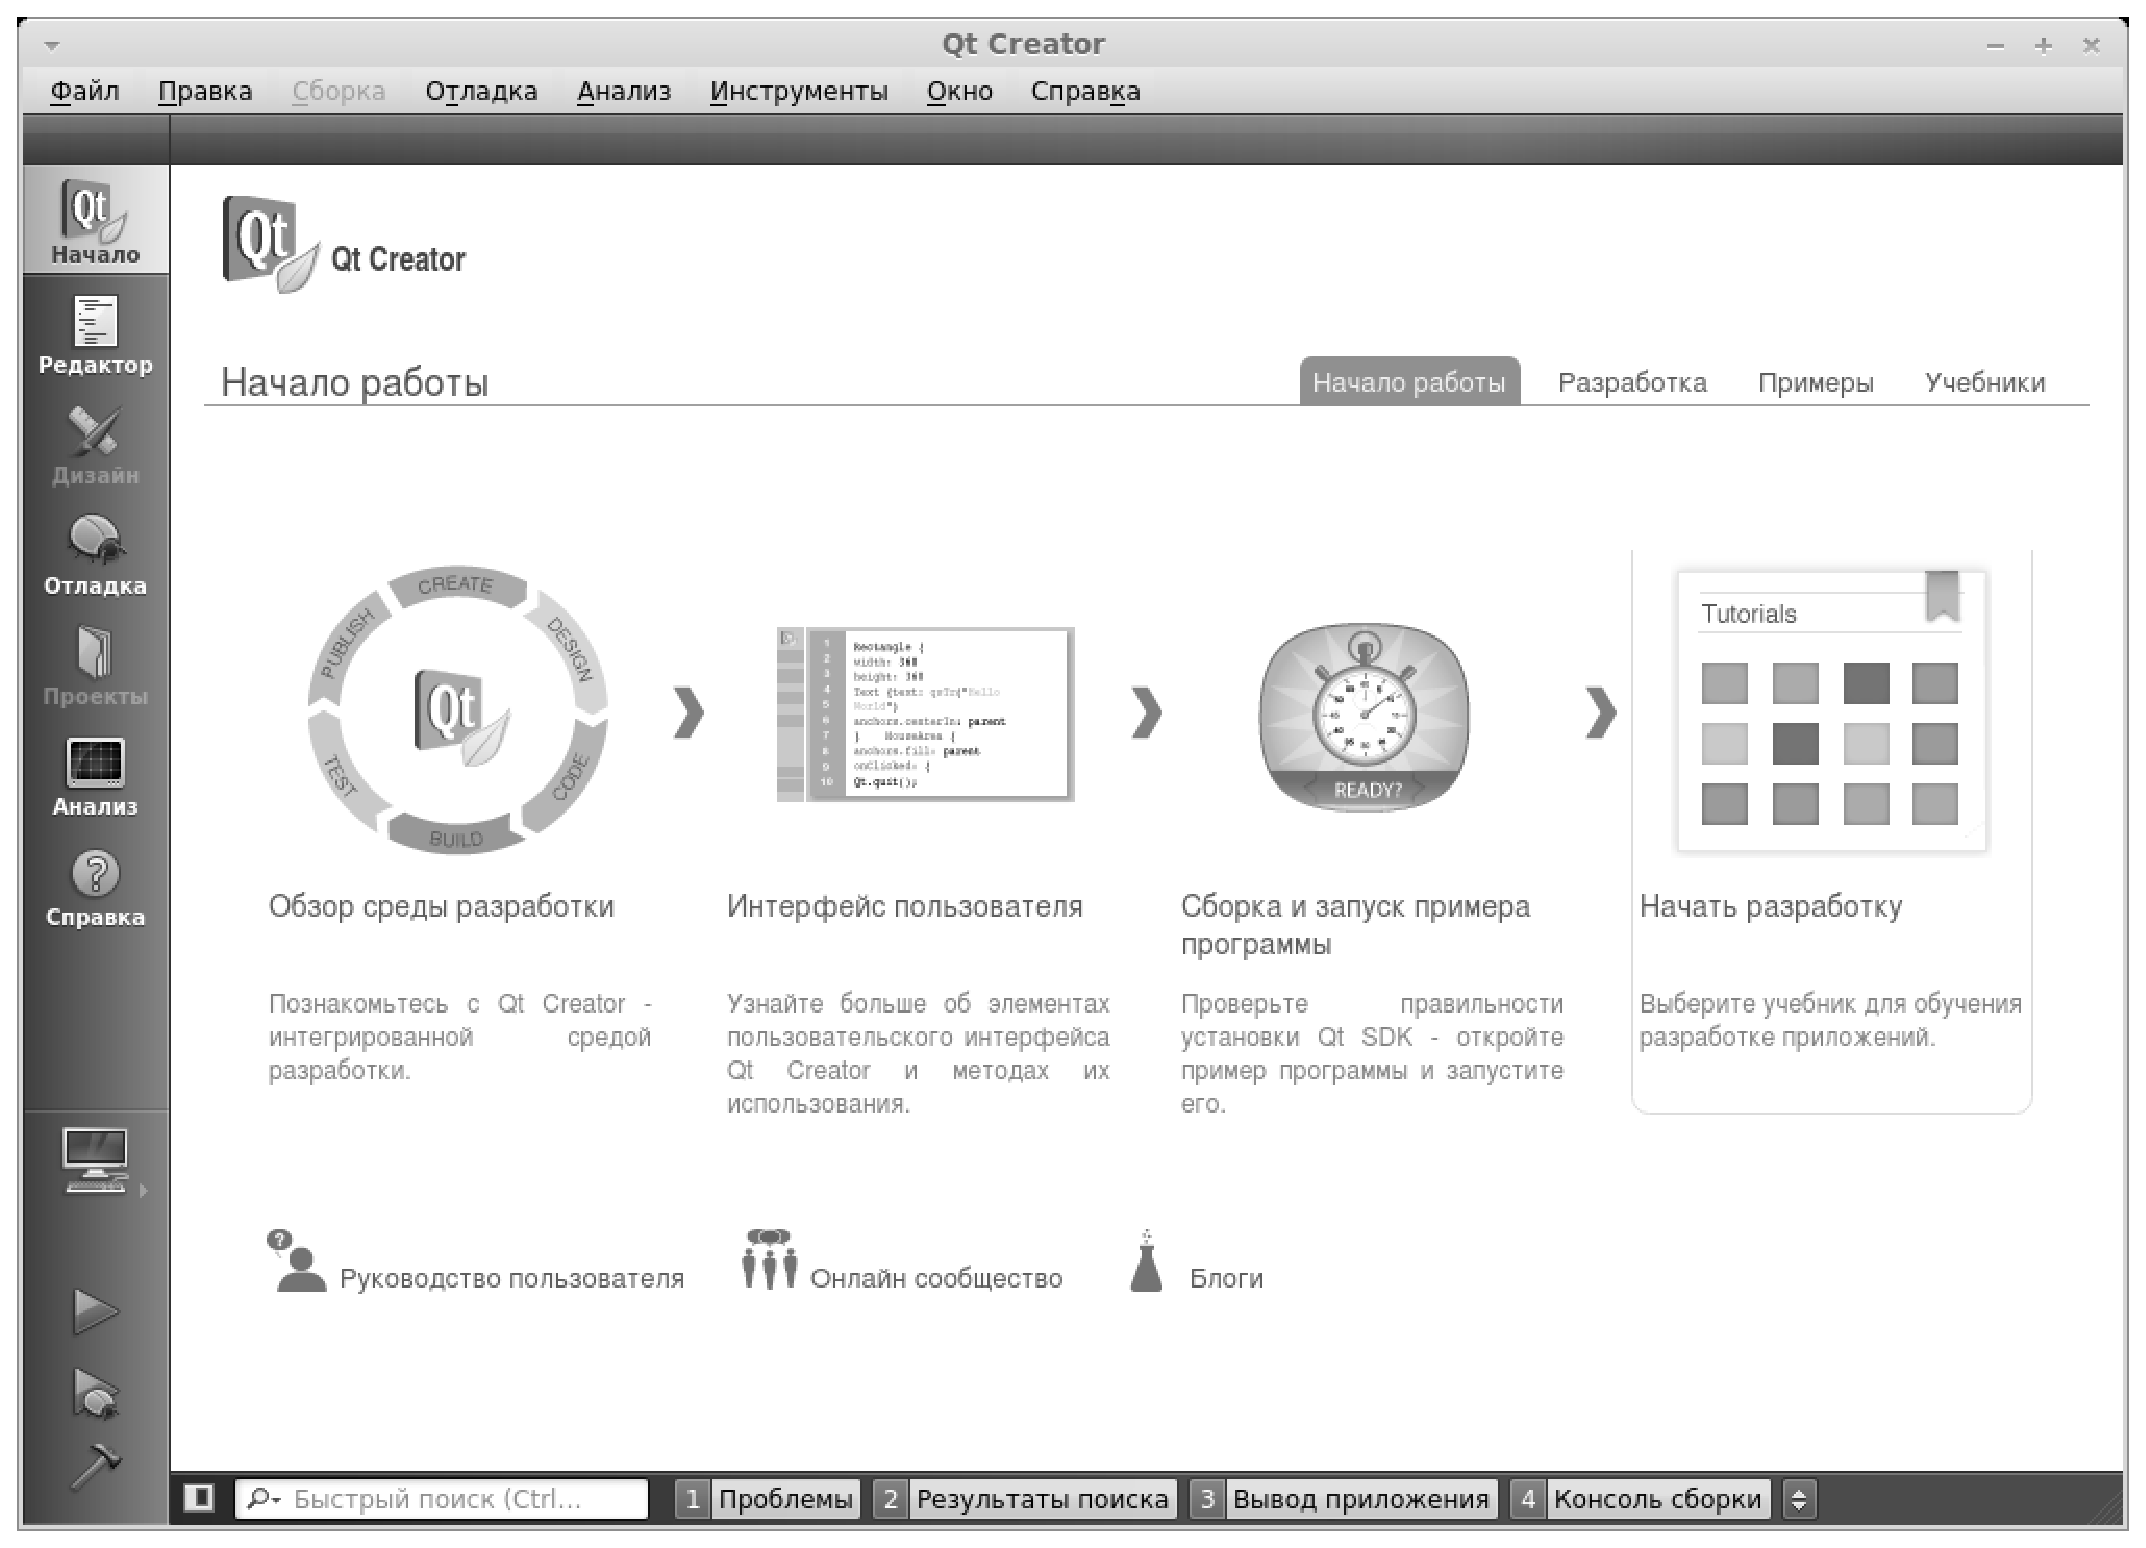
\includegraphics[width=0.7\textwidth]{img/ris_1_1_rus}
\caption{Окно \Sys{Qt Creator}}
\label{ch01:refDrawing0}
\end{center}
\end{figure}
При работе в \Sys{Qt Creator} вы находитесь в одном из режимов:

\begin{enumerate}
\item \Emph{Welcome} (Начало) --- отображает экран приветствия, позволяя быстро загружать недавние сессии или отдельные
проекты. Этот режим можно увидеть при запуске \Sys{Qt Creator} без указания ключей командной строки.
\item \Emph{Edi}t (Редактор) --- позволяет редактировать файлы проекта и исходных кодов. Боковая панель слева
предоставляет различные виды для перемещения между файлами.
\item \Emph{Debug} (Отладка) --- предоставляет различные способы для просмотра состояния программы при отладке.
\item \Emph{Projects} (Проекты) --- используется для настройки сборки, запуска и редактирования кода.
\item \Emph{Analyze} (Анализ) --- в Qt интегрированы современные средства анализа кода разрабатываемого приложения.
\item \Emph{Help} (Справка) --- используется для вывода документации библиотеки Qt и \Sys{Qt Creator}.
\item \Emph{Output} (Вывод) --- используется для вывода подробных сведений о проекте.
\end{enumerate}

Рассмотрим простейшие приёмы работы в среде \Sys{Qt Creator} на примере \index{Консольное приложение!создание}создания
консольного приложения для решения задачи \ref{ch01:prg1}. Для этого можно поступить одним из способов:

\begin{enumerate}
\item В меню \Emph{File} (Файл) выбрать команду \Emph{New File or Project} (Новый файл или проект) (комбинация
клавиш \Emph{Ctrl+N}).
\item Находясь в режиме \Emph{Welcome} (Начало) главного окна QtCreator (рис. \ref{ch01:refDrawing0}) щёлкаем по ссылке
\Emph{Develop} (Разработка) и выбираем команду Create Project (Создать проект).
\end{enumerate}

После это откроется окно, подобное представленному на рис.~\ref{ch01:refDrawing1}. Для создания простейшего консольного
приложения выбираем \Emph{Non-Qt Project} (Проект без использования \Sys{Qt}) --- \Emph{Plain \Sys{C++} Project} (Простой проект
на языке~\Sys{С++}).

Далее выбираем имя проекта и каталог для его размещения (см. рис.~\ref{ch01:refDrawing2})\footnote{Рекомендуем для
каждого проекта выбирать отдельный каталог. Проект --- это несколько
взаимосвязанных между собой файлов и каталогов.}. Следующие два этапа создания нашего первого приложения оставляем без
изменения\footnote{О назначении этих этапов будет рассказано в дальнейших разделах книги.}. После чего окно \Sys{IDE Qt
Creator} будет подобно представленному на рис.~\ref{ch01:refDrawing3}. Заменим текст «Hello, Word» стандартного
приложения, на текст программы решения задачи~\ref{ch01:prg1}.

\begin{figure}[htb]
\begin{center}
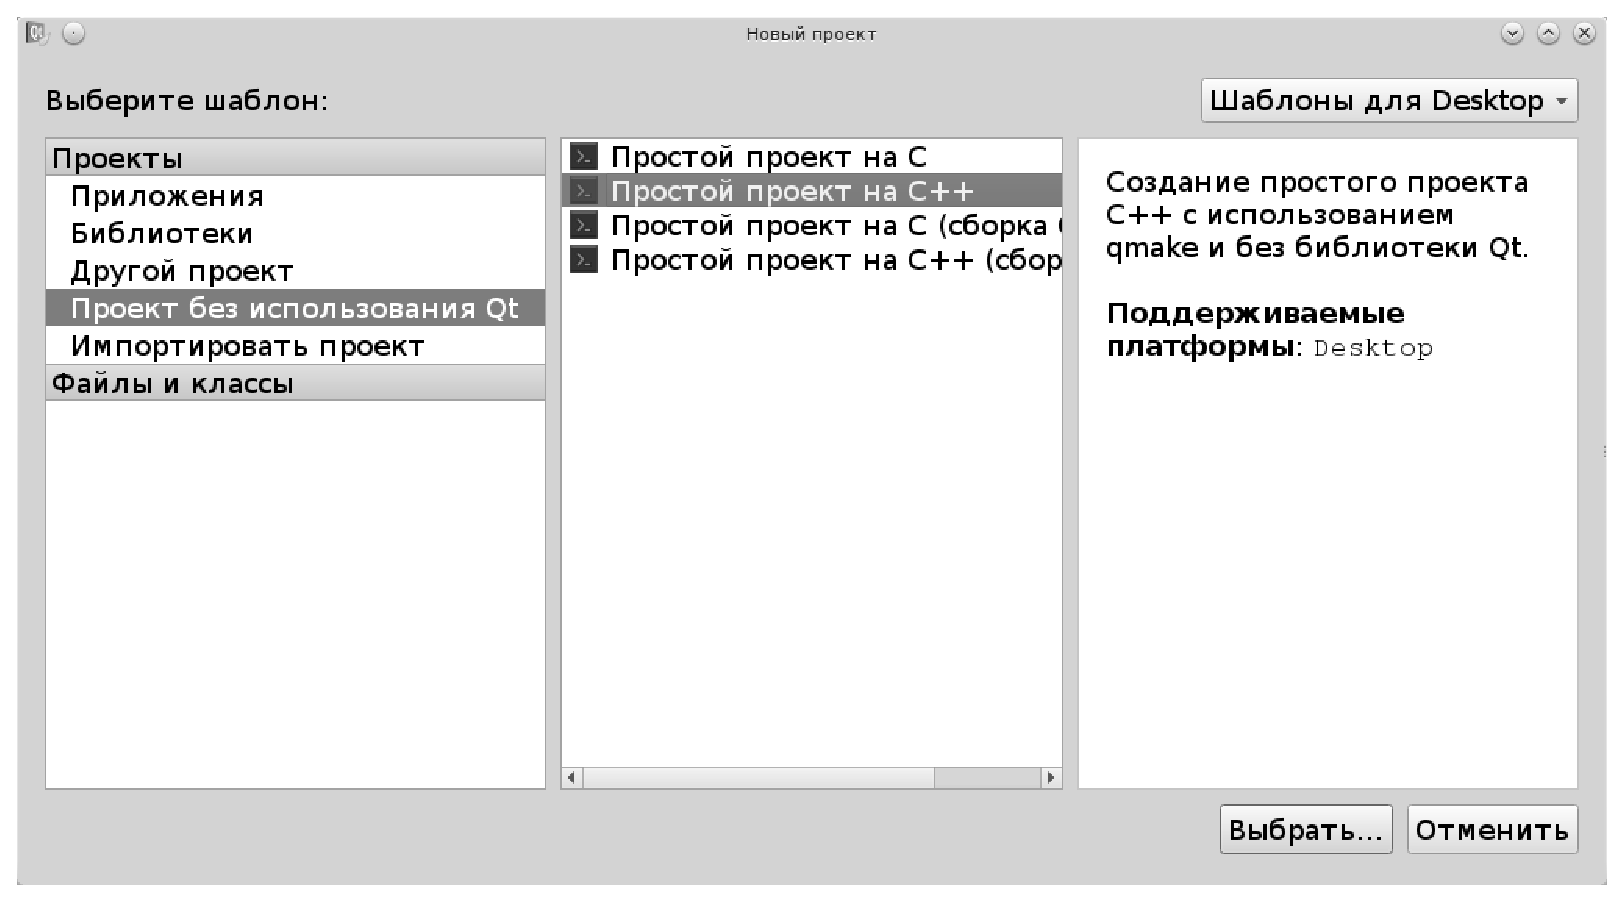
\includegraphics[width=0.7\textwidth]{img/ris_1_2_rus}
\caption{Окно выбора типа приложения в \Sys{Qt Creator}}
\label{ch01:refDrawing1}
\end{center}
\end{figure}

\begin{figure}[htb]
\begin{center}
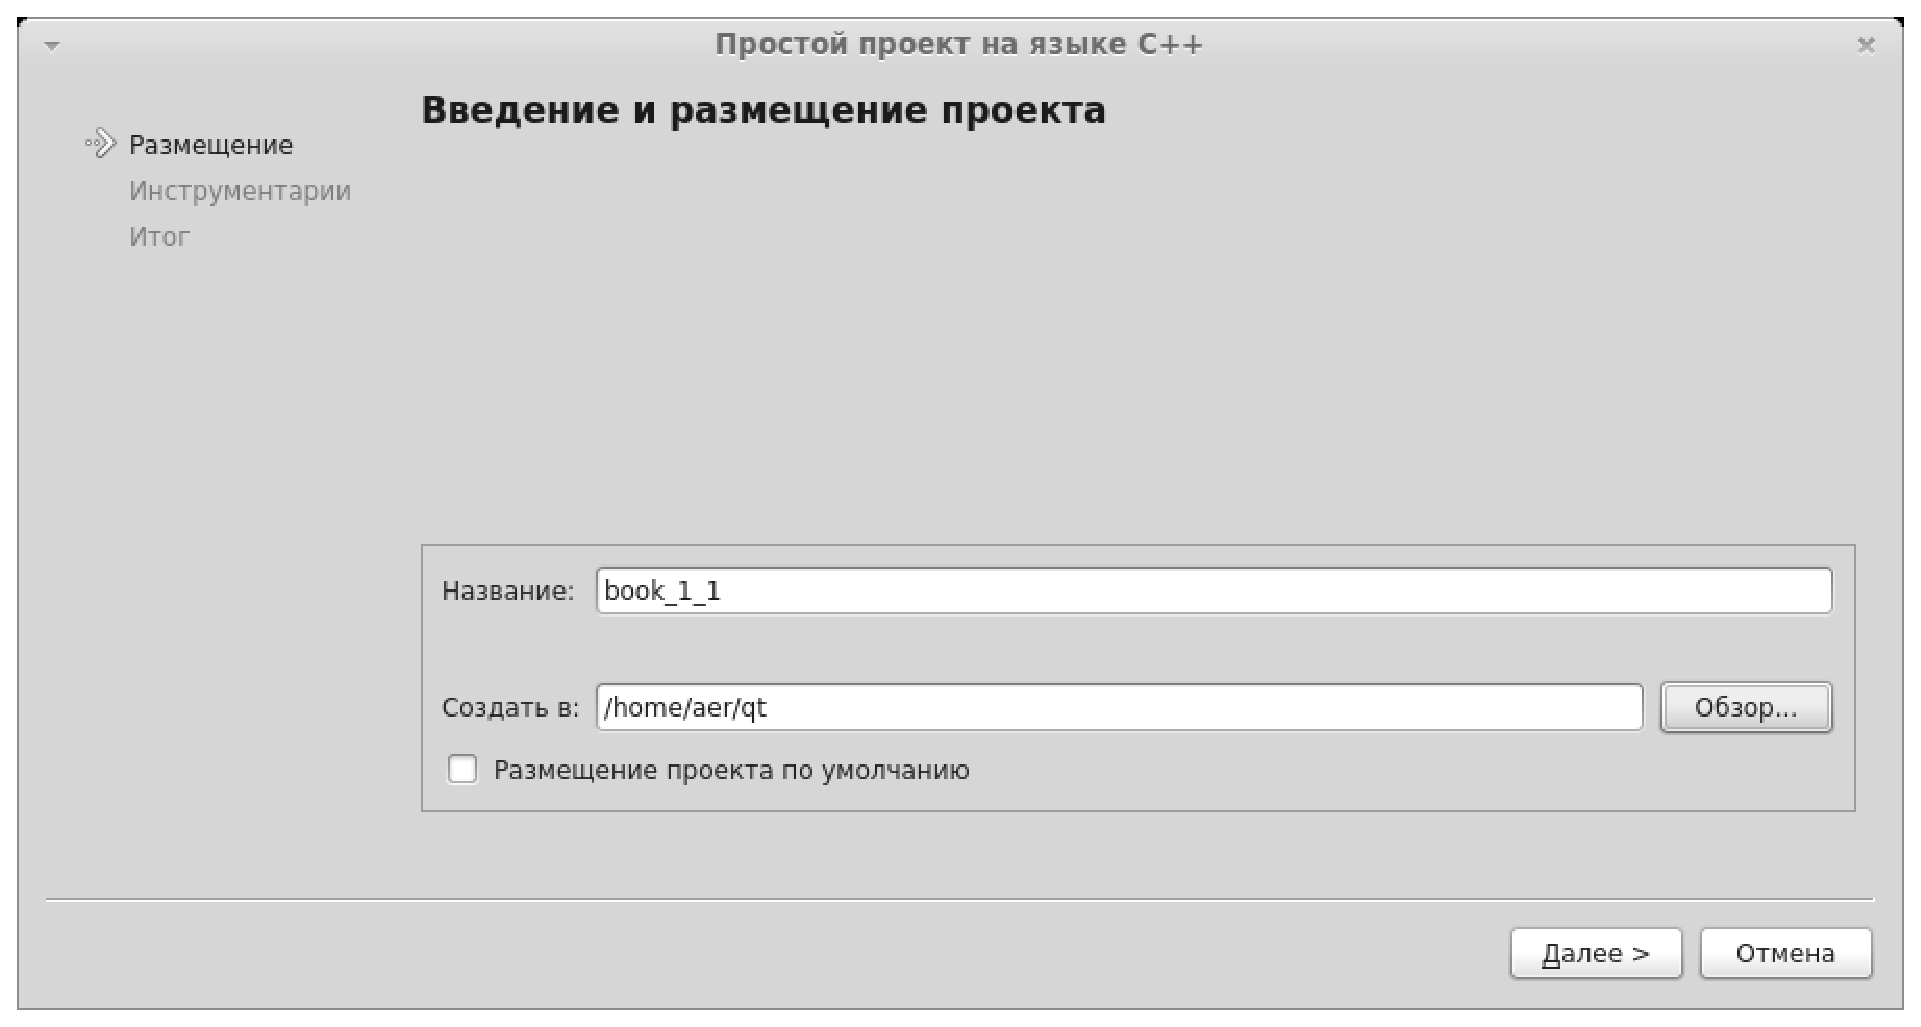
\includegraphics[width=0.7\textwidth]{img/ris_1_3_rus}
\caption{Выбор имени и каталога нового проекта}
\label{ch01:refDrawing2}
\end{center}
\end{figure}

Для сохранения текста программы можно воспользоваться командой \Emph{Сохранить} или \Emph{Сохранить всё} из меню
\Emph{Файл}. Откомпилировать и \index{Консольное приложение!запуск}запустить программу можно одним из следующих
способов:

\begin{figure}[htb]
\begin{center}
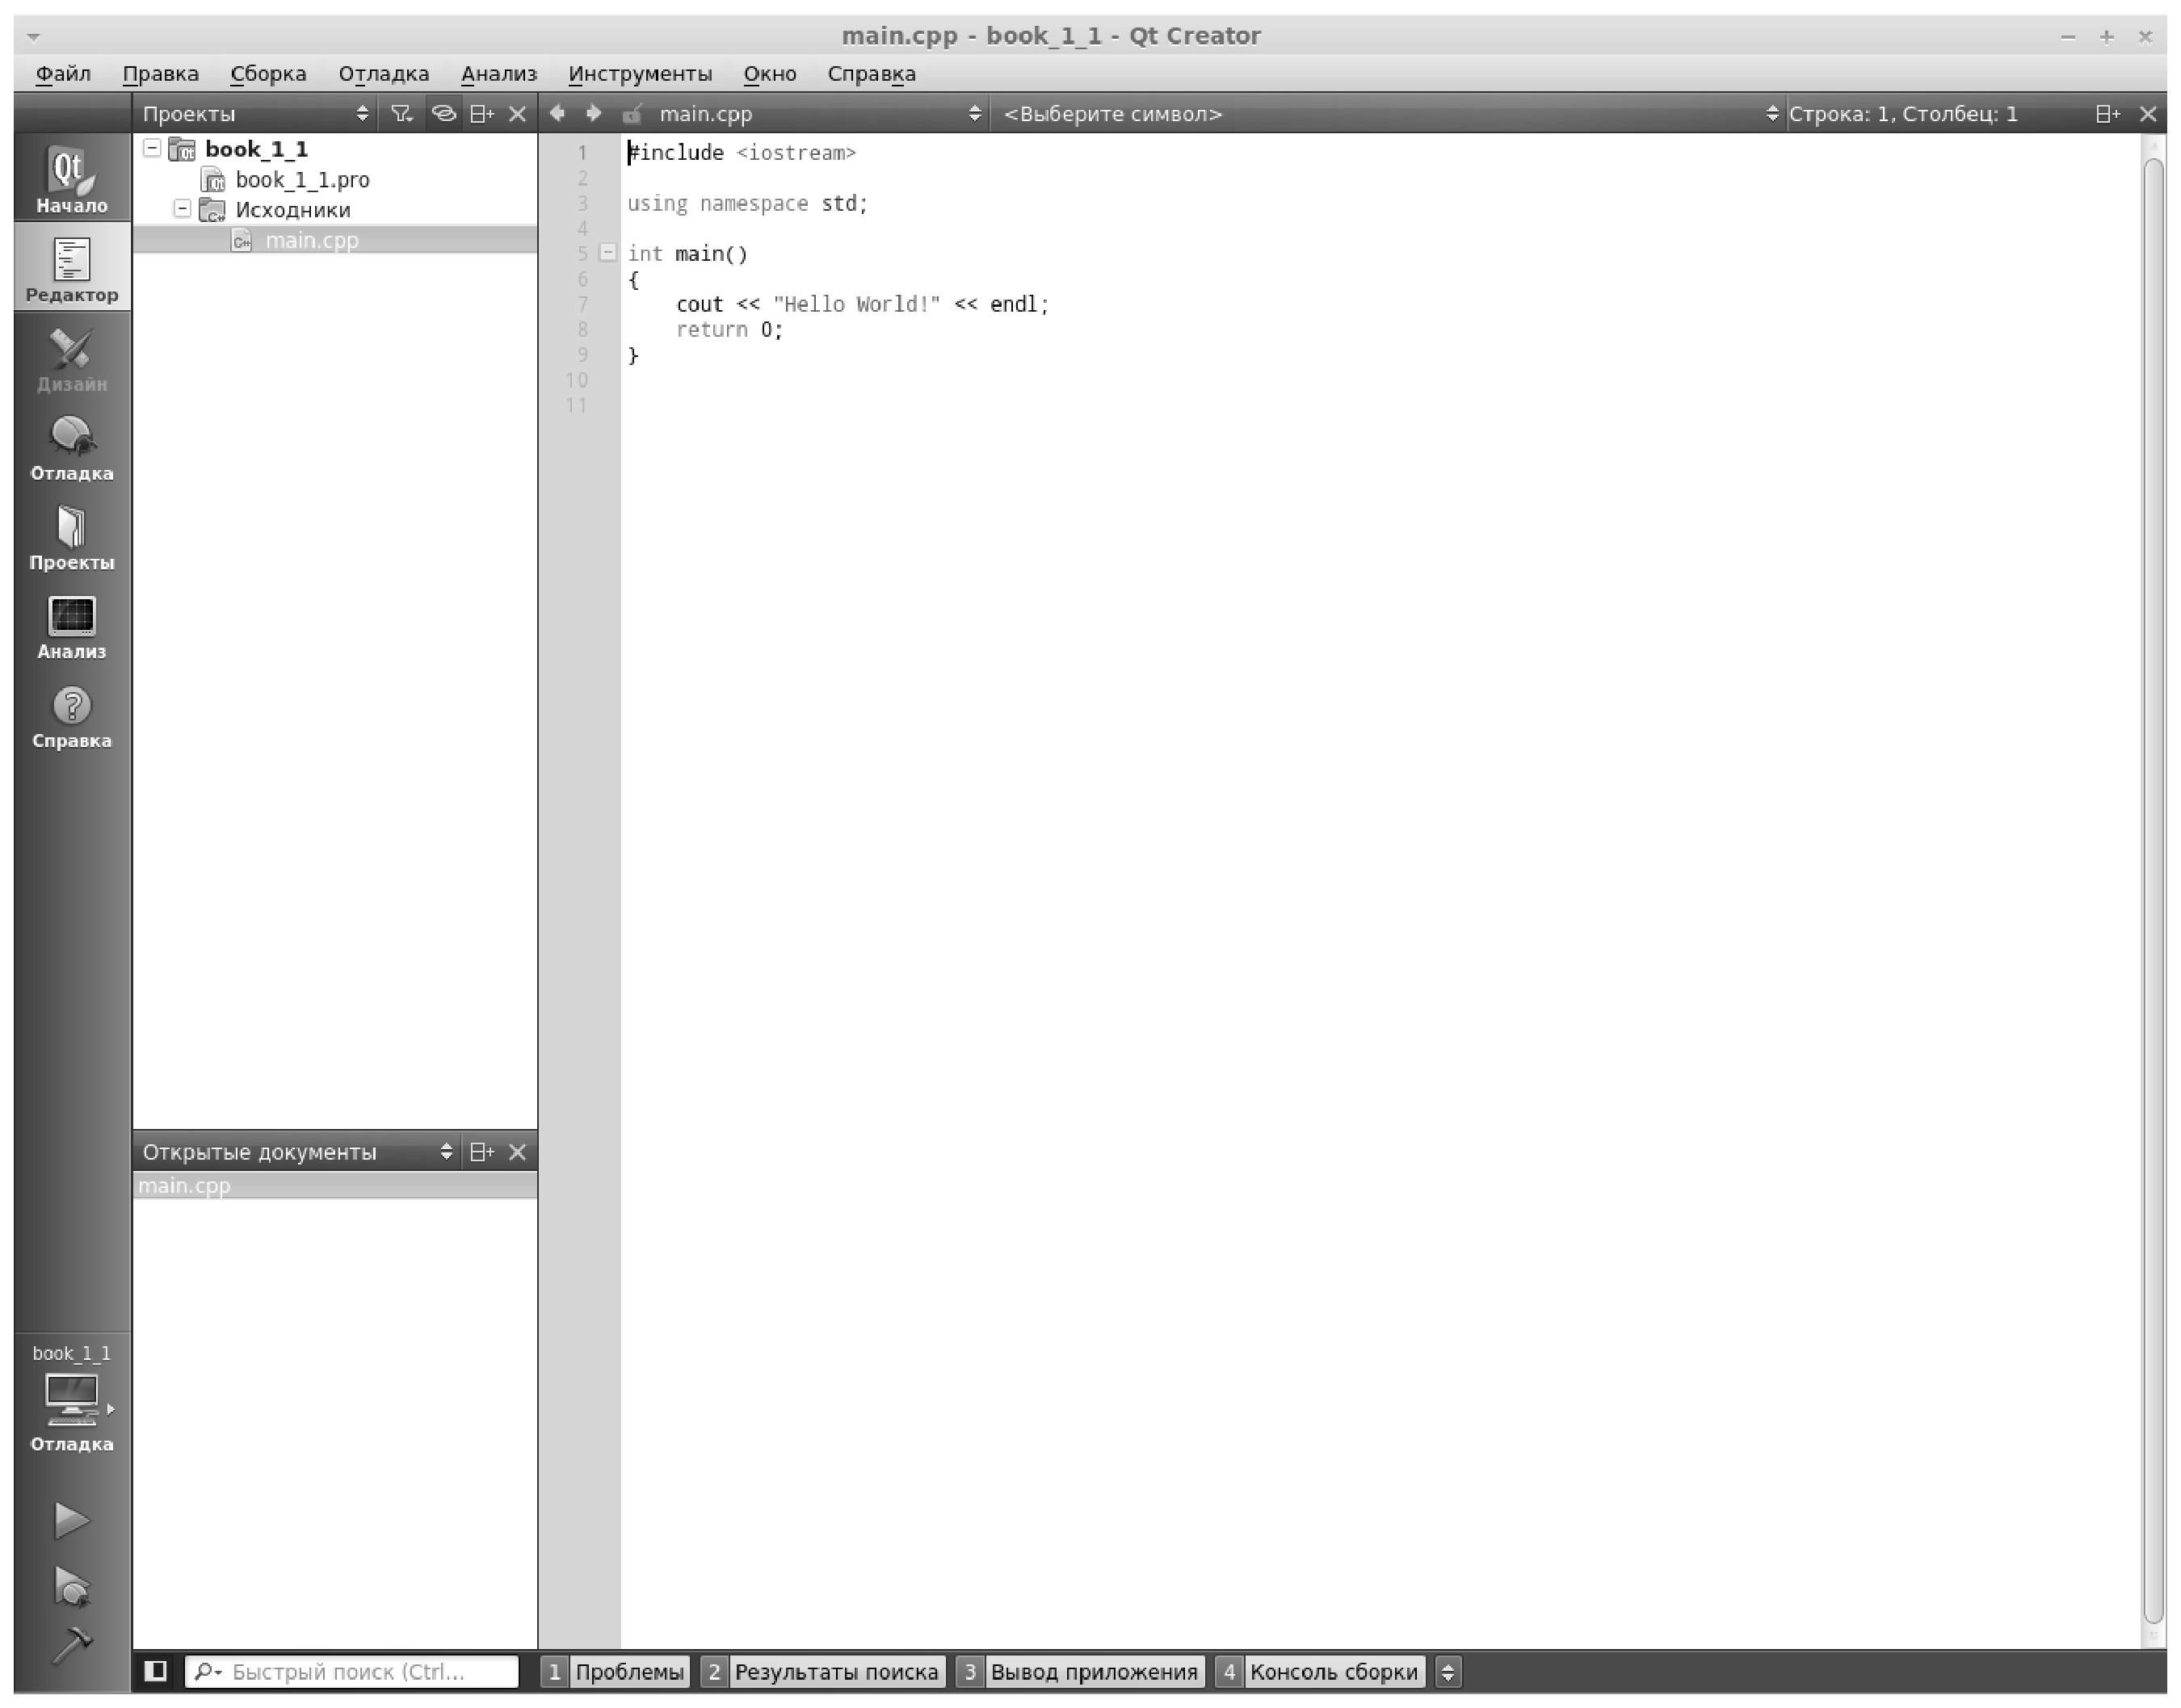
\includegraphics[width=0.7\textwidth]{img/ris_1_4_rus}
\caption{Главное окно создания консольного приложения}
\label{ch01:refDrawing3}
\end{center}
\end{figure}

\begin{enumerate}
\item Пункт меню \Emph{Сборка-Запустить}.
\item Нажать на клавиатуре комбинацию клавиш Ctrk+R.
\item Щёлкнуть по кнопке Запустить (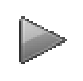
\includegraphics[scale=0.33]{img/rightarrow}).
\end{enumerate}
Окно с результатами работы программы представлено на рис. \ref{ch01:refDrawing4}.
\begin{figure}[htb]
\begin{center}
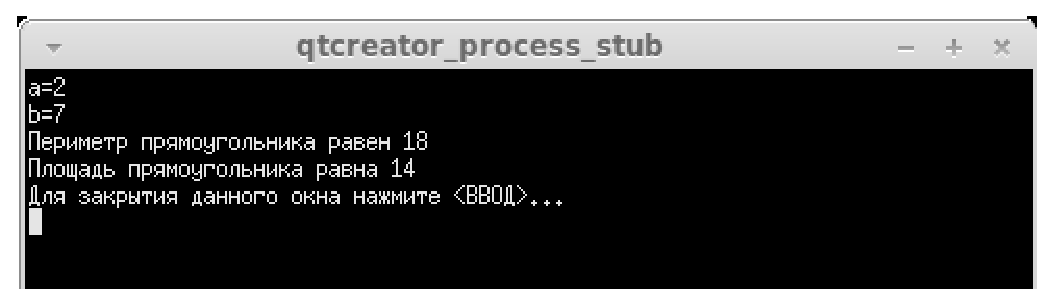
\includegraphics[width=0.7\textwidth]{img/ris_1_5}
\caption{Результаты работы программы решения задачи~\ref{ch01:prg1}}
\label{ch01:refDrawing4}
\end{center}
\end{figure}

Авторы сталкивались с тем, что в некоторых дистрибутивах Ubuntu Linux и Linux Mint после установки \Sys{Qt Creator} не
запускались консольные приложения. Если читатель столкнулся с подобной проблемой, скорее всего надо корректно настроить
терминал, который отвечает за запуск приложений в консоли. Для этого вызываем команду Tools --- Options --- Environment
(см. рис.~\ref{ch01:refDrawing5}). Параметр \Emph{Terminal} (Терминал) должен быть таким же, как показано на рис.
\ref{ch01:refDrawing5}. Проверьте установлен ли в Вашей системе пакет xterm, и при необходимости доставьте его. После
этого не должно быть проблем с запуском консольных приложений.

\begin{figure}[htb]
\begin{center}
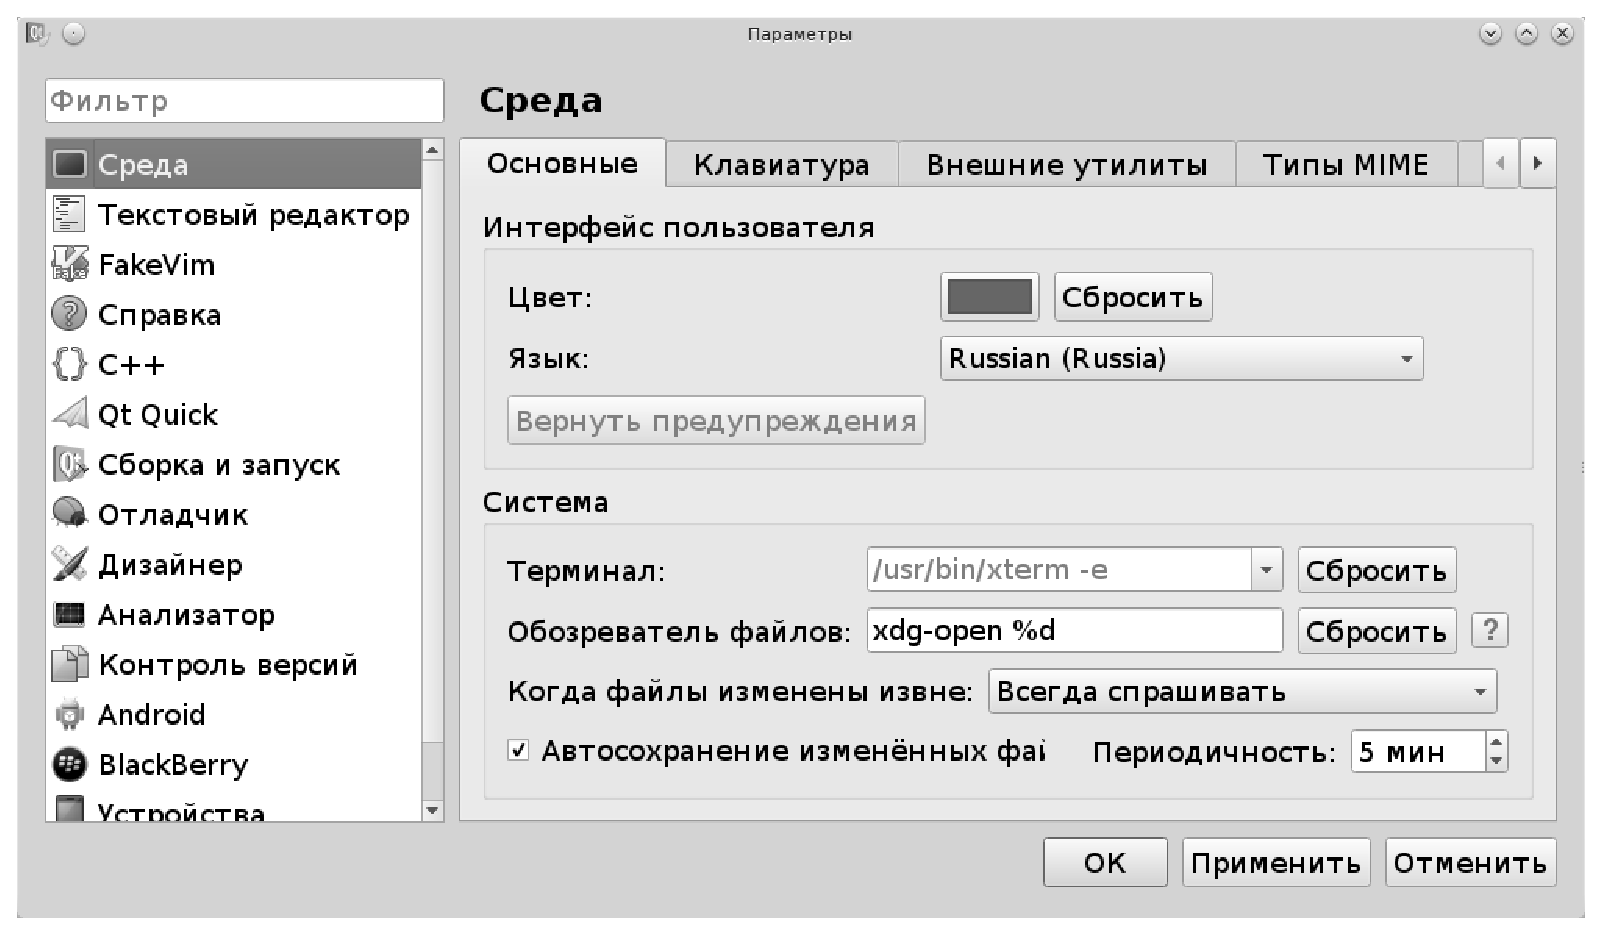
\includegraphics[width=0.7\textwidth]{img/ris_1_6}
\caption{Окно настроек среды \Sys{Qt Creator}}
\label{ch01:refDrawing5}
\end{center}
\end{figure}


Аналогичным образом можно создавать и запускать любое консольное приложение.

Дальнейшее знакомство со средой \Sys{Qt Creator} продолжим, решая следующую задачу.

\prg{Заданы длины трёх сторон треугольника $a$, $b$ и $c$ (см. рис.~\ref{ch01:refDrawing6}). 
Вычислить площадь и периметр треугольника.}{ch01:prg2}

\begin{figure}[htb]
\begin{center}
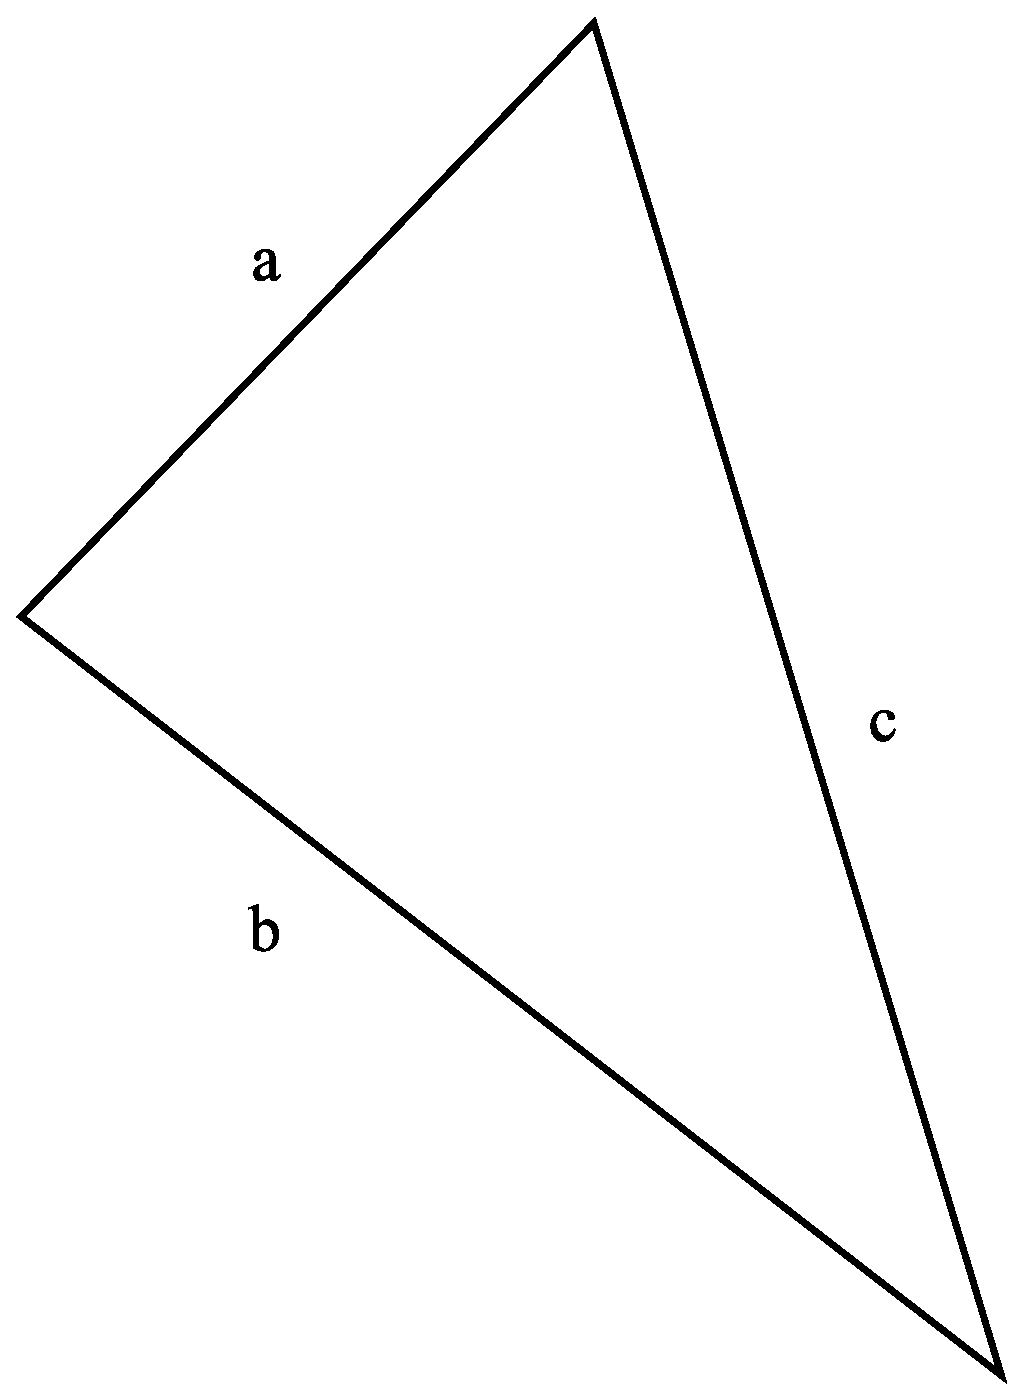
\includegraphics[width=0.3\textwidth]{img/ris_1_7}
\caption{Треугольник}
\label{ch01:refDrawing6}
\end{center}
\end{figure}

Для решения задачи можно воспользоваться формулой Герона 

$S=\sqrt{\frac{p}{2}\left(\frac{p}{2}-a\right)\left(\frac{p}{2}-b\right)\left(\frac{p}{2}-c\right)}$, 
где $p=a+b+c$ --- периметр.

Решение задачи можно разбить на следующие этапы:

\begin{enumerate}
\item  Определение значений $a$, $b$ и $c$ (ввод величин $a$, $b$, $c$ с клавиатуры в память компьютера).
\item  Расчёт значений $p$ и $s$ по приведённым выше формулам.
\item Вывод $p$ и $s$ на экран дисплея.
\end{enumerate}
Ниже приведён текст программы. Сразу заметим, что в тексте могут встречаться строки, начинающие с двух наклонных (//).
Это комментарии. \emph{Комментарии} не являются обязательными элементами программы и ничего не сообщают компьютеру, 
они поясняют человеку, читающему текст программы, назначение отдельных элементов программы. В книге комментарии 
будут широко использоваться для пояснения
отдельных участков программы.
\begin{lstlisting}
#include <iostream> 
#include <math.h> 
using namespace std; 
int main() 
{ 
    float a,b,c,s,p; 
    cout<<"`Введите длины сторон треугольника`"<<endl; 
//`Ввод значений длин треугольника` a,b,c.
    cin>>a>>b>>c; 
//`Вычисление периметра треугольника`.
    p=a+b+c; 
//`Вычисление площади треугольника`.
    s=sqrt(p/2*(p/2-a)*(p/2-b)*(p/2-c));
//`Вывод на экран дисплея значений площади и периметра треугольника.` 
    cout<<"`Периметр треугольника равен` "<<p<<", `его площадь равна` "<<s<<endl; 
    return 0; 
}
\end{lstlisting}

Кроме используемой в предыдущей программе библиотеки \Sys{iostream}, в строке 2 подключим библиотеку
\index{Библиотека!math.h}\Sys{math.h}, которая служит для использования математических 
функций языка \Sys{С}(\Sys{С++}). В данной
программе используется функция извлечения квадратного корня --- \index{Функция!sqrt(x)}\emph{sqrt(x)}. Остальные
операторы (ввода, вывода, вычисления значений переменных) аналогичны используемым в предыдущей программе.

Таким образом, выше были рассмотрены самые простые программы (линейной структуры), которые предназначены для ввода
исходных данных, расчёта по формулам и вывода результатов.


\chapter[Общие сведения о языке \Sys{С++}]{Общие сведения о языке \Sys{С++}}\label{gl02}
В этой главе читатель познакомится с основными элементами языка \Sys{С++}: алфавитом, переменными, константами, типами данных,
основными операциями, стандартными функциями, структурой программы и средствами ввода вывода данных.

\section[Алфавит языка]{Алфавит языка}
Программа на языке \Sys{С++} может содержать следующие символы:
\begin{itemize}
\item прописные, строчные латинские буквы A, B, C, …, x, y, z и знак подчеркивания;
\item арабские цифры от 0 до 9;
\item специальные знаки: “ \{ \} , {\textbar} [ ] ( ) + --- / \% * . {\textbackslash} ‘ : ? {<} = {>} !
\& \# \~{} ; \^{}
\item символы пробела, табуляции и перехода на новую строку.
\end{itemize}

Из символов алфавита формируют ключевые слова и идентификаторы. \index{Ключевые слова}{Ключевые слова}
 --- это зарезервированные слова, которые имеют специальное значение для компилятора и используются только в том смысле, в
котором они определены (операторы языка, типы данных и т.п.). \index{Идентификатор}Идентификатор ---
это имя программного объекта, представляющее собой совокупность букв, цифр и символа подчеркивания. Первый символ
идентификатора --- буква или знак подчеркивания, но не цифра. Идентификатор не может содержать пробел. Прописные и
строчные буквы в именах различаются, например, \Sys{ABC}, \Sys{abc}, \Sys{Abc} --- 
три различных имени. Каждое имя (идентификатор) должно быть уникальным в пределах функции и не совпадать с ключевыми
словами. 

В тексте программы можно использовать \index{Комментарии}комментарии. Если текст начинается с двух
символов «косая черта» // и заканчивается символом перехода на новую строку или заключен между
символами /* и */, то компилятор его игнорирует. 

\begin{lstlisting}
/* `\Sys{Комментарий может}`
 `\Sys{выглядеть так!}`*/
//`А если вы используете такой способ,`
//`то каждая строка должна начинаться`
//`с двух символов «косая черта».`
\end{lstlisting}

Комментарии удобно использовать как для пояснений к программе, так и для временного исключения фрагментов программы при
отладке.

\section[Данные]{Данные}
Для решения задачи в любой программе выполняется обработка каких-либо данных. Данные хранятся в памяти компьютера и
могут быть самых различных типов: целыми и вещественными числами, символами, строками, массивами. \index{Типы
данных}{Типы данных} определяют способ хранения чисел или символов в памяти компьютера. Они задают
размер ячейки, в которую будет записано то или иное значение, определяя тем самым его максимальную величину или
точность задания. Участок памяти (ячейка), в котором хранится значение определенного типа, называется
\index{Переменная}переменной. У переменной есть \index{Переменная!имя}имя
(идентификатор) и \index{Переменная!значение}значение. Имя служит для обращения к области памяти, в
которой хранится значение. Во время выполнения программы значение переменной можно изменить. Перед использованием любая
переменная должна быть описана. \index{Переменная!описание}Оператор описания переменных в языке \Sys{С++}
имеет вид:
\begin{itemize}
\item[] \Sys{тип имя\_переменной;}
\end{itemize}
или
\begin{itemize}
\item[] \Sys{тип список\_переменных;}
\end{itemize}

Типы данных языка \Sys{С++} можно разделить на основные и составные.

К \index{Типы данных!основные}основным типам данных языка относят:
\begin{itemize}
\item \Sys{char} --- символьный; 
\item \Sys{int} --- целый; 
\item \Sys{float} --- с плавающей точкой; 
\item \Sys{double} --- двойной точности; 
\item \Sys{bool} --- логический.
\end{itemize}

Для формирования других типов данных используют основные типы и так называемые спецификаторы. Типы данных, созданные на
базе стандартных типов с использованием спецификаторов, называют \index{Типы данных!составные}составными типами данных. 
В \Sys{С++} определены четыре спецификатора типов данных:
\begin{itemize}
\item \Sys{short} --- короткий;
\item \Sys{long} --- длинный;
\item \Sys{signed} --- знаковый;
\item \Sys{unsigned} --- беззнаковый.
\end{itemize}

Далее будут рассмотрены назначение и описание каждого типа.

\subsection[Символьный тип]{Символьный тип}
Данные типа \Sys{char} в памяти компьютера всегда занимают один байт\footnote{В кодировке utf каждый символ
кириллицы занимает 2 байта.}. Это связано с тем, что обычно под величину символьного типа отводят столько памяти,
сколько необходимо для хранения любого из 256 символов клавиатуры. \index{Типы данных!символьный}Символьный тип может
быть со знаком или без знака (табл. \ref{ch02:refTable0}).

\noindent
\begin{longtable}{|l|r|r|}
\caption{Символьные типы данных} \label{ch02:refTable0}\\
\hline
\Emph{Тип}&\Emph{Диапазон}&\Emph{Размер}\\ 
\hline \hline 
\endfirsthead
\multicolumn{3}{c}%
{{\tablename\ \thetable{} --- продолжение}} \\
\hline
\Emph{Тип}&\Emph{Диапазон}&\Emph{Размер}\\ 
\hline \hline
\endhead
\Sys{char} & –128…127 & 1 байт\\\hline
\Sys{unsigned char} & 0…255 &1 байт\\\hline
\Sys{signed char} &–128…127 &1 байт\\\hline
\end{longtable}

Пример описания символьных переменных:
\begin{lstlisting}
char c, str; //`\Sys{Описаны две символьные переменные.}`
\end{lstlisting}
При работе с символьными данными нужно помнить, что если в выражении встречается одиночный символ, он должен быть
заключен в одинарные кавычки. Например, \Sys{'a'}, \Sys{'b'}, \Sys{'+'},
\Sys{'3'}.

Последовательность символов, то есть строка, при использовании в выражениях заключается в двойные кавычки:
\Sys{”Hello!”}.

\subsection[Целочисленный тип]{Целочисленный тип}
Переменная типа \Sys{int} в памяти компьютера может занимать либо два, либо четыре байта. Это зависит от
разрядности процессора. 

Диапазоны значений \index{Типы данных!целый}целого типа представлены в таблице \ref{ch02:refTable1}. По умолчанию все
целые типы считаются знаковыми, т.е. спецификатор \Sys{signed} можно не указывать.


\noindent
\begin{longtable}{|l|c|l|}
\caption{Целые типы данных} \label{ch02:refTable1}\\
\hline
\Emph{Тип}&\Emph{Диапазон}&\Emph{Размер}\\
\hline \hline
\endfirsthead
\multicolumn{3}{c}%
{{\tablename\ \thetable{} --- продолжение}} \\
\hline
\Emph{Тип}&\Emph{Диапазон}&\Emph{Размер}\\
\hline \hline
\endhead
\Sys{int} &–2147483647 …  2147483647 &4 байта\\\hline
\Sys{unsigned int} &0 … 4294967295 &4 байта\\\hline
\Sys{signed int} &–2147483647 …  2147483647 &4 байта\\\hline
\Sys{short int} &–32767 … 32767 &2 байта\\\hline
\Sys{long int} &–2147483647 … 2147483647 &4 байта\\\hline
\Sys{unsigned short int} &0 … 65535 &2 байта\\\hline
\Sys{signed short int} &–32767 … 32767 &2 байта\\\hline
\Sys{long long int} &–($2^{63}$–1) … ($2^{63}$–1) &8 байт\\\hline
\Sys{signed long int} & –2147483647 … 2147483647 &4 байта\\\hline
\Sys{unsigned long int} &0 … 4294967295 &4 байта\\\hline
\Sys{unsigned long long int} &0 … ${2^{64}}$–1  &8 байт\\\hline
\end{longtable}

Пример описания целочисленных данных:
\begin{lstlisting}
int a, b, c;
unsigned long int A, B, C;
\end{lstlisting}

\subsection[Вещественный тип]{Вещественный тип}
Внутреннее представление \index{Типы данных!вещественный}вещественного числа в памяти компьютера отличается от
представления целого числа. Число с плавающей точкой представлено в  экспоненциальной форме
$mE\pm p$, где $m$ --- мантисса (целое или дробное число с
десятичной точкой), $p$ --- порядок (целое число). Для того чтобы перевести число в экспоненциальной
форме к обычному представлению с фиксированной точкой, необходимо мантиссу умножить на десять в степени порядок.
Например, 

 $-6.42E+2=-6.42\cdot 10^{2}=-642$,

$3.2E-6=3.2\cdot 10^{-6}=0.0000032$

Обычно величины типа \Sys{float} занимают 4 байта, из которых один двоичный разряд отводится под знак, 8
разрядов под порядок и 23 под мантиссу. Поскольку старшая цифра мантиссы всегда равна 1, она не хранится.

Величины типа \Sys{double} занимают 8 байт, в них под порядок и мантиссу отводится 11 и 52 разряда
соответственно. Длина мантиссы определяет точность числа, а дли-на порядка его диапазон. Спецификатор типа
\Sys{long} перед именем типа \Sys{double} указывает, что под величину отводится 10 байт.

Диапазоны значений вещественного типа представлены в таблице~\ref{ch02:refTable2}.


\noindent
\begin{longtable}{|l|c|l|}
\caption{Вещественные типы данных} \label{ch02:refTable2}\\
\hline
\Emph{Тип}&\Emph{Диапазон}&\Emph{Размер}\\
\hline \hline
\endfirsthead
\multicolumn{3}{c}%
{{\tablename\ \thetable{} --- продолжение}} \\
\hline
\Emph{Тип}&\Emph{Диапазон}&\Emph{Размер}\\
\hline \hline
\endhead
\Sys{float} &3.4Е-38 … 3.4E+38 &4 байта\\\hline
\Sys{double} &1.7Е-308 … 1.7E+308 &8 байт\\\hline
\Sys{long double} &3.4Е-4932 … 3.4E+4932 &10 байт\\\hline
\end{longtable}

Пример описания вещественных переменных:
\begin{lstlisting}
double x1,x2,x3;
float X, Y, Z;
\end{lstlisting}

\subsection[Логический тип]{Логический тип}
Переменная \index{Типы данных!логический}типа \Sys{bool} может принимать только два значения
\Sys{true} (истина) или \Sys{false} (ложь). Любое значение не равное нулю интерпретируется
как \Sys{true}, а при преобразовании к целому типу принимает значение равное 1. Значение
\Sys{false} представлено в памяти как 0.

Пример описания данных логического типа:
\begin{lstlisting}
bool F, T;
\end{lstlisting}

\subsection[Тип void]{Тип void}
Множество значений этого типа пусто. Он используется для определения функций, которые не возвращают значения, для
указания пустого списка аргументов функции, как базовый тип для указателей и в операции приведения типов.

\section[Константы]{Константы}
\index{Константа}Константы это величины, которые не изменяют своего значения в процессе выполнения
программы. \index{Константа!описание}Оператор описания константы имеет вид:

\Sys{сonst тип имя\_константы = значение;}

Константы в языке \Sys{С++} могут быть целыми, вещественными, символьными или строковыми. Обычно компилятор определяет тип
константы по внешнему виду, но существует возможность и явного указания типа, например,

\Sys{const double pi=3.141592653589793}

Кроме того, константа может быть определена с помощью директивы\footnote{Структура программы и директивы описаны в
п.~\ref{ch02:8}}
\Sys{\#define}. Эта директива служит для замены часто использующихся констант, ключевых слов,
операторов или выражений некоторыми идентификаторами. Идентификаторы, заменяющие текстовые или числовые константы,
называют {именованными константами}. Основная форма синтаксиса директивы следующая:
\begin{lstlisting}
#define `\Sys{идентификатор текст}`
\end{lstlisting}
Например, 
\begin{lstlisting}
#define PI 3.141592653589793
int main()
...
\end{lstlisting}

\section[Структурированные типы данных]{\Sys{Структурированные типы данных}}
\index{Типы данных!структурированные}Структурированный тип данных характеризуется множественностью
образующих его элементов. В C++ это массивы, строки, структуры и файлы.

\index{Массив}Массив --- совокупность данных одного и того же типа\footnote{Подробно работа с
одномерными и двумерными массивами описана в главах \ref{ch05} и \ref{ch06}.}. Число элементов массива 
фиксируется при описании типа и в
процессе выполнения программы не изменяется.

В общем виде массив можно описать так:

\Sys{тип имя [размерность\_1][размерность\_2]\dots [размерность\_N];}

Например,
\begin{lstlisting}
float x[10]; //`Описан массив из 10 целых чисел.`
int a[3][4]; //`Описан двумерный массив, матрица из 3-х строк и 4-х столбцов.`
double b[2][3][2];//`Описан трехмерный массив.`
\end{lstlisting}
Для доступа к элементу массива достаточно указать его порядковый номер, а если
массив многомерный (например, таблица), то несколько номеров:

\Sys{имя\_массива[номер\_1][номер\_2]\dots [номер\_N]}


Например: \Sys{x[5]}, \Sys{a[2][3]}, \Sys{b[1][2][2]}.

Элементы массива в \Sys{С++} нумеруются с нуля. Первый элемент, всегда имеет 
номер ноль, а номер последнего элемента на
единицу меньше заданной при его описании размерности: 
\begin{lstlisting}
char C[5]; //`Описан массив из 5 символов, нумерация от 0 до 4.`
\end{lstlisting}

\index{Строка}Строка --- последовательность символов\footnote{Работа со строками описана в главе~\ref{ch08}}. В
\Sys{С++} строки описывают как массив элементов типа \Sys{char}. Например:
\begin{lstlisting}
char s[25];//`Описана строка из 25 символов.`
\end{lstlisting}
\index{Структура}{Структура}\footnote{Работа со структурами описана в главе~\ref{ch09}.} это тип данных,
который позволяет объединить разнородные данные и обрабатывать их как единое целое.

Например
\begin{lstlisting}
struct fraction //`Объявлена структура правильная дробь.`
{
//`Определяем поля структуры:`
int num; //`поле числитель,`
int den; //`поле знаменатель.`
}
...
fraction d, D[20]; //`Определена переменная d, массив D[20], типа fraction.`
...
d.num; //`Обращение к полю num переменной d.`
D[4].den; //`Обращение к полю den четвертого элемента массива D.`
\end{lstlisting}

\section[Указатели]{\Sys{Указатели}}
Указатели широко применяются в \Sys{С++}. Можно сказать, что именно наличие указателей сделало этот язык
удобным для системного программирования. С другой стороны это одна из наиболее сложных для освоения возможностей \Sys{С++}.
Идея работы с указателями состоит в том, что пользователь работает с адресом ячейки памяти.

Как правило, при обработке оператора объявления переменной 

\Sys{тип имя\_переменной;}

компилятор автоматически выделяет память под переменную
\Sys{имя\_переменной} в соответствии с указанным типом:
\begin{lstlisting}
char C; //`Выделена память под символьную переменную C`
\end{lstlisting}
Доступ к объявленной переменной осуществляется по ее имени. При
этом все обращения к переменной заменяются на адрес ячейки памяти, в которой хранится ее значение. При завершении
программы или функции, в которой была описана переменная, память автоматически освобождается.

Доступ к значению переменной можно получить иным способом --- определить собственные
переменные для хранения адресов памяти. Такие переменные называют
\index{Указатель}указателями. С помощью указателей можно обрабатывать массивы,
строки и структуры, создавать новые переменные в процессе выполнения программы, передавать адреса фактических
параметров функциям и адреса функций в качестве параметров.

Итак, указатель это переменная, значением которой является
адрес памяти, по которому хранится объект определенного типа (другая переменная). Например, если
С это переменная типа
char, а Р --- указатель на
С, значит в Р находится адрес по которому в
памяти компьютера хранится значение переменной С.

Как и любая переменная, указатель должен быть объявлен. При
объявлении указателей всегда указывается тип объекта, который будет храниться по данному адресу:

\Sys{тип *имя\_переменной;}

Например:
\begin{lstlisting}
int *p; //`По адресу, записанному в переменной p, будет храниться переменная типа int`
\end{lstlisting}
Звездочка в описании указателя, относится непосредственно к имени, поэтому чтобы объявить несколько
указателей, ее ставят перед именем каждого из них: 
\begin{lstlisting}
float *x, y, *z; //`Описаны указатели на вещественные числа x и z, сами вещественные значения *x, *z, а так же вещественная переменная y, её адрес --- \&y.`
\end{lstlisting}
\section[Операции и выражения]{Операции и выражения}\label{ch02:6}
\index{Выражение}Выражение задает порядок выполнения действий над данными и состоит из
\index{Операнд}операндов (констант, переменных, обращений к функциям), круглых скобок и знаков
операций. \index{Операции}Операции делятся на \index{Операции!унарные}унарные
(например, \Sys{-с}) и \index{Операции!бинарные}бинарные
(например,  \Sys{а+b}). В таблице \ref{ch02:refTable3} представлены основные операции языка \Sys{С++}.


\noindent
\begin{longtable}{|l|l|}
\caption{Основные операции языка \Sys{С++}} \label{ch02:refTable3}\\
\hline
\Emph{Операция}&\Emph{Описание}\\
\hline \hline
\endfirsthead
\multicolumn{2}{c}%
{{\tablename\ \thetable{} --- продолжение}} \\
\hline
\Emph{Операция}&\Emph{Описание}\\
\hline \hline
\endhead
\multicolumn{2}{|c|}{\Emph{Унарные операции}}\\\hline
\Sys{++} & увеличение значения на единицу\\\hline
\Sys{{}-{}-} & уменьшение значения на единицу\\\hline
\Sys{\~} & поразрядное отрицание\\\hline
\Sys{!} & логическое отрицание\\\hline
\Sys{-} & арифметическое отрицание (унарный минус)\\\hline
\Sys{+} & унарный плюс\\\hline
\Sys{\&} & взятие адреса\\\hline
\Sys{*} & разадресация\\\hline
\Sys{(type)} & преобразование типа\\\hline
\multicolumn{2}{|c|}{\Emph{Бинарные операции}}\\\hline
\Sys{+} & сложение\\\hline
\Sys{-} & вычитание\\\hline
\Sys{*} & умножение\\\hline
\Sys{/} & деление\\\hline
\Sys{\%} & остаток от деления\\\hline
\Sys{{<}{<}} & сдвиг влево\\\hline
\Sys{{>}{>}} & сдвиг вправо\\\hline
\Sys{{<}} & меньше\\\hline
\Sys{{>}} & больше\\\hline
\Sys{{<}=} & меньше или равно\\\hline
\Sys{{>}=} & больше или равно\\\hline
\Sys{==} & равно\\\hline
\Sys{!=} & не равно\\\hline
\Sys{\&} & поразрядная конъюнкция (И)\\\hline
\Sys{\^} & поразрядное исключающее ИЛИ\\\hline
\Sys{{\textbar}} & поразрядная дизъюнкция (ИЛИ)\\\hline
\Sys{\&\&} & логическое И\\\hline
\Sys{{\textbar}{\textbar}} & логическое ИЛИ\\\hline
\Sys{=} & присваивание\\\hline
\Sys{*=} & умножение с присваиванием\\\hline
\Sys{/=} & деление с присваиванием\\\hline
\Sys{+=} & сложение с присваиванием\\\hline
\Sys{-=} & вычитание с присваиванием\\\hline
\Sys{\%=} & остаток от деления с присваиванием\\\hline
\Sys{{<}{<}=} & сдвиг влево с присваиванием\\\hline
\Sys{{>}{>}=} & сдвиг вправо с присваиванием\\\hline
\Sys{\&=} & поразрядная конъюнкция с присваиванием\\\hline
\Sys{{\textbar}=} &поразрядная дизъюнкция с присваиванием\\\hline
\Sys{\^=} &поразрядное исключающее ИЛИ с присваиванием\\\hline
\multicolumn{2}{|c|}{\Emph{Другие операции}}\\\hline
\Sys{?} & условная операция\\\hline
\Sys{,} & последовательное вычисление\\\hline
\Sys{sizeof} & определение размера\\\hline
\Sys{(тип)} & преобразование типа\\\hline
\end{longtable}

Перейдем к подробному рассмотрению основных операций языка.

\subsection[Операции присваивания]{Операции присваивания}
Обычная \index{Операции!присваивания}операция присваивания имеет вид:

\Sys{имя\_переменной=значение;}


где \Sys{значение} это выражение, переменная, константа или функция. Выполняется операция так. Сначала
вычисляется значение выражения указанного в правой части оператора, а затем его результат записывается в область
памяти, имя которой указано слева.

Например,
\begin{lstlisting}
b=3;     //`Переменной b присваивается значение равное трем.`
a=b;     //`Переменной а присваивается значение b.`
c=a+2*b; //`Переменной c присваивается значение выражения.`
c=c+1;   //`Значение переменой с увеличивается на единицу.`
a=a*3;   //`Значение переменой а увеличивается в три раза.`
\end{lstlisting}

\prg{Пусть в переменной \Sys{а} хранится значение равное 3, а в
переменную \Sys{b} записали число 5. Поменять местами значения переменных \Sys{а} и
\Sys{b}.}{ch02:prg1}

Для решения задачи понадобится дополнительная переменная \Sys{c} (см. рис.~\ref{ch02:refDrawing0}). 
В ней временно сохраняется значение переменной \Sys{а}. Затем, значение переменной
\Sys{b} записывается в переменную \Sys{a}, а значение переменной \Sys{c} в
переменную \Sys{b}.
\begin{lstlisting}
c=a; //`Шаг 1. с=3`
a=b; //`Шаг 2. a=5`
b=c; //`Шаг 3. b=3`
\end{lstlisting}

\begin{figure}[htb]
\begin{center}
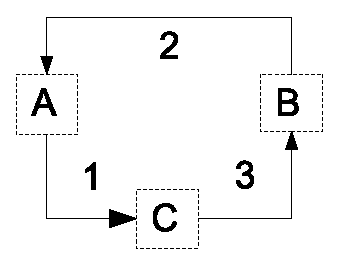
\includegraphics[width=0.3\textwidth]{img/ris_2_1}
\caption{Использование буферной переменной}
\label{ch02:refDrawing0}
\end{center}
\end{figure}

Если в операторе присваивания левая и правая часть это переменные разных типов, то \emph{происходит
преобразование}: значение переменной в правой части преобразуется к типу переменной в левой части. Следует учитывать,
что при этом можно потерять информацию или получить другое значение.

В \Sys{С++} существует возможность присваивания нескольким переменным одного и того же значения. Такая операция называется
\index{Операции!множественного присваивания}\emph{множественным присваиванием} и в общем виде может быть
записана так:

\Sys{имя\_1 = имя\_2 = … = имя\_N = значение;}

Запись \Sys{a=b=c=3.14159/6;}
означает, что переменным \Sys{a}, \Sys{b} и \Sys{c} было присвоено одно и то же
значение \Sys{3.14159/6}.

Операции $+=$, $-=$, $*=$, $/=$ называют \index{Операции!составного присваивания}\emph{составным присваиванием}. В
таких операциях при вычислении выражения стоящего справа используется значение переменной из левой части, например так:
\begin{lstlisting}
x+=p; //`Увеличение x на p, то же что и x=x+p.`
x-=p; //`Уменьшения x на p, то же что и x=x-p.`
x*=p; //`Умножение x на p, то же что и x=x*p.`
x/=p; //`Деление x на p, то же что и x=x/p.`
\end{lstlisting}

\subsection[Арифметические операции]{Арифметические операции}
Операции $+$, $-$, $*$, $/$ относят к
\index{Операции!арифметические}\emph{арифметическим операциям}. Их назначение понятно и не требует
дополнительных пояснений. При программировании арифметических выражений следует придерживаться простых правил.
Соблюдать очерёдность выполнения арифметических операций. Сначала выполняются операции умножения и деления (1-й
уровень), а затем сложения и вычитания (2-й уровень). Операции одного уровня выполняются последовательно друг за
другом. Для изменения очерёдности выполнения операций используют скобки. Таблица \ref{ch02:refTable4} содержит примеры
записи алгебраических выражений.

\noindent
\begin{longtable}{|l|p{0.5\textwidth}|}
\caption{Примеры записи алгебраических выражений} \label{ch02:refTable4}\\
\hline
\Emph{Математическая запись}&\Emph{Запись на языке \Sys{С++}}\\
\hline \hline
\endfirsthead
\multicolumn{2}{c}%
{{\tablename\ \thetable{} --- продолжение}} \\
\hline
\Emph{Математическая запись}&\Emph{Запись на языке \Sys{С++}}\\
\hline \hline
\endhead
$\displaystyle 2\cdot a+b\cdot (c+d)$  & \Sys{2*a+b*(c+d)}\\\hline
$\displaystyle 3\cdot {\frac{a+b}{c+d}}$ & \Sys{3*(a+b)/(c+d)}\\\hline
$\displaystyle\frac{3\cdot a-2\cdot b}{c\cdot d}$ & \Sys{(3*a-2*b)/(c*d) или} \Sys{(3*a-2*b)/c/d}\\\hline
$\displaystyle\frac{(b-a)^2}{\displaystyle c+\displaystyle\frac{1}{d-2}}-\displaystyle\frac{a^2+1}{b^2+cd}$ & \Sys{(b-a)*(b-a)/(c+1/(d-2))-} \Sys{(a*a+1)/(b*b+c*d)}\\\hline
\end{longtable}

Операции \index{Операции!инкремента}\emph{инкремента} \Sys{++} и
\index{Операции!декремента}\emph{декремента} -{}-  так же причисляют к
арифметическим, так как они выполняют увеличение и уменьшение на единицу значения переменной. Эти операции имеют две
формы записи: префиксную (операция записывается перед операндом) и постфиксную (операция записывается после операнда).
Так, например оператор  \Sys{p=p+1;} можно представить в префиксной форме \Sys{++p;} и в
постфиксной \Sys{p++;}. Эти формы отличаются при использовании их в выражении. Если знак декремента
(инкремента) предшествует операнду, то сначала выполняется увеличение (уменьшение) значения операнда, а затем операнд
участвует в выражении. Например, 
\begin{lstlisting}
x=12;
y=++x; //`В переменных x и y будет храниться значение 13.`
\end{lstlisting}

Если знак декремента (инкремента) следует после операнда, то сначала операнд участвует в выражении, а затем выполняется
увеличение (уменьшение) значения операнда:
\begin{lstlisting}
x=12;
y=x++; //`Результат --- число 12 в переменной y, а в x --- 13.`
\end{lstlisting}

Остановимся на \index{Операции!целочисленной арифметики}\emph{операциях целочисленной
арифметики}. 

Операция целочисленного деления $/$ возвращает целую часть частного (дробная часть отбрасывается) в том
случае если она применяется к целочисленным операндам, в противном случае выполняется обычное деление: $11/4=2$ или
$11.0/4=2.75$.

Операция остаток от деления $\%$ применяется только к целочисленным операндам: $11\%4 = 3$.

К \index{Операции!битовой арифметики}\emph{операциям битовой арифметики} относятся
следующие операции: \Sys{\&}, \Sys{{\textbar}}, \Sys{\^{}},
\Sys{\~{}}, \Sys{{<}{<}}, \Sys{{>}{>}}. В
операциях битовой арифметики действия происходят над двоичным представлением целых чисел. 

\emph{Арифметическое И} (\Sys{\&}). Оба операнда переводятся в двоичную систему, затем над
ними происходит логическое поразрядное умножение операндов по следующим правилам: 

1\&1=1, 1\&0=0, 0\&1=0, 0\&0=0. 

Например, если \Sys{А=14} и \Sys{В=24}, то их двоичное представление ---
\Sys{А=0000000000001110} и \Sys{В=0000000000011000}. В результате логического умножения
\Sys{A and B} получим \Sys{0000000000001000} или 8 в десятичной системе
счисления (рис. \ref{ch02:refDrawing1}). Таким образом, \Sys{A\&B=14\&24=8}.

%\begin{figure}[htb]
%\begin{center}
%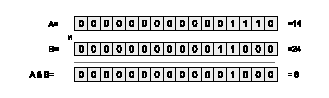
\includegraphics[width=0.5\textwidth]{img/ris_2_2}
%\caption{Пример логического умножения}
%\label{ch02:refDrawing1}
%\end{center}
%\end{figure}

%%%% рис 2 и 3 бок о бок
\begin{figure}[H]
\begin{floatrow}
\floatbox{figure}[.45\textwidth][\FBheight][t]
{\caption{Пример логического умножения}
\label{ch02:refDrawing1}}
{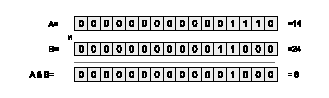
\includegraphics[width=0.45\textwidth,keepaspectratio]{img/ris_2_2}}\hspace*{0.05\textwidth}
%
\floatbox{figure}[.45\textwidth][\FBheight][b]
{\caption{Пример логического сложения}
\label{ch02:refDrawing2}}
{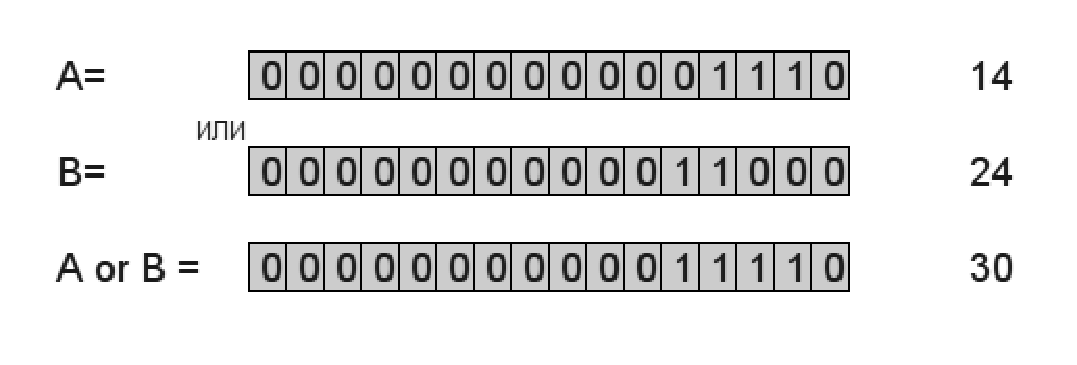
\includegraphics[width=0.45\textwidth,keepaspectratio]{img/ris_2_3}}
\end{floatrow}
\end{figure}


\emph{Арифметическое ИЛИ} ({\textbar}). Здесь также оба операнда переводятся в двоичную
систему, после чего над ними происходит логическое поразрядное сложение операндов по следующим правилам:

\Sys{1{\textbar}1=1, 1{\textbar}0=1, 0{\textbar}1=1, 0{\textbar}0=0.} 

Например, результат логического сложения чисел \Sys{А=14} и \Sys{В=24} будет равен \Sys{A or B=30} 
(рис.~\ref{ch02:refDrawing2}). 

%\begin{figure}[htb]
%\begin{center}
%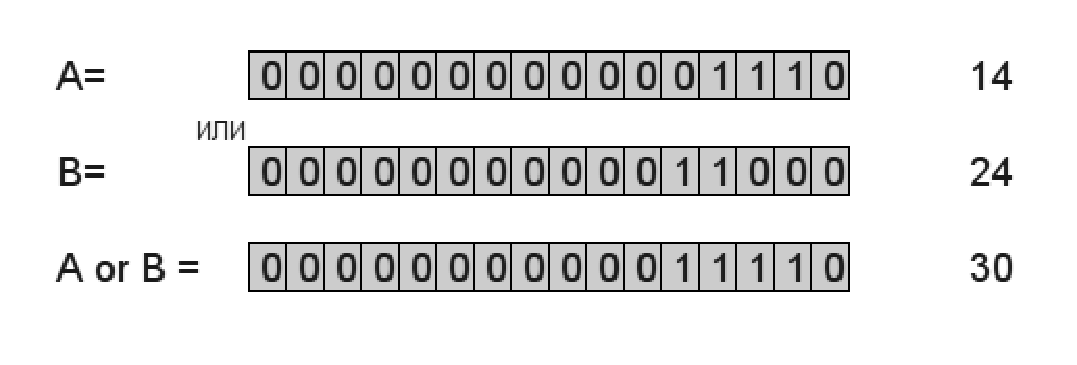
\includegraphics[width=0.5\textwidth]{img/ris_2_3}
%\caption{Пример логического сложения}
%\label{ch02:refDrawing2}
%\end{center}
%\end{figure}

\emph{Арифметическое исключающее ИЛИ} (\^{}). Оба операнда переводятся в двоичную
систему, после чего над ними происходит логическая поразрядная операция \^{} по следующим правилам:

\Sys{1\^{}1=0, 1\^{}0=1, 0\^{}1=1, 0\^{}0=0.}

\emph{Арифметическое отрицание} (\~{}). Эта операция выполняется над одним операндом.
Применение операции \~{} вызывает побитную инверсию двоичного представления числа 
(рис.~\ref{ch02:refDrawing3}).

\begin{figure}[htb]
\begin{center}
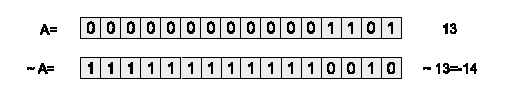
\includegraphics[width=0.5\textwidth]{img/ris_2_4}
\caption{Пример арифметического отрицания}
\label{ch02:refDrawing3}
\end{center}
\end{figure}

\emph{Сдвиг влево} (\Sys{M{<}{<}L}). Число
\Sys{M}, представленное в двоичной системе, сдвигается
влево на \Sys{L} позиций. Рассмотрим операцию \Sys{15 shl 3}. Число 15 в двоичной системе
имеет вид \Sys{1111}. При сдвиге его на 3 позиции влево получим \Sys{1111000}. В десятичной 
системе это двоичное число равно \Sys{120}.
Итак, \Sys{15 shl 3 =120} (рис.~\ref{ch02:refDrawing4}). Заметим, что сдвиг на один разряд влево соответствует
умножению на два, на два разряда --- умножению на четыре, на три --- умножению на восемь. Таким образом, операция
\Sys{M{<}{<}L} эквивалентна умножению числа \Sys{M} на 2 в степени \Sys{L}. 

%\begin{figure}[htb]
%\begin{center}
%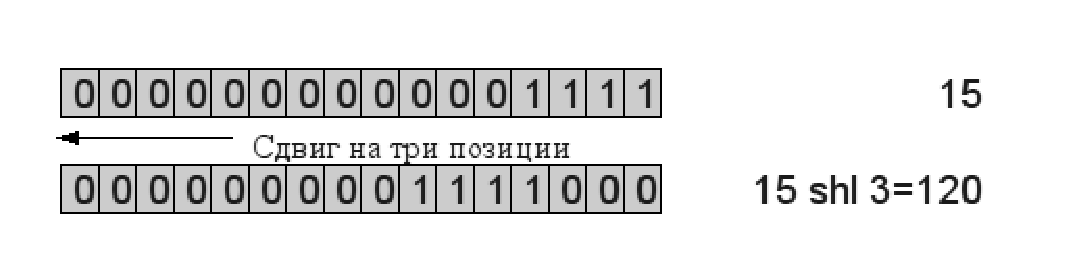
\includegraphics[width=0.5\textwidth]{img/ris_2_5}
%\caption{Пример операции «Сдвиг влево»}
%\label{ch02:refDrawing4}
%\end{center}
%\end{figure}

%%%% рис 5 и 6 бок о бок
\begin{figure}[H]
\begin{floatrow}
\floatbox{figure}[.45\textwidth][\FBheight][t]
{\caption{Пример операции <<Сдвиг влево>>}
\label{ch02:refDrawing4}}
{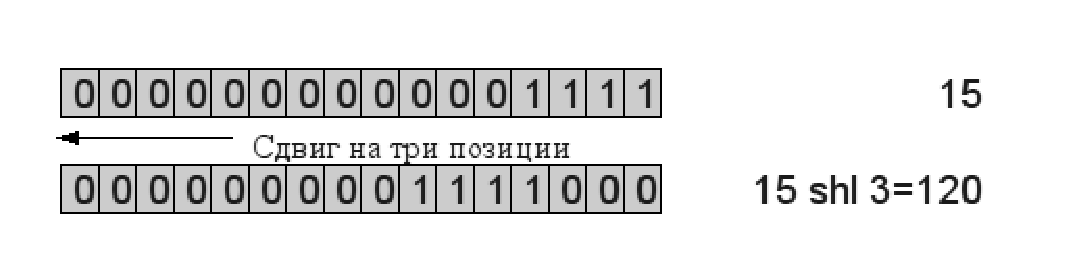
\includegraphics[width=0.45\textwidth,keepaspectratio]{img/ris_2_5}}\hspace*{0.05\textwidth}
%
\floatbox{figure}[.45\textwidth][\FBheight][b]
{\caption{Пример операции <<Сдвиг вправо>>}
\label{ch02:refDrawing5}}
{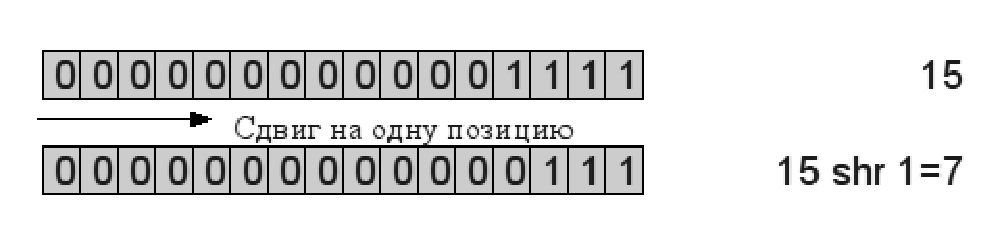
\includegraphics[width=0.45\textwidth,keepaspectratio]{img/ris_2_6}}
\end{floatrow}
\end{figure}


\emph{Сдвиг вправо} (\Sys{M{>}{>}L}). Число
\Sys{M}, представленное в двоичной системе, сдвигается вправо на 
\Sys{L} позиций, что эквивалентно целочисленному делению числа
\Sys{M} на 2 в степени \Sys{L}. Например, \Sys{15 shr 1=7} (рис.~\ref{ch02:refDrawing5}), \Sys{15 shr 3= 2}. 

%\begin{figure}[htb]
%\begin{center}
%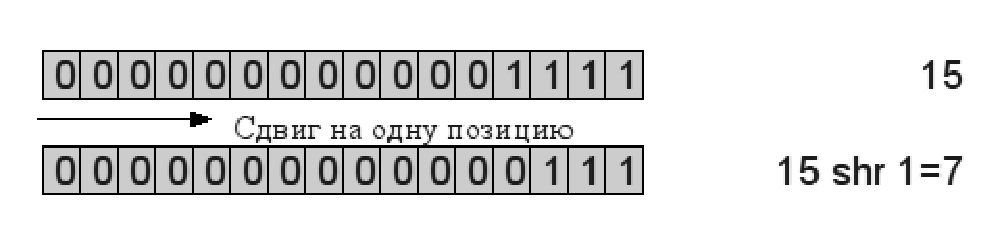
\includegraphics[width=0.5\textwidth]{img/ris_2_6}
%\caption{Пример операции «Сдвиг вправо»}
%\label{ch02:refDrawing5}
%\end{center}
%\end{figure}

\subsection[Логические операции]{Логические операции}
В \Sys{С++} определены следующие \index{Операции!логические}логические
операции {\textbar}{\textbar} (или), \Sys{\&\&} (и), \Sys{!} (не). Логические операции выполняются над логическими
значениями \Sys{true} (истина) и \Sys{false} (ложь). В языке \Sys{С++} ложь --- 0, истина --- любое
значение ${\neq}$ 0. В таблице~\ref{ch02:refTable5} приведены результаты логических операций.

\noindent
\begin{longtable}{|c|c|c|c|c|}
\caption{Логические операции} \label{ch02:refTable5}\\
\hline
\Emph{A}&\Emph{B}&\Emph{!A}&\Emph{A\&\&B}&\Emph{A{\textbar}{\textbar}B}\\
\hline \hline
\endfirsthead
\multicolumn{5}{c}%
{{\tablename\ \thetable{} --- продолжение}} \\
\hline
\Emph{A}&\Emph{B}&\Emph{!A}&\Emph{A\&\&B}&\Emph{A{\textbar}{\textbar}B}\\
\hline \hline
\endhead
0 & 0 & 1 & 0 & 0\\\hline
0 & 1 & 1 & 0 & 1\\\hline
1 & 0 & 0 & 0 & 1\\\hline
1 & 1 & 0 & 1 & 1\\\hline
\end{longtable}

\subsection[Операции отношения]{Операции отношения}
\index{Операции!отношения}\emph{Операции отношения} возвращают в качестве результата логическое значение.
Таких операций шесть:  \Sys{{>}}, \Sys{{>}=},
\Sys{{<}}, \Sys{{<}=}, \Sys{==}, \Sys{!=}.
Результат операции отношения --- логическое значение \Sys{true} (истина) или \Sys{false}
(ложь). 

\subsection[Условная операция]{Условная операция}
Для организации разветвлений в простейшем случае можно использовать \index{Операции!условная}\emph{условную
операцию} ? :. Эта операция имеет три операнда и в общем виде может быть представлена так:

\Sys{условие ? выражение1 : выражение2;}

Работает операция следующим образом. Если условие истинно (не равно 0), то результатом будет
\Sys{выражение1}, в противном случае \Sys{выражение2}. Например, операция
\Sys{y=x{<}0 ? -x : x;} записывает в переменную \Sys{y} модуль числа \Sys{х}.


\subsection[Операция преобразования типа]{Операция преобразования типа}

Для приведения выражения к другому типу данных в \Sys{С++} существует
\index{Операции!преобразования типа}\emph{операция преобразования типа}: 

\Sys{(тип) выражение;}

Например, в результате действий \Sys{x=5; y=x/2; z=(float) x/2;} переменная \Sys{y} примет
значение равное 2 (результат целочисленного деления), а переменная \Sys{z = 2.5}.

\subsection[Операция определения размера]{Операция определения размера}
Вычислить размер объекта или типа в байтах можно с помощью \emph{операции определения размера}, которая
имеет две формы записи:

\Sys{sizeof (тип);}\ \ \  или\ \ \ \Sys{sizeof выражение;}

Например, предположим, что была описана целочисленная переменная \Sys{int k=3;}. Исходя
из того, что тип \Sys{int} занимает в памяти 4 байта, в переменную
\Sys{m=sizeof k;} будет записано число 4.

В результате работы команд \Sys{double z=123.456; p=sizeof (k+z);} 
значение переменной \Sys{p} стало равно 8, т.~к. вещественный
тип \Sys{double} более длинный (8 байтов) по сравнению с типом
\Sys{int} (4 байта) и значение результата было преобразовано к более длинному типу. В
записи операции \Sys{sizeof (k+z)} были использованы скобки. Это
связано с тем, что операция определения типа имеет более высокий 
приоритет, чем операция сложения. При заданном
значении \Sys{z=123.456}; та же команда, но без скобок 
\Sys{p=sizeof k+z;} вычислит \Sys{p=4+123.456=127.456.}

Команда \Sys{s = sizeof "Hello"};
определит, что под заданную строку в памяти было выделено \Sys{s=6}
байтов, т. к. объект состоит из 5 символов и один байт на символ окончания строки.

\subsection[Операции с указателями]{Операции с указателями}
При работе с указателями часто используют операции \index{Операции!получение адреса}\emph{получения адреса}
\Sys{\&} и \index{Операции!разадресации}\emph{разадресации} \Sys{*} (табл.
\ref{ch02:refTable6}). 

\noindent
\begin{longtable}{|c|c|c|}
\caption{Операции получения адреса \Sys{\&} и
разадресации \Sys{*}} \label{ch02:refTable6}\\
\hline
\Emph{Описание}&\Emph{Адрес}&\Emph{Значение, хранящееся по адресу}\\
\hline \hline
\endfirsthead
\multicolumn{3}{c}%
{{\tablename\ \thetable{} --- продолжение}} \\
\hline
\Emph{Описание}&\Emph{Адрес}&\Emph{Значение, хранящееся по адресу}\\
\hline \hline
\endhead
\Sys{тип *p} & \Sys{p} & \Sys{*p}\\\hline
\Sys{тип p} & \Sys{\&p} & \Sys{p}\\\hline
\end{longtable}

\index{Указатель!получение адреса}\emph{Операция получения адреса} \Sys{\&} возвращает адрес
своего операнда. Например:
\begin{lstlisting}
float a;       //`Объявлена вещественная переменная а`
float *adr_a; //`Объявлен указатель на тип float`
adr_a=&a; //`Оператор записывает в переменную adr\_a адрес переменной a`
\end{lstlisting}

\index{Указатель!разадресация}\emph{Операция разадресации} \Sys{*} возвращает значение
переменной, хранящееся по заданному адресу, т.е. выполняет действие, обратное операции \Sys{\&}:
\begin{lstlisting}
float a;       //`Объявлена вещественная переменная а.`
float *adr_a; //`Объявлен указатель на тип float.`
a=*adr_a; //`Оператор записывает в переменную a вещественное значение, хранящееся по адресу adr\_a.`
\end{lstlisting}

К указателям применяют \index{Операции!присваивания}\emph{операцию присваивания}. Это значит, что значение
одного указателя можно присвоить другому. Если указатели одного типа, то для этого применяют обычную операцию
\index{Указатель!присваивание}\emph{присваивания}: 
\begin{lstlisting}
//`Описана вещественная переменная и два указателя.`
float PI=3.14159,*p1,*p2;
//`В указатели p1 и p2 записывается адрес переменной PI.`
p1=p2=&PI;
\end{lstlisting}

Если указатели ссылаются на различные типы, то при присваивании значения одного указателя другому, необходимо
использовать преобразование типов. Без преобразования можно присваивать любому указателю указатель
\Sys{void*}. 

Рассмотрим пример работы с указателями различных типов:
\begin{lstlisting}
float PI=3.14159; //`Объявлена вещественная переменная.`
float *p1;        //`Объявлен указатель на float.`
double *p2;       //`Объявлен указатель на double.`
p1=&PI; //`Переменной p1 присваивается значение адреса PI.`
p2=(double *)p1; //`Указателю на double присваивается значение, которое ссылается на тип float.`
\end{lstlisting}

В указателях \Sys{p1} и \Sys{p2} хранится один и тот же адрес
(\Sys{p1=0012FF7C}), но значения, на которые они ссылаются разные (\Sys{*p1=3.14159},
\Sys{*p2=2.642140e-308}). Это связано с тем, указатель типа \Sys{*float} адресует 4 байта, а
указатель \Sys{*double} --- 8 байт. После присваивания \Sys{p2=(double *)p1;} при обращении к
\Sys{*p2} происходит следующее: к переменной, хранящейся по адресу \Sys{p1}, дописывается еще
следующих 4 байта из памяти. В результате значение \Sys{*p2} не совпадает со значением
\Sys{*p1}.

Таким образом, при преобразовании указателей разного типа приведение типов разрешает только синтаксическую проблему
присваивания. Следует помнить, что операция \Sys{*} над указателями различного типа, ссылающимися на один
и тот же адрес, возвращает различные значения.

Над адресами \Sys{С++} определены следующие
\index{Операции!арифметические}\emph{арифметические операции}:

\begin{itemize}
\item \index{Указатель!сложение с константой}\emph{сложение и вычитание указателей с
константой};
\item \index{Указатель!вычитание}\emph{вычитание одного указателя из другого};
\item \index{Указатель!инкремент}\emph{инкремент};
\item \index{Указатель!декремент}\emph{декремент}.
\end{itemize}

\emph{Сложение и вычитание указателей с константой} \Sys{n} означает, что указатель
перемещается по ячейкам памяти на столько байт, сколько занимает \Sys{n} переменных того типа на который
он указывает. Например, пусть указатель имеет символьный тип и его значение равно 100. Результат сложения этого
указателя с единицей --- 101, так как для хранения переменной типа \Sys{char} требуется один байт. Если же
значение указателя равно 100, но он имеет целочисленный тип, то результат его сложения с единицей будет составлять 104,
так как для переменной типа \Sys{int} отводится четыре байта.

Эти операции применимы только к указателям одного типа и имеют смысл в основном при работе со структурными типами
данных, например массивами.

Фактически получается, что значение указателя изменяется на величину \Sys{sizeof(тип)}. Если указатель на
определенный тип увеличивается или уменьшается на константу, то его значение изменяется на величину этой константы,
умноженную на размер объекта данного типа. Например:
\begin{lstlisting}
//`Объявление массива из 10 элементов.`
double mas[10]={1.29,3.23,7.98,5.54,8.32,2.48,7.1}; 
double *p1; //`Объявление указателя на double`
p1=&mas[0]; //`Присвоение указателю адреса нулевого элемента массива.`
p1=p1+3; //`Увеличение значения адреса на 3*8=24 (размер типа double), в результате указатель`
         //`сместится на три ячейки, размером double каждая.`
\end{lstlisting}

\emph{Вычитание двух указателей} определяет сколько переменных данного типа размещается между указанными
ячейками. Разность двух указателей это разность их значений, деленная на размер типа в байтах. Так разность указателей
на третий и нулевой элементы массива равна трем, а на третий и девятый --- шести. Суммирование двух указателей не
допускается.

Операции \emph{инкремента} и \emph{декремента}, соответственно, увеличивают или уменьшают
значение адреса:
\begin{lstlisting}
double *p1;
float *p2; 
int *i; 
p1++; //`Увеличение значения адреса на 8.`
p2++; //`Увеличение значения адреса на 4.`
i++;  //`Увеличение значения адреса на 4.`
\end{lstlisting}

К указателям так же применимы {операции отношения} \Sys{==}, \Sys{!=},
\Sys{{<}}, \Sys{{>}}, \Sys{{<}=},
\Sys{{>}=}. Иными словами указатели можно сравнивать. Например, если $i$
указывает на пятый элемент массива, а $j$ на первый, то отношение $i>j$
истинно. Кроме того, любой указатель всегда можно сравнить на равенство с константой нулевого указателя
\Sys{(NULL)}\footnote{Константу нулевого указателя можно присвоить любому указателю и такой указатель при сравнении не будет
равен любому реальному указателю.}. Однако, все эти утверждения верны, если речь идёт об указателях ссылающихся на один
массив. В противном случае результат арифметических операций и операций отношения будет не определён.

\section[Стандартные функции]{Стандартные функции}\label{ch02:7}
В \Sys{C++} определены \index{Функции!стандартные}\emph{стандартные}\index{Функции}
\emph{функции} над арифметическими операндами\footnote{Работа с математическими функциями
возможна только при подключении директивы \Sys{math.h} (п.~\ref{ch02:6})}. В таблице \ref{ch02:refTable7} приведены
некоторые из них.

\noindent
\begin{longtable}{|l|p{0.7\textwidth}|}
\caption{Стандартные математические функции} \label{ch02:refTable7}\\
\hline
\Emph{Обозначение}&\Emph{Действие}\\
\hline \hline
\endfirsthead
\multicolumn{2}{c}%
{{\tablename\ \thetable{} --- продолжение}} \\
\hline
\Emph{Обозначение}&\Emph{Действие}\\
\hline \hline
\endhead
\Sys{abs(x)} & Модуль целого числа $x$\\\hline
\Sys{fabs(x)} & Модуль вещественного числа $x$\\\hline
\Sys{sin(x)} & Синус числа $x$\\\hline
\Sys{cos(x)} & Косинус числа $x$\\\hline
\Sys{tan(x)} & Тангенс числа $x$\\\hline
\Sys{atan(x)} & Арктангенс числа $x$,  $x\in (-{\frac{i\pi}{2}};\frac{i\pi}{2})$\\\hline
\Sys{acos(x)} & Арккосинус числа $x$\\\hline
\Sys{asin(x)} & Арксинус числа $x$\\\hline
\Sys{exp(x)} & Экспонента, $e^x$\\\hline
\Sys{log(x)} & Натуральный логарифм, ($x>0$)\\\hline
\Sys{log10(x)} & Десятичный логарифм, ($x>0$) \\\hline
\Sys{sqrt(x)} & Корень квадратный, ($x>0$)\\\hline
\Sys{pow(x,y)} & Возведение числа $x$ в степень $y$\\\hline
\Sys{ceil(x)} & Округление числа $x$ до ближайшего большего целого\\\hline
\Sys{floor(x)} & Округление числа $x$ до ближайшего меньшего целого\\\hline
\end{longtable}

Примеры записи математических выражений с использованием встроенных функций представлены в таблице \ref{ch02:refTable8}.

\noindent
\begin{longtable}{|p{0.5\textwidth}|p{0.4\textwidth}|}
\caption{Примеры записи математических выражений} \label{ch02:refTable8}\\
\hline
\Emph{Математическая запись}&\Emph{Запись на языке \Sys{С++}}\\
\hline \hline
\endfirsthead
\multicolumn{2}{c}%
{{\tablename\ \thetable{} --- продолжение}} \\
\hline
\Emph{Математическая запись}&\Emph{Запись на языке \Sys{С++}}\\
\hline \hline
\endhead
$\sqrt[{3}]{(a+b)^{2}}$ &\lstinline!pow((a+b)*(a+b),1./3)! или

\lstinline!pow(pow(a+b,2),1./3)!\\\hline
$\cos ^{4}(x)$ &\lstinline!pow(cos(x), 4)!\\\hline
$e^{2x}$ &
\lstinline!exp(2*x)!\\\hline
$
e^{5\sin (\frac{x}{2})}
$
 &
\lstinline!exp(5*sin(x/2))!\\\hline
$
\sin ^{2}(\sqrt{x})
$
 &
\lstinline!pow(sin(sqrt(x)),2)!\\\hline
$
\ln (|x-2|)
$
 &
\lstinline!log(fabs(x-2))!\\\hline
$
\log _{b}a
$
 &
\lstinline!log(a)/log(b)!\\\hline
$
\displaystyle\frac{lg(x^{2}+1)}{lg(4)}
$
 &
\lstinline!log10(x*x+1)/log10(4)!\\\hline
$
\sin (x^{2}+y^{2})+\cos \frac{(x^{2}+y^{2})}{2\cdot y}+\sqrt{x^{2}+y^{2}}
$
 &
\lstinline!z=x*x+y*y;! %\linebreak
\lstinline!sin(z)+cos(z/(2*y))+sqrt(z);!\\\hline
\end{longtable}

Определенную проблему представляет применение функции \Sys{pow(x,y)}. При программировании выражений,
содержащих возведение в степень, надо внимательно проанализировать значения, которые могут принимать
$x$ и $y$, так как в некоторых случаях возведение
$x$ в степень $y$ невыполнимо.

Так, ошибка возникает, если $x$ --- отрицательное число, а $y$ --- дробь. Предположим,
что $y$ --- правильная дробь вида  $\frac{k}{m}$. Если знаменатель $m$ четный, это
означает вычисление корня четной степени из отрицательного числа, а значит, операция не 
может быть выполнена. В
противном случае, если знаменатель $m$ нечетный, можно воспользоваться выражением 
\Sys{z = –pow(fabs(x),y)}. Например, вычисление кубического корня из вещественного числа 
можно представить командой:

\noindent\lstinline!z=(x{<}0) ? -pow(fabs(x),(double) 1/3) : pow(x,(double) 1/3);!

\section[Структура программы]{Структура программы}\label{ch02:8}
\index{Программа}\emph{Программа} на языке \Sys{С++} \index{Программа!структура}состоит из
\emph{функций}, \emph{описаний} и \emph{директив процессора}. 

Одна из функций должна обязательно носить имя \Sys{main}. Элементарное описание функции имеет вид:

\begin{lstlisting}
`\Sys{тип\_результата имя\_функции (параметры)}`
{
    `\Sys{оператор1;}`
    `\Sys{оператор2;}`
    `\Sys{…}`
    `\Sys{операторN;}`
}
\end{lstlisting}

Здесь, \Sys{тип\_результата} --- это тип того значения, которое функция должна вычислить (если функция не
должна возвращать значение, указывается тип \Sys{void}), \Sys{имя\_функции} --- имя, с которым
можно обращаться к этой функции, \Sys{параметры} --- список аргументов функции (может отсутствовать),
\Sys{оператор1}, \Sys{оператор2},\Sys{…}, \Sys{операторN} --- операторы, представляющие
тело функции, они обязательно заключаются в фигурные скобки и каждый оператор заканчивается точкой с запятой. Как
правило программа на \Sys{С++} состоит из одной или нескольких, не вложенных друг в друга функций.

Основному тексту программы предшествуют \index{Директивы}\emph{директивы препроцессора}
предназначенные для \emph{подключения библиотек}, которые в общем виде
выглядят так:
\begin{lstlisting}
#include <`\Sys{имя\_файла}`>
\end{lstlisting}

Каждая такая строка дает компилятору команду присоединить программный код, который хранится в отдельном файле с
расширением \Sys{.h}. Такие файлы называют \emph{файлами заголовков}. С их помощью можно
выполнять ввод-вывод данных, работать с математическими функциями, преобразовывать данные, распределять память и многое
другое. Например, описание стандартных математических функций находится в заголовочном файле \Sys{math.h}.

Общую структуру программы на языке \Sys{С++} можно записать следующим образом:
\begin{lstlisting}
`\Sys{директивы процессора}`
`\Sys{описание глобальных переменных}`
`\Sys{тип\_результата main(параметры)}`
{
`\Sys{описание переменных главной функции;}`
  `\Sys{операторы главной функции;}`
}

`\Sys{тип\_результата имя1(параметры1)}`
{
`\Sys{описание переменных функции имя1;}`
  `\Sys{операторы1;}`
}

`\Sys{тип\_результата имя2(параметры2)}`
{
`\Sys{описание переменных функции имя2;}`
  `\Sys{операторы2;}`
}

................................

`\Sys{тип\_результата имяN(параметрыN)}`
{
`\Sys{описание переменных функции имяN;}`
  `\Sys{операторыN;}`
}
\end{lstlisting}

По месту объявления переменные в языке Си можно разделить на три класса: локальные, глобальные и формальные параметры
функции.

\index{Переменная!локальная}\emph{Локальные переменные} объявляются внутри функции и доступны только в ней.
Например:
\begin{lstlisting}
int main()
{
//`В функции main определена вещественная переменная` s,
    float s; 
    s=4.5;   //`и ей присвоено значение `4.5.
}
int f1()
{
//`В функции` f1 `описана другая переменная` s,
    int s; 
    s=6;   //`ей присвоено значение` 6.
}
int f2()
{
//`В функции `f2 `определена еще одна переменная` s,
	long int s; 
	s=25;      //`ей присвоено значение` 25.
}
\end{lstlisting}

\index{Переменная!глобальная}\emph{Глобальные переменные} описываются до всех функций и доступны из любого
места программы. Например:
\begin{lstlisting}
float s; //`Определена глобальная переменная` s.
int main()
{
//`В главной функции переменной` s `присваивается значение` 4.5.
	s=4.5; 
}
int f1()
{
//`В функции` f1 `переменной `s `присваивается значение` 6.
	s=6;
}
int f2()
{
//`В функции `f2 `переменной` s `присваивается значение` 2.1.
    s=2.1;
\end{lstlisting}

Формальные параметры функций описываются в списке параметров функции. Работа с функциями подробно описана в главе~\ref{ch04}.

\section[Ввод и вывод данных]{Ввод и вывод данных}\label{ch02:9}
{Ввод-вывод данных} в языке \Sys{С++} осуществляется либо с помощью функций ввода-вывода в стиле \Sys{С}, либо с
использованием библиотеки классов \Sys{С++}. Преимущество объектов \Sys{С++} в том, что они легче 
в использовании, особенно если
ввод-вывод достаточно простой. Функции ввода-вывода унаследованные от \Sys{С} более громоздкие, 
но более гибко управляют
форматированным выводом данных.

Функция

\Sys{printf(строка форматов, список выводимых переменных);}

выполняет форматированный \index{Функции!вывод данных}\emph{вывод переменных}, указанных в списке, в
соответствии со строкой форматов. 

Функция

\Sys{scanf(строка форматов, список адресов вводимых переменных);}

выполняет \index{Функции!ввод данных}\emph{ввод переменных}, адреса которых указанны в списке, в
соответствии со строкой форматов. 

\emph{Строка форматов} содержит символы, которые будут выводиться на экран или запрашиваться с клавиатуры и
так называемые спецификации. \emph{Спецификации} это строки, которые начинаются символом
\Sys{\%} и выполняют управление форматированием:

\Sys{\% флаг ширина . точность модификатор тип}

Параметры \Sys{флаг}, \Sys{ширина}, \Sys{точность} и
\Sys{модификатор} в спецификациях могут отсутствовать. Значения параметров спецификаций приведены в
таблице \ref{ch02:refTable9}.


\noindent
\begin{longtable}{|l|p{0.7\textwidth}|}
\caption{Символы управления} \label{ch02:refTable9}\\
\hline
\Emph{Параметр}&\Emph{Назначение}\\
\hline \hline
\endfirsthead
\multicolumn{2}{c}%
{{\tablename\ \thetable{} --- продолжение}} \\
\hline
\Emph{Параметр}&\Emph{Назначение}\\
\hline \hline
\endhead
\multicolumn{2}{|c|}{Флаги}\\\hline
\Sys{{}-} &
Выравнивание числа влево. Правая сторона дополняется пробелами. По умолчанию выравнивание вправо.\\\hline
\Sys{+} &
Перед числом выводится знак «\Sys{+}» или «\Sys{{}-}»\\\hline
\Sys{Пробел} &
Перед положительным числом выводится пробел, перед отрицательным «\Sys{–}»\\\hline
\Sys{\#} &
Выводится код системы счисления: \Sys{0} --- перед восьмеричным числом, \Sys{0х}
(\Sys{0Х}) перед шестнадцатеричным числом.\\\hline
\multicolumn{2}{|c|}{Ширина}\\\hline
\Sys{n} &
Ширина поля вывода. Если \Sys{n} позиций недостаточно, то поле вывода расширяется до минимально
необходимого. Незаполненные позиции заполняются пробелами.\\\hline
\Sys{0n} &
То же, что и \Sys{n}, но незаполненные позиции заполняются нулями.\\\hline
\multicolumn{2}{|c|}{Точность}\\\hline
\centering \Sys{ничего} &
Точность по умолчанию\\\hline
\Sys{n} &
Для типов \Sys{e}, \Sys{E}, \Sys{f }выводить \Sys{n} знаков после
десятичной точки\\\hline
\multicolumn{2}{|c|}{Модификатор}\\\hline
\Sys{h} &
Для \Sys{d}, \Sys{i}, \Sys{o}, \Sys{u}, \Sys{x},
\Sys{X} тип \Sys{short int}.\\\hline
\Sys{l} &
Для \Sys{d}, \Sys{i}, \Sys{o}, \Sys{u}, \Sys{x},
\Sys{X} тип \Sys{long int}.\\\hline
\multicolumn{2}{|c|}{Тип}\\\hline
\Sys{с} &
При вводе символьный тип \Sys{char}, при выводе один байт.\\\hline
\Sys{d} &
Десятичное \Sys{int} со знаком.\\\hline
\Sys{i} &
Десятичное \Sys{int} со знаком.\\\hline
\Sys{o} &
Восьмеричное \Sys{int} \Sys{unsigned}.\\\hline
\Sys{u} &
Десятичное \Sys{int unsigned}.\\\hline
\Sys{x, X} &
Шестнадцатеричное \Sys{int unsigned}, при \Sys{х} используются символы
\Sys{a}{}-\Sys{f}, при \Sys{Х} --- \Sys{A }{}-
\Sys{F}.\\\hline
\Sys{f} &
Значение со знаком вида \Sys{[-]dddd.dddd}.\\\hline
\Sys{e} &
Значение со знаком вида \Sys{[-]d.dddde[+{\textbar}-]ddd}.\\\hline
\Sys{E} &
Значение со знаком вида \Sys{[-]d.ddddE[+{\textbar}-]ddd}.\\\hline
\Sys{g} &
Значение со знаком типа \Sys{e} или \Sys{f }в зависимости от значения и точности.\\\hline
\Sys{G} &
Значение со знаком типа \Sys{e} или \Sys{F} в зависимости от значения и точности.\\\hline
\Sys{s} &
Строка символов.\\\hline
\end{longtable}

Кроме того, строка форматов может содержать некоторые специальные символы, которые приведены в таблице
\ref{ch02:refTable10}.
\noindent
\begin{longtable}{|l|p{0.7\textwidth}|}
\caption{Специальные символы} \label{ch02:refTable10}\\
\hline
\Emph{Символ}&\Emph{Назначение}\\
\hline \hline
\endfirsthead
\multicolumn{2}{c}%
{{\tablename\ \thetable{} --- продолжение}} \\
\hline
\Emph{Символ}&\Emph{Назначение}\\
\hline \hline
\endhead
\Sys{{\textbackslash}b} &
Сдвиг текущей позиции влево.\\\hline
\Sys{{\textbackslash}n} &
Перевод строки.\\\hline
\Sys{{\textbackslash}r} &
Перевод в начало строки, не переходя на новую строку.\\\hline
\Sys{{\textbackslash}t} &
Горизонтальная табуляция.\\\hline
\Sys{{\textbackslash}’} &
Символ одинарной кавычки.\\\hline
\Sys{{\textbackslash}’’} &
Символ двойной кавычки.\\\hline
\Sys{{\textbackslash}?} &
Символ \Sys{?}\\\hline
\end{longtable}

Первой строкой программы, в которой будут применяться функции ввода-вывода языка С, должна быть директива
\Sys{\#include {<}stdio.h{>}}. Заголовочный файл \Sys{stdio.h} содержит
описание функций ввода-вывода. 

Рассмотрим работу функций на примере следующей задачи.

\prg{Зная \Sys{a}, \Sys{b},
\Sys{c} --- длины сторон треугольника, вычислить площадь \Sys{S} и периметр
\Sys{P} этого треугольника.}{ch02:prg2} 

Входные данные: \Sys{a}, \Sys{b}, \Sys{c.} Выходные данные:
\Sys{S}, \Sys{P}. 

Для вычисления площади применим формулу Герона:

$S=\sqrt{r\cdot (r-a)\cdot (r-b)\cdot (r-c)}$, где $r=\frac{a+b+c}{2}$ --- полупериметр.

Далее приведены две программы для решения данной задачи и результаты их работы 
(рис.~\ref{ch02:refDrawing6}--\ref{ch02:refDrawing7}).
Сравните работу функций \Sys{printf} и \Sys{scanf} в этих программах.
\begin{lstlisting}
//`ЗАДАЧА~\ref{ch02:prg2} Вариант первый`
#include <iostream>
#include <stdio.h>
#include <math.h>
using namespace std;
int main()
{
  float a,b,c,S,r; //`Описание переменных.`
  printf("a=");	   //`Вывод на экран символов \Sys{a=}.`
  //`В функции scanf для вычисления адреса переменной применяется операция \&.`
  scanf("%f",&a);  //`Запись в переменную а значения введенного с клавиатуры`.
  printf("b=");    //`Вывод на экран символов \Sys{b=}.`
  scanf("%f",&b);  //`Запись в переменную b значения введенного с клавиатуры.`
  printf("c=");    //`Вывод на экран символов \Sys{c=}`
  scanf("%f",&c);  //`Запись в переменную \Sys{c} значения введенного с клавиатуры.`
  r=(a+b+c)/2;     //`Вычисление полупериметра.`
  S=sqrt(r*(r-a)*(r-b)*(r-c)); //`Вычисление площади треугольника.`
  printf("S=%5.2f \t",S); //`Вывод символов \Sys{S=}, значения S и символа табуляции \Sys{\textbackslash t}.`
                   //`Спецификация \Sys{\%5.2f} означает, что будет выведено вещественное` 
                   //`число из пяти знаков, два из которых после точки.`
  printf("p=%5.2f \n",2*r); //`Вывод символов \Sys{p=}, значения выражения \Sys{2*r}` 
                            //`и символа окончания строки.`
  //`Оператор `printf("S=%5.2f \t p=%5.2f \n",S,2*r)` выдаст тот же результат.`
  return 0;
}
\end{lstlisting}

\begin{figure}[htb]
\begin{center}
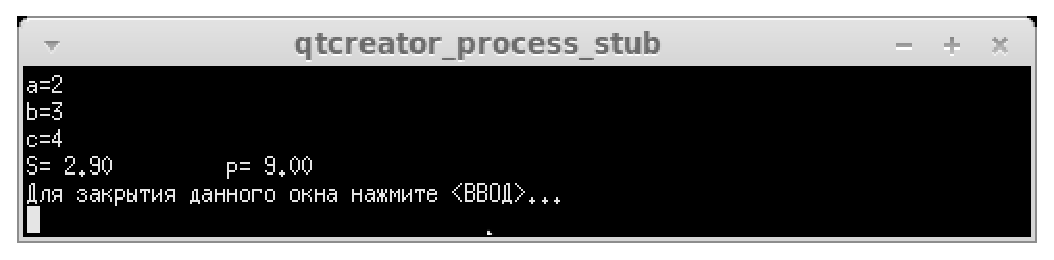
\includegraphics[width=0.7\textwidth]{img/ris_2_7}
\caption{Результаты работы программы к задаче \ref{ch02:prg2} (вариант 1)}
\label{ch02:refDrawing6}
\end{center}
\end{figure}

\begin{lstlisting}
//`ЗАДАЧА~\ref{ch02:prg2}. Вариант второй`
#include <iostream>
#include <stdio.h>
#include <math.h>
using namespace std;
int main()
{
  float a,b,c,S,r;
  printf("Vvedite a, b, c \n");  //`Вывод на экран строки символов.`
  scanf("%f%f%f",&a,&b,&c); //`Ввод значений.`
  r=(a+b+c)/2;
  S=sqrt(r*(r-a)*(r-b)*(r-c));
  printf("S=%5.2f \t p=%5.2f \n",S,2*r); //`Вывод результатов.`
  return 0;
}
\end{lstlisting}

\begin{figure}[htb]
\begin{center}
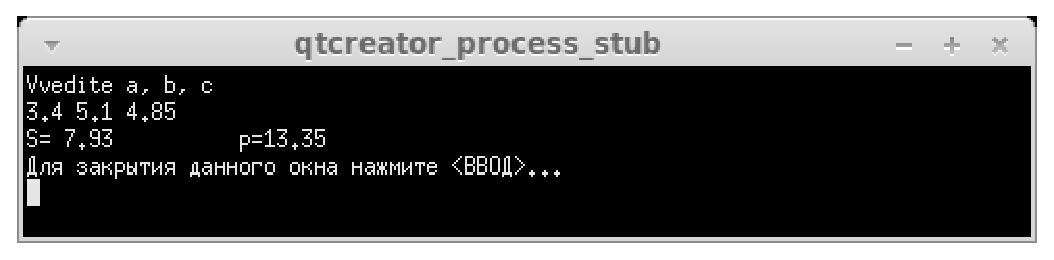
\includegraphics[width=0.7\textwidth]{img/ris_2_8}
\caption{Результаты работы программы к задаче \ref{ch02:prg2} (вариант 2)}
\label{ch02:refDrawing7}
\end{center}
\end{figure}

\subsection[Объектно-ориентированные средства ввода-вывода.]{Объектно-ориентированные средства ввода-вывода.}
Описание объектов для управления вводом-выводом содержится в заголовочном файле \Sys{iostream}. При
подключении этого файла с помощью директивы \Sys{\#include {<}iostream{>}} в программе
автоматически создаются \emph{объекты-потоки}\footnote{Поток --- виртуальный канал связи, создаваемый в
программе для передачи данных} \Sys{cin} для \emph{ввода с клавиатуры} и
\Sys{cout} для \emph{вывода на экран}, а так же операции помещения в поток
\Sys{{<}{<}} и чтения из потока \Sys{{>}{>}}.

Итак, с помощью объекта \Sys{cin} и операции \Sys{{>}{>}} можно ввести
значение любой переменной. Например, если переменная \Sys{i} описана как целочисленная, то команда
\Sys{cin{>}{>} i; }означает, что в переменную \Sys{i} будет записано
некое целое число, введенное с клавиатуры. Если нужно ввести несколько переменных, следует написать
\Sys{cin{>}{>}x{>}{>}y{>}{>}z;}.

Объект \Sys{cout} и операция \Sys{{<}{<}} позволяют вывести на экран значение
любой переменной или текст. Текст необходимо заключать в двойные кавычки, кроме того, допустимо применение специальных
символов \Sys{{\textbackslash}t} и \Sys{{\textbackslash}n} (таблица~\ref{ch02:refTable10}).
Запись \Sys{cout{<}{<}i;} означает вывод на экран значения переменной
$i$. А команда
\Sys{cout{<}{<}x{<}{<}\symbol{`\"}{\textbackslash}t\symbol{`\"}{<}{<}y;} выведет
на экран значения переменных $x$ и $y$ разделенные символом табуляции.

\prg{Дано трехзначное число. Записать его цифры в обратном порядке и вывести на
экран новое число.}{gl2:prg3}

Разберем решение данной задачи на конкретном примере. Здесь будут использоваться операции целочисленной арифметики. 

Пусть \Sys{P=456}. Вычисление остатка от деления числа \Sys{P} на \Sys{10} даст
его последнюю цифру (количество единиц в числе \Sys{P}):
\Sys{456 \% 10 =6.}

Операция деления нацело числа \Sys{P} на \Sys{10} позволит уменьшить количество разрядов и
число станет двузначным:

\Sys{456 / 10 = 45.}

Остаток от деления полученного числа на \Sys{10} будет следующей цифрой числа \Sys{P}
(количество десятков в числе \Sys{P}):

\Sys{45 \% 10 = 5.}

Последнюю цифру числа \Sys{P} (количество сотен) можно найти так:

\Sys{456 / 100 = 4.}

Так как в задаче требовалось записать цифры числа \Sys{P} в обратном порядке, значит в новом числе будет
\Sys{6} сотен, \Sys{5} десятков и \Sys{4} единицы:

\Sys{S = 6*100 + 5*10 + 4 = 654.}

Далее приведен текст программы, реализующей данную задачу для любого трехзначного числа.

\begin{lstlisting}
#include <iostream>
using namespace std;
int main(int argc, char *argv[])
{
unsigned int P, S;  //`Определение целочисленных переменных без знака`.
cout<<"P=";         //`Вывод на экран символов` P=.
cin>>P;             //`Ввод заданного числа` P.
S=P%10*100+P/10%10*10+P/100; //`Вычисление нового числа` S.
cout<<"S="<<S<<endl;         //`Вывод на экран символов` S=` и значения переменной` S.
return 0;
}
\end{lstlisting}

\prg{Пусть целочисленная переменная \Sys{i} и вещественная переменная
\Sys{d} вводятся с клавиатуры. Определить размер памяти, отведенной для хранения этих переменных и их
суммы, в байтах. Вычислить сколько памяти будет выделено для хранения строки \Sys{С Новым Годом!}. Вывести
на экран размеры различных типов данных языка \Sys{С++} в байтах.}{ch02:prg4} 

Далее приведён текст программы.
\begin{lstlisting}
#include <iostream>
using namespace std;
int main()
{
int i;     //`Определение целочисленной переменной`.
double d;  //`Определение вещественной переменной`.

cout<<"i= "; cin>>i;  //`Ввод переменной` i.
cout<<"d= "; cin>>d;  //`Ввод переменной` d.
//`Размер памяти`, `отведенной под переменную` i.
cout<<"`Размер` i: "<<sizeof i<<"\n";
//`Размер памяти, отведенной под переменную` d.
cout<<"`Размер` d: "<<sizeof d<<"\n";
//`Размер памяти, отведенной под значение выражения` i+d.
cout<<"`Размер` i+d: "<<sizeof (i+d)<<"\n";
cout<<"`Размер строки <С Новым Годом!>:`";
//`Размер памяти, отведенной под строку.`
cout<<sizeof "`С Новым годом!`"<<"\n";
//`Вычисление размеров различных типов данных:`
cout<<"`Размер` char: "<<sizeof (char)<<"\n";
cout<<"`Размер` int: "<<sizeof (int)<<"\n";
cout<<"`Размер` short int: "<<sizeof (short int)<<"\n";
cout<<"`Размер` long int: "<<sizeof (long int)<<"\n";
cout<<"`Размер` long long int:";
cout<<sizeof (long long int)<<"\n";
cout<<"`Размер` float: "<<sizeof (float)<<"\n";
cout<<"`Размер` double: "<<sizeof (double)<<"\n";
cout<<"`Размер` long double: "<<sizeof (long double)<<"\n";
return 0;
}
\end{lstlisting}

Результаты работы программы\footnote{Обратите внимание, что при использовании кодировки utf-16 один кириллический символ
занимает в памяти занимает 2 байта.}

\begin{verbatim}
i= 23 
d= 45.76 
Размер i: 4 
Размер d: 8 
Размер i+d: 8 
Размер <С Новым годом!>:26 
Размер char: 1 
Размер int: 4 
Размер short int: 2 
Размер long int: 4 
Размер long long int:8 
Размер float: 4 
Размер double: 8 
Размер long double: 12 
\end{verbatim}

\section[Задачи для самостоятельного решения]{Задачи для самостоятельного решения}
\subsection[Ввод-вывод данных. Операция присваивания.]{Ввод-вывод данных. Операция присваивания.}
Разработать программу на языке \Sys{С++}. Все входные и выходные данные в задачах --- \emph{вещественные числа}.
Для ввода и вывода данных использовать функции \Sys{scanf} и \Sys{printf}.
\begin{enumerate}
\item Даны катеты прямоугольного треугольника $a$ и $b$. Найти гипотенузу
$c$ и углы треугольника ${\alpha}$, ${\beta}$, ${\chi}$.

\item Известна гипотенуза $c$ и прилежащий угол ${\alpha}$ прямоугольного
треугольника. Найти площадь треугольника $S$ и угол~${\beta}$.

\item Известна диагональ квадрата $d$. Вычислить площадь $S$ и периметр
$P$ квадрата.

\item Дан диаметр окружности $d$. Найти ее длину $L$ и площадь круга~$S$.

\item Даны три числа --- $a$, $b$, $c$. Найти их среднее
арифметическое и среднее геометрическое.

\item Даны катеты прямоугольного треугольника $a$ и $b$. Найти его гипотенузу
$c$ и периметр~$P$.

\item Дан длина окружности $L$. Найти ее радиус $R$ и площадь круга~$S$.

\item Даны два ненулевых числа $a$ и $b$. Найти сумму $S$,
разность $R$, произведение $P$ и частное $d$ их квадратов.

\item Поменять местами содержимое переменных $A$ и $B$ и вывести новые значения $A$ и~$B$.

\item Точки $A$ и $B$ заданы координатами на плоскости:
$A(x_1,y_1)$, $B(x_2,y_2)$. Найти длину отрезка $AB$.

\item Заданы два катета прямоугольного треугольника $a$ и $b$. Вычислить его
площадь $S$ и периметр $P$.

\item Даны переменные $A$, $B$, $C$. Изменить их значения,
переместив содержимое $A$ в $B$, $B$ --- в $C$,
$C$ --- в $A$, и вывести новые значения переменных $A$,
$B$, $C$.

\item Известна диагональ ромба $d$. Вычислить его площадь $S$ и периметр
$P$.

\item Найти значение функции  $y=4\cdot (x+1)^{3}+5\cdot (x-1)^{5}+2$ и ее производной при заданном значении
$x$.

\item Даны два ненулевых числа $a$ и $b$. Найти сумму $S$,
разность $R$, произведение $P$ и частное $D$ их модулей.

\item Известны координаты вершин квадрата $ABCD$:
$A(x_1,y_1)$ и $C(x_2,y_2)$. Найти его площадь $S$ и периметр~$P$.

\item Даны длины сторон прямоугольника $a$ и $b$. Найти его площадь
$S$ и периметр~$P$.

\item Известно значение периметра $P$ равностороннего треугольника. Вычислить его площадь~$S$.

\item Задан периметр квадрата $P$. Вычислить сторону квадрата $a$, диагональ
$d$ и площадь~$S$.

\item Дана сторона квадрата $a$. Вычислить периметр квадрата $P$, его площадь
$S$ и длину диагонали~$d$.

\item Три точки заданы координатами на плоскости:
$A(x_1,y_1)$, $B(x_2,y_2)$ и $C(x_3,y_3)$. Найти длины
отрезков $AB$ и $BC$.

\item Даны переменные A, B, C. Изменить их значения, переместив содержимое $A$ в
$C$, $C$ --- в $B$, $B$ --- в
$A$, и вывести новые значения переменных $A$, $B$,
$C$.

\item Даны числа --- $a_1$, $a_2$, $a_3$, $a_4$, $a_5$.
Найти их среднее арифметическое и среднее геометрическое значения.

\item Найти значение функции  $y=\frac{3}{2}\cdot (x+3)^{4}-\frac{1}{5}\cdot (x-1)^{5}$  и ее производной при заданном
значении $x$.

\item Точки $A$ и $B$ заданы координатами в пространстве:
$A(x_1, y_1, z_1)$, $B(x_2, y_2, z_2)$. Найти длину отрезка $AB$.
\end{enumerate}

\subsection[Операции целочисленной арифметики.]{Операции целочисленной арифметики.}
Разработать программу на языке \Sys{С++}. Все входные данные в задачах --- {целые числа}. Для ввода и вывода
данных использовать объектно-ориентированные средства ввода-вывода.

\begin{enumerate}
\item Расстояние $L$ задано в сантиметрах. Найти количество полных метров в нем и остаток в
сантиметрах.
\item Масса $M$ задана в килограммах. Найти количество полных тонн в ней и остаток в килограммах.
\item Дан размер файла $B$в байтах. Найти количество полных килобайтов, которые занимает данный файл
и остаток в байтах.
\item Дано двузначное число. Вывести на экран количество десятков и единиц в нем.
\item Дано двузначное число. Найти сумму его цифр.
\item Дано двузначное число. Найти произведение его цифр.
\item Дано двузначное число. Вывести число, полученное при перестановке цифр исходного числа.
\item Дано трехзначное число. Определить сколько в нем единиц, десятков и сотен.
\item Дано трехзначное число. Найти сумму его цифр.
\item Дано трехзначное число. Найти произведение его цифр.
\item Дано трехзначное число. Вывести число, полученное при перестановке цифр сотен и десятков исходного числа.
\item Дано трехзначное число. Вывести число, полученное при перестановке цифр сотен и единиц исходного числа.
\item Дано трехзначное число. Вывести число, полученное при перестановке цифр десятков и единиц исходного числа.
\item С начала суток прошло N секунд. Найти количество полных минут, прошедших с начала суток и остаток в секндах.
\item С начала суток прошло N секунд. Найти количество полных часов, прошедших с начала суток и остаток в секндах.
\item Дано двузначное число $\alpha\leqslant 88$. Вывести на экран число, которое получится если каждую цифру числа
$a$ увеличить на единицу.
\item Дано двузначное число $\alpha\geqslant 22$. Вывести на экран число, которое получится если каждую цифру числа
$a$ уменьшить на единицу.
\item Расстояние $L$ задано в метрах. Найти количество полных километров в нем и остаток в метрах.
\item Масса $M$ задана в граммах. Найти количество полных килограммов в ней и остаток в граммах.
\item Размер файла $B$ дан в килобайтах. Найти
количество полных мегабайтов, которые занимает данный файл и остаток в килобайтах.
\item Расстояние $L$ задано в дециметрах. Найти количество полных метров в нем и остаток в
сантиметрах.
\item С начала года прошло $K$ дней. Найти количество полных недель, прошедших с начала года и осток в
днях.
\item С начала года прошло $K$ часов. Найти количество полных дней, прошедших с начала года и осток в
часах.
\item Дано двузначное число $a\leqslant 44$. Вывести на экран число, которое получится если удвоить каждую цифру
числа $a$.
\item Дано двузначное число $\alpha\geqslant 22$. Вывести на экран число, которое получится если каждую цифру числа
$a$ уменьшить вдвое.
\end{enumerate}

\subsection[Встроенные математические функции]{Встроенные математические функции}
Разработать программу на языке \Sys{С++}. Все входные и выходные данные в задачах --- \emph{вещественные числа}.
Для ввода и вывода данных использовать функции \Sys{scanf} и \Sys{printf}.

Вычислить значение выражения $y=f(x)$ при заданном значении
$x$. Варианты заданий представлены в таблице~\ref{ch02:refTable11}.

{\noindent\tabcolsep=0.3em\scriptsize
\begin{longtable}{|c|l||c|l|}
\caption{Задачи для самостоятельного решения} \label{ch02:refTable11}\\
\hline
\Emph{№}&\Emph{Выражение $f(x)$}&\Emph{№}&\Emph{Выражение $f(x)$}\\
\hline \hline
\endfirsthead
\multicolumn{4}{c}%
{{\tablename\ \thetable{} --- продолжение}} \\
\hline
\Emph{№}&\Emph{Выражение $f(x)$}&\Emph{№}&\Emph{Выражение $f(x)$}\\
\hline \hline
\endhead
 1 &
$\displaystyle
\sqrt[{7}]{x^2+2.7\cdot \pi \cdot \cos\sqrt{|x^3|}-2}+e^x
$
&%\\\hline
2 &
$\displaystyle
\tg^4x+\sin^2\frac{\pi }{x}-e^{2x^{2}+3.6x-1}
$
\\\hline
3 &
$\displaystyle
\Bigl||x^{4}-\cos x|-\sqrt[{9}]{1+\sqrt{x^{6}}}\Bigr|+\sin ^{3}\frac{\pi }{e^{x}+1}
$
&%\\\hline
4 &
$\displaystyle
\log _4|e^x-4|-\sqrt[{7}]{\left|\frac{2\cdot x}{3.21+\cos ^{2}\frac{\pi }{7}}\right|}
$
\\\hline
5 &
$\displaystyle
\sqrt[{3}]{\sqrt{|x|}}+|\ctg^2x+\frac{e^{x}}{2\cdot \pi }-x^3|
$
&%\\\hline
6 &
$\displaystyle
x^{5}+\log_3^2(3x^{2}+5)+\sqrt[{9}]{(\pi -6x^2)^2}
$
\\\hline
7 &
$\displaystyle
\frac{1-\log|x-\cos (2x-\pi )|}{6+x^{{4x-1}}}+\sqrt[{5}]{x^{3}}
$
&%\\\hline
8 &
$\displaystyle
e^{x+\frac{\pi }{3}}+\sqrt[{3}]{\tg\left|\frac{x^{5}}{x^{2}+13.22}\right|}+\cos^3x
$
\\\hline
9 &
$\displaystyle
x^{1+\frac{3\cdot {\pi }}{4}}-3x^{3}-\sqrt[{5}]{(x+1)^{4}+\lg\left|\frac{x}{x+1}\right|}
$
&%\\\hline
10 &
$\displaystyle
\sqrt[{5}]{x^{3}+\cos \sqrt{\left|{x}^{3}\right|}}+\frac{e^{x}}{\cos (3\cdot x+\frac{\pi }{15})}
$
\\\hline
11 &
$\displaystyle
e^{2x}+\sqrt[{5}]{\ctg\frac{(x-\pi )^{9}}{x^{4}+3.4}}+\sin^{2}6.2x
$
&%\\\hline
12 &
$\displaystyle
\sqrt[{5}]{(x+\tg a)^{2}}-\frac{1-\ln|e^x+\cos \frac{\pi }{8}|}{2}
$
\\\hline
13 &
$\displaystyle
\log (e^{x}+27)-\sqrt{\left|x^{3}+\frac{\sqrt[{5}]{x^{7}}+14}{\sin 5x+5.1\cdot \pi }\right|}
$
&%\\\hline
14 &
$\displaystyle
\ln|\cos (x-2\cdot \pi )|-\sqrt[{3}]{1+\frac{e^x}{\sin x-3}}
$
\\\hline
15 &
$\displaystyle
\sqrt{\left|x^{3}+\frac{\sqrt[{3}]{x^{4}}-1}{\sin x+\pi +e^{x}}\right|}
$
&%\\\hline
16 &
$\displaystyle
\sqrt[{{3}}]{\frac{1+3\cdot \pi }{1+x^{2}}}+|\arctg^2x^3|
$
\\\hline
17 &
$\displaystyle
\tg^2|x|+3^{2x^2-e^x}+\frac{\sqrt[{7}]x^2}{\cos^2{\pi x}}
$
&%\\\hline
18 &
$\displaystyle
x^4-\sqrt[{5}]{\pi -\sqrt{|x^{3}|}+\sin^2\frac{x}{x^{2}+1}}
$
\\\hline
19 &
$\displaystyle
\log (e^{x}+6)-\sqrt[{3}]{(x-4)^{2}+1.47\sin\sqrt{|\pi \cdot x|}}
$
&%\\\hline
20 &
$\displaystyle
\frac{x^5}{\sin |x-7|}+\log^2(x^2+2.5)-\sqrt[{3}]{(\pi -6.1x^2)^2}
$
\\\hline
21 &
$\displaystyle
\ctg^2\frac{x\cdot \pi }{3}-\Bigl(\sqrt{|x|}-3.4\Bigr)^{x^{2}-10}+\ln (x^{2}+3)
$
&%\\\hline
22 &
$\displaystyle
\Biggl|\log_5|x^3-e^x|-\sqrt[3]{\frac{2x}{\cos (x+1.23\cdot \pi )}}\Biggr|
$
\\\hline
23 &
$\displaystyle
\Bigl||\cos \frac{\pi }{7}-e^x|-\sqrt[{7}]{2+\sqrt{x^{5}}}\Bigr|+\ln \frac{x^4+1}{6}
$
&%\\\hline
24 &
$\displaystyle
\log (x^2+2)-\sin ^2x+\sqrt[{5}]{2-\sqrt{|x|}+\sin \frac{\pi }{e^x+1}}
$
\\\hline
25 &
$\displaystyle
\log _2e^x-\cos \frac{x}{\pi }+\sqrt[{3}]{\frac{|\tg (2x)|}{2.6+x^2+x^3}}
$
&&
\\\hline
\end{longtable}
}

\chapter[Операторы управления]{Операторы управления}

В этой главе описаны основные операторы языка \Sys{C++}: условный оператор \Sys{if}, оператор выбора
\Sys{switch}, операторы цикла \Sys{while}, \Sys{do}…\Sys{while} и
\Sys{for}. Изложена методика составления алгоритмов с помощью блок-схем. Приводится большое количество
примеров составления программ различной сложности. 

\section[Основные конструкции алгоритма]{Основные конструкции алгоритма}
При разработке простейших программ несложно перейти от словесного описания к написанию программы. Однако большинство
реально разрабатываемых программ довольно сложные и созданию программы предшествует разработка алгоритма\footnote{От
\emph{algorithmi}, \emph{algorismus}, первоначально латинская транслитерация имени математика
аль-Хорезми.}. \index{Алгоритм}\emph{Алгоритм} --- это чёткое описание последовательности действий, которые
необходимо выполнить, для того чтобы при соответствующих исходных данных получить требуемый результат. Одним из
способов представления алгоритма является \index{Блок-схема}\emph{блок-схема}. При составлении блок-схемы
все этапы решения задачи изображаются с помощью различных геометрических фигур. Эти фигуры называют блоками и, как
правило, сопровождают надписями. Последовательность выполнения этапов указывают при помощи стрелок, соединяющих эти
блоки. Типичные этапы решения задачи изображаются следующими геометрическими фигурами:
\begin{itemize}
\item блок начала-конца (рис. \ref{ch03:refDrawing0}). Надпись внутри блока: «начало» («конец»);

\item блок ввода-вывода данных (рис. \ref{ch03:refDrawing1}). Надпись внутри блока: ввод (вывод или печать) и список вводимых
(выводимых) переменных;

\item блок решения или арифметический (рис. \ref{ch03:refDrawing2}). 
Внутри блока записывается действие, вычислительная операция
или группа операций;

\item условный блок (рис. \ref{ch03:refDrawing3}). Логическое условие записывается внутри блока. В результате проверки условия
осуществляется выбор одного из возможных путей (ветвей) вычислительного процесса. 
\end{itemize}
{\footnotesize
%{\renewcommand{\captiontitlefont}{\footnotesize\sffamily}
   \floatsetup[widefloat]{margins=hangleft,labelfont=footnotesize}
   \begin{figure}%
   \begin{floatrow}[4]
   %\captionnamefont{\footnotesize}
   \ffigbox[\FBwidth]
   {%\captionnamefont{\footnotesize}
   \captionsetup{labelfont=footnotesize}\caption{\footnotesize Блок начала-конца алгоритма}%
   \label{ch03:refDrawing0}}
   {
\includegraphics[width=0.18\textwidth,keepaspectratio]{img/ris_3_1}}%\hspace*{0.01\textwidth}

   \ffigbox[\FBwidth]
   {\caption{\footnotesize Блок ввода-вывода данных}%
   \label{ch03:refDrawing1}}
   {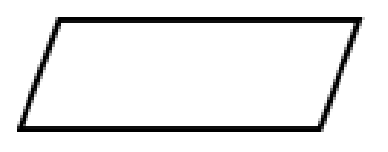
\includegraphics[width=0.18\textwidth,keepaspectratio]{img/ris_3_2}}%\hspace*{0.01\textwidth}

   %\ffigbox[\Xhsize/2]
   \ffigbox[\FBwidth]%[\FBheight][t]
   {\caption{\footnotesize Арифмети\-чёс\-кий блок}%
   \label{ch03:refDrawing2}}
   %{{\setlength\unitlength{\hsize/58}%^^A
   {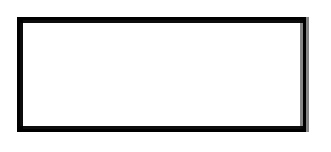
\includegraphics[width=0.18\textwidth,keepaspectratio]{img/ris_3_3}}%\hspace*{0.01\textwidth}
   %}}}
   %\ffigbox[\Xhsize]
   \ffigbox[\FBwidth]%[\FBheight][t]
   {\caption{\footnotesize Условный блок}%
   \label{ch03:refDrawing3}}
   {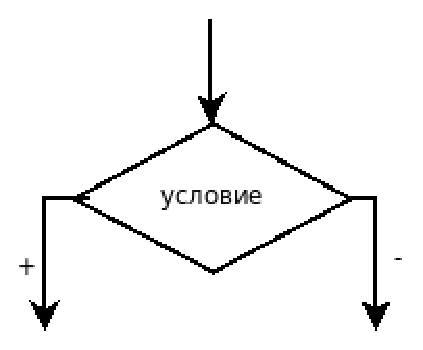
\includegraphics[width=0.31\textwidth,keepaspectratio]{img/ris_3_4}}%}
   \end{floatrow}
   \end{figure}%
}

Рассмотренные блоки позволяют описать три \index{Алгоритм!основные конструкции}\emph{основные конструкции
алгоритма}: линейный процесс, разветвляющийся процесс и циклический процесс.

\index{Алгоритм!линейный}\emph{Линейный процесс} это конструкция, представляющая собой последовательное
выполнение двух или более операторов (рис.~\ref{ch03:refDrawing4}).
\index{Алгоритм!разветвляющийся}\emph{Разветвляющийся процесс} задаёт выполнение одного или другого
оператора в зависимости от выполнения условия (рис.~\ref{ch03:refDrawing5}).
\index{Алгоритм!циклический}\emph{Циклический процесс} задаёт многократное выполнение оператора или группы
операторов (рис.~\ref{ch03:refDrawing6}).

{\footnotesize
%{\renewcommand{\captionnamefont}{\footnotesize\sffamily}
   \floatsetup[widefloat]{margins=hangleft}
   \begin{figure}%
   \begin{floatrow}[3]
   \captionnamefont{\footnotesize}
   \ffigbox[\FBwidth]
   {\captionnamefont{\footnotesize}\caption{\footnotesize Ли\-ней\-ный процесс}%
   \label{ch03:refDrawing4}}
   {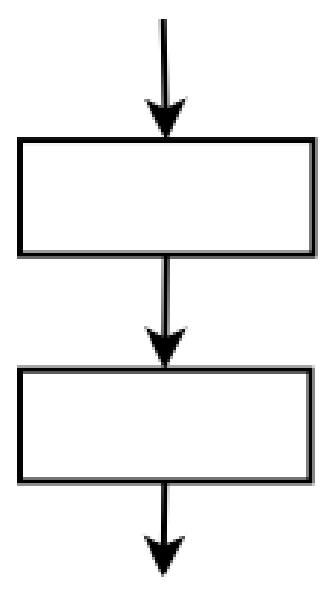
\includegraphics[width=0.18\textwidth,keepaspectratio]{img/ris_3_5}}%\hspace*{0.01\textwidth}

   %\ffigbox[\Xhsize/2]
   \ffigbox[\FBwidth]%[\FBheight][t]
   {\caption{\footnotesize Разветвляющийся процесс}%
   \label{ch03:refDrawing5}}
   %{{\setlength\unitlength{\hsize/58}%^^A
   {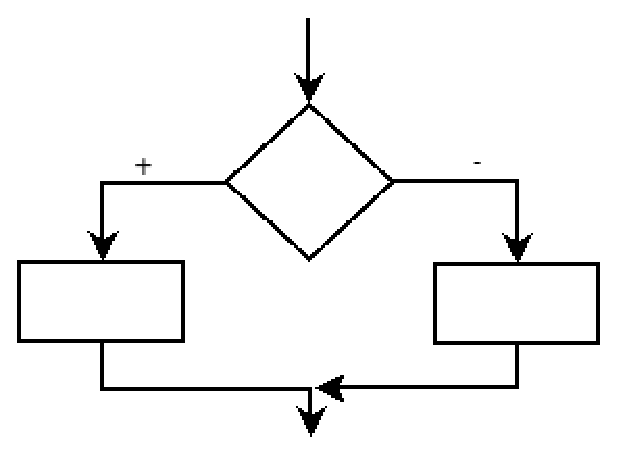
\includegraphics[width=0.42\textwidth,keepaspectratio]{img/ris_3_6}}%\hspace*{0.01\textwidth}
   %}}}
   %\ffigbox[\Xhsize]
   \ffigbox[\FBwidth]%[\FBheight][t]
   {\caption{\footnotesize Циклический процесс}%
   \label{ch03:refDrawing6}}
   {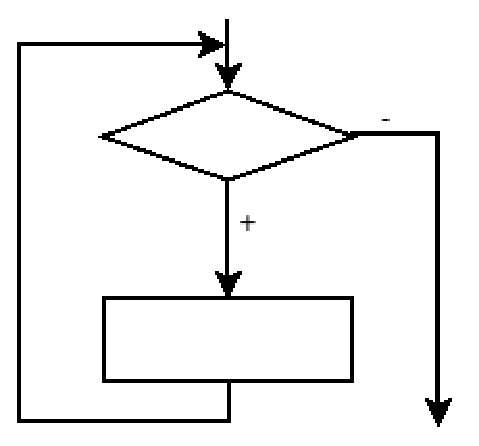
\includegraphics[width=0.32\textwidth,keepaspectratio]{img/ris_3_7}}%}
   \end{floatrow}
   \end{figure}%
%\renewcommand{\captionnamefont}{\small\sffamily}
}

Нетрудно заметить, что каждая из основных конструкций алгоритма имеет один вход и один выход. Это позволяет вкладывать
конструкции друг в друга произвольным образом и составлять алгоритмы для решения задач любой сложности.

Одним из важных понятий при написании программ на \Sys{С}(\Sys{С++}) является понятие составного оператора.

\section[Составной оператор]{Составной оператор}
\index{Оператор!составной}\emph{Составной оператор} --- это группа операторов, отделённых друг от друга
точкой с запятой, начинающихся с открывающей фигурной скобки \{ и заканчивающихся закрывающейся
фигурной скобкой \}:
\begin{lstlisting}
{
  `\Sys{оператор\_1;}`
  `\Sys{...}`
  `\Sys{оператор\_n;}`
}
\end{lstlisting}

Транслятор воспринимает составной оператор как одно целое.

Рассмотрим операторы языка \Sys{С++}, реализующие основные конструкции алгоритма.

\section[Условные операторы]{Условные операторы}
Одна из основных конструкций алгоритма --- 
\index{Оператор!разветвляющийся}\emph{разветвляющийся процесс}. Он реализован в языке
\Sys{С++} двумя условными операторами: \Sys{if} и \Sys{switch}. Рассмотрим каждый из них.

\subsection[Условный оператор]{Условный оператор}
При решении большинства задач порядок вычислений зависит от определённых условий, например, от исходных данных или от
промежуточных результатов, полученных на предыдущих шагах программы. Для организации вычислений в зависимости от
какого-либо условия в \Sys{С++} предусмотрен \index{Оператор!условный}\emph{условный оператор} \Sys{if}, 
который в общем виде записывается следующим образом:
\begin{lstlisting}
if `\Sys{(условие) оператор\_1}`; else `\Sys{оператор\_2}`;
\end{lstlisting}
где \Sys{условие} --- это логическое (или целое) выражение, переменная или константа, 
\Sys{оператор\_1} и \Sys{оператор\_2} --- любой оператор языка \Sys{С(С++)}.

Работает условный оператор следующим образом. Сначала вычисляется значение выражения, указанного в скобках. Если
оно не равно нулю, т.е. имеет значение истина (\Sys{true}), выполняется \Sys{оператор\_1}. В
противном случае, когда выражение равно нулю, т.е. имеет значение ложь (\Sys{false}), выполняется
\Sys{оператор\_2}. Алгоритм, который реализован в условном операторе \Sys{if}, представлен на
рис.~\ref{ch03:refDrawing7}.

%\begin{figure}[htb]
%\begin{center}
%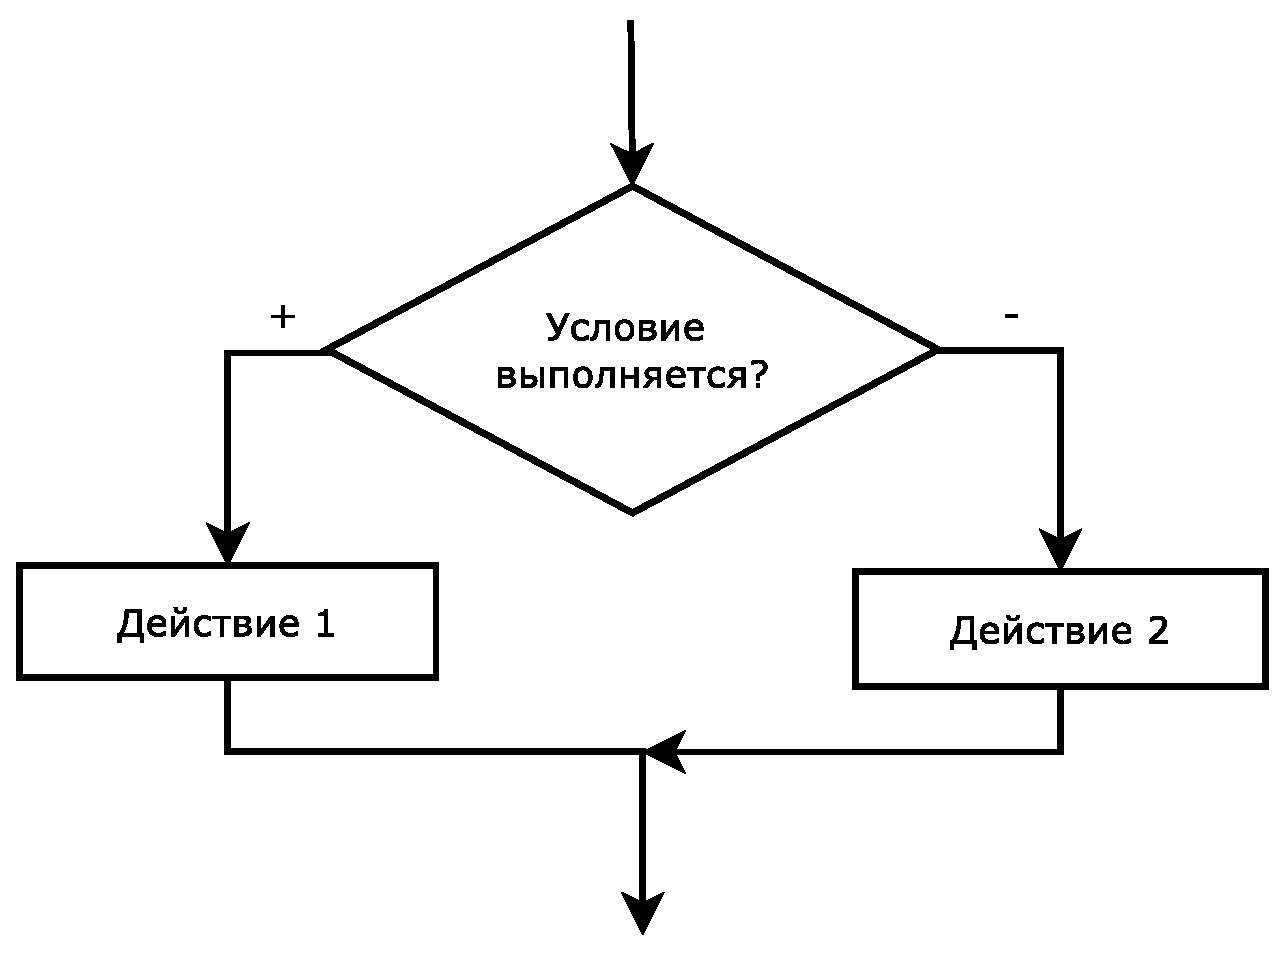
\includegraphics[width=0.5\textwidth]{img/ris_3_8}
%\caption{Алгоритм условного оператора \Sys{if … else}}
%\label{ch03:refDrawing7}
%\end{center}
%\end{figure}

Например, чтобы сравнить значения переменных \Sys{a} и \Sys{b} нужно написать следующий
программный код:
\begin{lstlisting}
cin>>a; cin>>b;
if (a==b) cout<<"a `\Sys{равно}` b";
else cout<<"a `\Sys{не равно}` b";
\end{lstlisting}

\Emph{Внимание!} Не путайте знак проверки равенства \Sys{==} и оператор присваивания
\Sys{=}. Например, в записи \Sys{if (a=0) b=1;} синтаксической ошибки нет. Операция
присваивания \Sys{a=0} формирует результат и его значение проверяется в качестве условия. В данном примере
присваивание \Sys{b=1} не будет выполнено никогда, так как переменная \Sys{a} всегда будет
принимать значение равное нулю, то есть ложь. Верная запись: 
\Sys{if (a==0) b=1;}.

%%%% рис 8 и 9 бок о бок
\begin{figure}[H]
\begin{floatrow}
\floatbox{figure}[.45\textwidth][\FBheight][t]
{\caption{Алгоритм условного оператора \Sys{if … else}}
\label{ch03:refDrawing7}}
{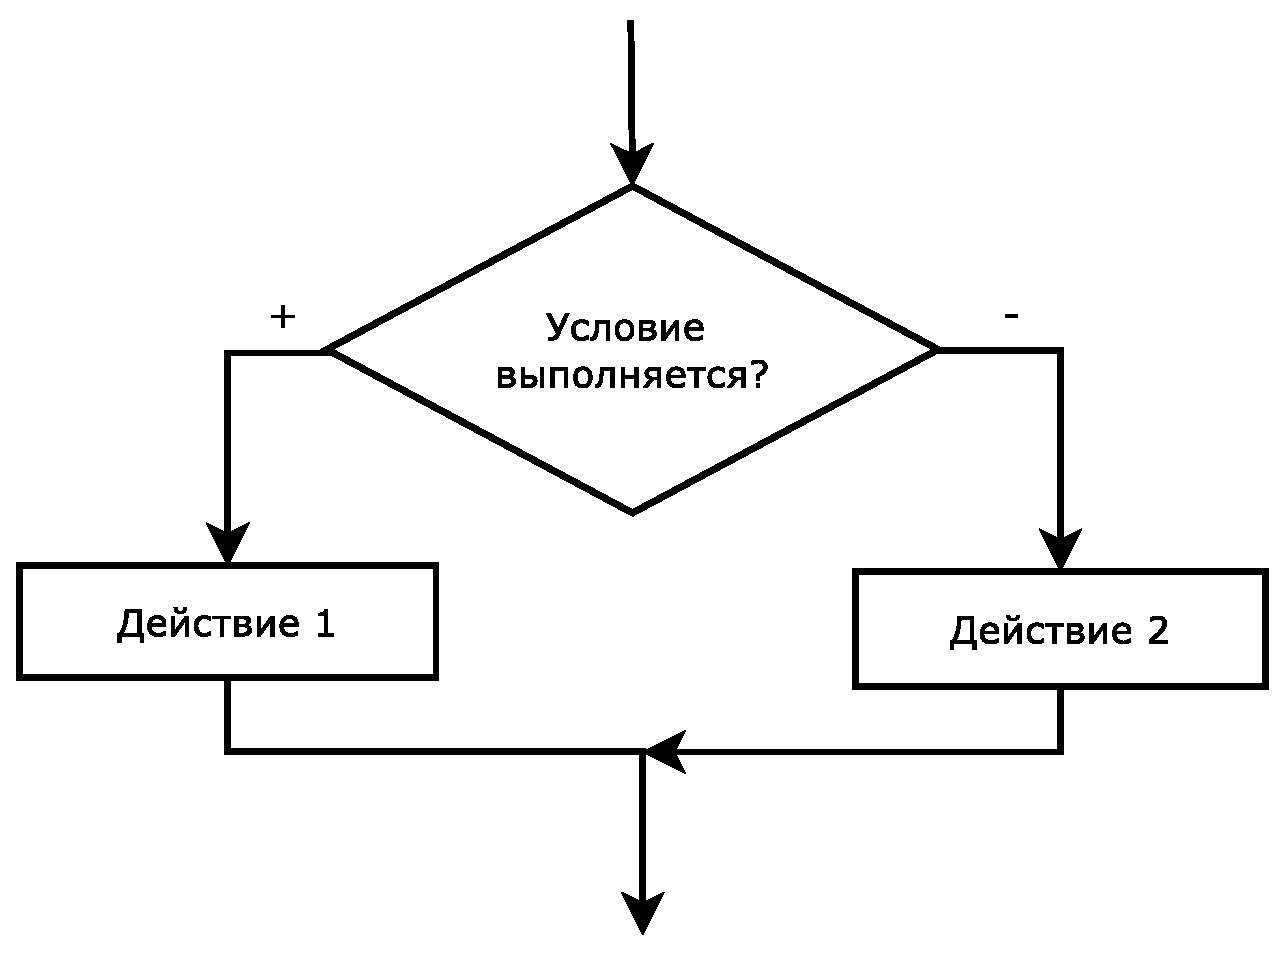
\includegraphics[width=0.45\textwidth,keepaspectratio]{img/ris_3_8}}\hspace*{0.05\textwidth}
%
\floatbox{figure}[.45\textwidth][\FBheight][b]
{\caption{Алгоритм условного оператора \Sys{if}}
\label{ch03:refDrawing8}}
{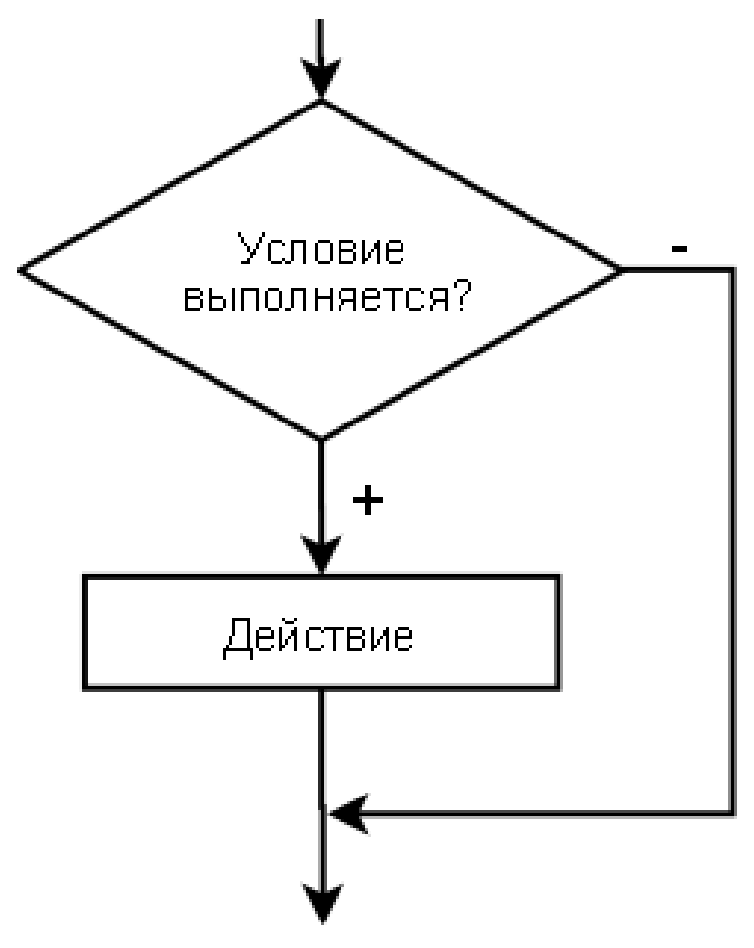
\includegraphics[width=0.35\textwidth]{img/ris_3_9}}
\end{floatrow}
\end{figure}

\Emph{Внимание!} Если в задаче требуется, чтобы в зависимости от значения условия выполнялся не один оператор, а
несколько, их необходимо заключать в фигурные скобки, как составной оператор. В этом случае компилятор воспримет группу
операторов как один:
\begin{lstlisting}
if (`\Sys{условие}`) 
{
  `\Sys{оператор\_1;}`
  `\Sys{оператор\_2;}`
    `…`
}
else 
{
  `\Sys{оператор\_3;}`
  `\Sys{оператор\_4;}`
    `…`
}
\end{lstlisting}

Альтернативная ветвь \Sys{else} в условном операторе может отсутствовать, если в ней нет необходимости: 
\begin{lstlisting}
if (`\Sys{условие}`) `\Sys{оператор;}`
\end{lstlisting}
или
\begin{lstlisting}
if (`\Sys{условие}`)
{
  `\Sys{оператор\_1;}`
  `\Sys{оператор\_2;}`
  `\Sys{…}`
}
\end{lstlisting}

В таком <<усечённом>> виде условный оператор работает так: \Sys{оператор} (группа операторов) либо
выполняется, либо пропускается, в зависимости от значения выражения, представляющего условие. Алгоритм этого условного
процесса представлен на рис.~\ref{ch03:refDrawing8}.


%\begin{figure}[htb]
%\begin{center}
%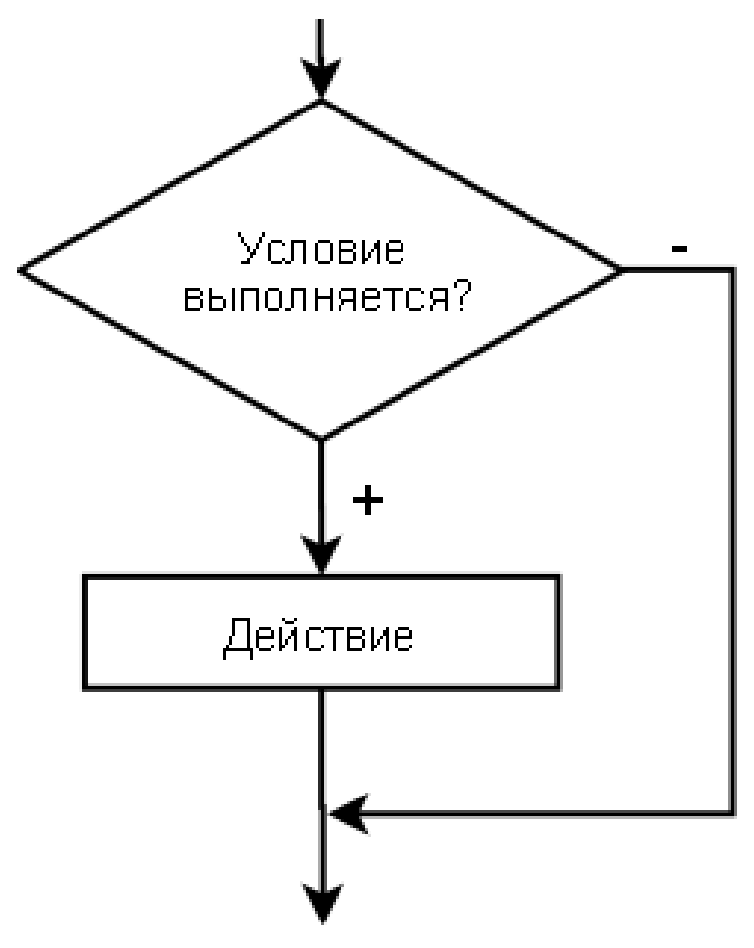
\includegraphics[width=0.5\textwidth]{img/ris_3_9}
%\caption{Алгоритм условного оператора \Sys{if}}
%\label{ch03:refDrawing8}
%\end{center}
%\end{figure}

Пример применения условного оператора без альтернативной ветви \Sys{else} может быть таким:

\begin{lstlisting}
cin>>a; cin>>b;
c=0;
//`Значение переменной \Sys{c} изменяется только при условии, что \Sys{a} не равно \Sys{b}`
if (a!=b) c=a+b;
cout<<"c="<<c;
\end{lstlisting}

Условные операторы могут быть вложены друг в друга. При вложениях условных операторов всегда действует правило:
альтернатива \Sys{else} считается принадлежащей ближайшему \Sys{if}. Например, в записи
\begin{lstlisting}
if `(условие\_1)` if `(условие\_2) оператор\_А`; else `оператор\_Б;`
\end{lstlisting}
\Sys{оператор\_Б} относится к \Sys{условию\_2}, а в конструкции
\begin{lstlisting}
if `(условие\_1)` {if `(условие\_2) оператор\_А`;} 
else `оператор\_Б;`
\end{lstlisting}
он принадлежит оператору \Sys{if} с \Sys{условием\_1}. 

Рассмотрим несколько задач с применением условных процессов.

\prg{Дано вещественное число $x$. Для
функции, график которой приведён на рис.~\ref{ch03:refDrawing9}, вычислить
$y=f(x)$.}{ch03:prg0}

\begin{figure}[htb]
\begin{center}
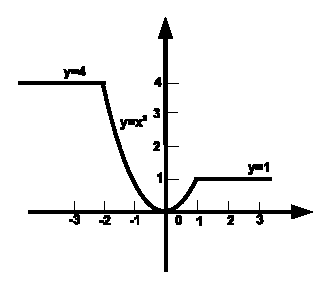
\includegraphics[width=0.5\textwidth]{img/ris_3_10}
\caption{Графическое представление задачи \ref{ch03:prg0}}
\label{ch03:refDrawing9}
\end{center}
\end{figure}

Аналитически функцию, представленную на рис.~\ref{ch03:refDrawing9}, можно записать так:

\begin{equation*}
y(x)=\left\{\begin{matrix}
4, & x\leqslant -2\\
1, & x\geqslant 1\\
x^2, & -2<x<1
\end{matrix}\right.
\end{equation*}

Составим словесный алгоритм решения этой задачи:

\begin{enumerate}
\item Начало алгоритма.
\item Ввод числа $x$ (аргумент функции).
\item Если значение $x$ меньше либо равно -2, то переход к п.~4, иначе переход к~п.~5.
\item Вычисление значения функции: $y=4$, переход к~п.~8.
\item Если значение $x$ больше либо равно 1, то переход к п.~6, иначе переход к~п.~7.
\item Вычисление значения функции: $y=1$, переход к~п.~8.
\item Вычисление значения функции: $y=x^2$.
\item Вывод значений аргумента $x$ и функции $y$.
\item Конец алгоритма.
\end{enumerate}

Блок-схема, соответствующая описанному алгоритму, представлена на рис.~\ref{ch03:refDrawing10}.

\begin{figure}[htb]
\begin{center}
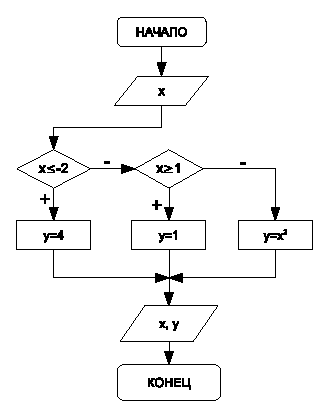
\includegraphics[width=0.5\textwidth]{img/ris_3_11}
\caption{Блок-схема алгоритма решения задачи~\ref{ch03:prg0}}
\label{ch03:refDrawing10}
\end{center}
\end{figure}

Текст программы на языке \Sys{C++} будет иметь вид:
\begin{lstlisting}
#include <iostream>
using namespace std;
int main()
{
  float X,Y;
  cout<<"X="; cin>>X;
  if (X<=-2) Y=4;
  else if (X>=1) Y=1;
  else Y=X*X;
  cout <<"Y=" <<Y<< endl;
  return 0;
}
\end{lstlisting}

\prg{Даны вещественные числа $x$ и $y$. Определить, принадлежит ли точка с координатами ($x$; $y$)
заштрихованной области (рис.~\ref{ch03:refDrawing11}).}{ch03:prg1}

%\begin{figure}[htb]
%\begin{center}
%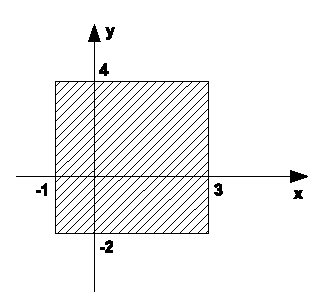
\includegraphics[width=0.3\textwidth]{img/ris_3_12}
%\caption{Графическое представление задачи~\ref{ch03:prg1}}
%\label{ch03:refDrawing11}
%\end{center}
%\end{figure}

%%%% рис 12 и 13 бок о бок
\begin{figure}[H]
\begin{floatrow}
\floatbox{figure}[.35\textwidth][\FBheight][t]
{\caption{Графическое представление задачи~\ref{ch03:prg1}}
\label{ch03:refDrawing11}}
{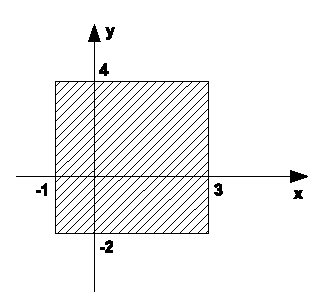
\includegraphics[width=0.3\textwidth,keepaspectratio]{img/ris_3_12}}\hspace*{0.05\textwidth}
%
\floatbox{figure}[.45\textwidth][\FBheight][b]
{\caption{Алгоритм решения задачи~\ref{ch03:prg1}}
\label{ch03:refDrawing12}}
{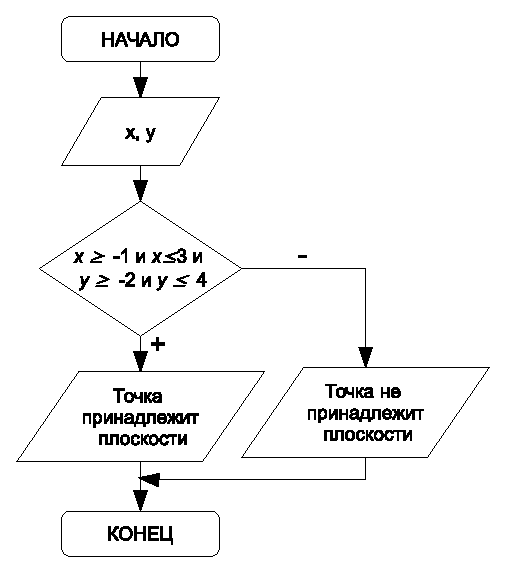
\includegraphics[width=0.4\textwidth]{img/ris_3_13}}
\end{floatrow}
\end{figure}


Как показано на рис.~\ref{ch03:refDrawing11}, область ограничена линиями $x=-1$, $x=3$,
$y=-2$ и $y=4$. Значит точка с координатами ($x$;
$y$) будет принадлежать этой области, если будут выполняться следующие условия: 
$x\geqslant -1$, $x\leqslant 3$, $y\geqslant -2$ и $y\leqslant 4$. Иначе точка лежит за пределами области.

Блок-схема, описывающая алгоритм решения данной задачи, представлена на рис.~\ref{ch03:refDrawing12}.

%\begin{figure}[htb]
%\begin{center}
%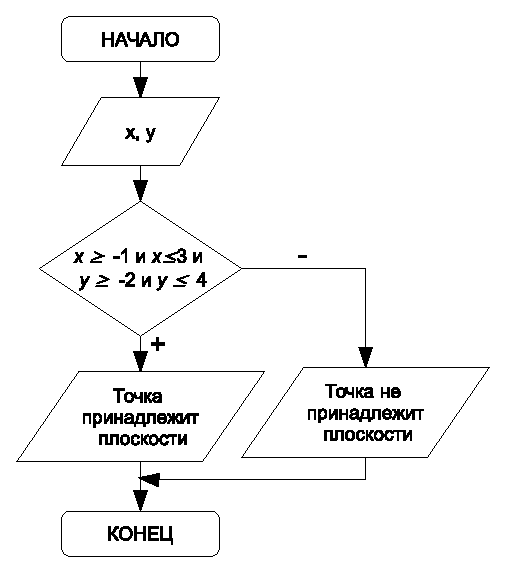
\includegraphics[width=0.4\textwidth]{img/ris_3_13}
%\caption{Алгоритм решения задачи~\ref{ch03:prg1}}
%\label{ch03:refDrawing12}
%\end{center}
%\end{figure}

Текст программы к задаче~\ref{ch03:prg1}:
\begin{lstlisting}
#include <iostream>
using namespace std;
int main()
{float X,Y;
cout<<"X="; cin>>X;
cout<<"Y="; cin>>Y;
if (X>=-1 && X<=3 && Y>=-2 && Y<=4)
  cout <<"`\Sys{Точка принадлежит области}`"<< endl;
else 
  cout<<"`\Sys{Точка не принадлежит области}`"<<endl;
return 0;
}
\end{lstlisting}

\prg{Даны вещественные числа $x$ и $y$. Определить, принадлежит ли точка с координатами ($x$; $y$)
заштрихованной области (рис.~\ref{ch03:refDrawing13}).}{ch03:prg3}

\begin{figure}[htb]
\begin{center}
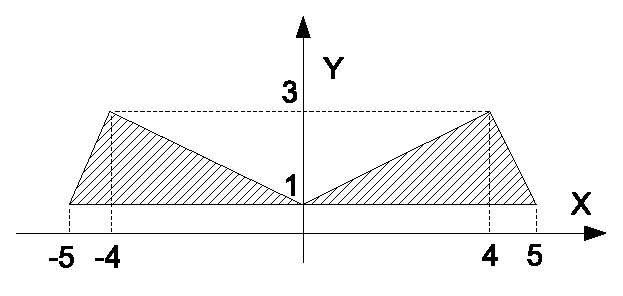
\includegraphics[width=0.5\textwidth]{img/ris_3_14}
\caption{Графическое представление задачи~\ref{ch03:prg3}}
\label{ch03:refDrawing13}
\end{center}
\end{figure}

Составим уравнения линий, ограничивающих заданные области. В общем виде уравнение прямой, проходящей через точки с
координатами  $(x_1,y_1)$ и  $(x_2,y_2)$,  имеет вид:

 $$\frac{x-x_1}{x_2-x_1}=\frac{y-y_1}{y_2-y_1}$$.

Треугольник в первой координатной области ограничен линиями, проходящими через точки:

\begin{enumerate}
\item $(0, 1) - (4, 3)$;
\item $(4, 3) - (5, 1)$;
\item $(5, 1) - (0, 1)$.
\end{enumerate}
Следовательно, уравнение первой линии:

 $$\frac{x-0}{4-0}=\frac{y-1}{3-1}\Rightarrow \frac{x}{4}=\frac{y-1}{2}\Rightarrow y=1+\frac{1}{2}\cdot x,$$
уравнение второй линии:
$$
\frac{x-4}{5-4}=\frac{y-3}{1-3}\Rightarrow x-4=\frac{y-3}{-2}\Rightarrow -2\cdot x+8=y-3\Rightarrow y=-2\cdot x+11
$$
и уравнение третьей линии:  $y=1$.

Линии, которые формируют треугольник во второй координатной области, проходят через точки:

\begin{enumerate}
\item $(0, 1) - (-4, 3)$;
\item $(-4, 3) - (-5, 1)$;
\item $(-5, 1) - (0, 1)$;
\end{enumerate}
Следовательно, уравнение первой линии:
 $$\frac{x-0}{-4-0}=\frac{y-1}{3-1}\Rightarrow \frac{x}{-4}=\frac{y-1}{2}\Rightarrow y=1-\frac{1}{2}\cdot x,$$
уравнение второй линии:
$$
\frac{x+4}{-5+4}=\frac{y-3}{1-3}\Rightarrow \frac{x+4}{-1}=\frac{y-3}{-2}\Rightarrow -2\cdot x-8=-y+3\Rightarrow
y=2\cdot x+11
$$
и уравнение третьей линии:  $y=1$.

Таким образом, условие попадания точки в заштрихованную часть плоскости имеет вид:

\begin{equation*}
\left\{
\begin{array}{c}
y\leqslant 1+\frac{1}{2}\cdot x\\
y\leqslant -2\cdot x+11\\
y\geqslant 1
\end{array}%
\right.
\ \ \text{или}\ \  
\left\{
\begin{array}{c}
y\leqslant 1-\frac{1}{2}\cdot x\\
y\leqslant 2\cdot x+11\\
y\geqslant 1
\end{array}
\right. 
\end{equation*}

Далее приведён текст программы для решения задачи \ref{ch03:prg3}.

\begin{lstlisting}
#include <iostream>
using namespace std;
int main()
{
	float X,Y;
	cout<<"X=";
	cin>>X;
	cout<<"Y=";
	cin>>Y;
	if ((Y<=1+(float)1/2*X && Y<=-2*X+11 && Y>=1) || (Y<=1-(float)1/2*X && Y<=2*X+11 && Y>=1))
		cout <<`\Sys{"Точка принадлежит области"}`<< endl;
	else
		cout<<`\Sys{"Точка не принадлежит области"}`<< endl;
	return 0;
}
\end{lstlisting}

\prg{Написать программу решения квадратного уравнения\\
$ax^2+bx+c=0$.}{ch03:prg4} 

Исходные данные: вещественные числа $a$, $b$ и $c$ --- коэффициенты
квадратного уравнения.

Результаты работы программы: вещественные числа $x1$ и $x2$ --- корни квадратного
уравнения либо сообщение о том, что корней нет.

Вспомогательные переменные: вещественная переменная $d$, в которой будет храниться дискриминант
квадратного уравнения.

Составим словесный алгоритм решения этой задачи.
\begin{enumerate}
\item Начало алгоритма.
\item Ввод числовых значений переменных $a$, $b$ и $c$.
\item Вычисление значения дискриминанта $d$ по формуле  $d=b^2-4ac$.
\item Если $d<0$, то переход к п.5, иначе переход к п.6.
\item Вывод сообщения \Sys{"Действительных корней нет"} и переход к п.8.
\item Вычисление корней  $x1=\frac{-b+\sqrt{d}}{2a}$  и  $x2=\frac{-b-\sqrt{d}}{2a}$.
\item Вывод значений $x1$ и $x2$ на экран.
\item Конец алгоритма.
\end{enumerate}
Блок-схема, соответствующая этому описанию, представлена на рис.~\ref{ch03:refDrawing14}.

\begin{figure}[htb]
\begin{center}
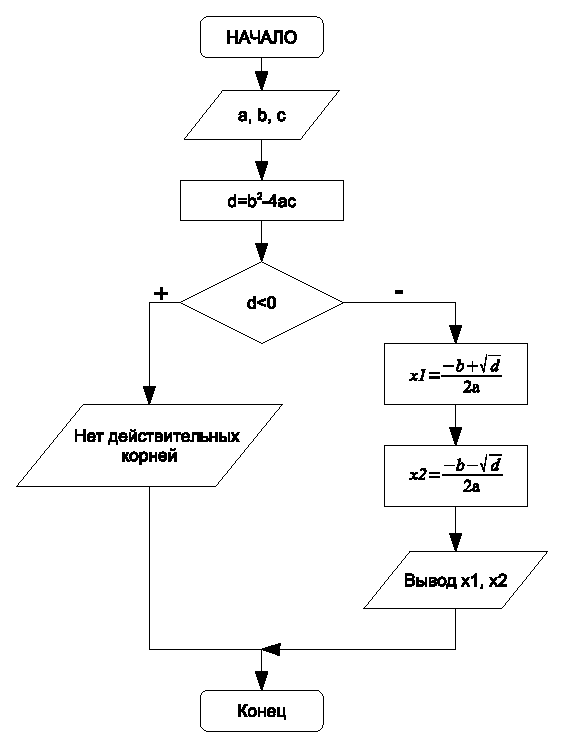
\includegraphics[width=0.7\textwidth]{img/ris_3_15}
\caption{Алгоритм решения квадратного уравнения}
\label{ch03:refDrawing14}
\end{center}
\end{figure}

Текст программы, которая реализует решение квадратного уравнения: 
\begin{lstlisting}
#include <iostream>
#include <math.h>
using namespace std;
int main()
{
float a,b,c,d,x1,x2;
//`Ввод значений коэффициентов квадратного уравнения.`
cout<<"a=";cin>>a;
cout<<"b=";cin>>b;
cout<<"c=";cin>>c;
d=b*b-4*a*c;	//`\Sys{Вычисление дискриминанта.}`
if (d<0)        
//`Если дискриминант отрицательный, то вывод сообщения, о том что действительных корней нет,`
  cout<<"`\Sys{Нет действительных корней}`";
else
{
//`иначе вычисление действительных корней`
  x1=(-b+sqrt(d))/2/a;
  x2=(-b-sqrt(d))/(2*a);
//`и вывод их значений.`
  cout<<"X1="<<x1<<"\t X2="<<x2<<"\n";
}
return 0;
}
\end{lstlisting}

\prg{Составить программу нахождения действительных и
комплексных корней квадратного уравнения
$ax^2+bx+c=0$.}{ch03:prg5} 

Исходные данные: вещественные числа $a$, $b$ и $c$ --- коэффициенты
квадратного уравнения.

Результаты работы программы: вещественные числа $x1$ и $x2$ --- действительные корни
квадратного уравнения либо $x1$ и $x2$ --- действительная и мнимая части комплексных
корней квадратного уравнения.

Вспомогательные переменные: вещественная переменная $d$, в которой будет храниться дискриминант
квадратного уравнения.

Можно выделить следующие этапы решения задачи:
\begin{enumerate}
\item Ввод коэффициентов квадратного уравнения $a$, $b$ и $c$.
\item Вычисление дискриминанта $d$ по формуле  $d=b^2-4ac$.
\item Проверка знака дискриминанта. Если $d\geqslant 0$, то вычисление действительных корней:
 $x1=\frac{-b+\sqrt{d}}{2a}$  и  $x2=\frac{-b-\sqrt{d}}{2a}$ 
и вывод их на экран. При отрицательном дискриминанте выводится сообщение о том, что действительных корней нет, и
вычисляются комплексные корни\footnote{Комплексные числа записываются в виде
$a+ib$, где $a$ --- действительная часть комплексного числа,
$b$ --- мнимая часть комплексного числа, $i$ --- мнимая единица  $\sqrt{-1}$. Подробно о комплексных числах можно прочитать в главе~\ref{ch09}.}
 $x1=\frac{-b}{2a}+i\frac{\sqrt{\left|{d}\right|}}{2a}$, 
$x2=\frac{-b}{2a}-i\frac{\sqrt{\left|{d}\right|}}{2a}$.
\end{enumerate}

У обоих комплексных корней действительные части одинаковые, а мнимые отличаются знаком. Поэтому можно в переменной
$x1$ хранить действительную часть числа  $\frac{-b}{2a}$, в переменной $x2$ --- модуль мнимой части 
$\frac{\sqrt{\left|{d}\right|}}{2a}$, а в качестве корней вывести 
$x1 + i\cdot x2$  и  $x1 - i\cdot x2$. 

На рис.~\ref{ch03:refDrawing15} изображена блок-схема решения задачи. Блок~1 предназначен для ввода коэффициентов квадратного
уравнения. В блоке~2 осуществляется вычисление дискриминанта. Блок~3 осуществляет проверку знака дискриминанта, если
дискриминант отрицателен, то корни комплексные, их расчёт происходит в блоке~4 (действительная часть корня записывается
в переменную $x1$, модуль мнимой --- в переменную $x2$), а вывод --- в блоке~5 (первый
корень $x1 + i\cdot x2$, второй --- $x1 - i\cdot x2$). Если дискриминант положителен, то
вычисляются действительные корни уравнения (блок~6) и выводятся на экран (блок~7).

\begin{figure}[htb]
\begin{center}
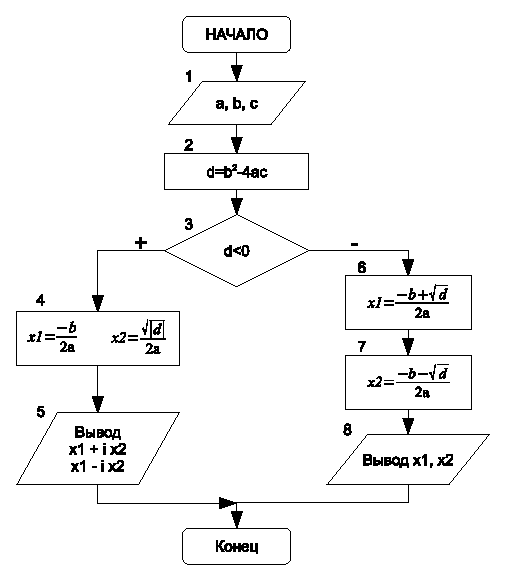
\includegraphics[width=0.7\textwidth]{img/ris_3_16}
\caption{Алгоритм решения задачи \ref{ch03:prg5}}
\label{ch03:refDrawing15}
\end{center}
\end{figure}

Текст программы, реализующей поставленную задачу:
\begin{lstlisting}
#include <iostream>
#include <math.h>
using namespace std;
int main()
{
float a,b,c,d,x1,x2;
cout<<"a=";cin>>a;
cout<<"b=";cin>>b;
cout<<"c=";cin>>c;
d=b*b-4*a*c;
if (d<0)
{//`\Sys{Если дискриминант отрицательный, то вывод соответствующего сообщения.}`
  cout<<"`\Sys{Нет вещественных корней }`\n";
  x1=-b/(2*a);  //`\Sys{Вычисление действительной части комплексных корней.}`
  x2=sqrt(fabs(d))/(2*a); //`\Sys{Вычисление модуля мнимой части комплексных корней}`
  //`\Sys{Сообщение о комплексных корнях уравнения вида} $ax^2+bx+c=0$.`
  cout<<"`\Sys{Комплексные корни уравнения}` \n";
  cout<<a<<"x^2+"<<b<<"x+"<<c<<"=0 \n";
  //`\Sys{Вывод значений комплексных корней в виде $x1\pm ix2$}`
  if (x2>=0)
  {
    cout<<x1<<"+"<<x2<<"i\t";
    cout<<x1<<"-"<<x2<<"i\n";
  }
  else
  {
    cout<<x1<<"-"<<fabs(x2)<<"i\t";
    cout<<x1<<"+"<<fabs(x2)<<"i\n";
  }
}
else
{
//`\Sys{Если дискриминант положительный, вычисление действительных корней и вывод их на экран.}`
  x1=(-b+sqrt(d))/2/a;
  x2=(-b-sqrt(d))/(2*a);
  cout<<"`\Sys{Вещественные корни уравнения}` \n";
  cout<<a<<"x^2+"<<b<<"x+"<<c<<"=0 \n";
  cout<<"X1="<<x1<<"\t X2="<<x2<<"\n";
}
return 0;
}
\end{lstlisting}

Результаты работы программы к задаче~\ref{ch03:prg5} показаны ниже.%рис. \ref{ch03:refDrawing16} и \ref{ch03:refDrawing17}.
\begin{verbatim}
a=-5
b=-3
c=-4
Нет вещественных корней 
Комплексные корни уравнения 
-5x^2+-3x+-4=0 
-0.3-0.842615i	-0.3+0.842615i
==============================
a=2
b=-3
c=1
Вещественные корни уравнения 
2x^2+-3x+1=0 
X1=1	 X2=0.5
\end{verbatim}


\prg{Составить программу для решения кубического уравнения\\
$ax^3+bx^2+cx+d=0$.}{ch03:prg6}

Кубическое уравнение имеет вид
\begin{equation}\label{ch03:eq1}
ax^3+bx^2+cx+d=0
\end{equation}

После деления на $a$ уравнение~\ref{ch03:eq1} принимает канонический вид:
\begin{equation}\label{ch03:eq2}
x^{3}+rx^2+sx+t=0,
\end{equation}
где $r=\frac{b}{a}$, $s=\frac{c}{a}$, $t=\frac{d}{a}$. 

В уравнении~\ref{ch03:eq2} сделаем замену  $x=y-\frac{r}{3}$  и получим приведённое уравнение:
\begin{equation}\label{ch03:eq3}
y^3+py+q=0,
\end{equation}
где $p=\frac{3s-r^2}{3}$,  $q=\frac{2r^3}{27}-\frac{rs}{3}+t$.

Число действительных корней приведённого уравнения (\ref{ch03:eq3}) зависит от знака дискриминанта (табл.
\ref{ch03:refTable0})
 $D=(\frac{p}{3})^3+(\frac{q}{2})^2$.

{\tabcolsep=0.3em\noindent\small
\begin{longtable}{|p{0.2\textwidth}|p{0.33\textwidth}|p{0.35\textwidth}|}
\caption{Количество корней кубического уравнения} \label{ch03:refTable0}\\
\hline
\Emph{Дискрими\-нант}&\Emph{Количество действительных корней}&\Emph{Количество комплексных корней}\\
\hline \hline
\endfirsthead
\multicolumn{3}{c}%
{{\tablename\ \thetable{} --- продолжение}} \\
\hline
\Emph{Дискрими\-нант}&\Emph{Количество действительных корней}&\Emph{Количество комплексных корней}\\
\hline \hline
\endhead
\centering $D\geqslant 0$ & \centering 1 & \centering 2\tabularnewline\hline
\centering $D<0$ & \centering 3 & \centering\ $-$\tabularnewline\hline
\end{longtable}
}

Корни приведённого уравнения могут быть рассчитаны по формулам Кардано:

\begin{equation}\label{ch03:eq4}
\begin{array}{l}
y_1=u+v\\
y_2=\frac{-{u+v}}{2}+\frac{u-v}{2}i\sqrt{3}\\
y_3=\frac{-{u+v}}{2}-\frac{u-v}{2}i\sqrt{3},
\end{array}
\end{equation}
где $u=\sqrt[{3}]{\frac{-q}{2}+\sqrt{D}}$,\ \  $v=\sqrt[{3}]{\frac{-q}{2}-\sqrt{D}}$.

При отрицательном дискриминанте уравнение (\ref{ch03:eq1}) имеет три действительных корня, но они будут вычисляться
через вспомогательные комплексные величины. Чтобы избавиться от этого, можно воспользоваться формулами:
\begin{equation}\label{ch03:eq5}
\begin{array}{l}
y_1=2\sqrt[{3}]{\rho}\cos(\frac{\phi}{3}),\\
y_2=2\sqrt[{3}]{\rho}\cos(\frac{\phi}{3}+\frac{2\pi}{3}),\\
y_3=2\sqrt[{3}]{\rho}\cos(\frac{\phi}{3}+\frac{4\pi}{3}),
\end{array}
\end{equation}
где $\rho =\sqrt{\frac{-{p^{3}}}{27}},\ \ \cos(\phi )=\frac{-{q}}{2\rho}$.

Таким образом, при положительном дискриминанте кубического уравнения (\ref{ch03:eq3}) расчёт корней будем вести по
формулам (\ref{ch03:eq4}), а при отрицательном --- по формулам (\ref{ch03:eq5}). После расчёта корней приведённого
уравнения (\ref{ch03:eq3}) по формулам (\ref{ch03:eq4}) или (\ref{ch03:eq5}), необходимо по формулам 

\begin{equation*}
x_{k}=y_{k}-\frac{r}{3},\ k=1,2,3..,
\end{equation*}
перейти к корням заданного кубического уравнения (\ref{ch03:eq1}).

Блок-схема решения кубического уравнения представлена на рис.~\ref{ch03:refDrawing19}.

\begin{figure}[ht]
\begin{center}
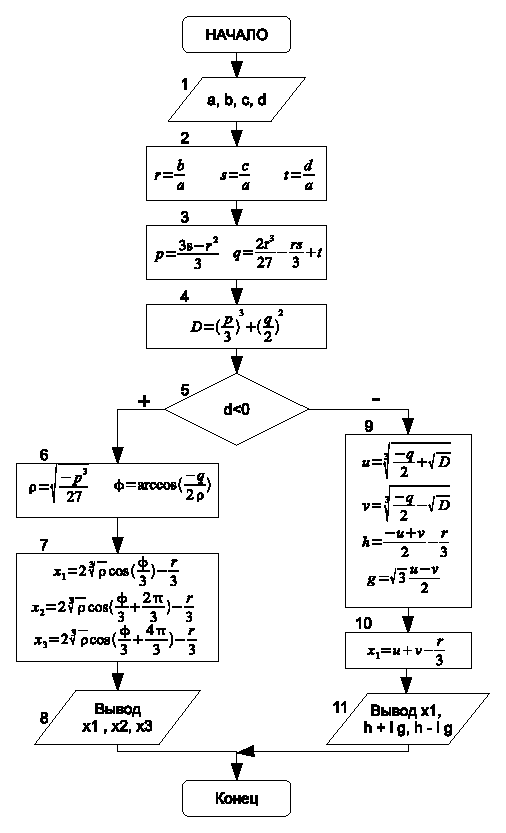
\includegraphics[width=0.6\textwidth]{img/ris_3_19}
\caption{Алгоритм решения кубического уравнения}
\label{ch03:refDrawing18}
\end{center}
\end{figure}

Описание блок-схемы. В блоке 1 вводятся коэффициенты кубического уравнения, в блоках 2--3 рассчитываются коэффициенты
канонического и приведённого уравнений. Блок 4 предназначен для вычисления дискриминанта. В блоке 5 проверяется знак
дискриминанта кубического уравнения. Если он отрицателен, то корни вычисляются по формулам~\ref{ch03:eq5} (блоки 6--7). При
положительном значении дискриминанта расчёт идёт по формулам~\ref{ch03:eq4} (блок 9, 10). Блоки 8 и 11 предназначены для вывода результатов на экран.

Текст программы с комментариями приведён ниже\footnote{При расчёте величин \Sys{u} и \Sys{v} в
программе предусмотрена проверка значения подкоренного выражения. 

Если  $\frac{-q}{2}\mp\sqrt{D}>0$,\ \ то\ \ $u=\sqrt[{3}]{\frac{-q}{2}+\sqrt{D}}$, 
а \ \ $v=\sqrt[{3}]{\frac{-q}{2}-\sqrt{D}}$.

Если  $\frac{-q}{2}\mp\sqrt{D}<0$,\ \ то\ \ $u=\sqrt[{3}]{|\frac{-q}{2}+\sqrt{D}|}$,
\ \  а\ \ $v=\sqrt[{3}]{|\frac{-q}{2}-\sqrt{D}|}$.

Соответственно, при нулевом значении подкоренного выражения \Sys{u} и \Sys{v} обращаются
в ноль}.

\begin{lstlisting}
#include <iostream>
#include <math.h>
using namespace std;
#define pi 3.14159  //`\Sys{Определение константы}`
int main()
{
float a,b,c,d,D,r,s,t,p,q,ro,fi,x1,x2,x3,u,v,h,g;
//`\Sys{Ввод коэффициентов кубического уравнения.}`
cout<<"a="; cin>>a;
cout<<"b="; cin>>b;
cout<<"c="; cin>>c;
cout<<"d="; cin>>d;
//`\Sys{Расчёт коэффициентов канонического уравнения по формуле~\ref{ch03:eq2}}`
r=b/a; s=c/a; t=d/a;
//`\Sys{Вычисление коэффициентов приведённого уравнения по формуле~\ref{ch03:eq3}}`
p=(3*s-r*r)/3; q=2*r*r*r/27-r*s/3+t;
//`\Sys{Вычисление дискриминанта кубического уравнения}`
D=(p/3)*(p/3)*(p/3)+(q/2)*(q/2);
if (D<0)
{
  //`\Sys{Формулы ~\ref{ch03:eq5}}`
  ro=sqrt((float)(-p*p*p/27));
  fi=-q/(2*ro);
  fi=pi/2-atan(fi/sqrt(1-fi*fi));
  x1=2*pow(ro,(float)1/3)*cos(fi/3)-r/3;
  x2=2*pow(ro,(float)1/3)*cos(fi/3+2*pi/3)-r/3;
  x3=2*pow(ro,(float)1/3)*cos(fi/3+4*pi/3)-r/3;
  cout<<"\n x1="<<x1<<"\t x2="<<x2;
  cout<<"\t x3="<<x3<<"\n";
}
else
{
  //`\Sys{Формулы ~\ref{ch03:eq4}}`
  if (-q/2+sqrt(D)>0) u=pow((-q/2+sqrt(D)),(float)1/3);
  else 
  if (-q/2+sqrt(D)<0) u=-pow(fabs(-q/2+sqrt(D)),(float)1/3);
  else u=0;
  if (-q/2-sqrt(D)>0) v=pow((-q/2-sqrt(D)),(float)1/3);
  else
  if (-q/2-sqrt(D)<0) v=-pow(fabs(-q/2-sqrt(D)),(float)1/3);
  else v=0;
    x1=u+v-r/3; //`\Sys{Вычисление действительного корня кубического уравнения.}`
    h=-(u+v)/2-r/3; //`\Sys{Вычисление действительной}` 
    g=(u-v)/2*sqrt((float)3); //`\Sys{и мнимой части комплексных корней}`
    cout<<"\n x1="<<x1;
    if (x2>=0)
      {
        cout<<x1<<"+"<<x2<<"i\t";
        cout<<x1<<"-"<<x2<<"i\n";
      }
    else
      {
        cout<<x1<<"-"<<fabs(x2)<<"i\t";
        cout<<x1<<"+"<<fabs(x2)<<"i\n";
      }
    }
if (g>=0)
{
cout<<"\t x2="<<h<<"+"<<g<<"i";
cout<<"\t x3="<<h<<"-"<<g<<"i \n";
}
else
{
cout<<"\t x2="<<h<<"-"<<fabs(g)<<"i";
cout<<"\t x2="<<h<<"+"<<fabs(g)<<"i";
}
}
return 0;
}
\end{lstlisting}


\prg{Заданы коэффициенты $a$, $b$ и $c$ биквадратного уравнения
$ax^4+bx^2+c=0$. Найти все его действительные корни.}{ch03:prg7}

\emph{Входные данные}: $a$, $b$, $c$.

\emph{Выходные данные}: $x1$, $x2$, $x3$, $x4$.

Для решения биквадратного уравнения необходимо заменой $y=x^2$
привести его к квадратному уравнению
$ay^2+by+c=0$ и решить это уравнение.

Опишем алгоритм решения этой задачи (рис.~\ref{ch03:refDrawing19}):
\begin{enumerate}
\item Ввод коэффициентов биквадратного уравнения $a$, $b$ и $c$ (блок~1).
\item Вычисление дискриминанта уравнения $d$ (блок~2).
\item Если $d<0$ (блок~3), вывод сообщения, что корней нет (блок~4), а иначе определяются
корни соответствующего квадратного уравнения $y1$ и $y2$ (блок~5).
\item Если $y1<0$ и $y2<0$ (блок~6) , то вывод сообщения, что корней нет (блок~7).
\item Если $y1\geq 0$ и $y2\geq 0$ (блок~8), то вычисляются четыре корня по формулам  
$\pm\sqrt{y_1}, \pm\sqrt{y_2}$ (блок~9) и выводятся значения корней (блок~10).
\item Если условия 4) и 5) не выполняются, то необходимо проверить знак $y1$. Если
$y1\geq 0$ (блок~11), то вычисляются два корня по формуле  $\pm\sqrt{y_1}$ (блок~12), 
иначе (если  $y2\geq 0$) вычисляются два корня по формуле  $\pm\sqrt{y_2}$ (блок~13). Вывод вычисленных
значений корней (блок 14).
\end{enumerate}

\begin{figure}[ht]
\begin{center}
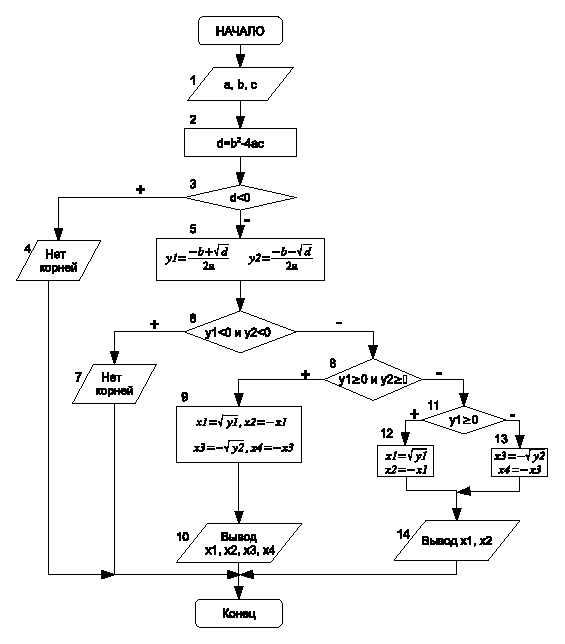
\includegraphics[width=0.7\textwidth]{img/ris_3_20}
\caption{Алгоритм решения биквадратного уравнения}
\label{ch03:refDrawing19}
\end{center}
\end{figure}

Текст программы решения биквадратного уравнения приведён ниже.

\Emph{Внимание!} Если в условном операторе проверяется двойное условие, необходимо применять логические операции
\Sys{{\textbar}{\textbar}}, \Sys{\&\&}, \Sys{!}. Например, условие «если
$y1$ и $y2$ положительны» правильно записать так: \Sys{if (y1{\textgreater}=0 \&\& y2{\textgreater}=0)}.
\begin{lstlisting}
#include <iostream>
#include <math.h>
using namespace std;

int main()
{//`Описание переменных:`
 //a,b,c - `коэффициенты биквадратного уравнения,`
 //d - `дискриминант,`
 //x1,x2,x3,x4 - `корни биквадратного уравнения,`
 //y1,y2 - `корни квадратного уравнения` ay^2+by+c=0,
 float a,b,c,d,x1,x2,x3,x4,y1,y2;
 //`Ввод коэффициентов уравнения.`
 cout<<"a="; cin>>a;
 cout<<"b="; cin>>b;
 cout<<"c="; cin>>c;
 d=b*b-4*a*c;  //`Вычисление дискриминанта.`
 if (d<0)  //`Если дискриминант отрицательный, вывод сообщения «Корней нет».`
  cout<<"`Нет действительных корней` \n";
 else  //`Если дискриминант положительный`,
 {
 //`Вычисление корней соответствующего квадратного уравнения`.
   y1=(-b+sqrt(d))/2/a;
   y2=(-b-sqrt(d))/(2*a);
 //`Если оба корня квадратного уравнения отрицательные`,
  if (y1<0 && y2<0)
 //`вывод сообщения «Корней нет»`
     cout<<" `Нет действительных корней` \n";
 //`Если оба корня квадратного уравнения положительные`,
   else if (y1>=0 && y2>=0)
   {//`Вычисление четырёх корней биквадратного уравнения`
    x1=sqrt(y1);
    x2=-x1;
    x3=sqrt(y2);
    x4=-sqrt(y2);
    //`Вывод корней уравнения на экран`.
    cout<<"\t X1="<<x1<<"\t X2="<<x2;
    cout<<"\t X3="<<x3<<"\t X4="<<x4<<"\n";
   }
    //`Если не выполнились условия`
    //1. y1<0 `и` y2<0
    //2. y1>=0 `и` y2>=0,
    //`то проверяем условие` y1>=0.
    else if (y1>=0) //`Если оно истинно`
    { //`вычисляем два корня биквадратного уравнения.`
      x1=sqrt(y1);
      x2=-x1;
      cout<<"X1="<<x1<<"\t X2="<<x2<<"\n";
    }
    else
    { //`Если условие` y1>=0 `ложно, то вычисляем два корня биквадратного уравнения`
      x1=sqrt(y2);
      x2=-x1;
      cout<<"X1="<<x1<<"\t X2="<<x2<<"\n";
    }
  }
return 0;
}
\end{lstlisting}



Читателю предлагается самостоятельно модифицировать программу таким образом, чтобы она находила все корни (как
действительные, так и комплексные) биквадратного уравнения.

\subsection[Оператор варианта]{Оператор варианта}
Оператор варианта \Sys{switch} необходим в тех случаях, когда в зависимости от значений какой-либо
переменной надо выполнить те или иные операторы:
\begin{lstlisting}
switch `\Sys{(выражение)}`
{
case `\Sys{значение\_1: Операторы\_1;}` break;
case `\Sys{значение\_2: Операторы\_2;}` break;
case `\Sys{значение\_3: Операторы\_3;}` break;
  `\Sys{…}`
case `\Sys{значение\_n: Операторы\_n;}` break;
default: `\Sys{Операторы;}` break;
}
\end{lstlisting}

Оператор работает следующим образом. Вычисляется значение выражения (оно должно быть целочисленным). 
Если выражение принимает
\Sys{значение\_1}, то выполняются \Sys{операторы\_1}. Если выражение принимает
\Sys{значение\_2}, то выполняется \Sys{операторы\_2} и так далее. Если выражение не принимает
ни одно из значений, то выполняются операторы, расположенные после ключевого слова \Sys{default}.

Альтернативная ветвь \Sys{default} может отсутствовать, тогда оператор имеет вид:
\begin{lstlisting}
switch `\Sys{(выражение)}`
{
case `\Sys{значение\_1: Операторы\_1;}` break;
case `\Sys{значение\_2: Операторы\_2;}` break;
case `\Sys{значение\_3: Операторы\_3;}` break;
  `\Sys{…}`
case `\Sys{значение\_n: Операторы\_n;}` break;
}
\end{lstlisting}

Оператор \Sys{break} необходим для того, чтобы осуществить выход из оператора \Sys{switch}.
Если оператор \Sys{break} не указан, то будут выполняться следующие операторы из списка, несмотря на то,
что значение, которым они помечены, не совпадает со значением выражения.

Рассмотрим применение оператора варианта.

\prg{Вывести на печать название дня недели, соответствующее
заданному числу $D$, при условии, что в месяце 31 день и 1-е число --- понедельник.}{ch03:prg8}

Для решения задачи воспользуемся операцией \Sys{\%}, позволяющей вычислить остаток от деления двух чисел,
и условием, что 1-е число --- понедельник. Если в результате остаток от деления (обозначим его $R$)
заданного числа $D$ на семь будет равен единице, то это понедельник, двойке --- вторник, тройке --- среда
и так далее. Следовательно, при построении алгоритма необходимо использовать семь условных операторов, как показано
рис.~\ref{ch03:refDrawing20}. Решение задачи станет значительно проще, если при написании 
программы воспользоваться оператором
варианта \Sys{switch}:
\begin{lstlisting}
#include <iostream>
using namespace std;
int main()
{unsigned int D,R; //`Описаны целые положительные числа.`
  cout<<"D="; cin>>D;  //`Ввод числа от 1 до 31.`
  R=D%7;
  switch (R)
  {
    case 1: cout<<"`Понедельник` \n"; break;
    case 2: cout<<"`Вторник` \n"; break;
    case 3: cout<<"`Среда` \n"; break;
    case 4: cout<<"`Четверг` \n"; break;
    case 5: cout<<"`Пятница` \n"; break;
    case 6: cout<<"`Суббота` \n"; break;
    case 0: cout<<"`Воскресенье` \n"; break;
  }
return 0;
}
\end{lstlisting}
\begin{figure}[htb]
\begin{center}
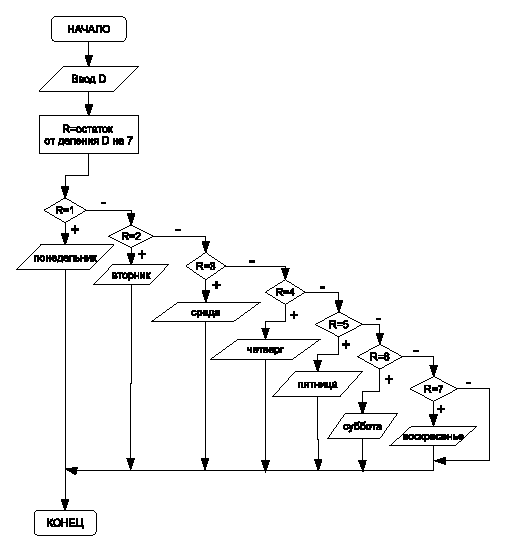
\includegraphics[width=0.7\textwidth]{img/ris_3_21}
\caption{Алгоритм решения задачи \ref{ch03:prg8}}
\label{ch03:refDrawing20}
\end{center}
\end{figure}

В предложенной записи оператора варианта отсутствует ветвь \Sys{default}. Это объясняется тем, что
переменная $R$ может принимать только одно из указанных значений, т.е. 1, 2, 3, 4, 5, 6 или 0. Однако
программа будет работать неправильно, если пользователь введёт значение $D$, превышающее 31. Чтобы
избежать подобной ошибки лучше сделать дополнительную проверку входных данных:
\begin{lstlisting}
#include <iostream>
using namespace std;
int main()
{
unsigned int D,R;
cout<<"\n D="; cin>>D;
if (D<32)  //`Проверка введённого значения.`
{
  R=D%7;
  switch (R)
  {
    case 1: cout<<"`Понедельник` \n"; break;
    case 2: cout<<"`Вторник` \n"; break;
    case 3: cout<<"`Среда` \n"; break;
    case 4: cout<<"`Четверг` \n"; break;
    case 5: cout<<"`Пятница` \n"; break;
    case 6: cout<<"`Суббота` \n"; break;
    case 0: cout<<"`Воскресенье` \n"; break;
  }
}
//`Сообщение об ошибке в случае некорректного ввода.`
else cout<<"`ОШИБКА!` \n";
return 0;
}
\end{lstlisting}

\prg{По заданному номеру месяца $m$ вывести на экран его 
название.}{ch03:prg9}

Для решения данной задачи необходимо проверить выполнение двенадцати условий. 
Если $m$ равно единице, то это январь, если двойке, то февраль, тройке --- март и так далее. 
Понятно, что область возможных значений переменной $m$
находится в диапазоне от 1 до 12 и если пользователь введёт число не входящее в этот интервал, то появится сообщение об
ошибке.
\begin{lstlisting}
#include <iostream>
using namespace std;
int main()
{
  unsigned int m;  //`Описано целое положительное число.`
  cout<<"m="; cin>>m;
  switch (m)
  {
//`В зависимости от значения` m `выводится название месяца.`
    case 1: cout<<"`Январь` \n"; break;
    case 2: cout<<"`Февраль` \n"; break;
    case 3: cout<<"`Март` \n"; break;
    case 4: cout<<"`Апрель` \n"; break;
    case 5: cout<<"`Май` \n"; break;
    case 6: cout<<"`Июнь` \n"; break;
    case 7: cout<<"`Июль` \n"; break;
    case 8: cout<<"`Август` \n"; break;
    case 9: cout<<"`Сентябрь` \n"; break;
    case 10:cout<<"`Октябрь` \n"; break;
    case 11:cout<<"`Ноябрь` \n"; break;
    case 12:cout<<"`Декабрь` \n"; break;
//`Если значение переменной` m `выходит за пределы области`
//`допустимых значений, то выдаётся сообщение.`
    default: cout<<"`ОШИБКА!` \n"; break;
  }
return 0;
}
\end{lstlisting}

\section[Операторы цикла]{Операторы цикла}
\index{Оператор!циклический}\emph{Циклический процесс} или просто
\index{Алгоритм!циклический}\emph{цикл}  это повторение одних и тех же действий. Последовательность
действий, которые повторяются в цикле, называют \emph{телом цикла}. Один проход цикла называют
\emph{шагом} или \emph{итерацией}. Переменные, которые изменяются внутри цикла и влияют на
его окончание, называются \emph{параметрами цикла}. 

При написании циклических алгоритмов следует помнить следующее. Во-первых, чтобы цикл имел шанс когда-нибудь
закончиться, содержимое его тела должно обязательно влиять на условие цикла. Во-вторых, условие должно состоять из
корректных выражений и значений, определённых ещё до первого выполнения тела цикла. 

В \Sys{С++} для удобства пользователя предусмотрены три оператора, реализующих циклический процесс: \Sys{while},
\Sys{do…while} и \Sys{for}.

\subsection[Оператор цикла с предусловием]{Оператор цикла с предусловием}
На рис.~\ref{ch03:refDrawing21} изображена блок-схема алгоритма \index{Алгоритм!цикл с предусловием}\index{Оператор!цикл с
предусловием}\emph{цикла с предусловием}. Оператор, реализующий этот алгоритм в \Sys{С++}, имеет вид:
\begin{lstlisting}
while `\Sys{(условие) оператор;}`
\end{lstlisting}
здесь \Sys{условие} --- логическое или целочисленное выражение, \Sys{оператор} --- любой оператор языка \Sys{С(С++)}.

\begin{figure}[htb]
\begin{center}
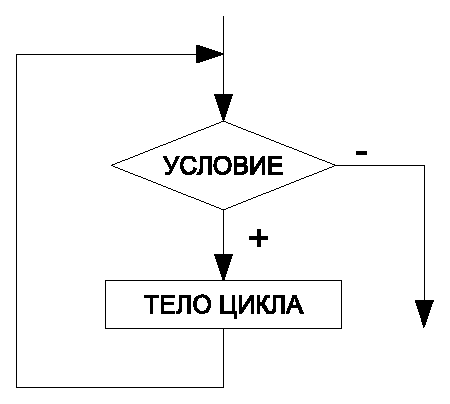
\includegraphics[width=0.3\textwidth]{img/ris_3_22}
\caption{Алгоритм циклической структуры с предусловием}
\label{ch03:refDrawing21}
\end{center}
\end{figure}

Работает цикл с предусловием следующим образом. Вычисляется \Sys{условие}. Если оно истинно (не равно
нулю), то выполняется \Sys{оператор}, и \Sys{условие} проверяется вновь. В противном случае цикл заканчивается, и управление передаётся
оператору, следующему за телом цикла. Условие вычисляется перед каждой итерацией цикла. Если при первой проверке
выражение равно нулю, цикл не выполнится ни разу. Тип выражения должен быть арифметическим или приводимым к нему. 

Если тело цикла состоит более чем из одного оператора, необходимо использовать составной оператор:
\begin{lstlisting}
while `\Sys{(условие)}`
{
  `\Sys{оператор 1;}`
  `\Sys{оператор 2;}`
  `\Sys{…}`
  `\Sys{оператор n;}`
}
\end{lstlisting}

Рассмотрим пример. Пусть необходимо вывести на экран таблицу значений функции  $y=e^{\sin (x)}\cos (x)$ на отрезке 
$[0;\pi]$ с шагом 0.1. Применив \emph{цикл с предусловием}, получим:
%\label{ch03:out0}
\begin{lstlisting}
#include <stdio.h>
#include <math.h>
#define PI 3.14159
using namespace std;
int main()
{
float x, y; //`Описание переменных`
x=0;        //`Присваивание параметру цикла стартового значения`
//`Цикл с предусловием`
while (x<=PI)	//`Пока параметр цикла не превышает конечное значение`
{ //`выполнять тело цикла`
  y=exp(sin(x))*cos(x); //`Вычислить значение` y
  //`Вывод на экран пары` x `и` y.
  printf("\t x=%5.2f \t y=%5.4f \n",x,y);
  x+=0.1;  //`Изменение параметра цикла` 
  //(`переход к следующему значению` x)
} //`Конец цикла`
return 0;
}
\end{lstlisting}

В результате работы данного фрагмента программы на экран последовательно будут выводиться сообщения со значениями
переменных $x$ и $y$\label{ch03:out0}:% (рис.~\ref{ch03:refDrawing22}).

\smallskip
\noindent%\begin{figure}[h]
\begin{minipage}{.3\textwidth}
\begin{verbatim}
x= 1.00      y=1.2534 
x= 1.10      y=1.1059 
x= 1.20      y=0.9203 
x= 1.30      y=0.7011 
x= 1.40      y=0.4553 
x= 1.50      y=0.1918 
x= 1.60      y=-0.0793 
x= 1.70      y=-0.3473 
x= 1.80      y=-0.6017 
x= 1.90      y=-0.8328 
x= 2.00      y=-1.0331
\end{verbatim}
\end{minipage}
%\hspace*{0.05\textwidth}
\begin{minipage}{.3\textwidth}
\begin{verbatim}
x= 2.10      y=-1.1969 
x= 2.20      y=-1.3209 
x= 2.30      y=-1.4045 
x= 2.40      y=-1.4489 
x= 2.50      y=-1.4576 
x= 2.60      y=-1.4348 
x= 2.70      y=-1.3862 
x= 2.80      y=-1.3172 
x= 2.90      y=-1.2334 
x= 3.00      y=-1.1400 
x= 3.10      y=-1.0416 
\end{verbatim}
\end{minipage}
\hfill
%\end{figure}

\subsection[Оператор цикла с постусловием]{Оператор цикла с постусловием}
В цикле с предусловием предварительной проверкой определяется, выполнять тело цикла или нет, до первой итерации. Если
это не соответствует логике алгоритма, то можно использовать \index{Оператор!цикл с постусловием}
\index{Алгоритм!цикл с постусловием}\emph{цикл с постусловием}. На рис.~\ref{ch03:refDrawing23}
видно, что в этом цикле проверяется, делать или нет очередную итерацию, лишь после завершения предыдущей. Это имеет
принципиальное значение лишь на первом шаге, а далее циклы ведут себя идентично. 

\begin{figure}[htb]
\begin{center}
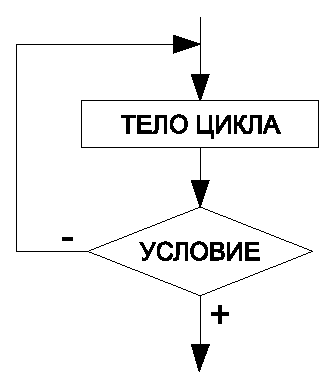
\includegraphics[width=0.3\textwidth]{img/ris_3_24}
\caption{Алгоритм циклической структуры с постусловием}
\label{ch03:refDrawing23}
\end{center}
\end{figure}

В \Sys{С++} \emph{цикл с постусловием} реализован конструкцией
\begin{lstlisting}
do `\Sys{оператор}` while `\Sys{(условие)}`;
\end{lstlisting}
здесь \Sys{условие} --- логическое или целочисленное выражение, 
\Sys{оператор} --- любой оператор языка С(С++). Если тело 
цикла состоит более чем из одного оператора:
\begin{lstlisting}
do
{
  `\Sys{оператор\_1;}`
  `\Sys{оператор\_2;}`
  `\Sys{…}`
  `\Sys{оператор\_n;}`
}
while `\Sys{(условие);}`
\end{lstlisting}

Работает цикл следующим образом. В начале выполняется оператор, представляющий собой тело цикла. Затем вычисляется
условие. Если оно истинно (не равно нулю), оператор тела цикла выполняется ещё раз. В противном случае цикл
завершается, и управление передаётся оператору, следующему за циклом.

Таким образом, не трудно заметить, что цикл с постусловием всегда будет выполнен хотя бы один раз, в отличие от цикла с
предусловием, который может не выполниться ни разу.

Если применить цикл с постусловием для создания программы, которая выводит таблицу 
значений функции  $y=e^{\sin (x)}\cos(x)$  на отрезке  $[0;\pi]$  с шагом 0.1, получим:

\begin{lstlisting}
#include <iostream>
#include <stdio.h>
#include <math.h>
#define PI 3.14159
using namespace std;
int main()
{
  float x, y;  //`Описание переменных`
  x=0; //`Присваивание параметру цикла стартового значения`
  do  //`Цикл с постусловием`
  {//`Выполнять тело цикла`
    y=exp(sin(x))*cos(x);
    printf(" \t x=%5.2f \t y=%5.4f \n",x,y);
    x+=0.1;  //`Изменение параметра цикла`
  }
  while(x<=PI);  //`пока параметр цикла не превышает конечное значение`
return 0;
}
\end{lstlisting}

Результаты работы этой программы будут такими же как на стр.~\pageref{ch03:out0}.%рис. \ref{ch03:refDrawing22}.

\subsection[Оператор цикла for с параметром]{Оператор цикла for с параметром}
Кроме того, в \Sys{С++} предусмотрен \index{Алгоритм!цикл с параметром}\index{Оператор!цикл с
параметром}\emph{цикл for с параметром}:
\begin{lstlisting}
for `\Sys{(начальные\_присваивания;условие;последействие)}`
`\Sys{оператор;}`
\end{lstlisting}
где \Sys{начальные\_присваивания} --- оператор или группа операторов, разделённых
запятой\footnote{Запятая в \Sys{С++} это операция последовательного выполнения операторов}, применяются для присвоения
начальных значений величинам, используемым в цикле, в том числе параметру цикла, и выполняются один раз в начале цикла;
\Sys{условие} --- целое или логическое выражение, которое определяет условие входа в цикл, если условие истинно (не равно
нулю), то цикл выполняется; \Sys{последействие} --- оператор или группа операторов, разделённых запятой,
которые выполняются после каждой итерации и служат для изменения параметра цикла; \Sys{оператор} --- любой
оператор языка, представляющий собой тело цикла. \Sys{Последействие} или \Sys{оператор}
должны влиять на условие, иначе цикл никогда не закончится. \Sys{Начальные\_присваивания},
\Sys{выражение} или \Sys{последействие} в записи оператора \Sys{for} могут
отсутствовать, но при этом «точки с запятой» должны оставаться на своих местах.

Опишем алгоритм работы цикла \Sys{for}:
\begin{enumerate}
\item Выполняются \Sys{начальные\_присваивания}.
\item Вычисляется \Sys{условие}, если оно не равно 0 (\Sys{true}), то выполняется переход к~п.3.
В противном случае выполнение цикла завершается.
\item Выполняется \Sys{оператор}. 
\item Выполняется оператор \Sys{последействие} и осуществляется переход к~п.2,  опять вычисляется значение
\Sys{выражения} и т.д.
\end{enumerate}
Понятно, что этот алгоритм представляет собой цикл с предусловием (рис.~\ref{ch03:refDrawing24}).
\begin{figure}[htb]
\begin{center}
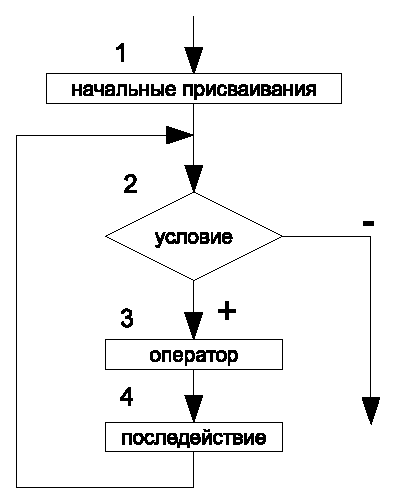
\includegraphics[width=0.3\textwidth]{img/ris_3_25}
\caption{Алгоритм работы цикла с параметром}
\label{ch03:refDrawing24}
\end{center}
\end{figure}

В дальнейшем, чтобы избежать создания слишком громоздких алгоритмов, в блок-схемах цикл \Sys{for} будем
изображать, так как показано на рис.~\ref{ch03:refDrawing25}.

В случае если тело цикла состоит более чем из одного оператора, необходимо использовать составной оператор:
\begin{lstlisting}
for `\Sys{(начальные\_присваивания; условие; последействие)}`
{
  `\Sys{оператор\_1;}`
  `\Sys{…}`
  `\Sys{оператор\_n;}`
}
\end{lstlisting}
Применение цикла \Sys{for} рассмотрим на примере печати таблицы значений функции  $y=e^{\sin (x)}\cos (x)$
на отрезке  $[0;\pi]$  с шагом 0.1:
\begin{figure}[htb]
\begin{center}
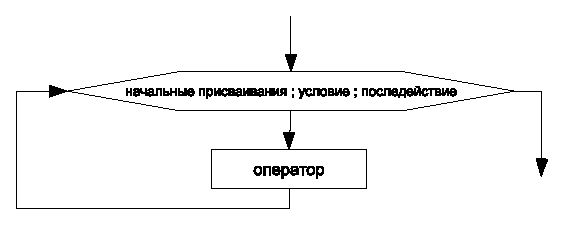
\includegraphics[width=0.5\textwidth]{img/ris_3_26}
\caption{Блок-схема цикла с параметром}
\label{ch03:refDrawing25}
\end{center}
\end{figure}

\begin{lstlisting}
#include <stdio.h>
#include <math.h>
#define PI 3.14159
using namespace std;
int main()
{
float x, y;
//`Параметру цикла присваивается начальное значение, если оно не превышает конечное значение,`
//`то выполняются операторы тела цикла и значение параметра изменяется, в противном случае`
//`цикл заканчивается.`
for (x=0;x<=PI;x+=0.1)
{
  y=exp(sin(x))*cos(x);
  printf("\t x=%5.2f \t y=%5.4f \n",x,y);
}
return 0;
}
\end{lstlisting}

Программный код выдаст результат, представленный на стр.~\pageref{ch03:out0}.% \ref{ch03:refDrawing22}.

\subsection[Операторы передачи управления]{Операторы передачи управления}
Операторы передачи управления принудительно изменяют порядок выполнения команд. В \Sys{С++} таких операторов четыре:
\Sys{goto}, \Sys{break}, \Sys{continue} и \Sys{return}.

Оператор \Sys{goto} \Sys{метка}, где \Sys{метка} обычный идентификатор, применяют
для безусловного перехода, он передаёт управление оператору с меткой: 
\Sys{метка: оператор};\footnote{Обычно применение оператора \Sys{goto} приводит к усложнению
программы и затрудняет отладку. Он нарушает принцип структурного программирования, согласно которому все блоки,
составляющие программу, должны иметь только один вход и один выход. В большинстве алгоритмов применения этого оператора
можно избежать}.

Оператор \Sys{break} осуществляет немедленный выход из циклов \Sys{while},
\Sys{do}…\Sys{while} и \Sys{for}, а так же из оператора выбора
\Sys{switch}. Управление передаётся оператору, находящемуся непосредственно за циклом или оператором
выбора. 

Оператор \Sys{continue} начинает новую итерацию цикла, даже если предыдущая не была завершена. 

Оператор \Sys{return} \Sys{выражение} завершает выполнение функции и передаёт управление в
точку её вызова. Если функция возвращает значение типа \Sys{void}, то выражение в записи оператора
отсутствует. В противном случае выражение должно иметь скалярный тип.

\section[Решение задач с использованием циклов]{Решение задач с использованием циклов}
Рассмотрим использование циклических операторов на конкретных примерах.

\prg{Написать программу решения квадратного уравнения
$ax^2+bx+c=0$. Предусмотреть проверку ввода данных.}{ch03:prg10}

Решение квадратного уравнения было подробно рассмотрено в задаче~\ref{ch03:prg4}. Однако алгоритм, изображённый 
на рис.~\ref{ch03:refDrawing14}, не будет работать, если пользователь введёт нулевое значение в переменную $a$ (при
попытке вычислить корни уравнения произойдёт деление на ноль). Чтобы избежать подобной ошибки нужно в программе
предусмотреть проверку входных данных, например, так как показано на рис.~\ref{ch03:refDrawing26}. 
Вводится значение переменной
$a$, если оно равно нулю, то ввод повторяется, иначе следует алгоритм вычисления корней квадратного
уравнения. Здесь применяется \emph{цикл с постусловием}, так как значение переменной необходимо ввести, а
затем проверить его на равенство нулю.

\begin{figure}[htb]
\begin{center}
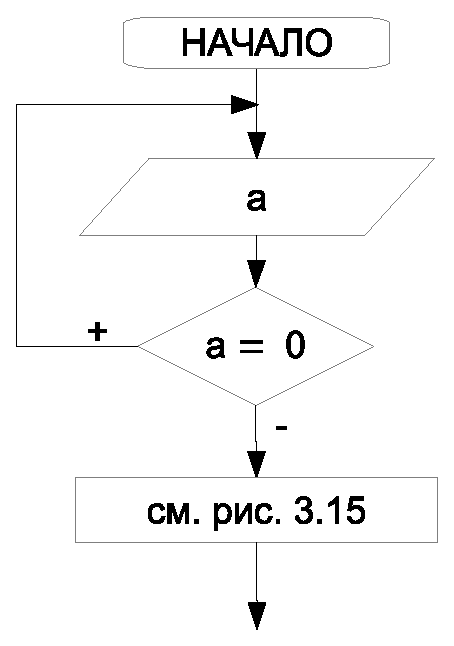
\includegraphics[width=0.3\textwidth]{img/ris_3_27}
\caption{Блок-схема проверки ввода данных}
\label{ch03:refDrawing26}
\end{center}
\end{figure}

Программа решения задачи:
\begin{lstlisting}
#include <iostream>
#include <math.h>
using namespace std;
int main()
{
float a,b,c,d,x1,x2;
//`Проверка ввода значения коэффициента` a.
do  //`Выполнять тело цикла пока а равно нулю`
{
  cout<<"a=";cin>>a;
}
while (a==0);
cout<<"b=";cin>>b;
cout<<"c=";cin>>c;
d=b*b-4*a*c;
if (d<0) cout<<"`Нет вещественных корней`";
else
{
x1=(-b+sqrt(d))/2/a;
x2=(-b-sqrt(d))/(2*a);
cout<<"X1="<<x1<<"\t X2="<<x2<<"\n";
}
return 0;
}
\end{lstlisting}

\prg{Найти наибольший общий делитель (НОД) натуральных чисел $A$
и $B$.}{ch03:prg11}

\emph{Входные данные}: $A$ и $B$.

\emph{Выходные данные}: $A$ --- НОД.

Для решения поставленной задачи воспользуемся алгоритмом Евклида: будем уменьшать каждый раз большее из чисел на
величину меньшего до тех пор, пока оба значения не станут равными, так, как показано в таблице~\ref{ch03:refTable1}. 


%%%%%%% Согласовать с авторами %%%%%%%%%
%{\tabcolsep=0.3em\noindent\small
%\begin{longtable}{|c|c|c|c|c|}
%\caption{Поиск НОД для чисел $A=25$ и $B=15$.} \label{ch03:refTable1}\\
%\hline
%\Emph{Исходные данные} & \Emph{Первый шаг} & \Emph{Второй шаг} & \Emph{Третий шаг} & \Emph{НОД(А,В)=5}\\
%\hline \hline
%\endfirsthead
%\multicolumn{5}{c}%
%{{\tablename\ \thetable{} --- продолжение}} \\
%\hline
%\Emph{Исходные данные} & \Emph{Первый шаг} & \Emph{Второй шаг} & \Emph{Третий шаг} & \Emph{НОД(А,В)=5}\\
%\hline \hline
%\endhead
%$A=25$ &$A=10$ &$A=10$ &$A=5$ &\\\hline
%$B=15$ &$B=15$ &$B=5$ &$B=5$ &\\\hline
%\end{longtable}
%}
%%%%%%%%%%%%%%%%%%%%%%%%%%%%%%%%
%{\tabcolsep=0.3em\noindent\small
\begin{longtable}{|l|c|c|}
\caption{Поиск НОД для чисел $A=25$ и $B=15$.} \label{ch03:refTable1}\\
\hline
\Emph{Шаг}&\Emph{A}&\Emph{B}\\
\hline\hline
\endfirsthead
\multicolumn{3}{c}%
{{\tablename\ \thetable{} --- продолжение}} \\
\hline
\Emph{Шаг}&\Emph{A}&\Emph{B}\\
\hline\hline
\endhead
Исходные данные&25&15\\\hline
Шаг 1&10&15\\\hline
Шаг 2&10&5\\\hline
Шаг 3, НОД&5&5\\\hline
\end{longtable}
%}
%%%%%%%%
%\begin{table}
%\begin{center}
%\caption{Поиск НОД для чисел $A=25$ и $B=15$.} \label{ch03:refTable1}
%\begin{tabular}{|l|c|c|}
%\hline
%\Emph{Шаг}&\Emph{A}&\Emph{B}\\
%\hline\hline
%Исходные данные&25&15\\\hline
%Шаг 1&10&15\\\hline
%Шаг 2&10&5\\\hline
%Шаг 3, НОД&5&5\\\hline
%\end{tabular}
%\end{center}
%\end{table}
%%%%%%%%%%%%

В блок–схеме, представленной на рис.~\ref{ch03:refDrawing27}, для решения поставленной задачи используется
\emph{цикл с предусловием}, то есть тело цикла повторяется до тех пор, пока $A$ не равно
$B$. Следовательно, при создании программы воспользуемся циклом \Sys{while}:

\begin{figure}[htb]
\begin{center}
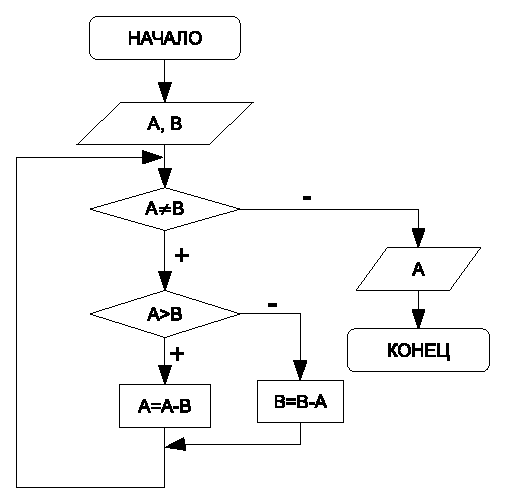
\includegraphics[width=0.5\textwidth]{img/ris_3_28}
\caption{Поиск наибольшего общего делителя двух чисел.}
\label{ch03:refDrawing27}
\end{center}
\end{figure}

\begin{lstlisting}
#include <iostream>
using namespace std;
int main()
{
  unsigned int a,b;
  cout<<"A="; cin>>a;
  cout<<"B="; cin>>b;
  //`Если числа не равны, выполнять тело цикла`
  while (a!=b)
  //`Если число` A `больше, чем` B, `то уменьшить его значение на` B,
    if (a>b) a=a-b;
  //`иначе уменьшить значение числа` B `на` A
    else b=b-a;
  cout<<"`НОД`="<<a<<"\n";
return 0;
}
\end{lstlisting}

Результат работы программы не изменится, если для её решения воспользоваться циклом с постусловием
\Sys{do…while}:

\begin{lstlisting}
#include <iostream>
using namespace std;
int main()
{
  unsigned int a,b;
  cout<<"A="; cin>>a;
  cout<<"B="; cin>>b;
  do
    if (a>b) a=a-b; else b=b-a;
  while (a!=b);
  cout<<"`НОД`="<<a<<"\n";
  return 0;
}
\end{lstlisting}

\prg{Вычислить факториал числа $N$ ( ${N}!=1\cdot 2\cdot 3\cdot \ldots \cdot N$).}{ch03:prg12}

\emph{Входные данные}: $N$ --- целое число, факториал которого необходимо вычислить.

\emph{Выходные данные}: \Sys{factorial} --- целое число, значение факториала числа $N$,
произведение чисел от 1 до $N$.

Промежуточные переменные: $i$ --- параметр цикла, целочисленная переменная, последовательно принимающая
значения 2, 3, 4 и так далее до $N$.

Блок-схема приведена на рис.~\ref{ch03:refDrawing28}.
\begin{figure}[htb]
\begin{center}
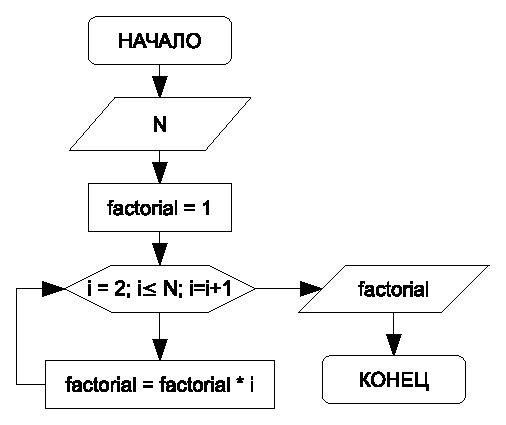
\includegraphics[width=0.5\textwidth]{img/ris_3_29}
\caption{Алгоритм вычисления факториала.}
\label{ch03:refDrawing28}
\end{center}
\end{figure}


Итак, вводится число $N$. Переменной \Sys{factorial}, предназначенной для хранения
значения произведения последовательности чисел, присваивается начальное значение, равное единице. Затем организуется
цикл, параметром которого выступает переменная $i$. Если значение параметра цикла не превышает
$N$, то выполняется оператор тела цикла, в котором из участка памяти с именем
\Sys{factorial} считывается предыдущее значение произведения, умножается на текущее значение параметра
цикла, а результат снова помещается в участок памяти с именем \Sys{factorial}. Когда параметр
$i$ превысит $N$, цикл заканчивается, и на экран выводится значение переменой
\Sys{factorial}, которая была вычислена в теле цикла.

Обратите внимание, как в программе записан \emph{оператор цикла}. Здесь операторы ввода и операторы
присваивания стартовых значений записаны как \Sys{начальные присваивания} цикла \Sys{for}, а
оператор накапливания произведения и оператор модификации параметра цикла представляют собой
\Sys{последействие}:
\begin{lstlisting}
#include <iostream>
using namespace std;
int main()
{
unsigned long long int factorial;1
unsigned int N, i;
for (cout<<"N=",cin>>N,factorial=1,i=2;i<=N;factorial*=i,i++);
cout<<"`факториал`="<<factorial<<"\n";
return 0;
}
\end{lstlisting}

\prg{Вычислить сумму натуральных чётных чисел, не превышающих~$N$.}{ch03:prg13}

\emph{Входные данные}: $N$ --- целое число.

\emph{Выходные данные}: $S$ --- сумма чётных чисел.

Промежуточные переменные: $i$ --- параметр цикла, принимает значения  2, 4, 6, 8 и так далее, также имеет
целочисленное значение.

При сложении нескольких чисел необходимо накапливать результат в определённом участке памяти (S), каждый раз считывая из
этого участка (S) предыдущее значение суммы (S) и прибавляя к нему слагаемое $i$. Для выполнения первого оператора
накапливания суммы из участка памяти необходимо взять такое число, которое не влияло бы на результат сложения. Перед
началом цикла переменной, предназначенной для накапливания сумы, необходимо присвоить значение нуль. Блок-схема решения
этой задачи представлена на рис.~\ref{ch03:refDrawing29}.

\begin{figure}[htb]
\begin{center}
\includegraphics[width=0.3\textwidth]{img/ris_3_30}
\caption{Алгоритм вычисления суммы чётных натуральных чисел.}
\label{ch03:refDrawing29}
\end{center}
\end{figure}

Решим задачу двумя способами: с применением циклов \Sys{while} и \Sys{for}:

\begin{lstlisting}
//`Решение задачи с помощью цикла` while
#include <iostream>
using namespace std;
int main()
{
  unsigned int N,i,S;
  cout<<"N="; cin>>N;
  S=0;
  i=2;
  while (i<=N)
  {
    S=S+i;
    i=i+2;
  }
  cout<<"S="<<S<<"\n";
  return 0;
}
//----------------------------------
//`Решение задачи с помощью цикла` for
#include <iostream>
using namespace std;
int main()
{
  unsigned int N,i,S;
  for (cout<<"N=",cin>>N,S=0,i=2;i<=N;S+=i,i+=2);
    cout<<"S="<<S<<"\n";
  return 0;
}
\end{lstlisting}

\prg{Дано натуральное число $N$. Определить
$K$ --- количество делителей этого числа, меньших самого числа (Например, для $N$=12
делители 1, 2, 3, 4, 6. Количество $K$=5).}{ch03:prg14}

\emph{Входные данные}: $N$ --- целое число.

\emph{Выходные данные}: целое число $K$ --- количество делителей~$N$.

Промежуточные переменные: $i$ --- параметр цикла, возможные делители числа~$N$.

В блок-схеме, изображённой на рис.~\ref{ch03:refDrawing30}, реализован следующий алгоритм: в переменную $K$,
предназначенную для подсчёта количества делителей заданного числа, помещается значение, которое не влияло бы на
результат, т.е. нуль. Далее организовывается цикл, в котором изменяющийся параметр $i$ выполняет роль
возможных делителей числа $N$. Если заданное число $N$ делится нацело на параметр цикла $i$, это
означает, что $i$ является делителем $N$, и значение переменной $K$
следует увеличить на единицу. Цикл необходимо повторить $\frac{N}{2}$ раз.

\begin{figure}[htb]
\begin{center}
\includegraphics[width=0.8\textwidth]{img/ris_3_31}
\caption{Алгоритм определения делителей натурального числа.}
\label{ch03:refDrawing30}
\end{center}
\end{figure}

Текст программы на \Sys{С++}:
\begin{lstlisting}
#include <iostream>
using namespace std;
int main()
{
  unsigned int N,i,K;
  cout<<"N="; cin>>N;
  for (K=0,i=1;i<=N/2;i++) if (N%i==0) K++;
  cout<<"K="<<K<<"\n";
  return 0;
}
\end{lstlisting}

\prg{Дано натуральное число $N$.
Определить, является ли оно простым. Натуральное число $N$ называется простым, если оно делится без
остатка только на единицу и на само себя. Число 13 --- простое, так как делится только на 1 и 13, а число 12 таковым не
является, так как делится на 1, 2, 3, 4, 6 и 12.}{ch03:prg15}

\emph{Входные данные}: $N$ --- целое число.

\emph{Выходные данные}: сообщение.

Промежуточные переменные: $i$ --- параметр цикла, возможные делители числа~$N$.

Необходимо проверить, есть ли делители числа $N$ в диапазоне от $2$ до $N/2$ (рис.~\ref{ch03:refDrawing31}). Если
делителей нет, $N$ --- простое число, иначе оно таковым не является. Обратите внимание на то, что в
алгоритме предусмотрено два выхода из цикла. Первый --- естественный, при исчерпании всех значений параметра, 
а второй --- досрочный. Нет смысла продолжать цикл, если будет найден хотя бы один  делитель из указанной области изменения
параметра.

\begin{figure}[htb]
\begin{center}
\includegraphics[width=0.5\textwidth]{img/ris_3_32}
\caption{Алгоритм определения простого числа.}
\label{ch03:refDrawing31}
\end{center}
\end{figure}

При составлении программы на языке \Sys{С++} досрочный выход из цикла удобно выполнять при помощи оператора
\Sys{break}:
\begin{lstlisting}
#include <iostream>
using namespace std;
int main()
{
unsigned int N,i;
bool Pr;
cout<<"N="; cin>>N;
Pr=true;  //`Предположим, что число простое`
for (i=2;i<=N/2;i++)
  if (N%i==0) //`Если найдётся хотя бы один делитель, то`
  {
    Pr=false; //`число простым не является и`
    break; //`досрочный выход из цикла`
  }
  if (Pr) //`Проверка значения логического параметра и вывод на печать`
          //`соответствующего сообщения`
    cout<<N<<" - `\Sys{простое число}`\n";
  else
    cout<<N<<" - `\Sys{не является простым}`\n";
return 0;
}
\end{lstlisting}

\prg{Дано натуральное число $N$. Определить количество цифр в числе.}{ch03:prg16}

\emph{Входные данные}: $N$ --- целое число.

\emph{Выходные данные}: $kol$ --- количество цифр в числе.

\emph{Промежуточные данные}: $M$ --- переменная для временного хранения значения
$N$\footnote{При решении задачи (см. алгоритм на рис.~\ref{ch03:refDrawing32}) исходное число изменятся,
поэтому, чтобы его, не потерять, копируем исходное число $N$ в переменную $M$, и делить будем уже $M$.}.

Для того, чтобы подсчитать количество цифр в числе, необходимо определить, сколько раз заданное число можно разделить на
десять нацело. Например, пусть $N=12345$, тогда количество цифр $kol = 5$. Результаты
вычислений сведены в таблицу \ref{ch03:refTable2}.

\begin{longtable}{|c|c|}
\caption{Определение количества цифр числа} \label{ch03:refTable2}\\
\hline
\Emph{kol} & \Emph{N}\\
\hline \hline
\endfirsthead
\multicolumn{2}{c}%
{{\tablename\ \thetable{} --- продолжение}} \\
\hline
\Emph{kol} & \Emph{N}\\
\hline \hline
\endhead
1 & 12345\\\hline
2 & 12345 / 10 = 1234\\\hline
3 & 1234 / 10 = 123\\\hline
4 & 123 / 10 = 12\\\hline
5 & 12 / 10 = 1\\\hline
 & 1 / 10 = 0\\\hline
\end{longtable}

Алгоритм определения количества цифр в числе представлен на рис.~\ref{ch03:refDrawing32}.

\begin{figure}[htb]
\begin{center}
\includegraphics[width=0.5\textwidth]{img/ris_3_33}
\caption{Алгоритм определения количества цифр в числе.}
\label{ch03:refDrawing32}
\end{center}
\end{figure}

\begin{lstlisting}
#include <iostream>
using namespace std;
int main()
{
	unsigned long int N, M;
	unsigned int kol;
	cout<<"N="; cin>>N;
	for (M=N, kol=1; M/10>0; kol++,M/=10);
	cout<<"kol="<<kol<<endl;
return 0;
}
\end{lstlisting}

\prg{Дано натуральное число $N$. Определить,
содержит ли это число нули и в каких разрядах они расположены (например, число 11011110111 содержит ноль в третьем и
восьмом разрядах, а число 120405 ---  в первом и третьем).}{ch03:prg17}

\emph{Входные данные}: $N$ --- целое число. 

\emph{Выходные данные}: $pos$ --- позиция цифры в числе. 

\emph{Промежуточные данные}: $i$ --- параметр цикла, $M$ --- переменная для
временного хранения значения $N$.

В связи с тем, что разряды в числе выделяются начиная с последнего, для определения номера разряда в числе,
необходимо знать количество цифр в числе\footnote{Алгоритм нахождения количества цифр в числе был рассмотрен в
предыдущей задаче.}. Таким образом, на первом этапе решения задачи необходимо определить $kol$ ---
количество цифр в числе. Затем нужно выделять из числа цифры, если очередная цифра равна нулю, вывести на экран номер
разряда, который занимает эта цифра. Процесс определения текущей цифры числа
$N=120405$ представлен в таблице~\ref{ch03:refTable3}.

\begin{longtable}{|c|l|l|c|}
\caption{Определение текущей цифры числа} \label{ch03:refTable3}\\
\hline
\Emph{i} & \Emph{Число М} & \Emph{Цифра} & \Emph{Номер позиции}\\
\hline \hline
\endfirsthead
\multicolumn{4}{c}%
{{\tablename\ \thetable{} --- продолжение}} \\
\hline
\Emph{i} & \Emph{Число М} & \Emph{Цифра} & \Emph{Номер позиции}\\
\hline \hline
\endhead
1 & 120405 & 120405 \% 10 = 5 &0\\\hline
2 & 12040/10 = 1204 & 12040 \% 10 = 0 & \Emph{1}\\\hline
3 & 1204/10 = 120 & 1204 \% 10 = 4 & 2\\\hline
4 & 120/10 = 12 & 120 \% 10 = 0 & \Emph{3}\\\hline
5 & 12/10 = 1 & 12 \% 10 = 2 & 4\\\hline
6 & 1/10 = 0 & 1 \% 10 = 1 & 5\\\hline
\end{longtable}

Программный код к задаче~\ref{ch03:prg17}.
\begin{lstlisting}
#include <iostream>
using namespace std;
int main()
{
  unsigned long int N,M; int kol, i;
  cout<<"N="; cin>>N;
  for (kol=1,M=N;M/10>0; kol++,M/=10);
    for (M=N,i=0;i<kol;M/=10,i++)
      if (M%10==0) cout<<"`\Sys{Позиция}` = "<<i<<endl;
  return 0;
}
\end{lstlisting}

\prg{Дано натуральное число $N$. Получить
новое число, записав цифры числа $N$ в обратном порядке. Например, 17852 --- 25871.}{ch03:prg18}

\emph{Входные данные}: $N$ --- целое число.

\emph{Выходные данные}: $S$ --- целое число, полученное из цифр числа $N$, записанных в обратном порядке.

\emph{Промежуточные данные}: $i$ --- параметр цикла, $M$ --- переменная для
временного хранения значения $N$, $kol$ --- количество разрядов в заданном числе, 
$R=10^{kol}$ --- старший разряд заданного числа.

Рассмотрим пример. Пусть $N=17852$, тогда 
$S=2\cdot 10^4+5\cdot 10^3+8\cdot 10^2+7\cdot 10^1+1\cdot 10^0=25871$.

Значит, для решения поставленной задачи, нужно знать количество
разрядов в заданном числе $kol$ и его старший разряд $R=10^{kol}$.
Новое число $S$ формируют как сумму произведений
последней цифры заданного числа на старший разряд $S+=M\%10*R$. Цикл выполняют
$kol$ раз, при каждой итерации уменьшая само число и старший разряд в десять раз.
\begin{lstlisting}
#include <iostream>
using namespace std;
int main()
{unsigned long int N,M,R,S; int kol, i;
cout<<"N="; cin>>N;
for (R=1,kol=1,M=N;M/10>0; kol++,R*=10,M/=10);
  for(S=0,M=N,i=1;i<=kol;S+=M%10*R,M/=10,R/=10,i++);
    cout<<"S="<<S<<endl;
return 0;
}
\end{lstlisting}

\prg{Проверить, является ли заданное число $N$ палиндромом\protect\footnotemark . 
Например, числа 404, 1221 --- палиндромы.}{ch03:prg19}%
\footnotetext{
Палиндром --- это число, слово или фраза одинаково читающееся в обоих направлениях, или, другими
словами, любой симметричный относительно своей середины набор символов.
}

\emph{Входные данные}: $N$ --- целое число.

\emph{Выходные данные}: \Sys{сообщение}. 

\emph{Промежуточные данные}: $i$ --- параметр цикла, $M$ --- переменная для
временного хранения значения $N$, $kol$ --- количество разрядов в заданном числе,
$R=10^{kol}$ --- старший разряд заданного числа, $S$ --- целое число, полученное 
из цифр числа $N$, записанных в обратном порядке.

Можно предложить следующий алгоритм решения задачи. Записать цифры заданного числа $N$ в обратном
порядке (задача~\ref{ch03:prg18}), получится новое число $S$.
Сравнить полученное число $S$ с исходным $N$. Если числа равны,
то заданное число является палиндромом.

Текст программы на языке \Sys{С++}:
\begin{lstlisting}
#include <iostream>
using namespace std;
int main()
{unsigned long int N,M,R,S; 
int kol, i;
cout<<"N="; cin>>N;
for (R=1,kol=1,M=N;M/10>0; kol++,R*=10,M/=10);
  for(S=0,M=N,i=1;i<=kol;S+=M%10*R,M/=10,R/=10,i++);
    if (N==S) cout<<"`\Sys{Число - палинром}`"<<endl;
    else cout<<"`\Sys{Число не является палиндромом}`"<<endl;
return 0;
}
\end{lstlisting}


\prg{Поступает последовательность из $N$ вещественных чисел.
Определить наибольший элемент последовательности.}{ch03:prg20}

\emph{Входные данные}: $N$ --- целое число; $X$ --- вещественное число,
определяет текущий элемент последовательности.

\emph{Выходные данные}: $Max$ --- вещественное число, элемент последовательности с
наибольшим значением.

\emph{Промежуточные переменные}: $i$ --- параметр цикла, номер вводимого элемента
последовательности.

Алгоритм поиска наибольшего элемента в последовательности следующий (рис.~\ref{ch03:refDrawing33}). 
Вводится $N$ --- количество элементов последовательности и $X$ --- первый элемент последовательности. 
В памяти компьютера отводится ячейка, например с
именем $Max$, в которой будет храниться наибольший элемент последовательности --- максимум. Далее
предполагаем, что первый элемент последовательности наибольший и записываем его в $Max$. Затем
вводим второй элемент последовательности и сравниваем его с предполагаемым максимумом. Если окажется, что второй
элемент больше, его записывают в ячейку $Max$. В противном случае никаких действий не предпринимаем.
Потом переходим к вводу следующего элемента последовательности ($X$), и алгоритм повторяется с начала. В результате в
ячейке $Max$ сохранится элемент последовательности с наибольшим значением\footnote{Для поиска
наименьшего элемента последовательности (минимума), предполагают, что первый элемент --- наименьший, записывают его в
ячейку $min$, а затем среди элементов последовательности ищут число, значение которого будет меньше чем предполагаемый
минимум.}.

\begin{figure}[htb]
\begin{center}
\includegraphics[width=0.5\textwidth]{img/ris_3_34}
\caption{Алгоритм поиска наибольшего числа в последовательности.}
\label{ch03:refDrawing33}
\end{center}
\end{figure}

Текст программы на \Sys{С++}:
\begin{lstlisting}
#include <iostream>
using namespace std;
int main()
{
  unsigned int i,N;
  float X,Max;
  cout<<"N="; cin>>N;
  cout<<"X="; cin>>X; //`Ввод первого элемента последовательности`
  //`Параметр цикла принимает стартовое значение` i=2, `т.к. первый элемент`
  //`уже введён предположим, что он максимальный, т.е.` Max=X.
  for (i=2, Max=X; i<=N;i++)
  {
    cout<<"X="; cin>>X; //`Ввод следующих элементов последовательности.`
  //`Если найдётся элемент, превышающий максимум, записать его в ячейку` Max, 
  //`теперь он предполагаемый максимум.`
  if (X>Max) Max=X;
  }
  //`Вывод наибольшего элемента последовательности.`
  cout<<"Max="<<Max<<"\n";
  return 0;
}
\end{lstlisting}

\prg{Вводится последовательность целых чисел, 0 --- конец последовательности. Найти
наименьшее число среди положительных, если таких значений несколько\protect\footnote{Предположим вводится последовательность
чисел 11, -3, 5, 12, -7, 5, 8,-9, 7, -6, 10, 5, 0. Наименьшим положительным числом является 5. Таких минимумов в
последовательности 3.}, определить, сколько их.}{ch03:prg21}

%\footnote{
%Предположим вводится последовательность
%чисел 11, -3, 5, 12, -7, 5, 8,-9, 7, -6, 10, 5,0. Наименьшим положительным числом является 5. Таких минимумов в
%последовательности 3.
%}

Блок-схема решения задачи приведена на рис. \ref{ch03:refDrawing34}.
\begin{figure}[htb]
\begin{center}
\includegraphics[width=0.8\textwidth]{img/ris_3_35}
\caption{Алгоритм поиска минимального положительного числа в последовательности.}
\label{ch03:refDrawing34}
\end{center}
\end{figure}

Далее приведён текст подпрограммы с подробными комментариями\footnote{Алгоритм поиска максимального (минимального)
элементов последовательности подробно описан в задаче~\ref{ch03:prg20}}.

\begin{lstlisting}
#include <iostream>
using namespace std;
int main()
{
  float N,Min; int K;
  //`Предположим, что в последовательности нет положительных чисел`, K=0.
  //`Вводим число и если оно не равно нулю`
  for (cout<<"N=",cin>>N,K=0;N!=0;cout<<"N=",cin>>N)
    //`проверяем является ли оно положительным.`
    if (N>0)
      //`если K=0, поступил 1-й положительный элемент, предположим, что он минимальный.`
      if (K==0) {K=1;Min=N;}
        //`если элемент не первый, сравниваем его с предполагаемым минимумом,`
        //`если элемент меньше, записываем его в` Min `и сбрасываем счётчик`
      else if (N<Min) {Min=N;K=1;}
           //`если элемент равен минимуму, увеличиваем значение счётчика.`
           else if (N==Min) K++; //`Конец цикла`
  //`Если значение счётчика не равно нулю, печатаем значение`
  //`минимального элемента и количество таких элементов.`
  if (K!=0) cout<<"Min="<<Min<<"\n"<<"K="<<K<<"\n";
  //`в противном случае выдаём сообщаем.`
  else cout<<"`\Sys{В последовательности нет положительных элементов}` \n";
  return 0;
}
\end{lstlisting}


\prg{Определить, сколько раз последовательность из
$N$ произвольных чисел меняет знак.}{ch03:prg22}

Чтобы решить задачу, нужно попарно перемножать элементы последовательности. Если результат произведения пары чисел ---
отрицательное число, значит, эти числа имеют разные знаки. 

Пусть в переменной $B$ хранится текущий элемент последовательности, в $A$ --- предыдущий. Введём первое 
число $A$ (до цикла) и
второе $B$ (в цикле). Если их произведение отрицательно, то увеличиваем количество смен знака на 1 (\Sys{k++}). После чего
сохраняем значение $B$ в переменную $A$ и повторяем цикл (рис.~\ref{ch03:refDrawing35}).

\begin{figure}[htb]
\begin{center}
\includegraphics[width=0.6\textwidth]{img/ris_3_36}
\caption{Алгоритм решения задачи~\ref{ch03:prg22}.}
\label{ch03:refDrawing35}
\end{center}
\end{figure}

Предлагаем читателю самостоятельно разобраться с текстом программы на \Sys{С++}: 
\begin{lstlisting}
#include <iostream>
using namespace std;
int main()
{
  float A,B; int i,K,N;
  cout<<"N=";cin>>N;
  for (K=0,cout<<"A=",cin>>A,i=2;i<=N;i++)
  {
    cout<<"B=";cin>>B;
    if (A*B<0) K++;
    A=B;
  }
  cout<<"K="<<K<<"\n";
  return 0;
}
\end{lstlisting}


\prg{Поступает последовательность из $N$ вещественных чисел. Определить количество
простых чисел в последовательности.}{ch03:prg23}

Блок-схема алгоритма изображена на рис.~\ref{ch03:refDrawing36}. Обратите внимание, что для решения задачи было организовано два
цикла. Первый цикл обеспечивает ввод элементов последовательности. Второй цикл находится внутри первого и определяет,
является ли поступившее число простым (задача~\ref{ch03:prg15}).

\begin{figure}[htb]
\begin{center}
\includegraphics[width=0.5\textwidth]{img/ris_3_37}
\caption{Алгоритм поиска простых чисел в последовательности.}
\label{ch03:refDrawing36}
\end{center}
\end{figure}

\begin{lstlisting}
#include <iostream>
using namespace std;
int main()
{
  unsigned long int X; 
  unsigned int N; 
  int i,k,j;
  bool Pr;
  for (k=0,cout<<"N=", cin>>N, i=1;i<=N;i++)
  {
    for (cout<<"X=", cin>>X,Pr=true,j=2;j<=X/2;j++)
      if (X%j==0) 
      {
        Pr=false;
        break;
      }
      if (Pr) k++;
  }
  if (k==0) cout<<"`\Sys{Простых чисел нет}` \n";
  else  cout<<"`\Sys{Количество простых чисел}` k="<<k<<"\n";
return 0;
}
\end{lstlisting}

\prg{Дано $K$ наборов ненулевых целых чисел. Каждый набор
содержит не менее двух элементов, признаком его завершения является число 0. Найти количество наборов, элементы которых
возрастают.}{ch03:prg24}

Блок-схема алгоритма решения задачи показана на рис.~\ref{ch03:refDrawing37}. Нетрудно заметить, что алгоритм реализован с
помощью двух циклических процессов. Внутренний цикл проверяет является ли последовательность возрастающей, а внешний
повторяет алгоритм для новой последовательности.

\begin{figure}[htb]
\begin{center}
\includegraphics[width=0.6\textwidth]{img/ris_3_38}
\caption{Алгоритм решения задачи~\ref{ch03:prg24}.}
\label{ch03:refDrawing37}
\end{center}
\end{figure}

Программный код решения задачи~\ref{ch03:prg24}:
\begin{lstlisting}
#include <iostream>
using namespace std;
int main()
{
  unsigned int K, i,kol, A, B; bool pr;
  for (cout<<"K=", cin>>K, kol=0,i=1;i<=K;i++)
  {
    for (pr=true,cout<<"A=",cin>>A;A!=0; A=B)
    {
      cout<<"B="; cin>>B;
      if (B!=0 && A>=B) pr=false;
    }
    if (pr) kol++;
  }
  cout << "kol=" << kol<<endl;
  return 0;
}
\end{lstlisting}


\section[Задачи для самостоятельного решения]{Задачи для самостоятельного решения}
\subsection[Разветвляющийся процесс. Вычисление значения функции.]{Разветвляющийся процесс. Вычисление значения
функции.}
Разработать программу на языке \Sys{С++}. Дано вещественное число $a$. Для функции
$y=f(x)$, график которой приведён ниже, вычислить
$f(a)$. Варианты заданий представлены на рис.~\ref{ch03:refDrawing38}--\ref{ch03:refDrawing62}.

%%%%%% рис 39, 40 и 41 в ряд 
\floatsetup[widefloat]{margins=hangleft}
\begin{figure}[h]%
\begin{floatrow}[3]
\ffigbox[\FBwidth]
{\caption{Задание~1}%
\label{ch03:refDrawing38}}
{\includegraphics[width=0.32\textwidth,keepaspectratio]{img/ris_3_39}}
\ffigbox[\FBwidth]
{\caption{Задание~2}%
\label{ch03:refDrawing39}}
{\includegraphics[width=0.32\textwidth,keepaspectratio]{img/ris_3_40}}
\ffigbox[\FBwidth]
{\caption{Задание~3}%
\label{ch03:refDrawing40}}
{\includegraphics[width=0.32\textwidth,keepaspectratio]{img/ris_3_41}}
\end{floatrow}
\end{figure}%
%%%% end 39, 40, 41

%%%%%% рис 42, 43 и 44 в ряд 
\floatsetup[widefloat]{margins=hangleft}
\begin{figure}[h]%
\begin{floatrow}[3]
\ffigbox[\FBwidth]
{\caption{Задание~4}%
\label{ch03:refDrawing41}}
{\includegraphics[width=0.32\textwidth,keepaspectratio]{img/ris_3_42}}
\ffigbox[\FBwidth]
{\caption{Задание~5}%
\label{ch03:refDrawing42}}
{\includegraphics[width=0.32\textwidth,keepaspectratio]{img/ris_3_43}}
\ffigbox[\FBwidth]
{\caption{Задание~6}%
\label{ch03:refDrawing43}}
{\includegraphics[width=0.32\textwidth,keepaspectratio]{img/ris_3_44}}
\end{floatrow}
\end{figure}%
%%%% end 42, 43, 44

%%%%%% рис 45, 46 и 47 в ряд 
\floatsetup[widefloat]{margins=hangleft}
\begin{figure}%
\begin{floatrow}[3]
\ffigbox[\FBwidth]
{\caption{Задание~7}%
\label{ch03:refDrawing44}}
{\includegraphics[width=0.32\textwidth,keepaspectratio]{img/ris_3_45}}
\ffigbox[\FBwidth]
{\caption{Задание~8}%
\label{ch03:refDrawing45}}
{\includegraphics[width=0.32\textwidth,keepaspectratio]{img/ris_3_46}}
\ffigbox[\FBwidth]
{\caption{Задание~9}%
\label{ch03:refDrawing46}}
{\includegraphics[width=0.32\textwidth,keepaspectratio]{img/ris_3_47}}
\end{floatrow}
\end{figure}%
%%%% end 45, 46, 47

%%%%%% рис 48, 49 и 50 в ряд 
\floatsetup[widefloat]{margins=hangleft}
\begin{figure}%
\begin{floatrow}[3]
\ffigbox[\FBwidth]
{\caption{Задание~10}%
\label{ch03:refDrawing47}}
{\includegraphics[width=0.32\textwidth,keepaspectratio]{img/ris_3_48}}
\ffigbox[\FBwidth]
{\caption{Задание~11}%
\label{ch03:refDrawing48}}
{\includegraphics[width=0.32\textwidth,keepaspectratio]{img/ris_3_49}}
\ffigbox[\FBwidth]
{\caption{Задание~12}%
\label{ch03:refDrawing49}}
{\includegraphics[width=0.32\textwidth,keepaspectratio]{img/ris_3_50}}
\end{floatrow}
\end{figure}%
%%%% end 48, 49, 50

%%%%%% рис 51, 52 и 53 в ряд 
\floatsetup[widefloat]{margins=hangleft}
\begin{figure}%
\begin{floatrow}[3]
\ffigbox[\FBwidth]
{\caption{Задание~13}%
\label{ch03:refDrawing50}}
{\includegraphics[width=0.32\textwidth,keepaspectratio]{img/ris_3_51}}
\ffigbox[\FBwidth]
{\caption{Задание~14}%
\label{ch03:refDrawing51}}
{\includegraphics[width=0.32\textwidth,keepaspectratio]{img/ris_3_52}}
\ffigbox[\FBwidth]
{\caption{Задание~15}%
\label{ch03:refDrawing52}}
{\includegraphics[width=0.32\textwidth,keepaspectratio]{img/ris_3_53}}
\end{floatrow}
\end{figure}%
%%%% end 51, 52, 53

%%%%%% рис 54, 55 и 56 в ряд 
\floatsetup[widefloat]{margins=hangleft}
\begin{figure}%
\begin{floatrow}[3]
\ffigbox[\FBwidth]
{\caption{Задание~16}%
\label{ch03:refDrawing53}}
{\includegraphics[width=0.32\textwidth,keepaspectratio]{img/ris_3_54}}
\ffigbox[\FBwidth]
{\caption{Задание~17}%
\label{ch03:refDrawing54}}
{\includegraphics[width=0.32\textwidth,keepaspectratio]{img/ris_3_55}}
\ffigbox[\FBwidth]
{\caption{Задание~18}%
\label{ch03:refDrawing55}}
{\includegraphics[width=0.32\textwidth,keepaspectratio]{img/ris_3_56}}
\end{floatrow}
\end{figure}%
%%%% end 54, 55, 56

%%%%%% рис 57, 58 и 59 в ряд 
\floatsetup[widefloat]{margins=hangleft}
\begin{figure}%
\begin{floatrow}[3]
\ffigbox[\FBwidth]
{\caption{Задание~19}%
\label{ch03:refDrawing56}}
{\includegraphics[width=0.32\textwidth,keepaspectratio]{img/ris_3_57}}
\ffigbox[\FBwidth]
{\caption{Задание~20}%
\label{ch03:refDrawing57}}
{\includegraphics[width=0.32\textwidth,keepaspectratio]{img/ris_3_58}}
\ffigbox[\FBwidth]
{\caption{Задание~21}%
\label{ch03:refDrawing58}}
{\includegraphics[width=0.32\textwidth,keepaspectratio]{img/ris_3_59}}
\end{floatrow}
\end{figure}%
%%%% end 57, 58, 59

%%%% рис 60 и 61 бок о бок
\begin{figure}[h]
\begin{floatrow}
\floatbox{figure}[.35\textwidth][\FBheight][t]
{\caption{Задание~22}
\label{ch03:refDrawing59}}
{\includegraphics[width=0.32\textwidth,keepaspectratio]{img/ris_3_60}}%\hspace*{0.05\textwidth}
%
\floatbox{figure}[.35\textwidth][\FBheight][b]
{\caption{Задание~23}
\label{ch03:refDrawing60}}
{\includegraphics[width=0.32\textwidth]{img/ris_3_61}}
\end{floatrow}
\end{figure}

%%%% рис 62 и 63 бок о бок
\begin{figure}[h]
\begin{floatrow}
\floatbox{figure}[.35\textwidth][\FBheight][t]
{\caption{Задание~24}
\label{ch03:refDrawing61}}
{\includegraphics[width=0.32\textwidth,keepaspectratio]{img/ris_3_62}}%\hspace*{0.05\textwidth}
%
\floatbox{figure}[.35\textwidth][\FBheight][b]
{\caption{Задание~25}
\label{ch03:refDrawing62}}
{\includegraphics[width=0.32\textwidth]{img/ris_3_63}}
\end{floatrow}
\end{figure}

\subsection[Разветвляющийся процесс. Попадание точки в область на плоскости]{Разветвляющийся процесс. Попадание точки в
область на плоскости}
Разработать программу на языке \Sys{С++}. Даны вещественные числа $x$ и $y$. Определить,
принадлежит ли точка с координатами ($x$; $y$) заштрихованной области.
Варианты заданий представлены на рис.~\ref{ch03:refDrawing63}--\ref{ch03:refDrawing87}.


%%%%%% рис 64, 65 и 66 в ряд 
\floatsetup[widefloat]{margins=hangleft}
\begin{figure}[h]%
\begin{floatrow}[3]
\ffigbox[\FBwidth]
{\caption{Задание~1}%
\label{ch03:refDrawing63}}
{\includegraphics[width=0.32\textwidth,keepaspectratio]{img/ris_3_64}}
\ffigbox[\FBwidth]
{\caption{Задание~2}%
\label{ch03:refDrawing64}}
{\includegraphics[width=0.32\textwidth,keepaspectratio]{img/ris_3_65}}
\ffigbox[\FBwidth]
{\caption{Задание~3}%
\label{ch03:refDrawing65}}
{\includegraphics[width=0.32\textwidth,keepaspectratio]{img/ris_3_66}}
\end{floatrow}
\end{figure}%
%%%% end 64, 65, 66

%%%%%% рис 67, 68 и 69 в ряд 
\floatsetup[widefloat]{margins=hangleft}
\begin{figure}[h]%
\begin{floatrow}[3]
\ffigbox[\FBwidth]
{\caption{Задание~4}%
\label{ch03:refDrawing66}}
{\includegraphics[width=0.32\textwidth,keepaspectratio]{img/ris_3_67}}
\ffigbox[\FBwidth]
{\caption{Задание~5}%
\label{ch03:refDrawing67}}
{\includegraphics[width=0.32\textwidth,keepaspectratio]{img/ris_3_68}}
\ffigbox[\FBwidth]
{\caption{Задание~6}%
\label{ch03:refDrawing68}}
{\includegraphics[width=0.32\textwidth,keepaspectratio]{img/ris_3_69}}
\end{floatrow}
\end{figure}%
%%%% end 67, 68, 69

%%%%%% рис 70, 71 и 72 в ряд 
\floatsetup[widefloat]{margins=hangleft}
\begin{figure}[h]%
\begin{floatrow}[3]
\ffigbox[\FBwidth]
{\caption{Задание~7}%
\label{ch03:refDrawing69}}
{\includegraphics[width=0.32\textwidth,keepaspectratio]{img/ris_3_70}}
\ffigbox[\FBwidth]
{\caption{Задание~8}%
\label{ch03:refDrawing70}}
{\includegraphics[width=0.32\textwidth,keepaspectratio]{img/ris_3_71}}
\ffigbox[\FBwidth]
{\caption{Задание~9}%
\label{ch03:refDrawing71}}
{\includegraphics[width=0.32\textwidth,keepaspectratio]{img/ris_3_72}}
\end{floatrow}
\end{figure}%
%%%% end 70, 71, 72

%%%%%% рис 73, 74 и 75 в ряд 
\floatsetup[widefloat]{margins=hangleft}
\begin{figure}[h]%
\begin{floatrow}[3]
\ffigbox[\FBwidth]
{\caption{Задание~10}%
\label{ch03:refDrawing72}}
{\includegraphics[width=0.32\textwidth,keepaspectratio]{img/ris_3_73}}
\ffigbox[\FBwidth]
{\caption{Задание~11}%
\label{ch03:refDrawing73}}
{\includegraphics[width=0.32\textwidth,keepaspectratio]{img/ris_3_74}}
\ffigbox[\FBwidth]
{\caption{Задание~12}%
\label{ch03:refDrawing74}}
{\includegraphics[width=0.32\textwidth,keepaspectratio]{img/ris_3_75}}
\end{floatrow}
\end{figure}%
%%%% end 73, 74, 75

%%%%%% рис 76, 77 и 78 в ряд 
\floatsetup[widefloat]{margins=hangleft}
\begin{figure}[h]%
\begin{floatrow}[3]
\ffigbox[\FBwidth]
{\caption{Задание~13}%
\label{ch03:refDrawing75}}
{\includegraphics[width=0.32\textwidth,keepaspectratio]{img/ris_3_76}}
\ffigbox[\FBwidth]
{\caption{Задание~14}%
\label{ch03:refDrawing76}}
{\includegraphics[width=0.32\textwidth,keepaspectratio]{img/ris_3_77}}
\ffigbox[\FBwidth]
{\caption{Задание~15}%
\label{ch03:refDrawing77}}
{\includegraphics[width=0.32\textwidth,keepaspectratio]{img/ris_3_78}}
\end{floatrow}
\end{figure}%
%%%% end 76, 77, 78

%%%%%% рис 79, 80 и 81 в ряд 
\floatsetup[widefloat]{margins=hangleft}
\begin{figure}[h]%
\begin{floatrow}[3]
\ffigbox[\FBwidth]
{\caption{Задание~16}%
\label{ch03:refDrawing78}}
{\includegraphics[width=0.30\textwidth,keepaspectratio]{img/ris_3_79}}
\ffigbox[\FBwidth]
{\caption{Задание~17}%
\label{ch03:refDrawing79}}
{\includegraphics[width=0.30\textwidth,keepaspectratio]{img/ris_3_80}}
\ffigbox[\FBwidth]
{\caption{Задание~18}%
\label{ch03:refDrawing80}}
{\includegraphics[width=0.30\textwidth,keepaspectratio]{img/ris_3_81}}
\end{floatrow}
\end{figure}%
%%%% end 79, 80, 81

%%%%%% рис 82, 83 и 84 в ряд 
\floatsetup[widefloat]{margins=hangleft}
\begin{figure}[h]%
\begin{floatrow}[3]
\ffigbox[\FBwidth]
{\caption{Задание~19}%
\label{ch03:refDrawing81}}
{\includegraphics[width=0.30\textwidth,keepaspectratio]{img/ris_3_82}}
\ffigbox[\FBwidth]
{\caption{Задание~20}%
\label{ch03:refDrawing82}}
{\includegraphics[width=0.26\textwidth,keepaspectratio]{img/ris_3_83}}
\ffigbox[\FBwidth]
{\caption{Задание~21}%
\label{ch03:refDrawing83}}
{\includegraphics[width=0.30\textwidth,keepaspectratio]{img/ris_3_84}}
\end{floatrow}
\end{figure}%
%%%% end 82, 83, 84

%%%% рис 85 и 86 бок о бок
\begin{figure}[h]
\begin{floatrow}
\floatbox{figure}[.35\textwidth][\FBheight][t]
{\caption{Задание~22}
\label{ch03:refDrawing84}}
{\includegraphics[width=0.32\textwidth,keepaspectratio]{img/ris_3_85}}%\hspace*{0.05\textwidth}
%
\floatbox{figure}[.35\textwidth][\FBheight][b]
{\caption{Задание~23}
\label{ch03:refDrawing85}}
{\includegraphics[width=0.28\textwidth]{img/ris_3_86}}
\end{floatrow}
\end{figure}

%%%% рис 87 и 88 бок о бок
\begin{figure}[h]
\begin{floatrow}
\floatbox{figure}[.35\textwidth][\FBheight][t]
{\caption{Задание~24}
\label{ch03:refDrawing86}}
{\includegraphics[width=0.28\textwidth,keepaspectratio]{img/ris_3_87}}%\hspace*{0.05\textwidth}
%
\floatbox{figure}[.35\textwidth][\FBheight][b]
{\caption{Задание~25}
\label{ch03:refDrawing87}}
{\includegraphics[width=0.28\textwidth]{img/ris_3_88}}
\end{floatrow}
\end{figure}


\subsection[Разветвляющийся процесс. Пересечение линий и решение уравнений.]{Разветвляющийся процесс. Пересечение
линий и решение уравнений.}
Разработать программу на языке \Sys{С++} для следующих заданий:

\begin{enumerate}
\item Задан круг с центром в точке $O(x_0, y_0)$, радиусом $R_0$ и точка $A(x_1,y_1)$. 
Определить, находится ли точка внутри круга.
\item Задана окружность с центром в точке $O(x_0,y_0)$ и радиусом $R_0$. Определить, пересекается ли
заданная окружность с осью абсцисс, если пересекается --- найти точки пересечения.
\item Задана окружность с центром в точке $O(x_0,y_0)$ и радиусом $R_0$. Определить, пересекается ли
заданная окружность с осью ординат, если пересекается --- найти точки пересечения.
\item Задана окружность с центром в точке $O(0,0)$ и радиусом $R_0$ и
прямая $y=ax+b$. Определить, пересекаются ли прямая и
окружность. Если пересекаются, найти точки пересечения.
\item Заданы окружности. Первая с центром в точке $O(x_1,y_1)$ и радиусом
$R_1$, вторая с центром в точке $O(x_2,y_2)$ и радиусом
$R_2$. Определить, пересекаются окружности, касаются или не пересекаются.
\item Заданы три точки
$A(x_1,y_1)$, $B(x_2,y_2)$,$C(x_3,y_3)$. Определить, какая
из точек наиболее удалена от начала координат.
\item Заданы три точки $A(x_1,y_1)$, $B(x_2,y_2)$, $C(x_3,y_3)$. Определить, какая
из точек $B$ или $C$ наименее удалена от точки $A$.
\item Определить, пересекаются ли линии $y=ax+b$ и
$y=kx+m$. Если пересекаются, найти точку пересечения.
\item Определить, пересекает ли линия $y=ax+b$ ось абсцисс. Если пересекает, найти точку пересечения.
\item Определить, пересекаются ли линии
$y=ax^3+bx^2+cx+d$ и $y=kx+m$. Если пересекаются, найти точки пересечения.
\item Определить, пересекаются ли линии
$y=ax^3+bx^2+cx+d$
и
$y=kx^3+mx^2+nx+p$.
Если пересекаются, найти точки пересечения.
\item Определить, пересекаются ли линии
$y=ax^3+bx^2+cx+d$
и
$y=ax^3+mx^2+nx+p$.
Если пересекаются, найти точки пересечения.
\item Определить, пересекаются ли линии
$y=ax^3+bx^2+cx+d$
и $y=mx^2+nx+p$. Если
пересекаются, найти точку пересечения.
\item Определить, пересекает ли линия
$y=ax^3+bx^2+cx+d$
ось абсцисс. Если пересекает, найти точку пересечения.
\item Определить, пересекаются ли параболы
$y=ax^2+bx+c$ и $y=dx^2+mx+n$. Если
пересекаются, то найти точки пересечения.
\item Определить, пересекаются ли линии
$y=bx^2+cx+d$ и
$y=kx+m$. Если пересекаются, найти точки пересечения
\item Найти точки пересечения линии
$y=ax^2+bx+c$ с осью
абсцисс. Если линии не пересекаются выдать соответствующее сообщение.
\item Определить, пересекаются ли линии
$y=ax^4+bx^3+cx^2+dx+f$
и
$y=bx^3+mx^2+dx+p$.
Если пересекаются, найти точки пересечения.
\item Определить, пересекаются ли линии
$y=ax^4+bx^2+kx+c$
и
$y=mx^2+kx+p$.
Если пересекаются, найти точки пересечения.
\item Определить, пересекает ли линия
$y=ax^4+bx^2+c$
ось абсцисс. Если пересекает, найти точки пересечения.
\item Найти комплексные корни уравнения
$y=ax^4+bx^2+c$.
Если в уравнении нет комплексных корней, вывести соответствующее сообщение.
\item Найти комплексные корни уравнения
$y=ax^3+bx^2+cx+d$. Если в
уравнении нет комплексных корней, вывести соответствующее сообщение.
\item Найти комплексные корни уравнения $y=ax^2+bx+c$. Если в
уравнении нет комплексных корней, вывести соответствующее сообщение.
\item Заданы точки $A(x_1,y_1,z_1)$ и $B(x_2,y_2,z_2)$. Определить, какая из точек наименее удалена от начала координат.
\item Даны координаты точки, не лежащей на координатных осях $OX$ и $OY$. Определить номер координатной четверти, в которой
находится данная точка.
\end{enumerate}

\subsection[Циклический процесс. Вычисление значений функции]{Циклический процесс. Вычисление значений функции}

Разработать программу на языке \Sys{С++}. Для решения задачи использовать операторы \Sys{for},
\Sys{while}, \Sys{do}. Варианты заданий:

\begin{enumerate}
\item Вывести на экран таблицу значений функции синус в диапазоне от  $-2\cdot \pi $ до  $2\cdot \pi $  с шагом~
$\frac{\pi}{8}$.
\item Вывести на экран таблицу квадратов первых десяти целых положительных чисел.
\item Вывести на экран таблицу значений функции косинус в диапазоне от  $-2\cdot \pi $  до  $2\cdot \pi $  с шагом~
$\frac{\pi}{8}$.
\item Вывести на экран таблицу кубов первых десяти целых положительных чисел.
\item Вывести на экран таблицу значений квадратов синусов в диапазоне от  $-\pi$  до  $\pi$  с шагом~$\frac{\pi}{12}$.
\item Вывести на экран таблицу значений квадратов косинусов в диапазоне от 0 до $2\cdot \pi$ с шагом~$\frac{\pi}{10}$.
\item Вывести на экран таблицу квадратов первых десяти целых чётных положительных чисел.
\item Вывести на экран таблицу квадратов первых десяти целых нечётных положительных чисел.
\item Вывести на экран таблицу значений удвоенных синусов в диапазоне от $-a$ до $a$ с шагом $h$. Значения $a$ и
 $h$  вводятся с клавиатуры.
\item Вывести на экран таблицу значений удвоенных косинусов в диапазоне от  $a$  до  $b$  с шагом  $h$. Значения  $a$,
 $b$  и  $h$  вводятся с клавиатуры.
\item Вывести на экран таблицу кубов первых десяти целых нечётных положительных чисел.
\item Вывести на экран таблицу кубов первых десяти целых чётных положительных чисел.
\item Вывести на экран таблицу значений функции  $y=e^{2x}$ в диапазоне от  $-a$  до  $a$  с шагом  $h$. Значения  $a$ 
и  $h$  вводятся с клавиатуры.
\item Вывести на экран таблицу значений функции  $y=5\cdot e^{-3x}$  в диапазоне от  $a$  до  $b$  с шагом~$h$.
Значения  $a$,  $b$  и  $h$  вводятся с клавиатуры.
\item Вывести на экран таблицу квадратов первых десяти целых отрицательных чисел.
\item Вывести на экран таблицу кубов первых десяти целых отрицательных чисел.
\item Вывести на экран таблицу квадратных корней первых десяти целых положительных чисел.
\item Вывести на экран таблицу кубических корней первых десяти целых положительных чисел.
\item Вывести на экран таблицу значений функции  $y=2\cdot x^2+3\cdot x-1$  в диапазоне от  $-a$  до  $a$  с шагом~
$h$. Значения  $a$  и  $h$  вводятся с клавиатуры.
\item Вывести на экран таблицу значений функции  $y=5.4\cdot x^{3}-2.8\cdot x^{2}-x+1.6$  в диапазоне от  $a$  до  $b$ 
с шагом  $h$. Значения  $a$,  $b$  и  $h$  вводятся с клавиатуры.
\item Вывести на экран таблицу квадратных корней первых десяти целых положительных чётных чисел.
\item Вывести на экран таблицу квадратных корней первых десяти целых положительных нечётных чисел.
\item Вывести на экран таблицу значений функции  $y=-1.8\cdot x^3-e^2x+\frac{1}{6}$  в диапазоне от  $-3$ до  $4$  с
шагом~$\frac{1}{2}$.
\item Вывести на экран таблицу значений функции  $y=-1.3\cdot x^2-\frac{e^x}{4}$  в диапазоне от  $-2$  до  $2$  с
шагом~$\frac{1}{4}$.
\item Вывести на экран таблицу степеней двойки в диапазоне от  0  до  10  с шагом~1.
\end{enumerate}

\subsection[Циклический процесс. Последовательности натуральных чисел]{Циклический процесс. Последовательности
натуральных чисел}
Разработать программу на языке \Sys{С++} для следующих заданий:

\begin{enumerate}
\item Дано целое положительное число $N$. Вычислить сумму натуральных нечётных чисел не превышающих
это число.
\item Дано целое положительное число $N$. Вычислить произведение натуральных чётных чисел не
превышающих это число.
\item Дано целое положительное число $N$. Вычислить количество натуральных чисел кратных трём и не
превышающих число~$N$.
\item Задано целое положительное число $n$. Определить значение выражения:
 $\displaystyle P=\frac{n!}{\sum\limits_{i=1}^{n}i}.$
\item Вычислить количество натуральных двузначных чётных чисел не делящихся на~10.
\item Задано целое положительное число $n$. Определить значение выражения:
$\displaystyle P=\frac{\sum\limits_{i=1}^ni^2}{n!}.$
\item Вычислить сумму натуральных удвоенных чисел не превышающих~25.
\item Задано целое положительное число $n$. Определить значение выражения:
$P=\frac{\sum\limits_{i=3}^{n}i-2}{(n+1)!}.$
\item Дано целое положительное число $N$. Вычислить сумму квадратов натуральных чётных чисел не
превышающих это число.
\item Дано целое положительное число $N$. Вычислить количество натуральных чисел кратных пяти и не
превышающих число $N$.
\item Определить значение выражения:
 $P=\frac{\sum\limits_{i=0}^{5}3^{i}}{5!}.$
\item Дано целое положительное число $N$. Вычислить сумму удвоенных натуральных нечётных чисел не
превышающих это число.
\item Задано целое положительное число $n$. Определить значение выражения:
 $P=\sum\limits_{i=2}^{n}i^{2}-i.$
\item Найти сумму нечётных степеней двойки. Значение степени изменяется от 1 до~9.
\item Задано целое положительное число $n$. Определить значение выражения:
 $P=\frac{1}{3}\cdot {\sum\limits_{i=1}^{n}2\cdot i^{2}-i+1}.$
\item Дано целое положительное число $N$. Вычислить произведение натуральных чисел кратных трём и не
превышающих число~$N$.
\item Задано целое положительное число $n$. Определить значение выражения:
 $P=\sum\limits_{i=3}^{n+2}2\cdot i-4.$
\item Вычислить сумму натуральных трёхзначных чисел кратных пяти и не делящихся на десять.
\item Определить значение выражения:
 $P=\sum\limits_{i=0}^{10}2^{i}.$
\item Вычислить количество натуральных двузначных нечётных чисел не делящихся на~5.
\item Задано целое положительное число $n$. Определить значение выражения:
 $P=\frac{\sum\limits_{i=0}^{n-1}i+1}{(2n)!}.$
\item Задано целое положительное число $n$. Определить значение выражения:
 $P=\frac{\sum\limits_{i=5}^{15}i}{(2\cdot n+1)!}.$
\item Найти произведение чётных степеней двойки. Значение степени изменяется от 0 до~8.
\item Вычислить произведение натуральных чисел не превышающих~15.
\item Вычислить произведение натуральных двузначных чисел кратных трём и не делящихся на~10.
\end{enumerate}

\subsection[Циклический процесс. Последовательности произвольных чисел]{Циклический процесс. Последовательности
произвольных чисел}
Разработать программу на языке \Sys{С++} для следующих заданий:

\begin{enumerate}
\item Вводится последовательность ненулевых чисел, 0 --- конец последовательности. Определить сумму положительных
элементов последовательности.
\item Вычислить сумму отрицательных элементов последовательности из $N$ произвольных чисел.
\item Вводится последовательность ненулевых чисел, 0 --- конец последовательности. Определить, сколько раз
последовательность поменяет знак.
\item В последовательности из $N$ произвольных чисел подсчитать количество нулей.
\item Вводится последовательность ненулевых чисел, 0 --- конец последовательности. Определить наибольшее число в
последовательности.
\item Вводится последовательность из $N$ произвольных чисел найти наименьшее число в
последовательности.
\item Вводится последовательность ненулевых чисел, 0 --- конец последовательности. Определить среднее значение элементов
последовательности.
\item Вводится последовательность из $N$ произвольных чисел, найти среднее значение положительных
элементов последовательности.
\item Вводится последовательность ненулевых чисел, 0 --- конец последовательности. Подсчитать процент положительных и
отрицательных чисел.
\item Вводится последовательность из $N$ произвольных чисел. Определить процент положительных,
отрицательных и нулевых элементов. 
\item Вводится последовательность из $N$ произвольных чисел. Вычислить разность между наименьшим и
наибольшим значениями последовательности.
\item Вводится последовательность из $N$ положительных целых чисел. Найти наименьшее число среди
чётных элементов последовательности.
\item Вводится последовательность из $N$ целых чисел. Определить, является ли эта
последовательность знакочередующейся.
\item Определить, является ли последовательность из $N$ произвольных чисел строго возрастающей (каждый
следующий элемент больше предыдущего).
\item Вводится последовательность произвольных чисел, 0 --- конец последовательности. Определить, является ли эта
последовательность строго убывающей (каждый следующий элемент меньше предыдущего).
\item Вводится последовательность ненулевых целых чисел, 0 --- конец последовательности. Определить среднее значение
чётных элементов последовательности.
\item Вводится последовательность из $N$ произвольных чисел, найти среднее значение отрицательных
элементов последовательности.
\item В последовательности из $N$ целых чисел подсчитать количество чётных и нечётных чисел.
\item Вводится последовательность целых чисел, 0 --- конец последовательности. Определить процент чётных и нечётных чисел
в последовательности.
\item Вводится последовательность из $N$ целых чисел. Определить, содержит ли последовательность хотя
бы два соседних одинаковых числа.
\item Вводится последовательность целых чисел, 0 --- конец последовательности. Определить наибольшее число среди нечётных
элементов последовательности.
\item Вводится последовательность произвольных чисел, 0 --- конец последовательности. Определить сумму и количество чисел
в последовательности.
\item Вводится последовательность из $N$ произвольных чисел. Найти сумму положительных и сумму
отрицательных элементов последовательности.
\item Вводится последовательность произвольных чисел, 0 --- конец последовательности. Определить отношение минимального и
максимального элементов друг к другу.
\item Вводится последовательность из $N$ целых чисел. Определить количество одинаковых рядом стоящих
чисел.
\end{enumerate}

\subsection[Циклический процесс. Работа с цифрами в числе]{Циклический процесс. Работа с цифрами в числе}
Разработать программу на языке \Sys{С++} для следующих заданий:

\begin{enumerate}
\item Определить, является ли целое положительное число \emph{совершённым}. Совершённое число равно сумме
всех своих делителей, не превосходящих это число. Например, 6=1+2+3 или 28=1+2+4+7+14.
\item Проверить, является ли пара целых положительных чисел \emph{дружественными}. Два различных натуральных
числа являются дружественными, если сумма всех делителей первого числа (кроме самого числа) равна второму числу.
Например, 220 и 284, 1184 и 1210, 2620 и 2924, 5020 и 5564.
\item Определить, является ли целое положительное число \emph{недостаточным}. Недостаточное число всегда
больше суммы всех своих делителей за исключением самого числа.
\item Вводится целое положительное число. Определить количество чётных и нечётных цифр в числе.
\item Вводится целое положительное число. Найти число, которое равно сумме кубов цифр исходного числа.
\item Вводится целое положительное число. Определить, совпадает ли сумма цифр, 
расположенных до середины числа, с суммой цифр расположенных после. Например, задано число из восьми 
цифр 12112021. Здесь, сумма первых четырёх цифр, равна сумме следующих четырёх цифр $1+2+1+1=2+0+2+1=5$. 
Или, задано число из семи цифр 3456444, тогда $3+4+5=4+4+4=12$. Здесь цифра 6 не учитывается.
\item Вводится целое положительное число. Найти суммы чётных и нечётных цифр заданного числа.
\item Задано целое положительное число. Определить количество его чётных и нечётных делителей.
\item Проверить, являются ли два целых положительных числа \emph{взаимно простыми}. Два различных
натуральных числа являются взаимно простыми, если их наибольший общий делитель равен единице.
\item Определить, является ли целое положительное число \emph{составным}. Составное число имеет более двух
делителей, то есть не является \emph{простым}.
\item Вводится целое положительное число. Найти наименьшую цифру числа.
\item Задано целое положительное число. Определить, является ли оно \emph{числом Армстронга}. Число
Армстронга --- натуральное число, которое равно сумме своих цифр, возведённых в степень, равную количеству его цифр.
Например, десятичное число 153 --- число Армстронга, потому что:  $1^3+3^3+5^3=1+27+125=153$.
\item Вводится целое положительное число. Найти произведение всех ненулевых цифр числа.
\item Вводится целое положительное число. Найти наибольшую цифру числа.
\item Вводится целое положительное число. Определить позицию наибольшей цифры в числе.
\item Вводится целое положительное число. Найти число, которое равно сумме удвоенных цифр исходного числа.
\item Вводится целое положительное число. Найти число, которое равно сумме квадратов цифр исходного числа.
\item Задано целое положительное число. Определить сумму его делителей.
\item Вводится целое положительное число. Определить позицию наименьшей цифры в числе.
\item Проверить, что два целых положительных числа не являются \emph{взаимно простыми}. Различные
натуральные числа не являются взаимно простыми, если их наибольший общий делитель отличен от единицы.
\item Убедиться, что заданное целое положительное число не является \emph{палиндромом}. Числа-палиндромы
симметричны относительно своей середины, например, 12021 или 454.
\item Убедиться, что заданное целое положительное число не является \emph{совершённым}. Совершённое число
равно сумме всех своих делителей, не превосходящих это число. Например, 6=1+2+3 или 28=1+2+4+7+14.
\item Проверить, что два целых положительных числа не являются \emph{дружественными}. Два различных
натуральных числа являются дружественными, если сумма всех делителей первого числа (кроме самого числа) равна второму
числу. Например, 220 и 284, 1184 и 1210, 2620 и 2924, 5020 и 5564.
\item Вводится целое положительное число. Найти число, которое равно сумме утроенных цифр исходного числа.
\item Вводятся два целых положительных числа. Найти сумму их цифр. 
\end{enumerate}

\subsection[Вложенные циклы]{Вложенные циклы}
Разработать программу на языке \Sys{С++} для следующих заданий:

\begin{enumerate}
\item Дано натуральное число $P$. Вывести все простые числа не
превосходящие $P$.
\item Дано натуральное число $P$. Вывести все совершённые числа не превосходящие
$P$.
\item Вводится последовательность положительных целых чисел, 0 --- конец последовательности. Определить количество
совершённых чисел в последовательности.
\item Вводится последовательность положительных целых чисел, 0 --- конец последовательности. Определить количество простых
чисел в последовательности.
\item Вводится последовательность из $N$ положительных целых чисел. Для каждого элемента
последовательности вычислить факториал.
\item Вводится последовательность из $N$ положительных целых чисел. Вывести на экран все числа ---
палиндромы. Если таких чисел нет, выдать соответствующее сообщение.
\item Вводится последовательность из $N$ положительных целых чисел. Определить разрядность каждого
числа.
\item Вводится последовательность из $N$ положительных целых чисел. Вывести на экран количество
делителей каждого числа.
\item Вводится последовательность положительных целых чисел, 0 --- конец последовательности. Определить сумму цифр каждого
элемента последовательности.
\item Дано $K$ наборов ненулевых целых чисел. Признаком завершения каждого набора является число 0. Для каждого набора
вывести количество его элементов. Вычислить общее количество элементов.
\item Дано $K$ наборов ненулевых целых чисел. Признаком завершения каждого набора является число 0. Для каждого набора
вычислить среднее арифметическое его элементов.
\item Даны $K$ наборов целых чисел по $N$ элементов в каждом наборе. Для каждого набора найти наибольшее значение его
элементов.
\item Даны $K$ наборов целых чисел по $N$ элементов в каждом наборе. Определить, есть ли среди наборов данных
знакочередующиеся последовательности.
\item Даны $K$ наборов целых чисел по $N$ элементов в каждом наборе. Определить, есть ли среди наборов данных строго
возрастающие последовательности.
\item Дано $K$ наборов ненулевых целых чисел. Признаком завершения каждого набора является число 0. Для каждого набора
найти наименьшее значение его элементов.
\item Даны $K$ наборов целых чисел по $N$ элементов в каждом наборе. Для каждого набора вычислить произведение ненулевых
элементов.
\item Даны $K$ наборов целых чисел по $N$ элементов в каждом наборе. Найти наибольшее число для всех наборов.
\item Дано $K$ наборов ненулевых целых чисел. Признаком завершения каждого набора является число 0. Вычислить среднее
арифметическое всех элементов во всех наборах.
\item Дано $K$ наборов ненулевых целых чисел. Признаком завершения каждого набора является число 0. Найти количество
возрастающих наборов.
\item Дано $K$ наборов ненулевых целых чисел. Признаком завершения каждого набора является число 0. Найти количество
убывающих наборов.
\item Дано $K$ наборов ненулевых целых чисел. Признаком завершения каждого набора является число 0. Найти количество
наборов не являющихся знакочередующимися.
\item Дано $K$ наборов ненулевых целых чисел. Признаком завершения каждого набора является число 0. Найти количество
наборов элементы которых не возрастают и не убывают.
\item Даны целые положительные числа $N$ и $M$ ($N<M$). Вывести все целые числа от $N$ до $M$ включительно; при этом
каждое число должно выводиться столько раз, каково его значение (например, число 5 выводится 5 раз).
\item Дано целое число $N>0$. Найти сумму 1! + 2! + 3! + … + $N$!
\item Даны целые числа $N$ и $M$ ($N<M$). Вывести все целые числа от $N$ до $M$ включительно; при этом число $N$ должно
выводиться 1 раз, число $N + 1$ должно выводиться 2 раза и т. д.
\end{enumerate}

\chapter[Использование функций при программировании на \Sys{C++}]{Использование функций при программировании на \Sys{C++}}\label{ch04}
В практике программирования часто складываются ситуации, когда одну и ту же группу операторов, реализующих определенную
цель, требуется повторить без изменений в нескольких местах программы. Для избавления от столь нерациональной траты
времени была предложена концепция подпрограммы.

\index{Подпрограмма}\emph{Подпрограмма} --- именованная, логически законченная группа операторов языка,
которую можно вызвать для выполнения любое количество раз из различных мест программы. В языке \Sys{C++} подпрограммы
реализованы в виде \index{Функция}\emph{функций}~\cite{KR}.

\section[Общие сведения о функциях]{Общие сведения о функциях. Локальные и
глобальные переменные}
\index{Функция}\emph{Функция} --- это поименованный набор описаний и операторов, выполняющих определенную
задачу. Функция может принимать параметры и возвращать значение. Информация, передаваемая в функцию для обработки,
называется \emph{параметром}, а результат вычисления функции ее \emph{значением}. Обращение к
функции называют \emph{вызовом}. Как известно (п.~\ref{ch02:8}) любая программа на \Sys{C++} состоит из одной или
нескольких функций. При запуске программы первой выполняется функция \Sys{main}. Если среди операторов
функции \Sys{main} встречается вызов функции, то управление передается операторам функции. Когда все
операторы функции будут выполнены, управление возвращается оператору, следующему за вызовом функции.

Перед вызовом функция должна быть обязательно описана. \index{Функция!описание}\emph{Описание функции}
состоит из заголовка и тела функции:
\begin{lstlisting}
`\Sys{тип имя\_функции(список\_переменных)}`
{
  `\Sys{тело\_функции}`
}
\end{lstlisting}
\index{Функция!заголовок}\emph{Заголовок функции} содержит:

\begin{itemize}
\item \Sys{тип}, возвращаемого функцией значения, он может быть любым; если функция не возвращает значения,
указывают тип \Sys{void};
\item \Sys{имя\_функции;}
\item \Sys{список\_переменных} --- перечень передаваемых в функцию величин (\emph{аргументов}),
которые отделяются друг от друга запятыми; для каждой переменной из списка указывается \Sys{тип} и
\Sys{имя}; если функция не имеет аргументов, то в скобках указывают либо тип \Sys{void}, либо
ничего.
\end{itemize}
\index{Функция!тело функции}\emph{Тело функции} представляет собой последовательность описаний и
операторов, заключенных в фигурные скобки.

В общем виде \emph{структура программы} на \Sys{C++} может иметь вид:
\begin{lstlisting}
`\Sys{директивы компилятора}`
`\Sys{тип имя\_1(список\_переменных)}`
{
  `\Sys{тело\_функции\_1;}`
}

`\Sys{тип имя\_2(список\_переменных)}`
{
  `\Sys{тело\_функции\_2;}`
}

`\Sys{...}`

`\Sys{тип имя\_n(список\_переменных)}`
{
  `\Sys{тело\_функции\_n;}`
}

int main(`\Sys{список\_переменных}`)
{
  //`Тело функции может содержать операторы вызова функций \Sys{имя\_1, имя\_2, ..., имя\_n}`
  `\Sys{тело\_основной\_функции;}`
}
\end{lstlisting}
Однако допустима и другая \emph{форма записи программного кода}:

\begin{lstlisting}
`\Sys{директивы компилятора}`
`\Sys{тип имя\_1(список\_переменных);}`
`\Sys{тип имя\_2(список\_переменных);}`
`\Sys{...}`
`\Sys{тип имя\_n(список\_переменных);}`
int main(`\Sys{список\_переменных}`)
{
  //`Тело функции может содержать операторы вызова функций \Sys{имя\_1, имя\_2, ..., имя\_n}`
  `\Sys{тело\_основной\_функции;}`
}
`\Sys{тип имя\_1(список\_переменных)}`
{
  `\Sys{тело\_функции\_1;}`
}

`\Sys{тип имя\_2(список\_переменных)}`
{
  `\Sys{тело\_функции\_2;}`
}

`\Sys{...}`

`\Sys{тип имя\_n(список\_переменных)}`
{
  `\Sys{тело\_функции\_n;}`
}
\end{lstlisting}

Здесь функции описаны после функции \Sys{main()}, однако до нее перечислены заголовки всех функций. Такого
рода опережающие заголовки называют \index{Функция!прототип}\emph{прототипами
функций}. Прототип указывает компилятору тип данных, возвращаемых функцией, тип переменных,
выступающих в роли аргументов и порядок их следования. Прототипы используются для проверки правильности вызова функций
в основной программе. Имена переменных, указанные в прототипе функции, компилятор игнорирует:
\begin{lstlisting}
//`Записи равносильны.`
int func(int a,int b);
int func(int ,int);
\end{lstlisting}

\index{Функция!вызов}\emph{Вызвать функцию} можно в любом месте программы. Для \emph{вызова
функции} необходимо указать ее \Sys{имя} и в круглых скобках, через запятую перечислить
\Sys{имена} или \Sys{значения аргументов}, если таковые имеются:

\begin{lstlisting}
`\Sys{имя\_функции(список\_переменных);}`
\end{lstlisting}

Рассмотрим пример. Создадим функцию \Sys{f()}, которая не имеет входных значений и не формирует результат.
При вызове этой функции на экран выводится строка символов \Sys{"Happy new year, "}.

\begin{lstlisting}
#include <iostream>
using namespace std;
void f()  //`Описание функции.`
{
  cout << "Happy new year, ";
}
int main()
{
  f();      //`Вызов функции.`
  cout <<"Students!" << endl;
  f();      //`Вызов функции.`
  cout <<"Teachers!" << endl;
  f();      //`Вызов функции.`
  cout <<"People!" << endl;
}
\end{lstlisting}

Результатом работы программы будут три строки:
\begin{verbatim}
Happy new year, Students!
Happy new year, Teachers!
Happy new year, People!
\end{verbatim}

Далее приведен пример программы, которая пять раз выводит на экран фразу \Sys{"Hello
World!"}. Операция вывода строки символов оформлена в виде функции \Sys{fun()}. Эта функция так же
не имеет входных значений и не формирует результат. Вызов функции осуществляется в цикле:
\begin{lstlisting}
#include <iostream>
using namespace std;
void fun()
{
  cout << "Hello World!" << endl;
}

int main()
{
  for(int i=1;i<=5;fun(),i++);
}
\end{lstlisting}

Если тип возвращаемого значения не \Sys{void}, то функция может входить в состав выражений.
\emph{Типы и порядок следования переменных в определении и при вызове функции должны совпадать}. Для того
чтобы \index{Функция!возврат результата}\emph{функция вернула} какое-либо значение, в ней должен быть
оператор: 

\Sys{return (выражение);}

Далее приведен пример программы, которая вычисляет значение выражения  
$\sin^2(\alpha)+\cos^2(\alpha)=1$ при заданном значении  $\alpha$. Здесь функция \Sys{radian} выполняет
перевод градусной меры угла в радианную\footnote{Чтобы найти радианную меру какого-нибудь угла по заданной градусной
мере, нужно помножить число градусов на  $\frac{\pi}{180}$, число минут на  $\frac{\pi}{180\cdot 60}$, число секунд
на и  $\frac{\pi}{180\cdot 60\cdot 60}$ найденные произведения сложить.}.
\begin{lstlisting}
#include <iostream>
#include <math.h>
#define PI 3.14159
using namespace std;
double radian(int deg, int min, int sec)
{
  return (deg*PI/180+min*PI/180/60+sec*PI/180/60/60);
}
int main()
{
  int DEG,MIN,SEC; double RAD;
  //`Ввод данных.`
  cout<<"Inpout:"<<endl;   //`Величина угла:`
  cout<<"DEG="; cin>>DEG;  //`градусы,`
  cout<<"MIN="; cin>>MIN;  //`минуты,`
  cout<<"SEC="; cin>>SEC;  //`секунды.`
  //`Величина угла в радианах.`
  RAD=radian(DEG,MIN,SEC); //`Вызов функции.`
  cout << "Value in radian A="<<RAD << endl;
  //`Вычисление значения выражения и его вывод.`
  cout << "sin(A)^2+cos(A)^2=";
  cout << pow(sin(RAD),2)+pow(cos(RAD),2) << endl;
  return 0;
}
\end{lstlisting}


Переменные, описанные внутри функции, а так же переменные из списка аргументов, являются
\index{Переменная!локальная}\emph{локальными}. Например, если программа содержит пять разных функций, в
каждой из которых описана переменная $N$, то для \Sys{C++} это пять различных переменных. Область действия локальной переменной
не выходит за рамки функции. Значения локальных переменных между вызовами одной и той же функции не сохраняются. 

Переменные, определенные до объявления всех функций и доступные всем функциям, называют
\index{Переменная!глобальная}\emph{глобальными}. В функции глобальную переменную можно отличить, если не
описана локальная переменная с теми же именем.

Глобальные переменные применяют для передачи данных между функциями, но это затрудняет отладку программы. Для обмена
данными между функциями используют параметры функций и значения, возвращаемые функциями.

\section[Передача параметров в функцию]{Передача параметров в функцию}
Обмен информацией между вызываемой и вызывающей функциями осуществляется с помощью \index{Функция!механизм передачи
параметров}\emph{механизма передачи параметров}. \Sys{Список\_переменных}, указанный в
заголовке функции называется \index{Функция!формальные параметры}\emph{формальными параметрами} или просто
\emph{параметрами} функции. \Sys{Список\_переменных} в операторе вызова функции --- это
\index{Функция!фактические параметры}\emph{фактические параметры} или \emph{аргументы}. 

\emph{Механизм передачи параметров обеспечивает замену формальных параметров фактическими параметрами}, и
позволяет выполнять функцию с различными данными. Между фактическими параметрами в операторе вызова функции и
формальными параметрами в заголовке функции устанавливается взаимно однозначное соответствие.
\emph{Количество, типы и порядок следования формальных и фактических параметров должны совпадать}.

\index{Передача параметров}\emph{Передача параметров} выполняется следующим образом. Вычисляются выражения,
стоящие на месте фактических параметров. В памяти выделяется место под формальные параметры в соответствии с их
типами. Затем формальным параметрам присваиваются значения фактических. Выполняется проверка типов и при необходимости
выполняется их преобразование. При несоответствии типов выдается диагностическое сообщение. 

Передача параметров в функцию может осуществляться \index{Передача параметров!по значению}\emph{по
значению} и \index{Передача параметров!по адресу}\emph{по адресу}. 

При передаче данных по значению функция работает с копиями фактических параметров, и доступа к исходным значениям
аргументов у нее нет. При передаче данных по адресу в функцию передается не переменная, а ее адрес, и, следовательно,
функция имеет доступ к ячейкам памяти, в которых хранятся значения аргументов. Таким образом, данные, переданные по
значению, функция изменить не может, в отличие от данных, переданных по адресу. 

Если требуется запретить изменение параметра внутри функции, используют модификатор \Sys{const}. Заголовок
функции в общем виде будет выглядеть так:
\begin{lstlisting}
`\Sys{тип имя\_функции}`(const `\Sys{тип\_переменной* имя\_переменной, …)}`
\end{lstlisting}

Например:
\begin{lstlisting}
#include <iostream>
using namespace std;
int f1(int i)  //`Данные передаются по значению`
{
  return(i++);
}
int f2(int* j) //`Данные передаются по адресу. При подстановке фактического параметра,` 
               //`для получения его значения, применяется операция разадресации *`.
{
  return((*j)++);
}
int f3(const int* k)  //`Изменение параметра не предусмотрено`.
{
  return(*k);
}
int main()
{
  int a;
  cout<<"a=";cin>>a;
  f1(a);
  cout<<"a="<<a<<"\n";
  f2(&a); //`Для передачи фактического параметра используется операция взятия адреса \&`.
  cout<<"a="<<a<<"\n";
  f3(&a);
  cout<<"a="<<a<<"\n";
  return 0;
}
\end{lstlisting}

Результат работы программы:
\begin{verbatim}
Введено значение переменной a.
a=5 
Значение переменной a после вызова функции f1 не изменилось.
a=5 
Значение переменной a после вызова функции f2 изменилось.
a=6 
Значение переменной a после вызова функции f3 не изменилось.
a=6 
\end{verbatim}

Удобно использовать передачу данных по адресу, если нужно чтобы функция изменяла значения переменных в вызывающей
программе.

Далее приведен пример программы, в которой исходя из радианной меры  некоторого угла вычисляется величина смежного с ним
угла. На экран выводятся значения углов в градусной мере. Функция \Sys{degree} выполняет перевод из
радианной меры в градусную\footnote{Чтобы найти градусную меру угла по заданной радианной нужно помножить число радиан
на  $\frac{180}{\pi }$ ; если из полученной дроби выделить целую часть, то получим градусы; если из числа полученного
умножением оставшейся дробной части 60 выделить целую часть получим минуты; секунды вычисляются аналогично из дробной
части минут.}. Эта функция ничего не возвращает. Ее аргументами являются \emph{значение} переменной
\Sys{rad}, определяющее величину угла в радианах и \emph{адреса} переменных
\Sys{deg}, \Sys{min}, \Sys{sec}, в которых будут храниться вычисленные
результаты --- градусная мера угла. 
\begin{lstlisting}
#include <iostream>
#include <math.h>
#define PI 3.14159
using namespace std;
void degree (double rad, int* deg, int* min, int* sec)
{
  *deg= floor(rad*180/PI);
  *min=floor((rad*180/PI-(*deg))*60);
  *sec=floor(((rad*180/PI-(*deg))*60-(*min))*60);
}
int main()
{
  int DEG,MIN,SEC; double RAD;
  cout<<"Inpout:"<<endl;
  cout << "Value in radian A=";cin>>RAD;
  degree(RAD,&DEG,&MIN,&SEC);
  cout << DEG<<" "<<MIN<<" "<<SEC << endl;
  degree(PI-RAD,&DEG,&MIN,&SEC);
  cout << DEG<<" "<<MIN<<" "<<SEC << endl;
return 0;
}
\end{lstlisting}

\section[Возврат результата с помощью оператора return]{Возврат результата с помощью оператора return}
\index{Функция!возврат результата}\emph{Возврат результата} из функции в вызывающую ее функцию
осуществляется оператором

\Sys{return (выражение);}

Работает оператор следующим образом. Вычисляется значение \Sys{выражения}, указанного после
\Sys{return} и преобразуется к типу возвращаемого функцией значения. Выполнение функции завершается, а
вычисленное значение передается в вызывающую функцию. Любые операторы, следующие в функции за оператором
\Sys{return}, игнорируются. Программа продолжает свою работу с оператора следующего за оператором вызова
данной функции.

Оператор \Sys{return} может отсутствовать в функциях типа \Sys{void}, если возврат происходит
перед закрывающейся фигурной скобкой, и в функции \Sys{main}.

Также функция может содержать несколько операторов \Sys{return}, если это определено потребностями
алгоритма. Например, в следующей программе, функция \Sys{equation} вычисляет корни квадратного уравнения.
Если $a=0$ (уравнение не является квадратным), то в программу передается значение равное
$-1$, если дискриминант отрицательный (уравнение не имеет действительных корней), то
1, а если положительный, то  вычисляются корни уравнения и в программу передается 0.
\begin{lstlisting}
#include <iostream>
#include <math.h>
using namespace std;
int equation( float a,float b,float c,float *x1,float *x2)
{ float D=b*b-4*a*c;
  if (a==0) return -1;
  else if (D<0) return 1;
       else 
       {
         *x1=(-b+sqrt(D))/2/a;
         *x2=(-b-sqrt(D))/2/a;
         return 0;
       }
}

int main()
{
  float A, B, C, X1, X2; int P;
  cout<<"Enter the coefficients of the equation:"<<endl;
  cout<<"A="; cin>>A;
  cout<<"B="; cin>>B;
  cout<<"C="; cin>>C;
  P=equation( A, B, C, &X1, &X2);
  if (P==-1)  cout<<"input Error"<<endl;
  else if (P==1)  cout<<"No real roots"<<endl;
       else  cout<<"X1="<<X1<<" X2="<<X2<<endl;
  return 0;
}
\end{lstlisting}

\section[Решение задач с использованием функций]{Решение задач с использованием функций}
Рассмотрим несколько задач с применением функций.

\prg{Вводится последовательность из $N$ целых чисел, найти среднее арифметическое
совершенных чисел и среднее геометрическое простых чисел последовательности.}{ch04:prg1}

Напомним, что целое число называется \emph{простым}, если оно делится нацело только на само себя и единицу.
Подробно алгоритм определения простого числа описан в задаче~\ref{ch03:prg15} (рис.~\ref{ch03:refDrawing31}). 
В этой задаче кроме простых чисел
фигурируют совершенные числа. Число называется \emph{совершенным}, если сумма всех делителей, меньших его
самого равна этому числу. Алгоритм, с помощью которого можно определить делители числа, подробно рассмотрен 
в задаче~\ref{ch03:prg14} (рис.~\ref{ch03:refDrawing30}).

Для решения поставленной задачи понадобятся две функции: 
\begin{itemize}
\item \Sys{prostoe} --- определяет, является ли число простым, аргумент функции целое число
$N$; функция возвращает 1, если число простое и 0 --- в противном
случае.;

\item \Sys{soversh} --- определяет, является ли число совершенным; входной параметр целое число
$N$; функция возвращает 1, если число является совершенным и 0 --- в
противном случае.
\end{itemize}
\begin{lstlisting}
#include <iostream>
#include <math.h>
unsigned int prostoe(unsigned int N) //`Описание функции.`
{
  //`Функция определяет, является ли число простым.`
  int i,pr;
  for(pr=1,i=2;i<=N/2;i++)
  if (N%i==0) {pr=0;break;}
  return pr;
}
unsigned int soversh(unsigned int N) //`Описание функции.`
{
  `//Функция определяет, является ли число совершенным.`
  unsigned int i,S;
  for(S=0,i=1;i<=N/2;i++)
    if (N%i==0) S+=i; 	//`Сумма делителей.`
  if (S==N) return 1;
  else return 0;
}
using namespace std;
int main()
{
  unsigned int i,N,X,S,kp,ks;
  long int P;
  cout <<"N="; cin>>N;
  for(kp=ks=S=0,P=1,i=1;i<=N;i++)
  {
    cout <<"X="; cin >> X; //`Вводится элемент последовательности.`
    if (prostoe(X))  // `X --- простое число.`		
    {
      kp++;  //`Счетчик простых чисел.`
      P*=X;  //`Произведение простых чисел.`
    }
    if (soversh(X)) //`X --- совершенное число.`
    {
      ks++;  //`Счетчик совершенных чисел.`
      S+=X;  //`Сумма совершенных чисел.`
    }
  }
  if (kp>0) //`Если счетчик простых чисел больше нуля,`
            //`считаем среднее геометрическое и выводим его,`
    cout<<"Geometric mean="<<pow(P,(float) 1/kp)<<endl;
  else      //`в противном случае --– сообщение об отсутствии простых чисел.`
    cout<<"No prime numbers \n";
  if (ks>0) //`Если счетчик совершенных чисел больше нуля,` 
            //`считаем среднее арифметическое и выводим его,`
    cout<<"Arithmetical mean="<<(float) S/ks<<endl;
  else    //`в противном случае --- сообщение об отсутствии совершенных чисел.`
    cout<<"No perfect numbers \n";
return 0;
}
\end{lstlisting}

\prg{Вводится последовательность целых чисел, 0 --- конец последовательности. Найти
минимальное число среди простых чисел и максимальное, среди чисел, не являющихся простыми.}{ch04:prg2}

Для решения данной задачи создадим функцию \Sys{prostoe}, которая будет проверять, является ли число
$N$ простым. Входным параметром функции будет целое положительное число $N$. Функция
будет возвращать значение $1$, если число простое и $0$ --- в противном случае.
Алгоритм поиска максимума (минимума) подробно описан в задаче~\ref{ch03:prg19} (рис.~\ref{ch03:refDrawing33}).

Текст программы:
\begin{lstlisting}
#include <iostream>
using namespace std;
unsigned int prostoe(unsigned int N) 
{
  int i,pr;
  for(pr=1,i=2;i<=N/2;i++)
    if (N%i==0) {pr=0;break;}
  return pr;
}
int main()
{
  int kp=0,knp=0,min,max,N;
  for (cout << "N=", cin>>N; N!=0; cout<<"N=", cin>>N)
  //`В цикле вводится элемент последовательности` N.
    if (prostoe(N))  //N `--- простое число`,
    {
      kp++;  //`счетчик простых чисел.`
      if (kp==1) min=N;	//`Предполагаем, что первое простое число минимально,`
      else if (N<min) min=N; //`если найдется меньшее число, сохраняем его.`
    }
    else  //N `--- простым не является,`
    {
      knp++;  //`счетчик чисел не являющихся простыми.`
      if (knp==1) max=N;  //`Предполагаем, что первое не простое число максимально,`
      else if (N>max) max=N; //`если найдется большее число, сохраняем его.`
    }
    if (kp>0) //`Если счетчик простых чисел больше нуля,`
      cout <<"min= "<<min<<"\t";  //`выводим значение минимального простого числа,`
    else  //`в противном случае ---`	
      cout <<"Net prostih"; //`сообщение об отсутствии простых чисел.`
      if (knp>0) //`Если счетчик чисел не являющихся простыми больше нуля,`
        cout <<"max="<<max<<endl; //`выводим значение максимального числа,`
      else //`в противном случае ---` 
        cout <<"Net ne prostih";  //`сообщение об отсутствии чисел` 
	                          //`не являющихся простыми.`
  return 0;
}
\end{lstlisting}

\prg{Вводится последовательность из $N$ целых положительных чисел.
В каждом числе найти наименьшую и наибольшую цифры\protect\footnote{Выделение цифры из числа подробно 
описано в задаче~\ref{ch03:prg16}}.}{ch04:prg3}

Программный код к задаче~\ref{ch04:prg3}.
\begin{lstlisting}
#include <iostream>
using namespace std;
unsigned int Cmax(unsigned long long int P)
{
  unsigned int max;
  if (P==0) max=0;
  for (int i=1 ; P!=0;P/=10)
  {
    if (i==1) {max=P%10;i++;}
    if (P%10>max) max=P%10;
  }
  return max;
}
unsigned int Cmin(unsigned long long int P)
{
  unsigned int min;
  if (P==0) min=0;
  for (int i=1; P!=0;P/=10)
  {
    if (i==1) {min=P%10;i++;}
    if (P%10<min) min=P%10;
  }
  return min;
}
int main()
{
  unsigned int N, k;
  unsigned long long int X;
  for (cout<<"N=",cin>>N,k=1;k<=N;k++)
  {
    cout<<"X=";cin>>X;
    cout<<"`Максимальная цифра`="<<Cmax(X);
    cout<<"  `Минимальная цифра`="<<Cmin(X)<<endl;
  }
  return 0;
}
\end{lstlisting}

\prg{Вводится последовательность целых положительных чисел, 0 ---
конец последовательности. Определить сколько в  последовательности чисел-палиндромов\protect\footnote{Палиндром --- любой
симметричный относительно своей середины набор символов.}.}{ch04:prg4}

Алгоритм определения палиндрома подробно описан в задаче~\ref{ch03:prg18}. 
Далее приведен программный код к задаче~\ref{ch04:prg4}

\begin{lstlisting}
#include <iostream>
using namespace std;
bool palindrom(unsigned long long int N)
{//`Функция определяет является ли число $N$ палиндромом, возвращает \Sys{true}, если $N$ ---`
 //`палиндром, и \Sys{false}, в противном случае`
  unsigned long int M,R,S; 
  int kol, i;
  for (R=1,kol=1,M=N;M/10>0; kol++,R*=10,M/=10);
  for(S=0,M=N,i=1;i<=kol;S+=M%10*R,M/=10,R/=10,i++);
    if (N==S) return true;
    else return false;
}
int main()
{ unsigned long long int X;
  int K;
  for (K=0,cout<<"X=",cin>>X;X!=0;cout<<"X=",cin>>X)
    if (palindrom(X)) K++;
    cout<<"`\Sys{Количество палиндромов равно}` K="<<K<<endl;
  return 0;
}
\end{lstlisting}

\prg{Заданы два числа --- $X$ в двоичной системе счисления,
$Y$ в системе счисления с основанием пять. Найти сумму этих чисел. Результат вывести в десятичной
системе счисления.}{ch04:prg5}

Любое целое число $N$, заданное в $b$-ичной системе счисления, можно записать в 
виде: 
\begin{equation*}
N=P_n\cdot b^b+P_{n-1}\cdot b^{n-1}+...+P_2\cdot b^2+P_1\cdot b+P_0=\sum_{i=0}^n{P_i\cdot b^i},
\end{equation*}
где $b$ --- \emph{основание системы счисления} (целое положительное фиксированное число), 
$P_i$  --- \emph{разряд числа:} 
$0\leqslant P_i\leqslant b-1,i=0,1,2,...,n.$
Например,\\
$743_{10}=7\cdot 10^{2}+4\cdot 10^{1}+3\cdot 10^{0}=700+40+3=743_{10}$,\ \  
$1011101_{2}=1\cdot 2^{6}+0\cdot 2^{5}+1\cdot 2^{4}+1\cdot 2^{3}+1\cdot 2^{2}+0\cdot 2^{1}+1\cdot
2^{0}=64+16+8+4+1=93_{10}$

Создадим функцию для перевода целого числа $N$ заданного в
$b$-ичной системе счисления в десятичную систему счисления.

\begin{lstlisting}
#include <iostream>
using namespace std;
unsigned long long int DecNC(unsigned long long int N, unsigned int b)
{
//`Функция выполняет перевод числа` N, `заданного в `b`-ичной системе счисления,` 
//`в десятичную систему счисления`
  unsigned long long int S,P;
  //for (S=0,P=1,i=1;N/10>0;S+=N%10*P,P*=b,N/=10);
  for (S=0,P=1;N!=0;S+=N%10*P,P*=b,N/=10);
  return S;
}
int main()
{
  unsigned long long int X,Y; unsigned int bX,bY;
  cout<<"X=";cin>>X;  //`Ввод числа` X.
  cout<<"b=";cin>>bX; //`Ввод основания с/с.`
  cout<<"Y=";cin>>Y;  //`Ввод числа` X.
  cout<<"b=";cin>>bY; //`Ввод основания с/с.`
  //`Вывод заданных чисел в десятичной с/с.`
  cout<<X<<"("<<bX<<")="<<DecNC(X,bX)<<"(10)"<<endl;
  cout<<Y<<"("<<bY<<")="<<DecNC(Y,bY)<<"(10)"<<endl;
  //`Вычисление суммы и вывод результата.`
  cout<<X<<"("<<bX<<")+"<<Y<<"("<<bY<<")=";
  cout<<DecNC(X,bX)+DecNC(Y,bY)<<"(10)"<<endl;
  return 0;
}
\end{lstlisting}


\prg{Задано число $X$ в десятичной системе
счисления. Выполнить перевод числа в системы счисления с основанием 2, 5 и 7.}{ch04:prg6}

Вообще, для того чтобы перевести целое число из одной системы счисления в другую необходимо выполнить следующие
действия:

\begin{enumerate}
\item поделить данное число на основание новой системы счисления;
\item перевести остаток от деления в новую систему счисления; получается младший разряд нового числа;
\item если частное от деления больше основания новой системы, продолжать деление, как указано в п.1; новый остаток,
переведенный в новую систему счисления, дает второй разряд числа и~т.~д.
\end{enumerate}
На рис.~\ref{ch04:refDrawing0} 
%Ниже
приведен пример <<ручного>> перевода числа 256 заданного в десятичной системе 
счисления в восьмеричную. В
результате получим,  $256_{(10)}=400_{(8)}$.
\begin{figure}[h]
\begin{minipage}[b]{0.5\textwidth}
$$
\begin{array}{r@{\,}l|l@{\,}l@{\,}l|l}
256 && \multicolumn{4}{l}8\\\cline{3-4}
- 256 &&& \phantom{-}32 &&8\\\cline{1-1}\cline{6-6}
 0 &&& - 32 && 4 \\\cline{4-4}
  && \multicolumn{4}{c}0\\
\end{array}
$$
\caption{Пример перевода числа в новую систему счисления}
\label{ch04:refDrawing0}
\end{minipage}
\end{figure}

Далее приведен текст программы, реализующей решение задачи~\ref{ch04:prg6}.

\begin{lstlisting}
#include <iostream>
using namespace std;
unsigned long long int NC(unsigned long long int N, unsigned int b)
{
  unsigned long long int S,P;
  for (S=0,P=1;N!=0;S+=N%b*P,P*=10,N/=b);
    return S;
}
int main()
{
  unsigned long long int X;
  cout<<"X=";cin>>X;  //`Ввод числа` X.
  //`Перевод числа` X `в заданные системы счисления.`
  cout<<X<<"(10)="<<NC(X,2)<<"(2)"<<endl;
  cout<<X<<"(10)="<<NC(X,5)<<"(5)"<<endl;
  cout<<X<<"(10)="<<NC(X,7)<<"(7)"<<endl;
  return 0;
}
\end{lstlisting}

\prg{Найти корни уравнения  $x^2-\cos (5\cdot x)=0$.}{ch04:prg7}

Для
решения задачи использовать:
\begin{enumerate}
\item \emph{метод половинного деления},
\item \emph{метод хорд},
\item \emph{метод касательных} (метод Ньютона),
\item \emph{метод простой итерации}.
\end{enumerate}
Оценить степень точности предложенных \emph{численных методов}, определив за сколько итераций был найден
корень уравнения. Вычисления проводить с точностью  $\varepsilon=10^{-3}$.

Вообще говоря, \emph{аналитическое решение уравнения}

\begin{equation}\label{ch04:refDrawing0a}
f(x)=0
\end{equation}
можно найти только для узкого класса функций. В большинстве случаев приходится решать уравнение (\ref{ch04:refDrawing0a})
\emph{численными методами}. Численное решение уравнения (\ref{ch04:refDrawing0a}) проводят в два этапа: сначала
необходимо \emph{отделить корни уравнения}, т.е. найти достаточно тесные промежутки, в которых содержится
только один корень, эти промежутки называют \emph{интервалами изоляции корня}; на втором этапе проводят
уточнение отделенных корней, т.е. \emph{находят корни с заданной точностью}.

Интервал можно выделить, изобразив график функции, или каким-либо другим способом. Но все способы основаны на следующем
свойстве непрерывной функции: если функция  $f(x)$  непрерывна на интервале  $[a,b]$ и на его концах имеет различные
знаки,  $f(a)\cdot f(b)<0$, то между точками имеется хотя бы один корень. Будем считать интервал настолько малым, что в
нем находится только один корень. Рассмотрим самый простой способ уточнения корней.

Графическое решение задачи~\ref{ch04:prg7} показано на рис.~\ref{ch04:refDrawing1}. 
Так как функция  $f(x)=x^2-\cos (5\cdot x)$
 дважды пересекает ось абсцисс, можно сделать вывод о наличии  в уравнении  $x^2-\cos (5\cdot x)=0$  двух корней.
Первый находится на интервале  $[-0.4;-0.2]$ , второй принадлежит отрезку  $[0.2;0.4]$ .

\begin{figure}[htb]
\begin{center}
\includegraphics[width=0.5\textwidth]{img/ris_4_2}
\caption{Геометрическое решение задачи \ref{ch04:prg7}}
\label{ch04:refDrawing1}
\end{center}
\end{figure}

Рассмотрим, предложенные в задаче \emph{численные методы }решения нелинейных уравнений.

\emph{Метод половинного деления (дихотомии)}. Пусть был выбран интервал изоляции  $[a,b]$  (рис.
\ref{ch04:refDrawing2}). Примем за первое приближение корня точку $c$, которая является серединой отрезка 
$[a,b]$ . Далее будем действовать по следующему алгоритму:
\begin{enumerate}
\item Находим точку  $c=\frac{a+b}{2}$;
\item Находим значение  $f(c)$;
\item Если  $f(a)\cdot f(c)<0$ , то корень лежит на интервале  $[a,c]$ , иначе корень лежит на интервале  $[c,b]$ ;
\item Если величина интервала меньше либо равна  $\varepsilon$, то найден корень с точностью  $\varepsilon$ , иначе
возвращаемся к~п.1.
\end{enumerate}

\begin{figure}[htb]
\begin{center}
\includegraphics[width=0.5\textwidth]{img/ris_4_3}
\caption{Графическая интерпретация метода половинного деления}
\label{ch04:refDrawing2}
\end{center}
\end{figure}

Итак, для вычисления одного из корней уравнения  $x^2-\cos (5\cdot x)=0$  методом половинного деления достаточно знать
интервал изоляции корня  $a=0.2;b=0.4$  и точность вычисления  $\varepsilon=10^{-3}$ . 

Блок-схема алгоритма решения уравнения методом дихотомии приведена на рис.~\ref{ch04:refDrawing3}. 
Понятно, что здесь  $c$  --- корень заданного уравнения.

\begin{figure}[htb]
\begin{center}
\includegraphics[width=0.5\textwidth]{img/ris_4_4}
\caption{Алгоритм решения уравнения методом дихотомии}
\label{ch04:refDrawing3}
\end{center}
\end{figure}

Однако, несмотря на простоту, такое последовательное сужение интервала проводится редко, так как требует слишком
большого количества вычислений. Кроме того, этот способ не всегда позволяет найти решение с заданной точностью.
Рассмотрим другие способы уточнения корня. При применении этих способов будем требовать, чтобы функция  $f(x)$ 
удовлетворяла следующим условиям на интервале  $[a,b]$ :
\begin{enumerate}
\item функция  $f(x)$  непрерывна вместе со своими производными первого и второго порядка. Функция  $f(x)$  на концах
интервала  $[a,b]$  имела разные знаки  $f(a)\cdot f(b)<0$ ;
\item первая и вторая производные  $f'(x)$  и  $f''(x)$ сохраняют определённый
знак на всем интервале  $[a,b]$ .
\end{enumerate}

\emph{Метод хорд}. Этот метод отличается от метода дихотомии тем, что очередное приближение берем не в
середине отрезка, а в точке пересечения с осью $X$ (рис.~\ref{ch04:refDrawing4}) прямой, соединяющей точки 
$(a,f(a))$ и  $(b,f(b))$.

\begin{figure}[htb]
\begin{center}
\includegraphics[width=0.5\textwidth]{img/ris_4_5}
\caption{Графическая интерпретация метода хорд}
\label{ch04:refDrawing4}
\end{center}
\end{figure}

Запишем уравнение прямой, проходящей через точки с координатами   $(a,f(a))$  и  $(b,f(b))$ :
\begin{equation}\label{ch04:refDrawing1a}
\frac{y-f(a)}{f(b)-f(a)}=\frac{x-a}{b-a},\ \ \  y=\frac{f(b)-f(a)}{b-a}\cdot (x-a)+f(a)
\end{equation}

Прямая, заданная уравнением (\ref{ch04:refDrawing1a}), пересекает ось $X$ при условии $y=0$.

Найдем точку пересечения хорды с осью $X$:\\
${y=\frac{f(b)-f(a)}{b-a}\cdot (x-a)+f(a)}$,\ \  ${x=a-\frac{f(a)\cdot (b-a)}{f(b)-f(a)}}$,\\ 
итак, \ \  ${c=a-\frac{f(a)}{f(b)-f(a)}(b-a)}$.

Далее необходимо вычислить значение функции в точке $c$. Это и будет приближенное значение корня
уравнения.

Для вычисления одного из корней уравнения  $x^2-\cos (5\cdot x)=0$  методом хорд достаточно знать интервал изоляции
корня, например,  $a=0.2;b=0.4$  и точность вычисления  $\varepsilon=10^{-3}$ . Блок-схема метода представлена на рис.
\ref{ch04:refDrawing5}. 

\begin{figure}[htb]
\begin{center}
\includegraphics[width=0.5\textwidth]{img/ris_4_6}
\caption{Алгоритм метода хорд}
\label{ch04:refDrawing5}
\end{center}
\end{figure}

\emph{Метод касательных} (\emph{метод Ньютона}). В одной из точек интервала  $[a;b]$, пусть
это будет точка \emph{a}, проведем касательную (рис.~\ref{ch04:refDrawing6}). Запишем уравнение этой прямой:
\begin{equation}\label{ch04:refDrawing6a}
y=k\cdot x+m
\end{equation}

\begin{figure}[htb]
\begin{center}
\includegraphics[width=0.5\textwidth]{img/ris_4_7}
\caption{Графическая интерпретация метода касательных}
\label{ch04:refDrawing6}
\end{center}
\end{figure}

Так как эта прямая является касательной, и она проходит через точку  $(c,f(c))$, то  $k=f'(c)$. 

Следовательно, 

$y=f'(x)\cdot x+m,f(c)=f'(c)\cdot c+m,m=f(c)-c\cdot f'(c),$

 $y=f'(c)\cdot x+f(c)-c\cdot f'(c),y=f'(c)\cdot (x-c)+f(c)$.

Найдем точку пересечения касательной с осью $X$:

 $f'(c)\cdot (x-c)+f(c)=0$,\ \ ${x=c-\frac{f(c)}{f'(c)}}$  

Если  $|f(x)|<\varepsilon$, то точность достигнута, и точка $x$ --- решение; иначе необходимо переменной
$c$ присвоить значение $x$ и провести касательную через новую точку
$c$; так продолжать до тех пор, пока  $|f(x)|$  не станет меньше  $\varepsilon$ . Осталось решить
вопрос, что выбрать в качестве точки начального приближения $c$.

В этой точке должны совпадать знаки функции и ее второй производной. А так как нами было сделано допущение, что вторая и
первая производные не меняют знак, то можно проверить условие  $f(x)\cdot f''(x)>0$ на обоих 
концах интервала и в качестве начального приближения взять ту точку, где это условие
выполняется.

Здесь, как и в предыдущих методах, для вычисления одного из корней уравнения  $x^2-\cos (5\cdot x)=0$  достаточно
знать интервал изоляции корня, например,  $a=0.2;b=0.4$  и точность вычисления  $\varepsilon=10^{-3}$. Блок-схема
метода Ньютона представлена на рис. \ref{ch04:refDrawing7}. Понятно, что для реализации этого алгоритма нужно найти первую и
вторую производные функции  $f(x)=x^2-\cos (5\cdot x)$:  $f'(x)=2\cdot x+5\cdot \sin (5\cdot x)$ , 
$f(x) =2 +25 \cdot cos(5 \cdot x)$.

\begin{figure}[htb]
\begin{center}
\includegraphics[width=0.5\textwidth]{img/ris_4_8}
\caption{Алгоритм метода Ньютона}
\label{ch04:refDrawing7}
\end{center}
\end{figure}

\emph{Метод простой итерации}. Для решения уравнения этим методом необходимо записать уравнение
(\ref{ch04:refDrawing0a}) в виде  $x=\phi(x)$, задать начальное приближение  $x_0\in [a;b]$ и организовать следующий
итерационный вычислительный процесс 

$x_{k+1}=\phi(x_k),k=0,1,2,...$

Вычисление прекратить, если  $|x_{k+1}-x_k|<\varepsilon$
($\varepsilon$ --- точность).

Если неравенство  $|\phi'(x)|<1$ выполняется на всем интервале  $[a;b]$, то последовательность 
$x_0, x_1, x_2,...,x_n,...$ сходится к решению $x^*$ (т.е.$\lim\limits_{k\rightarrow \infty}x_k=x^*$).


Значение функции  $\phi(x)$  должно удовлетворять условию  $|\phi'(x)|<1$  для того, чтобы можно было применить метод
простых итераций. Условие  $|\phi'(x)|<1$  является
\emph{достаточным условием сходимости} метода простой итерации.

Уравнение (\ref{ch04:refDrawing0a}) можно привести к виду  $x=\phi(x)$ 
следующим образом. Умножить обе части уравнения  $f(x)=0$
на число  $\lambda$. К обеим частям уравнения  $\lambda\cdot f(x)=0$ добавить число $x$. Получим 
$x=x+\lambda\cdot f(x)$. Это и есть уравнение вида  $x=\phi(x)$, где 
\begin{equation}\label{ch04:refDrawing3a}
 \phi(x)=x+\lambda\cdot f(x)
\end{equation}

Необходимо чтобы неравенство  $|\phi'(x)|<1$ выполнялось на интервале  $[a;b]$, следовательно, 
$|\phi'(x)|=|1+\lambda\cdot f'(x)|$  и  $|1+\lambda\cdot f'(x)|<1$  ($|1+\lambda\cdot f'(a)|<1$,  $|1+\lambda\cdot
f'(b)|<1$), а значит, с помощью \emph{подбора параметра}  $\lambda$  можно добиться выполнения
\emph{условия сходимости}. 

Для вычисления корней уравнения  $x^2-\cos (5\cdot x)=0$  воспользуемся графическим 
решением (рис.~\ref{ch04:refDrawing1}) и
определим интервал изоляции одного из корней, например,  $a=0.2;b=0.4$. 
Подберем значение  $\lambda$  решив
неравенство  $|1+\lambda\cdot f'(x)|<1$:
 
$|1+\lambda\cdot f'(a)|<1$ и  $|1+\lambda\cdot f'(b)|<1$,

$f(x)=x^{2}-\cos (5\cdot x),f'(x)=2\cdot x+5\cdot \sin (5\cdot x)$,

$f'(a)=2\cdot 0.2+5\cdot \sin (5\cdot 0.2)\approx 4.6$ ,  $f'(b)=2\cdot 0.4+5\cdot \sin (5\cdot 0.4)\approx 5.35$,

 $|1+\lambda\cdot 4.6|<1$  и  $|1+\lambda\cdot 5.35|<1$.

%Решим первое неравенство:
$$
\left\{\begin{array}{l}
\left\{\begin{array}{l}
1+4.6\cdot \lambda<1 \cr
1+4.6\cdot \lambda>-1
\end{array}\right.\cr
\left\{\begin{array}{l}
\lambda<0 \cr
\lambda>-0.37
\end{array}\right.
\end{array}\right.
\Rightarrow
\left\{\begin{array}{l}
\left\{\begin{array}{l}
\lambda<0 \cr
\lambda>-0.4
\end{array}\right.\cr
\left\{\begin{array}{l}
\lambda<0 \cr
\lambda>-0.37
\end{array}\right.
\end{array}\right.
\Rightarrow
\left\{\begin{array}{l}
\lambda\in (-0.4;0) \cr
\lambda\in (-0.37;0)
\end{array}\right.
$$

и, следовательно, 
$\lambda\in (-0.37;0)$.

Таким образом, исходными данными для программы будут начальное значение корня уравнения  $x_0=0.2$ , значение
параметра  $\lambda$ (пусть  $\lambda=-0.2$), и точность вычислений  $\varepsilon=0.001$ .

Для вычисления второго корня заданного уравнения параметр  $\lambda$  подбирают аналогично.

Блок-схема метода простой итерации приведена на рис.~\ref{ch04:refDrawing8}.
\begin{figure}[htb]
\begin{center}
\includegraphics[width=0.5\textwidth]{img/ris_4_9}
\caption{Алгоритм метода простой итерации}
\label{ch04:refDrawing8}
\end{center}
\end{figure}

Далее представлен текст программы, реализующий решение задачи~\ref{ch04:prg7}.
\begin{lstlisting}
#include <iostream>
#include <math.h>
using namespace std;
//`Функция, определяющая левую часть уравнения $f(x)=0$.`
double f(double x)
{
  return(x*x-cos(5*x));
}
//`Функция, реализующая метод половинного деления.`
int Dichotomy(double a, double b, double *c, double eps)
{int k=0;
  do
  {
    *c=(a+b)/2;
    if (f(*c)*f(a)<0) b=*c;
    else a=*c;
    k++;
  }
  while (fabs(a-b)>=eps);
  return k;
}
//`Функция, реализующая метод хорд.`
int Chord(double a, double b, double *c, double eps)
{int k=0;
  do
  {
    *c=a-f(a)/(f(b)-f(a))*(b-a);
    if (f(*c)*f(a)>0) a=*c;
    else b=*c;
    k++;
  }
  while (fabs(f(*c))>=eps);
  return k;
}
double f1(double x)  //`Первая производная функции $f(x)$.`
{
  return(2*x+5*sin(5*x));
}
double f2(double x)  //`Вторая производная функции $f(x)$.`
{
  return(2+25*cos(5*x));
}
//`Функция, реализующая метод касательных.`
int Tangent(double a, double b, double *c, double eps)
{int k=0;
  if (f(a)*f2(a)>0) *c=a;
  else *c=b;
  do
  {
    *c=*c-f(*c)/f1(*c);
    k++;
  }
  while (fabs(f(*c))>=eps);
  return k;
}
double fi(double x,double L) //`Функция, заданная выражением~\ref{ch04:refDrawing3a}`.
{
  return(x+L*f(x));
}
//`Функция, реализующая метод простой итерации.`
int Iteration(double *x, double L, double eps)
{int k=0; double x0;
  do
  {
    x0=*x;
    *x=fi(x0,L);
    k++;
  }
  while (fabs(x0-*x)>=eps);
  return k;
}
int main()
{
  double A, B, X, P;
  double ep=0.001;  //`Точность вычислений.`
  int K;
  cout<<"a=";cin>>A;  //`Интервал изоляции корня.`
  cout<<"b=";cin>>B;
  cout<<"`\Sys{Решение уравнения}` x^2-cos(5*x)=0."<<endl;
  cout<<"`\Sys{Метод дихотомии:}`"<<endl;
  K=Dichotomy(A,B,&X,ep);
  cout<<"`\Sys{Найденное решение}` x="<<X;
  cout<<", `\Sys{количество итераций}` k="<<K<<endl;
  cout<<"`\Sys{Метод хорд:}`"<<endl;
  K=Chord(A,B,&X,ep);
  cout<<" `\Sys{Найденное решение}` x="<<X;
  cout<<", `\Sys{количество итераций}` k="<<K<<endl;
  cout<<"`\Sys{Метод касательных}`:"<<endl;
  K=Tangent(A,B,&X,ep);
  cout<<" `\Sys{Найденное решение}` x="<<X;
  cout<<", `\Sys{количество итераций}` k="<<K<<endl;
  cout<<"`\Sys{Метод простой итерации}`:"<<endl;
  X=A;
  cout<<"L=";cin>>P;
  K=Iteration(&X,P,ep);
  cout<<" `\Sys{Найденное решение}` x="<<X;
  cout<<", `\Sys{количество итераций}` k="<<K<<endl;
  return 0;
}
\end{lstlisting}
Результаты работы программы:
\begin{verbatim}
a=0.2
b=0.4
Решение уравнения x^2-cos(5*x)=0.
Метод дихотомии:
Найденное решение x=0.296094, количество итераций k=8
Метод хорд:
Найденное решение x=0.296546, количество итераций k=2
Метод касательных:
Найденное решение x=0.296556, количество итераций k=2
Метод простой итерации:
L=-0.2
Найденное решение x=0.296595, количество итераций k=3
\end{verbatim}


\section[Рекурсивные функции]{Рекурсивные функции}
Под \index{Рекурсия}\emph{рекурсией} в программировании понимают функцию, которая вызывает сама себя.
\index{Функция!рекурсивная}\emph{Рекурсивные функции} чаще всего используют для компактной реализации
рекурсивных алгоритмов. Классическими рекурсивными алгоритмами могут быть возведение числа в целую положительную
степень, вычисление факториала. С другой стороны любой рекурсивный алгоритм можно реализовать без применения рекурсий.
Достоинством рекурсии является компактная запись, а недостатком расход памяти на повторные вызовы функций и передачу
параметров, существует опасность переполнения памяти.

Рассмотрим применение рекурсии на примерах~\cite{C,Shim}. %[7, 8].

\prg{Вычислить факториал числа $n$.}{ch04:prg8}

Вычисление факториала подробно рассмотрено в задаче~\ref{ch03:prg11} 
(рис.~\ref{ch03:refDrawing27}). Для решения этой задачи с применением рекурсии
создадим функцию \Sys{factoial}, алгоритм которой представлен на рис.~\ref{ch04:refDrawing9}. 

\begin{figure}[htb]
\begin{center}
\includegraphics[width=0.5\textwidth]{img/ris_4_10}
\caption{Рекурсивный алгоритм вычисления факториала}
\label{ch04:refDrawing9}
\end{center}
\end{figure}


Текст программы с применением рекурсии:
\begin{lstlisting}
#include <iostream>
using namespace std;
long int factorial(int n)
{
  if (n<=1) 
    return(n); 
  else 
  return(n*factorial(n-1)); 
}
int main()
{
  int i; long int f;
  cout<<"i="; cin>>i;
  f=factorial(i); 
  cout<<i<<"!="<<f<<"\n"; 
  return 0;
}
\end{lstlisting}

\prg{Вычислить $n$-ю степень числа $a$ ($n$ --- целое число).}{ch04:prg9}

Результатом возведения числа $a$ в целую степень $n$ является умножение этого числа
на себя $n$ раз. Но это утверждение верно, только для положительных значений $n$.
Если $n$ принимает отрицательные значения, то  $a^{-n}=\frac{1}{a^n}$. В случае
$n=0$,  $a^0=1$.

Для решения задачи создадим рекурсивную функцию \Sys{stepen}, алгоритм которой 
представлен на рис.~\ref{ch04:refDrawing10}. 

\begin{figure}[htb]
\begin{center}
\includegraphics[width=0.5\textwidth]{img/ris_4_11}
\caption{Рекурсивный алгоритм вычисления степени числа}
\label{ch04:refDrawing10}
\end{center}
\end{figure}

Текст программы с применением рекурсии:
\begin{lstlisting}
#include <iostream> 
using namespace std;
float stepen(float a, int n) 
{
  if (n==0)
    return(1);
  else if (n<0) 
    return(1/stepen(a,-n)); 
  else
    return(a*stepen(a,n-1)); 
}
int main()
{
  int i; float s,b;
  cout<<"b=";cin>>b;
  cout<<"i="; cin>>i;
  s=stepen(b,i);
  cout<<"s="<<s<<"\n"; 
  return 0;
}
\end{lstlisting}

\prg{Вычислить $n$-е число Фибоначчи.}{ch04:prg10}

Если нулевой элемент последовательности равен нулю, первый --- единице, а каждый последующий представляет собой сумму двух
предыдущих, то это \emph{последовательность чисел Фибоначчи} (0, 1, 1, 2, 3, 5, 8, 13, 21, 34, ... ). 

Алгоритм рекурсивной функции \Sys{fibonachi} изображен на рис.~\ref{ch04:refDrawing11}.

\begin{figure}[htb]
\begin{center}
\includegraphics[width=0.5\textwidth]{img/ris_4_12}
\caption{Рекурсивный алгоритм вычисления числа Фибоначчи}
\label{ch04:refDrawing11}
\end{center}
\end{figure}

Текст программы:
\begin{lstlisting}
#include <iostream> 
using namespace std;
long int fibonachi(unsigned int n) 
{
  if ((n==0)||(n==1)) 
    return(n); 
  else 
    return(fibonachi(n-1)+fibonachi(n-2)); 
}
int main()
{
  int i; long int f;
  cout<<"i="; cin>>i;
  f=fibonachi(i);
  cout<<"f="<<f<<"\n";
  return 0;
}
\end{lstlisting}

\section[Перегрузка функций]{Перегрузка функций}
Язык \Sys{C++} позволяет связать с одним и тем же именем функции различные определения, то есть возможно существование
нескольких функций с одинаковым именем. У этих функций может быть разное количество параметров или разные типы
параметров. Создание двух или более функций с одним и тем же именем называется \index{Функция!перегрузка
имени}\emph{перегрузкой имени функции}. Перегруженные функции создают, когда одно и то же действие следует
выполнить над разными типами входных данных.

В приведённом далее тексте программы три функции с именем \Sys{Pow}. Первая выполняет операцию возведения
вещественного числа $a$ в дробную степень  $n=\frac{k}{m}$, где $k$ и
$m$ --- целые числа. Вторая возводит вещественное число $a$ в целую степень
$n$, а третья --- целое число $a$ в целую степень\footnote{Как
известно операция  $a^n$ не определена при $a=0$ и $n=0$, а так же при возведении
отрицательного значения $a$ в дробную степень  $n=\frac{k}{m}$, где $m$ --- четное
число~(п.~\ref{ch02:7}).%(п.2.7). 
Пусть наши функции в этих случаях возвращают 0.} $n$. Какую именно функцию вызвать
компилятор определяет по типу фактических параметров. Так, если $a$ --- вещественное число, а
$k$ --- целое, то оператор \Sys{Pow(a,k)} вызовет вторую функцию, так как она имеет
заголовок \Sys{float Pow(float a, int n)}. Команда \Sys{Pow((int)a,k)} приведет к вызову
третьей функции \Sys{float Pow(int a, int n)}, так как вещественная переменная $a$
преобразована к целому типу. Первая функция \Sys{float Pow(float a, int k, int m)} имеет три параметра,
значит, обращение к ней осуществляется командой \Sys{Pow(a,k,m)}. 
\begin{lstlisting}
#include <iostream> 
using namespace std;
#include <math.h> 
float Pow(float a, int k, int m) //`Первая функция`
{
  cout<<"`Функция` 1 \t"; 
  if (a==0) 
    return 0; 
  else if (k==0) 
        return 1; 
       else if (a>0) 
              return exp((float)k/m*log(a)); 
            else if (m%2!=0) 
              return -(exp((float)k/m*log(-a))); 
}
float Pow(float a, int n)  //`Вторая функция`
{
  float p; int i;
  cout<<"`Функция` 2 \t";
  if (a==0) 
    return 0; 
  else if (n==0) 
    return 1; 
    else if (n<0) 
    {
      n=-n;
      p=1;
      for(i=1;i<=n;i++)
        p*=a;
      return (float)1/p;
    }
      else 
      {
        p=1;
        for(i=1;i<=n;i++)
          p*=a;
        return p; 
      }
}
float Pow(int a, int n) //`Третья функция`
{
  int i,p;
  cout<<"`Функция` 3 \t";
  if (a==0) 
    return 0; 
  else if (n==0) 
    return 1; 
    else if (n<0) 
   {
     n=-n;
     p=1;
     for(i=1;i<=n;i++)
       p*=a;
     return (float)1/p;
   }
     else 
     {
       p=1;
       for(i=1;i<=n;i++)
         p*=a;
       return p; 
     }		
}
int main()
{
  float a; int k,n,m; 
  cout<<"a="; cin>>a; 
  cout<<"k="; cin>>k; 
  cout<<"s="<<Pow(a,k)<<"\n";      //`Вызов 2-й функции.`
  cout<<"s="<<Pow((int)a,k)<<"\n"; //`Вызов 3-й функции.`
  cout<<"a="; cin>>a; 
  cout<<"k="; cin>>k; 
  cout<<"m="; cin>>m; 
  cout<<"s="<<Pow(a,k,m)<<endl;    //`Вызов 1-й функции.`
  return 0;
}
\end{lstlisting}

Результаты работы программы 
\begin{verbatim}
a=5.2 
k=3 
Функция 2 	s=140.608 
Функция 3 	s=125 
a=-8 
k=1 
m=1 
Функция 1 	s=-8 

a=5.2 
k=-3 
Функция 2 	s=0.00711197 
Функция 3 	s=0.008 
a=-8 
k=1 
m=3 
Функция 1 	s=-2 
\end{verbatim}


\section[Шаблоны функций]{Шаблоны функций}
\index{Функция!шаблон}\emph{Шаблон} --- это особый вид функции. С помощью шаблона функции можно определить
алгоритм, который будет применяться к данным различных типов. Механизм работы шаблона заключается в том, что на этапе
компиляции конкретный тип данных передаётся в функцию в виде параметра.

Простейшую функцию–шаблон в общем виде можно записать так~\cite{OOPz}:
\begin{lstlisting}
template <class Type> `\Sys{заголовок}`
{
  `\Sys{тело функции}`
}
\end{lstlisting}

Обычно в угловых скобках указывают список используемых в функции типов данных. Каждый тип предваряется служебным словом
\Sys{class}. В общем случае в списке могут быть не только типы данных, но и имена переменных.

Рассмотрим пример шаблона поиска наименьшего из четырех чисел.
\begin{lstlisting}
#include <iostream> 
using namespace std;
//`Определяем абстрактный тип данных с помощью служебного слова` Type.
template <class Type>
Type minimum(Type a, Type b, Type c, Type d)
{ //`Определяем функцию с использованием типа данных` Type.
  Type min=a;
  if (b<min) min=b; 
  if (c<min) min=c; 
  if (d<min) min=d; 
  return min; 
}
int main()
{
  int ia,ib,ic,id,mini; float ra,rb,rc,rd,minr; 
  cout<<"Vvod 4 thelih chisla\t";
  cin>>ia>>ib>>ic>>id; 
  mini=minimum(ia,ib,ic,id); //`Вызов функции` minimum, `в которую передаем` 
                             //`4 целых значения.`
  cout<<"\n"<<mini<<"\n";
  cout<<"Vvod 4 vecshestvenih chisla\t"; cin>>ra>>rb>>rc>>rd; 
  minr=minimum(ra,rb,rc,rd); //`Вызов функции` minimum, `в которую  передаем` 
                             //`4 вещественных значения.`
  cout<<"\n"<<minr<<"\n"; 
  return 0;
}
\end{lstlisting}

\section[Область видимости переменных в функциях]{Область видимости переменных в функциях}
Как известно (п.~\ref{ch02:8}), по месту объявления переменные в языке \Sys{C++} делятся на три класса: локальные, глобальные и
переменные, описанные в списке формальных параметров функций. Все эти переменные имеют разную область видимости. 

\emph{Локальные переменные} объявляются внутри функции и доступны только в ней. О таких переменных говорят,
что они имеют локальную видимость, то есть, видимы только внутри функции. 

\emph{Глобальные переменные} описывают вне всех функций. Поскольку они доступны из любой точки программы,
то их область видимости охватывает весь файл.

Одно и тоже имя может использоваться при определении глобальной и локальной переменной. В этом случае в теле функции
локальная переменная имеет преимущество и <<закрывает>> собой глобальную. Вне этой функции <<работает>> глобальное описание
переменной.

Из функции, где действует локальное описание переменной можно обратиться к глобальной переменной с таким же именем,
используя \emph{оператор расширения области видимости}

\Sys{::переменная;}

Рассмотрим пример:
\begin{lstlisting}
#include <iostream> 
using namespace std;
float pr=100.678; //`Переменная` pr `определена глобально.`
int prostoe (int n) 
{
  int pr=1,i; //`Переменная` pr `определена локально.`
  if (n<0) pr=0; 
  else 
    for (i=2;i<=n/2;i++) 
      if (n%i==0){pr=0;break;} 
  cout<<"local pr="<<pr<<"\n";  //`Вывод локальной переменной.`
  cout<<"global pr="<<::pr<<"\n";  //`Вывод глобальной переменной.`
  return pr; 
} 
int main()
{
  int g;
  cout<<"g="; cin>>g;
  if (prostoe(g)) cout<<"g - prostoe \n";
  else cout<<"g - ne prostoe \n";
  return 0;
}
\end{lstlisting}
Результаты работы программы:
\begin{verbatim}
g=7 
local pr=1 		//Локальная переменная.
global pr=100.678 	//Глобальная переменная.
g - prostoe 
\end{verbatim}

\section[Функция main(). Параметры командной строки]{Функция main(). Параметры командной строки}\label{ch04:9}
Итак, любая программа на \Sys{C++} состоит из одной или нескольких функций, причем одна из них должна обязательно носить
имя \Sys{main} (основной, \emph{главный}). Именно это функции передается управление после
запуска программы. Как любая функция, \Sys{main} может принимать параметры и возвращать значения. У
функции \Sys{main} две формы записи: 

\begin{itemize}
\item без параметров:
\begin{lstlisting}
`\Sys{тип}` main() {`\Sys{тело функции}`},
\end{lstlisting}
\item и с двумя параметрами:
\begin{lstlisting}
`\Sys{тип}` main(int argc, char *argv[]) {`\Sys{тело функции}`}.
\end{lstlisting}
\end{itemize}

Первый параметр \Sys{argc} определяет количество параметров, передаваемых в функцию \Sys{main} из командной
строки. Второй параметр \Sys{argv} --- указатель на массив указателей типа
\Sys{char} (массив строк). Каждый элемент массива ссылается на
отдельный параметр командной строки. При стандартном запуске программы \Sys{argc} равно 1, 
\Sys{argv} --- массив из одного элемента,
этим элементом является --- имя запускаемого файла.

Рассмотрим следующую программу. 
\begin{lstlisting}
#include <iostream>
#include <stdlib.h>
using namespace std;
int main(int argc, char *argv[])
{
  int i;
  cout<<"`\Sys{В командной строке}` "<<argc<<" `\Sys{аргументов}`\n";
  for(i=0;i<argc;i++)
  cout<<"`\Sys{Аргумент №}` "<<i<<" "<<argv[i]<<endl;
  return 0;
}
\end{lstlisting}

Текст программы хранится в файле \Sys{1.cpp}. При стандартном запуске программа выведет следующую
информацию:
\begin{verbatim}
В командной строке 1 аргументов
Аргумент № 0 ./1
\end{verbatim}
Программа выводит количество параметров командной строки и последовательно все параметры. При стандартном запуске –
количество аргументов командной строки --- 1, этим параметром является имя запускаемого файла (в нашем случае, имя
запускаемого файла --- \Sys{./1}).

Запустим программу следующим образом: 

\Sys{./1 abc 34 6 + 90 Вася Маша}

Результаты работы программы представлены ниже.
\begin{verbatim}
В командной строке 8 аргументов 
Аргумент № 0 ./1 
Аргумент № 1 abc 
Аргумент № 2 34 
Аргумент № 3 6 
Аргумент № 4 + 
Аргумент № 5 90 
Аргумент № 6 Вася 
Аргумент № 7 Маша
\end{verbatim}

Рассмотрим приложение, в которое в качестве параметров командной строки 
передается \Sys{число1, операция, число2}. Функция выводит

\Sys{число1 операция число2}.

Текст программы приведен на ниже\footnote{Функция \Sys{atof} преобразовывает строку символов в вещественное число, если
преобразование невозможно, то результатом функции \Sys{atof} будет число 0.0. Функция \Sys{strcmp} сравнивает две строки и
возвращает 0, в случае совпадения строк. Подробнее об этих функциях можно прочесть в главе, посвящённой строкам.}
\begin{lstlisting}
#include <iostream>
#include <stdlib.h>
#include <cstring>
using namespace std;
int main(int argc, char **argv)
{
//`Если количество параметров больше или равно 4, то были введены два числа и знак операции.`
  if (argc>=4)
//`Если операция $*$, то выводим число1$*$число2.`
  {
    if (!strcmp(argv[2],"*")) cout<<atof(argv[1])*atof(argv[3])<<endl;
    else
//`Если операция $+$, то выводим число1$+$число2.`
      if (!strcmp(argv[2],"+")) cout<<atof(argv[1])+atof(argv[3])<<endl;
      else 
//`Если операция $-$, то выводим число1$-$число2.`
        if (!strcmp(argv[2],"-")) cout<<atof(argv[1])-atof(argv[3])<<endl;
        else 
//`Если операция /, то выводим число1/число2.`
	  if (!strcmp(argv[2],"/")) cout<<atof(argv[1])/atof(argv[3])<<endl;
	  else cout<<"`\Sys{неправильный знак операции}`"<<endl;	
  }
  else
    cout<<"`\Sys{недостаточное количество операндов}`"<<endl;
  return 0;
}
\end{lstlisting}

Ниже приведены варианты запуска программы и результаты её работы\footnote{Текст программы хранится в файле
\Sys{4.cpp}. Имя исполняемого файла \Sys{./4} (ОС Lnux)}. Предлагаем читателю самостоятельно разобраться с
результатами всех тестовых запусков приложения.
\begin{verbatim}
./4 1.3 + 7.8 
9.1 
./4 1.3 - 7.8 
-6.5 
./4 1.3 / 7.8 
0.166667 
./4 1.3 \* 7.8 
10.14 
./4 1.3 % 7.8 
неправильный знак операции 
./4 1.3+ 7.8 
недостаточное количество операндов 
\end{verbatim}

\section[Задачи для самостоятельного решения]{Задачи для самостоятельного решения}
\subsection[Применение функций при работе с последовательностями чисел]{Применение функций при работе с
последовательностями чисел}
Разработать программу на языке \Sys{C++} для следующих заданий:

\begin{enumerate}
\item Вводится последовательность целых положительных чисел, 0 --- конец последовательности. Для каждого элемента
последовательности определить и вывести на экран число, которое получится после записи цифр исходного числа в обратном
порядке.
\item Вводится последовательность целых чисел, 0 --- конец последовательности. Определить содержит ли последовательность
хотя бы одно\emph{ совершенное число}. Совершенное число равно сумме всех своих делителей, не
превосходящих это число. Например, $6=1+2+3$ или $28=1+2+4+7+14$.
\item Вводится последовательность из $N$ целых положительных элементов. Определить содержит ли последовательность хотя бы
одно \emph{простое число}. Простое число не имеет делителей, кроме единицы и самого себя.
\item Вводится последовательность из $N$ целых положительных элементов. Посчитать количество чисел
\emph{палиндромов}. Числа палиндромы симметричны относительно своей середины, например, 12021 или 454.
\item Вводится последовательность из $N$ целых положительных элементов. Подсчитать количество совершенных и простых чисел
в последовательности.
\item Поступает последовательность целых положительных чисел, 0 --- конец последовательности. Определить в каком из чисел
больше всего делителей.
\item Поступает последовательность целых положительных чисел, 0 --- конец последовательности. Определить в каком из чисел
больше всего цифр. 
\item Вводится последовательность из $N$ целых положительных элементов. Проверить содержит ли последовательность хотя бы
одну пару соседних \emph{дружественных чисел}. Два различных натуральных числа являются дружественными,
если сумма всех делителей первого числа (кроме самого числа) равна второму числу. Например, 220 и 284, 1184 и 1210,
2620 и 2924, 5020 и 5564..
\item Поступает последовательность целых положительных чисел, 0 --- конец последовательности. Для элементов
последовательности, находящихся в диапазоне от единицы до $m$ вычислить и вывести на экран
соответствующие \emph{числа Фибоначчи.} Здесь $m$ --- целое положительное число, которое
необходимо ввести.
\item Вводится последовательность из $N$ целых положительных элементов. Найти число с минимальным количеством цифр.
\item Вводится последовательность из $N$ целых элементов. Для всех положительных элементов последовательности вычислить
значение \emph{факториала}. Вывести на экран число и его факториал.
\item Поступает последовательность целых положительных чисел, 0 --- конец последовательности. Вывести на экран все числа
последовательности являющиеся \emph{составными} и их делители. Составное число имеет более двух делителей,
то есть не является \emph{простым}.
\item Вводится последовательность из $N$ целых положительных элементов. Определить содержит ли последовательность хотя бы
одно \emph{число Армстронга}. Число Армстронга --- натуральное число, которое равно сумме своих цифр,
возведенных в степень, равную количеству его цифр. Например, десятичное число 153 --- число Армстронга, потому что: 
$1^3+3^3+5^3=1+27+125=153.$ 
\item Поступает последовательность целых положительных чисел, 0 --- конец последовательности. Найти среднее арифметическое
\emph{простых} чисел в этой последовательности. Простое число не имеет делителей, кроме единицы и самого
себя.
\item Вводится последовательность из $N$ целых положительных элементов. Определить сколько в последовательности пар
соседних \emph{взаимно простых чисел}. Различные натуральные числа являются взаимно простыми, если их
наибольший общий делитель равен единице.
\item В последовательности из $N$ целых положительных элементов найти сумму всех \emph{недостаточных чисел}.
Недостаточное число всегда больше суммы всех своих делителей за исключением самого числа.
\item Вводится последовательность из $N$ целых положительных элементов. Посчитать количество элементов последовательности,
имеющих в своем представлении цифру 0.
\item Вводится $N$ пар целых положительных чисел $a$ и $b$. В случае, если
$a>b$ вычислить:
 $C=\frac{a!}{b!\cdot (a-b)!}$.
\item Вводится последовательность из $N$ целых элементов. Для каждого элемента последовательности найти среднее значение
его цифр.
\item Вводится последовательность целых положительных чисел, 0 --- конец последовательности. Для каждого элемента
последовательности определить и вывести на экран число, которое получится, если поменять местами первую и последнюю
цифры исходного числа.
\item Вводится последовательность из $N$ целых элементов. Для каждого элемента последовательности вывести на экран
количество цифр и количество делителей.
\item Вводится последовательность из $N$ целых положительных элементов. Среди элементов последовательности найти
наибольшее число --- \emph{палиндром}. Числа палиндромы симметричны относительно своей середины, например,
12021 или 454.
\item Поступает последовательность целых положительных чисел, 0 --- конец последовательности. Для каждого элемента
последовательности вывести на экран сумму квадратов его цифр.
\item Вводится последовательность из $N$ целых положительных элементов. Для \emph{простых} элементов
последовательности определить сумму цифр. Простое число не имеет делителей, кроме единицы и самого себя.
\item Вводится последовательность целых положительных чисел, 0 --- конец последовательности. Среди элементов
последовательности найти наименьшее \emph{составное число}. Составное число имеет более двух делителей, то
есть не является \emph{простым}.
\end{enumerate}

\subsection[Применение функций для вычислений в различных системах счисления]{Применение функций для вычислений в
различных системах счисления}
Разработать программу на языке \Sys{C++} для решения следующей задачи. Заданы два числа --- $A$ и
$B$, первое в системе счисления с основанием $p$, второе в системе счисления с
основанием $q$. Вычислить значение $C$ по указанной формуле и вывести его на экран
в десятичной системе счисления и системе счисления с основанием $r$. Исходные данные для решения
задачи представлены в табл. \ref{ch04:refTable0}.

\noindent
\begin{longtable}{|c|c|c|c|c|}
\caption{Задания для решения задачи о различных системах счисления}\label{ch04:refTable0}\\
\hline
\Emph{Вариант}&\Emph{p}&\Emph{q}&\Emph{C}&\Emph{r}\\\hline\hline
\endfirsthead
\multicolumn{5}{c}%
{{\tablename\ \thetable{} --- продолжение}} \\
\hline
\Emph{Вариант}&\Emph{p}&\Emph{q}&\Emph{C}&\Emph{r}\\\hline \hline
\endhead
1 &2 &8 &$A^{2}\cdot (A+B)$ &3\\\hline
2 &3 &7 &$2\cdot (A^{2}+B^{2})$ &4\\\hline
3 &4 &6 &$2\cdot B^{2}\cdot (A+B)$ &5\\\hline
4 &5 &2 &$(A-B)^{2}+3\cdot A$ &6\\\hline
5 &6 &4 &$A^{2}+A\cdot B$ &7\\\hline
6 &7 &3 &$(5\cdot B-2\cdot A)^{2}$ &8\\\hline
7 &8 &2 &$(2\cdot A-3\cdot B)^{2}$ &5\\\hline
8 &3 &8 &$(B-A)^{2}+2\cdot A$ &6\\\hline
9 &4 &7 &$B^{3}-B^{2}+2\cdot A$ &2\\\hline
10 &5 &6 &$A^{3}-A^{2}+3\cdot B$ &8\\\hline
11 &6 &5 &$(2\cdot A-3\cdot B)^{2}$ &3\\\hline
12 &7 &4 &$A^{2}+2\cdot A+B^{2}$ &5\\\hline
13 &8 &3 &$A^{2}+3\cdot B+B^{2}$ &7\\\hline
14 &4 &2 &$A^{2}-2\cdot A+B$ &6\\\hline
15 &5 &8 &$3\cdot B^{2}-2\cdot B+A$ &3\\\hline
16 &6 &7 &$A^{2}+(B-A)^{2}$ &2\\\hline
17 &7 &6 &$3\cdot B^{2}+2\cdot A\cdot B$ &8\\\hline
18 &8 &5 &$2\cdot A^{2}+3\cdot A\cdot B$ &7\\\hline
19 &2 &4 &$B^{3}-2\cdot B+A$ &3\\\hline
20 &3 &8 &$A^{3}-2\cdot A+B$ &4\\\hline
21 &4 &7 &$(5\cdot A-2\cdot B)^{2}$ &5\\\hline
22 &5 &6 &$(B^{2}-3\cdot A)^{2}$ &7\\\hline
23 &6 &5 &$(A^{2}-2\cdot B)^{2}$ &8\\\hline
24 &7 &4 &$A^{2}\cdot B^{2}-A\cdot B$ &6\\\hline
25 &8 &3 &$A\cdot B+A^{2}-B$ &2\\\hline
\end{longtable}

\subsection[Применение функций для решения нелинейных уравнений]{Применение функций для решения нелинейных уравнений}
Разработать программу на языке \Sys{C++} для вычисления одного из корней уравнения  $f(x)=0$ методами, указанными в задании.
Для решения задачи предварительно определить интервал изоляции корня графическим методом. Вычисления проводить с
точностью  $\varepsilon=10^{-4}$. Оценить степень точности путем подсчета количества итераций, выполненных для
достижения заданной точности. Исходные данные для решения задачи представлены в табл. \ref{ch04:refTable1}.

{\noindent\small\tabcolsep=0.3em
\begin{longtable}{|l|l|p{0.56\textwidth}|}
\caption{Задания к задаче о решении нелинейных уравнений} \label{ch04:refTable1}\\
\hline
\Emph{№}&\Emph{Уравнение $f(x)=0$}&\Emph{Методы решения}\\
\hline \hline
\endfirsthead
\multicolumn{3}{c}%
{{\tablename\ \thetable{} --- продолжение}} \\
\hline
\Emph{№}&\Emph{Уравнение $f(x)=0$}&\Emph{Методы решения}\\
\hline \hline
\endhead
1 &$x-0.2\cdot \sin (x+0.5)=0$ &метод половинного деления, метод хорд\\\hline
2 &$x^2-\lg(x+2)=0$ &метод касательных, метод простой итерации\\\hline
3 &$x^2-20\cdot \sin (x)=0$ &метод хорд, метод касательных\\\hline
4 &$\ln (x)+(x+1)^3=0$ &метод дихотомии, метод простой итерации\\\hline
5 &$x^2-\sin(5x)=0$ &метод половинного деления, метод касательных\\\hline
6 &$e^x+x^2-2=0$ &метод хорд, метод простой итерации.\\\hline
7 &$0.8\cdot x^{2}-\sin (10\cdot x)=0$ &метод половинного деления, метод хорд\\\hline
8 &$\sin (7\cdot x)+2\cdot x-6=0$ &метод касательных, метод простой итерации\\\hline
9 &$x\cdot \ln (x)-1=0$ &метод хорд, метод касательных\\\hline
10 &$2\cdot \lg(x)+0.5\cdot x=0$ &метод дихотомии, метод простой итерации\\\hline
11 &$e^{-x}-x^2=0$ &метод половинного деления, метод касательных\\\hline
12 &$x^2-3\cdot \cos (x^2)=0$ &метод хорд, метод простой итерации\\\hline
13 &$\sin (7\cdot x)-x^2+15=0$ &метод половинного деления, метод хорд\\\hline
14 &$(x-1)^2-0.5\cdot e^x=0$ &метод касательных, метод простой итерации\\\hline
15 &$2\cdot \ln (x)-0.2\cdot x+1=0$ &метод хорд, метод касательных\\\hline
16 &$2-x\cdot e^x=0$ &метод дихотомии, метод простой итерации\\\hline
17 &$0.1\cdot x^3+3\cdot x^2-10\cdot x-7=0$ &метод половинного деления, метод касательных\\\hline
18 &$0.1\cdot x^2-e^x=0$ &метод хорд, метод простой итерации\\\hline
19 &$e^{-2\cdot x}-2\cdot x+1=0$ &метод половинного деления, метод хорд\\\hline
20 &$x^2-3+0.5^x=0$ &метод касательных, метод простой итерации\\\hline
21 &$\lg(4\cdot x)-\cos (x)=0$ &метод хорд, метод касательных\\\hline
22 &$\ln(x)-\cos^2(x)=0$ &метод дихотомии, метод простой итерации\\\hline
23 &$\frac{4}{x}-0.2\cdot e^x=0$ &метод половинного деления, метод касательных\\\hline
24 &$\sqrt{x+6.5}-e^x=0$ &метод хорд, метод простой итерации.\\\hline
25 &$0.5^x+1-(x-2)^2=0$ &метод половинного деления, метод хорд\\\hline
\end{longtable}
}



%$$
%\arraycolsep=0.05em
%\begin{array}{rrr@{\,}r|r}
%x^2&{}+2x&{}-12&&\,x+5\\
%\cline{5-5}
%x^2&{}+5x&&&\,x-3\\
%\cline{1-2}
%&{}-3x&{}-12\\
%&{}-3x&{}-15\\
%\cline{2-3}
%&&3
%\end{array}
%$$

% деление уголком безо всякого Миши Панова
%$$
%\renewcommand{\arraystretch}{1.1}
%\arraycolsep=0.005em
%\hskip 15mm
%\begin{array}{ccccccccc@{\,}r|l}
%1 & 1 & 1 & 1 & 1 & 1 & 1 & 1 & 1 &   &\,111\\
%\cline{11-11}
%1 & 1 & 1 &   &   &   &   &   &   &   &\,1001001\\
%\cline{1-3}
%  &   & 0 & 1 & 1 & 1\\
%  &   &   & 1 & 1 & 1\\
%\cline{3-6}
%  &   &   &   &   & 0 & 1 & 1 & 1 \\
%  &   &   &   &   &   & 1 & 1 & 1 \\
%\cline{6-9}
%  &   &   &   &   &   &   &   & 0 \\
%\end{array}
%$$

%$$
%\begin{array}{r@{\,}l|l@{\,}l@{\,}l|l}
%256 && \multicolumn{4}{l}8\\\cline{3-4}
%- 256 &&& \phantom{-}32 &&\,8\\\cline{1-1}\cline{6-6}
% 0 &&& - 32 && 4 \\\cline{4-4}
%  && \multicolumn{4}{c}0\\
%\end{array}
%$$

%\chapter[Массивы]{Массивы}\label{ch05}
Эта глава является ключевой в изучении программирования на \Sys{С(С++)}. %
В ней  описаны методы построения алгоритмов и программ с использованием статических и динамических массивов. В
заключительном параграфе главы на большом количестве примеров рассматривается совместное использование указателей,
динамических массивов и функций пользователя при решении сложных задач обработки массивов.

\section[Статические массивы в \Sys{С(С++)}]{Статические массивы в \Sys{С(С++)}}
Часто для работы с множеством однотипных данных (целочисленными значениями, строками, датами и т.п.) оказывается удобным
использовать массивы. Например, можно создать массив для хранения фамилий студентов, обучающихся в одной группе. Вместо
создания переменных для каждого студента, например \Sys{Студент1}, \Sys{Студент2} и т.д.,
достаточно создать один массив, где каждой фамилии из списка будет присвоен порядковый номер. Таким образом, можно дать
следующее определение. \index{Массив}Массив --- структурированный тип данных, состоящий из фиксированного числа
элементов одного типа.

Массив в табл. \ref{ch05:refTable0} имеет 8 элементов, каждый элемент сохраняет число вещественного типа. Элементы в
массиве пронумерованы (нумерация массивов начинается с нуля). Такого рода массив, представляющий собой просто набор 
данных одного и того же типа, называют простым или одномерным массивом. Для доступа к данным, хранящимся в определённом
элементе массива, необходимо указать имя массива и порядковый номер этого элемента, называемый индексом.

{\tabcolsep=0.5em\noindent\small
\begin{longtable}{|p{0.16\textwidth}|c|c|c|c|c|c|c|c|}
\caption{Одномерный числовой массив} \label{ch05:refTable0}\\
%\hline
\hline %\hline
\endfirsthead
\multicolumn{9}{c}%
{{\tablename\ \thetable{} --- продолжение}} \\
%\hline
%№ элемента массива &0 &1 &2 &3 &4 &5 &6 &7\\
\hline %\hline
\endhead
№ элемента массива &0 &1 &2 &3 &4 &5 &6 &7\\\hline
Значение  &13.65 &-0.95 &16.78 &8.09 &-11.76 &9.07 &5.13 &-25.64\\\hline
\end{longtable}
}

Если возникает необходимость хранения данных в виде матриц, в формате строк и столбцов, то необходимо использовать
двумерные массивы. В табл. \ref{ch05:refTable1} приведён пример массива, состоящего из четырёх строк и пяти столбцов.
Это двумерный массив. Строки в нём можно считать первым измерением, а столбцы вторым. Для доступа к данным, хранящимся
в этом массиве, необходимо указать имя массива и два индекса, первый должен соответствовать номеру строки, а второй
номеру столбца, где хранится необходимый элемент.

\begin{longtable}{|c|c|c|c|c|}
\caption{Двумерный числовой массив} \label{ch05:refTable1}\\
%\hline
%\\
\hline %\hline
\endfirsthead
\multicolumn{5}{c}%
{{\tablename\ \thetable{} --- продолжение}} \\
%\hline
%\\
\hline %\hline
\endhead
1.5 &-0.9 &1.8 &7.09 &-1.76\\\hline
3.6 &0.5 &6.7 &0.09 &-1.33\\\hline
13.65 &-0.95 &16.78 &8.09 &-11.76\\\hline
7.5 &0.95 &7.3 &8.9 &0.11\\\hline
\end{longtable}

Если при описании массива определён его размер, то массив называют статическим. Рассмотрим работу с одномерными
статическими массивами в языке \Sys{С(С++)}. Двумерные массивы подробно описаны в следующей главе.

\subsection[Описание статических массивов]{Описание статических массивов}
Описать статический массив в \Sys{С(С++)} можно так:

\Sys{тип имя\_переменной [размерность];}

размерность --- количество элементов в массиве. Например: 
\begin{lstlisting}
int x[10];  //`Описание массива из 10 целых чисел. Первый`
            //`элемент массива имеет индекс 0, последний 9.`
float a[20];//`Описание массива из 20 вещественных чисел.`
            //`Первый элемент массива имеет индекс 0, последний 19.`
\end{lstlisting}

Размерность массива и тип его элементов определяют объём памяти, который необходим для хранения массива. Рассмотрим ещё
один пример описания массива:
\begin{lstlisting}
const int n=15; //`Определена целая положительная константа.`
double B[n];    //`Описан массив из 15 вещественных чисел.`
\end{lstlisting}

При описании статического массива в качестве размерности можно использовать целое положительное число или
предопределённую константу.

Элементы массива в \Sys{С(С++)} нумеруются с нуля. Первый элемент всегда имеет номер ноль, а номер последнего элемента на
единицу меньше заданной при его описании размерности: 
\begin{lstlisting}
char C[5];  //`Описан массив из 5 символов, нумерация от 0 до 4.`
\end{lstlisting}

\subsection[Основные операции над массивами]{Основные операции над массивами}
Доступ к каждому элементу массива осуществляется с помощью индекса --- порядкового номера элемента. Для обращения к
элементу массива указывают его имя, а затем в квадратных скобках индекс:

\Sys{имя\_массива [индекс]}

Например:
\begin{lstlisting}
const int n=15; 
double C[n],S;
S=C[0]+C[n-1]; //`Сумма первого и последнего элементов массива С.`
\end{lstlisting}

Массиву, как и любой другой переменной, можно присвоить начальное значение (инициализировать). Для этого значения
элементов массива нужно перечислить в фигурных скобках через запятую:

{\small\Sys{тип имя\_переменной[размерность]=\{элемент\_0, элемент\_1, …\};}}

Например:
\begin{lstlisting}
float a[6]={1.2, (float)3/4, 5./6, 6.1}; 
//`Формируется массив из шести вещественных чисел, значения элементам присваиваются по`
//`порядку. Элементы, значения которых не указаны (в данном случае a[4], a[5]), обнуляются:`
//`a[0]=1.2, a[1]=(float)3/4, a[2]=5./6, a[3]=6.1, a[4]=0, a[5]=0,` 
//`для элементов a[1] и a[2] выполняется преобразование типов.`
\end{lstlisting}

Рассмотрим, как хранится массив в памяти компьютера. Предположим, была описана переменная:\\
\lstinline!double x[30];! \\
это значит, что в памяти компьютера выделяется место для хранения 30 элементов типа \Sys{double}. При этом адрес
выделенного участка памяти хранится в переменной \Sys{x}. Таким образом, к значению нулевого элемента массива 
можно обратится двумя способами:

\begin{enumerate}
\item В соответствии с синтаксисом языка \Sys{С(С++)} записать \Sys{x[0]}.
\item Применить операцию \Sys{*x}, так как адрес начала массива хранится в переменной \Sys{x} 
(по существу \Sys{x} --- указатель на \Sys{double}).
\end{enumerate}

Если к значению \Sys{x} добавить единицу (число 1), то мы сместимся на один элемент типа \Sys{double}.
Таким образом, \Sys{x+1} --- адрес элемента массива \Sys{x} с индексом~1. К
первому элементу массива \Sys{x} также можно обратиться двумя способами: \Sys{x[1]} или
\Sys{*(x+1)}. Аналогично, к элементу с индексом 2 можно обращаться либо \Sys{x[2]}, либо
\Sys{*(x+2)}. Таким образом, получается, что к элементу с индексом \Sys{i} можно обращаться
\Sys{x[i]} или \Sys{*(x+i)}. 

При обработке массива (независимо от способа обращения \Sys{x[i]} или \Sys{*(x+i)})
программист сам должен контролировать, существует ли элемент массива \Sys{x[i]} (или
\Sys{*(x+i)}) и не вышла ли программа за границы массива.

Особенностью статических массивов является определение размера при написании текста программы. При
необходимости увеличить размер массива, необходимо изменить текст программы и перекомпилировать её. 
При динамическом
выделении памяти для массивов в \Sys{С(С++)} можно использовать указатели и операторы (функции) выделения памяти.

\section[Динамические массивы в С(С++)]{Динамические массивы в С(С++)}
Для создания динамического массива необходимо~\cite{VC++,Shim}:% [1, 8]:

\begin{itemize}
\item описать указатель (\Sys{тип * указатель;});
\item определить размер массива;
\item выделить участок памяти для хранения массива и присвоить указателю адрес этого участка памяти.
\end{itemize}
Для выделения памяти в \Sys{С++} можно воспользоваться оператором \Sys{new} или функциями языка \Sys{С} ---
\Sys{calloc}, \Sys{malloc}, \Sys{realloc}. Все функции находятся в библиотеке
\Sys{stdlib.h}.

\subsection[Функция malloc]{Функция malloc}
Функция \index{Функция!malloc}\Sys{malloc} выделяет непрерывный участок памяти размером
\Sys{size} байт и возвращает указатель на первый байт этого участка. Обращение к функции имеет вид:

\begin{lstlisting}
void* malloc(size_t size);
\end{lstlisting}
где \Sys{size} --- целое беззнаковое значение\footnote{\Sys{size\_t} --- базовый беззнаковый целочисленный тип языка
\Sys{С/С++}, который выбирается таким образом, чтобы в него можно было записать максимальный размер теоретически возможного
массива любого типа. В 32-битной операционной системе \Sys{size\_t} является беззнаковым 32-битным числом (максимальное
значение  $2^{32}-1)$, в 64-битной --- 64-битным беззнаковым числом (максимальное значение  $2^{64}-1)$.}, определяющее
размер выделяемого участка памяти в байтах. Если резервирование памяти прошло успешно, то функция возвращает переменную
типа \Sys{void*}, которую можно преобразовать к любому необходимому типу указателя. Если выделить память
невозможно, то функция вернёт пустой указатель \Sys{NULL}.

Например,
\begin{lstlisting}
double *h; //`Описываем указатель на \Sys{double}.`
int k;
cin>>k; //`Ввод целого числа $k$.`
//`Выделение участка памяти для хранения $k$ элементов типа \Sys{double}.` 
//`Адрес этого участка хранится в переменной $h$.`
h=(double *) malloc(k*sizeof(double)); //`$h$ --- адрес начала участка памяти,`
             //`$h+1, h+2, h+3$ и т.~д. --- адреса последующих элементов типа \Sys{double}.`
\end{lstlisting}

\subsection[Функция calloc]{Функция calloc}
Функция \index{Функция!calloc}\Sys{calloc} предназначена для выделения и обнуления памяти. 
\begin{lstlisting}
void *calloc (size_t num, size_t size);
\end{lstlisting}

С помощью функции будет выделен участок памяти, в котором будет храниться \Sys{num} элементов по
\Sys{size} байт каждый. Все элементы выделенного участка обнуляются. Функция возвращает указатель
на выделенный участок или \Sys{NULL} при невозможности выделить память.

Например,
\begin{lstlisting}
float *h; //`Описываем указатель на \Sys{float}.`
int k;
cin>>k;   //`Ввод целого числа $k$.`
//`Выделение участка памяти для хранения $k$ элементов типа \Sys{float}.` 
//`Адрес этого участка хранится в переменной` h.
h=(float *) calloc(k,sizeof(float)); //h `--- адрес начала участка памяти,` 
//`$h+1, h+2, h+3$ и т.~д. --- адреса последующих элементов типа \Sys{float}.`
\end{lstlisting}

\subsection[Функция realloc]{Функция realloc}
Функция \index{Функция!realloc}realloc изменяет размер ранее выделенного участка памяти. Обращаются к функции так:
\begin{lstlisting}
char *realloc(void *p, size_t size);
\end{lstlisting}
где \Sys{p} --- указатель на область памяти, размер которой нужно изменить на \Sys{size}. Если в
результате работы функции меняется адрес области памяти, то новый адрес вернётся в качестве результата. Если
фактическое значение первого параметра \Sys{NULL}, то функция \Sys{realloc} работает так же,
как и функция \Sys{malloc}, то есть выделяет участок памяти размером \Sys{size} байт.

\subsection[Функция free]{Функция free}
Для освобождения выделенной памяти используется функция \Sys{free}. Обращаются к ней так:
\begin{lstlisting}
void free(void *p);
\end{lstlisting}
где \Sys{p} --- указатель на участок памяти, ранее выделенный функциями \Sys{malloc},
\Sys{calloc} или \Sys{realloc}.

\subsection[Операторы new и delete]{Операторы new и delete}
В языке \Sys{С++} есть операторы \index{Оператор!new}\Sys{new} для выделения и
\Sys{free} для освобождения участка памяти.

Для выделения памяти для хранения $n$ элементов одного типа оператор \Sys{new} имеет вид~\cite{OOP}:%[5]:
\begin{lstlisting}
x=new type [n];
\end{lstlisting}
\Sys{type} --- тип элементов, для которых выделяется участок памяти;

\Sys{n} --- количество элементов;

\Sys{x} --- указатель на тип данных \Sys{type}, в котором будет храниться адрес выделенного
участка памяти.

При выделении памяти для одного элемента оператор \Sys{new} имеет вид:
\begin{lstlisting}
x=new type;
\end{lstlisting}
Например,
\begin{lstlisting}
float *x; //`Указатель на тип данных` float.
int n;
cin>>n;  //`Ввод` n 
//`Выделение участка памяти для хранения $n$ элементов типа \Sys{float}. Адрес этого участка хранится`
//`в переменной \Sys{x; x+1, x+2, x+3} и т.~д. --- адреса последующих элементов типа \Sys{float}.`
\end{lstlisting}
Освобождение выделенного с помощью \Sys{new} участка памяти осуществляется  с помощью оператора
\index{Оператор!delete}\Sys{delete} следующей структуры:
\begin{lstlisting}
delete [] p;
\end{lstlisting}
$p$ --- указатель (адрес участка памяти, ранее выделенного с помощью оператора \Sys{new}).

\section[Отличие статического и динамического массива]{Отличие статического и динамического массива}
В чём же отличие статического и динамического массива?

Предположим, описан статический массив:
\lstinline!double x[75];!

Это означает, что выделен участок памяти для хранения 75 элементов типа \Sys{double} (массив из 75 элементов типа
\Sys{double}). Адрес начала массива хранится в переменной \Sys{x}. Для обращения к
$i$-му элементу можно использовать конструкции \Sys{x[i]} или
\Sys{*(x+i)}. Если понадобится обрабатывать массив более, чем из 75 элементов, то придётся изменить
описание и перекомпилировать программу. При работе с массивами небольшой размерности, большая часть памяти, выделенной
под статический массив, будет использоваться вхолостую.

Допустим, задан динамический массив, например
\begin{lstlisting}
double *x;//`Указатель на` double
int k;
cin>>k; //`Вводим размер массива $k$.`
//`Выделение памяти для хранения динамического массива из $k$ чисел.` 
x=new double[k]; //`Адрес начала массива хранится в переменной $x$.`
x=(double *) calloc(k,sizeof(float)); //`Память можно будет выделить так`
x=(double *) malloc(k*sizeof(float)); //`или так`
\end{lstlisting}

В этом случае, мы имеем указатель на тип данных \Sys{double}, вводим $k$ --- размер динамического массива, выделяем
участок памяти для хранения $k$ элементов типа \Sys{\emph{double}} (массив из
$k$  элементов типа \Sys{double}). Адрес начала массива хранится в переменной
\Sys{x}. Для обращения к $i$-му элементу можно использовать конструкции \Sys{x[i]} или
\Sys{*(x+i)}. В случае динамического массива мы сначала определяем его размер (в простейшем случае просто
вводим размер массива с клавиатуры), а потом выделяем память для хранения реального количества элементов. 
Основное отличие статического и динамического массивов состоит в том, что в динамическом массиве выделяется столько
элементов, сколько необходимо.

Имя массива (статического или динамического) это адрес начала выделенного для него участка памяти, значит обращаться к элементам массива можно двумя способами --- \Sys{x[i]} или \Sys{*(x+i)}.



\section[Основные алгоритмы обработки массивов]{Основные алгоритмы обработки массивов}
Все манипуляции с массивами в \Sys{С++} осуществляются поэлементно. Организовывается цикл, в котором происходит
последовательное обращение к нулевому, первому, второму и т.д. элементам массива. В общем виде алгоритм обработки
массива выглядит так, как показано на рис.~\ref{ch05:refDrawing0}.

\begin{figure}[htb]
\begin{center}
\includegraphics[width=0.3\textwidth]{img/ris_5_1}
\caption{Алгоритм обработки элементов массива}
\label{ch05:refDrawing0}
\end{center}
\end{figure}

Алгоритмы, с помощью которых обрабатывают одномерные массивы, похожи на обработку последовательностей (вычисление суммы,
произведения, поиск элементов по определённому признаку, выборки и т. д.). Отличие заключается в том, что в массиве
одновременно доступны все его компоненты, поэтому становится возможной, например, сортировка его элементов и другие,
более сложные преобразования.

\subsection[Ввод-вывод элементов массива]{Ввод-вывод элементов массива}
Ввод и вывод массивов также осуществляется поэлементно. Блок-схемы алгоритмов ввода и вывода элементов массива
\Sys{X[N]} изображены на рис.~\ref{ch05:refDrawing1}--\ref{ch05:refDrawing2}.

Рассмотрим несколько вариантов ввода массива:
\begin{lstlisting}
//`Вариант 1. Ввод массива с помощью функции \Sys{scanf}.`
//`При организации ввода используются специальные символы: табуляция --- {\textbackslash}t` 
//`и переход на новую строку --- {\textbackslash}n.`
#include <stdio.h>
int main()
{
float x[10]; int i,n; 
printf("\n N="); scanf("%d",&n); //`Ввод размерности массива.`
printf("\n `\Sys{Введите элементы массива}` X \n"); 
for(i=0;i<n;i++)
scanf("%f",x+i);//`Ввод элементов массива в цикле.` 
                //`Обратите внимание, $x+i$ --- адрес $i$-го элемента  массива.`
return 0;
}
\end{lstlisting}

\begin{figure}[htb]
\begin{center}
\includegraphics[width=0.4\textwidth]{img/ris_5_2}
\caption{Алгоритм ввода массива \Sys{X[N]}}
\label{ch05:refDrawing1}
\end{center}
\end{figure}

Результат работы программы:
\begin{verbatim}
N=3
Введите элементы массива X 
1.2
-3.8
0.49
\end{verbatim}
\begin{figure}[htb]
\begin{center}
\includegraphics[width=0.4\textwidth]{img/ris_5_3}
\caption{Алгоритм вывода массива \Sys{X[N]}}
\label{ch05:refDrawing2}
\end{center}
\end{figure}

\begin{lstlisting}
//`Вариант 2. Ввод массива с помощью функции \Sys{scanf} и вспомогательной переменной $b$.`
#include <stdio.h>
int main()
{
float x[10],b; int i,n; 
printf("\n N="); scanf("%d",&n); //`Ввод размерности массива.`
printf("\n `Массив` X \n"); 
for(i=0;i<n;i++) 
{ 
  printf("\n `Элемент` %d \t",i); //`Сообщение о вводе элемента.`
  scanf("%f",&b);     //`Ввод переменной $b$.`
  x[i]=b; //`Присваивание элементу массива значения переменной $b$`.
} 
return 0;
}
\end{lstlisting}

Результат работы программы:
\begin{verbatim}
N=4 
Массив X 
Элемент 0 	8.7 
Элемент 1 	0.74 
Элемент 2 	-9 
Элемент 3 	78 
\end{verbatim}

\begin{lstlisting}
//`Вариант 3. Ввод динамического массива с помощью \Sys{cin}.`
#include <iostream>
using namespace std;
int main()
{
  int *X,N,i;
  cout<<"\n N="; cin>>N; //`Ввод размерности массива.`
  X=new int [N]; //`Выделение памяти для динамического массива из $N$ элементов.`
  for (i=0;i<N;i++)
  {
    cout<<"\n X["<<i<<"]="; //`Сообщение о вводе элемента.`
    cin>>X[i];              //`Ввод элементов массива в цикле.`
  }
  delete [] X;
  return 0;
}
\end{lstlisting}

Результат работы программы:
\begin{verbatim}
N=4 
X[0]=1 
X[1]=2 
X[2]=4 
X[3]=5 
\end{verbatim}

Вывод статического или динамического массива можно осуществить несколькими способами:

\begin{lstlisting}
//`Вариант 1. Вывод массива в виде строки.`
for(i=0;i<n;i++) printf("%f \t",X[i]);
//`Вариант 2. Вывод массива в виде столбца.`
for(i=0;i<n;i++) printf("\n %f ",X[i]);
//`Вариант 3. Вывод массива в виде строки.`
for (i=0;i<N;i++) cout <<"\t X["<<i<<"]="<<X[i];
//`Вариант 4. Вывод массива в виде столбца.`
for (i=0;i<N;i++) cout <<"\n X["<<i<<"]="<<X[i];
\end{lstlisting}

\subsection[Вычисление суммы элементов массива]{Вычисление суммы элементов массива}
Дан массив $X$, состоящий из $N$ элементов. Найти сумму элементов этого массива.
Процесс накапливания суммы элементов массива достаточно прост и практически\index{Алгоритм!Сумма элементов массива}
ничем не отличается от суммирования значений некоторой числовой последовательности. Переменной $S$
присваивается значение, равное нулю, затем к переменной $S$ последовательно добавляются элементы
 массива $X$. Блок-схема
алгоритма расчёта суммы приведена на рис.~\ref{ch05:refDrawing3}.

\begin{figure}[htb]
\begin{center}
\includegraphics[width=0.4\textwidth]{img/ris_5_4}
\caption{Алгоритм вычисления суммы элементов массива}
\label{ch05:refDrawing3}
\end{center}
\end{figure}

Соответствующий алгоритму фрагмент программы будет иметь вид:
\begin{lstlisting}
for (S=i=0;i<N;i++)
    S+=X[i];
cout<<"S="<<S<<"\n";
\end{lstlisting}

\subsection[Вычисление произведения элементов массива]{Вычисление произведения элементов массива}
Дан массив $X$, состоящий из $N$ элементов. Найти \index{Алгоритм!Произведение
элементов массива}произведение элементов этого массива. Решение этой задачи сводится к тому, что значение переменной
$P$, в которую предварительно была записана единица, последовательно умножается на значение
$i$–го элемента массива. Блок-схема алгоритма приведена на рис.~\ref{ch05:refDrawing4}.

Соответствующий фрагмент программы будет иметь вид:
\begin{lstlisting}
for (P=1,i=0;i<N;i++)
    P*=X[i];
cout<<"P="<<P<<"\n";
\end{lstlisting}

\prg{Задан массив целых чисел. Найти сумму простых чисел и
произведение отрицательных элементов массива.}{gl05:prg0}

Алгоритм решения задачи состоит из следующих этапов.

\begin{enumerate}
\item Вводим массив $X[N]$.
\item Для вычисления суммы в переменную $S$ записываем значение 0, для вычисления произведения в
переменную $P$ записываем 1.
\item В цикле ($i$ изменяется от 0 до $N$-1 с шагом 1) перебираем все элементы
массива $X$, если очередной элемент массива является простым числом, добавляем его к сумме, а если
очередной элемент массива отрицателен, то умножаем его на $P$.
\item Выводим на экран значение суммы и произведения.
\end{enumerate}

\begin{figure}[htb]
\begin{center}
\includegraphics[width=0.4\textwidth]{img/ris_5_5}
\caption{Вычисление произведения элементов массива}
\label{ch05:refDrawing4}
\end{center}
\end{figure}

Блок-схема решения задачи представлена на рис.~\ref{ch05:refDrawing5}. 
Для решения задачи применим функцию (\Sys{prostoe})
проверки, является ли число простым. Текст программы с подробными комментариями приведён далее.
\begin{lstlisting}
#include <iostream>
using namespace std;
//`Текст функции \Sys{prostoe}.`
bool prostoe (int N)
{
    int i;
    bool pr;
    if (N<2) pr=false;
    else
    for(pr=true,i=2;i<=N/2;i++)
        if (N%i==0)
        {
            pr=false;
            break;
        }
    return pr;
}
int main()
{
  int *X,i,N,S,P;
  cout<<"`\Sys{Введите размер массива}` ";cin>>N; //`Ввод размерности массива.`
  X=new int [N]; //`Выделение памяти для хранения динамического массива $X$.`
  cout<<"`\Sys{Ведите массив}` X\n"; //`Ввод массива $X$.`
  for(i=0;i<N;i++)
    {cout<<"X("<<i<<")=";cin>>X[i];}
  for(P=1,S=i=0;i<N;i++) //`В цикле перебираем все элементы массива`
  {
    //`Если очередной элемент массива --- простое число, добавляем его к сумме.`
    if (prostoe(X[i])) S+=X[i];
    //`Если очередной элемент массива отрицателен, умножаем его на P.`
    if (X[i]<0) P*=X[i];
  }
  cout << "S=" <<S<<"\tP="<<P<< endl; //`Вывод S и P на экран.`
  delete [] X; //`Освобождение занимаемой массивом X памяти.`
  return 0;
}
\end{lstlisting}

\begin{figure}[h]
\begin{center}
\includegraphics[width=0.7\textwidth]{img/ris_5_6}
\caption{Блок-схема алгоритма решения задачи~\ref{gl05:prg0}}
\label{ch05:refDrawing5}
\end{center}
\end{figure}

Результаты работы программы представлены ниже.
\begin{verbatim}
Введите размер массива 10 
Ведите массив Х 
X(0)=-7 
X(1)=-9 
X(2)=5 
X(3)=7 
X(4)=2 
X(5)=4 
X(6)=6 
X(7)=8 
X(8)=10 
X(9)=12 
S=14	P=63 
\end{verbatim}

\prg{Дан массив $A$, состоящий из $k$ целых положительных чисел. 
Записать все чётные по значению элементы массива $A$ в массив $B$.}{gl05:prg0a}

На рис.~\ref{ch05:refDrawing6a} представлен фрагмент алгоритма решения данной задачи. 
Здесь индексы массива $A$ хранятся в переменной $i$, а для номеров массива $B$ 
зарезервирована переменная $m$. Операция, выполняемая в блоке 1, означает, 
что в массиве $A$ может не быть искомых элементов. Далее организован цикл (блок 2), 
с помощью которого можно обращаться к элементам массива $A$. Если условие в блоке 3 
выполняется, то переменная $m$ увеличивается на единицу, а значение соответствующего 
элемента массива $A$ записывается в массив В под номером $m$ (блок 4). Условный блок 5 
необходим для того, чтобы проверить, выполнилось ли хотя бы раз условие поиска (блок 2). 
Если массив $B$ сформирован, то он выводится на экран (блоки 6, 7), в противном случае 
выдаётся соответствующее сообщение (блок 8).

\begin{figure}[h]
\begin{center}
\includegraphics[width=0.7\textwidth]{img/ris_5_7a}
\caption{Алгоритм решения задачи~\ref{gl05:prg0a}}
\label{ch05:refDrawing6a}
\end{center}
\end{figure}

Приведённый ниже фрагмент программы реализует описанный алгоритм:
\begin{lstlisting}
for (m=-1,i=0; i<k; i++)
{
  if (A[i]%2==0) //`Если элемент чётный, то`
  {
    m++;         //`увеличить значение индекса массива В` 
    B[m]=A[i];   //`и записать элемент в массив В.`
  }
}
if (m>-1) //`Если чётные элементы найдены, то распечатать сформированный массив.`
  for (i=0;i<=m;cout<<B[i]<<"\t",i++);
else //`иначе, выдать сообщение,`
  cout<<"`\Sys{Массив $B$ не сформирован!}`"<<endl; 
\end{lstlisting}

\subsection[Поиск максимального элемента в массиве и его номера]{Поиск максимального элемента в массиве и его номера}
Дан массив \Sys{X}, состоящий из \Sys{n} элементов. Найти \index{Алгоритм!Поиск максимального
(минимального) элемента массива и номера}максимальный элемент массива и номер, под которым он хранится в массиве. 

Алгоритм решения задачи следующий. Пусть в переменной с именем \Sys{Max} хранится значение максимального
элемента массива, а в переменной с именем \Sys{Nmax}~– его номер. Предположим, что нулевой элемент массива
является максимальным, и запишем его в переменную \Sys{Max}, а в \Sys{Nmax} --- его номер (то
есть ноль). Затем все элементы, начиная с первого, сравниваем в цикле с максимальным. Если текущий элемент массива
оказывается больше максимального, то записываем его в переменную \Sys{Max}, а в переменную
\Sys{Nmax}~– текущее значение индекса \Sys{i}. Процесс определения максимального элемента в
массиве приведён в таблице \ref{ch05:refTable2} и изображён при помощи блок-схемы на рис. \ref{ch05:refDrawing6}.
Соответствующий фрагмент программы имеет вид:
\begin{lstlisting}
for (Max=X[0],Nmax=i=0;i<n;i++)
  if (Max<X[i])
  {
    Max=X[i];
    Nmax=i;
  }
cout<<"Max="<<Max<<"\n";
cout<<"Nmax="<<Nmax<<"\n";
\end{lstlisting}

{%\tabcolsep=0.5em
\noindent\small
\begin{longtable}{|p{0.4\textwidth}|c|c|c|c|c|c|}
\caption{Определение максимального элемента и его номера в массиве} \label{ch05:refTable2}\\
\hline
\endfirsthead
\multicolumn{7}{c}%
{{\tablename\ \thetable{} --- продолжение}} \\
\hline
\endhead
Номера элементов &0 &1 &2 &3 &4 &5\\\hline
Исходный массив &4 &7 &3 &8 &9 &2\\\hline
Значение переменной $Max$  &4 &7 &7 &8 &9 &9\\\hline
Значение переменной $Nmax$ &1 &2 &2 &4 &5 &5\\\hline
\end{longtable}
}

\begin{figure}[htb]
\begin{center}
\includegraphics[width=0.4\textwidth]{img/ris_5_7}
\caption{Поиск максимального элемента и его номера в массиве}
\label{ch05:refDrawing6}
\end{center}
\end{figure}




При поиске максимального элемента и его номера, можно найти только номер максимального элемента, а потом по номеру извлечь
значение максимального элемента из массива.

Текст программы поиска номера максимального элемента:
\begin{lstlisting}
#include <iostream>
using namespace std;
int main()
{
  float *X;
  int i,N,nom;
  cout<<"`Введите размер массива` ";cin>>N; //`Ввод размерности динамического массива`
  X=new float[N]; //`Выделение памяти для хранения динамического массива $X$.`
  cout<<"`\Sys{Введите элементы массива}` X\n"; //`Ввод динамического массива $X$.`
  for(i=0;i<N;i++)
    cin>>X[i];
  //`В переменной $nom$ будем хранить номер максимального элемента.` 
  nom=0; //`Предположим, что максимальным элементом является элемент с номером 0.`
  for(i=1;i<N;i++)
  //`Если очередной элемент больше X[nom], значит nom не является номером максимального`
  //`элемента, элемент с номером $i$ больше элемента X[nom], поэтому переписываем`
  //`число i в переменную nom.`
    if (X[i]>X[nom]) nom=i;
  cout << "`\Sys{Максимальный элемент}`="<<X[nom]<<", `его номер`=" << nom << endl;
  return 0;
}
\end{lstlisting}

\Emph{Совет.} Алгоритм поиска минимального элемента в массиве будет отличаться от приведённого выше лишь тем, что в
условном блоке и, соответственно, в конструкции \Sys{if} текста программы знак поменяется с <<{<}>> на <<{>}>>.

Рассмотрим несколько задач.

\prg{Найти минимальное простое число в целочисленном массиве
x[N].}{gl05:prg1}

Эта задача относится к классу задач поиска минимума (максимума) среди элементов, удовлетворяющих условию. Подобные
задачи рассматривались в задачах на обработку последовательности чисел. Здесь поступим аналогично. Блок-схема приведена
на рис.~\ref{ch05:refDrawing7}.

Необходимо первое простое число объявить минимумом, а все последующие простые элементы массива сравнивать с минимумом.
Будем в цикле последовательно проверять, является ли элемент массива простым числом (функция
\Sys{prostoe}). Если \Sys{X[i]} является простым числом, то количество простых чисел
(\Sys{k}) увеличиваем на 1 (\Sys{k++}), далее, проверяем, если\Sys{ k} равен 1
(\Sys{if (k==1)}), то этот элемент объявляем минимальным (\Sys{min=x[i]; nom=i;}), иначе
сравниваем его с минимальным (\Sys{if (x[i]<min) \{min=x[i];nom=i;\}}).

Текст программы:
\begin{lstlisting}
#include <iostream>
using namespace std;
bool prostoe (int N)
{ int i;  bool pr;
  if (N<2) pr=false;
  else
  for(pr=true,i=2;i<=N/2;i++)
    if (N%i==0)
    {
       pr=false;
       break;
    }
  return pr;
}
int main(int argc, char **argv)
{
  int i,k,n,nom,min,*x;
  cout<<"n="; cin>>n; //`Ввод количества элементов в массиве.`
  x=new int [n]; //`Выделяем память для динамического массива x.`
  cout<<"`\Sys{Введите элементы массива}` X"; //`Ввод элементов массива.`
  for(i=0;i<n;i++)
    cin>>x[i];
  //`С помощью цикла по переменной $i$, перебираем все элементы в массиве $x$,` 
  //`$k$ --- количество простых чисел в массиве.`
  for(i=k=0;i<n;i++)
  //`Проверяем, является ли очередной элемент массива простым числом.` 
    if (prostoe(x[i])) //`Если \Sys{x[i]} --- простое число.`
    {
      k++; //`Увеличиваем счётчик количества простых чисел в массиве.`
      //`Если текущий элемент является первым простым числом в массиве,`
      // `объявляем его минимумом, а его номер сохраняем в перемнной nom.`
      if (k==1) {min=x[i];nom=i;}
    else
    //`Все последующие простые числа в массиве сравниваем с минимальным простым числом.`
    //`Если текущее число меньше \Sys{min}, перезаписываем его в переменную \Sys{min},`
    //`а его номер --- в переменную \Sys{nom}.`
      if (x[i]<min) {min=x[i];nom=i;}
    }
//`Если в массиве были простые числа, выводим значение и номер минимального простого числа.`
  if (k>0)
    cout<<"min="<<min<<"\tnom="<<nom<<endl;
  //`Иначе выводим сообщение о том, что в массиве нет простых чисел.`
  else cout<<"`\Sys{Нет простых чисел в массиве}`"<<endl;
  return 0;
}
\end{lstlisting}


\begin{figure}[htb]
\begin{center}
\includegraphics[width=0.8\textwidth]{img/ris_5_8}
\caption{Блок-схема решения задачи~\ref{gl05:prg1}}
\label{ch05:refDrawing7}
\end{center}
\end{figure}



Аналогичным образом можно написать программу любой задачи поиска минимума (максимума) среди элементов, удовлетворяющих
какому-либо условию (минимум среди положительных элементов, среди чётных и т.д.). 

\prg{Найти $k$ минимальных чисел в вещественном массиве.}{gl05:prg2}

Перед решением этой довольно сложной задачи рассмотрим более простую задачу.

Найти два наименьших элемента в массиве. Фактически надо найти номера
(\Sys{nmin1}, \Sys{nmin2}) двух наименьших элементов
массива. На первом этапе надо найти номер минимального (\Sys{nmin1}) элемента массива. На втором этапе
надо искать номер минимального элемента, при условии, что он не равен \Sys{nmin1}. Вторая часть очень
похожа на предыдущую задачу (минимум среди элементов, удовлетворяющих условию, в этом случае условие имеет вид
\Sys{i!=nmin1}).

Решение задачи с комментариями:

\begin{lstlisting}
#include <iostream>
using namespace std;
int main(int argc, char **argv)
{
  int kvo,i,n,nmin1,nmin2;
  double *X;
  cout<<"n=";cin>>n;
  X=new double [n];
  cout<<"`Введите элементы массива` X\n";
  for(i=0;i<n;i++)
    cin>>X[i];
  //`Стандартный алгоритм поиска номера первого минимального элемента (\Sys{nmin1}).`
  for(nmin1=0,i=1;i<n;i++)
    if (X[i]<X[nmin1]) nmin1=i;
  //`Второй этап --- поиск номера минимального элемента среди элементов, номер` 
  //`которых не совпадает \Sys{nmin1}. \Sys{kvo} --- количество таких элементов.`
  for(kvo=i=0;i<n;i++)
    if (i!=nmin1) //`Если номер текущего элемента не совпадает с nmin1`, 
    {
      kvo++; //`увеличиваем количество таких элементов на 1.`
      //`Номер первого элемента, индекс которого не равен \Sys{nmin1},` 
      //`объявляем номером второго минимального элемента.`
      if (kvo==1) nmin2=i; 
      else
      //`очередной элемент, индекс которого не равен \Sys{nmin1}, сравниваем с минимальным,` 
      //`если он меньше, номер перезаписываем в переменную \Sys{nmin2}.`
      if (X[i]<X[nmin2]) nmin2=i;
    }
  //`Вывод двух минимальных элементов и их индексов.`
  cout<<"nmin1="<<nmin1<<"\tmin1="<<X[nmin1]<<endl;
  cout<<"nmin2="<<nmin2<<"\tmin2="<<X[nmin2]<<endl;
  return 0;
}
\end{lstlisting}


По образу и подобию этой задачи можно написать задачу поиска трёх минимальных элементов в массиве. Первые два этапа
(поиск номеров двух минимальных элементов в массиве) будут полным повторением кода, приведённого выше. На третьем этапе
нужен цикл, в котором будем искать номер минимального элемента, при условии, что его номер не равен
\Sys{nmin1} и \Sys{nmin2}. Авторы настоятельно рекомендуют читателям самостоятельно написать
подобную программу. Аналогично можно написать программу поиска четырёх минимальных элементов. Однако при этом
усложняется и увеличивается код программы. К тому же, рассмотренный приём не позволит решить задачу в общем случае
(найти \Sys{k} минимумов). 

Для поиска $k$ минимумов в массиве можно поступить следующим образом. Будем формировать массив
\Sys{nmin}, в котором будут храниться номера минимальных элементов массива \Sys{x}. Для его
формирования организуем цикл по переменной $j$ от 0 до \Sys{k-1}. При
каждом вхождении в цикл в массиве \Sys{nmin} элементов будет \Sys{j-1} элементов,i и мы будем
искать $j$-й минимум (формировать $j$-й элемент массива). Алгоритм формирования
$j$-го элемента состоит в следующем: необходимо найти номер минимального элемента в массиве \Sys{x},
исключая номера, которые уже хранятся в массиве \Sys{nmin}. Внутри цикла по $j$
необходимо выполнить такие действия. Для каждого элемента массива \Sys{x} (цикл по переменной
$i)$ проверить содержится ли номер в массиве \Sys{nmin}, если не содержится, то
количество (переменная \Sys{kvo}) таких элементов увеличить на $1$. Далее, если
\Sys{kvo} равно $1$, то это первый элемент, который не содержится в массиве
\Sys{nmin}, его номер объявляем номером минимального элемента массива (\Sys{nmin\_temp=i;}).
Если \Sys{kvo>1}, сравниваем текущий элемент
\Sys{x[i]} с минимальным (\Sys{if (x[i]<X[nmin\_temp]) nmin\_temp=i;}).
Блок-схема алгоритма поиска $k$ минимальных элементов массива представлена на рис.~\ref{ch05:refDrawing8}\footnote{В
блок-схеме отсутствует ввод данных и вывод результатов.}.  Далее приведён текст программы с комментариями.
\begin{lstlisting}
#include <iostream>
using namespace std;
int main(int argc, char **argv)
{
  int p,j,i,n,*nmin,k,kvo,nmin_temp;
  bool pr;
  double *x;
  cout<<"n=";cin>>n;
  x=new double [n];
  cout<<"`Введите элементы массива Х`\n";
  for(i=0;i<n;i++)
    cin>>x[i];
  cout<<"`Введите количество минимумов`\n";cin>>k;
  nmin=new int[k];
  for(j=0;j<k;j++) //`Цикл по переменной $j$ для поиска номера $j+1$ минимального элемента`
  {
    kvo=0;
    for(i=0;i<n;i++) //`Перебираем все элементы массива.`
    {
      //`Цикл по переменной $p$ проверяет, содержится ли номер $i$ в массиве nmin.`
      pr=false;
      for(p=0;p<j;p++)
        if (i==nmin[p]) pr=true;
      if (!pr) //`Если не содержится, то количество элементов увеличить на 1.`
      {
        kvo++;
        //`Если kvo=1, то найден первый элемент, который не содержится в массиве`
        //`nmin, его номер объявляем номером минимального элемента массива`
        if (kvo==1) nmin_temp=i;
        else
          //`Если kvo>1, сравниваем текущий элемент x[i] с минимальным.`
          if (x[i]<x[nmin_temp]) nmin_temp=i;
      }
    }
    nmin[j]=nmin_temp; //`Номер очередного минимального элемента записываем в массив.`		
  }
  for(j=0;j<k;j++) //`Вывод номеров и значений $k$ минимальных элементов массива.`
    cout<<"nmin1="<<nmin[j]<<"\tmin1="<<x[nmin[j]]<<endl;
  return 0;
}
\end{lstlisting}

\begin{figure}[htb]
\begin{center}
\includegraphics[width=0.7\textwidth]{img/ris_5_9}
\caption{Блок-схема алгоритма поиска $k$ минимальных элементов в массиве $x$.}
\label{ch05:refDrawing8}
\end{center}
\end{figure}

Проверку, содержится ли число \Sys{i} в массиве \Sys{nmin}, можно оформить в виде функции,
тогда программа может быть записана следующим образом:
\begin{lstlisting}
#include <iostream>
using namespace std;
//`Функция проверяет, содержится ли число i в массиве x из n элементов.`
//`Функция возвращает true, если содержится, и false, если не содержится.`
bool proverka(int i, int *x, int n)
{
  bool pr;
  int p;
  pr=false;
  for(p=0;p<n;p++)
    if (i==x[p]) pr=true;
  return pr;
}
int main(int argc, char **argv)
{
  int  j,i,n,*nmin,k,kvo,nmin_temp;
  double *x;
  cout<<"n=";cin>>n;
  x=new double [n];
  cout<<"`\Sys{Введите элементы массива Х}`\n";
  for(i=0;i<n;i++)
    cin>>x[i];
  cout<<"`\Sys{Введите количество минимумов}`\n";cin>>k;
  nmin=new int[k];
  for(j=0;j<k;j++) //`Цикл по переменной $j$ для поиска номера $j+1$ минимального элемента`
  {
    kvo=0;
    for(i=0;i<n;i++) //`Перебираем все элементы массива.`
    {
    //`Вызов функции proverka, определяем, содержится ли число $i$ в массиве nmin из $j$ элементов`
      if (!proverka(i,nmin,j)) 
      {
        kvo++;
        if (kvo==1) nmin_temp=i;
        else
          if (x[i]<x[nmin_temp]) nmin_temp=i;
      }
    }
    nmin[j]=nmin_temp;		
  }
  for(j=0;j<k;j++) //`Вывод номеров и значений k минимальных элементов массива.`
    cout<<"nmin1="<<nmin[j]<<"\tmin1="<<x[nmin[j]]<<endl;
  return 0;
}
\end{lstlisting}


Авторы настоятельно рекомендуют читателю разобрать все версии решения задачи~\ref{gl05:prg2}.

\prg{Поменять местами максимальный и минимальный элементы в массиве X.}{gl05:prg3}

Алгоритм решения задачи можно разбить на следующие этапы.

\begin{enumerate}
\item Ввод массива.
\item Поиск номеров максимального (\Sys{nmax}) и минимального (\Sys{nmin}) элементов массива.
\item Обмен элементов местами. Не получится записать «в лоб» (\lstinline!X[nmax]=X[nmin];!
\mbox{\lstinline!X[nmin]=X[nmax];!)}. 
При таком присваивании мы сразу же теряем максимальный элемент. 
Поэтому нам понадобится временная (буферная) переменная temp. Обмен элементов
местами должен быть таким:
\mbox{\lstinline!temp=X[nmax]; X[nmax]=X[nmin]; X[nmin]=temp;!}
\end{enumerate}

Далее приведён текст программы с комментариями.
\begin{lstlisting}
#include <iostream>
using namespace std;
int main(int argc, char **argv)
{
  int i,N,nmax,nmin;
  float temp;
  cout<<"N=";cin>>N;
  float X[N];
  cout<<"`\Sys{Введите элементы массива Х}`\n";
  for(i=0;i<N;i++)
    cin>>X[i];
  //`Поиск номеров максимального и минимального элементов массива.`
  for(nmax=nmin=0,i=1;i<N;i++)
  {
    if (X[i]<X[nmin]) nmin=i;
    if (X[i]>X[nmax]) nmax=i;
  }
  //`Обмен максимального и минимального элементов местами.`
  temp=X[nmax];X[nmax]=X[nmin]; X[nmin]=temp;
  cout<<"`Преобразованный массив Х`\n"; //`Вывод преобразованного массива.`
  for(i=0;i<N;i++)
    cout<<X[i]<<" ";
  cout<<endl;
  return 0;
}
\end{lstlisting}

\prg{Найти среднее геометрическое среди простых чисел, расположенных между
максимальным и минимальным элементами массива.}{gl05:prg4}

Среднее геометрическое $k$ элементов ($SG)$ можно вычислить по формуле 
$SG=\sqrt[{k}]{P}$, $P$ --- произведение $k$ элементов. При решении этой задачи
необходимо найти  произведение и количество простых чисел, расположенных между максимальным и минимальным элементами.

Алгоритм решения задачи состоит из следующих этапов:

\begin{enumerate}
\item Ввод массива.
\item Поиск номеров максимального (\Sys{nmax}) и минимального (\Sys{nmin}) элементов массива.
\item В цикле перебираем все элементы массива, расположенные между максимальным и минимальным элементами. Если текущий
элемент является простым числом, то необходимо увеличить количество простых чисел на 1, и умножить $P$ на значение
элемента массива.
\item Вычислить  $SG=\sqrt[{k}]{P}$ .
\end{enumerate}
При решении этой задачи следует учитывать, что неизвестно, какой элемент расположен раньше --- максимальный или минимальный.

Текст программы с комментариями приведён ниже.
\begin{lstlisting}
#include <iostream>
#include <math.h>
using namespace std;
bool prostoe (int N)
{
  int i;
  bool pr;
  if (N<2) pr=false;
  else
    for(pr=true,i=2;i<=N/2;i++)
      if (N%i==0)
      {
         pr=false;
         break;
      }
  return pr;
}
int main(int argc, char **argv)
{
  int i,k,n,nmax,nmin, p, *x;
  cout<<"n="; cin>>n; //`Ввод количества элементов в массиве.`
  x=new int [n]; //`Выделяем память для динамического массива x.`
  cout<<"`Введите элементы массива X`"; //`Ввод элементов массива.`
  for(i=0;i<n;i++)
    cin>>x[i];
  //`Поиск номеров максимального и минимального элементов в массиве.`
  for(nmax=nmin=i=0;i<n;i++)
  {
    if (x[i]<x[nmin]) nmin=i;
    if (x[i]>x[nmax]) nmax=i;
  }
  if (nmin<nmax)
    for(p=1,k=0,i=nmin+1;i<nmax;i++)
    //`\emph{Обратите особое внимание на использование в следующей строке фигурной скобки}` 
    //`\emph{(составного оператора). В цикле всего один оператор!!! При этом, при отсутствии}`
    //`\emph{составного оператора, программа начинает считать с ошибками!!!}`
    {
      //`Проверяем, является ли очередной элемент массива простым числом.`
      if (prostoe(x[i])) //`Если x[i] --- простое число.`
      {
      //`Домножаем y[i] на p, а также увеличиваем счётчик количества простых чисел в массиве.`
        k++;p*=x[i];
      }
    }
  else
    for(p=1,k=0,i=nmax+1;i<nmin;i++)
      //`Проверяем, является ли очередной элемент массива простым числом.`
      if (prostoe(x[i])) //`Если x[i] --- простое число.`
      {//`Домножаем y[i] на p, а также увеличиваем счётчик количества простых чисел в массиве.`
        k++;p*=x[i];
      }
    //`Если в массиве были простые числа, выводим среднее геометрическое этих чисел на экран`
    if (k>0)
      cout<<"SG"<<pow(p,1./k)<<endl;
    //`Иначе выводим сообщение о том, что в массиве нет простых чисел.`
    else cout<<"`Нет простых чисел в массиве`"<<endl;
  return 0;
}
\end{lstlisting}


\subsection[Удаление элемента из массива]{Удаление элемента из массива}
Для \index{Алгоритм!Удаление элемента из массива} удаления элемента с индексом $m$ из массива $X$,
состоящего из $n$ элементов,  нужно записать $(m+1)$-й элемент на место элемента $m$,
$(m+2)$-й --- на место $(m+1)$-го и т.д., $(n-1)$-й --- на место $(n-2)$-го. После удаления количество
элементов в массиве уменьшилось на 1 (рис.~\ref{ch05:refDrawing9}). 

\begin{figure}[htb]
\begin{center}
\includegraphics[width=0.4\textwidth]{img/ris_5_10}
\caption{Алгоритм удаления элемента из массива}
\label{ch05:refDrawing9}
\end{center}
\end{figure}

Фрагмент программы на \Sys{С++}:
\begin{lstlisting}
cout<<"\n m="; cin>>m; //`Ввод номера элемента, подлежащего удалению.` 
for (i=m;i<n-1;X[i]=X[i+1],i++); //`Удаление m-го элемента.`
n--;
for (i=0;i<n-1;i++)cout<<X[i]<<"\t"; //`Вывод изменённого массива.`
\end{lstlisting}

При написании программ, в которых удаляются элементы из массива, следует учитывать тот факт, что после удаления элемента
все элементы, расположенные после удалённого, изменяют свои номера (индексы уменьшаются на один). Это особенно важно
при удалении нескольких элементов из массива. Рассмотрим несколько задач.

\prg{Удалить из массива \Sys{x[20]} все элементы с пятого по десятый.}{gl05:prg5}

При решении задач, связанных с удалением подряд идущих элементов, следует понимать, что после удаления очередного
элемента следующий переместился на место удалённого. Поэтому далее нужно будет удалять элемент с тем же самым номером. В
нашем случае подлежит удалению 6 элементов с пятого по десятый. Однако, реально надо будет 6 раз удалить элемент с
номером 5. Блок-схема алгоритма представлена на рис~\ref{ch05:refDrawing10}, текст программы приведён далее.
\begin{lstlisting}
#include <iostream>
#include <math.h>
using namespace std;
int main(int argc, char **argv)
{
  int i,j,n=20;
  float x[n]; //`Выделяем память для динамического массива x.`
  cout<<"`\Sys{Введите элементы массива X}` \n"; //`Ввод элементов массива.`
  for(i=0;i<n;i++)
  cin>>x[i];
  for(j=1;j<=6;j++) //`Шесть раз повторяем алгоритм удаления элемента с индексом 5.`
    for(i=5;i<n-j;i++) //`Удаление элемента с индексом 5.`
      x[i]=x[i+1];
  cout<<"`\Sys{Преобразованный массив X}` \n"; //`Вывод элементов массива.`
  for(i=0;i<n-6;i++)
    cout<<x[i]<<"\t";
  cout<<endl;
  return 0;
}
\end{lstlisting}

 
\begin{figure}[htb]
\begin{center}
\includegraphics[width=0.5\textwidth]{img/ris_5_11}
\caption{Алгоритм решения задачи~\ref{gl05:prg5}}
\label{ch05:refDrawing10}
\end{center}
\end{figure}

\prg{Удалить из массива \Sys{X[n]} все положительные элементы.}{gl05:prg6}

При удалении отдельных элементов из массива следует учитывать: при удалении элемента (сдвиге элементов влево и
уменьшении $n$) не надо переходить к следующему, а если элемент не удалялся, то, наоборот, надо переходить к следующему.

Далее приведён текст программы решения задачи \ref{gl05:prg6}.
\begin{lstlisting}
#include <iostream>
#include <math.h>
using namespace std;
int main(int argc, char **argv)
{
  int i,j,n;
  cout<<"n=";cin>>n;
  float x[n];//`Выделяем память для динамического массива x.`
  cout<<"`\Sys{Введите элементы массива X}` \n"; //`Ввод элементов массива.`
  for(i=0;i<n;i++)
    cin>>x[i];
  for(i=0;i<n;)
    if (x[i]>0) //`Если текущий элемент положителен,`
    { //`то удаляем элемент с индексом i.`
      for(j=i;j<n-1;j++)
        x[j]=x[j+1];
      n--;
    }
    else i++; //`иначе --- переходим к следующему элементу массива.`	
  cout<<"`\Sys{Преобразованный массив X}` \n"; //`Вывод элементов массива.`
  for(i=0;i<n;i++)
    cout<<x[i]<<"\t";
  cout<<endl;
  return 0;
}
\end{lstlisting}


\prg{Удалить из массива все отрицательные элементы, расположенные между максимальным
и минимальным элементами массива \Sys{X[n]}.}{gl05:prg7}

Решение этой задачи можно разделить на следующие этапы:

\begin{enumerate}
\item Ввод массива.
\item Поиск номеров максимального (\Sys{nmax}) и минимального (\Sys{nmin}) элементов массива.
\item Определение меньшего (\Sys{a}) и большего (\Sys{b}) из чисел \Sys{nmax} и
\Sys{nmin}.
\item Далее, необходимо перебрать все элементы массива, расположенные между числами с номерами \Sys{a} и
\Sys{b}. Если число окажется отрицательным, то его необходимо удалить. Однако на этом этапе нужно
учитывать тонкий момент. Если просто организовать цикл от \Sys{a+1} до \Sys{b-1}, то при
удалении элемента изменяется количество элементов, расположенных между
\Sys{a} и \Sys{b}, и номер последнего удаляемого элемента. 
Это может привести к тому, что не всегда корректно будут удаляться
отрицательные элементы, расположенные между \Sys{a} и \Sys{b}. Поэтому этот цикл для удаления
организован несколько иначе.
\end{enumerate}

Текст программы:
\begin{lstlisting}
#include <iostream>
#include <math.h>
using namespace std;
int main(int argc, char **argv)
{
  int i,j,k,n,nmax,nmin, *x,a,b;
  cout<<"n="; cin>>n; //`Ввод количества элементов в массиве.`
  x=new int [n]; //`Выделяем память для динамического массива x.`
  cout<<"`\Sys{Введите элементы массива X}` \n"; //`Ввод элементов массива.`
  for(i=0;i<n;i++)
    cin>>x[i];
  //`Поиск номеров максимального и минимального элементов в массиве.`
  for(nmax=nmin=i=0;i<n;i++)
  {
    if (x[i]<x[nmin]) nmin=i;
    if (x[i]>x[nmax]) nmax=i;
  }
  //`Проверяем, что раньше расположено, минимум или максимум`
  if (nmin<nmax) 
  {
    a=nmin;
    b=nmax;
  }
  else
  {
    a=nmax;
    b=nmin;
  } 
  //`Перебираем все элементы, расположенные между максимумом и минимумом`
  for(i=a+1,k=1;k<=b-a-1;k++)
    if (x[i]<0) //`Проверяем, является ли очередной элемент массива отрицательным.`
    {//`Если текущий элемент массива является отрицательным числом, удаляем его`
      for(j=i;j<n-1;j++)
        x[j]=x[j+1];
      n--;
    }
    else i++; //`Если x[i]>=0, переходим к следующему элементу.`
  cout<<"`\Sys{Преобразованный массив X}`\n";
  for(i=0;i<n;i++)
    cout<<x[i]<<"\t";
  cout<<endl;	
  return 0;
}
\end{lstlisting}

В качестве тестового можно использовать следующий массив: 
$34, 4, -7, -8, -10, 7, -100, -200, -300, 1$. Здесь приведённая
выше программа работает корректно, а вариант 
\begin{lstlisting}
for(i=a+1;i<b;) 
  if (x[i]<0) 
  { 
    for(j=i;j<n-1;j++)
      x[j]=x[j+1]; 
    n--;
  }
  else i++;
\end{lstlisting}
приводит к неправильным результатам. Рекомендуем читателю самостоятельно разобраться в особенностях подобных алгоритмов
удаления.

\prg{В массиве \Sys{X[n]} найти группу наибольшей длины, которая состоит из
знакочередующихся чисел.}{gl05:prg8}

Если будут вычислены следующие значения:
\begin{itemize}
\item \Sys{nach} --- номер первого элемента в группе;
\item \Sys{kon} --- номер последнего элемента в группе;
\item \Sys{k} --- количество элементов в группе.
\end{itemize}
то, зная любые два из них, можно однозначно определить группу внутри массива.

Вначале количество элементов в знакочередующейся группе равно 1. Дело в том, что если мы встретим первую пару
знакочередующихся элементов, то количество их в группе сразу станет равным 2. Однако все последующие пары элементов
будут увеличивать \Sys{k} на 1. И чтобы не решать проблему построения последовательности значений
\Sys{k} 0,2,3,4,5,..., первоначальное значение \Sys{k} примем равным 1. Когда будем встречать
очередную пару подряд идущих соседних элементов, то \Sys{k} необходимо будет увеличить на 1.

Алгоритм поиска очередной группы состоит в следующем: попарно ($x_i$, $x_{i+1})$ перебираем все элементы массива
(параметр цикла $i$ изменяется от 0 до $n-2$). 

Если произведение соседних элементов отрицательно ($x_i\cdot x_{i+1} < 0$), то это означает, что они имеют разные знаки и
являются элементами группы. В этом случае количество $(k)$ элементов в группе увеличиваем на 1 (\Sys{k++}).
Если же произведение соседних элементов положительно ($x_i\cdot x_{i+1} > 0$), то эти элементы не являются членами
группы. В этом случае возможны два варианта:

\begin{enumerate}
\item Если  $k>1$, то только что закончилась группа, в этом случае \Sys{kon=i} --- номер последнего элемента
в группе, $k$ --- количество элементов в только что закончившейся группе.
\item Если  $k=1$, то это просто очередная пара незнакочередующихся элементов.
\end{enumerate}
После того, как закончилась очередная группа знакочередующихся элементов, необходимо количество групп
(\Sys{kgr}) увеличить на 1 (\Sys{kgr++}). Если это первая группа (\Sys{kgr=1})
знакочередующихся элементов, то в переменную \Sys{max} записываем длину этой группы
(\Sys{max=k})\footnote{В переменной}, а в переменную
\Sys{kon\_max} номер последнего элемента группы
(\Sys{kon\_max=i}). Если это не первая группа
(\Sys{kgr=1}), то сравниваем \Sys{max} и длину текущей группы
(\Sys{k}). Если \Sys{k>max}, то в переменную \Sys{max}
записываем длину этой группы (\Sys{max=k}), а в переменную
\Sys{kon\_max} номер последнего элемента группы
(\Sys{kon\_max=i}). 

После этого в переменную \Sys{k} опять записываем 1 для формирования новой группы
элементов.

По окончанию цикла значение \Sys{k} может быть больше 1. Это означает, что в самом конце массива
встретилась ещё одна группа. Для неё надо будет провести все те же действия, что и для любой другой группы. Далее
приведён текст программы.
\begin{lstlisting}
#include <iostream>
using namespace std;
int main(int argc, char **argv)
{ float *x;
  int i,k,n,max,kgr,kon_max;
  cout<<"n=";cin>>n; //`Ввод размера массива.`
  x=new float [n];  //`Выделение памяти для массива.`
  cout<<"`Введите массив x`\n";  //`Ввод элементов массива.`
  for(i=0;i<n;i++)
    cin>>x[i];
  //`Попарно перебираем элементы массива. Количество знакочередующихся` 
  //`групп в массиве kgr=0, количество элементов в текущей группе --- 1.`
  for(kgr=i=0,k=1;i<n-1;i++)
    //`Если соседние элементы имеют разные знаки, то количество (k)` 
    //`элементов в группе увеличиваем на 1.`
    if (x[i]*x[i+1]<0) k++;
    else
      if (k>1) //`Если k>1, то только что закончилась группа, i --- номер последнего элемента` 
      {//`в группе, k --- количество элементов в группе. Увеличиваем kgr на 1.`
        kgr++;
        if (kgr==1) //`Если это первая группа (kgr=1) знакочередующихся элементов,`
        {
          max=k; //`то max --- длина группы (max=k),`
          kon_max=i; //`kon\_max --- номер последнего элемента группы.`
        }
        else //`это не первая группа ($kgr\ne 1$), сравниваем max и длину текущей группы.`
          if (k>max) //`Если k>max,`
          {
            max=k; //`max --- длина группы,`
            kon_max=i; //`kon\_max --- номер последнего элемента группы.`
          }
        k=1; //`В переменную k записываем 1 для формирования новой группы элементов.`
      }
    if (k>1) //`Если в конце массива была группа.` 
    {
      kgr++; //`Количество групп увеличиваем на 1.`
      if (kgr==1) //`Если это первая группа,`
      {
        max=k; //`то max --- длина группы,`
        kon_max=n-1; //`группа закончилась на последнем элементе массива.`
      }
      else
        if (k>max) //`Если длина очередной группы больше max.`
        {
          max=k; //`то в max записываем длину последней группы,`
          kon_max=n-1; //`группа закончилась на последнем элементе массива.`
        }
    }
    if (kgr>0) //`Если знакочередующиеся группы были,`
    { //`то выводим информацию о группе наибольшей длины,`
      cout<<"`В массиве `"<<kgr<<"` групп знакочередующихся элементов`\n";
      cout<<"`Группа максимальной длины начинается с элемента Номер `"<<kon_max-max+1<<",` её длина `"<<max<<"` ,номер последнего элемента группы `" <<kon_max<<endl;
      for(i=kon_max-max+1;i<=kon_max;i++) //`а также саму группу.`
        cout<<x[i]<<" ";
      cout<<endl;		
    }
    else //`Если знакочередующихся групп не было, то выводим сообщение об этом.` 
      cout<<"`\Sys{В массиве нет групп знакочередующихся элементов}`\n";
  return 0;
}
\end{lstlisting}

\subsection[Сортировка элементов в массиве]{Сортировка элементов в массиве}
\index{Алгоритм!Сортировка элементов массива}Сортировка представляет собой процесс упорядочения элементов в массиве в
порядке возрастания или убывания их значений. Например, массив $Y$ из $n$ элементов
будет отсортирован в порядке возрастания значений его элементов, если

 $Y[0]<Y[1]<{\dots}<Y[n-1]$,

и в порядке убывания, если

 $Y[0]>Y[1]>{\dots}>Y[n-1]$.

Существует большое количество алгоритмов сортировки, но все они базируются на трёх основных:

\begin{itemize}
\item сортировка обменом;
\item сортировка выбором;
\item сортировка вставкой.
\end{itemize}

Представим, что нам необходимо разложить по порядку карты в колоде. Для сортировки карт \emph{обменом} можно разложить
карты на столе лицевой стороной вверх и менять местами те карты, которые расположены в неправильном порядке, делая это
до тех пор, пока колода карт не станет упорядоченной.

Для \emph{сортировки выбором} из разложенных на столе карт выбирают самую младшую (старшую) карту и держат её в руках.
Затем из оставшихся карт вновь выбирают наименьшую (наибольшую) по значению карту и помещают её позади той карты,
которая была выбрана первой. Этот процесс повторяется до тех пор, пока вся колода не окажется в руках. Поскольку каждый
раз выбирается наименьшая (наибольшая) по значению карта из оставшихся на столе карт, по завершению такого процесса
карты будут отсортированы по возрастанию (убыванию).

Для \emph{сортировки вставкой} из колоды берут две карты и располагают их в необходимом порядке по отношению друг к
другу. Каждая следующая карта, взятая из колоды, должна быть установлена на соответствующее место по отношению к уже
упорядоченным картам.

Итак, решим следующую задачу. Задан массив $Y$ из $n$ целых чисел. Расположить элементы массива в порядке возрастания их
значений.

\subsubsection[Сортировка методом «пузырька»]{Сортировка методом «пузырька»}
Сортировка пузырьковым методом является наиболее известной. Её популярность объясняется запоминающимся названием,
которое происходит из-за подобия процессу движения пузырьков в резервуаре с водой, когда каждый пузырёк находит свой
собственный уровень, и простотой алгоритма. Сортировка методом «пузырька» использует метод обменной сортировки и
основана на выполнении в цикле операций сравнения и при необходимости обмена соседних элементов. Рассмотрим алгоритм
пузырьковой сортировки более подробно.

Сравним нулевой элемент массива с первым, если нулевой окажется больше первого, то поменяем их местами. Те же действия
выполним для первого и второго, второго и третьего, $i$–го и ($i+1)$–го,
предпоследнего и последнего элементов. В результате этих действий самый большой элемент станет на последнее
($n-1)$-е место. Теперь повторим данный алгоритм сначала, но последний ($n-1)$-й
элемент рассматривать не будем, так как он уже занял своё место. После проведения данной операции самый большой
элемент оставшегося массива станет на ($n-2)$-е место. Так повторяем до тех пор, пока не упорядочим
весь массив.

В табл.~\ref{ch05:refTable3} представлен процесс упорядочивания элементов в массиве. 

{\noindent\small
\begin{longtable}{|p{0.3\textwidth}|c|c|c|c|c|}
\caption{Процесс упорядочивания элементов} \label{ch05:refTable3}\\
\hline
\endfirsthead
\multicolumn{6}{c}%
{{\tablename\ \thetable{} --- продолжение}} \\
\hline
\endhead
\Emph{Номер элемента} &\Emph{0} &\Emph{1} &\Emph{2} &\Emph{3} &\Emph{4}\\\hline
Исходный массив &7 &3 &5 &4 &2\\\hline
Первый просмотр &3 &5 &4 &2 &7\\\hline
Второй просмотр &3 &4 &2 &5 &7\\\hline
Третий просмотр &3 &2 &4 &5 &7\\\hline
Четвёртый просмотр &2 &3 &4 &5 &7\\\hline
\end{longtable}
}

Нетрудно заметить, что для преобразования массива, состоящего из $n$ элементов, необходимо просмотреть его
$n-1$ раз, каждый раз уменьшая диапазон просмотра на один элемент. Блок–схема описанного алгоритма
приведена на рис.~\ref{ch05:refDrawing11}. 

\begin{figure}[htb]
\begin{center}
\includegraphics[width=0.3\textwidth]{img/ris_5_12}
\caption{Сортировка массива пузырьковым методом}
\label{ch05:refDrawing11}
\end{center}
\end{figure}

Обратите внимание на то, что для перестановки элементов (рис.~\ref{ch05:refDrawing11}, блок 4) используется буферная
переменная $b$, в которой временно хранится значение элемента, подлежащего замене. Текст программы, сортирующей элементы
в массиве по возрастанию методом «пузырька», приведён далее.
\begin{lstlisting}
#include <iostream>
using namespace std;
int main()
{
  int n,i,b,j;
  cout<<" n="; cin>>n;
  float y[n];
  for (i=0;i<n;i++)   //`Ввод массива.`
  {
    cout<<"\n Y["<<i<<"]=";
    cin>>y[i];
  }
  for(j=1;j<n;j++) //`Упорядочивание элементов в массиве по возрастанию их значений.`
    for(i=0;i<n-j;i++)
      if (y[i]>y[i+1]) //`Если текущий элемент больше следующего`
      {
        b=y[i]; //`Сохранить значение текущего элемента`
        y[i]=y[i+1]; //`Заменить текущий элемент следующим`
        y[i+1]=b; //`Заменить следующий элемент на сохранённый в \Sys{b}`
      }
  for (i=0;i<n;i++) cout<<y[i]<<"\t"; //`Вывод упорядоченного массива`
  return 0;
}
\end{lstlisting}

Для перестановки элементов в массиве по убыванию их значений необходимо в программе и блок-схеме при сравнении элементов
массива заменить знак <<{>}>> на <<{<}>>.

Однако, в этом и во всех далее рассмотренных алгоритмах не учитывается то факт, что на каком-то этапе (или даже в начале)
массив уже может оказаться отсортированным. При большом количестве элементов (сотни и даже тысячи чисел) на
\emph{сортировку «вхолостую»} массива тратится достаточно много времени. Ниже приведены тексты двух
вариантов программы сортировки по убыванию методом пузырька, в которых алгоритм прерывается, если массив уже
отсортирован.

Вариант 1.
\begin{lstlisting}
#include <iostream>
using namespace std;
int main(int argc, char **argv)
{
  int n,i,b,j;
  bool pr;
  cout<<" n="; cin>>n;
  float y[n];
  for (i=0;i<n;i++)  //`Ввод массива.`
  {
    cout<<"\n Y["<<i<<"]=";
    cin>>y[i];
  }
  for(j=1;j<n;j++) //`Упорядочивание элементов массива по убыванию их значений.`
  {
    for(pr=false, i=0;i<n-j;i++) //`Предполагаем, что массив уже отсортирован`
                                 //(pr=false).
      if (y[i]<y[i+1])//`Если текущий элемент меньше следующего`
      {
        b=y[i]; //`Сохранить значение текущего элемента`
        y[i]=y[i+1]; //`Заменить текущий элемент следующим`
        y[i+1]=b; //`Заменить следующий элемент текущим`
        pr=true; //`Если элемент менялись местами, массив ещё не отсортирован (\Sys{pr=true});`
      }
    cout<<"j="<<j<<endl;
    //`Если на j-м шаге соседние элементы не менялись, то массив уже отсортирован,`
    if (!pr) break; //`повторять смысла нет;`
  }
  for (i=0;i<n;i++) cout<<y[i]<<"\t"; //`Вывод упорядоченного массива`
  return 0;
}
\end{lstlisting}

Вариант 2.
\begin{lstlisting}
#include <iostream>
using namespace std;
int main(int argc, char **argv)
{
  int n,i,b,j;
  bool pr=true;
  cout<<" n="; cin>>n;
  float y[n];
  for (i=0;i<n;i++) //`Ввод массива.`
  {
    cout<<"\n Y["<<i<<"]=";
    cin>>y[i];
  }
  for(j=1;pr;j++) //`Упорядочивание элементов массива по убыванию их значений.`
  { //`Вход в цикл, если массив не отсортирован (pr=true).`
    for(pr=false, i=0;i<n-j;i++) //`Предполагаем, что массив уже отсортирован`  
                                 //(pr=false).
      if (y[i]<y[i+1])//`Если текущий элемент меньше следующего`
      {
        b=y[i]; //`Сохранить значение текущего элемента`
        y[i]=y[i+1]; //`Заменить текущий элемент следующим`
        y[i+1]=b; //`Заменить следующий элемент текущим`
        pr=true; //`Элементы менялись местами, массив ещё не отсортирован` (pr=true)
      }
  }
  for (i=0;i<n;i++) cout<<y[i]<<"\t";//`Вывод упорядоченного массива`
  return 0;
}
\end{lstlisting}

\subsubsection[Сортировка выбором]{Сортировка выбором}
Алгоритм сортировки выбором приведён в виде блок-схемы на рис.~\ref{ch05:refDrawing12}. Идея алгоритма заключается в
следующем. В массиве $Y$, состоящем из $n$ элементов, ищем самый большой элемент (блоки
2--5) и меняем его местами с последним элементом (блок 7). Повторяем алгоритм поиска максимального элемента, но
последний ($n-1)$-й элемент не рассматриваем, так как он уже занял свою позицию. 

\begin{figure}[htb]
\begin{center}
\includegraphics[width=0.5\textwidth]{img/ris_5_13}
\caption{Сортировка массива выбором наибольшего элемента}
\label{ch05:refDrawing12}
\end{center}
\end{figure}

Найденный максимум ставим на ($n-2)$-ю позицию. Описанную выше операцию поиска проводим
$n-1$ раз, до полного упорядочивания элементов в массиве. Фрагмент программы выполняет сортировку
массива по возрастанию методом выбора:
\begin{lstlisting}
for(j=1;j<n;b=y[n-j],y[n-j]=y[nom],y[nom]=b,j++)
  for(max=y[0],nom=0,i=1;i<=n-j;i++) 
    if (y[i]>max) {max=y[i];nom=i;}
\end{lstlisting}

Для упорядочивания массива по убыванию необходимо менять минимальный элемент с последним элементом.

\subsubsection[Сортировка вставкой]{Сортировка вставкой}
Сортировка вставкой заключается в том, что сначала упорядочиваются два элемента массива. Затем делается вставка третьего
элемента в соответствующее место по отношению к первым двум элементам. Четвёртый элемент помещают в список из уже
упорядоченных трёх элементов. Этот процесс повторяется до тех пор, пока все элементы не будут упорядочены. 

Прежде чем приступить к составлению блок–схемы, рассмотрим следующий пример. Пусть известно, что в массиве из десяти
элементов первые шесть уже упорядочены (с нулевого по пятый), а шестой элемент нужно вставить между вторым и четвёртым.
Сохраним шестой элемент во вспомогательной переменной, а на его место запишем пятый. Далее четвёртый переместим на
место пятого, а третий на место четвёртого, тем самым выполнив сдвиг элементов массива на одну позицию вправо. Записав
содержимое вспомогательной переменной в третью позицию, достигнем нужного результата.

Составим блок–схему алгоритма (рис.~\ref{ch05:refDrawing13}), учитывая, что возможно описанные выше действия придётся
выполнить неоднократно.

\begin{figure}[htb]
\begin{center}
\includegraphics[width=0.5\textwidth]{img/ris_5_14}
\caption{Сортировка массива вставкой}
\label{ch05:refDrawing13}
\end{center}
\end{figure}


 Организуем цикл для просмотра всех элементов массива, начиная с первого (блок~1). Сохраним значение текущего
$i$–го элемента во вспомогательной переменной $b$, так как оно может быть потеряно
при сдвиге элементов (блок 2), и присвоим переменной $j$ значение индекса предыдущего
($i-1)$–го элемента массива (блок 3). Далее движемся по массиву влево в поисках элемента, меньшего чем
текущий, и, пока он не найден, сдвигаем элементы вправо на одну позицию. Для этого организуем цикл (блок~4), который
прекратиться, как только будет найден элемент меньше текущего. Если такого элемента в массиве не найдётся и переменная
$j$ станет равной ($-1$), то это будет означать, что достигнута левая граница массива, и текущий элемент
необходимо установить в первую позицию. Смещение элементов массива вправо на одну позицию выполняется в блоке~5, а
изменение счётчика $j$ в блоке~6. Блок~7 выполняет вставку текущего элемента в соответствующую
позицию.
Далее приведён фрагмент программы, реализующей сортировку массива методом вставки.
\begin{lstlisting}
for(i=1;i<n;y[j+1]=b,i++) 
  for(b=y[i],j=i-1;(j>-1 && b<y[j]);y[j+1]=y[j],j--);
\end{lstlisting}

Рассмотрим несколько несложных задач, связанных с упорядочиванием.

\prg{Задан массив $a[n]$, упорядоченный по убыванию, вставить в него некоторое
число $b$, не нарушив упорядоченности массива.}{gl05:prg9}

Массив является упорядоченным по убыванию, если каждое последующий элемент массива не больше предыдущего, т.~е. при
выполнении следующей совокупности неравенств $a_0\geqslant a_1\geqslant a_2\geqslant ...\geqslant a_{n-3}\geqslant a_{n-2}\geqslant a_{n-1}$. 

Для вставки в подобный массив некоторого числа без нарушений упорядоченности, необходимо:

\begin{enumerate}
\item Найти номер $k$ первого числа в массиве, которое  $a_{k}\leqslant b$.
\item Все элементы массива $a$, начиная от $n-1$ до $k$-го, сдвинуть
на один вправо\footnote{Очень важно, что сдвиг осуществляем от $n-1$-го до $k$-го, в противном случае элементы массива
оказались бы испорченными.}.
\item На освободившееся место с номером $k$ записать число $b$.
\end{enumerate}
Текст программы с комментариями приведён ниже.
\begin{lstlisting}[numbers=left, numberstyle=\tiny, stepnumber=2, numbersep=5pt] 
#include <iostream>
using namespace std;
int main(int argc, char **argv)
{
  int i,k,n;
  float b;
  cout<<"n=";cin>>n; //`Ввод размера исходного массива.`
  float a[n+1]; //`Выделение памяти с учётом предстоящей вставки одного числа в массив.`
  cout<<"`\Sys{Введите массив }`a\n"; //`Ввод исходного упорядоченного по убыванию массива.`
  for(i=0;i<n;i++)
    cin>>a[i];
  cout<<"`\Sys{Введите число}` b=";cin>>b; //`Ввод вставляемого в массив числа b`.
  //`Если число b меньше всех элементов массива, записываем b в последний элемент массива.`
  if (a[n-1]>=b) a[n]=b;
  else //`Иначе`
  {
    for(i=0;i<n;i++) //`Ищем первое число, меньшее` b.
      if (a[i]<=b) 
      {
        k=i; //`Запоминаем его номер в переменной` k.
        break;
      }
    for(i=n-1;i>=k;i--) //`Все элементы массива от $n-1$-го до $k$-го сдвигаем на один вправо.`
      a[i+1]=a[i];
    a[k]=b; //`Вставляем число $b$ в массив.`
  }
  cout<<"`\Sys{Преобразованный массив}` a\n";
  for(i=0;i<=n;i++)
    cout<<a[i]<<"\t";
  return 0;
}
\end{lstlisting}

Обратите внимание, при решении задачи с массивом, упорядоченным по возрастанию необходимо во 
фрагменте со строки 14 по строку 22
заменить все операции отношения на противоположные.

\prg{Проверить, является ли массив упорядоченным по возрастанию.}{gl05:prg10}

Для проверки упорядоченности по возрастанию \Sys{a[n]}\footnote{Массив является упорядоченным по
возрастанию, если выполняются условия  $a_0\leqslant a_1\leqslant a_2\leqslant ...\leqslant a_{n-3}\leqslant a_{n-2}\leqslant a_{n-1}$.} можно
поступить следующим образом. Предположим, что массив упорядочен (\Sys{pr=true}). Если хотя бы для одной
пары соседних элементов выполняется условие $a_i>a_{i+1}$, то массив не упорядочен по возрастанию
(\Sys{pr=false}). Текст программы с комментариями приведён ниже. Читателю предлагается преобразовать
программу таким образом, чтобы осуществлялась проверка, упорядочен ли массив по убыванию.
\begin{lstlisting}
#include <iostream>
using namespace std;
int main(int argc, char **argv)
{
  int i,n;
  bool pr;
  cout<<"n=";cin>>n; //`Ввод размера исходного массива.`
  float *a=new float [n]; //`Выделение памяти для массива.`
  cout<<"`\Sys{Введите массив}` a\n"; //`Ввод исходного массива.`
  for(i=0;i<n;i++)
    cin>>a[i];
  //`Предполагаем, что массив упорядочен (\Sys{pr=true}), перебираем все пары соседних значений`
  //`(\Sys{i} --- номер пары), при \Sys{i} равном $n-2$ будем сравнивать последнюю пару \Sys{a[n-2]} и \Sys{a[n-1]}.`
  for(pr=true,i=0;i<n-1;i++)
  //`Если для очередной пары соседних элементов выяснилось, что предыдущий элемент больше` 
  //`последующего, то массив неупорядочен по возрастанию (pr=false), остальные пары соседних` 
  //`значений, можно не проверять (оператор break)` 
    if (a[i]>a[i+1]) {pr=false;break;}
  if (pr) cout<<"`\Sys{Массив упорядочен по возрастанию}`";
  else cout<<"`\Sys{Массив не упорядочен по возрастанию}`";
  return 0;
}
\end{lstlisting}

\section[Указатели на функции]{Указатели на функции}
При решении некоторых задач возникает необходимость передавать имя функции как параметр. В этом случае формальным
параметром является указатель на передаваемую функцию. В общем виде прототип указателя на функцию можно записать так.
\begin{lstlisting}
type (*name_f)(type1, type2, type3,...)
\end{lstlisting}
Здесь

\Sys{name\_f} --- имя функции

\Sys{type} --- тип, возвращаемый функцией, 

\Sys{type1, type2, type3,...} --- типы формальных параметров функции.

В качестве примера рассмотрим решение широко известной математической задачи.

\prg{Вычислить  $\int\limits_a^b f(x)dx$  методами Гаусса и Чебышёва.}{gl05:prg11}

Кратко напомним читателю методы численного интегрирования.

Метод Гаусса состоит в следующем. Определённый интеграл непрерывной функции на интервале от -1 до 1 можно заменить
суммой и вычислить по формуле  $\int\limits_{-1}^1 f(x)dx=\sum\limits_{i=1}^n A_if(t_i)$, $t_i$ --- точки из
интервала $[-1,1]$,  $A_i$ --- рассчитываемые коэффициенты. Методика определения  $A_i$,  $t_i$ представлена в~\cite{DM}.
Для практического использования значения коэффициентов при  $n=2,3,4,5,6,7,8$ представлены в табл.~\ref{ch05:refTable4}.

{\noindent\tabcolsep=0.3em\noindent\small
\begin{longtable}{|c|p{0.46\textwidth}|p{0.46\textwidth}|}
\caption{Значения коэффициентов в квадратурной формуле Гаусса} \label{ch05:refTable4}\\
\hline
\Emph{n} & \Emph{Массив t} & \Emph{Массив A}\\ 
\hline
\endfirsthead
\multicolumn{3}{c}%
{{\tablename\ \thetable{} --- продолжение}} \\
\hline
\Emph{n} & \Emph{Массив t} & \Emph{Массив A}\\ 
\hline
\endhead
\scriptsize{2} &\scriptsize{$-0.57735027$, $0.57735027$  }&\scriptsize{$1$, $1$}\\\hline
\scriptsize{3} &\scriptsize{$-0.77459667$, $0$, $0.77459667$} & \scriptsize{$5/9$, $8/9$, $5/9$}\\\hline
\scriptsize{4} &\scriptsize{$-0.86113631$, $-0.33998104$, $0.33998104$,  $0.86113631$} &\scriptsize{$0.34785484$, $0.65214516$, $0.65214516$, $0.34785484$}\\\hline
\scriptsize{5 }&\scriptsize{$-0.90617985$, $-0.53846931$, $0$, $0.53846931$,  $0.90617985$ }&\scriptsize{$0.23692688$, $0.47862868$, $0.568888889$, $0.47862868$, $0.23692688$}\\\hline
\scriptsize{6 }&\scriptsize{$-0.93246951$, $-0.66120939$, $-0.23861919$,  $0.23861919$, $0.66120939$, $0.93246951$ }&\scriptsize{$0.17132450$, $0.36076158$, $0.46791394$, $0.46791394$, $0.36076158$, $0.17132450$}\\\hline
\scriptsize{$7$ }&\scriptsize{$-0.94910791$, $-0.74153119$, $-0.40584515$, $0$, $0.40584515$, $0.74153119$, $0.94910791$ }&\scriptsize{$0.12948496$, $0.27970540$, $0.38183006$, $0.41795918$, $0.38183006$, $0.27970540$, $0.12948496$}\\\hline
\scriptsize{$8$ }&\scriptsize{$-0.96028986$, $-0.79666648$, $-0.52553242$, $-0.18343464$, $0.18343464$, $0.52553242$,  $0.79666648$, $0.96028986$ }&\scriptsize{$0.10122854$, $0.22238104$, $0.31370664$, $0.36268378$, $0.36268378$, $0.31370664$, $0.22238104$, $0.10122854$}\\\hline
\end{longtable}
}

Для вычисления интеграла непрерывной функции на интервале от $a$ до $b$ квадратурная формула Гаусса может быть записана
следующим образом  $\int\limits_a^bf(x)dx=\frac{b-a}{2}\sum\limits_{i=1}^nA_if\left(\frac{b+a}{2}\cdot
{\frac{b-a}{2}}t_i\right)$, значения коэффициентов  $A_i$ и $t_i$ приведены в табл.~\ref{ch05:refTable4}.

При использовании квадратурной формулы Чебышёва, определённый интеграл непрерывной функции на интервале от $-1$ до $1$
записывается в виде следующей формулы  $\int\limits_{-1}^1f(x)dx=\frac{2}{n}\sum\limits_{i=1}^nf(t_{i})$, $t_{i}$ 
 --- точки из интервала $[-1,1]$. Формула Чебышёва для вычисления интеграла на интервале от $a$ до $b$ может быть 
записана так 
$\int\limits_{a}^{b}f(x)dx=\frac{b-a}{n}\sum\limits_{i=1}^{n}f\left(\frac{b+a}{2}\cdot {\frac{b-a}{2}}t_{i}\right)$
Методика определения  $t_i$  представлена в~\cite{DM}. Рассмотренные формулы имеют смысл при  $n=2,3,4,5,6,7,9$ ,
коэффициенты  $t_{i}$ представлены в табл.~\ref{ch05:refTable5}.

{\noindent\tabcolsep=0.3em\noindent\small
\begin{longtable}{|c|p{0.92\textwidth}|}
\caption{Значения коэффициентов в квадратурной формуле Чебышёва} \label{ch05:refTable5}\\
\hline
\Emph{n} & \Emph{Массив t}\\
\hline
\endfirsthead
\multicolumn{2}{c}%
{{\tablename\ \thetable{} --- продолжение}} \\
\hline
\Emph{n} & \Emph{Массив t}\\
\hline
\endhead
\scriptsize{$2$ }&\scriptsize{$-0.577350$, $0.577350$}\\\hline
\scriptsize{$3$ }&\scriptsize{$-0.707107$, $0$, $-0.707107$}\\\hline
\scriptsize{$4$ }&\scriptsize{$-0.794654$, $-0.187592$, $0.187592$, $0.794654$}\\\hline
\scriptsize{$5$ }&\scriptsize{$-0.832498$, $-0.374541$, $0$, $0.374541$, $0.832498$}\\\hline
\scriptsize{$6$ }&\scriptsize{$-0.866247$, $-0.422519$, $-0.266635$, $0.266635$, $0.422519$, $0.866247$}\\\hline
\scriptsize{$7$ }&\scriptsize{$-0.883862$, $-0.529657$, $-0.323912$, $0$, $0.323912$, $0.529657$, $0.883862$}\\\hline
\scriptsize{$9$ }&\scriptsize{$-0.911589$, $-0.601019$, $-0.528762$, $-0.167906$, $0$, $0.167906$, $0.528762$, $0.601019$, $0.911589$}\\\hline
\end{longtable}
}

Осталось написать функции вычисления определённого интеграла $\int\limits_{a}^{b}f(x)dx$  методами Гаусса и
Чебышёва. Далее приведены тексты функций и функция main(). В качестве тестовых использовались интегралы  
$\int\limits_{0}^{2}\sin ^{4}xdx\approx 0.9701$,  $\int\limits_{5}^{13}\sqrt{2x-1}dx\approx 32.667$ .
\begin{lstlisting}
#include <iostream>
#include <math.h>
using namespace std;
//`Функция вычисления определённого интеграла методом Чебышёва.`
//`$(a,b)$ --- интервал интегрирования, \Sys{*fn} --- указатель на функцию типа \Sys{double f (double)}.`
double int_chebishev(double a, double b, 
double (*fn)(double))
{
  int i,n=9;
  double s,
  t[9]={-0.911589, -0.601019, -0.528762, -0.167906, 0, 0.167906, 0.528762, 0.601019,  0.911589};
  for(s=i=0;i<n;i++)
    s+=fn((b+a)/2+(b-a)/2*t[i]);
  s*=(b-a)/n;
  return s;
}
//`Функция вычисления определённого интеграла методом Гаусса.`
//`$(a,b)$ --- интервал интегрирования, \Sys{*fn} --- указатель на функцию типа \Sys{double f (double)}`
double int_gauss(double a, double b, double (*fn)(double))
{
  int i,n=8;
  double s,
  t[8]={-0.96028986, -0.79666648, -0.52553242, -0.18343464, 0.18343464, 0.52553242,  0.79666648, 0.96028986},
  A[8]={0.10122854, 0.22238104, 0.31370664, 0.36268378, 0.36268378, 0.31370664, 0.22238104, 0.10122854};
  for(s=i=0;i<n;i++)
    s+=A[i]*fn((b+a)/2+(b-a)/2*t[i]);
  s*=(b-a)/2;
  return s;
}
//`Функции \Sys{f1} и \Sys{f2} типа double \Sys{f(double)}, указатели на которые будут передаваться`
//`в \Sys{int\_gauss} и \Sys{int\_chebishev}.`
double f1(double y)
{
  return sin(y)*sin(y)*sin(y)*sin(y);
}
double f2(double y)
{ 
  return pow(2*y-1,0.5); 
}

int main(int argc, char **argv)
{
  double a,b;
  cout<<"`\Sys{Интеграл }`sin(x)^4=\n";
  cout<<"`\Sys{Введите интервал интегрирования}`\n";
  cin>>a>>b;
  //`Вызов функции \Sys{int\_gauss(a, b, f1)}, \Sys{f1} --- имя функции, интеграл от которой надо посчитать.`
  cout<<"`Метод Гаусса:`"<<int_gauss(a, b, f1)<<endl;
  //`Вызов функции \Sys{int\_chebishev(a, b, f1)},` 
  //`\Sys{f1} --- имя функции, интеграл от которой надо посчитать.`
  cout<<"`\Sys{Метод Чебышёва:}`"<<int_chebishev(a,b,f1)<<endl;
  cout<<"`\Sys{Интеграл}` sqrt(2*x-1)=\n";
  cout<<"`\Sys{Введите интервалы интегрирования}`\n";
  cin>>a>>b;
  //`Вызов функции \Sys{int\_gauss(a, b, f2)}, \Sys{f2} --- имя функции, интеграл от которой надо посчитать.`
  cout<<"`\Sys{Метод Гаусса:}`"<<int_gauss(a, b, f2)<<endl;
  //`Вызов функции \Sys{int\_chebishev(a, b, f2)},` 
  //`\Sys{f2} --- имя функции, интеграл от которой надо посчитать.`
  cout<<"`\Sys{Метод Чебышёва:}`"<<int_chebishev(a,b,f2)<<endl;
  return 0;
}
\end{lstlisting}

Результаты работы программы приведены ниже
\begin{verbatim}
Интеграл sin(x)^4= 
Введите интервалы интегрирования 
0 2 
Метод Гаусса:0.970118 
Метод Чебышёва:0.970082 
Интеграл sqrt(2*x-1)= 
Введите интервалы интегрирования 
5 13 
Метод Гаусса:32.6667 
Метод Чебышёва:32.6667
\end{verbatim}

\section[Совместное использование динамических массивов]{Совместное использование динамических массивов, указателей, функций в сложных задачах обработки массивов}
Функции в \Sys{С(С++)} могут возвращать только одно скалярное значение, однако использование указателей в качестве аргументов
функций позволяет обойти это ограничение и писать сложные функции, которые могут возвращать несколько значений.

Если в качестве аргумента в функцию передаётся указатель (адрес), то нужно иметь в виду следующее. \emph{При
изменении в функции значений}, хранящегося по этому адресу, \emph{будет происходить глобальное изменение значений},
хранящихся по данному адресу в памяти компьютера. Таким образом, получаем механизм, с помощью которого можно возвращать
множество значений. Для этого надо передавать их как адреса (указатели). В литературе по программированию
подобный механизм зачастую называют \emph{передачей параметров по адресу}. При этом не следует забывать о том, что
этот механизм работает без всяких исключений. Любое изменение значений, переданных в функцию по адресу, приводит к
глобальному изменению.

В качестве примера рассмотрим задачу \emph{удаления положительных элементов из массива} (см. задачу~\ref{gl05:prg6}).
Пользуясь тем, что задача несложная, напишем несколько вариантов функции удаления элемента с заданным номером из
массива.

Назовём функцию \Sys{udal}. Её входными параметрами будут:

\begin{itemize}
\item массив (\Sys{x}),
\item его размер (\Sys{n}),
\item номер удаляемого элемента (\Sys{k}).
\end{itemize}
Функция возвращает:

\begin{itemize}
\item модифицированный массив (\Sys{x}),
\item размер массива после удаления (\Sys{n}).
\end{itemize}
При передаче массива с помощью указателя исчезает проблема возврата в главную программу модифицированного массива,
размер массива будем возвращать с помощью обычного оператора \Sys{return}.

Заголовок (прототип) функции \Sys{udal} может быть таким:
\begin{lstlisting}
int udal (float *x, int k, int n)
\end{lstlisting}
Здесь \Sys{x} --- массив, \Sys{k} --- номер удаляемого элемента, \Sys{n} --- размер массива.

Весь текст функции можно записать так:
\begin{lstlisting}
int udal(float *x, int k, int n)
{
  int i;
  if (k>n-1) return n;
  else
  {
    for(i=k;i<n-1;i++)
      x[i]=x[i+1];
    n--;
    return n;
  }
}
\end{lstlisting}

Ниже приведён весь текст программы удаления положительных элементов из массива \Sys{x} c использованием
функции \Sys{udal} и комментарии к нему.
\begin{lstlisting}
#include <iostream>
#include <math.h>
using namespace std;
int udal(float *x, int k, int n)
{
  int i;
  //`Если номер удаляемого элемента больше номера последнего элемента,`
  //`то удалять нечего, в этом случае возвращается неизменённый размер массива`
  if (k>n-1) return n;
  else
  {
    for(i=k;i<n-1;i++) //`Удаляем элемент с номером k.`
      x[i]=x[i+1];
    n--;
    return n; //`Возвращаем изменённый размер массива.`
  }
}	
int main(int argc, char **argv)
{
  int i,n;
  cout<<"n=";cin>>n;
  float x[n]; //`Выделяем память для динамического массива x.`
  cout<<"`Введите элементы массива` X\n"; //`Ввод элементов массива.`
  for(i=0;i<n;i++)
    cin>>x[i];
  for(i=0;i<n;)
    if (x[i]>0)
  //`Если текущий элемент положителен, то для удаления элемента с индексом i вызываем` 
  //`функцию udal, которая изменяет элементы, хранящиеся по адресу x,`
      n=udal(x,i,n); //`и возвращает размер массива.`
    else i++; //`иначе \Sys{(x[i]<=0)} --- переходим к следующему элементу массива.`
  cout<<"`Преобразованный массив` X\n"; //`Вывод элементов массива после удаления.`
  for(i=0;i<n;i++)
    cout<<x[i]<<"\t";
  cout<<endl;
  return 0;
}
\end{lstlisting}

Эту функцию можно переписать и по-другому, передавая и массив и его размер как указатели, в этом случае функция будет
такой:
\begin{lstlisting}
void udal(float *x, int k, int *n)
{
  int i;
  for(i=k;i<*n-1;i++)
    x[i]=x[i+1];
  if (k<*n) --*n;
}
\end{lstlisting}

В этом случае изменится и обращение к \Sys{udal} в функции \Sys{main}. 

Ниже приведён модифицированный текст программы удаления положительных элементов из массива \Sys{x} c
использованием функции \Sys{udal(float *x, int k, int *n)} и комментарии к нему.
\begin{lstlisting}
#include <iostream>
#include <math.h>
using namespace std;
void udal(float *x, int k, int *n)
{
  int i;
//`Если номер удаляемого элемента больше номера последнего элемента, то удалять нечего,`
//`в этом случае возвращается неизменённый размер массива. Удаляем элемент с номером k.`
  for(i=k;i<*n-1;i++)
    x[i]=x[i+1];
//`Уменьшаем на 1 значение, хранящееся по адресу n.`
//`Обратите внимание, что надо писать именно \Sys{-{}-*n}, \Sys{*n-{}-} --- НЕПРАВИЛЬНО!!!!!!!!!!!!!!!`
  if (k<*n) --*n;
}
int main(int argc, char **argv)
{
  int i,n;
  cout<<"n=";cin>>n;
  float x[n]; //`Выделяем память для динамического массива x.`
  cout<<"`\Sys{Введите элементы массива}` X\n"; //`Ввод элементов массива.`
  for(i=0;i<n;i++)
    cin>>x[i];
  for(i=0;i<n;)
    if (x[i]>0) //`Если текущий элемент положителен, то удаление элемента с индексом i,` 
    //`Вызываем функцию udal, которая изменяет элементы, хранящиеся по адресу x,`
    //`и изменяет значение переменной n.`
      udal(x,i,&n);
    else i++; //`иначе (x[i]<=0) --- переходим к следующему элементу массива.`
  cout<<"`\Sys{Преобразованный массив}` X\n"; //`Вывод элементов массива после удаления.`
  for(i=0;i<n;i++)
    cout<<x[i]<<"\t";
  cout<<endl;
  return 0;
}
\end{lstlisting}

Авторы рекомендуют разобраться с этими примерами для понимания механизма передачи параметров по адресу.

\prg{Из массива целых чисел удалить все простые числа, значение которых меньше
среднего арифметического элементов массива. Полученный массив упорядочить по возрастанию.}{gl05:prg12}

Алгоритм решения этой задачи без применения функций будет очень громоздким, а текст программы малопонятным. 
Поэтому разобьём задачу на подзадачи:

\begin{itemize}
\item вычисление среднего арифметического элементов массива;
\item проверка, является ли число простым;
\item удаление элемента из массива;
\item упорядочивание массива.
\end{itemize}

Прототипы функций, которые предназначены для решения подзадач, могут выглядеть так:

\begin{itemize}
\item \Sys{float sr\_arifm(int *x, int n)} --- вычисляет среднее арифметическое массива x из n элементов;
\item \Sys{bool prostoe(int n)} --- проверяет, является ли целое число $n$ простым, результат --- логическое значение
\Sys{true}, если число простое, и \Sys{false} в противном случае;
\item \Sys{void udal(int *x, int m, int *n)} --- удаляет элемент с номером $m$ в массиве $x$ из $n$ элементов (рис.~\ref{ch06:refDrawing3});%6.4);
\item \Sys{void upor(int *x, int N, bool pr=true)} --- сортирует массив $x$ из $n$ элементов
по возрастанию или по убыванию, направление сортировки зависит от значения параметра \Sys{pr}, если
\Sys{pr=true}, то выполняется сортировка по возрастанию, если \Sys{pr=false}, то по убыванию.
\end{itemize}

Текст программы с комментариями:
\begin{lstlisting}
#include <iostream> 
using namespace std;
float sr_arifm(int *x, int n) //`Функция вычисления среднего значения.` 
{
  int i; float s=0; 
  for(i=0;i<n;s+=x[i],i++);
  if (n>0) return(s/n); 
  else return 0; 
}
bool prostoe(int n) //`Функция для проверки, является ли число $n$ простым.` 
{
  bool pr; int i;
  for(pr=true,i=2;i<=n/2;i++)
  if(n%i==0) {pr=false;break;}
  return(pr);
}
void udal(int *x, int m, int *n) //`Функция удаления элемента из массива.` 
{
int i;
for(i=m;i<*n-1;*(x+i)=*(x+i+1),i++);
  --*n;
realloc((int *)x,*n*sizeof(int));
}
void upor(int *x, int n, bool pr=true) //`Функция сортировки массива.` 
{
int i,j,b; 
if (pr)
{
  for(j=1;j<=n-1;j++) 
  for(i=0;i<=n-1-j;i++) 
  if (*(x+i)>*(x+i+1)) 
  {
    b=*(x+i); 
    *(x+i)=*(x+i+1); 
    *(x+i+1)=b; 
  }
}
else 
  for(j=1;j<=n-1;j++) 
for(i=0;i<=n-1-j;i++) 
  if (*(x+i)<*(x+i+1)) 
  {
    b=*(x+i); 
    *(x+i)=*(x+i+1); 
    *(x+i+1)=b; 
  } 
}
int main()
{
  int *a,n,i; float sr; 
  cout<<"n="; cin>>n;   //`Ввод размерности массива.`
  a=(int *)calloc(n,sizeof(int)); //`Выделение памяти.`
  cout << "`\Sys{Введите массив }`A\n"; 
  for(i=0;i<n;i++) cin>>*(a+i); //`Ввод массива.`
  sr=sr_arifm(a,n);   //`Вычисление среднего арифметического.`
  cout<<"sr="<<sr<<"\n"; 	//`Вывод среднего арифметического.`
  for(i=0;i<n;) 
  {
    if(prostoe(*(a+i))&& *(a+i)<sr) //`Если число простое и меньше среднего,`
      udal(a,i,&n);  //`удалить его из массива,`
    else i++; 	   //`иначе, перейти к следующему элементу.`
  } 
  cout << "`\Sys{Массив}` A\n";  //`Вывод модифицированного массива.`
  for(i=0;i<n;i++) cout<<*(a+i)<<"\t"; 
  cout<<"\n"; 
  upor(a, n);    //`Сортировка массива.`
  cout<<"`Упорядоченный массив` A\n";//`Вывод упорядоченного массива.`
  for(i=0;i<n;i++) cout<<*(a+i)<<"\t"; 
  cout<<"\n"; 
  free(a); //`Освобождение памяти.`
  return 0;
}
\end{lstlisting}

\prg{Все положительные элементы целочисленного массива $G$
переписать в массив $W$. В массиве $W$ упорядочить по убыванию элементы, которые расположены между наибольшим и наименьшим
числами-палиндромами.}{gl05:prg13} 

Для создания этой программы напишем следующие функции:

\begin{itemize}
\item \Sys{int form (int *a, int n, int *b)} --- из массива целых чисел $a$ формирует массив положительных чисел
$b$, $n$ --- количество чисел в массиве $a$, функция возвращает число элементов в массиве $b$.
\item \Sys{bool palindrom (int n)} --- проверяет, является ли число $n$ палиндромом.
\item \Sys{sort (int *x, int n, int k, int p)} --- сортирует по возрастанию элементы массива \Sys{x[n]}, расположенные
между $k$-м и $p$-м элементами массива.
\end{itemize}

Рекомендуем читателю самостоятельно разобрать текст программы, реализующей решение задачи~\ref{gl05:prg13}.
\begin{lstlisting}
#include <iostream>
#include <stdlib.h>
#include <math.h>
using namespace std;
int kvo_razryad(int M)
{
  long int k;
  for(k=1;M>9;M/=10,k++);
  return k;
}
bool palindrom (int n)
{
  int k=kvo_razryad(n),s,p=n;
  for(s=0;p!=0;p/=10,k--)
    s+=(p%10)*pow(10,k-1);
  if (s==n) return true; else return false;	
}
int form (int *a, int n, int *b)
{
  int i,k;
  for(i=k=0;i<n;i++)
    if(a[i]>0)
      b[k++]=a[i];
  return k;
}
void sort (int *x, int n, int k, int p)
{
  int i,nom,j;
  int b;
  for(i=k+1;i<p;)
  {
    nom=i;
    for(j=i+1;j<p;j++)
      if (x[j]<x[nom]) nom=j;
    b=x[p-1]; x[p-1]=x[nom];x[nom]=b;
    p--;
  }
}
int main(int argc, char **argv)
{
  int *G,*W;
  int nmax,nmin,kp,i,N,k;
  cout<<"N=";
  cin>>N;
  G=(int *)calloc(N,sizeof(int));
  W=(int *)calloc(N,sizeof(int));
  cout<<"`\Sys{Ввод массива}` G\n";
  for(i=0;i<N;i++)
    cin>>G[i];
  k=form(G,N,W);
  cout<<"`\Sys{Вывод массива}` W\n";
  for(i=0;i<k;i++)
    cout<<W[i]<<" ";
  cout<<endl;
  for(kp=i=0;i<k;i++)
    if (palindrom(W[i]))
    {
      kp++;
      if (kp==1) {nmax=i;nmin=i;}
      else
      {
        if (W[i]<W[nmin]) nmin=i;
        if (W[i]>W[nmax]) nmax=i;
      }
    }
  if (nmax<nmin)
    sort(W,k,nmax,nmin);
  else
    sort(W,k,nmin,nmax);
  cout<<"`\Sys{Вывод преобразованного массива}` W\n";
  for(i=0;i<k;i++)
    cout<<W[i]<<" ";
  cout<<endl;
  return 0;
}
\end{lstlisting}

Результаты работы программы представлены ниже.
\begin{verbatim}
N=17 
Ввод массива G 
-5 -6 191 121 12 -13 14 15 -5 100 666 -666 15251 16261 16262 991 -724 
Вывод массива W 
191 121 12 14 15 100 666 15251 16261 16262 991 
Вывод преобразованного массива W 
191 121 15251 666 100 15 14 12 16261 16262 991
\end{verbatim}

\section[Задачи для самостоятельного решения]{Задачи для самостоятельного решения}
\subsection[Основные операции при работе с массивами]{Основные операции при работе с массивами}
Разработать программу на языке \Sys{C++} для решения следующей задачи.

\begin{enumerate}
\item Задан массив целых чисел $X(n)$. Найти
\begin{itemize}
\item сумму чётных элементов массива;
\item наибольшее из отрицательных чисел массива.
\end{itemize}

Из данного массива и некоторого массива того же типа, но другой размерности $Y(m)$,
сформировать общий массив $Z(n+m)$. Выполнить сортировку полученного массива по
возрастанию модулей. Удалить из массива число с номером $k$.
\item Задан массив вещественных чисел $A(n)$. Найти 
\begin{itemize}
\item произведение положительных элементов массива;
\item сумму отрицательных чисел, расположенных после максимального элемента массива.
\end{itemize}

Из данного массива и некоторого массива того же типа, но другой размерности $B(m)$,
сформировать общий массив $C(n+m)$. Преобразовать полученный массив так, чтобы все
его положительные элементы стали отрицательными, и наоборот. Удалить предпоследний элемент массива.
\item Задан массив вещественных чисел $A(n)$. Найти
\begin{itemize}
\item произведение ненулевых элементов массива.
\item сумму чётных чисел, расположенных до минимального элемента массива.
\end{itemize}

Из заданного массива $A(n)$ все положительные числа переписать в массив $B$, а
отрицательные в массив $C$. Удалить из массива $A(n)$ первый чётный элемент.

\item Задан массив целых чисел $X(n)$. Найти
\begin{itemize}
\item сумму положительных чётных элементов массива;
\item количество элементов массива, расположенных после первого нулевого элемента.
\end{itemize}

Из данного массива и некоторого массива того же типа, но другой размерности $Y(m)$,
сформировать общий массив $Z(n+m)$. Удалить из полученного массива наибольший
элемент.
\item Задан массив вещественных чисел $X(n)$. Найти
\begin{itemize}
\item сумму элементов с нечётными номерами;
\item произведение элементов массива, расположенных между первым и последним отрицательными элементами.
\end{itemize}
Из данного массива и некоторого массива того же типа, но другой размерности $Y(m)$,
сформировать общий массив $Z(n+m)$. Удалить из полученного массива наименьший
элемент.
\item Задан массив вещественных чисел $X(n)$. Найти
\begin{itemize}
\item сумму положительных элементов массива;
\item произведение элементов с нечётными индексами, расположенных во второй половине массива. 
\end{itemize}
Из данного массива и некоторого массива того же типа, но другой размерности $Y(m)$,
сформировать общий массив $Z(n+m)$ таким образом, чтобы в нём сначала располагались
все отрицательные элементы, затем элементы, равные нулю, и в заключение все положительные. Удалить из массива
$Z(n+m)$ максимальный элемент.
\item Задан массив целых чисел $B(n)$. Найти
\begin{itemize}
\item произведение отрицательных элементов с чётными индексами.
\item максимальный элемент среди элементов, которые кратны~3.
\end{itemize}

Из данного массива и некоторого массива того же типа, но другой размерности $C(m)$,
сформировать массив $A$, состоящий только из неотрицательных значений заданных массивов. Удалить из
массива $A$ первое число, кратное 17.
\item Задан массив целых чисел $X(n)$. Найти
\begin{itemize}
\item сумму чисел, расположенных в первой половине массива;
\item разность между значениями максимального и минимального элементов массива.
\end{itemize}
Из данного массива сформировать новый массив $Y$, в который записать все ненулевые элементы
массива $X(n)$. Удалить из массива $X(n)$ последнее чётное число.
\item Задан массив целых чисел $X(n)$. Найти
\begin{itemize}
\item произведение элементов массива, кратных трём;
\item сумму чисел, которые расположены между минимальным и максимальными элементами массива.
\end{itemize}
Из данного массива сформировать новый массив $Y(n)$, в который переписать все элементы
массива $X(n)$ в обратном порядке. Удалить из массива $Y(n)$
минимальный и максимальный элементы.
\item Задан массив целых чисел $X(n)$. Найти
\begin{itemize}
\item сумму нечётных положительных элементов массива;
\item количество чисел, которые расположены до первого нулевого элемента в массиве.
\end{itemize}
Записать элементы заданного массива в обратном порядке. Определить положение максимального элемента до и после
преобразования. Удалить максимальный элемент.
\item Задан массив целых чисел $X(n)$. Найти
\begin{itemize}
\item сумму чётных элементов;
\item количество чисел, которые расположены после минимального элемента массива.
\end{itemize}
Заменить нулевые элементы заданного массива значениями их номеров. Определить среднее арифметическое элементов
массива до и после преобразования. Удалить минимальный элемент массива $X(n)$.
\item Задан массив вещественных чисел $X(n)$. Найти
\begin{itemize}
\item процент отрицательных чисел в массиве;
\item сумму первого и последнего положительных элементов.
\end{itemize}
Записать элементы заданного массива в обратном порядке. Определить положение минимального элемента до и после
преобразования. Удалить минимальный элемент.
\item Задан массив целых чисел $A(n)$. Найти
\begin{itemize}
\item среднее арифметическое элементов массива;
\item минимальный элемент и его индекс в первой половине массива.
\end{itemize}
Из данного массива и некоторого массива того же типа, но другой размерности $B(m)$
сформировать общий массив $C$, в который переписать удвоенные положительные значения элементов исходных
массивов. Удалить из массива $C$ последний чётный элемент.
\item Задан массив целых чисел $A(n)$. Найти
\begin{itemize}
\item сумму элементов массива, кратных 13;
\item количество чётных чисел, расположенных до максимального элемента массива.
\end{itemize}
Сформировать массив $C$, в который переписать квадраты отрицательных элементов исходного массива
$A(n)$. Удалить из массива $C$ три последних чётных элемента.
\item Задан массив целых чисел $P(n)$. Найти
\begin{itemize}
\item количество нечётных элементов массива;
\item произведение чисел, расположенных до минимума.
\end{itemize}
Первую половину массива $P(n)$ переписать в массив $R$, а вторую в
массив $Q$. Найти сумму квадратов разностей элементов массивов $R$ и
$Q$. Удалить из массива $P(n)$ последнее число, кратное~5.
\item Задан массив целых чисел $X(n)$. Найти
\begin{itemize}
\item сумму чётных элементов во второй половине массива;
\item количество чисел расположенных между первым и последним отрицательными элементами массива.
\end{itemize}
Из заданного массива $X(n)$ все положительные числа переписать в массив
$Y$, а отрицательные в массив $Z$. Поменять местами максимальный и минимальный элементы
в массиве $X(n)$. Удалить третий элемент массива $X(n)$.
\item Задан массив целых чисел $X(n)$. Найти
\begin{itemize}
\item количество чётных элементов в массиве;
\item среднее геометрическое положительных элементов массива, расположенных в его первой половине.
\end{itemize}
Все отрицательные элементы заданного массива заменить значением его максимального элемента. Удалить из массива
первый нулевой элемент.
\item Задан массив целых чисел $P(n)$. Найти
\begin{itemize}
\item сумму модулей элементов массива;
\item номер первого нулевого элемента.
\end{itemize}
Из данного массива и некоторого массива того же типа, но другой размерности $R(m)$
сформировать общий массив $Q$, в который переписать положительные значения элементов исходных массивов. Удалить
из массива $Q$ наибольший чётный элемент.
\item Задан массив целых чисел $X(n)$. Найти
\begin{itemize}
\item произведение чисел, кратных 7;
\item количество чисел, которые расположены между первым и последним чётными числами.
\end{itemize}
Из данного массива сформировать новый массив $Y$, в который переписать первые $k$
положительных элементов массива $X(n)$. Удалить из массива $X(n)$
число, наименее отличающееся от среднего арифметического значения элементов массива.
\item Задан массив целых чисел $A(n)$. Найти
\begin{itemize}
\item произведение ненулевых элементов массива;
\item среднее арифметическое элементов массива, расположенных в его первой половине.
\end{itemize}
Из данного массива и некоторого массива того же типа и размерности $B(n)$ сформировать
массив $C(n)$ каждый элемент которого равен квадрату суммы соответствующих элементов массивов
$A(n)$ и $B(n)$. Удалить из массива $C(n)$
наибольший и наименьший элементы.
\item Задан массив вещественных чисел $X(n)$. Найти
\begin{itemize}
\item произведение абсолютных значений элементов массива;
\item количество нечётных элементов массива, расположенных в его второй половине.
\end{itemize}
Из данного массива и некоторого массива того же типа и размерности $Y(n)$ сформировать
массив $Z(n)$ каждый элемент которого равен квадрату разности соответствующих элементов
массивов $X(n)$ и $Y(n)$. Удалить из массива
$Z(n)$ минимальный элемент и поменять местами первый и последний элементы.
\item Задан массив целых чисел $A(n)$. Найти
\begin{itemize}
\item сумму элементов массива, кратных трём;
\item произведение ненулевых элементов массива с чётными индексами.
\end{itemize}
Сформировать массива $B$, в который записать последние $k$ элементов массива
$A(n)$. Удалить из массива $A(n)$ максимальный нечётный элемент.
\item Задан массив вещественных чисел $P(n)$. Найти
\begin{itemize}
\item количество положительных элементов массива;
\item номера первого положительного и последнего отрицательного элементов массива.
\end{itemize}
В массиве $P(n)$ поменять местами первые и последние пять элементов. Удалить из массива
$P(n)$ элемент, наименее отличающийся от среднего арифметического.
\item Задан массив целых чисел $B(n)$. Найти
\begin{itemize}
\item среднее геометрическое элементов, которые кратны трём и хранятся в массиве под чётным индексом.
\item минимальный элемент среди положительных чётных элементов.
\end{itemize}
Из данного массива и некоторого массива того же типа, но другой размерности $C(m)$
сформировать массив $A$, состоящий только из положительных значений заданных массивов. Удалить из
массива $B(n)$ первый чётный и последний нечётный элементы.
\item Задан массив вещественных чисел $X(n)$. Найти
\begin{itemize}
\item номер минимального по модулю элемента массива;
\item среднее арифметическое первых $k$ положительных элементов.
\end{itemize}
Из данного массива и некоторого массива того же типа, но другой размерности $Y(m)$
сформировать общий массив $Z$ таким образом, чтобы сначала располагались все отрицательные элементы, а
затем все положительные. Удалить из массива наибольшее и наименьшее простое число.
\end{enumerate}

\subsection[Применение функций для обработки массивов.]{Применение функций для обработки массивов.}
Разработать программу на языке \Sys{C++} для решения следующей задачи.

\begin{enumerate}
\item Задан массив целых чисел $X(n)$. Все \emph{простые числа} переписать в массив
$Y$. Из массива $Y$ удалить 5 наибольших элементов массива. Вывести на экран содержимое массива
$Y$ в \emph{двоичной системе}.
\item Заданы массивы целых чисел $X(n)$ и $Y(k)$. Все
\emph{совершённые числа} из этих массивов переписать в массив $Z$. В массиве
$Z$ найти четыре наименьших элемента массива. 
Результаты вывести на экран в \emph{восьмеричной системе}. 
\item Заданы массивы целых чисел $X(n)$ и $Y(k)$. Два наибольших
элемента из массива $X$ и пять последних \emph{простых чисел} из массива
$Y$ переписать в массив $Z$. Проверить содержит ли массив $Z$ числа, в
которых есть цифра «7».
\item Заданы массивы целых чисел $X(n)$ и $Y(k)$. Три наименьших
\emph{простых числа} из массива $Y$ и числа из массива $X$, в которых есть цифры «1»
и «9» переписать в массив $Z$. Из  массива $Z$ удалить все нечётные числа.
\item Задан массив целых чисел $X(n)$. Шесть наибольших чисел этого массива переписать в массив
$Z$. Удалить из массива $Z$ все чётные числа. Вывести на экран элементы массива
$Z$ в \emph{восьмеричной системе счисления}.
\item Заданы массивы целых чисел $X(n)$ и $Y(k)$. Числа из массива
$X$, в которых нет «нулей» и \emph{составные числа} из массива $Y$, переписать в массив
$Z$. Найти в массиве $Z$ пять наибольших нечётных чисел. Выполнить сортировку массивов $X$,
$Y$ и $Z$ в порядке возрастания их элементов.
\item Заданы массивы целых положительных чисел. $X(n)$ --- в двоичной системе счисления, а 
$Y(k)$ --- в восьмеричной. Все числа из массивов $X$ и $Y$
переписать в массив десятичных чисел $Z$. В массиве $Z$ найти пять наибольших
\emph{простых числа}. Удалить из массива $Z$ все \emph{составные числа}.
\item Задан массив целых положительных чисел $X(n)$. Все \emph{простые числа} длиной не более
пяти цифр переписать в массив $Y$. Удалить из массива два наибольших и три наименьших числа.
\item Задан массив целых положительных чисел в пятеричной системе $X(n)$. Из массива
$X$ сформировать массив десятеричных чисел $Z$. Найти сумму трёх наименьших и четырёх наибольших
чисел массива $Z$. 
\item Заданы массивы целых положительных чисел $X(n)$, $Y(k)$,
$Z(m)$. Сформировать массив $U$ из таких элементов массивов
$X$, $Y$, $Z$, которые в восьмеричной системе образуют возрастающую
последовательность цифр. Найти пять наибольших чисел в массива $U$.
\item Задан массив целых положительных чисел $X(n)$. Все числа в которых нет цифр «1», «2» и
«3» переписать в массив $Y$. Найти сумму двух наибольших и трёх наименьших \emph{простых
чисел} в массиве $Y$. 
\item Заданы массивы целых положительных чисел $X(n)$, $Y(k)$,
$Z(m)$. Сформировать массив $U$ из таких элементов массивов
$X$, $Y$, $Z$, которые состоят из одинаковых цифр. Удалить из массива
$U$ наибольшее и наименьшее число. Выполнить сортировку массивов $X(n)$,
$Y(k)$, $Z(m)$ в порядке возрастания их элементов.
\item Задан массив целых положительных чисел $X(n)$. Все числа, в которых нет цифры ноль, а их
длина не менее трёх цифр переписать в массив $Z$. Поменять местами наибольшее \emph{составное
число} и наименьшее \emph{простое число} в массиве $Z$.
\item Задан массив целых чисел $X(n)$. Все положительные числа, состоящие из одинаковых цифр,
переписать в массив $Z$. Удалить из массива $Z$ числа с чётной суммой цифр.
\item Заданы массивы целых чисел $X(n)$ и $Y(k)$. Все числа, с
нечётной суммой цифр, переписать в массив $Z$. Найти три наибольших \emph{простых числа} в массиве $Z$.
\item Заданы массивы целых чисел $X(n)$ и $Y(k)$. Три наибольших числа
из массива $X$ и числа из массива $Y$, в которых нет чётных цифр переписать в массив
$Z$. Элементы массива $Z$ вывести на экран в восьмеричной и десятичной системах
счисления.
\item Задан массив целых чисел $X(n)$. Семь наименьших \emph{простых чисел}
переписать в массив $Z$. Удалить из массива числа с чётной суммой цифр.
\item Заданы массивы целых чисел $X(n)$ и $Y(k)$. Положительные числа
из массива $X$ и пять наибольших чисел из массива $Y$ переписать в массив
$Z$. Найти сумму четырехзначных чисел массива $Z$.
\item Заданы массивы целых положительных чисел:  $X(n)$ --- в пятеричной, а
$Y(k)$ в  шестеричной системах счисления. Все числа из массивов переписать в массив десятичных
чисел $Z$. В массиве $Z$ найти пять наибольших чисел с нечётной суммой цифр.
\item Заданы массивы целых положительных чисел $X(n)$, $Z(m)$. Все
простые числа из массивов $X$ и $Z$, в которых есть цифры «1», «2» или «3» переписать в
массив $Y$. Найти произведение двух наибольших и три наименьших \emph{простых
чисел} массива $Y$.
\item Задан массив целых положительных чисел в двоичной системе $X(n)$. Из массива
$X$ сформировать массив десятеричных чисел $Z$. Из массива $Z$ удалить
четыре наименьших и три наибольших числа.
\item Заданы массивы целых положительных чисел $X(n)$, $Y(k)$,
$Z(m)$. Сформировать массив $U$ из элементов массивов $X$,
$Y$, $Z$, которые образуют убывающую последовательность цифр. Найти сумму семи
наименьших чисел массива $U$.
\item Задан массив целых положительных чисел $X(n)$. Переписать в массив $Y$
все числа-палиндромы, остальные числа переписать в массив $Z$. Удалить из массива $Z$ все числа
которые есть нули или сумма цифр нечётна.
\item Заданы массивы целых положительных чисел $X(n)$, $Y(k)$,
$Z(m)$. Числа, которые не состоят из одинаковых цифр, переписать в массив $U$.
Удалить из массива $U$ числа с чётной суммой цифр.
\item Задан массив целых положительных чисел $X(n)$. Все числа с чётной суммой цифр  переписать
в массив $Z$. Элементы массива $Z$ упорядочить в порядке убывания суммы цифр.
\end{enumerate}

\subsection[Работа с группами элементов в массиве]{Работа с группами элементов в массиве}
Разработать программу на языке \Sys{C++} для решения следующей задачи.

\begin{enumerate}
\item В массиве вещественных чисел найти предпоследнюю группу, которая состоит только из отрицательных элементов.
\item В массиве вещественных чисел найти первую и последнюю группы знакочередующихся элементов.
\item В массиве целых чисел найти вторую и третью группу, состоящую из нечётных цифр.
\item В массиве целых чисел найти предпоследнюю группу, состоящую из возрастающей последовательности чисел.
\item Из массива целых чисел удалить предпоследнюю группу, состоящую из возрастающей последовательности чисел.
\item Из массива целых чисел удалить последнюю группу, состоящую из убывающей последовательности нечётных чисел.
\item Из массива целых чисел удалить группу наибольшей длины, которая состоит из возрастающей последовательности
нечётных чисел.
\item В массиве целых чисел найти группу наименьшей длины, которая состоит из убывающей последовательности чётных чисел.
\item Из массива целых чисел удалить две группы наибольшей длины, состоящие из простых чисел, в которых нет чётных цифр.
\item Задан массив целых чисел. Вывести на экран первую и последнюю группы, состоящие из простых чисел.
\item Из массива целых чисел удалить три группы наименьшей длины, состоящие из простых чисел, в представлении которых
нет цифры семь.
\item Из массива целых чисел удалить группу наибольшей длины, которая состоит из возрастающей последовательности простых
чисел.
\item Из массива целых чисел удалить все группы, которые состоят из убывающей последовательности чётных чисел.
\item В массиве вещественных чисел найти группу максимальной длины, которая состоит из знакочередующихся чисел.
\item В массиве вещественных чисел найти группу минимальной длины, которая состоит из убывающей последовательности
чисел.
\item Из массива вещественных чисел удалить все группы, состоящие из невозрастающей последовательности чисел.
\item Из массива вещественных чисел удалить три группы наибольшей длины, состоящие из возрастающей последовательности
чисел.
\item В массиве целых чисел найти две последних группы, состоящие из простых чисел, причём цифры каждого числа образуют
возрастающую последовательность.
\item Из целочисленного массива удалить группу простых чисел минимальной длины, цифры которых образуют убывающей
последовательность.
\item Из целочисленного массива удалить группу минимальной длины, состоящую из элементов, представляющих собой
возрастающую последовательность чётных цифр.
\item В массиве целых чисел найти группы наименьшей и наибольшей длины, которые состоят из простых чисел.
\item В массиве целых чисел найти группу наибольшей длины, которая состоит из неубывающей последовательности нечётных
чисел.
\item Из массива целых чисел удалить две группы наименьшей длины, состоящие из составных чисел, в записи которых нет
цифр «0» и «2».
\item Задан массив целых чисел. Вывести на экран первую и последнюю группы, состоящие из простых чисел с нечётной суммой
цифр в каждом.
\item Из массива целых чисел удалить три группы наибольшей длины, которые состоят из отрицательных чисел с чётной суммой
цифр в каждом.
\end{enumerate}

\subsection[Сортировка элементов массива]{Сортировка элементов массива}
Разработать программу на языке \Sys{C++} для решения следующей задачи.

\begin{enumerate}
\item Упорядочить по убыванию элементы целочисленного массива, расположенные между двумя наибольшими чётными значениями.
\item Упорядочить в порядке возрастания модулей элементы массива, расположенные между наибольшим и наименьшим
значениями.
\item Упорядочить в порядке убывания модулей элементы, расположенные между первым и последним отрицательным значениями
массива.
\item Упорядочить в порядке убывания элементы, расположенные между вторым положительным и предпоследним отрицательным
значениями массива.
\item Упорядочить по возрастанию элементы целочисленного массива, расположенные между первым числом-палиндромом и
последним отрицательным значением.
\item Упорядочить в порядке возрастания суммы цифр элементы целочисленного массива, расположенные между последним
числом-палиндромом и первым простым числом.
\item Упорядочить по возрастанию модулей элементы целочисленного массива, расположенные между третьим и пятым простыми
числами.
\item Упорядочить по убыванию элементы целочисленного массива, расположенные после минимального числа-палиндрома.
\item Удалить из целочисленного массива простые числа. В полученном массиве упорядочить по возрастанию модулей элементы,
расположенные после наибольшего числа.
\item Удалить из целочисленного массива числа-палиндромы. В полученном массиве упорядочить по возрастанию модулей
элементы, расположенные до наименьшего простого числа.
\item Удалить из целочисленного массива все составные числа. Упорядочить элементы массива в порядке возрастания суммы
цифр чисел.
\item Удалить из целочисленного массива все числа, состоящие из одинаковых цифр. Упорядочить элементы массива в порядке
убывания суммы их цифр.
\item Задан массив целых положительных чисел. Сформировать новый массив, куда записать элементы исходного массива,
состоящие из одинаковых цифр. Упорядочить элементы полученного массива в порядке возрастания суммы цифр чисел.
\item Упорядочить по возрастанию модулей элементы, расположенные между двумя наименьшими значениями массива.
\item Упорядочить в порядке возрастания элементы, расположенные между четвёртым и девятым отрицательным числами массива.
\item Упорядочить в порядке возрастания модулей элементы, расположенные между наибольшим и предпоследним положительным
значениями массива.
\item Упорядочить в порядке убывания модулей элементы, расположенные между пятым положительным и первым отрицательным
значениями массива.
\item Упорядочить в порядке убывания модулей элементы целочисленного массива, расположенные между наибольшим и
наименьшим числами-палиндромами.
\item Упорядочить в порядке убывания суммы цифр элементы целочисленного массива, расположенные между последним и
предпоследним числами-палиндромами.
\item Упорядочить по возрастанию модулей элементы массива, расположенные между двумя наименьшими положительными числами.
\item Упорядочить по возрастанию элементы целочисленного массива, расположенные между двумя наибольшими
числами-палиндромами.
\item Удалить из целочисленного массива числа-палиндромы. В полученном массиве упорядочить по возрастанию модулей
элементы, расположенные до наименьшего значения.
\item Удалить из целочисленного массива отрицательные числа. В полученном массиве упорядочить по убыванию элементы,
расположенные между двумя наибольшими простыми числами.
\item Удалить из целочисленного массива простые числа. Упорядочить элементы массива в порядке убывания суммы цифр чисел.
\item Задан массив целых положительных чисел. Сформировать новый массив, куда записать элементы исходного массива,
состоящие из нечётных цифр. Упорядочить элементы полученного массива в порядке убывания суммы цифр чисел.
\end{enumerate}

%\chapter[Статические и динамические матрицы]{Статические и динамические матрицы}\label{ch06}
Данная глава посвящена обработке матриц в \Sys{С++}, на большом количестве примеров будут рассмотрены возможности языка для
обработки статических и динамических матриц. В завершающем параграфе будут рассмотрено использование двойных указателей
и функций на примере решения задач линейной алгебры.

\section[Статические матрицы \Sys{С(С++)}]{Статические матрицы \Sys{С(С++)}}
Матрица --- это двумерный массив, каждый элемент которого имеет два индекса: номер строки --- $i$; номер столбца --- $j$. 

Статический двумерный массив (матрицу) можно объявить так:

\Sys{тип имя\_переменной [n][m];}

где тип определяет тип элементов массива, \Sys{имя\_переменной} --- имя матрицы, $n$ --- количество строк, $m$ --- количество столбцов в матрице. Строки нумеруются от 0 до $n-1$, столбцы --- от 0 до $m-1$.

Например, 

\Sys{double x[20][35];}

Описана матрица вещественных чисел $x$, состоящая из 20 строк и 35 столбцов 
(строки нумеруются от 0 до 19, столбцы от 0 до 34).

Как и любой другой переменной, матрице можно присвоить начальное значение, например 
\Sys{int A[2][3]=\{\{1,2,3\}, \{4,5,6\}\};}

Для обращения к элементу матрицы необходимо указать ее имя, и в квадратных скобках номер строки, а затем в квадратных
скобках --- номер столбца. Например, \Sys{x[2][4]} --- элемент матрицы $x$, находящийся в третьей строке и пятом
столбце\footnote{Напоминаем, что нумерация строк и столбцов идет с 0.}.

Для работы с элементами матрицы необходимо использовать два цикла. Для построчной обработки матрицы значениями параметра
первого (внешнего) цикла будут номера строк матрицы, значениями параметра второго (внутреннего) цикла --- номера столбцов
(см. рис.~\ref{ch06:refDrawing0}). При построчной обработке матрицы вначале поочерёдно рассматриваются элементы первой
строки (столбца), затем второй и т.д. до последней. Если необходимо обрабатывать матрицу по столбцам, то необходимо
организовать внешний цикл по столбцам, а внутренний по строкам (см.~рис.~\ref{ch06:refDrawing1}).

\section{Динамические матрицы}
В предыдущем параграфе мы рассмотрели описание статических матриц, в этом случае память для хранения матрицы выделяется
в момент описания. Однако в \Sys{С++} существует возможность создавать динамические матриц. Динамические матрицы
можно создавать с использованием обычных указателей и с помощью двойных указателей. Рассмотрим оба способа работы с
динамическими матрицами последовательно. 

%%%% рис 6.1 и 6.2 бок о бок
\begin{figure}[H]
\begin{floatrow}
\floatbox{figure}[.45\textwidth][\FBheight][t]
{\caption{Блок-схема построчной обработки матрицы}
\label{ch06:refDrawing0}}
{\includegraphics[width=0.45\textwidth,keepaspectratio]{img/ris_6_1}}\hspace*{0.05\textwidth}
%
\floatbox{figure}[.45\textwidth][\FBheight][b]
{\caption{Блок-схема обработки матрицы по столбцам}
\label{ch06:refDrawing1}}
{\includegraphics[width=0.45\textwidth,keepaspectratio]{img/ris_6_2}}
\end{floatrow}
\end{figure}


\subsection[Использование указателей для работы с динамическими матрицами]{Использование указателей для работы с
динамическими матрицами}
При работе с динамическими матрицами можно использовать обычные указатели. После описания указателя, необходимо будет
выделить память для хранения $N\times M$ элементов ($N$ --- число строк, $M$ --- число столбцов). Рассмотрим
в качестве примера выделение памяти для хранения целочисленной матрицы размером $N\times M$.
\begin{lstlisting}
int *A, n, m;
A=(int *) calloc (N*M, sizeof(int));
\end{lstlisting}
Для выделения памяти можно использовать также и функцию \Sys{malloc} 
\begin{lstlisting}
A=(int *) malloc (N*M*sizeof(int));
\end{lstlisting}
или операцию \Sys{new}
\begin{lstlisting}
A=new int [N*M];
\end{lstlisting}

Память мы выделили, осталось найти способ обратиться к элементу матрицы. Все элементы матрицы хранятся в одномерном
массиве размером $N\times M$ элементов. Сначала в этом массиве расположена 0-я строка матрицы, затем 1-я и т.д.
Поэтому для обращения к элементу \Sys{A[i][j]} необходимо, по номеру строки $i$ и номеру столбца $j$ вычислить номер этого
элемента $k$ в динамическом массиве. Учитывая, что в массиве элементы нумеруются с нуля
$k=iM+j$. Обращение к элементу \Sys{A[i][j]}
будет таким \Sys{*(A+i*m+j)}.

\subsection[Использование двойных указателей для работы с динамическими матрицами]{Использование двойных указателей
для работы с динамическими матрицами}
Основной способ работы с динамическими матрицами базируется на использовании двойных указателей. Рассмотрим следующий
фрагмент программы.
\begin{lstlisting}
int main()
{
  int N,M; 
  float **a;
  a=new float *[N];
}
\end{lstlisting}

С помощью оператора \Sys{new} создан массив из $n$ элементов\footnote{В данном случае массив указателей 
на \Sys{float}.}, в котором
каждый элемент является адресом, где хранится указатель (фактически каждый указатель --- адрес строки матрицы). Осталось
определить значение элементов массива. Для этого организуем цикл (переменная цикла $i$ изменяется от 0 до
$N-1$), в котором будет выделяться память для хранения очередной строки матрицы. Адрес этой строки будет
записываться в \Sys{a[i]}.
\begin{lstlisting}
for(i=0;i<N;i++)
a[i]=new float(M);
\end{lstlisting}

После этого определён массив $N$ указателей, каждый из которых адресует массив из $M$ чисел (в данном
случае вещественных типа \Sys{float}). Фактически создана динамическая матрица размера $N\times M$.
Обращение к элементу
динамической матрицы идет так же, как и к элементу статической матрицы. Для того, чтобы обратиться к элементу 
$a_{i,j}$ в программе на \Sys{C++} необходимо указать ее имя, и в квадратных скобках номер строки 
и столбца (\Sys{a[i][j]}).

\section[Обработка матриц в \Sys{С(С++)}]{Обработка матриц в \Sys{С(С++)}}
Рассмотрим основные операции, выполняемые над матрицами (статическими и динамическими) при решении задач.

Матрицы, как и массивы, нужно вводить (выводить) поэлементно. Блок-схема ввода элементов матрицы \Sys{x[n][m]} изображена на
рис.~\ref{ch06:refDrawing2}.

%%%% рис 6.3 и 6.4 бок о бок
\begin{figure}[H]
\begin{floatrow}
\floatbox{figure}[.35\textwidth][\FBheight][t]
{\caption{Ввод элементов матрицы}
\label{ch06:refDrawing2}}
{\includegraphics[width=0.45\textwidth,keepaspectratio]{img/ris_6_3}}\hspace*{0.05\textwidth}
%
\floatbox{figure}[.55\textwidth][\FBheight][b]
{\caption{Блок-схема построчного вывода матрицы}
\label{ch06:refDrawing3}}
{\includegraphics[width=0.45\textwidth,keepaspectratio]{img/ris_6_4}}
\end{floatrow}
\end{figure}


При выводе матрицы элементы располагаются построчно, например:
$$\begin{matrix}6&-9&7&13\\5&8&3&8\\3&7&88&33\\55&77&88&37\end{matrix}$$

Алгоритм построчного вывода элементов матрицы приведен на рис.~\ref{ch06:refDrawing3}.


Ниже приведен текст программы на \Sys{C++} ввода-вывода статической матрицы.
\begin{lstlisting}
#include <iostream>
using namespace std;
int main()
{
  int i,j,N,M,a[20][20];
  cout<<"N=";
//`Ввод количества строк`
  cin>>N;
  cout<<"M=";
//`Ввод количества столбцов`
  cin>>M;
  cout<<"`Ввод матрицы` A"<<endl;
//`Цикл по переменной` i, `в котором перебираем строки матрицы`
  for(i=0;i<N;i++)
//`Цикл по переменной` j, `в котором перебираем элементы внутри строки`
    for(j=0;j<M;j++)
//`Ввод очередного элемента матрицы`
      cin>>a[i][j];
  cout<<"`Вывод матрицы` A"<<endl;
//`Цикл по переменной` i, `в котором перебираем строки матрицы`
  for(i=0;i<N;i++)
  {
//`Цикл по переменной` j, `в котором перебираем строки матрицы`
    for(j=0;j<M;j++)
//`Вывод очередного элемента матрицы`
      cout<<a[i][j]<<"\t";
//`По окончанию вывода всех элементов строки --- переход на новую строку.`
    cout<<endl;
  }
}
\end{lstlisting}

Цикл для построчного вывода матрицы можно записать и так.
\begin{lstlisting}
for(i=0;i<N;cout<<endl,i++)
  for(j=0;j<M;j++)
    cout<<a[i][j]<<"\t";
\end{lstlisting}
При вводе матрицы элементы каждой строки можно разделять пробелами, символами табуляции или
\Sys{Enter}\footnote{Элементы каждой строки можно разделять пробелами или символами табуляции, а в конце
строки нажимать \Sys{Enter}.}. 
%На рис.~\ref{ch06:refDrawing4} 
Ниже 
представлены результаты работы программы.
\begin{verbatim}
N=4
M=5
Ввод матрицы A
1 2 3
5 4
3 6 7 8 9
1 2 3 4 5 6 7 8 9 0
Вывод матрицы A
1       2       3       5       4	
3       6       7       8       9	
1       2       3       4       5	
6       7       8       9       0
\end{verbatim}

Далее на примерах решения практических задач будут рассмотрены основные алгоритмы обработки матриц и их реализация в
\Sys{C++}. Перед этим, давайте, вспомним некоторые свойства матриц (рис.~\ref{ch06:refDrawing5}):

\begin{itemize}
\item если номер строки элемента совпадает с номером столбца ($i=j$), это означает что элемент лежит на главной
диагонали матрицы; 
\item если номер строки превышает номер столбца ($i>j$), то элемент находится ниже главной диагонали;
\item если номер столбца больше номера строки ($i<j$), то элемент находится выше главной диагонали.
\item элемент лежит на побочной диагонали, если его индексы удовлетворяют равенству  $i+j=n-1$ ; 
\item неравенство  $i+j<n-1$  характерно для элемента находящегося выше побочной диагонали;
\item соответственно, элементу лежащему ниже побочной диагонали соответствует выражение  $i+j>n-1$.
\end{itemize}


\begin{figure}[htb]
\begin{center}
\includegraphics[width=0.7\textwidth]{img/ris_6_6}
\caption{Свойства элементов матрицы}
\label{ch06:refDrawing5}
\end{center}
\end{figure}

\prg{Найти сумму элементов матрицы, лежащих выше главной
диагонали.}{gl06:prg0}

Алгоритм решения данной задачи (рис.~\ref{ch06:refDrawing6}) построен следующим образом: обнуляется ячейка для
накапливания суммы (переменная $s$). Затем с помощью двух циклов (первый по строкам, второй по столбцам) просматривается
каждый элемент матрицы, но суммирование происходит только в том случае если, этот элемент находится выше главной
диагонали (при выполнении условия  $i<j$).

%\begin{figure}[htb]
%\begin{center}
%\includegraphics[width=0.5\textwidth]{img/ris_6_7}
%\caption{Блок-схема задачи \ref{gl06:prg0} (алгоритм 1).}
%\label{ch06:refDrawing6}
%\end{center}
%\end{figure}

%%%% рис 6.7 и 6.8 бок о бок
\begin{figure}[H]
\begin{floatrow}
\floatbox{figure}[.45\textwidth][\FBheight][t]
{\caption{Блок-схема задачи \ref{gl06:prg0} (алгоритм 1).}
\label{ch06:refDrawing6}}
{\includegraphics[width=0.45\textwidth,keepaspectratio]{img/ris_6_7}}\hspace*{0.05\textwidth}
%
\floatbox{figure}[.45\textwidth][\FBheight][b]
{\caption{Блок-схема задачи \ref{gl06:prg0} (алгоритм 2).}
\label{ch06:refDrawing7}}
{\includegraphics[width=0.45\textwidth,keepaspectratio]{img/ris_6_8}}
\end{floatrow}
\end{figure}



Текст программы: 
\begin{lstlisting}
#include <iostream>
using namespace std;
int main()
{
  int s,i,j,n,m,a[20][20]; 
  cout<<"N=";
  cin>>n;
  cout<<"M=";
  cin>>m;
  cout<<"`Ввод матрицы` A"<<endl;
  for(i=0;i<n;i++)
    for(j=0;j<m;j++)
      cin>>a[i][j];
  for(s=i=0;i<n;i++)
    for(j=0;j<m;j++)
//`Если элемент лежит выше главной диагонали, то наращиваем сумму.` 
      if (j>i) s+=a[i][j];
  cout<<"S="<<s<<endl;
}
\end{lstlisting}

На рис.~\ref{ch06:refDrawing7} изображён ещё один вариант решения данной задачи. 
В нем проверка условия  $i<j$ не выполняется, но, тем не менее, в нем так же 
суммируются элементы матрицы, находящиеся выше главной диагонали. В
нулевой строке заданной матрицы необходимо сложить все элементы, начиная с первого. Во первой --- все, начиная со
второго, в $i$–й строке процесс начнётся с $(i+1)$–го элемента и так далее. Таким образом, внешний цикл работает от 0 до
$N-1$, а второй от $i+1$ до $M$. Авторы надеются, что читатель самостоятельно составит программу, соответствующую
описанному алгоритму.

%\begin{figure}[htb]
%\begin{center}
%\includegraphics[width=0.5\textwidth]{img/ris_6_8}
%\caption{Блок-схема задачи \ref{gl06:prg0} (алгоритм 2).}
%\label{ch06:refDrawing7}
%\end{center}
%\end{figure}

\prg{Вычислить количество положительных элементов квадратной
матрицы, расположенных по ее периметру и на диагоналях. Напомним, что в квадратной матрице число строк равно числу
столбцов.}{gl06:prg1} 

Прежде чем приступить к решению задачи рассмотрим рисунок~\ref{ch06:refDrawing8}, на котором изображена схема квадратных
матриц различной размерности. 

\begin{figure}[htb]
\begin{center}
\includegraphics[width=0.7\textwidth]{img/ris_6_9}
\caption{Рисунок к задаче~\ref{gl06:prg1}.}
\label{ch06:refDrawing8}
\end{center}
\end{figure}

Из условия задачи понятно, что не нужно рассматривать все элементы заданной матрицы. Достаточно просмотреть первую и
последнюю строки, первый и последний столбцы, а так же диагонали. Все эти элементы отмечены на схеме, причём чёрным
цветом выделены элементы, обращение к которым может произойти дважды. Например, элемент с номером $(0,0)$ принадлежит как
к нулевой строке, так и к нулевому столбцу, а элемент с номером $(N-1,N-1)$
находится в последней строке и последнем столбце одновременно. Кроме того, если $N$ --- число нечётное 
(на рисунке~\ref{ch06:refDrawing8} эта матрица расположена слева), то существует элемент с номером $(N/2, N/2)$,
который находится на пересечении главной и побочной диагоналей. При нечётном значении $N$ (матрица справа на
рис.~\ref{ch06:refDrawing8}) диагонали не пересекаются.

Итак, разобрав подробно постановку задачи, рассмотрим алгоритм ее решения. Для обращения к элементам главной диагонали
вспомним, что номера строк этих элементов всегда равны номерам столбцов. Поэтому, если параметр $i$ изменяется
циклически от 0 до $N-1$, то \Sys{A[i][i]} --- элемент главной диагонали. Воспользовавшись
свойством, характерным для элементов побочной диагонали получим:

$i+j+1=N \longrightarrow j=N-i-1$,\\
следовательно, для $i=0,1,\dots,N-1$ элемент \Sys{А[i][N-i-1]} ---
элемент побочной диагонали. Элементы, находящиеся по периметру матрицы записываются 
следующим образом: \Sys{А[0][i]}
--- нулевая строка, \Sys{А[N-1][i]} --- последняя строка и соответственно \Sys{А[i][0]} --- нулевой столбец,
\Sys{А[i][N-1]} --- последний столбец.

Текст программы решения задачи с пояснениями приведён далее.
\begin{lstlisting}
#include <iostream>
using namespace std;
int main()
{
  int k,i,j,N,a[20][20]; 
  cout<<"N=";
  cin>>N;
  cout<<"`\Sys{Ввод матрицы}` A"<<endl;
  for(i=0;i<N;i++)
    for(j=0;j<N;j++)
      cin>>a[i][j];
//k` --- количество положительных элементов матрицы,` 
//`расположенных по ее периметру и на диагоналях.`
  for(i=k=0;i<N;i++)
  {
//`Элемент лежит на главной диагонали.`
    if(a[i][i]>0)k++;
//`Элемент лежит на побочной диагонали.`
    if(a[i][N-i-1]>0)k++;
  }
  for(i=1;i<N-1;i++)
  {
//`Элемент находится в нулевой строке.`
    if(a[0][i]>0)k++;
//`Элемент находится в последней строке.`
    if(a[N-1][i]>0)k++;
//`Элемент находится в нулевом столбце.`
    if(a[i][0]>0)k++;
//`Элемент находится в последнем столбце.`
    if(a[i][N-1]>0)k++;
  }
//`Если элемент, находящийся на пересечении диагоналей подсчитан дважды,`
//`то уменьшить вычисленное значение к на один.` 
  if ((N%2!=0)&&(a[N/2][N/2]>0))k--;
  cout<<"k="<<k<<endl;
}
\end{lstlisting}


\prg{Проверить, является ли заданная квадратная матрица единичной.}{gl06:prg2}

Единичной называют матрицу, у которой элементы главной диагонали --- единицы, а все остальные --- нули. Например, 
$$\left(\begin{matrix}1&0&0&0&0\\0&1&0&0&0\\0&0&1&0&0\\0&0&0&1&0\\0&0&0&0&1\end{matrix}\right)$$

Решать задачу будем так. Предположим, что матрица единичная и попытаемся доказать обратное. Если окажется, что хотя бы
один диагональный элемент не равен единице, или любой из элементов вне диагонали не равен нулю, то матрица единичной не
является. Воспользовавшись логическими операциями языка \Sys{С(С++)} все эти условия можно соединить в одно и составить программу,
текст которой приведён ниже.
\begin{lstlisting}
#include <iostream>
using namespace std;
int main()
{
  int pr,i,j,N, **a; 
//`Ввод размерности матрицы`
  cout<<"N=";
  cin>>N;
//`Создаём квадратную динамическую матрицу`
  a=new int *[N];
  for(i=0;i<N;i++)
    a[i]=new int [N];
  cout<<"`\Sys{Ввод элементов матрицы}` A"<<endl;
  for(i=0;i<N;i++)
    for(j=0;j<N;j++)
      cin>>a[i][j];
//`Предположим, что матрица единичная и присвоим переменной pr значение 1` 
//`(истина). Если значение этой переменной при выходе из цикла не изменится,` 
//`это будет означать, что матрица действительно единичная.`
  for(pr=1,i=0;i<N;i++)
    for(j=0;j<N;j++)
      if (((i==j)&&(a[i][j]!=1))||((i!=j)&&(a[i][j]!=0)))
//`Если элемент лежит на главной диагонали и не равен`
//`единице или элемент лежит вне главной диагонали и не равен нулю, то` 
      {
//`Переменной pr присвоить значение 0 (ложь), это будет означать,` 
//`что матрица единичной не является, и выйти из цикла.`
        pr=0;
        break;
      }
//`Проверка значения переменной pr и вывод соответствующего сообщения.` 
  if (pr) cout<<"`Единичная матрица`\n";
  else cout<<"`Матрица не является единичной`\n";
}
\end{lstlisting}

\prg{Преобразовать исходную матрицу так, чтобы нулевой элемент каждой строки был
заменён средним арифметическим элементов этой строки.}{gl06:prg3}

Для решения данной задачи необходимо найти в каждой строке сумму элементов, которую разделить на их количество.
Полученный результат записать в нулевой элемент соответствующей строки. Текст программы приведён далее.
\begin{lstlisting}
#include <iostream>
using namespace std;
int main()
{
  int i,j,N,M;
  double S, **a;
//`Ввод размерности матрицы.`
  cout<<"N=";
  cin>>N;
  cout<<"M=";
  cin>>M;
//`Создаём динамическую матрицу`
  a=new double *[N];
  for(i=0;i<N;i++)
    a[i]=new double [M];
  cout<<"`\Sys{Ввод элементов матрицы}` A"<<endl;
  for(i=0;i<N;i++)
    for(j=0;j<M;j++)
      cin>>a[i][j];
//`Цикл по `i` завершается записью среднего значения в`
//`нулевой элемент строки и наращиванием `i.
  for(i=0;i<N;a[i][0]=S/M,i++)
//`Вычисление суммы элементов строки.`
    for(S=j=0;j<M;j++)
      S+=a[i][j];
  cout<<"`\Sys{Преобразованная матрица}` A"<<endl;
  for(i=0;i<N;cout<<endl,i++)
    for(j=0;j<M;j++)
      cout<<a[i][j]<<"\t";
}
\end{lstlisting}

\prg{Задана матрица $A(n,m)$.
Поменять местами её максимальный и минимальный элементы.}{gl06:prg4}

Алгоритм решения этой задачи следующий: находим максимальный элемент матрицы \Sys{(max)} и его индексы
\Sys{(imax, jmax),} а также минимальный \Sys{(min)} и его индексы \Sys{(imin, jmin)}. После
чего элементы \Sys{A[imax][jmax]} и \Sys{A[imin][jmin]} поменяем местами. Для поиска максимального 
элемента и его индексов в
переменную \Sys{max} запишем \Sys{A[0][0]}, в переменные \Sys{imax}, \Sys{jmax}, (номер
строки и столбца, где находятся максимальный элемент) запишем 0. Затем в двойном цикле 
(цикл по переменной $i$ ---
по строкам, цикл по переменной $j$ --- по столбцам) перебираем все элементы, и каждый из них сравниваем с
максимальным (со значением переменной \Sys{max}). Если текущий элемент массива оказывается больше
максимального, то его переписываем в переменную \Sys{max}, а в переменную \Sys{imax} --- текущее
значение индекса $i$, в переменную \Sys{jmax} --- текущее значение $j$. Поиск минимального элемента
матрицы аналогичен, и отличается только знаком операции сравнения. Далее представлен текст программы решения задачи~\ref{gl06:prg4}.
\begin{lstlisting}
#include <iostream>
using namespace std;
int main()
{
int i,j,imax,jmax,imin,jmin,N,M;
double min,max,b, **a; 
//`Ввод размеров матрицы.` 
cout<<"N=";
cin>>N;
cout<<"M=";
cin>>M;
//`Создаём динамическую матрицу`
a=new double *[N];
for(i=0;i<N;i++)
  a[i]=new double [M];
cout<<"`\Sys{Ввод элементов матрицы}` A"<<endl;
for(i=0;i<N;i++)
  for(j=0;j<M;j++)
    cin>>a[i][j];
//`Двойной цикл для поиска максимального, минимального элементов и их индексов.`
for(max=min=a[0][0],imax=jmax=imin=jmin=i=0;i<N;i++)
  for(j=0;j<M;j++)
  {
    if (a[i][j]>max) {max=a[i][j]; imax=i;jmax=j;}
    if (a[i][j]<min) {min=a[i][j]; imin=i;jmin=j;}
 }
//`Обмен двух элементов матрицы.`
b=a[imax][jmax];
a[imax][jmax]=a[imin][jmin];
a[imin][jmin]=b;
//`Вывод преобразованной матрицы.` 
cout<<"`\Sys{Преобразованная матрица}` A"<<endl;
for(i=0;i<N;cout<<endl,i++)
  for(j=0;j<M;j++)
    cout<<a[i][j]<<"\t";
}
\end{lstlisting}

\prg{Преобразовать матрицу $A(m,n)$ так, чтобы
строки с нечётными индексами были упорядочены по убыванию, c чётными --- по возрастанию.}{gl06:prg5}

В связи с нумерацией строк в \Sys{C++} с нуля, необходимо помнить, что нулевая, 
вторая, четвёртая строки упорядочиваются по
убыванию, а первая, третья, пятая и т.д. --- по возрастанию. Алгоритм решения 
этой задачи сводится к тому, что уже
известный нам по предыдущей главе алгоритм упорядочивания элементов в массиве 
выполняется для каждой строки матрицы.
Блок-схема приведена на рис.~\ref{ch06:refDrawing9}. Текст программы с комментариями приведён ниже.

\begin{figure}[htb]
\begin{center}
\includegraphics[width=0.7\textwidth]{img/ris_6_10}
\caption{Блок-схема алгоритма задачи~\ref{gl06:prg5}.}
\label{ch06:refDrawing9}
\end{center}
\end{figure}

\begin{lstlisting}
#include <iostream>
using namespace std;
int main()
{
int i,j,k,N,M;
double b, **a; 
//`Ввод размеров матрицы.` 
cout<<"M=";
cin>>M;
cout<<"N=";
cin>>N;
//`Создаём динамическую матрицу`
a=new double *[N];
for(i=0;i<N;i++)
  a[i]=new double [M];
cout<<"`\Sys{Ввод элементов матрицы}` A"<<endl;
for(i=0;i<M;i++)
  for(j=0;j<N;j++)
    cin>>a[i][j];
//`Цикл по `i` --- для перебора строк матрицы.`
for(i=0;i<M;i++)
//`Если строка четна, то`
  if(i%2==0)
  {
//`упорядочиваем элементы строки по возрастанию,`
    for(k=1;k<N;k++)
      for(j=0;j<N-k;j++)
        if(a[i][j]>a[i][j+1])
        {
          b=a[i][j];
          a[i][j]=a[i][j+1];
          a[i][j+1]=b;
        }
  }
  else
//`иначе, нечетные строки, упорядочиваем по убыванию.`
    for(k=1;k<N;k++)
      for(j=0;j<N-k;j++)
        if(a[i][j]<a[i][j+1])
        {
          b=a[i][j];
          a[i][j]=a[i][j+1];
          a[i][j+1]=b;
        }
//`Вывод преобразованной матрицы.`
cout<<"`\Sys{Преобразованная матрица}` A"<<endl;
for(i=0;i<M;cout<<endl,i++)
  for(j=0;j<N;j++)
    cout<<a[i][j]<<"\t";
}
\end{lstlisting}

\prg{Поменять местами элементы главной и побочной диагонали матрицы $A(k,k)$.}{gl06:prg6}

Алгоритм решения задачи следующий: перебираем все строки матрицы (цикл по переменной $i$ от $0$ до
$k-1$ в тексте программы), и в каждой строке меняем местами элементы, расположенные на главной и
побочной диагоналях (в $i$-й строке надо поменять местами элементы \Sys{A[i][i]} и \Sys{А[i][k-i-1]}).
Текст программы с комментариями приведён  далее.
\begin{lstlisting}
#include <iostream>
using namespace std;
int main()
{
  int i,j,k;
  double b,**a; 
//`Ввод размера матрицы.`
  cout<<"k=";
  cin>>k;
//`Создаём динамическую матрицу`
  a=new double *[k];
  for(i=0;i<k;i++)
    a[i]=new double [k];
  cout<<"`\Sys{Ввод элементов матрицы}` A"<<endl;
  for(i=0;i<k;i++)
    for(j=0;j<k;j++)
      cin>>a[i][j];
//`Цикл по строкам.`
  for(i=0;i<k;i++)
  {
//`В каждой строке обмен между элементами, лежащими на`
//`главной и побочной диагоналях.`
    b=a[i][i];
    a[i][i]=a[i][k-1-i];
    a[i][k-1-i]=b;
  }
//`Вывод преобразованной матрицы.` 
  cout<<"`\Sys{Преобразованная матрица}` A"<<endl;
  for(i=0;i<k;cout<<endl,i++)
    for(j=0;j<k;j++)
      cout<<a[i][j]<<"\t";
}
\end{lstlisting}

\prg{Заполнить матрицу $A(6,6)$ числами $1$ до  $36$ следующим образом:}{gl06:prg7}

$\left(\begin{matrix}
1&2&3&4&5&6\\
12&11&10&9&8&7\\
13&14&15&16&17&18\\
24&23&22&21&20&19\\
25&26&27&28&29&30\\
36&35&34&33&32&31
\end{matrix}\right)$%}{gl06:prg7}

Последовательно построчно заполняем матрицу возрастающей арифметической последовательностью  $1,2,3,{\dots},36$. Четные
строки заполняем от нулевого элемента к последнему, а нечётные --- от последнего к нулевому. Текст программы приведён
далее.
\begin{lstlisting}
#include <iostream>
using namespace std;
int main(int argc, char **argv)
{
  int **a,n=6,k=0,i,j;
//`Выделяем память для хранения матрицы`
  a=new int *[n];
  for(i=0;i<n;i++)
    a[i]=new int [n];
//`Перебираем все строки матрицы.`
  for(i=0;i<n;i++)
//`Строки с чётными номерами`
    if (i%2==0)
//`Заполняем возрастающей последовательностью чисел слева направо`
      for(j=0;j<n;j++)
        a[i][j]=++k;
//`Строки с нечётными номерами`
    else
//`Заполняем возрастающей последовательностью чисел справа налево`
      for(j=n-1;j>=0;j--)
        a[i][j]=++k;
    cout<<"`\Sys{Вывод матрицы}` A"<<endl;
    for(i=0;i<n; cout<<endl,i++)
      for(j=0;j<n;j++)
        cout<<a[i][j]<<"\t";
  return 0;
}
\end{lstlisting}

\section[Решение некоторых задач линейной алгебры]{Решение некоторых задач линейной алгебры}
В этом параграфе рассмотрим использование матриц при решении таких задач линейной алгебры, как сложение, вычитание и
умножение матриц, решение систем линейных алгебраических уравнений вычисление определителя и обратной матрицы. В
процессе решения подобных задач будут написаны универсальные функции, которые можно использовать при решении матричной
алгебры.

\prg{Заданы четыре матрицы вещественных чисел
$A(N,M)$, $B(N,M)$, $C(M,N)$, $D(M,N)$. Вычислить матрицу  $C=((A+B)(C-D))^2$.}{gl06:prg8} 

Суммой (разностью) матриц одинаковой размерности $A$ и $B$ называется матрица $C$, элементы которой получаются сложением 
$C_{i,j}=A_{i,j}+B_{i,j}$ (вычитанием  $C_{i,j}=A_{i,j}-B_{i,j}$) соответствующих элементов исходных матриц. 

Напомним алгоритм умножения матриц на примере двух матриц 
$$\left(\begin{matrix}a_{0,0}&a_{0,1}&a_{0,2}\\a_{1,0}&a_{1,1}&a_{1,2}\\a_{2,0}&a_{2,1}&a_{2,2}\end{matrix}\right)\cdot
\left(\begin{matrix}b_{0,0}&b_{0,1}\\b_{1,0}&b_{1,1}\\b_{2,0}&b_{2,1}\end{matrix}\right)$$ 
Воспользовавшись правилом «строка на столбец», получим матрицу: 

{\noindent%\footnotesize 
$\left(\begin{matrix}c_{0,0}&c_{0,1}\\c_{1,0}&c_{1,1}\\c_{2,0}&c_{2,1}\end{matrix}\right)=$\\
$=\left(\begin{matrix}a_{0,0}\cdot
b_{0,0}+a_{0,1}\cdot b_{1,0}+a_{0,2}\cdot b_{2,0}&a_{0,0}\cdot b_{0,1}+a_{0,1}\cdot b_{1,1}+a_{0,2}\cdot
b_{2,1}\\a_{1,0}\cdot b_{0,0}+a_{1,1}\cdot b_{1,2}+a_{1,2}\cdot b_{2,1}&a_{1,0}\cdot b_{0,1}+a_{1,1}\cdot
b_{1,1}+a_{1,2}\cdot b_{2,1}\\a_{2,0}\cdot b_{0,0}+a_{2,1}\cdot b_{1,0}+a_{2,2}\cdot b_{2,0}&a_{2,0}\cdot
b_{0,1}+a_{2,1}\cdot b_{1,1}+a_{2,2}\cdot b_{2,1}\end{matrix}\right)$
}

Произведением матриц $A(N,M)$ и $B(M,L)$ является матрица $C(N,L)$, каждый элемент которой  $C_{i,j}$ вычисляется по формуле:

 $C_{i,j}=\sum\limits_{k=0}^{M-1}A_{i,k}B_{k,j}$, где $i = 0, N-1$ и $j = 0, L-1$. 

Операция умножения имеет смысл только в том случае, если количество строк левой матрицы совпадает с количеством столбцов
правой. Кроме того,  $A\cdot B\neq B\cdot A$. 

При решении задачи будем использовать динамические матрицы и двойные указатели, напишем следующие функции

\begin{itemize}
\item \Sys{float **sum\_m(float **A, float **B, int N, int M)} --- функция формирует матрицу, которая является суммой двух
матриц. Здесь \Sys{A}, \Sys{B} --- указатели на исходные матрицы, \Sys{N}, \Sys{M} --- количество строк и столбцов матриц, функция возвращает
указатель на сформированную матрицу, которая является суммой двух матриц $A$ и $B$.
\item \Sys{float **minus\_m(float **A, float **B, int N, int M})  --- функция формирует матрицу, которая является разностью двух
матриц. Здесь \Sys{A}, \Sys{B} --- указатели на исходные матрицы, \Sys{N}, \Sys{M} --- количество строк и столбцов матриц, функция возвращает
указатель на сформированную матрицу, которая является разностью двух матриц $A$ и $B$.
\item \Sys{float **product\_m(float **A, float **B, int N, int M, int L)} --- функция формирует матрицу, которая является
произведением двух матриц. Здесь \Sys{A}, \Sys{B} --- указатели на исходные матрицы. 
Матрица $A$ имеет $N$ строк и $M$ столбцов, матрица $B$ имеет $M$ строка и $L$ столбцов, функция возвращает указатель 
на сформированную матрицу, которая является произведением
двух матриц $A$ и $B$.
\item \Sys{float **create\_m(int N, int M)} --- функция создаёт матрицу, в которой будет $N$ строк и $M$ столбцов, 
осуществляет ввод элементов матрицы, функция возвращает указатель на сформированную матрицу.
\item \Sys{void output\_m(float **A, int N, int M)} --- функция построчного вывода на экран матрицы $A$, которая 
имеет $N$ строк и $M$ столбцов.
\end{itemize}
Далее приведен текст программы с комментариями.
\begin{lstlisting}
#include <iostream>
using namespace std;
//`функция вычисления суммы двух матриц.`
float **sum_m(float **A, float **B, int N, int M)
{
  int i,j;
//`указатель для хранения результирующей матрицы`
  float **temp;
//`выделение памяти для хранения результирующей матрицы`
  temp=new float *[N];
  for(i=0;i<N;i++)
    temp[i]=new float [M];
//`Вычисляем сумму двух матриц`
  for(i=0;i<N;i++)
    for(j=0;j<M;j++)
      temp[i][j]=A[i][j]+B[i][j];	
//`Возвращаем матрицу как двойной указатель`
  return temp;
}
//`функция вычисления разности двух матриц.`
float **minus_m(float **A, float **B, int N, int M)
{int i,j;
//`указатель для хранения результирующей матрицы`
  float **temp;
//`выделение памяти для хранения результирующей матрицы`
  temp=new float *[N];
  for(i=0;i<N;i++)
  temp[i]=new float [M];
//`Вычисляем разность двух матриц`
  for(i=0;i<N;i++)
    for(j=0;j<M;j++)
      temp[i][j]=A[i][j]-B[i][j];	
//`Возвращаем матрицу как двойной указатель`
  return temp;
}
//`функция вычисления произведения двух матриц.`
float **product_m(float **A, float **B, int N, int M, int L)
{
  int i,j,k;
//`указатель для хранения результирующей матрицы`
  float **temp;
//`выделение памяти для хранения результирующей матрицы`
  temp=new float *[N];
  for(i=0;i<N;i++)
    temp[i]=new float [L];
//`Вычисляем произведение двух матриц`
//`Последовательно формируем все элементы матрицы`
  for(i=0;i<N;i++)
    for(j=0;j<L;j++) 
//`Элемент с индексами `i,j` --- скалярное произведение`
//i`-й строки матрицы `A` и `j`-го  столбца матрицы `B
      for(temp[i][j]=k=0;k<M;k++)
        temp[i][j]+=A[i][k]*B[k][j];
//`Возвращаем матрицу как двойной указатель`
  return temp;
}
//`функция создаёт динамическую матрицу вещественных чисел размерности `N` на `M, 
//`в этой же функции осуществляется и ввод элементов матрицы`
float **create_m(int N, int M)
{
  int i,j;
  float **temp;
  temp=new float *[N];
  for(i=0;i<N;i++)
    temp[i]=new float [M];
  cout<<"`\Sys{Ввод матрицы}`\n";
  for(i=0;i<N;i++)
    for(j=0;j<M;j++)
      cin>>temp[i][j];
  return temp;
} 
//`функция осуществляет построчный вывод матрицы `A(N,M)
void output_m(float **A, int N, int M)
{
  int i,j;
//`Цикл по строкам. По окончанию вывода всех элементов строки --- переход на новую строку.`
  for(i=0;i<N;cout<<endl,i++)
//`Цикл по переменной `j,` в котором перебираем строки матрицы`
    for(j=0;j<M;j++)
//`Вывод очередного элемента матрицы и символа табуляции.`
      cout<<A[i][j]<<"\t";
}
int main(int argc, char **argv)
{
//`указатели для хранения исходных и результирующие матрицы`
  float **A, **B, **C, **D,**result;
  int N,M; 
//`Ввод размерностей матрицы`
  cout<<"N=";cin>>N;
  cout<<"M=";cin>>M;
//`Выделение памяти и ввод матриц `A, B, C, D,` обращаясь к функции `create_m.
  A=create_m(N,M);
  B=create_m(N,M);
  C=create_m(M,N);
  D=create_m(M,N);
//`Вычисление результирующей матрицы.`
  result=product_m(product_m(sum_m(A,B,N,M), minus_m(C,D,M,N),N,M,N), product_m(sum_m(A,B,N,M), minus_m(C,D,M,N),N,M,N),N,N,N);
//`Вывод результирующей матрицы.`
  output_m(result,N,N);
  return 0;
}
\end{lstlisting}

Далее без комментариев приведена программа решения задачи~\ref{gl06:prg8} с помощью динамических матриц и обычных
указателей\footnote{Обращаем внимание читателя, что при использовании одинарных указателей обращение к элементам
матрицы происходит быстрее. При обработке матриц большой размерности (более 1000000 элементов) имеет смысл использовать
именно одинарные указатели для хранения и обработки матриц. Это позволит ускорить работу программ на 10-15\%.}.
Рекомендуем читателям самостоятельно разобраться с этой версией программы.
\begin{lstlisting}
#include <iostream>
using namespace std;
float *sum_m(float *A, float *B, int N, int M)
{
  int i,j;
  float *temp;
  temp=new float [N*M];
  for(i=0;i<N;i++)
    for(j=0;j<M;j++)
      temp[i*M+j]=A[i*M+j]+B[i*M+j];	
  return temp;
}
float *minus_m(float *A, float *B, int N, int M)
{int i,j;
  float *temp;
  temp=new float [N*M];
  for(i=0;i<N;i++)
    for(j=0;j<M;j++)
      temp[i*M+j]=A[i*M+j]-B[i*M+j];	
  return temp;
}
float *product_m(float *A, float *B, int N, int M, int L)
{
  int i,j,k;
  float *temp;
  temp=new float [N*L];
  for(i=0;i<N;i++)
    for(j=0;j<L;j++)
      for(temp[i*L+j]=k=0;k<M;k++)
        temp[i*L+j]+=A[i*M+k]*B[k*L+j];	
  return temp;
}
float *create_m(int N, int M)
{
  int i,j;
  float *temp;
  temp=new float [N*M];
  cout<<"`\Sys{Ввод матрицы}`\n";
  for(i=0;i<N;i++)
    for(j=0;j<M;j++)
      cin>>temp[i*M+j];
  return temp;
} 
void output_m(float *A, int N, int M)
{
  int i,j;
  for(i=0;i<N;cout<<endl,i++)
    for(j=0;j<M;j++)
      cout<<A[i*M+j]<<"\t";
}
int main(int argc, char **argv)
{
  float *A, *B, *C, *D,*result;
  int N,M;
  cout<<"N=";cin>>N;
  cout<<"M=";cin>>M;
  A=create_m(N,M);
  B=create_m(N,M);
  C=create_m(M,N);
  D=create_m(M,N);
  result=product_m(product_m(sum_m(A,B,N,M), minus_m(C,D,M,N),N,M,N), product_m(sum_m(A,B,N,M), minus_m(C,D,M,N),N,M,N),N,N,N);
  output_m(result,N,N);
  return 0;
}
\end{lstlisting}

\prg{Решить систему линейных алгебраических уравнений.}{gl06:prg9}

При решении этой задачи напишем универсальную функцию решения системы 
линейных алгебраических уравнений методом Гаусса, а
в функции \Sys{main()} просто вызовем эту функцию. Вспомним метод Гаусса.

Пусть дана система линейных алгебраических уравнений (СЛАУ) с $n$ неизвестными 

\begin{equation}\label{gl06:prg0a}
\left\{\begin{array}{ll}
a_{00}x_0+a_{01}x_1+...+a_{0n-1}x_{n-1}&=b_0,\\
a_{10}x_0+a_{11}x_1+...+a_{1n-1}x_{n-1}&=b_1,\\
\hdotsfor{2}\\
a_{n-10}x_0+a_{n-11}x_1+...+a_{n-1n-1}x_{n-1}&=b_{n-1}
\end{array}\right.
\end{equation}
Обозначим через 
$A=\left(\begin{matrix}
a_{00}&a_{01}&...&a_{0n-1}\\
a_{10}&a_{11}&...&a_{1n-1}\\
...&...&...&...\\
a_{n-10}&a_{n-11}&...&a_{n-1n-1}
\end{matrix}\right)$
матрицу коэффициентов системы (\ref{gl06:prg0a}), через 
$b=\left(\begin{matrix}b_0\\b_1\\...\\b_{n-1}\end{matrix}\right)$ --- столбец ее свободных членов, и через
$x=\left(\begin{matrix}x_0\\x_1\\...\\x_{n-1}\end{matrix}\right)$ --- столбец из неизвестных (искомый вектор). Тогда
система (\ref{gl06:prg0a})  может быть записана в виде матричного уравнения  $Ax=b$.

Наиболее распространенным приёмом решения систем линейных уравнений\index{Метод Гаусса!решение систем линейных
уравнений} является алгоритм последовательного исключения неизвестных --- \emph{метод Гаусса}.

При решении систем линейных алгебраических уравнений этим методом всевозможные преобразования производят не над
уравнениями системы (\ref{gl06:prg0a}), а над так называемой \emph{расширенной матрицей} системы, которая получается
путём добавления к основной матрице $A$ столбца свободных членов $b$.

Первый этап решения системы уравнений, называемый \emph{прямым ходом метода Гаусса}, заключается в приведении
расширенной матрицы (\ref{gl06:prg1a}) к \emph{треугольному виду}. Это означает, что все элементы матрицы
(\ref{gl06:prg1a}) ниже главной диагонали должны быть равны нулю.

\begin{equation}\label{gl06:prg1a}
A'=\left(\begin{matrix}
a_{00}&a_{01}&...&a_{0n-1}&b_0\\
a_{10}&a_{11}&...&a_{1n-1}&b_1\\
...&...&...&...&...\\
a_{n-10}&a_{n-11}&...&a_{n-1n-1}&b_{n-1}
\end{matrix}\right)
\end{equation}

На первом этапе необходимо обнулить элементы 0-го столбца расширенной матрицы 

\begin{equation}\label{gl06:prg2a}
A^{'}=\left(\begin{matrix}
a_{00}&a_{01}&a_{02}&...&a_{0n-1}&b_0\\
0&a_{11}&a_{12}&...&a_{1n-1}&b_1\\
0&0&a_{22}&...&a_{2n-1}&b_2\\
0&0&0&...&a_{3n-1}&b_3\\
...&...&...&...&...&...\\
0&0&0&...&a_{n-1n-1}&b_{n-1}
\end{matrix}\right)
\end{equation}

Для этого необходимо из каждой строки (начиная со первой) вычесть нулевую, умноженную на некоторое число $M$. В
общем виде этот процесс можно записать так:

1-я строка = 1-я строка -- $M\times$ 0-я строка

2-я строка = 2-я строка -- $M\times$ 0-я строка

…

$i$-я строка = $i$-я строка -- $M\times$ 0-я строка

…

$n-1$-я строка = $n-1$-я строка -- $M\times$ 0-я строка

Понятно, что преобразование элементов первой строки будет происходить по формулам:\\
$a_{10}=a_{10}-Ma_{00}$ \\
$a_{11}=a_{11}-Ma_{01}$\\
 …  \\
$a_{1i}=a_{1i}-Ma_{0i}$\\
 … \\
$a_{1n-1}=a_{1n-1}-Ma_{0n-1}$\\
$b_1=b_1-Mb_0$ 

Так как целью данных преобразований является обнуление первого элемента строки, то $M$ выбираем из условия: 
$a_{10}=a_{10}-Ma_{00}=0$. Следовательно,  $M=\frac{a_{10}}{a_{00}}$.

Элементы второй строки и коэффициент $M$ можно рассчитать аналогично:\\
$a_{20}=a_{20}-Ma_{00}$\\
$a_{21}=a_{21}-Ma_{01}$\\
…\\
$a_{1i}=a_{1i}-Ma_{0i}$\\
… \\
$a_{2n-1}=a_{2n-1}-Ma_{0n-1}$\\  
$b_2=b_2-Mb_0$\\
$a_{20}=a_{20}-Ma_{00}=0 \Rightarrow M=\frac{a_{20}}{a_{00}}$.

Таким образом, преобразование элементов $i$–й строки будет происходить следующим образом:\\
$a_{i0}=a_{i0}-Ma_{00}$\\  
$a_{i1}=a_{i1}-Ma_{01}$\\ 
…\\ 
$a_{ii}=a_{ii}-Ma_{0i}$\\
 …\\  
$a_{in-1}=a_{in-1}-Ma_{0n-1}$\\
$b_i=b_i-Mb_0$.

Коэффициент $M$ для $i$–й строки выбирается из условия
$a_{i0}=a_{i0}-Ma_{00}=0$
и равен 
 $M=\frac{a_{i0}}{a_{00}}$.

После проведения подобных преобразований для всех строк матрица (\ref{gl06:prg1a}) примет вид

$A'=\left(\begin{matrix}a_{00}&a_{01}&...&a_{0n-1}&b_0\\0&a_{11}&...&a_{1n-1}&b_1\\0&a_{21}&...&a_{2n-1}&b_2\\...&...&...&...&...\\0&a_{n-11}&...&a_{n-1n-1}&b_{n-1}\end{matrix}\right)$.

Блок-схема обнуления первого столбца матрицы приведена на рис.~\ref{ch06:refDrawing10}.

Очевидно, что если повторить описанный выше алгоритм для следующих столбцов матрицы (\ref{gl06:prg1a}), причём начинать
преобразовывать первый столбец со второго элемента, второй столбец --- с третьего и т.д., то в результате будет получена
матрица (\ref{gl06:prg2}). Алгоритм этого процесса изображён на рис.~\ref{ch06:refDrawing11}.
%%%%%%%%%%%%%%%%%%%%%%
%%%% рис 6.11 и 6.12 бок о бок
{\small
\begin{figure}[H]
\begin{floatrow}
\floatbox{figure}[.45\textwidth][\FBheight][t]
{\caption{Блок-схема обнуления первого столбца матрицы}
\label{ch06:refDrawing10}}
{\includegraphics[width=0.45\textwidth,keepaspectratio]{img/ris_6_11}}\hspace*{0.05\textwidth}
%
\floatbox{figure}[.45\textwidth][\FBheight][b]
{\caption{Блок-схема алгоритма преобразования расширенной матрицы к треугольному виду}
\label{ch06:refDrawing11}}
{\includegraphics[width=0.45\textwidth,keepaspectratio]{img/ris_6_12}}
\end{floatrow}
\end{figure}
}
%%%%%%%%%%%%%%%%%%%%%%%%

Заметим, что если в матрице (\ref{gl06:prg1a}) на главной диагонали встретится элемент  $a_{k,k}$, равный нулю, то
расчёт коэффициента $M=\frac{a_{ik}}{a_{kk}}$  для $k$-й строки будет невозможен. Избежать деления на
ноль можно, избавившись от нулевых элементов на главной диагонали. Для этого перед обнулением элементов в $k$–м столбце
необходимо найти в нем максимальный по модулю элемент (среди расположенных ниже  $a_{k,k}$, запомнить номер строки, в
которой он находится, и поменять ее местами с $k$-й. Алгоритм, отображающий эти преобразования, приведён 
на рис.~\ref{ch06:refDrawing12}.

В результате выполнения прямого хода метода Гаусса матрица (\ref{gl06:prg1a}) преобразуется в матрицу (\ref{gl06:prg2a}), а
система уравнений (\ref{gl06:prg0a}) будет иметь следующий вид:

\begin{equation}\label{gl06:prg3a}
\left\{\begin{matrix}
a_{00}x_0+a_{01}x_1+a_{20}x_2+...+a_{0n-1}x_{n-1}&=b_0,\\
a_{11}x_1+a_{21}x_2+...+a_{1n-1}x_{n-1}&=b_1,\\
a_{22}x_2+...+a_{2n-1}x_{n-1}&=b_2,\\
...\\
a_{n-1n-1}x_{n-1}&=b_{n-1}
\end{matrix}\right.
\end{equation}



%\begin{figure}[htb]
%\begin{center}
%\includegraphics[width=0.5\textwidth]{img/ris_6_11}
%\caption{Блок-схема обнуления первого столбца матрицы}
%\label{ch06:refDrawing10}
%\end{center}
%\end{figure}

Решение системы (\ref{gl06:prg3}) называют \emph{обратным ходом метода Гаусса}.

Последнее $(n-1)$-е уравнение системы (\ref{gl06:prg3}) имеет вид:
 $a_{n-1n-1}x_{n-1}=b_{n-1}$.
Тогда, если  $a_{n-1n-1}\neq 0$, то  $x_{n-1}=\frac{b_{n-1}}{a_{n-1n-1}}$. 
В случае, если  $a_{n-1n-1}=0,$ и $b_{n-1}=0$, то система (\ref{gl06:prg3a}), 
а следовательно, и система (\ref{gl06:prg0a}) имеют бесконечное множество
решений. 

При  $a_{n-1n-1}=0,$ и  $b_{n-1}\neq 0$  система (\ref{gl06:prg3}), а значит, и система (\ref{gl06:prg0a}) решения не
имеет.
Предпоследнее $(n-2)$-е уравнение системы (\ref{gl06:prg3a}) имеет вид
$a_{n-2n-2}x_{n-2}+a_{n-2n-1}x_{n-1}=b_{n-2}$.

%\begin{figure}[htb]
%\begin{center}
%\includegraphics[width=0.5\textwidth]{img/ris_6_12}
%\caption{Блок-схема алгоритма преобразования расширенной матрицы к треугольному виду}
%\label{ch06:refDrawing11}
%\end{center}
%\end{figure}


%\begin{figure}[htb]
%\begin{center}
%\includegraphics[width=0.5\textwidth]{img/ris_6_13}
%\caption{Блок-схема алгоритма перестановки строк расширенной матрицы}
%\label{ch06:refDrawing12}
%\end{center}
%\end{figure}
%%%%%%%%%%%%%%%%%%%%%%
%%%% рис 6.13 и 6.14 бок о бок
\begin{figure}[H]
\begin{floatrow}
\floatbox{figure}[.45\textwidth][\FBheight][t]
{\caption{Блок-схема алгоритма перестановки строк расширенной матрицы}
\label{ch06:refDrawing12}}
{\includegraphics[width=0.45\textwidth,keepaspectratio]{img/ris_6_13}}\hspace*{0.05\textwidth}
%
\floatbox{figure}[.45\textwidth][\FBheight][b]
{\caption{Блок-схема алгоритма обратного хода метода Гаусса}
\label{ch06:refDrawing13}}
{\includegraphics[width=0.45\textwidth,keepaspectratio]{img/ris_6_14}}
\end{floatrow}
\end{figure}
%%%%%%%%%%%%%%%%%%%%%%%%



Значит, $x_{n-2}=\frac{b_{n-2}-a_{n-2n-1}x_{n-1}}{a_{n-2n-2}}$.

Следующее $(n-3)$-е уравнение системы (\ref{gl06:prg3}) будет выглядеть так:

 $a_{n-3n-3}x_{n-3}+a_{n-3n-2}x_{n-2}+a_{n-3n-1}x_{n-1}=b_{n-3}$.

Отсюда имеем

 $x_{n-3}=\frac{b_{n-3}-a_{n-3n-2}x_{n-2}-a_{n-3n-1}x_{n-1}}{a_{n-3n-3}},x_{n-3}=
\frac{b_{n-3}-\sum\limits_{j=n-2}^{n-1}{a_{n-3j}x_j}}{a_{n-3n-3}}$.

Таким образом, формула для вычисления $i$-го значения $x$ будет иметь вид:
$x_i=\frac{b_i-\sum\limits_{j=i+1}^{n-1}{a_{ij}x_j}}{a_{ii}}$.

Алгоритм, реализующий обратный ход метода Гаусса, представлен в виде блок-схемы на рис.~\ref{ch06:refDrawing13}.

% [Warning: Image ignored] % Unhandled or unsupported graphics:
%\captionof{figure}[Блок{}-схема алгоритма обратного хода метода Гаусса ]{Блок-схема алгоритма обратного хода метода
%Гаусса }
%\label{ch06:refDrawing13}


Объединив блок-схемы, изображенные на рис.~\ref{ch06:refDrawing11}, \ref{ch06:refDrawing12} и \ref{ch06:refDrawing13},
получим общую блок-схему метода Гаусса (рис.~\ref{ch06:refDrawing14}). Блоки 2-6 содержат последовательный ввод данных,
где $n$ --- это размерность системы линейных алгебраических уравнений, а сама система задаётся в виде матрицы коэффициентов
при неизвестных $A$ и вектора свободных коэффициентов $b$. Блоки 7-18 предусматривают прямой ход метода Гаусса, а блоки
23-27 --- обратный. Для вывода результатов предусмотрено несколько блоков вывода. Если результат проверки условий 19 и 20
положительный, то выдается сообщение о том, что система имеет бесконечное множество решений (блок 21). Если условие 19
выполняется, а 20 --- нет, то появляется сообщение о том, что система не имеет решений (блок 22). Сами же решения системы
уравнений, представленные вектором $x$, вычисляются (блоки 23–26) и выводятся экран печать (блок 27) только в случае
невыполнения условия.

Теперь алгоритм решения СЛАУ, представленный на рис.~\ref{ch06:refDrawing14} разобьём на главную функцию \Sys{main()}
и функцию решения СЛАУ методом Гаусса. В функции \Sys{main()} будет находиться ввод исходных данных, обращение к
функции SLAU решения системы линейных алгебраических уравнений и вывод вектора решения. Функция SLAU предназначена для
решения системы линейных алгебраических уравнений методом Гаусса.

\begin{figure}[htb]
\begin{center}
\includegraphics[width=0.8\textwidth]{img/ris_6_15}
\caption{Блок-схема алгоритма решения СЛАУ методом Гаусса}
\label{ch06:refDrawing14}
\end{center}
\end{figure}

При написании функции следует учитывать следующее: в методе Гаусса изменяются матрица коэффициентов и вектор правых
частей. Поэтому, для того чтобы их не испортить, в функции SLAU матрицу коэффициентов и вектор правых частей необходимо
скопировать во внутренние переменные, и в функции обрабатывать внутренние переменные-копии.

Функция \Sys{SLAU} возвращает значение 0, если решение найдено, $-1$ --- если система имеет 
бесконечное множество решений, $-2$ --- если система не имеет решений.

Ниже приведено решение задачи~\ref{gl06:prg9} с подробными комментариями.
\begin{lstlisting}
#include <iostream>
#include <math.h>
using namespace std;
int SLAU(double **matrica_a,  int n, double *massiv_b, double *x)
//`Функция SLAU возвращает значение типа int:`
//`0, если решение найдено, -1 --- если система имеет бесконечное множество` 
//`решений, -2 --- если система не имеет решений.`
//`Формальные параметры функции: `n` --- размерность системы, `matrica_a 
//`---  матрица коэффициентов СЛАУ,` massiv_b `--- вектор правых частей, `
//x` --- решение СЛАУ,` a, b, x` передаются как указатели.`
{
  int i,j,k,r;
  double c,M,max,s;
//`Матрица a --- копия матрицы коэффициентов,` 
//`массив b --- копия вектора правых частей.`
  double **a, *b; 
//`Выделение памяти для a и b.`
  a=new double *[n];
  for(i=0;i<n;i++)
    a[i]=new double[n];
  b=new double [n];
//`В a записываем копию матрицы коэффициентов,`
//b `копию вектора правых частей.`
  for(i=0;i<n;i++)
    for(j=0;j<n;j++)
      a[i][j]=matrica_a[i][j];
      for(i=0;i<n;i++)
        b[i]=massiv_b[i];
//`Прямой ход метода Гаусса: приводим матрицу a` 
//`(копию матрицы коэффициентов СЛАУ) к диагональному виду.`
  for(k=0;k<n;k++)
  {
//`Поиск максимального по модулю элемента в k-м столбце.`
    max=fabs(a[k][k]);
    r=k;
    for(i=k+1;i<n;i++)
      if (fabs(a[i][k])>max)
      {
        max=fabs(a[i][k]);
        r=i;
      }
//`Меняем местами k-ю и r-ю (строку, где находится` 
//`максимальный по модулю элемент) строки.`
    for(j=0;j<n;j++)
    {
      c=a[k][j];
      a[k][j]=a[r][j];
      a[r][j]=c;
    }
    c=b[k];
    b[k]=b[r];
    b[r]=c;
//`Приведение матрицы к диагональному виду.`
    for(i=k+1;i<n;i++)
    {
      for(M=a[i][k]/a[k][k],j=k;j<n;j++)
        a[i][j]-=M*a[k][j];
        b[i]-=M*b[k];
    }
  }
//`Обратный ход метода Гаусса.`
//`Если последний диагональный элемент равен 0 и` 
  if (a[n-1][n-1]==0)
//`если последний коэффициент вектора свободных членов равен 0,`
    if(b[n-1]==0)
//`то система имеет бесконечное множество решений`
      return -1;
//`если последний коэффициент вектора свободных членов не`
//`равен 0, то система решений не имеет.`
    else return -2;
  else
//`Если последний диагональный элемент не равен 0, то` 
//`начинается обратный ход метода Гаусса.`
  {
    for(i=n-1;i>=0;i--)
    {
      for(s=0,j=i+1;j<n;j++)
        s+=a[i][j]*x[j];
      x[i]=(b[i]-s)/a[i][i];
    }
    return 0;
  }	
}
int main()
{
  int result,i,j,N;
  double **a, *b, *x; 
//`Ввод размерности системы.`
  cout<<"N=";
  cin>>N;
//`Выделение памяти для матрицы правых частей и вектора свободных членов.`
  a=new double *[N];
  for(i=0;i<N;i++)
    a[i]=new double[N];
  b=new double [N];
  x=new double [N];
//`Ввод матрицы правых частей и вектора свободных членов.`
  cout<<"`\Sys{Ввод матрицы}` A"<<endl;
  for(i=0;i<N;i++)
    for(j=0;j<N;j++)
      cin>>a[i][j];
  cout<<"`\Sys{Ввод вектора}` B"<<endl;
  for(i=0;i<N;i++)
    cin>>b[i];
//`Вызов функции решения СЛАУ методом Гаусса. По значению`
//`переменной result можно судить, сколько корней имеет`
//`система. Если result=0, то  система имеет единственное`
//`решение, result= -1, то система имеет бесконечное`
//`множество решений, result=-2, система не имеет решений.`
  result=SLAU(a,N,b,x);
  if (result==0)
  {
//`Вывод массива решения.`
    cout<<"Massiv X"<<endl;
    for(i=0;i<N;i++)
      cout<<x[i]<<"\t";
    cout<<endl;
  }
  else if (result==-1)
    cout<<"`\Sys{Бесконечное множество решений}`\n";
       else if (result==-2)
         cout<<"`\Sys{Нет решений}`\n";
}
\end{lstlisting}

\prg{Найти обратную матрицу к квадратной матрицы $A(N,N)$.}{gl06:prg10}

Один из методов вычисления \emph{обратной матрицы}\index{Метод Гаусса!вычисление обратной матрицы} основан на решении
систем линейных алгебраических уравнений. Пусть задана некоторая матрица A:

\begin{equation}\label{gl06:prg4a}
A=\left(\begin{matrix}a_{00}&a_{01}&a_{02}&...&a_{0n-1}\\a_{10}&a_{11}&a_{12}&...&a_{1n-1}\\...&...&...&...&...\\a_{n-10}&a_{n-11}&a_{n-12}&...&a_{n-1n-1}\end{matrix}\right)
\end{equation}
Необходимо найти матрицу $A^{-1}$, которая является обратной к матрице $A$:

\begin{equation}\label{gl06:prg5a}
Y=A^{-1}=\left(\begin{matrix}y_{00}&y_{01}&y_{02}&...&y_{0n-1}\\y_{10}&y_{11}&y_{12}&...&y_{1n-1}\\...&...&...&...&...\\y_{n-10}&y_{n-11}&y_{n-12}&...&y_{n-1n-1}\end{matrix}\right)
\end{equation}
Матрица (\ref{gl06:prg5a}) будет обратной к матрице (\ref{gl06:prg4a}), если выполняется соотношение $A\cdot A^{-1}=E$,
где Е --- это единичная матрица, или более подробно:

\noindent\begin{equation}\label{gl06:prg6a}
\left(\begin{matrix}a_{00}&a_{01}&...&a_{0n-1}\\a_{10}&a_{11}&...&a_{1n-1}\\...&...&...&...\\a_{n-10}&a_{n-11}&...&a_{n-1n-1}\end{matrix}\right)\left(\begin{matrix}y_{00}&y_{01}&...&y_{0n-1}\\y_{10}&y_{11}&...&y_{1n-1}\\...&...&...&...\\y_{n-10}&y_{n-11}&...&y_{n-1n-1}\end{matrix}\right)=E
\end{equation}
Результат перемножения матриц из соотношения (\ref{gl06:prg6a}) можно представить поэлементно в виде n систем линейных
уравнений. Умножение матрицы (\ref{gl06:prg4a}) на нулевой столбец матрицы (\ref{gl06:prg5a}) даст нулевой столбец
единичной матрицы:

$\left\{\begin{matrix}
a_{00}y_{00}+a_{01}y_{10}+...+a_{0n-1}y_{n-10}&=1,\\
a_{10}y_{00}+a_{11}y_{10}+...+a_{1n-1}y_{n-10}&=0,\\
\hdotsfor{2}\\
a_{i0}y_{00}+a_{i1}y_{10}+...+a_{in-1}y_{n-10}&=0,\\
\hdotsfor{2}\\
a_{n-10}y_{00}+a_{n-11}y_{10}+...+a_{n-1n-1}y_{n-10}&=0
\end{matrix}\right.$.

При умножении матрицы $A$ на второй столбец обратной матрицы получается следующая система линейных алгебраический
уравнений.

\begin{equation*}
\left\{\begin{matrix}
a_{00}y_{01}+a_{01}y_{11}+...+a_{0n-1}y_{n-11}&=0,\\
a_{10}y_{01}+a_{11}y_{11}+...+a_{1n-1}y_{n-11}&=1,\\
\hdotsfor{2}\\
a_{i0}y_{01}+a_{i1}y_{11}+...+a_{in-1}y_{n-11}&=0,\\
\hdotsfor{2}\\
a_{n-10}y_{01}+a_{n-11}y_{11}+...+a_{n-1n-1}y_{n-11}&=0
\end{matrix}\right.
\end{equation*}
Система, полученная в результате умножения матрицы (\ref{gl06:prg4a}) на $i$-й столбец матрицы
(\ref{gl06:prg5a}), будет выглядеть следующим образом:

\begin{equation*}
\left\{\begin{matrix}
a_{00}y_{0i}+a_{01}y_{1i}+...+a_{0n-1}y_{n-1i}&=0,\\
a_{10}y_{0i}+a_{11}y_{1i}+...+a_{1n-1}y_{n-1i}&=0,\\
\hdotsfor{2}\\
a_{i0}y_{0i}+a_{i1}y_{1i}+...+a_{in-1}y_{n-1i}&=1,\\
\hdotsfor{2}\\
a_{n-10}y_{0i}+a_{n-11}y_{1i}+...+a_{n-1n-1}y_{n-1i}&=0
\end{matrix}\right.
\end{equation*}
Понятно, что $n$-я система будет иметь вид:

$\left\{\begin{matrix}
a_{00}y_{0n-1}+a_{01}y_{1n-1}+...+a_{0n-1}y_{n-1n-1}&=0,\\
a_{10}y_{0n-1}+a_{11}y_{1n-1}+...+a_{1n-1}y_{n-1n-1}&=0,\\
\hdotsfor{2}\\
a_{i0}y_{0n-1}+a_{i1}y_{1n-1}+...+a_{in-1}y_{n-1n-1}&=0,\\
\hdotsfor{2}\\
a_{n-10}y_{0n-1}+a_{n-11}y_{1n-1}+...+a_{n-1n-1}y_{n-1n-1}&=1
\end{matrix}\right.$.

Решением каждой из приведенных выше систем будет $i$-й столбец обратной матрицы. Количество систем равно
размерности обратной матрицы. Для отыскания решений систем линейных алгебраических уравнений можно воспользоваться
методом Гаусса. 

Описанный алгоритм представлен в виде блок-схемы на рис.~\ref{ch06:refDrawing15}. Блоки 2–5 отражают формирование столбца
единичной матрицы. Если условие 3 выполняется и элемент находится на главной диагонали, то он равен единице, все
остальные элементы нулевые. В блоке 6 происходит вызов подпрограммы для решения системы уравнений методом Гаусса. В
качестве параметров в эту подпрограмму передается исходная матрица $A$, сформированный в блоках 2–5 вектор свободных
коэффициентов $B$, размерность системы $n$. Вектор $X$ будет решением $i$-й системы уравнений и, следовательно, $i$-м
столбцом искомой матрицы $Y$.

Как видно из блок-схемы, приведенной на рис.~\ref{ch06:refDrawing15}, при нахождении обратной матрицы понадобится функция
SLAU, рассмотренная при решении задачи~\ref{gl06:prg9}. Ниже приведён текст программы с подробными комментариями решения
задачи~\ref{gl06:prg10}. В функции \Sys{main()} будет находиться ввод исходной матрицы, обращение 
к функции \Sys{INVERSE} для
вычисления обратной матрицы. Из функции \Sys{INVERSE} будет осуществляться вызов функции \Sys{SLAU} 
для решения системы линейных
алгебраических уравнений.

\begin{lstlisting}
#include <iostream>
#include <math.h>
using namespace std;
//`Функция решения системы линейных алгебраических уравнений`
//`методом Гаусса.`
int SLAU(double **matrica_a,int n,double *massiv_b, double *x)
{
  int i,j,k,r;
  double c,M,max,s;
  double **a, *b;
  a=new double *[n];
  for(i=0;i<n;i++)
    a[i]=new double[n];
  b=new double [n];
  for(i=0;i<n;i++)
    for(j=0;j<n;j++)
      a[i][j]=matrica_a[i][j];
  for(i=0;i<n;i++)
    b[i]=massiv_b[i];
  for(k=0;k<n;k++)
  {
    max=fabs(a[k][k]);
    r=k;
    for(i=k+1;i<n;i++)
      if (fabs(a[i][k])>max)
      {
        max=fabs(a[i][k]);
        r=i;
      }
    for(j=0;j<n;j++)
    {
      c=a[k][j];
      a[k][j]=a[r][j];
      a[r][j]=c;
    }
    c=b[k];
    b[k]=b[r];
    b[r]=c;
    for(i=k+1;i<n;i++)
    {
      for(M=a[i][k]/a[k][k],j=k;j<n;j++)
        a[i][j]-=M*a[k][j];
      b[i]-=M*b[k];
    }
  }
  if (a[n-1][n-1]==0)
    if(b[n-1]==0)
      return -1;
    else return -2;
  else
  {
    for(i=n-1;i>=0;i--)
    {
      for(s=0,j=i+1;j<n;j++)
        s+=a[i][j]*x[j];
      x[i]=(b[i]-s)/a[i][i];
    }
    return 0;
  }	
  for(i=0;i<n;i++)
  delete [] a[i];
  delete [] a;
  delete [] b;
}
//`Функция вычисления обратной матрицы`
int INVERSE(double **a, int n, double **y)
//`Формальные параметры функции:`a `--- исходная матрица, `n` размерность`
//`матрицы, `y` --- обратная матрица. Функция будет возвращать 0, если `
//`обратная матрица существует,`-1` --- в противном случае.`
{
  int i,j,res;
  double *b, *x;
//`Выделение памяти для промежуточных массивов` b `и` x.
  b=new double [n];
  x=new double [n];
  for(i=0;i<n;i++)
  {
//`Формирование вектора правых частей для нахождения `i`-го столбца матрицы.` 
    for(j=0;j<n;j++)
      if (j==i)
        b[j]=1;
      else b[j]=0;
//`Нахождения `i`-го столбца матрицы путем решения СЛАУ `
//Ax=b` методом Гаусса.`
    res=SLAU(a,n,b,x);
//`Если решение СЛАУ не найдено, то невозможно вычислить`
//`обратную матрицу.`
    if (res!=0) 
      break;
    else
//`Формирование i-го столбца обратной матрицы.`
    for(j=0;j<n;j++)
      y[j][i]=x[j];
  }
//`Проверка существования обратной матрицы, если решение одного из уравнений`
//`Ax=b не существует, то невозможно найти обратную матрицу,`
//`и функция INVERSE вернет значение –1.`
  if (res!=0)
    return -1;
//`Если обратная матрица найдена, то функция INVERSE вернет значение 0,` 
//`а обратная матрица будет возвращаться через указатель double` **y.
  else
    return 0;
}
int main()
{
int result,i,j,N;
//`Двойные указатели для хранения исходной a и обратной b матрицы.`
double **a, **b; 
//`Ввод размера матрицы.`
cout<<"N=";
cin>>N;
//`Выделение памяти для матриц a и b.`
a=new double *[N];
for(i=0;i<N;i++)
  a[i]=new double[N];
b=new double *[N];
for(i=0;i<N;i++)
  b[i]=new double[N];
//`Ввод исходной матрицы.`
cout<<"`\Sys{Ввод матрицы }`A"<<endl;
for(i=0;i<N;i++)
  for(j=0;j<N;j++)
    cin>>a[i][j];
//`Вычисление обратной матрицы.`
result=INVERSE(a,N,b);
//`Если обратная матрица существует, то вывести ее на экран.`
if (result==0)
{
  cout<<"`\Sys{Обратная матрица}`"<<endl;
  for(i=0;i<N;cout<<endl,i++)
  for(j=0;j<N;j++)
    cout<<b[i][j]<<"\t";
}
else
//`Если обратная матрица не существует, то вывести`
//`соответствующее сообщение.`
  cout<<"`\Sys{Нет обратной матрицы}`"<<endl;
}
\end{lstlisting}

\begin{figure}[htb]
\begin{center}
\includegraphics[width=0.8\textwidth]{img/ris_6_16}
\caption{Блок-схема алгоритма вычисления обратной матрицы}
\label{ch06:refDrawing15}
\end{center}
\end{figure}

\prg{Найти определитель квадратной матрицы $A(N,N)$.}{gl06:prg11}

Пусть задана матрица (\ref{gl06:prg1a}), необходимо вычислить ее \emph{определитель}\index{Метод Гаусса!вычисление
определителя}. Для этого матрицу необходимо преобразовать к треугольному виду (\ref{gl06:prg2a}), а затем воспользоваться
свойством, известным из курса линейной алгебры, которое гласит, что определитель треугольной матрицы равен произведению
ее диагональных элементов: $\det A=\prod\limits_{i=0}^{n-1}a_{ii}$.

Преобразование матрицы (\ref{gl06:prg1a}) к виду (\ref{gl06:prg2}) можно осуществить с помощью прямого хода метода Гаусса.
Алгоритм вычисления определителя матрицы, изображённый в виде блок-схемы на рис. \ref{ch06:refDrawing16}, представляет
собой алгоритм прямого хода метода Гаусса, в процессе выполнения которого проводится перестановка строк матрицы. Эта
операция приводит к смене знака определителя. В блок-схеме момент смены знака отражён в блоках 8–9. В блоке 8
определяется, будут ли строки меняться местами, и если ответ утвердительный, то в блоке 9 происходит смена знака
определителя. В блоках 15–16 выполняется непосредственное вычисление определителя путём перемножения диагональных
элементов преобразованной матрицы.

На листинге %\ref{ch06:refDrawing16} 
приведен текст программы решения задачи~\ref{gl06:prg11} с комментариями.
\begin{lstlisting}
#include <iostream>
#include <math.h>
using namespace std;
//`Функция вычисления определителя.`
double determinant(double **matrica_a, int n)
//`Формальные параметры: `matrica_a` --- исходная матрица, `n` --- размер матрицы,` 
//`функция возвращает значение определителя (тип \Sys{double}.)`
{
  int i,j,k,r;
  double c,M,max,s,det=1;
//a` --- копия исходной матрицы.`
  double **a; 
//`Выделение памяти для матрицы `a.
  a=new double *[n];
  for(i=0;i<n;i++)
    a[i]=new double[n];
//`В `a` записываем копию исходной матрицы.`
  for(i=0;i<n;i++)
    for(j=0;j<n;j++)
      a[i][j]=matrica_a[i][j];
//`Прямой ход метода Гаусса.`
  for(k=0;k<n;k++)
  {
    max=fabs(a[k][k]);
    r=k;
    for(i=k+1;i<n;i++)
      if (fabs(a[i][k])>max)
      {
        max=fabs(a[i][k]);
        r=i;
      }
//`Если строки менялись местами, то смена знака определителя.`
    if (r!=k) det=-det;
    for(j=0;j<n;j++)
    {
      c=a[k][j];
      a[k][j]=a[r][j];
      a[r][j]=c;
    }
    for(i=k+1;i<n;i++)
      for(M=a[i][k]/a[k][k],j=k;j<n;j++)
        a[i][j]-=M*a[k][j];
  }
//`Вычисление определителя.`
  for(i=0;i<n;i++)
    det*=a[i][i];
//`Возврат определителя в качестве результата функции.`
  return det;
  for(i=0;i<n;i++)
    delete [] a[i];
  delete [] a;
}
int main()
{
  int result,i,j,N;
  double **a, b; 
  cout<<"N=";
  cin>>N;
  a=new double *[N];
  for(i=0;i<N;i++)
    a[i]=new double[N];
//`Ввод значений исходной матрицы.`
  cout<<"`\Sys{Ввод матрицы}` A"<<endl;
  for(i=0;i<N;i++)
    for(j=0;j<N;j++)
      cin>>a[i][j];
//`Обращение к функции вычисления определителя.`
  cout<<"`\Sys{определитель}`="<<determinant(a,N)<<endl;
}
\end{lstlisting}

\begin{figure}[htb]
\begin{center}
\includegraphics[width=0.8\textwidth]{img/ris_6_17}
\caption{Блок-схема алгоритма вычисления определителя}
\label{ch06:refDrawing16}
\end{center}
\end{figure}

В этой главе читатель познакомился с обработкой статических и динамических матриц в \Sys{C++}, а также с использованием
функций для решения задач обработки динамических матриц. 

\section[Задачи для самостоятельного решения]{Задачи для самостоятельного решения}
\subsection[Основные операции при работе с матрицами]{Основные операции при работе с матрицами}
Разработать программу на языке \Sys{С++} для решения следующей задачи.

\begin{enumerate}
\item В двумерном массиве $A$, состоящем из $n\times n$ целых чисел вычислить: 
\begin{itemize}
\item наименьший элемент;
\item сумму положительных элементов;
\item количество простых чисел, расположенных на диагоналях матрицы
\end{itemize}
Для заданной матрицы $A(n\times n)$ и матрицы того же типа и размерности
$C(n\times n)$ найти значение выражения  $B=2\cdot A+B^T$.

\item В двумерном массиве $C$, состоящем из $n\times n$ целых чисел вычислить:
\begin{itemize}
\item сумму элементов;
\item количество нечетных элементов;
\item минимальное простое число среди элементов, расположенных на главной диагонали.
\end{itemize}

Для заданной матрицы $C(n\times n)$ и матрицы того же типа и размерности
$B(n\times n)$ найти значение выражения  $A=(B-C)\cdot C^T$  

\item В двумерном массиве $B$, состоящем из $m\times m$ целых чисел вычислить: 
\begin{itemize}
\item номер наибольшего элемента;
\item количество отрицательных элементов;
\item среднее геометрическое среди простых чисел, расположенных на побочной диагонали.
\end{itemize}

Для заданной матрицы размерности $B(n\times n)$ найти значение выражения  $A=3\cdot B+B^T$  

\item В двумерном массиве $A$, состоящем из $n\times m$ вещественных чисел вычислить: 
\begin{itemize}
\item сумму элементов;
\item произведение ненулевых элементов;
\item два наибольших значения матрицы.
\end{itemize}

Для заданной матрицы $A(n\times m)$ и матрицы того же типа и размерности
$C(n\times m)$ найти значение выражения  $B=2\cdot A+\frac{1}{3}\cdot C$  

\item В двумерном массиве $B$, состоящем из $n\times m$ вещественных чисел вычислить:
\begin{itemize}
\item произведение элементов;
\item сумму положительных элементов;
\item два наименьших значения среди расположенных выше побочной диагонали.
\end{itemize}

Для заданной матрицы $B(n\times m)$ и матрицы того же типа, но другой размерности  
$C(k\times n)$ найти значение выражения  $A=3\cdot B\cdot C$.

\item В двумерном массиве $A$, состоящем из $n\times n$ целых чисел вычислить: 
\begin{itemize}
\item наименьший элемент;
\item количество четных чисел;
\item сумму положительных элементов, которые представляют собой возрастающую последовательность цифр.
\end{itemize}

Для заданной матрицы $A(n\times n)$ и матрицы того же типа и размерности
$C(n\times n)$ найти значение выражения  $B=A^2-C^T$  

\item В двумерном массиве $C$, состоящем из $n\times n$ целых чисел вычислить:
\begin{itemize}
\item номер наименьшего элемента;
\item сумму квадратов отрицательных элементов;
\item минимальное простое число среди элементов, расположенных в заштрихованной 
части матрицы (рис.~\ref{ch06:refDrawing17}).
\end{itemize}

Для заданной матрицы $C(n\times n)$ и матрицы того же типа и размерности
$B(n\times n)$ найти значение выражения  $A=(B^T+C)^2$  

%%%% рис 6.18 и 6.19 бок о бок
\begin{figure}[h]
\begin{floatrow}
\floatbox{figure}[.45\textwidth][\FBheight][t]
{\caption{}
\label{ch06:refDrawing17}}
{\includegraphics[width=0.25\textwidth,keepaspectratio]{img/ris_6_18}}\hspace*{0.05\textwidth}
%
\floatbox{figure}[.45\textwidth][\FBheight][b]
{\caption{}
\label{ch06:refDrawing18}}
{\includegraphics[width=0.25\textwidth,keepaspectratio]{img/ris_6_19}}
\end{floatrow}
\end{figure}
%%%%%%%%%%%%%%%%%%%%%%%%

%{\centering \includegraphics[scale=0.33]{glava6-img019}
%\captionof{figure}[]{}
%\label{ch06:refDrawing17}
%\par}


\item В двумерном массиве $B$, состоящем из $n\times n$ целых чисел вычислить:

\begin{itemize}
\item среднее арифметическое элементов;
\item наименьший четный элемент;
\item количество чисел-палиндромов, расположенных в заштрихованной части матрицы (рис.~\ref{ch06:refDrawing18}).
\end{itemize}
Для заданной матрицы $B(n\times n)$ и матрицы того же типа и размерности
$C(n\times n)$ найти значение выражения  $A=\frac{1}{2}\cdot B+C^2$  

%\centering \includegraphics[scale=0.33]{glava6-img020}
%\captionof{figure}[]{}
%\label{ch06:refDrawing18}
%\par}


\item В двумерном массиве $C$, состоящем из $n\times n$ целых чисел вычислить:

\begin{itemize}
\item среднее геометрическое элементов;
\item наибольший нечетный элемент;
\item количество составных чисел среди элементов, расположенных в заштрихованной 
части матрицы (рис.~\ref{ch06:refDrawing19}).
\end{itemize}
Для заданной матрицы $C(n\times n)$ найти значение выражения  $A=C+C^T$.

\floatsetup[widefloat]{margins=hangleft,labelfont=footnotesize}
\begin{figure}%
\begin{floatrow}[4]
%\captionnamefont{\footnotesize}
\ffigbox[\FBwidth]
{%\captionnamefont{\footnotesize}
\captionsetup{labelfont=footnotesize}\caption{}%
\label{ch06:refDrawing19}}
{\includegraphics[width=0.225\textwidth,keepaspectratio]{img/ris_6_20}}%\hspace*{0.01\textwidth}

\ffigbox[\FBwidth]
{\caption{}%
\label{ch06:refDrawing20}}
{\includegraphics[width=0.225\textwidth,keepaspectratio]{img/ris_6_21}}%\hspace*{0.01\textwidth}

%\ffigbox[\Xhsize/2]
\ffigbox[\FBwidth]%[\FBheight][t]
{\caption{}%
\label{ch06:refDrawing21}}
%{{\setlength\unitlength{\hsize/58}%^^A
{\includegraphics[width=0.225\textwidth,keepaspectratio]{img/ris_6_22}}%\hspace*{0.01\textwidth}
%}}}
%\ffigbox[\Xhsize]
\ffigbox[\FBwidth]%[\FBheight][t]
{\caption{}%
\label{ch06:refDrawing22}}
{\includegraphics[width=0.225\textwidth,keepaspectratio]{img/ris_6_23}}%}
\end{floatrow}
\end{figure}%



\item В двумерном массиве $A$, состоящем из $n\times n$ целых чисел вычислить: 

\begin{itemize}
\item номер наименьшего элемента;
\item среднее арифметическое нечетных чисел;
\item количество положительных элементов, которые представляют собой  убывающую последовательность цифр.
\end{itemize}

Для заданной матрицы $A(n\times n)$ найти значение выражения  $B=\frac{1}{5}\cdot A^2$.
\item В двумерном массиве $B$, состоящем из $n\times n$ вещественных чисел вычислить:
\begin{itemize}
\item среднее арифметическое элементов;
\item элемент наиболее отличающийся от среднего арифметического.
\end{itemize}

Отразить заданную матрицу относительно побочной диагонали.

Для матрицы $B(n\times n)$ и матрицы того же типа и размерности $C(n\times n)$
найти значение выражения  $A=2\cdot B-C^T$.
\item В двумерном массиве $C$, состоящем из $n\times n$ целых чисел вычислить:

\begin{itemize}
\item среднее геометрическое элементов;
\item элемент наименее отличающийся от среднего геометрического;
\item количество положительных элементов с четной суммой цифр, расположенных в заштрихованной 
части матрицы (рис.~\ref{ch06:refDrawing20})
\end{itemize}
Для матрицы $C(n\times n)$ и матрицы того же типа и размерности $B(n\times n)$
найти значение выражения  $A=(B-C)\cdot (B+C)$.


\item В двумерном массиве $A$, состоящем из $n\times n$ целых чисел вычислить:

\begin{itemize}
\item наименьший элемент и его номер;
\item среднее арифметическое положительных четных элементов;
\item произведение простых чисел-палиндромов, расположенных в заштрихованной 
части матрицы (рис.~\ref{ch06:refDrawing21}).
\end{itemize}

Для заданной матрицы $A(n\times n)$ и матрицы того же типа и размерности
$C(n\times n)$ найти значение выражения  $B=A^2-C^2$.

%{\centering \includegraphics[scale=0.33]{glava6-img023}
%\captionof{figure}[]{}
%\label{ch06:refDrawing21}
%\par}


\item В двумерном массиве $C$, состоящем из $n\times n$ целых чисел вычислить:

\begin{itemize}
\item наибольший элемент и его номер;
\item среднее арифметическое элементов, расположенных на диагоналях матрицы.
\end{itemize}

Сформировать новую матрицу $A(n\times n)$, каждый элемент которой будет равен сумме цифр
элемента матрицы $C(n\times n)$. Для матриц $A(n\times n)$ и
$C(n\times n)$ найти значение выражения  $B=(A+C)^2$.
\item В двумерном массиве $B$, состоящем из $m\times m$ целых чисел вычислить: 
\begin{itemize}
\item произведение элементов;
\item номер наибольшего четного элемента;
\item сумму чисел-палиндромов, расположенных вне диагоналей матрицы.
\end{itemize}

Для заданной матрицы размерности $B(n\times n)$ и матрицы того же типа и
размерности $C(n\times n)$ найти значение выражения   $A=C\cdot B-B^T$.
\item В двумерном массиве $A$, состоящем из $n\times n$ целых чисел вычислить:

\begin{itemize}
\item среднее арифметическое элементов;
\item номер наименьшего нечетного элемента, расположенного в заштрихованной части матрицы (рис.~\ref{ch06:refDrawing22}).
\end{itemize}

Сформировать новую матрицу $B(n\times n)$, каждый элемент которой равен значению матрицы
$A(n\times n)$, цифры которого записаны в обратном порядке. Для матриц
$A(n\times n)$ и $B(n\times n)$ найти значение выражения  $B=A+C^2$.

%{\centering \includegraphics[scale=0.33]{glava6-img024}
%\captionof{figure}[]{}
%\label{ch06:refDrawing22}
%\par}


\item В двумерном массиве $A$, состоящем из $n\times m$ целых чисел вычислить: 

\begin{itemize}
\item сумму элементов;
\item количество ненулевых элементов, расположенных по периметру матрицы;
\item среднее геометрическое чисел, состоящих из различных цифр.
\end{itemize}

Для заданной матрицы $A(n\times m)$ и матрицы того же типа и размерности
$C(n\times m)$ найти значение выражения  $B=2\cdot A-3\cdot C$.
\item В двумерном массиве $B$, состоящем из $n\times m$ целых чисел вычислить:

\begin{itemize}
\item произведение элементов;
\item сумму элементов, расположенных вне периметра матрицы;
\item наименьшее число, состоящее из одинаковых цифр.
\end{itemize}

Для заданной матрицы $B(n\times m)$ и матрицы того же типа, но другой размерности
$C(k\times n)$ найти значение выражения  $A=B\cdot C$.
\item В двумерном массиве $A$, состоящем из $n\times n$ целых чисел вычислить:

\begin{itemize}
\item среднее геометрическое элементов;
\item номер наибольшего четного элемента, расположенного в заштрихованной части матрицы (рис.~\ref{ch06:refDrawing23}).
\end{itemize}

Сформировать новую матрицу $B(n\times n)$, каждый элемент которой равен значению матрицы
$A(n\times n)$ в восьмеричной системе счисления. Для матриц $A(n\times n)$ найти
значение выражения  $C=3\cdot A^2$.

%{\centering \includegraphics[scale=0.33]{glava6-img025}
%\captionof{figure}[]{}
%\label{ch06:refDrawing23}
%\par}
\floatsetup[widefloat]{margins=hangleft,labelfont=footnotesize}
\begin{figure}%
\begin{floatrow}[4]
%\captionnamefont{\footnotesize}
\ffigbox[\FBwidth]
{%\captionnamefont{\footnotesize}
\captionsetup{labelfont=footnotesize}\caption{}%
\label{ch06:refDrawing23}}
{\includegraphics[width=0.225\textwidth,keepaspectratio]{img/ris_6_24}}%\hspace*{0.01\textwidth}

\ffigbox[\FBwidth]
{\caption{}%
\label{ch06:refDrawing24}}
{\includegraphics[width=0.225\textwidth,keepaspectratio]{img/ris_6_25}}%\hspace*{0.01\textwidth}

%\ffigbox[\Xhsize/2]
\ffigbox[\FBwidth]%[\FBheight][t]
{\caption{}%
\label{ch06:refDrawing25}}
%{{\setlength\unitlength{\hsize/58}%^^A
{\includegraphics[width=0.225\textwidth,keepaspectratio]{img/ris_6_26}}%\hspace*{0.01\textwidth}
%}}}
%\ffigbox[\Xhsize]
\ffigbox[\FBwidth]%[\FBheight][t]
{\caption{}%
\label{ch06:refDrawing26}}
{\includegraphics[width=0.225\textwidth,keepaspectratio]{img/ris_6_27}}%}
\end{floatrow}
\end{figure}%



\item В двумерном массиве $B$, состоящем из $n\times n$ целых чисел вычислить:

\begin{itemize}
\item сумму квадратов элементов;
\item количество совершенных чисел, расположенного в заштрихованной части матрицы (рис.~\ref{ch06:refDrawing24}).
\end{itemize}

Сформировать новую матрицу $A(n\times n)$, каждый элемент которой равен количеству делителей
соответствующего значения матрицы $B(n\times n)$. Для матриц $A(n\times n)$ и
$B(n\times n)$ найти значение выражения  $C=B^T-A^2$.

%{\centering \includegraphics[scale=0.33]{glava6-img026}
%\captionof{figure}[]{}
%\label{ch06:refDrawing24}
%\par}


\item В двумерном массиве $A$, состоящем из $n\times n$ целых чисел вычислить:

\begin{itemize}
\item наименьшее абсолютное значение элементов;
\item произведение ненулевых элементов, расположенного в заштрихованной части матрицы (рис.~\ref{ch06:refDrawing25}).
\end{itemize}

Сформировать новую матрицу $B(n\times n)$, каждый элемент которой равен разряду
соответствующего элемента матрицы $A(n\times n)$. Для матриц $A(n\times n)$ найти
значение выражения  $C=B^T\cdot A$.

%{\centering \includegraphics[scale=0.33]{glava6-img027}
%\captionof{figure}[]{}
%\label{ch06:refDrawing25}
%\par}


\item В двумерном массиве $B$, состоящем из $n\times n$ целых чисел вычислить:

\begin{itemize}
\item произведение ненулевых элементов;
\item наибольшее абсолютное значение элементов, расположенного в заштрихованной 
части матрицы (рис.~\ref{ch06:refDrawing26}).
\end{itemize}

Сформировать новую матрицу $C(n\times n)$, каждый элемент которой равен значению матрицы
$B(n\times n)$ в пятеричной системе счисления. Для матриц $B(n\times n)$ найти
значение выражения  $A=B\cdot B^T$.

%{\centering \includegraphics[scale=0.33]{glava6-img028}
%\captionof{figure}[]{}
%\label{ch06:refDrawing26}
%\par}


\item В двумерном массиве $C$, состоящем из $n\times m$ вещественных чисел вычислить:

\begin{itemize}
\item сумму модулей элементов;
\item количество нулевых элементов, расположенных вне периметра матрицы;
\item два наибольших положительных значения.
\end{itemize}

Для заданной матрицы $C(n\times m)$ и матрицы того же типа, но другой размерности
$B(k\times n)$ найти значение выражения  $A=C\cdot B$.

\item В двумерном массиве $B$, состоящем из $n\times m$ вещественных чисел вычислить:

\begin{itemize}
\item сумму квадратов элемента;
\item номер первого нулевого элемента матрицы;
\item два наибольших значения, расположенных вне периметра матрицы;
\end{itemize}

Для заданной матрицы $B(n\times m)$ найти значения выражений  $A=B\cdot B^T$ и 
$C=B^T\cdot B$.
\item В двумерном массиве $A$, состоящем из $n\times n$ вещественных чисел
вычислить:

\begin{itemize}
\item произведение квадратов элемента;
\item номер последнего нулевого элемента матрицы;
\item два наименьших значения, расположенных вне диагоналей матрицы.
\end{itemize}

Из элементов заданной матрицы $A(n\times n)$ сформировать верхнетреугольную матрицу
$V$ и нижнетреугольную матрицу $U$. Проверить равенство  $A=V\cdot U$.
\end{enumerate}

\subsection[Работа со строками и столбцами матрицы]{Работа со строками и столбцами матрицы}
Разработать программу на языке \Sys{С++} для решения следующей задачи.

\begin{enumerate}
\item Задана матрица целых чисел $A(n\times m)$. Сформировать массив
$B(m)$, в который записать среднее арифметическое элементов каждого столбца заданной матрицы.
Вывести номера строк матрицы, в которых находится более двух \emph{простых чисел}.
\item Задана матрица вещественных чисел $B(n\times m)$. Сформировать массив
$A(n)$, в который записать среднее геометрическое положительных элементов каждой строки
заданной матрицы. Определить количество столбцов, упорядоченных по возрастанию.
\item Задана матрица целых чисел $A(n\times n)$. Все \emph{простые числа}, расположенные на
побочной диагонали, заменить \emph{суммой цифр} максимального элемента соответствующей строки матрицы. Сформировать
массив $B(n)$, в который записать произведения элементов нечетных строк заданной матрицы.
\item В матрице целых чисел $X(n\times n)$ поменять местами диагональные элементы,  упорядоченных по
убыванию строк. Сформировать массив $Y(n)$, в который записать суммы элементов четных
столбцов заданной матрицы.
\item Задана матрица целых чисел $A(n\times n)$. Максимальный элемент каждого столбца заменить
\emph{суммой цифр} максимального элемента матрицы. Сформировать массив $B(n)$, в который
записать количество четных элементов в каждой строке заданной матрицы. 
\item Задана матрица целых чисел $B(n\times m)$. Максимальный элемент каждого столбца
заменить \emph{суммой цифр} модуля минимального элемента матрицы. Сформировать массив
$A(n)$, в который записать количество нечетных элементов в каждой строке заданной матрицы.
\item Задана матрица целых чисел $A(n\times n)$. Сформировать массив $B(n)$
из максимальных элементов столбцов заданной матрицы. Вывести номера строк, в которых
числа-палиндромы находятся на диагоналях матрицы. 
\item Задана матрица вещественных чисел $P(n\times m)$. Сформировать массив
$R(k)$ из номеров столбцов матрицы, в которых есть хотя бы один ноль. Найти строку с
максимальной суммой элементов и поменять ее с первой строкой.
\item Задана матрица вещественных чисел $C(k\times m)$. Сформировать вектор
$D(k)$ из средних арифметических положительных значений строк матрицы, и вектор
$G(n)$ из номеров столбцов, которые представляют собой знакочередующийся ряд.
\item В каждом столбце матрицы вещественных чисел $P(k\times m)$ заменить
минимальный элемент суммой положительных элементов этого же столбца. Сформировать вектор
$D(n)$ из номеров строк, представляющих собой знакочередующийся ряд.
\item В матрице целых чисел $A(n\times m)$ обнулить строки, в которых более двух
\emph{простых чисел}. Сформировать вектор $D(m)$ из минимальных значений столбцов матрицы.
\item В матрице вещественных чисел $P(n\times m)$ найти и вывести номера столбцов,
упорядоченных по убыванию элементов. Сформировать вектор $R(n)$ из максимальных значений строк
матрицы.
\item В матрице вещественных чисел $D(n\times m)$ найти и вывести номера строк,
упорядоченных по возрастанию элементов. Сформировать вектор $C(m\times 2)$ из
номеров  минимальных и максимальных значений столбцов матрицы.
\item В матрице вещественных чисел $P(n\times m)$ найти и вывести номера столбцов,
упорядоченных по возрастанию. Сформировать вектор $R(n\times 2)$ из номеров  минимальных и
максимальных значений строк матрицы. 
\item В матрице вещественных чисел $D(n\times m)$ найти и вывести номера строк,
упорядоченных по убыванию. Сформировать вектор $C(m\times 2)$ из максимальных и
минимальных значений столбцов матрицы.
\item В матрице вещественных чисел $X(n\times n)$ найти максимальный и минимальный элементы. Поменять
местами элементы строки с максимальным значением и элементы столбца с минимальным значением.
\item Задана матрица целых чисел $A(n\times n)$. Сформировать массив $B(n)$,
каждый элемент которого равен количеству положительных элементов с чётной суммой цифр в  соответствующей строке
матрицы. В столбцах матрицы поменять местами наибольший и наименьший элементы.
\item Задана матрица целых чисел $A(n\times m)$. Сформировать массив
$B(m)$, каждый элемент которого равен количеству положительных чисел с суммой цифр кратной
трем в  соответствующем столбце матрицы. Найти строку с максимальным произведением элементов.
\item Задана матрица целых чисел $A(n\times n)$. Все \emph{числа-палиндромы},
расположенные на главной диагонали, заменить суммой цифр модуля минимального элемента соответствующего столбца матрицы.
Сформировать вектор $D(n)$ из произведений абсолютных ненулевых значений соответствующих строк
матрицы.
\item Задана матрица целых чисел $A(n\times n)$. Поменять местами элементы на диагоналях в столбцах,
упорядоченных по возрастанию модулей. Сформировать вектор $B(n)$, каждый элемент которого
равен сумме \emph{составных значений} в соответствующей строке матрицы.
\item Задана матрица целых чисел $A(n\times n)$. Минимальный элемент каждой строки заменить суммой
цифр максимального \emph{простого элемента} матрицы. Сформировать вектор $B(n)$,
каждый элемент которого --- среднее геометрическое ненулевых элементов в соответствующем столбце матрицы.
\item Задана матрица целых чисел $A(n\times n)$. Максимальный элемент каждого столбца заменить суммой
цифр минимального \emph{простого элемента} матрицы. Сформировать вектор $B(n)$,
каждый элемент которого равен количеству четных элементов в соответствующей строке матрицы.
\item Задана матрица целых чисел $A(n\times n)$. Обнулить строки, в которых на диагоналях нет
\emph{чисел-палиндромов}. Сформировать вектор $B(n)$, каждый
элемент которого равен количеству нечетных элементов в соответствующем столбце матрицы.
\item Задана матрица вещественных чисел $P(n\times m)$. Найти столбец с минимальным
произведением элементов. Поменять местами элементы этого столбца и элементы последнего столбца. Сформировать вектор
$R(n)$ из сумм квадратов соответствующих строк матрицы.
\item Задана матрица целых чисел $A(n\times m)$. В каждой строке заменить максимальный
элемент \emph{суммой цифр} минимального элемента этой же строки. Сформировать вектор
$B(m\times 2)$, пара элементов которого равна соответственно количеству четных и
нечетных чисел в соответствующем столбце матрицы.
\end{enumerate}

\subsection[Решение задач линейной алгебры]{Решение задач линейной алгебры}
Разработать программу на языке \Sys{С++} для решения следующей задачи.

\begin{enumerate}
\item Задана матрицы $A(n\times n)$ и $B(n\times n)$. Вычислить матрицу 
$C=2(A+B^{-1})-A^T\cdot B$.
\item Задан массив $C(n)$. Сформировать матрицы $A(n\times n)$ и
$B(n\times n)$ по формулам:
 $A_{ij}=C_i\cdot C_j$,  $B_{i,j}=\frac{A_{i,j}}{max(A)}$.

Решить матричное уравнение  $X(A+E)=3B-E$, где $E$ --- единичная матрица.
\item Даны массивы $C(n)$ и $D(n)$. Сформировать матрицы
$A(n\times n)$ и $B(n\times n)$ по формулам:

$A_{ij}=C_i\cdot D_j$,  $B_{i,j}=\frac{A_{i,j}}{min(A)}$.

Решить матричное уравнение  $(2A-E)X=B+E$, где $E$ --- единичная матрица.
\item  Квадратная матрица $A(n\times n)$ называется \emph{ортогональной}, если 
$A^T=A^{-1}$. Определить является ли данная матрица ортогональной:

 $\left(\begin{matrix}1&0.42&0.54&0.66\\0.42&1&0.32&0.44\\0.54&0.32&1&0.22\\0.66&0.44&0.22&1\end{matrix}\right)$.
\item  Для матрицы

  $H=E-\displaystyle\frac{vv^T}{\left|v\right|^2}$, где $E$ --- единичная матрица, 
а $v=\left[\begin{matrix}1\\0\\1\\1\end{matrix}\right]$,

проверить свойство ортогональности:  $H^T=H^{-1}$. 
\item Проверить, образуют ли базис векторы 

$f_1=\left[\begin{matrix}1\\-2\\1\\1\end{matrix}\right], f_2=\left[\begin{matrix}2\\-1\\1\\-1\end{matrix}\right], f_3=\left[\begin{matrix}5\\-2\\-3\\1\end{matrix}\right], f_4=\left[\begin{matrix}1\\-1\\1\\-1\end{matrix}\right]$. 

Если образуют, то найти координаты вектора  $x=[1\ -1\ 3\ -1]^T$  в этом базисе. Для решения задачи необходимо
показать, что определитель матрицы $F$ со столбцами $f_1$, $f_2$, $f_3$, $f_4$  
отличен от нуля, а затем вычислить координаты вектора $x$ в новом базисе по формуле 
$y=F^{-1}\cdot x$.
\item Найти вектор $x$, как решение данной системы уравнений

$\left\{\begin{matrix}
3.75x_1-0.28x_2+0.17x_3=0.75\\
2.11x_1-0.11x_2-0.12x_3=1.11\\
0.22x_1-3.17x_2+1.81x_3=0.05.
\end{matrix}\right.$

Вычислить модуль вектора $x$.
\item  Вычислить скалярное произведение векторов $x$ и $y$. Вектор  $y=|1\ 1\ 2\ -3|$, а вектор
$x$ является решением СЛАУ:

$\left\{\begin{matrix}
5.7x_1-7.8x_2-5.6x_3-8.3x_4=2.7\\
6.6x_1+13.1x_2-6.3x_3+4.3x_4=-5.5\\
14.7x_1-2.8x_2+5.6x_3-12.1x_4=8.6\\
8.5x_1+12.7x_2-23.7x_3+5.7x_4=14.7.
\end{matrix}\right.$
\item Вычислить вектор $X$, решив СЛАУ

$\left\{\begin{matrix}
4.4x_1-2.5x_2+19.2x_3-10.8x_4=4.3\\
5.5x_1-9.3x_2-14.2x_3+13.2x_4=6.8\\
7.1x_1-11.5x_2+5.3x_3-6.7x_4=-1.8\\
14.2x_1+23.4x_2-8.8x_3+5.3x_4=7.2.
\end{matrix}\right.$

Найти  $Y=X\cdot X^T$.
\item Вычислить вектор $X$, решив СЛАУ

$\left\{\begin{matrix}0.34x_1+0.71x_2+0.63x_3=2.08\\0.71x_1-0.65x_2-0.18x_3=0.17\\1.17x_1-2.35x_2+0.75x_3=1.28\end{matrix}\right.$. 

Найти модуль вектора $|2X-3|$.
\item Вычислить угол между векторами $x$ и  $y=|-1\ 5\ -3|$. Вектор $x$ является решением СЛАУ:

$\left\{\begin{matrix}1.24x_1+0.62x_2-0.95x_3=1.43\\2.15x_1-1.18x_2+0.57x_3=2.43\\1.72x_1-0.83x_2+1.57x_3=3.88\end{matrix}\right.$.
\item Решив систему уравнений методом Гаусса:

$\left\{\begin{matrix}8.2x_1-3.2x_2+14.2x_3+14.8x_4=-8.4\\5.6x_1-12x_2+15x_3-6.4x_4=4.5\\5.7x_1+3.6x_2-12.4x_3-2.3x_4=3.3\\6.8x_1+13.2x_2-6.3x_3-8.7x_4=14.3\end{matrix}\right.$.

Вычислить  $H=E-XX^T$.
\item Решить СЛАУ $A^2X=Y^T$, где  $A=\left[\begin{matrix}2&1&5&2\\5&2&2&6\\2&2&1&2\\1&3&3&1\end{matrix}\right]$,
 $Y=|3\ 1\ 2\ 1|$.
\item Решить СЛАУ  $2(A^T)^2X=Y$, где 
$A=\left[\begin{matrix}2&1&5&2\\5&2&2&6\\2&2&1&2\\1&3&3&1\end{matrix}\right]$, 
$Y=\left[\begin{matrix}3\\1\\2\\1\end{matrix}\right]$.
\item Заданы матрицы $A(n\times n)$ и $B(n\times n)$. 

Найти определитель матрицы $C=B^T\cdot A$.
\item  Задан массив $C(n)$. Сформировать матрицы $A(n\times n)$ и
$B(n\times n)$ по формулам:

$A_{ij}=C_i\cdot C_j$,  $B_{ij}=\frac{A_{ij}}{\sum\limits_{i=1}^nA_{ii}}$. Найти
определитель  $|2E-A\cdot B|$.
\item Для матрицы  $I=2P-E$, где $E$ --- единичная матрица, а 
\begin{equation*}
P=\left[\begin{matrix}-26&-18&-27\\21&15&21\\12&8&13\end{matrix}\right]
\end{equation*}
проверить свойство  $I^2=E$. При помощи метода Гаусса решить СЛАУ  $Ix=|1\ 1\ 1|^T$.
\item Квадратная матрица $A(n\times n)$ является \emph{симметричной}, если для нее выполняется
свойство  $A^T=A$. Проверить это свойство для матрицы

$\left(\begin{matrix}
1&0.42&0.54&0.66\\
0.42&1&0.32&0.44\\
0.54&0.32&1&0.22\\
0.66&0.44&0.22&1
\end{matrix}\right)$.

Вычислить  $A^{-1}$. Убедиться, что  $A\cdot A^{-1}=E$.
\item Ортогональная матрица обладает следующими свойствами: 
\begin{itemize}
\item модуль определителя ортогональной матрицы равен 1; 
\item сумма квадратов элементов любого столбца ортогональной матрицы равна 1; 
\item сумма произведений элементов любого столбца ортогональной матрицы на соответствующие элементы другого столбца
равна 0. 
\end{itemize}
Проверить эти свойства для матриц: 

$\left(\begin{matrix}-2&3.01&0.12&-0.11\\2.92&-0.17&0.11&0.22\\0.66&0.52&3.17&2.11\\3.01&0.42&-0.27&-0.15\end{matrix}\right)$
, $\left(\begin{matrix}-2&2.92&0.66&3.01\\2.92&-2&0.11&0.22\\0.66&0.11&-2&2.11\\3.01&0.22&2.11&-2\end{matrix}\right)$.
\item Проверить, образуют ли базис векторы
 
$f_1=\left[\begin{matrix}0.25\\0.333\\0.2\\0.1\end{matrix}\right],f_2=\left[\begin{matrix}0.33\\0.25\\0.167\\0.143\end{matrix}\right],f_3=\left[\begin{matrix}1.25\\-0.667\\2.2\\3.1\end{matrix}\right],f_4=\left[\begin{matrix}-0.667\\1.333\\1.25\\-0.75\end{matrix}\right]$. 

Если образуют, то найти координаты вектора  $x=[1\ 1\ 1\ 1]^T$  в этом базисе. Для решения задачи необходимо показать,
что определитель матрицы $F$ со столбцами  $f_1$, $f_2$, $f_3$, $f_4$ 
отличен от нуля, а затем вычислить координаты вектора $x$ в новом базисе, решив СЛАУ  $F\cdot y=x$. 
\item  Решить СЛАУ:

$\left(\begin{matrix}
0.42&0.26&0.33&-0.22\\
0.74&-0.55&0.28&-0.65\\
0.88&0.42&-0.33&0.75\\
0.92&0.82&-0.62&0.75
\end{matrix}\right)\cdot
X=\left[\begin{matrix}1\\1\\1\\0\end{matrix}\right]$. 

Для матрицы  $C=X\cdot X^T$  проверить условия ортогональности:  $C\cdot C^T=E$  и  $C^T\cdot C=E$.
\item Найти  $\|A\|_1=max\sum\limits_{j=1}^m|a_{ij}|$  и 
$\|A\|_{11}=max\sum\limits_{i=1}^m|a_{ij}|$  для матрицы
 
$\left(\begin{matrix}
0.75&0.18&0.63&-0.32\\
0.92&0.38&-0.14&0.56\\
0.63&-0.42&0.18&0.37\\
-0.65&0.52&0.47&0.27
\end{matrix}\right)^{-1}$.

\item Найти  $\|A\|_{111}=\sqrt{\sum\limits_{i,j}a_{i,j}^2}$  для матрицы 

$\left(\begin{matrix}
-1.09&7.56&3.45&0.78\\
3.33&4.45&-0.21&3.44\\
2.33&-4.45&0.17&2.21\\
4.03&1&3.05&0.11
\end{matrix}\right)^{-1}$.
\item  Решить СЛАУ методом Гаусса
 
$\left\{\begin{matrix}
8.2x_1-3.2x_2+14.2x_3+14.8x_4&=-8.4\\
5.6x_1-12x_2+15x_3-6.4x_4&=4.5\\
5.7x_1+3.6x_2-12.4x_3-2.3x_4&=3.3\\
6.8x_1+13.2x_2-6.3x_3-8.7x_4&=14.3
\end{matrix}\right.$. 

Выполнить проверку  $A\cdot x=b$.
\item Задан массив $H(k)$. Сформировать матрицы $B(k\times k)$ и
$G(k\times k)$ по формулам

 $(B_{ij}=H_i\cdot H_j)$,  $G_{ij}=\displaystyle\frac{B_{ij}}{min(B)}$. 

Решить матричное
уравнение  $(G+E)\cdot X=5B^T-E$, где $E$ --- единичная матрица.
\end{enumerate}


%\chapter[Организация ввода-вывода в \Sys{C++}]{Организация ввода-вывода в \Sys{C++}}
\section[Форматированный ввод-вывод в \Sys{C++}]{Форматированный ввод-вывод в \Sys{C++}}
В этом параграфе мы вернёмся к рассмотренным ранее \emph{конструкциям} \Sys{cin} и
\Sys{cout}, и рассмотрим возможности их использования для организации \emph{форматированного 
}\index{Оператор!ввода}\emph{ввода}-\index{Оператор!вывода}\emph{вывода}.


Для управления вводом-выводом в \Sys{C++} используются:

\begin{itemize}
\item \emph{флаги} форматного ввода-вывода;
\item \emph{манипуляторы} форматирования.
\end{itemize}

\subsection[Использование флагов форматного ввода-вывода]{Использование флагов форматного ввода-вывода}
\label{ch07:1.1}
\emph{Флаги} позволяют включить или выключить один из параметров вывода
на экран. Для \emph{установки флага вывода} используется следующая конструкция языка
\Sys{C++}:

\Sys{cout.setf(ios::flag)}

Для \emph{снятия флага} применяют конструкцию 

\Sys{cout.unsetf(ios::flag)}

здесь \Sys{flag} --- имя конкретного флага.

Если при выводе необходимо установить несколько флагов, то можно воспользоваться арифметической операцией «или»
(\Sys{\textbar}). В этом случае конструкция языка \Sys{C++} будет такой:

\Sys{cout.setf(ios::flag1{\textbar}ios::flag2{\textbar}ios::flag3)}

В данном случае \Sys{flag1}, \Sys{flag2}, \Sys{flag3} --- имена устанавливаемых
флагов вывода.

В таблице \ref{ch07:refTable0} приведены некоторые \emph{флаги форматного вывода} с примерами их
использования. 


{\tabcolsep=0.1em\noindent\footnotesize
\begin{longtable}{|l|p{0.28\textwidth}|p{0.37\textwidth}|p{0.2\textwidth}|}
\caption{Некоторые флаги форматного вывода} \label{ch07:refTable0}\\
\hline
\Emph{Флаг} &\Emph{Описание} &\Emph{Пример использования\footnotemark} &\Emph{Результат}\\
\hline \hline
\endfirsthead
\multicolumn{4}{c}%
{{\tablename\ \thetable{} --- продолжение}} \\
\hline
\Emph{Флаг} &\Emph{Описание} &\Emph{Пример использования} &\Emph{Результат}\\
\hline \hline
\endhead
\Sys{right} &\raggedright Выравнивание по правой границе &
\lstinline!int r=-25;!\linebreak
\lstinline!cout.setf(ios::right);!\linebreak
\lstinline!cout.width(15);!\linebreak
\lstinline!cout<<"r="<<r<<endl;!
&\ \linebreak\ \linebreak\ \linebreak\Sys{r=-25}\\\hline
\Sys{left}&\raggedright Выравнивание по левой границе (по умолчанию)&
\lstinline!double r=-25.45;!\linebreak
\lstinline!cout.setf(ios::left);!\linebreak
\lstinline!cout.width(50);!\linebreak
\lstinline!cout<<"r="<<r<<endl;!
&\ \linebreak\ \linebreak\ \linebreak\Sys{r=-25.45}\\\hline
\Sys{boolalpha} &\raggedright Вывод логических величин в текстовом виде (\Sys{true}, \Sys{false}) &
\lstinline!bool a=true;!\linebreak
\lstinline!cout<<a<<endl;!\linebreak
\lstinline!cout.setf(ios::boolalpha);!\linebreak
\lstinline!cout<<a<<endl;!
&\ \linebreak 1\linebreak\ \linebreak true\\\hline
\Sys{dec} &\raggedright Вывод величин в десятичной системе счисления (по умолчанию) &
\lstinline!int r=-25;!\linebreak 
\lstinline!cout<<"r="<<r<<endl;!
&\ \linebreak\Sys{r=-25}\\\hline
\Sys{oct} &\raggedright Вывод величин в восьмеричной системе счисления&% (для этого надо снять флаг вывод в десятичной) &
\lstinline!int p=23;!\linebreak
//\emph{\Sys{Отменить, установленный по умолчанию, вывод в десятичной системе счисления}}\linebreak
\lstinline!cout.unsetf(ios::dec);!\linebreak
//\emph{\Sys{Установить вывод в восьмеричной системе счисления}}\linebreak
\lstinline!cout.setf(ios::oct);!\linebreak
\lstinline!cout<<"p="<<p<<endl;!
&
\ \linebreak\ \linebreak\ \linebreak \linebreak\linebreak\linebreak\linebreak\linebreak \Sys{p=27}\\\hline
\Sys{hex} &\raggedright Вывод величин в шестнадцатеричной системе счисления&% (для этого надо снять флаг вывод в десятичной) &
\lstinline!int p=23;! \linebreak
//\emph{\Sys{Отменить, установленный по умолчанию, вывод в десятичной системе счисления}}\linebreak
\lstinline!cout.unsetf(ios::dec);!\linebreak
//\emph{\Sys{Установить вывод в шестнадцатеричной системе счисления}}\linebreak
\lstinline!cout.setf(ios::hex);!\linebreak 
\lstinline!cout<<"p="<<p<<endl;!
&\ \linebreak\ \linebreak\ \linebreak\linebreak\linebreak\linebreak\linebreak\linebreak\linebreak\Sys{p=17}\\\hline
\Sys{showbase} &\raggedright Выводить индикатор основания системы счисления &
\lstinline!int p=23;!\linebreak
\lstinline!cout.unsetf(ios::dec);!\linebreak
\lstinline!cout.setf(ios::hex| ios::showbase);!\linebreak
\lstinline!cout<<"p="<<p<<endl;!&\ \linebreak\ \linebreak\ \linebreak\ \linebreak\Sys{p=0x17}\\\hline
\Sys{uppercase} &\raggedright Использовать прописные буквы в шестнадцатеричных цифрах &
\lstinline!int p=29;!\linebreak
\lstinline!cout.unsetf(ios::dec);!\linebreak
\lstinline!cout.setf(ios::hex| ios::uppercase);!\linebreak
\lstinline!cout<<"p="<<p<<endl;!&\ \linebreak\ \linebreak\ \linebreak\ \linebreak\Sys{p=1D}\\\hline
\Sys{showpos} &\raggedright Выводить знак «$+$» для положительных чисел &
\lstinline!int p=29;!\linebreak
\lstinline!cout.setf(ios::showpos);!\linebreak
\lstinline!cout<<"p="<<p<<endl;!&\ \linebreak\ \linebreak\Sys{p=+29}\\\hline
\Sys{scientific} &\raggedright Экспоненциальная форма вывода вещественных чисел &
\lstinline!double p=146.673;!\linebreak
\lstinline!cout.setf(ios::scientific);!\linebreak
\lstinline!cout<<"p="<<p<<endl;!&\ \linebreak\ \linebreak\Sys{p=1.466730e+002}\\\hline
\Sys{fixed} &\raggedright Фиксированная форма вывода вещественных чисел (по умолчанию) &
\lstinline!double p=146.673;!\linebreak
\lstinline!cout.setf(ios::fixed);!\linebreak
\lstinline!cout<<"p="<<p<<endl;!&\ \linebreak\ \linebreak\Sys{p=146.673}\\\hline
\end{longtable}
}
\footnotetext{\Sys{cout.width(n)} устанавливает ширину поля вывода, подробнее об этом в п.~\ref{ch07:1.2}}

Флаги удобно использовать в тех случаях, когда следует изменить параметры всех последующих операторов ввода-вывода.
Использование большого количества флагов для управления одним или несколькими операторами ввода-вывода не совсем
удобно, потом все установленные флаги придётся отключать.

Ещё одним способом форматирования является использование манипуляторов непосредственно в конструкциях
\Sys{cin} и \Sys{cout}.

\subsection[Использование манипуляторов форматирования]{Использование манипуляторов форматирования}
\label{ch07:1.2}

\index{Манипулятор}\emph{Манипуляторы} встраиваются непосредственно в операторы
ввода-вывода. C одним из манипуляторов (\Sys{endl}\index{Манипулятор!endl}) читатель уже встречался 
начиная с первой главы книги.
В таблице \ref{ch07:refTable1} приведены основные манипуляторы форматирования с примерами их использования. Для
корректного использования всех манипуляторов необходимо подключить библиотеку:

\Sys{\#include <iomanip>}

{\tabcolsep=0.1em\noindent\footnotesize
\begin{longtable}{|l|p{0.23\textwidth}|p{0.35\textwidth}|p{0.2\textwidth}|}
\caption{Некоторые манипуляторы форматирования} \label{ch07:refTable1}\\
\hline
\Emph{Манипулятор} &\Emph{Описание} &\Emph{Пример использования} &\Emph{Результат}\\
\hline \hline
\endfirsthead
\multicolumn{4}{c}%
{{\tablename\ \thetable{} --- продолжение}} \\
\hline
\Emph{Манипулятор} &\Emph{Описание} &\Emph{Пример использования} &\Emph{Результат}\\
\hline \hline
\endhead
\Sys{setw(n)} &\raggedright Определяет ширину поля вывода в $n$ символов &
\lstinline!int r=253;!\linebreak
\lstinline!cout.setf(ios::fixed);!\linebreak
\lstinline!cout<<"r="<<setw(8)<<r<<endl;!
&\ \linebreak\ \linebreak\Sys{r=\ \ \ \ \ 253}\\\hline
\Sys{setprecision(n)} &\raggedright Определяет количество цифр ($n-1$) в дробной части числа &
\lstinline!double h=1234.6578;!\linebreak
\lstinline!cout.setf(ios::fixed);!\linebreak
\lstinline!cout<<"h="<<setw(15);!\linebreak
\lstinline!cout<<setprecision(3);!\linebreak
\lstinline!cout<<h<<endl;!&\ \linebreak\ \linebreak\ \linebreak\ \linebreak\Sys{h=1234.658}\\\hline
\Sys{dec} &\raggedright Перевод числа в десятичную систему (по умолчанию) &
\lstinline!int r=0253;!\linebreak
\lstinline!cout<<"r="<<dec<<r<<endl;!&\ \linebreak\Sys{r=171}\\\hline
\Sys{oct} &\raggedright Перевод числа в восьмеричную систему  &
\lstinline!int r=253;!\linebreak
\lstinline!cout<<"r="<<oct<<r<<endl;!&\ \linebreak\Sys{r=375}\\\hline
\Sys{hex} &%\raggedright 
Перевод числа в шестнадцатеричную систему &
\lstinline!int r=253;!\linebreak
\lstinline!cout<<"r="<<hex<<r<<endl!&\ \linebreak\Sys{p=fd}\\\hline
\Sys{right} &\raggedright Выравнивание по правой границе &
\lstinline!int r=-25;!\linebreak
\lstinline!cout.width(15);!\linebreak
\lstinline!cout<<"r="<<setw(15)<<right;!\linebreak
\lstinline!cout<<r<<endl;! &\ \linebreak\ \linebreak\ \linebreak\Sys{r=-25}\\\hline
\Sys{left} &\raggedright Выравнивание по левой границе (по умолчанию) &
\lstinline!int r=-25;!\linebreak
\lstinline!cout.width(15);!\linebreak
\lstinline!cout<<"r="<<setw(15)<<left;!\linebreak
\lstinline!cout<<r<<endl;!\footnotemark&\ \linebreak\ \linebreak\ \linebreak\Sys{r=-25}\\\hline
\Sys{boolalpha} &\raggedright Вывод логических величин в текстовом виде (\Sys{true}, \Sys{false}) &
\lstinline!bool a=true;!\linebreak
\lstinline!cout<<boolalpha<<a<<endl;!&\ \linebreak\Sys{true}\\\hline
\Sys{noboolalpha} &%\raggedright 
Вывод логических величин в чис\-ло\-вом виде (1, 0) &
\lstinline!bool a=true;!\linebreak
\lstinline!cout<<noboolalpha<<a<<endl;! &\ \linebreak 1\\\hline
\Sys{showpos} &%\raggedright 
Выводить знак «$+$» для по\-ло\-жи\-тель\-ных чисел &
\lstinline!int p=29;!\linebreak
\lstinline!cout<<"p="<<showpos<<p<<endl;!&\ \linebreak\Sys{p=+29}\\\hline
\Sys{noshowpos} &%\raggedright 
Не выводить знак «$+$» для положи\-тельных чисел &
\lstinline!int p=29;!\linebreak
\lstinline!cout<<"p="<<noshowpos<<p<<endl;!\linebreak
%\lstinline!cout<<p<<endl;! 
&\ \linebreak\ \linebreak\Sys{p=29}\\\hline
\Sys{uppercase} &%\raggedright 
Использовать прописные буквы в шестнадцатеричных цифрах &
\lstinline!int p=253;!\linebreak
\lstinline!cout<<"p="<<hex<<uppercase<<p<<endl;!\linebreak
%\lstinline!cout<<p<<endl;! 
&\ \linebreak\ \linebreak\Sys{p=FD}\\\hline
\Sys{nouppercase} &%\raggedright 
Использовать строчные буквы в шестнадцатеричных цифрах &
\lstinline!int p=253;!\linebreak
\lstinline!cout<<"p="<<hex<<nouppercase;!\linebreak
\lstinline!cout<<p<<endl;! &\ \linebreak\ \linebreak\Sys{p=fd}\\\hline
\Sys{showbase} &%\raggedright 
Выводить индикатор основания системы счисления &
\lstinline!int p=253;!\linebreak
\lstinline!cout<<"p="<<hex<<uppercase<<showbase<<p<<endl;! &\ \linebreak\ \linebreak\Sys{p=0XFD}\\\hline
\Sys{noshowbase} &%\raggedright 
Не выводить индикатор основания системы счисления &
\lstinline!int p=253;!\linebreak
\lstinline!cout<<"p="<<hex<<uppercase;!\linebreak
\lstinline!cout<<noshowbase<<p<<endl;!
&\ \linebreak\ \linebreak\Sys{p=FD}\\\hline
\Sys{setfill(c)} &\raggedright Установить символ \Sys{с} как заполнитель &
\lstinline!cout<<"x="<<right<<setw(10)<<setprecision(4);!\linebreak
\lstinline|cout<<setfill('!');|\linebreak
\lstinline!cout<<(float)1/7<<endl;!\linebreak
\lstinline!cout<<"x="<<left<<setw(10);!\linebreak
\lstinline!cout<<setprecision(4);!\linebreak
\lstinline|cout<<setfill('!');|\linebreak
\mbox{\lstinline!cout<<(float)1/7<<endl;!}&\ \linebreak\ \linebreak\ \linebreak\Sys{x=!!!!0.1429}\ \linebreak\ \linebreak\ \linebreak\ \linebreak\Sys{x=0.1429!!!!}\\\hline
\Sys{scientific} &%\raggedright 
Экспоненциальная форма вывода вещественных чисел &
\lstinline!double p=146.673;!\linebreak
\lstinline!cout<<"p="<<scientific<<p<<endl;!%\linebreak
%\lstinline!cout<<p<<endl;!
&\ \linebreak\ \linebreak\Sys{p=1.466730e+002}\\\hline
\Sys{fixed} &\raggedright Фиксированная форма вывода вещественных чисел (по умолчанию) &
\lstinline!cout<<"p="<<fixed<<p<<endl;!&\Sys{p=146.673}\\\hline
\end{longtable}
}
\footnotetext{Ещё один пример приведён при использовании манипулятора \Sys{setfill}}
Кроме того, управлять шириной поля вывода можно с помощью операторов:

\begin{itemize}
\item \Sys{cout.width(n)} --- устанавливает ширину поля вывода --- $n$ позиций;
\item \Sys{cout.precision(m)} --- определяет $m$ цифр в дробной части числа.
\end{itemize}
В п.~\ref{ch07:1.1}  и ~\ref{ch07:1.2}  были рассмотрены основные возможности форматированного ввода-вывода. 
При использовании конструкций
\Sys{cin} и \Sys{cout} фактически происходит ввод-вывод в \emph{текстовый файл}.
При вводе текстовым файлом является клавиатура ПК, при выводе в качестве текстового файла выступает экран дисплея,
\Sys{cin} и \Sys{cout} фактически являются именами
\emph{потоков}\footnote{Подробнее о текстовых потоках речь пойдёт в п.~\ref{ch07:2}}, которые отвечают за ввод и
вывод в текстовый файл. Поэтому многие рассмотренные возможности форматированного ввода-вывода будут использоваться и
при обработке текстовых файлов.

Существует два основных типа файлов: \emph{текстовые} и \emph{двоичные}. Файлы позволяют
пользователю считывать большие объёмы данных непосредственно с диска, не вводя их с клавиатуры.

\section[Работа с текстовыми файлами в \Sys{C++}]{Работа с текстовыми файлами в \Sys{C++}}\label{ch07:2}
\index{Файл!текстовый}\emph{Текстовыми} называют файлы, состоящие из любых символов. Они организуются по
строкам, каждая из которых заканчивается символом «конец строки». Конец самого файла обозначается символом «конец
файла». При записи информации в текстовый файл, просмотреть который можно с помощью любого текстового редактора, все
данные преобразуются к символьному типу и хранятся в символьном виде.

Для работы с файлами используются специальные типы данных, называемые
\index{Потоки}\emph{потоками}\footnote{Вообще говоря, потоки являются классами, которым будет посвящена
специальная глава.}. Поток \Sys{ifstream} служит для работы с файлами в режиме чтения. Поток
\Sys{ofstream} служит для работы с файлами в режиме записи. Для работы с файлами в режиме как чтения, так
и записи служит поток \Sys{iofstream}.

В программах на \Sys{C++} при работе с текстовыми файлами необходимо подключать библиотеки \Sys{iostream} и
\Sys{fstream}.

Для того, чтобы \index{Файл!запись}\emph{записать данные в текстовый файл}, необходимо:
\begin{enumerate}
\item Описать переменную типа \Sys{ofstream}.
\item Открыть файл с помощью функции \Sys{open}.
\item Вывести информацию в файл.
\item Закрыть файл.
\end{enumerate}

Для того, чтобы \index{Файл!чтение}\emph{считать данные из текстового файла}, необходимо:
\begin{enumerate}
\item Описать переменную типа \Sys{ifstream}.
\item Открыть файл с помощью функции \Sys{open}.
\item Считать информацию из файла, при считывании каждой порции данных необходимо проверять достигнут ли конец файла.
\item Закрыть файл.
\end{enumerate}

\subsection[Запись информации в текстовый файл]{Запись информации в текстовый файл}
Для того, чтобы начать работать с текстовым файлом, необходимо описать переменную типа \Sys{ofstream}.
Например, с помощью оператора

\Sys{ofstream F};\footnote{Далее термин <<поток>> будет использоваться для указания переменной,
описанной как \Sys{ofstream}, \Sys{ifstream}, \Sys{iofstream}, а термин <<файл>> для указания реального файла на диске.}

будет \emph{создана переменная} \Sys{F} для \index{Файл!запись}\emph{записи
информации в файл}. На следующем этапе файл необходимо
\index{Файл!открыть}\emph{открыть для записи}. В общем случае оператор открытия потока
будет иметь вид:

\lstinline!F.open("file", mode);!

Здесь \Sys{F} --- переменная, описанная как \Sys{ofstream}, \Sys{file} --- имя файла
на диске, \Sys{mode} --- режим работы с открываемым файлом. 

Файл может быть открыт в одном из следующих \emph{режимов}:
\begin{description}
\item[\Sys{ios::in}] --- открыть файл в \emph{режиме чтения данных}, этот режим является режимом по
умолчанию для потоков \Sys{ifstream};
\item[\Sys{ios::out}] --- открыть файл в режиме записи данных (при этом информация в существующем файле
уничтожается), этот режим является режимом по умолчанию для потоков \Sys{ofstream};
\item[\Sys{ios::app}] --- открыть файл в режиме записи данных в конец файла;
\item[\Sys{ios::ate}] --- передвинуться в конец уже открытого файла;
\item[\Sys{ios::trunc}] --- очистить файл, это же происходит в режиме \Sys{ios::out};
\item[\Sys{ios::nocreate}] --- не выполнять операцию открытия файла, если он не существует\footnote{При открытии
файла в режиме ios::in происходит как раз обратное, если файл не существует, он создаётся}; 
\item[\Sys{ios::noreplace}] --- не открывать существующий файл.
\end{description}
Параметр \Sys{mode} может отсутствовать, в этом случае файл открывается в режиме по умолчанию для данного
потока\footnote{\Sys{ios::in} --- для потоков \Sys{ifstream}, \Sys{ios::out} --- для потоков \Sys{ofstream}.}.

После удачного открытия файла (в любом режиме) в переменной \Sys{F} будет храниться
\Sys{true}, в противном случае \Sys{false}. Это позволит проверять корректность операции
открытия файла.

\emph{Открыть файл} (в качестве примера возьмём файл \Sys{abc.txt}) в \emph{режиме
записи} можно одним из следующих способов:
\begin{lstlisting}
//`Первый способ.`
ofstream F;			
F.open("abc.txt", ios::out);
//`Второй способ,` 
//`режим \Sys{ios::out} является режимом по умолчанию для потока \Sys{ofstream}`
ofstream F; 
F.open("abc.txt")
//`Третий способ объединяет описание переменной типа поток` 
//`и открытие файла в одном операторе`
ofstream F("abc.txt", ios::out);
\end{lstlisting}

После открытия файла в режиме записи будет создан пустой файл, в который можно будет записывать информацию. Если нужно
открыть файл, чтобы в него что-либо \emph{дописать}, то в качестве режима следует использовать
значение \Sys{ios::app}.

После открытия файла в режиме записи, в него можно писать точно также, как и на экран, только вместо стандартного
устройства вывода \Sys{cout} необходимо указать имя открытого для записи файла.

Например, для записи в поток \Sys{F} переменной \Sys{a} оператор вывода будет иметь вид:

\Sys{F{<}{<}a;}

Для \emph{последовательного вывода} в поток \Sys{G} переменных \Sys{b},
\Sys{c} и \Sys{d} оператор вывода станет таким:

\Sys{G<{<}b<{<}c{<}<d;}

\emph{Закрытие потока} осуществляется с помощью оператора:

\Sys{F.close();}

В качестве примера рассмотрим следующую задачу.

\prg{Создать текстовый файл \Sys{abc.txt} и записать туда $n$ вещественных чисел.}{ch07:prg0} 

Текст программы с комментариями:
\begin{lstlisting}
#include <iostream>
#include <fstream>
#include <iomanip>
using namespace std;
int main()
{
  int i, n; double a;
  ofstream f; //`Описывает поток для записи данных в файл.`
  f.open("abc.txt"); //`Открываем файл в режиме записи,`
      //`режим \Sys{ios::out} устанавливается по умолчанию.`
  cout<<"n=";cin>>n; //`Ввод количества вещественных чисел.`
  for(i=0;i<n;i++)
  {
    cout<<"a="; cin>>a; //`Ввод очередного числа.`
    if (i<n-1) //`Если число не последнее,`
      f<<a<<"\t"; //`записать в файл это число и символ табуляции, иначе`
    else f<<a; //`записать только число.`
  }
  f.close(); //`Закрытие потока.`
return 0;
}
\end{lstlisting}

Обратите внимание, что в текстовый файл записываются не только вещественные числа, но и символы табуляции. Таким
образом, в конце файла после последнего числа находится символ табуляции. По этой причине может возникнуть проблема при
чтении информации (п.~\ref{ch07:2.2}), так как символ табуляции будет интерпретирован как вещественное число. Чтобы этого
избежать в программе была применена следующая конструкция:

\Sys{if (i<n-1) f<{<}a<{<}"{\textbackslash}t";}
\Sys{else f<{<}a;}

Здесь реализована проверка ввода последнего числа. После него символ табуляции отсутствует.

В результате работы программы будет создан текстовый файл \Sys{abc.txt}, который можно просмотреть
средствами обычного текстового редактора (рис.~\ref{ch07:refDrawing0}--\ref{ch07:refDrawing1}).
\begin{figure}[htb]
\begin{center}
\includegraphics[width=0.8\textwidth]{img/ris_7_1}
\caption{Процесс работы программы к задаче \ref{ch07:prg0}. Ввод исходных данных.}
\label{ch07:refDrawing0}
\end{center}
\end{figure}
\begin{figure}[htb]
\begin{center}
\includegraphics[width=0.8\textwidth]{img/ris_7_2}
\caption{Текстовый файл \Sys{abc.txt}, созданный программой к задаче~\ref{ch07:prg0}.}
\label{ch07:refDrawing1}
\end{center}
\end{figure}

\subsection[Чтение информации из текстового файла]{Чтение информации из текстового файла}\label{ch07:2.2}

Для того, чтобы \emph{прочитать информацию из текстового файла},
необходимо описать переменную типа \Sys{ifstream}. После этого файл необходимо открыть для чтения с
помощью оператора \Sys{open}. Если переменную назвать \Sys{F}, то первые два оператора будут
такими:

\Sys{ifstream F;}

\Sys{F.open(\symbol{`\"}abc.txt\symbol{`\"}, ios::in);}\footnote{Указание режима \Sys{ios::in} можно, конечно, опустить,
ведь для потока \Sys{ifstream} значение \Sys{ios::in} является значением по умолчанию, тогда 
оператор open можно будет записать так \lstinline!F.open("abc.txt");!}

После открытия файла в \emph{режиме чтения}, из него можно считывать информацию точно так же, как и с
клавиатуры, только вместо стандартного устройства ввода \Sys{cin} необходимо указать
\emph{имя потока}, из которого будет происходить чтение данных.

Например, для чтения из потока \Sys{F} в переменную \Sys{a} оператор ввода будет иметь вид:

\Sys{F{>}{>}a;}

Для последовательного ввода из потока \Sys{G} в переменные \Sys{b}, \Sys{с} и
\Sys{d} оператор ввода станет таким:

\Sys{G{>}{>}b{>}{>}c{>}{>}d;}

Два числа в текстовом файле считаются разделёнными, если между ними есть хотя бы один из символов: пробел, табуляция,
символ конца строки.

Хорошо, если программисту заранее известно, сколько и каких значений хранится в текстовом файле. Однако часто просто
известен тип значений, хранящихся в файле, при этом количество значений в файле может быть различным. При решении
подобной проблемы необходимо считывать значения из файла по одному, а перед каждым считыванием проверять, достигнут ли
конец файла. Для проверки, достигнут или нет \emph{конец файла}, служит функция 

\Sys{F.eof();}

Здесь \Sys{F} --- имя потока, функция возвращает логическое значение: \Sys{true} --- если
достигнут конец файла, если не достигнут функция возвращает значение \Sys{false}.

Следовательно, цикл для чтения содержимого всего файла можно записать так.
\begin{lstlisting}
while (!F.eof()) //`Организован цикл, условием окончания цикла`
//`является достижение конца файла, в этом случае \Sys{F.eof()} вернёт \Sys{true}.`
{
  F>>a;	//`Чтение очередного значения из потока \Sys{F} в переменную \Sys{a}.`
  `...`
  `<обработка значения переменной \Sys{a}>`
}
\end{lstlisting}

Рассмотрим следующую задачу.

\prg{В текстовом файле \emph{abc.txt} хранятся вещественные числа (рис.~\ref{ch07:refDrawing1}), 
вывести их на экран и вычислить их количество.}{ch07:prg1}

Текст программы с комментариями приведён ниже.
\begin{lstlisting}
#include <iostream>
#include <fstream>
using namespace std;
int main()
{
  ifstream f; //`Поток для чтения.`
  float a; int n=0;
  f.open("abc.txt"); //`Открываем файл в режиме чтения.`
  if (f) //`Если открытие файла	прошло корректно, то`
  {
    while (!f.eof()) //`Организован цикл, выполнение цикла`
    //`прервётся, когда будет достигнут конца файла.`
    {
      f>>a; //`Чтение очередного значения из потока \Sys{f} в переменную \Sys{a}.`
      cout<<a<<"\t"; //`Вывод значения переменной \Sys{a}` 
      n++;  //`Увеличение количества считанных чисел.`
    }
    f.close(); //`Закрытие потока.`
    cout<<"n="<<n<<endl; //`Вывод на экран количества чисел.`
  }
  else cout<<"`\Sys{Файл не найден}`"<<endl; //`Если открытие файла прошло некорректно, то`
  //`вывод сообщения, об отсутствии такого файла.`
  return 0;
}
\end{lstlisting}

Результат работы программы к задаче~\ref{ch07:prg1}:
\begin{verbatim}
3.14159 2.789 -21.14 543.89 -90.1  n=5
\end{verbatim}

Программа работает корректно, если текстовый файл \Sys{abc.txt} был создан с помощью 
программы к задаче~\ref{ch07:prg0}. Предположим, что файл создавался в текстовом редакторе, 
и пользователь ввёл после последней цифры символ пробела, табуляции или перехода на новую строку. 
Тогда результат будет таким:
\begin{verbatim}
3.14159 2.789 -21.14 543.89 -90.1 -90.1  n= 6
\end{verbatim}

Происходит это потому, что после чтения последней цифры из потока конец файла не достигнут, оператор 
цикла выполняется ещё один раз, значение переменной $n$ увеличивается на единицу, а так как значение 
переменной $a$ не изменилось, то выводится повторно. Один из способов решения данной проблемы может быть таким:
\begin{lstlisting}
while (!f.eof())
{
  f>>a;
  if (!f.eof()) //`Проверяем, достигнут ли конец файла, если нет --- печатаем значение a`
  {
    cout<<a<<"\t";
    n++;
  }
}
\end{lstlisting}

Если количество вещественных чисел, записанных в файл, известно заранее, то текст программы можно переписать следующим
образом:

\begin{lstlisting}
#include <iostream>
#include <fstream>
using namespace std;
int main()
{
  ifstream f;
  float a; int i,n=5;
  f.open("abc.txt");
  if (f)
  {
    for (i=1;i<=n;f>>a,cout<<a<<"\t",i++);
      f.close();
  }
  else cout<<"`\Sys{Файл не найден}`"<<endl;
  return 0;
}
\end{lstlisting}

Существует возможность открывать файл с данными таким образом, чтобы в него можно было \emph{дописывать
информацию}. Рассмотрим эту возможность на примере решения следующей задачи.

\prg{В файле \emph{abc.txt} (рис.~\ref{ch07:refDrawing1})
хранится массив вещественных чисел, дописать в файл этот же массив, упорядочив его по возрастанию.}{ch07:prg2}

Алгоритм решения задачи очень простой. Считываем в массив данные из текстового файла, упорядочиваем массив, дописываем
его в этот же файл.

Для чтения данных из файла описываем поток \Sys{ifstream}, открываем его в режиме чтения и последовательно,
пока не достигнем конца файла, считываем все элементы в массив. Сортировку проведём методом пузырька. Обратите
внимание, что поток нужно открыть так, чтобы была возможность дописать в конец файла упорядоченный массив.

Текст программы с комментариями приведён ниже. %Результаты работы программы показаны на рис. \ref{ch07:ref2a}.
\begin{lstlisting}
#include <iostream>
#include <fstream>
using namespace std;
int main()
{
  ifstream f; //`Поток для чтения.`
  ofstream g; //`Поток для записи.`
  float *a,b;
  a=new float[100];
  int i,j,n=0;
  f.open("abc.txt",ios::in); //`Открываем файл в режиме чтения.`
  if (f)	
  {
    while (!f.eof())
    {
      f>>a[n];
      n++;
    }
    //`Сортировка массива.`
    for(i=0;i<n-1;i++)
      for(j=0;j<n-i-1;j++)
        if (a[j]>a[j+1])
        {
          b=a[j];
          a[j]=a[j+1];
          a[j+1]=b;
        }
    f.close(); //`Закрываем поток для чтения.`
    g.open("abc.txt",ios::app); //`Открываем поток для того, чтобы дописать данные.`
    g<<"\n"; //`Запись в файл символа конца строки` 
    for(i=0;i<n;i++) //`Запись в файл`
      if (i<n-1) g<<a[i]<< "\t" ;	//`элемента массива и символа табуляции.`
      else  g<<a[i];  //`Запись последнего элемента массива`
    g.close(); //`Закрытие файла.`
  }
  else cout<<"`\Sys{Файл не найден}`"<<endl;
  delete [] a;
  return 0;
}
\end{lstlisting}

Содержимое файла \Sys{abc.txt} после запуска программы к задаче~\ref{ch07:prg2}
\begin{verbatim}
3.14159 2.798 -21.14 543.89 -90.1
-90.1 -21.14 2.798 3.14159 543.89
\end{verbatim}


\section[Обработка двоичных файлов]{Обработка двоичных файлов}
Если в файле хранятся только числа или данные определённой структуры, то для хранения таких значений удобно пользоваться
двоичными файлами. В \index{Файл!двоичный}\emph{двоичных файлах} информация считывается и записывается в
виде блоков определённого размера, в них могут храниться данные любого вида и структуры.

Порядок работы с двоичными и текстовыми файлами аналогичен. Для того, чтобы
\index{Файл!запись}\emph{записать данные в двоичный файл}, необходимо:

\begin{enumerate}
\item Описать файловую переменную с помощью оператора
\Sys{FILE *filename;}
Здесь \Sys{filename} --- имя переменной, где будет храниться указатель на файл.
\item Открыть файл с помощью функции \Sys{fopen}.
\item Записать информацию в файл с помощью функции \Sys{fwrite}.
\item Закрыть файл с помощью функции \Sys{fclose}.
\end{enumerate}
Для того, чтобы \index{Файл!чтение}\emph{считывать данные из двоичного файла}, необходимо:

\begin{enumerate}
\item Описать переменную типа \Sys{FILE *}.
\item Открыть файл с помощью функции \Sys{fopen}.
\item Считать необходимую информацию из файла с помощью функции \Sys{fread}, при считывании информации
следить за тем, достигнут ли конец файла.
\item Закрыть файл с помощью функции \Sys{fclose}.
\end{enumerate}
Рассмотрим основные функции, необходимые для работы с двоичными файлами.

Для \index{Файл!открыть}\emph{открытия файла} предназначена функция:

\Sys{FILE *fopen(const *filename, const char *mode);}
где, \Sys{filename} --- строка, в которой хранится полное имя открываемого файла, \Sys{mode} ---
строка, которая определяет режим работы с файлом; возможны следующие значения:
\begin{itemize}
\item[] «\Sys{rb}» --- открыть двоичный файл в режиме чтения;
\item[] «\Sys{wb}» --- создать двоичный файл для записи, если файл существует, то его содержимое очищается.
\item[] «\Sys{ab}» --- создать или открыть двоичный файл для добавления информации в конец файла;
\item[] «\Sys{rb+}» --- открыть существующий двоичный файл в режиме чтения и записи;
\item[] «\Sys{wb+}» --- открыть двоичный файл в режиме чтения и записи, существующий файл очищается;
\item[] «\Sys{ab+}» --- двоичный файл открывается или создаётся для исправления существующей информации и
добавления новой в конец файла.
\end{itemize}
Функция \Sys{fopen} возвращает в файловой переменной \Sys{NULL} в случае неудачного открытия файла.

После открытия файла, в указателе содержится адрес 0-го байта файла. По мере чтения или записи значение указателя
смещается на считанное (записанное) количество байт. Текущее значение указателя --- номер байта, начиная с которого будет
происходить операция чтения или записи.

Для \index{Файл!закрыть}\emph{закрытия файла} предназначена функция

\Sys{int fclose(FILE *filename);}

Она возвращает 0 при успешном закрытии файла и \Sys{NULL} в противном случае.

Для \index{Файл!удаление}\emph{удаления файлов} существует функция

\Sys{int remove(const char *filename);}

Эта функция удаляет с диска файл с именем \Sys{filename}. Удаляемый файл должен быть закрыт. Функция
возвращает ненулевое значение, если файл не удалось удалить.

Для \index{Файл!переименование}\emph{переименования файлов} предназначена функция

\Sys{int rename(const char *oldfilename, const char *newfilename);}

здесь первый параметр --- старое имя файла, второй --- новое. Возвращает 0 при удачном завершении программы.

\index{Файл!чтение}\emph{Чтение из двоичного файла} осуществляется с помощью функции

\Sys{fread (void *ptr, size, n, FILE *filename)}

Эта функция считывает из файла \Sys{filename} в массив \Sys{ptr}  \Sys{n}
элементов размера \Sys{size}. Функция возвращает количество считанных элементов. После чтения из файла
указатель файла смещается на \Sys{n*size} байт.

\index{Файл!запись}\emph{Запись в двоичный файл} осуществляется с помощью функции

\Sys{fwrite (const void *ptr, size, n, FILE *filename);}

Функция записывает в файл \Sys{filename} из массива \Sys{ptr} \Sys{n} элементов
размера \Sys{size}. Функция возвращает количество записанных элементов. После записи информации в файл,
указатель файла смещается на \Sys{n*size} байт.

Для контроля достижения конца файла есть функция

\Sys{int feof(FILE * filename);}

Она возвращает ненулевое значение, если достигнут конец файла.

Рассмотрим использование двоичных файлов на примере решения двух стандартных задач.

\prg{Создать двоичный файл \emph{abc.dat}, куда
записать целое число \emph{n} и \emph{n} вещественных чисел.}{ch07:prg3}
\begin{lstlisting}
#include <iostream>
#include <fstream>
using namespace std;
int main()
{
  FILE *f; //`Описание файловой переменной.`
  int i, n; double a;
  f=fopen("abc.dat","wb"); //`Создание двоичного файла в режиме записи.`
  cout<<"n="; cin>>n; //`Ввод числа \Sys{n}.`
  fwrite(&n,sizeof(int),1,f); //`Запись числа в двоичный файл.`
  for(i=0;i<n;i++) //`Цикл для ввода \Sys{n} вещественных чисел.`
  {
    cout<<"a="; cin>>a; //`Ввод очередного вещественного числа.`
    fwrite(&a,sizeof(double),1,f); //`Запись числа в двоичный файл.`
  }
  fclose(f); //`Закрыть файл.`
  return 0;
}
\end{lstlisting}

\prg{Вывести на экран содержимое созданного в задаче \ref{ch07:prg3} двоичного файла
\Sys{abc.dat}.}{ch07:prg4}
\begin{lstlisting}
#include <iostream>
#include <fstream>
using namespace std;
int main()
{
  FILE *f; //`Описание файловой переменной.`
  int i,n; double *a;
  f=fopen("abc.dat","rb"); //`Открыть существующий двоичный файл в режиме чтения.`
  fread(&n,sizeof(int),1,f);//`Читать из файла целое число в переменную \Sys{n}.`
  cout<<"n="<<n<<"\n";//`Вывод \Sys{n} на экран.`
  a=new double[n]; //`Выделение памяти для массива из \Sys{n} чисел.`
  fread(a,sizeof(double),n,f);//`Чтение \Sys{n} вещественных чисел из файла в массив \Sys{a}.`
  for(i=0;i<n;cout<<a[i]<<"\t",i++); //`Вывод массива на экран.`
    cout<<endl;
  fclose(f); //`Закрыть файл.`
  return 0;
}
\end{lstlisting}

\emph{Двоичный файл }--- последовательная структура данных, после открытия файла доступен первый байт. Можно
последовательно считывать из файла или записывать их в него. Допустим, необходимо считать пятнадцатое, а затем первое
число, хранящееся в файле. С помощью \index{Файл!последовательный доступ}\emph{последовательного доступа}
это можно сделать следующим образом.
\begin{lstlisting}
FILE *f; 
int i,n; double a;
f=fopen("file.dat","rb");
for(i=0;i<15;fread(&a,sizeof(double),1,f),i++);
fclose(f);
f=fopen("file.dat","rb");
fread(&a,sizeof(double),1,f);
fclose(f);
\end{lstlisting}

Как видно, такое чтение чисел из файла, а затем повторное открытие файла --- не самый удачный способ. Гораздо удобнее
использовать \emph{функцию перемещения указателя файла} к заданному байту:

\Sys{int fseek(FILE *F, long int offset, int origin);}

Функция устанавливает указатель текущей позиции файла \Sys{F}, в соответствии со значениями начала отсчёта
\Sys{origin} и смешения \Sys{offset}. Параметр \Sys{offset} равен количеству
байтов, на которые будет смещён указатель файла относительно начала отсчёта, заданного параметром
\Sys{origin}. Если значение \Sys{offset} положительно, то указатель файла смещается вперёд,
если отрицательно --- назад. Параметр \Sys{origin} должен принимать одно из следующих значений, 
определённых в заголовке \Sys{stdio.h:}
\begin{itemize}
\item[] \Sys{SEEK\_SET} --- отсчёт смещения \Sys{offset} вести с начала файла;
\item[] \Sys{SEEK\_CUR} --- отсчёт смещения \Sys{offset} вести с текущей позиции файла;
\item[] \Sys{SEEK\_END} --- отсчёт смещения \Sys{offset} вести с конца файла.
\end{itemize}
Функция возвращает нулевое значение при успешном выполнении операции и ненулевое, если возник сбой при выполнении
смещения.

Функция \Sys{fseek} фактически реализует прямой доступ к любому значению в файле. Необходимо только знать
месторасположение (номер байта) значения в файле. Рассмотрим использование прямого доступа в двоичных файлах на примере
решения следующей задачи.

\prg{В созданном в задаче~\ref{ch07:prg3} двоичном файле \emph{abc.dat}
поменять местами наибольшее и наименьшее из вещественных чисел.}{ch07:prg5}

Алгоритм решения задачи состоит из следующих этапов:

\begin{enumerate}
\item Чтение вещественных чисел из файла в массив \Sys{a}.
\item Поиск в массиве \Sys{a} максимального (\Sys{max}) и минимального
(\Sys{min}) значения и их номеров (\Sys{imax}, \Sys{imin}).
\item Перемещение указателя файла к максимальному значению и запись \Sys{min}.
\item Перемещение указателя файла к минимальному значению и запись \Sys{max}.
\end{enumerate}
Ниже приведён текст программы решения задачи с комментариями.
\begin{lstlisting}
#include <iostream>
#include <fstream>
using namespace std;
int main()
{
  FILE *f; //`Описание файловой переменной.` 
  int i,n,imax, imin;
  double *a, max,min;
  f=fopen("abc.dat","rb+");//`Открыть файл в режиме чтения и записи.`
  fread(&n,sizeof(int),1,f);//`Считать из файла в переменную n количество элементов в файле.`
  a=new double[n];//`Выделить память для хранения вещественных чисел,`
                  //`эти числа будут хранится в массиве a.`
  fread(a,sizeof(double),n,f);//`Считать из файла в массив a вещественные числа.`
  //`Поиск максимального, минимального элемента в массиве a, и их индексов.`
  for(imax=imin=0, max=min=a[0],i=1;i<n;i++) 
  {
    if (a[i]>max) 
    {
      max=a[i];
      imax=i;
    }
    if (a[i]<min)
    {
      min=a[i];
      imin=i;
    }
  }
  //`Перемещение указателя к максимальному элементу.`
  fseek(f,sizeof(int)+imax*sizeof(double),SEEK_SET);
  //`Запись min вместо максимального элемента файла.`
  fwrite(&min,sizeof(double),1,f);
  //`Перемещение указателя к минимальному элементу.`
  fseek(f,sizeof(int)+imin*sizeof(double),SEEK_SET);
  //`Запись max вместо минимального элемента файла.`
  fwrite(&max,sizeof(double),1,f);
  //`Закрытие файла.`
  fclose(f);
  //`Освобождение памяти, выделенной под массив a.`
  delete []a;
  return 0;
}
\end{lstlisting}

\section[Функции fscanf() и fprintf()]{Функции fscanf() и fprintf()}
Чтение и запись данных в файл можно выполнять с помощью функций \Sys{fscanf()} и
\Sys{fprintf()}. Эти функции подобны функциям \Sys{scanf()} и
\Sys{printf()}, описанным в п.~\ref{ch02:9}, за тем исключением, что работают не с клавиатурой и
экраном, а с файлами. Функции имеют следующие прототипы.

\emph{Функция чтения}

\Sys{fscanf(указатель на файл, строка форматов, адреса переменных);}

\emph{Функция записи}

\Sys{fprintf(указатель на файл,строка форматов, список переменных);}

Далее приведён фрагмент программного кода, который демонстрирует пример записи информации в файл
\Sys{my.txt}.
\begin{lstlisting}
char fio[30]="`\Sys{Махарадзе В.}`";
int a=5, b=5, c=4;
float s= (float) (a+b+c)/3;
FILE *f;
f=fopen("my.txt","w");
fprintf(f,"`\Sys{Оценки студента}` %s \n", fio);
fprintf(f,"`\Sys{математика}` %d, `\Sys{физика}` %d, `\Sys{химия}` %d \n", a,b,c);
fprintf(f,"`\Sys{Средний балл}` = %.2f \n", s);
fprintf(f,"\n");
fclose(f);
\end{lstlisting}

В результате будет сформирован текстовый файл:
\begin{verbatim}
Оценки студента Махарадзе В.
математика 5, физика 5, химия 4
Средний балл = 4.67
\end{verbatim}

Рассмотрим пример чтения данных из файла. Пусть в файле \Sys{test.txt} хранится информация:
\begin{verbatim}
1 Иванов Пётр  170 78.1
2 Петров Иван  180 89.6
3 Карпов Борис 167 56.7
\end{verbatim}

Тогда с помощью следующих команд можно считать информацию из файла и вывести её на экран.
\begin{lstlisting}
int i,nom;
float Ves;
int Rost;
char fio[15],name[15];
FILE *f;	
f=fopen("test.txt","r");
for (i=0;i<3;i++)
{
  //`Чтение из файла`
  fscanf(f,"%d%s%s%d%f \n",&nom, &fio,&name,&Rost,&Ves);
  //`Вывод на экран`
  printf("%d %s %s %d %.2f \n",nom,fio,name,Rost,Ves);
}
fclose(f);
\end{lstlisting}

%\chapter[Строки в языке \Sys{C++}]{Строки в языке \Sys{C++}}\label{ch08}
В главе дано общее представление о строках в \Sys{C++}. Описана их структура, способы инициализации, возможности ввода-вывода,
приведены примеры обработки строк и текстов.

\section[Общие сведения о строках в \Sys{C++}]{Общие сведения о строках в \Sys{C++}}\label{ch08:1}
\index{Строка}\emph{Строка} --- последовательность символов. Для работы с символами в языке \Sys{C++} предусмотрен
тип данных \Sys{char}. Если в выражении встречается одиночный символ, он должен быть заключён в одинарные
кавычки. При использовании в выражениях строка заключается в двойные кавычки. Признаком конца строки является нулевой
символ '\Sys{{\textbackslash}0}'. В \Sys{C++} строки можно описать с помощью массива символов (массив
элементов типа \Sys{char}), в массиве следует предусмотреть место для хранения признака конца строки
('\Sys{{\textbackslash}0}').

Например, 
\begin{lstlisting}
char s[25]; //`Описана строка из 25 символов.`
            //`Элемент s[25] предназначен для хранения символа конца строки.`
char s[15]="`\Sys{Привет}`";//`Описана строка из 15 символов и ей присвоено значение.`
//`Определён массив из 3 строк по 30 байт в каждой.`
char m[3][30]={"`\Sys{Пример }`", "`\Sys{использования}`", "`\Sys{ строк}`"} 
\end{lstlisting}

Для работы со строками можно использовать указатели (\Sys{char *}). Адрес первого символа будет начальным
значением указателя.

Рассмотрим пример объявления и ввода строк.
\begin{lstlisting}
#include <iostream>
using namespace std;
int main()
{
char s2[25], *s3, s4[30]; //`Описываем 3 строки, s3 — указатель.`
cout<<"`\Sys{Введите строку:}`"<<endl;
cout<<"s2=";cin>>s2; //`Ввод строки s2.`
cout<<"`\Sys{Была введена строка:}`"<<endl;
cout<<"s2="<<s2<<endl;
s3=s4; //`Запись в s3 адреса строки s4. Теперь в указателях s3 и s4 хранится один адрес.`
cout<<"`\Sys{Введите строку:}`"<<endl;
cout<<"s3="; cin>>s3; //`Ввод строки s3.`
cout<<"`\Sys{Была введена строка:}`"<<endl;
cout<<"s3="<<s3<<endl; //`Вывод на экран s3 и s4,`
cout<<"`\Sys{Сформирована новая строка:}`"<<endl;
cout<<"s4="<<s4<<endl;//`s3 и s4 --- одно и тоже.`
return 0;
}
\end{lstlisting}

Если запустить эту программу на выполнение, то в консольном окне приложения будет получен следующий результат.
\begin{verbatim}
Введите строку:
s2=Привет!
Была введена строка:
s2=Привет!
Введите строку:
s3=Программируем?
Была введена строка:
s3=Программируем?
Сформирована новая строка:
s4=Программируем?
\end{verbatim}
Однако если во вводимых строках появятся пробелы, программа будет работать не так, как ожидает пользователь:
\begin{verbatim}
Введите строку:
s2=Привет, Вася!
Была введена строка:
s2=Привет,
Введите строку:
s3=Была введена строка:
s3=Вася!
Сформирована новая строка:
s4=Вася!
\end{verbatim}
Дело в том, что функция \Sys{cin} вводит строки до встретившегося пробела. Более универсальной функцией
является функция

\Sys{cin.getline(char *s, int n);}

она предназначена для \index{Строки!ввод}\emph{ввода с клавиатуры строки} \Sys{s} с пробелами,
причём в строке не должно быть более \Sys{n} символов. Например,
\begin{lstlisting}
char s[25];
cout<<"`\Sys{Введите строку:}`"<<endl;
cout<<"s2="; cin.getline(s,25);
cout<<"`\Sys{Была введена строка:}`"<<endl;
cout<<"s2="<<s2<<endl;
\end{lstlisting}

Результат:
\begin{verbatim}
Введите строку:
s2=Привет, Вася!
Была введена строка:
s2=Привет, Вася!
\end{verbatim}

\section[Операции над строками]{Операции над строками}\label{ch08:2}
Строку можно обрабатывать как массив символов, используя алгоритмы обработки массивов, или с помощью специальных
\index{Строки!функции обработки}\emph{функций обработки строк},
некоторые из которых приведены в таблицах~\ref{ch08:refTable0}--\ref{ch08:refTable1}. 

{\tabcolsep=0.2em\noindent\footnotesize
\begin{longtable}{|p{0.2\textwidth}|p{0.30\textwidth}|p{0.27\textwidth}|p{0.18\textwidth}|}
\caption{Функции работы со строками, библиотека \Sys{string.h}}\label{ch08:refTable0}\\
\hline
\Emph{Прототип функции} &\Emph{Описание функции} &\Emph{Пример использования} &\Emph{Результат}\\
\hline \hline
\endfirsthead
\multicolumn{4}{c}%
{{\tablename\ \thetable{} --- продолжение}} \\
\hline
\Emph{Прототип функции} &\Emph{Описание функции} &\Emph{Пример использования} &\Emph{Результат}\\
\hline \hline
\endhead
\lstinline!size_t strlen(const char *s)!& Вычисляет длину строки \Sys{s} в байтах &
\lstinline!char s[80];!\linebreak
\lstinline!cout<<"s=";!\linebreak
\lstinline!cin.getline(s,80);!\linebreak
\lstinline!cout<<"s="<<s<<endl<<"!\Sys{Длина строки}\lstinline!\t"<<strlen(s)<<endl;!&
\begin{verbatim}
s=Hello, Russia!
s=Hello, Russia! 
Длина строки 14
\end{verbatim}
\\\hline
\lstinline!char *strcat(char *dest, const char *scr)! & Присоединяет строку \Sys{src} в конец строки \Sys{dest}, 
полученная строка возвращается в качестве  результата &
\lstinline!char s1[80],s2[80];!\linebreak
\lstinline!cout<<"s1=";!\linebreak
\lstinline!cin.getline(s1,80);!\linebreak
\lstinline!cout<<"s2=";!\linebreak
\lstinline!cin.getline(s2,80);!\linebreak
\lstinline!cout<<"s="<<strcat(s1,s2);!
&
\begin{verbatim}
s1=Hello, 
s2=Russia!
s=Hello, Russia!
\end{verbatim}
\\\hline
\lstinline!char *strcpy(char *dest, const char *scr)!& Копирует строку \Sys{src} в место памяти, на которое указывает \Sys{dest} &
\lstinline!char s1[80],s2[80];!\linebreak
\lstinline!cout<<"s1=";!\linebreak
\lstinline!cin.getline(s1,80);!\linebreak
\lstinline!strcpy(s2,s1);!\linebreak
\lstinline!cout<<"s2="<<s2;!
&
\begin{verbatim}
s1=Hello,Russia!
s2=Hello,Russia!
\end{verbatim}
\\\hline
\lstinline!char *strncat(char *dest, const char *dest, size_t maxlen)!&Присоединяет строку \Sys{maxlen} символов строки \Sys{src} в конец строки \Sys{dest} &
\lstinline!char s1[80],s2[80];!\linebreak
\lstinline!cout<<"s1=";!\linebreak
\lstinline!cin.getline(s1,80);!\linebreak
\lstinline!cout<<"s2=";!\linebreak
\lstinline!cin.getline(s2,80);!\linebreak
\lstinline!cout<<"s="<<strncat(s1,s2,6);!&
\begin{verbatim}
s1=Hello, 
s2=Russia!
s=Hello, Russia
\end{verbatim}
\\\hline
\lstinline!char *strncpy(char *dest, const char *scr, size_t maxlen)!&Копирует \Sys{maxlen} символов строки \Sys{src} в место памяти, на которое указывает \Sys{dest} &
\lstinline!char s1[80],s2[80];!\linebreak
\lstinline!cout<<"s1=";!\linebreak
\lstinline!cin.getline(s1,80);!\linebreak
\lstinline!strncpy(s2,s1,5);!\linebreak
\lstinline!cout<<"s2="<<s2;!&
\begin{verbatim}
s1=Hello,Russia!
s2=Hello
\end{verbatim}
\\\hline
\lstinline!int strcmp(const char *s1, const char *s2)!&
Сравнивает две строки в лексикографическом порядке с учётом различия прописных и строчных букв, функция возвращает 0,
если строки совпадают, возвращает $-1$, если \Sys{s1} располагается в упорядоченном по алфавиту порядке
раньше, чем \Sys{s2}, и 1 в противоположном случае. &
\lstinline!char s1[80],s2[80];!\linebreak
\lstinline!cout<<"s1=";!\linebreak
\lstinline!cin.getline(s1,80);!\linebreak
\lstinline!cout<<"s2=";!\linebreak
\lstinline!cin.getline(s2,80);!\linebreak
\lstinline!cout<<strcmp(s1,s2)<<endl;!&
\begin{verbatim}
s1=RUSSIA
s2=Russia
-1
\end{verbatim}
\\\hline
\lstinline!int strncmp(const char *s1, const char *s2, size_t maxlen)!
 &Сравнивает \Sys{maxlen} символов двух строк в лексикографическом порядке, функция возвращает 0, если строки
совпадают, возвращает -1, если \Sys{s1} располагается в упорядоченном по алфавиту порядке раньше, чем
\Sys{s2}, и 1 --- в  противоположном случае. &
\lstinline!char s1[80],s2[80];!\linebreak
\lstinline!cout<<"s1=";!\linebreak
\lstinline!cin.getline(s1,80);!\linebreak
\lstinline!cout<<"s2=";!\linebreak
\lstinline!cin.getline(s2,80);!\linebreak
\lstinline!cout<<strncmp(s1,s2,6);!
&
\begin{verbatim}
s1=Hello,Russia!
s2=Hello,
0
\end{verbatim}
\\\hline
\end{longtable}
}


{\tabcolsep=0.2em\noindent\footnotesize
\begin{longtable}{|p{0.27\textwidth}|p{0.31\textwidth}|p{0.25\textwidth}|p{0.12\textwidth}|}
\caption{Функции работы со строками, библиотека \Sys{stdlib.h}}\label{ch08:refTable1}\\
\hline
\Emph{Прототип функции} &\Emph{Описание функции} &\Emph{Пример использования} &\Emph{Результат}\\
\hline \hline
\endfirsthead
\multicolumn{4}{c}%
{{\tablename\ \thetable{} --- продолжение}} \\
\hline
\Emph{Прототип функции} &\Emph{Описание функции} &\Emph{Пример использования} &\Emph{Результат}\\
\hline \hline
\endhead
\lstinline!double atof(const char*s)!& Преобразует строку в вещественное число, в случае неудачного преобразования возвращается число 0.0 &
\lstinline!char a[10];!\linebreak
\lstinline!cout<<"a=";!\linebreak
\lstinline!cin>>a;!\linebreak
\lstinline!cout<<"a="<<atof(a)<<endl;!&
\begin{verbatim}
a=23.57
a=23.57
\end{verbatim}
\\\hline
\lstinline!int atoi(const char*s)! &Преобразует строку в целое число, в случае неудачного преобразования возвращается число 0 &
\lstinline!char a[10];!\linebreak
\lstinline!cout<<"a=";!\linebreak
\lstinline!cin>>a;!\linebreak
\lstinline!cout<<"a="<<atoi(a)<<endl;!&
\begin{verbatim}
a=23
a=23
\end{verbatim}
\\\hline
\lstinline!long atol(const char*s)!&Преобразует строку в длинное целое число, в случае неудачного преобразования возвращается число 0 &
\lstinline!char a[10];!\linebreak
\lstinline!cout<<"a=";!\linebreak
\lstinline!cin>>a;!\linebreak
\lstinline!cout<<"a="<<atol(a)<<endl;!&
\begin{verbatim}
a=23
a=23
\end{verbatim}
\\\hline
\end{longtable}
}

Для преобразования числа в строку можно воспользоваться функцией \Sys{sprintf} из библиотеки
\Sys{stdio.h}.

\Sys{sprintf(s, s1, s2);}

Она аналогична описанной ранее функции \Sys{printf}, отличие состоит в том, что осуществляется вывод не на
экран, а в выходную строку~\Sys{s}.

Например, в результате работы следующих команд

\Sys{char str[80];}

\Sys{sprintf (str, \symbol{`\"}\%s \%d \%s\symbol{`\"}, \symbol{`\"}С Новым \symbol{`\"}, 2014, \symbol{`\"}годом!!!\symbol{`\"});}

в переменную \Sys{str} будет записана строка \Sys{\symbol{`\"}С Новым 2014 годом!!!\symbol{`\"}}.

\section[Тип данных \Sys{string}]{Тип данных \Sys{string}}\label{ch08:3}
Кроме работы со строками как с массивом символов, в \Sys{C++} существует специальный тип данных \Sys{string}.
Для ввода переменных этого типа можно использовать \Sys{cin}\footnote{При работе c командой
\Sys{cin}, как отмечалось ранее, ввод осуществляется до пробела.} или специальную функцию:

\Sys{getline(cin,s);}

Здесь \Sys{s} --- имя вводимой переменной типа \Sys{string}.

При описании переменной типа \Sys{string} можно сразу присвоить ей значение:

\Sys{string имя\_переменной(s);}

Здесь \Sys{имя\_переменной} --- идентификатор типа \Sys{string}, \Sys{s} --- строковая
константа. Например, команда

\Sys{string v(\symbol{`\"}Hello\symbol{`\"});}\\
создаёт строку \Sys{v}, в которую записывается значение \Sys{Hello}.

Возможна и более привычная запись:

\Sys{string v = \symbol{`\"}Hello\symbol{`\"};}\\

Доступ к $i$-му элементу строки осуществляется стандартным образом:

\Sys{имя\_строки[номер\_элемента];}

Над строками типа \Sys{string} определены следующие \index{Строки!операции}\emph{операции}:

\begin{itemize}
\item \emph{присваивание}, например \Sys{s1=s2};
\item \emph{объединение строк} (\Sys{s1+=s2} или \Sys{s1=s1+s2}) --- добавляет к
строке \Sys{s1} строку \Sys{s2}, результат хранится в строке \Sys{s1}, например:
\begin{lstlisting}
#include <iostream>
#include <string>
using namespace std;
int main()
{
  string a,b;
  cout<<"a="; getline(cin,a);
  cout<<"b="; getline(cin,b);
  a+=b;
  cout<<"a="<<a<<endl;
  return 0;
}
\end{lstlisting}

\item \emph{сравнение строк} на основе лексикографического порядка:
\Sys{s1==s2}, \Sys{s1!=s2},
\Sys{s1<s2}, \Sys{s1<=s2}, \Sys{s1>s2},
\Sys{s1>=s2} --- результатом операций сравнения будет логическое значение;
\end{itemize}
При \emph{обработке строк }типа \Sys{string} можно использовать следующие
\index{Строки!функции}функции\footnote{В описанных ниже функциях строки \Sys{s} и \Sys{s1} должны быть типа \Sys{string}.}:
\begin{description}
\item[\Sys{s.length()}] --- возвращает длину строки \Sys{s};
\item[\Sys{s.substr(pos, length)}] --- возвращает подстроку из строки \Sys{s}, начиная с номера
 \Sys{pos} длиной \Sys{length} символов;
\item[\Sys{s.empty()}] --- возвращает значение \Sys{true}, если строка \Sys{s} пуста,
\Sys{false} --- в противном случае;
\item[\Sys{s.insert(pos, s1)}] --- вставляет строку \Sys{s1} в строку \Sys{s}, начиная с
позиции \Sys{pos};
\item[\Sys{s.remove(pos, length)}] --- удаляет из строки \Sys{s} подстроку \Sys{length} длиной
\Sys{pos} символов;
\item[\Sys{s.find(s1, pos)}] --- возвращает номер первого вхождения строки \Sys{s1} в строку
\Sys{s}, поиск начинается с номера \Sys{pos}, параметр \Sys{pos} может
отсутствовать, в этом случае поиск идёт с начала строки;
\item[\Sys{s.findfirst(s1, pos)}] --- возвращает номер первого вхождения любого символа из строки
\Sys{s1} в строку \Sys{s}, поиск начинается с номера \Sys{pos}, параметр
\Sys{pos} может отсутствовать, в этом случае поиск идёт с начала строки.
\end{description}

\prg{Некоторый текст хранится в файле \Sys{text.txt}. Подсчитать
количество строк и слов в тексте.}{ch08:prg0}

Предлагаем читателю самостоятельно разобраться в приведённом программном коде. 
\begin{lstlisting}
#include <iostream>
#include <fstream>
#include <stdlib.h>
#include <iomanip>
using namespace std;
int main()
{
  ifstream f;
  int p,j,i,kol,m,n=0;
  string S[10];
  f.open("text.txt");
  if (f)
  {
    while (!f.eof())
    {
      getline(f,S[n]);
      cout<<S[n]<<"\n";
      n++;
    }
    f.close();
    cout<<endl;
    cout<<"`\Sys{Количество строк в тексте - }`"<<n<<endl;
    for (kol=0,i=0;i<n;i++)
    {
      m=S[i].length();
      S[i]+=" ";
      for (p=0;p<m;)
      {
        j=S[i].find(" ",p);
        if (j!=0) {kol++; p=j+1;}
        else break;
      }
    }
    cout<<"`\Sys{Количество слов в тексте - }`"<<kol<<endl;
  }
  else cout<<"`\Sys{Файл не найден}`"<<endl;
  return 0;
}
\end{lstlisting}
Результаты работы программы:
\begin{verbatim}
Если видим, что с картины
Смотрит кто-нибудь на нас,
Или принц в плаще старинном,
Или в робе верхолаз,
Лётчик или балерина,
Или Колька, твой сосед,
Обязательно картина
Называется портрет.

Количество строк в тексте - 8
Количество слов в тексте - 29
\end{verbatim}

\section[Задачи для самостоятельного решения]{Задачи для самостоятельного решения}
Разработать программу на языке \Sys{C++} для следующих заданий, учитывая, что исходная информация хранится в текстовом файле.

\begin{enumerate}
\item Подсчитать количество слов в каждой строке текста.
\item Подсчитать количество символов в тексте.
\item Подсчитать количество точек в тексте.
\item Подсчитать количество пробелов в тексте.
\item Удалить из теста все пробелы.
\item Удалить из теста все точки.
\item Вставить вместо каждого пробела восклицательный знак.
\item Вставить перед каждым восклицательным знаком вопросительный.
\item Определить, содержит ли текст хотя бы один восклицательный знак, и в какой строке.
\item Подсчитать количество слов в чётных строках текста.
\item Найти номер самой длинной строки текста.
\item Променять местами первую и последнюю строки текста.
\item Определить, есть ли в тексте пустые строки.
\item Определить, содержит ли текст хотя бы пару соседних одинаковых строк.
\item Найти самую короткую строку текста и заменить её фразой «С новым годом!».
\item Найти самую длинную строку текста и заменить её пустой строкой.
\item Определить количество слов в нечётных строках текста.
\item Определить количество пробелов в чётных строках текста.
\item Определить количество предложений в тексте, учитывая, что предложение заканчивается точкой, вопросительным или
восклицательным знаком.
\item Поменять местами самую длинную и самую короткую строки текста.
\item Вывести на печать первое предложение текста, учитывая, что оно заканчивается точкой.
\item Определить количество пробелов в нечётных строках текста.
\item Удалить из теста все восклицательные и вопросительные знаки.
\item Определить, содержит ли текст хотя бы один вопросительный знак, и в какой строке.
\item Добавить в начало каждой строки текста её номер и пробел.
\end{enumerate}

%\chapter[Структуры в языке \Sys{C++}]{Структуры в языке \Sys{C++}}\label{ch09}
В этой главе дано описание структурного типа данных. Этот тип предназначен для представления сложных данных и создания
новых типов. Приведены примеры использование структур для работы с комплексным числом.

Описана библиотека языка \Sys{C++}, позволяющая работать с комплексными числами.

\section[Общие сведения о структурах]{Общие сведения о структурах}
Из предыдущих глав известно, что массив это переменная для хранения множества данных одного типа. Если возникает
необходимость обрабатывать  разнородную информацию как единое целое, то применяют тип данных
\index{Структуры}\emph{структуры}. Он позволяет сгруппировать объекты различных типов данных под одним
именем.

Для того, чтобы объявить переменные \emph{структурного типа} в начале нужно задать новый тип данных, указав
\emph{имя структуры} и ее \emph{элементы}. Элементы структуры называются
\emph{полями}, и могут иметь любой тип данных кроме типа этой же структуры. Далее приведен пример создания
структурного типа \Sys{student} полями которого являются фамилия студента, шифр группы, год начала
обучения и оценки по четырем предметам:

\begin{lstlisting}
struct student
{
//`Поля структуры:`
char fio[30];
char group[8];
int year; 
int informatika, math, fizika, history;
}
\end{lstlisting}

На основании созданного структурного типа данных можно \emph{описать переменные}  типа
\Sys{student}:

\begin{lstlisting}
student Vasya; //`Переменная Vasya типа student.`
student ES[50]; //`Массив, элементы которого имеют тип student.`
student *x; //`Указатель на тип данных student.`
\end{lstlisting}

\emph{Обращаются к полям} переменной структурного типа так: 

\Sys{имя\_структуры.поле}

Например, 
\begin{lstlisting}
Vasya.year; //`Обращение к полю year переменной Vasya.`
ES[4].math; //`Обращение к полю math элемента ES[4].`
\end{lstlisting}

\prg{Задано $n$ комплексных чисел, которые
хранятся в двоичном файле. Найти значение наибольшего модуля среди заданных чисел.}{ch09:prg0}

Напомним, что \emph{комплексные числа} это числа вида  $z=a+b\cdot i$, где  $a$  и $b$  ---
\emph{действительные} числа, а  $i$  --- \emph{мнимая единица},  $i^2=-1$. Комплексное число
расширяет понятие \emph{действительного числа}. Если действительное число --- это любая точка на числовой
прямой, то под комплексным числом понимают точку на плоскости (рис.~\ref{ch09:refDrawing0}). Модуль комплексного числа  $z$ 
вычисляют по формуле  $|z|=\sqrt{a^2+b^2}$.

Для решения задачи~\ref{ch09:prg0} разработаны две программы. Первая создает файл исходных данных, вторая получает из
него информацию и обрабатывает ее в соответствии с поставленной задачей.

Далее приведен текст программы создания двоичного файла с $n$ комплексными числами. В файл
\Sys{complex.dat} будет записано число $n$, а затем последовательно комплексные
числа.
\begin{lstlisting}
#include <iostream>
#include <fstream>
using namespace std;
int main()
{
  //`Структура Комплексное число.`
  struct complex
  {
  //`Поля структуры:` 
    double Re; //`Действительная часть.`
    double Im; //`Мнимая часть.`
  };
  complex p;//`Переменная для хранения комплексного чисела.`
  int i,n;
  FILE *f;
  cout<<"n=";cin>>n;
  f=fopen("complex.dat","wb");
  fwrite(&n,sizeof(int),1,f);
  for(i=0;i<n;i++)
  {
    cout<<"`\Sys{Введите комплексное число}`\n";
    //`Ввод комплексного числа:`
    cin>>p.Re; //`действительная часть,`
    cin>>p.Im; //`мнимая часть.`
    //`Вывод комплексного числа.`
    cout<<p.Re<<"+"<<p.Im<<"i"<<endl;
    //`Запись комплексного числа в двоичный файл.`
    fwrite(&p,sizeof(complex),1,f);
  }
  fclose(f);
  return 0;
}
\end{lstlisting}

%%%% рис 9.1 и 9.2 бок о бок
\begin{figure}[H]
\begin{floatrow}
\floatbox{figure}[.45\textwidth][\FBheight][t]
{\caption{Геометрическая  модель комплексного числа  $a+b\cdot i$}
\label{ch09:refDrawing0}}
{\includegraphics[width=0.45\textwidth,keepaspectratio]{img/ris_9_1}}\hspace*{0.05\textwidth}
%
\floatbox{figure}[.45\textwidth][\FBheight][b]
{\caption{Геометрическая интерпретация комплексно-сопряженного числа}
\label{ch09:refDrawing1}}
{\includegraphics[width=0.45\textwidth,keepaspectratio]{img/ris_9_2}}
\end{floatrow}
\end{figure}


Следующая программа считывает информацию из файла \Sys{complex.dat} --- количество комплексных
чисел в переменную \Sys{n}, а сами комплексные числа в массив \Sys{p}.
 Затем происходит поиск комплексного числа с максимальным модулем в массиве \Sys{p}.

\begin{lstlisting}
#include <iostream>
#include <math.h>
using namespace std;
int main()
{
  struct complex
  {
    double Re;
    double Im;
  };
  complex *p;
  int i,n,nmax;
  double max;
  FILE *f;
  f=fopen("complex.dat","rb");
  fread(&n,sizeof(int),1,f);
  p=new complex[n];
  fread(p,sizeof(complex),n,f);
  //`Поиск комплексного числа с максимальным модулем`
  max=sqrt(p[0].Re*p[0].Re+p[0].Im*p[0].Im);
  for(i=1,nmax=0;i<n;i++)
    if (sqrt(p[i].Re*p[i].Re+p[i].Im*p[i].Im)>max)
    {
      max=sqrt(p[i].Re*p[i].Re+p[i].Im*p[i].Im);
      nmax=i;
    }
  cout<<"max="<<max<<"\t nmax="<<nmax<<endl;
  fclose(f);
  return 0;
}
\end{lstlisting}


\prg{Даны два комплексных числа  $z_1$  и  $z_2$. Выполнить
над ними \emph{основные операции}:}{ch09:prg1}
\begin{itemize}
\item сложение  $z_1+z_2$,
\item вычитание  $z_1-z_2$,
\item умножение  $z_1\cdot z_2$,
\item деление  $\frac{z_1}{z_2}$,
\item возведение в степень $n$  $z_1^n$,
\item извлечение корня $n$-й степени  $\sqrt[n]{z_1}$ 
\item вычисление комплексного сопряженного числа  $\bar{z}_1$.
\end{itemize}
\emph{Суммой двух комплексных чисел}  $z_1=a+i\cdot b$ и  $z_2=c+i\cdot d$ называется комплексное число $z=z_1+z_2=(a+c)+i\cdot (b+d)$.

\emph{Разностью двух комплексных чисел}  $z_1=a+i\cdot b$  и  $z_2=c+i\cdot d$ называется комплексное число  $z=z_1-z_2=(a-c)+i\cdot (b-d)$.

\emph{Произведением двух комплексных чисел}  $z_1=a+i\cdot b$  и  $z_2=c+i\cdot d$  называется
комплексное число
 $z=z_1\cdot {z_2}=(a\cdot c-b\cdot d)+i\cdot (b\cdot c+a\cdot d)$.

\emph{Частным двух комплексных чисел}  $z_1=a+i\cdot b$  и  $z_2=c+i\cdot d$ называется комплексное
число
\begin{equation*}
z=\frac{z_1}{z_2}=\frac{ac+bd}{c^2+d^2}+i\cdot {\frac{bc-ad}{c^2+d^2}}
\end{equation*}
Числом, \emph{сопряженным комплексному числу} 
$z=x+i\cdot y$,  называется число  $\bar{z}=x-i\cdot y$ (рис.~\ref{ch09:refDrawing1}).

Всякое комплексное число, записанное в \emph{алгебраической форме}  $z=x+i\cdot y$,
можно записать в \emph{тригонометрической}  $z=r(\cos \phi+i\cdot \sin \phi)$ или в
\emph{показательной форме}  $z=r\cdot e^{i\cdot \phi}$, где  $r=\sqrt{x^2+y^2}$ ---
\emph{модуль комплексного числа}  $z$,  $\phi=\arctan \frac{y}{x}$ --- его \emph{аргумент}
(рис.~\ref{ch09:refDrawing1}).

Для \emph{возведения в степень комплексного числа}, записанного в тригонометрической форме  $z=r(\cos
\phi+i\cdot \sin \phi)$, можно воспользоваться формулой Муавра

\begin{equation*}
z^n=r^n\cdot (\cos (n\cdot \phi)+i\cdot \sin (n\cdot \phi)).
\end{equation*}
Формула для \emph{извлечения корня} $n$-й \emph{степени} из комплексного
числа  $z=r\cdot (\cos \phi+i\cdot \sin \phi)$ имеет вид

 $\sqrt[n]z=\sqrt[n]z(\cos \frac{\phi+2\cdot \pi \cdot k}{n}+i\cdot \sin \frac{\phi+2\cdot \pi \cdot k}{n})$,

где  $n>1,k=0,1,\dots,n-1$.

Далее приведен текст программы реализующий алгоритм решения задачи~\ref{ch09:prg1}. В программе описаны две структуры для
работы с комплексными числами: структура \Sys{complex1} для представления комплексных чисел в
алгебраической форме (\Sys{Re} --- действительная часть комплексного числа, \Sys{Im} --- его
мнимая часть) и структура \Sys{complex2} для представления комплексных чисел в показательной или
тригонометрической форме (\Sys{Modul} --- модуль комплексного числа, \Sys{Argum} --- его
аргумент). Кроме того в программе созданы функции, реализующие основные действия над комплексными числами, переход
между различными формами представления комплексных чисел, а также ввод-вывод комплексных чисел. 
%Результат работы программы показан на рис.~\ref{ch09:refDrawing2}.

\begin{lstlisting}
#include <iostream>
#include <math.h>
using namespace std;
struct complex1
{
  float Re;
  float Im;
};
struct complex2
{
  float Modul;
  float Argum;
};
//`Ввод числа в алгебраической форме`
complex1 vvod1()
{
  complex1 temp;
  cout<<"`\Sys{Введите действительную часть числа}`\n";
  cin>>temp.Re;
  cout<<"`\Sys{Введите мнимую часть комплексного числа}`\n";
  cin>>temp.Im;
  return temp;
}
//`Ввод числа в тригонометрической или показательной форме`
complex2 vvod2()
{
  complex2 temp;
  cout<<"`\Sys{Введите модуль комплексного числа}`\n";
  cin>>temp.Modul;
  cout<<"`\Sys{Введите аргумент комплексного числа}`\n";
  cin>>temp.Argum;
  return temp;
}
//`Вывод числа в алгебраической форме`
void vivod(complex1 chislo)
{
  cout<<chislo.Re;
  if (chislo.Im>=0)
    cout<<" +"<<chislo.Im<<" i"<<endl;
  else 
    cout<<" "<<chislo.Im<<" i"<<endl;
}
//`Вывод  числа в тригонометрической форме`
void vivod(complex2 chislo)
{
  cout<<chislo.Modul<<" ( cos ("<<chislo.Argum<<") + i sin ("<<chislo.Argum<<"))"<<endl;
}
//`Перевод числа из тригонометрической формы в алгебраическую,`
//`pr определяет выводить или нет полученное число на экран.`
complex1 perevod(complex2 chislo, bool pr=false)
{
  complex1 temp;
  temp.Re=chislo.Modul*cos(chislo.Argum);
  temp.Im=chislo.Modul*sin(chislo.Argum);
  if (pr) vivod(temp);
  return temp;
}
//`Перевод числа из алгебраической формы в тригонометрическую,` 
//`pr определяет выводить или нет полученное число на экран.`
complex2 perevod(complex1 chislo, bool pr=false)
{
  complex2 temp;
  temp.Modul=sqrt(chislo.Re*chislo.Re+
  chislo.Im*chislo.Im);
  temp.Argum=atan(chislo.Im/chislo.Re);
  if (pr) vivod(temp);
  return temp;
}
//`Функция сложения двух чисел в алгебраической форме,`
//`pr определяет выводить или нет число на экран.`
complex1 plus1(complex1 chislo1,complex1 chislo2,bool pr=true)
{
  complex1 temp;
  temp.Re=chislo1.Re+chislo2.Re;
  temp.Im=chislo1.Im+chislo2.Im;
  if (pr) vivod(temp);
  return temp;
}
//`Функция вычитания двух чисел в алгебраической форме,`
//`pr определяет выводить или нет число на экран.`
complex1 minus1(complex1 chislo1,complex1 chislo2,bool pr=true)
{
  complex1 temp;
  temp.Re=chislo1.Re-chislo2.Re;
  temp.Im=chislo1.Im-chislo2.Im;
  if (pr) vivod(temp);
  return temp;
}
//`Функция умножения двух чисел в алгебраической форме,`
//`pr определяет выводить или нет число на экран.`
complex1 mult1(complex1 chislo1,complex1 chislo2,bool pr=true)
{
  complex1 temp;
  temp.Re=chislo1.Re*chislo2.Re-chislo1.Im*chislo2.Im;
  temp.Im=chislo1.Im*chislo2.Re+chislo1.Re*chislo2.Im;
  if (pr) vivod(temp);
  return temp;
}
//`Функция деления двух чисел в алгебраической форме,`
//`pr определяет выводить или нет число на экран.`
complex1 divide1(complex1 chislo1,complex1 chislo2,bool pr=true)
{
  complex1 temp;
  temp.Re=(chislo1.Re*chislo2.Re+chislo1.Im*chislo2.Im)/(chislo2.Re*chislo2.Re+chislo2.Im*chislo2.Im);
  temp.Im=(chislo1.Im*chislo2.Re-chislo1.Re*chislo2.Im)/(chislo2.Re*chislo2.Re+chislo2.Im*chislo2.Im);
  if (pr) vivod(temp);
  return temp;
}
//`Функция возведения комплексного числа в алгебраической форме` 
//`в целую степень n, pr определяет выводить или нет полученное число на экран.`
complex1 pow1(complex1 chislo1, int n, bool pr=true)
{
  complex1 temp;
  complex2 temp2;
  float p=1;
  int i=1;
  temp2=perevod(chislo1, true);//`Перевод числа в тригонометрическую форму.`
  for(;i<=n;p*=temp2.Modul,i++);
  temp.Re=p*cos(n*temp2.Argum);
  temp.Im=p*sin(n*temp2.Argum);
  if (pr) vivod(temp);
  return temp;
}
//`Функция извлечения корня степени n из комплексного числа`
//`в алгебраической форме, pr определяет выводить или нет`
//`полученные значения на экран. Функция возвращает ro и fi.`
void sqrtn1(complex1 chislo1, int n, float * ro, float * fi, bool pr=true)
{
  complex1 temp;
  complex2 temp2;
  int i=0;
  temp2=perevod(chislo1, true);//`Перевод числа в тригонометрическую форму.`
  *ro=pow(temp2.Modul, (float)1/n);
  *fi=temp2.Argum;
  if (pr)
  {
    for(i=0;i<n;i++)
    {
      cout<<i<<"`\Sys{-е значение корня}`\n";
      temp.Re=*ro*cos((*fi+2*M_PI*i)/n);
      temp.Im=*ro*sin((*fi+2*M_PI*i)/n);
      vivod(temp);
    }
  }
}
int main()
{
  complex1 chislo1, chislo2; //`Описание комплексных`
  complex1 chislo5; //`чисел в алгебраической форме.`
  complex2 chislo3, chislo4;//`Описание комплексных чисел в тригонометрической форме.`
  float ro1, fi1;
  chislo1=vvod1(); //`Ввод исходных данных`
  chislo2=vvod1();//`в алгебраической форме.`
  vivod(chislo1);//`Вывод исходных данных`
  vivod(chislo2);//`в алгебраической форме.`
  chislo3=perevod(chislo1,true); //`Перевод чисел`
  chislo4=perevod(chislo2,true);//`в тригонометрическую форму и вывод их на экран.`
  cout<<"`\Sys{Сумма чисел }`";
  chislo5=plus1(chislo1,chislo2,true);
  cout<<"`\Sys{Разность чисел }`";
  chislo5=minus1(chislo1,chislo2,true);
  cout<<"`\Sys{Произведение чисел }`";
  chislo5=mult1(chislo1,chislo2,true);
  cout<<"`\Sys{Частное чисел }`";
  chislo5=divide1(chislo1,chislo2,true);
  chislo5=pow1(chislo1,5,true); //`Возведение числа в пятую степень.`
  sqrtn1(chislo1, 5, &ro1, &fi1, true); //`Извлечение корня пятой степени.`
  return 0;
}
\end{lstlisting}

%\begin{figure}[ht]
%\begin{center}
%\caption{Результаты работы программы к задаче~\ref{ch09:prg1}}\label{ch09:refDrawing2}
Результаты работы программы к задаче~\ref{ch09:prg1}.
\begin{verbatim}
Введите действительную часть числа
5
Введите мнимую часть комплексного числа
-7
Введите действительную часть числа
11
Введите мнимую часть комплексного числа
1.85
5 -7 i
11 +1.85 i
8.60233 ( cos (-0.950547) + i sin (-0.950547))
11.1545 ( cos (0.166623) + i sin (0.166623))
Сумма чисел 16 -5.15 i
Разность чисел -6 -8.85 i
Произведение чисел 67.95 -67.75 i
Частное чисел 0.337961 -0.693203 i
8.60233 ( cos (-0.950547) + i sin (-0.950547))
1900 +47068 i
8.60233 ( cos (-0.950547) + i sin (-0.950547))
0-е значение корня
1.51018 -0.290608 i
1-е значение корня
0.743054 +1.34646 i
2-е значение корня
-1.05094 +1.12277 i
3-е значение корня
-1.39257 -0.652552 i
4-е значение корня
0.190285 -1.52606 i
\end{verbatim}
%\end{center}
%\end{figure}



\section[Библиотеки для работы с комплексными числами]{Библиотеки для работы с комплексными числами}
Работа с комплексными числами в \Sys{C++} реализована с помощью \index{Библиотека!комплексных чисел}\emph{библиотеки} 
\index{Библиотека!complex}\Sys{complex}. Подключение этой библиотеки дает
возможность применять операции $+$, $-$, \Sys{*}, $/$ для работы не только с вещественными, но и с комплексными числами.

Перед подключением библиотеки \Sys{complex} обязательно необходимо подключить библиотеку
\index{Библиотека!math.h}\Sys{math.h}.

Для \index{Библиотека!комплексных чисел!определение переменной}\emph{определения переменной 
типа комплексное число} используется оператор.

\Sys{complex <тип\_переменной> имя\_переменной;}

Здесь \Sys{тип\_переменной} --- это любой допустимый в \Sys{C++} числовой тип данных (\Sys{int},
\Sys{long int}, \Sys{double}, \Sys{float} и т.~д.), описывающий действительную и
мнимую части комплексного числа. Например,
\begin{lstlisting}
complex <float> x,y,z[5],*r;
complex <double> a;
complex <int> a,b,c;
\end{lstlisting}
Для \index{Библиотека!комплексных чисел!организация ввода-вывода}\emph{организации ввода-вывода
комплексных чисел} можно использовать библиотеку \index{Библиотека!iostream}\Sys{iostream} и стандартные
конструкции \Sys{cin}, \Sys{cout}. Например,
\begin{lstlisting}
#include <iostream>
#include <math.h>
#include <complex>
using namespace std;
int main(int argc, char **argv)
{
  complex <double> b, c;//`Описание комплексных чисел.`
  cout<<"b=";cin>>b;    //`Ввод комплексного числа b.`
  cout<<"c=";cin>>c;    //`Ввод комплексного числа c.`
  cout<<"b/c="<<b/c;    //`Вывод частного комплексных чисел`
  return 0;
}
\end{lstlisting}

В результате получим:
\begin{verbatim}
b=(1.24,-6.12)
c=(9.01,-11.22)
b/c=(0.385567,-0.199105)
\end{verbatim}
Обратите внимание, что при \emph{вводе комплексных чисел с клавиатуры} действительная и мнимая части
вводятся в скобках через запятую:

\Sys{(действительная\_часть, мнимая\_часть)}

Далее приведен пример \emph{присваивания комплексным переменным реальных значений} при их описании:
\begin{lstlisting}
complex <double> z (4.0, 1.0);
complex <int> r (4, -7);
\end{lstlisting}

Следующий пример демонстрирует как из двух числовых значений можно \emph{составить комплексное число}:
\begin{lstlisting}
#include <iostream>
#include <math.h>
#include <complex>
using namespace std;
int main(int argc, char **argv)
{
  double x1,y1;
  x1=-2.3;
  y1=8.1;
  complex <double> b (x1,y1); //`Формирование комплексного числа b` 
                              //`с действительной частью x1 и мнимой y1.`
  cout<<"b^2="<<b*b; //`Вывод квадрата комплексного числа.`
  return 0;
}
\end{lstlisting}

В табл. \ref{ch09:refTable0} представлены \index{Библиотека!комплексных чисел!основные
функции}\emph{основные математические функции} для работы с комплексными числами.
{\tabcolsep=0.3em\noindent\footnotesize
\begin{longtable}{|p{0.41\textwidth}|p{0.55\textwidth}|}
\caption{Основные функции комплексного аргумента}\label{ch09:refTable0}\\
\hline
\Emph{Прототип функции} &\Emph{Описание функции}\\
\hline \hline
\endfirsthead
\multicolumn{2}{c}%
{{\tablename\ \thetable{} --- продолжение}} \\
\hline
\Emph{Прототип функции} &\Emph{Описание функции}\\
\hline \hline
\endhead
\lstinline!double abs(complex z)! &Возвращает модуль комплексного числа~$z$.\\\hline
\lstinline!double arg(complex z)! &Возвращает значение аргумента комплексного числа~$z$.\\\hline
\lstinline!double asin(complex z)! &Возвращает арксинус комплексного числа~$z$\\\hline
\lstinline!double atan(complex z)! &Возвращает арктангенс комплексного числа~$z$ \\\hline
\lstinline!complex conj(complex z)! &Возвращает число комплексно сопряженное числу~$z$\\\hline
\lstinline!double cos(complex z)! &Возвращает косинус  комплексного числа~$z$.\\\hline
\lstinline!double cosh(complex z)! &Возвращает гиперболический косинус комплексного числа~$z$.\\\hline
\lstinline!double cosh(complex z)! &Возвращает экспоненту комплексного числа~$z$.\\\hline
\lstinline!double imag(complex z)! &Возвращает мнимую часть комплексного числа~$z$.\\\hline
\lstinline!double log(complex z)! &Возвращает натуральный логарифм комплексного числа~$z$.\\\hline
\lstinline!double log10(complex z)! &Возвращает десятичный логарифм комплексного числа~$z$.\\\hline
\lstinline!double norm(complex z)! &Возвращает квадрат модуля комплексного числа~$z$.\\\hline
\lstinline!complex pow(complex x, complex y)! &Возвращает степень комплексного числа~$z$.\\\hline
\lstinline!complex polar(double mag, double angle)! &Формирует комплексное число с модулем $mag$ и аргументом $angle$.\\\hline
\lstinline!double real(complex z)! &Возвращает действительную часть комплексного числа~$z$.\\\hline
\lstinline!complex sin(complex z)! &Возвращает синус комплексного числа~$z$.\\\hline
\lstinline!complex sinh(complex z)! &Возвращает гиперболический синус комплексного числа~$z$.\\\hline
\lstinline!complex sqrt(complex z)! &Возвращает квадратный корень комплексного числа~$z$.\\\hline
\lstinline!complex tan(complex z)! &Возвращает тангенс  комплексного числа~$z$.\\\hline
\lstinline!complex tan(complex z)! &Возвращает гиперболический тангенс комплексного числа~$z$.\\\hline
\end{longtable}
}

Далее приведен текст программы демонстрирующий работу с некоторыми функциями из табл.~\ref{ch09:refTable0}. 
%На рис.~\ref{ch09:prg3} 
После текста программы
показаны результаты ее работы.% программы.
\begin{lstlisting}
#include <iostream>
#include <math.h>
#include <complex>
using namespace std;
int main()
{
  complex <double> x (4, -6);
  complex <double> y (-7, 2);
  cout<<"x*y="<<x*y<<endl;
  cout<<"sin(x)*cos(y)="<<sin(x)*cos(y)<<endl;
  cout<<"conj(x)*ln(y)="<<conj(x)*log(y)<<endl;
  cout<<"sh(y)="<<sinh(y)<<endl;
  return 0;
}
\end{lstlisting}

%\begin{minipage}{12.965cm}
%{\centering\itshape
%Рис. {\refstepcounter{qwertya}\theqwertya\label{ch09:prg3}} Работа с математическими функциями комплексного аргумента
%\par}
% [Warning: Image ignored] % Unhandled or unsupported graphics:
%\includegraphics[scale=0.33]{glava9-img004}
%\end{minipage}
Результаты работы программы с некоторыми функциями комплексного аргумента
\begin{verbatim}
x*y=(-16,50)
sin(x)*cos(y)=(-747.159,10.2102)
conj(x)*ln(y)=(-9.23917,23.364)
sh(y)=(228.18,498.583)
\end{verbatim}

\prg{Вычислить  $y={(\sqrt{3}-i)}^{20}$, 
$z=\left(\frac{1+i\cdot \sqrt{3}}{1-i}\right)^{40}$.}{ch09:prg2}

Если провести аналитические преобразования, то получим следующее:

 $y=2^{19}\cdot (-1+i\cdot \sqrt{3})$,  $z=-2^{19}\cdot (1+i\cdot \sqrt{3})$.

Проверим эти вычисления с помощью программы на \Sys{C++}. 
%Как видно из рис. \ref{ch09:prg4} 
Результаты работы программы подтверждают аналитические вычисления.
%совпадают с аналитическими вычислениями.
\begin{lstlisting}
#include <iostream>
#include <math.h>
#include <complex>
using namespace std;
int main()
{
  complex <double> b(sqrt(3),-1),y;
  cout<<"b="<<b;
  y=pow(b,20);
  cout<<"y="<<y<<endl;
  cout<<real(y)/pow(2,19)<<"\t";
  cout<<imag(y)/pow(2,19)<<"\n";
  complex <double> a(1,sqrt(3)),c (1,-1),z;
  z=pow(a/c,40);
  cout<<"z="<<z<<endl;
  cout<<real(z)/pow(2,19)<<"\t";
  cout<<imag(z)/pow(2,19)<<"\n";
  return 0;
}
\end{lstlisting}
Результаты работы программы к задаче \ref{ch09:prg2}:
\begin{verbatim}
b=(1.73205,-1)y=(-524288,908093)
-1	1.73205
z=(-524288,-908093)
-1	-1.73205
\end{verbatim}


%\begin{minipage}{12.965cm}
%{\itshape
%Рис. {\refstepcounter{qwertya}\theqwertya\label{ch09:prg4}} Результаты работы программы к задаче \ref{ch09:prg2}}
% [Warning: Image ignored] % Unhandled or unsupported graphics:
%\includegraphics[scale=0.33]{glava9-img005}
%\end{minipage}

\index{Библиотека!комплексных чисел!операции с
массивами}\emph{Операции с массивами}, элементами которых являются комплексные числа, 
осуществляются также, как и с обычными
переменными. В качестве примера рассмотрим следующие задачи.

\prg{Написать программу умножения матриц комплексных чисел.
Матрицы $A$ и $B$ имеют вид:}{ch09:prg3}
{\noindent\scriptsize
$A=\left(\begin{array}{rrrr}1+2\cdot i&2+3\cdot i&3+1.54\cdot i&4-7.2\cdot i\\2+5\cdot i&3+7\cdot i&4+10\cdot i&5+14\cdot
i\\1.5+3.25\cdot i&1.7-3.94\cdot i&6.23+11.17\cdot i&-4.12+3.62\cdot i\end{array}\right)$,

\noindent $B=\left(\begin{array}{rrrrr}6.23-1.97\cdot i&0.19+0.22\cdot i&0.16+0.28\cdot i&3.4+1.95\cdot i&2.20-0.18\cdot
i\\0.22+0.29\cdot i&11+12\cdot i&6.72-1.13\cdot i&16+18\cdot i&34+66\cdot i\\5+1\cdot i&1.4-1.76\cdot i&4.5+2.3\cdot
i&296+700\cdot i&4.2+1.03\cdot i\\-3.4-2.61\cdot i&1+11\cdot i&2+23\cdot i&3-35\cdot i&4+47\cdot i\end{array}\right)$.
}

Пусть исходные данные хранятся в файле \Sys{abc.txt}. %(рис. \ref{ch09:prg5}).
Данные к задаче~\ref{ch09:prg3}\label{ch09:file0}, содержимое файла \Sys{abc.txt}:
\begin{verbatim}
3 4 5
(1,2) (2,3) (3,1.54) (4,-7.2)
(2,5) (3,7) (4,10) (5,14)
(1.5,3.25) (1.7,-3.94) (6.23,11.17) (-4.12,3.62)

(6.23,-1.97) (0.19,0.22) (0.16,0.28) (3.4,1.95) (2.20,-0.18)
(0.22,0.29) (11,12) (6.72,-1.13) (16,18) (34,66)
(5,1) (1.4,-1.76) (4.5,2.3) (296,700) (4.2,1.03)
(-3.14,-2.61) (1,11) (2,23) (3,-35) (4,47)
\end{verbatim}

%\begin{minipage}{13.414cm}
%{\itshape
%Рис. {\refstepcounter{qwertya}\theqwertya\label{ch09:prg5}} Данные к задаче \ref{ch09:refDrawing3}}
% [Warning: Image ignored] % Unhandled or unsupported graphics:
%\includegraphics[scale=0.33]{glava9-img006}
%\end{minipage}

Далее приведен текст программы реализующий алгоритм решения задачи~\ref{ch09:prg3}. 
%Результаты работы программы показаны на рис. \ref{ch09:prg6}.
\begin{lstlisting}
#include <iostream>
#include <fstream>
#include <math.h>
#include <complex>
using namespace std;
int main()
{
int i,j,p,N,M,K;
complex <float> **A,**B,**C;
ifstream f;
ofstream g;
f.open("abc.txt");
f>>N>>M>>K;
cout<<"N="<<N<<"\tM="<<M<<"\tK="<<K<<endl;
A=new complex <float> *[N];
for(i=0;i<N;A[i]=new complex <float> [M],i++);
B=new complex <float> *[M];
for(i=0;i<M;B[i]=new complex <float> [K],i++);
C=new complex <float> *[N];
for(i=0;i<N;C[i]=new complex <float> [K],i++);
for(i=0;i<N;i++)
  for(j=0;j<M;f>>A[i][j],j++);
cout<<"`\Sys{Матрица A}`\n";
for(i=0;i<N;cout<<endl,i++)
  for(j=0;j<M;cout<<A[i][j]<<"\t",j++);
for(i=0;i<M;i++)
  for(j=0;j<K;f>>B[i][j],j++);
cout<<"`\Sys{Матрица B}`\n";
for(i=0;i<M;cout<<endl,i++)
  for(j=0;j<K;cout<<B[i][j]<<"\t",j++);
for(i=0;i<N;i++)
  for(j=0;j<K;j++)
    for(C[i][j]=p=0;p<M;p++)
      C[i][j]+=A[i][p]*B[p][j];
f.close();
cout<<"`\Sys{Матрица C}`\n";
for(i=0;i<N;cout<<endl,i++)
  for(j=0;j<K;cout<<C[i][j]<<"\t",j++);
g.open("result.txt");
g<<"`\Sys{Матрица C=A*B}`\n";
for(i=0;i<N;g<<endl,i++)
  for(j=0;j<K;g<<C[i][j]<<"\t",j++);
g.close();
return 0;
}
\end{lstlisting}

%\begin{minipage}{15.956cm}
%{\itshape
%Рис. {\refstepcounter{qwertya}\theqwertya\label{ch09:prg6}} Результат умножения матриц из задачи \ref{ch09:refDrawing3}}
% [Warning: Image ignored] % Unhandled or unsupported graphics:
%\includegraphics[scale=0.33]{glava9-img007}
%\end{minipage}
Результат умножения матриц из задачи~\ref{ch09:prg3} (файл \Sys{result.txt}):

%{%\noindent\scriptsize
%\setverbatimfont{\normalfont\ttfamily\scriptsize}
\begin{verbatim}
Матрица C=A*B
(-8.152,34.598)   (75.8604,91.276)   (199.988,109.93)    (-452.5,2486.99)  (237.974,406.978)
(51.78,26.61)     (-177.52,190.35)   (-290.01,242.21)    (-5391.95,5813.9) (-986.2,783.76)
(59.6291,78.3851) (49.9912,-59.0193) (-82.8542,-50.3838) (-5763.7,7803.92) (149.766,-140.709)
\end{verbatim}
%}


\prg{Заданы матрицы $A$ и
$B$. Необходимо вычислить матрицу  $A^{-1}$  обратную к матрице  $A$, найти определитель
$|A|$  матрицы  $A$  и решить матричное уравнение  $A\cdot X=B$, где  $X=A^{-1}\cdot B$. Матрицы
$A$ и $B$ имеют вид:}{ch09:prg4}

 $A=\left(\begin{array}{rrr}1+2\cdot i&2+3\cdot i&3+1.54\cdot i\\2+5\cdot i&3+7\cdot i&4+10\cdot i\\1.5+3.25\cdot
i&1.7-3.94\cdot i&6.23+11.17\cdot i\end{array}\right)$,

 $B=\left(\begin{array}{rrr}1.5+3.25\cdot i&1.7-9.34\cdot i&6.23+11.17\cdot i\\0.11+8.22\cdot i&0.34-18.21\cdot i&1-7\cdot
i\\1+5\cdot i&7-13\cdot i&12+89\cdot i\end{array}\right)$.

Для хранения исходных данных создадим текстовый файл \Sys{abc2.txt} % (рис. \ref{ch09:prg7}).
следующего содержания:
\label{ch09:file1}\begin{verbatim}
3
(1,2) (2,3) (3,1.54)
(2,5) (3,7) (4,10)
(1.5,3.25) (1.7,-9.34) (6.23,11.17)

(1.5,3.25) (1.7,-9.34) (6.23,11.17)
(0.11,8.22) (0.34,-18.21) (1,-7)
(1,5) (7,-13) (12,89)
\end{verbatim}
%\begin{minipage}{13.758cm}
%{\itshape
%Рис. {\refstepcounter{qwertya}\theqwertya\label{ch09:prg7}} Исходные данные к задаче \ref{ch09:refDrawing4}}
% [Warning: Image ignored] % Unhandled or unsupported graphics:
%\includegraphics[scale=0.33]{glava9-img008}
%\end{minipage}

Текст программы, реализующий поставленную задачу представлен ниже. 
%Результаты работы программы показаны на рис.~\ref{ch09:prg8}.

\begin{lstlisting}
#include <iostream>
#include <fstream>
#include <math.h>
#include <complex>
using namespace std;
//`Решение СЛАУ с комплексными коэффициентами`
int SLAU(complex <float> **matrica_a,  int n, complex <float> *massiv_b, complex <float> *x)
{
int i,j,k,r;
complex <float> c,M,s;
float max;
complex <float> **a, *b;
a=new complex <float> *[n];
for(i=0;i<n;i++)
  a[i]=new complex <float>[n];
b=new complex <float> [n];
for(i=0;i<n;i++)
  for(j=0;j<n;j++)
    a[i][j]=matrica_a[i][j];
for(i=0;i<n;i++)
  b[i]=massiv_b[i];
for(k=0;k<n;k++)
{
  max= abs(a[k][k]);
  r=k;
  for(i=k+1;i<n;i++)
    if (abs(a[i][k])>max)
    {
      max=abs(a[i][k]);
      r=i;
    }
  for(j=0;j<n;j++)
  {
    c=a[k][j];
    a[k][j]=a[r][j];
    a[r][j]=c;
  }
  c=b[k];
  b[k]=b[r];
  b[r]=c;
  for(i=k+1;i<n;i++)
  {
    for(M=a[i][k]/a[k][k],j=k;j<n;j++)
      a[i][j]-=M*a[k][j];
    b[i]-=M*b[k];
  }
}
if (abs(a[n-1][n-1])==0)
  if(abs(b[n-1])==0)
    return -1;
  else return -2;
else
{
  for(i=n-1;i>=0;i--)
  {
    for(s=0,j=i+1;j<n;j++)
      s+=a[i][j]*x[j];
    x[i]=(b[i]-s)/a[i][i];
  }
return 0;
}
for(i=0;i<n;i++)
  delete [] a[i];
delete [] a;
delete [] b;
}
//`Вычисление обратной матрицы с комплексными коэффициентами`
int INVERSE(complex <float> **a, int n, complex <float> **y)
{
int i,j,res;
complex <float> *b, *x;
b=new complex <float> [n];
x=new complex <float> [n];
for(i=0;i<n;i++)
{
  for(j=0;j<n;j++)
    if (j==i)
      b[j]=1;
    else b[j]=0;
      res=SLAU(a,n,b,x);
  if (res!=0)
    break;
  else
    for(j=0;j<n;j++)
      y[j][i]=x[j];
}
delete [] x;
delete [] b;
if (res!=0)
  return -1;
else
  return 0;
}
//`Вычисление определителя матрицы с комплексными коэффициентами`
complex <float> determinant(complex <float> **matrica_a, int n)
{
int i,j,k,r;
complex <float> c,M,s,det=1;
complex <float> **a;
float max;
a=new complex <float> *[n];
for(i=0;i<n;i++)
  a[i]=new complex <float>[n];
for(i=0;i<n;i++)
  for(j=0;j<n;j++)
    a[i][j]=matrica_a[i][j];
for(k=0;k<n;k++)
{
  max=abs(a[k][k]);
  r=k;
  for(i=k+1;i<n;i++)
    if (abs(a[i][k])>max)
    {
      max=abs(a[i][k]);
      r=i;
    }
  if (r!=k) det=-det;
    for(j=0;j<n;j++)
    {
      c=a[k][j];
      a[k][j]=a[r][j];
      a[r][j]=c;
    }
  for(i=k+1;i<n;i++)
    for(M=a[i][k]/a[k][k],j=k;j<n;j++)
      a[i][j]-=M*a[k][j];
}
for(i=0;i<n;i++)
  det*=a[i][i];
return det;
for(i=0;i<n;i++)
  delete [] a[i];
delete [] a;
}
//`Умножение матриц с комплексными коэффициентами`
void umn (complex <float> **a, complex <float> **b, complex <float> **c, int n, int m, int k)
{
int i,j,p;
for(i=0;i<n;i++)
  for(j=0;j<k;j++)
    for(c[i][j]=p=0;p<m;p++)
      c[i][j]+=a[i][p]*b[p][j];
}
int main()
{
int i,j,N;
complex <float> **A,**B,**X, **Y;
ifstream f;
ofstream g;
f.open("abc2.txt");
f>>N;
cout<<"N="<<N<<endl;
A=new complex <float> *[N];
for(i=0;i<N;i++)
  A[i]=new complex <float> [N];
B=new complex <float> *[N];
for(i=0;i<N;i++)
  B[i]=new complex <float> [N];
X=new complex <float> *[N];
for(i=0;i<N;i++)
  X[i]=new complex <float> [N];
Y=new complex <float> *[N];
for(i=0;i<N;i++)
  Y[i]=new complex <float> [N];
for(i=0;i<N;i++)
  for(j=0;j<N;j++)
    f>>A[i][j];
cout<<"`\Sys{Матрица A}`\n";
for(i=0;i<N;cout<<endl,i++)
  for(j=0;j<N;j++)
    cout<<A[i][j]<<"\t";
for(i=0;i<N;i++)
  for(j=0;j<N;j++)
    f>>B[i][j];
cout<<"`\Sys{Матрица B}`\n";
for(i=0;i<N;cout<<endl,i++)
  for(j=0;j<N;j++)
    cout<<B[i][j]<<"\t";
if(!INVERSE(A, N, X))
{
  cout<<"`\Sys{Обратная матрица}`\n";
  for(i=0;i<N;cout<<endl,i++)
  for(j=0;j<N;j++)
    cout<<X[i][j]<<"\t";
}
else cout<<"`\Sys{Не существует обратной матрицы}`\n";
cout<<"`\Sys{Определитель}`="<<determinant(A,N);
umn(X,B,Y,N,N,N);
cout<<"\n `\Sys{Решение матричного уравнения}` \n";
for(i=0;i<N;cout<<endl,i++)
  for(j=0;j<N;j++)
    cout<<Y[i][j]<<"\t";
return 0;
}
\end{lstlisting}


%\begin{minipage}{12.965cm}
%{\itshape
%Рис. {\refstepcounter{qwertya}\theqwertya\label{ch09:prg8}} Результат работы программы к задаче \ref{ch09:refDrawing4}}
% [Warning: Image ignored] % Unhandled or unsupported graphics:
%\includegraphics[scale=0.33]{glava9-img009}
%\end{minipage}
Результат работы программы к задаче~\ref{ch09:prg4}:
\begin{verbatim}
N=3
Матрица A
(1,2)	(2,3)	(3,1.54)	
(2,5)	(3,7)	(4,10)	
(1.5,3.25)	(1.7,-9.34)	(6.23,11.17)	
Матрица B
(1.5,3.25)	(1.7,-9.34)	(6.23,11.17)	
(0.11,8.22)	(0.34,-18.21)	(1,-7)	
(1,5)	(7,-13)	(12,89)	
Обратная матрица
(-0.495047,-0.748993)	(0.325573,0.182901)	(-0.0340879,-0.0958618)	
(0.125154,0.0765918)	(-0.058179,-0.0728342)	(0.00208664,0.0685887)	
(0.157733,0.322512)	(-0.0859214,-0.127174)	(0.0143863,-0.000518244)	
Определитель=(7.50219,-208.261)
 Решение матричного уравнения 
(0.669246,-0.302366)	(-5.88068,-2.74393)	(15.0106,-16.4762)	
(0.190248,0.114415)	(0.488295,0.448942)	(-6.72319,3.21833)	
(0.241332,0.347549)	(1.02932,0.405788)	(-3.37716,5.51956)
\end{verbatim}

\section[Задачи для самостоятельного решения]{Задачи для самостоятельного решения}
\subsection[Структуры. Операции над комплексными числами]{Структуры. Операции над комплексными числами}
Разработать программу на языке \Sys{C++} для решения следующей задачи. Даны комплексные числа  $a=\alpha+\beta\cdot i$, 
$b=\gamma+\delta\cdot i$  и  $c=\lambda+\mu\cdot i$. Найти комплесное число  $d=\varphi+\psi\cdot i$  по формуле
представленной в табл. \ref{ch09:refTable1}.
\begin{longtable}{|r|p{0.5\textwidth}|}
\caption{Задания для решения задачи о комплексных числах} \label{ch09:refTable1}\\
\hline
\Emph{Вариант}&\Emph{Формула для вычислений}\\
\hline \hline
\endfirsthead
\multicolumn{2}{c}%
{{\tablename\ \thetable{} --- продолжение}} \\
\hline
\Emph{Вариант}&\Emph{Формула для вычислений}\\
\hline \hline
\endhead
1 &$d=a^2\cdot \frac{a+b}{a-b\cdot c}$\\\hline
2 &$d=a^2\cdot \frac{(a+b-c)}{b}$\\\hline
3 &$d=\frac{a^3\cdot b}{b+c}\cdot \left|a-b\right|$\\\hline
4 &$d=(a-c)^2\cdot \frac{(a+b)}{a}$\\\hline
5 &$d=\frac{a^2\cdot b}{a+c}\cdot (a-b)$\\\hline
6 &$d=(a+c)^2\cdot {\frac{(a-b)}{(a-c)}}$\\\hline
7 &$d=\frac{a\cdot b^2+c}{a-b}$\\\hline
8 &$d=(a+b-c)^2\cdot {\frac{b}{a}}$\\\hline
9 &$d=\frac{a\cdot b^3-c}{a+b}$\\\hline
10 &$d=(a+b-c)\cdot {\frac{b^2}{c}}$\\\hline
11 &$d=\frac{a^3\cdot b+c}{a-b}$\\\hline
12 &$d=\frac{(a^2+b-c^3)}{a}$\\\hline
13 &$d=\frac{a+b^2-c}{a+b+c}$\\\hline
14 &$d=\frac{(a+b^2-c)}{(a+b^2)}$\\\hline
15 &$d=\left(\frac{a+b+c}{a-b+c}\right)^2$\\\hline
16 &$d=(a-b-c)\cdot {\frac{(b+c)}{(b-c)}}$\\\hline
17 &$d=\left(\frac{a+b^3+c}{a-b^2-c}\right)$\\\hline
18 &$d=(a+b+c)\cdot {\frac{(b-a)}{(b-c)}}$\\\hline
19 &$d=\left(\frac{a-b-c}{a-b^2+c^3}\right)$\\\hline
20 &$d=\frac{(a^2-b+c)}{(b-c^3)}$\\\hline
21 &$d=\frac{(a+b+c)^2}{a-b-c}$\\\hline
22 &$d=(a+b+c)\cdot {\frac{(b+c)^2}{(b-c)^3}}$\\\hline
23 &$d=\frac{\left(a^2+b-c\right)\cdot a}{b}$\\\hline
24 &$d=\frac{(\frac{b}{c}+b\cdot c)}{(a-c)}$\\\hline
25 &$d=(a^2-\frac{b}{c})\cdot {\frac{(a+c)}{(a-c)}}$\\\hline
\end{longtable}

\subsection[Работа с библиотекой комплексных чисел]{Работа с библиотекой комплексных чисел}
Разработать программу на языке \Sys{C++} для решения следующей задачи:

\begin{enumerate}
\item Для заданной матрицы комплексных чисел $A(n\times n)$ найти  $B=3\cdot A^2+A^T$.
\item Для заданных матриц комплексных чисел $A(n\times n)$ и $B(n\times n)$ найти  $C=(2-3\cdot i)\cdot A\cdot B+B^T$.
\item Для заданных матриц комплексных чисел $A(n\times n)$ и $B(m\times m)$ найти  $C=\Delta\cdot A-A^2$, где  $\Delta=|B|$.
\item Для заданной матрицы комплексных чисел $A(n\times n)$ найти  $C=(3.2+1.8\cdot i)\cdot A^T-A^2$.
\item Для заданных матриц комплексных чисел $A(n \times n)$ и $B(n\times n)$ найти  $C=(3.5\cdot i)\cdot A\cdot B^T-B$.
\item Для заданных матриц комплексных чисел $A(n \times n)$ и $B(m \times m)$ найти  $C=\frac{\Delta}2\cdot A^T+A^2$, где  $\Delta=|B|$.
\item Для заданной матрицы комплексных чисел $D(k \times k)$ найти  $C=(3.2+1.8\cdot i)\cdot D^2-(5.2\cdot i)\cdot D^T$.
\item Для заданных матриц комплексных чисел $A(n \times n)$ и $B(n \times n)$ найти  $C=A\cdot B^T+A\cdot B$.
\item Для заданных матриц комплексных чисел $A(n \times n)$ и $B(m \times m)$ найти  $C=(\Delta\cdot A-A^T)\cdot A$, где  $\Delta=|B|$.
\item Для заданной матрицы комплексных чисел $F(m \times m)$ найти  $C=2.3\cdot (F^2+F)^T$.
\item Для заданных матриц комплексных чисел $A(n \times n)$ и $B(n \times n)$ найти  $C=(-2+3.5\cdot i)\cdot (A-B^T)^2$.
\item Для заданных матриц комплексных чисел $A(n \times n)$ и $B(m \times m)$ найти  $C=\Delta\cdot (A^2+A^T)$, где  $\Delta=|B|$.
\item Для заданной матрицы комплексных чисел $D(k \times k)$ найти  $C=(8.1\cdot i)\cdot (D^2-(1.2\cdot i)\cdot D^T)$.
\item Для заданных матриц комплексных чисел $A(n \times n)$ и $B(n \times n)$ найти  $C=(-1.5\cdot i)\cdot (A^T+B^T)^2$.
\item Для заданных матриц комплексных чисел $A(n \times n)$ и $B(m \times m)$ найти   $C=\Delta\cdot (A^T+A)^2$, где  $\Delta=|B|$.
\item Для заданной матрицы комплексных чисел $D(k \times k)$ найти $C=(D^T-(1.2\cdot i))\cdot D$.
\item Для заданных матриц комплексных чисел $A(n \times n)$ и $B(n \times n)$ найти  $C=(A^2+B^2)^T$.
\item Для заданных матриц комплексных чисел $A(n \times n)$ и $B(m \times m)$ найти  $C=\Delta\cdot (A^T+A)\cdot A$, где  $\Delta=|B|$.
\item Для заданной матрицы комплексных чисел $F(m \times m)$ найти  $C=-3.3\cdot (F^T-(2\cdot i)\cdot F)^2$. 
\item Для заданных матриц комплексных чисел $A(n \times n)$ и $B(n \times n)$ найти   $C=(A\cdot B+B\cdot A)^T$.
\item Для заданных матриц комплексных чисел $A(n \times n)$ и $B(m \times m)$ найти  $C=A-\Delta\cdot A\cdot A^T$, где  $\Delta=|B|$.
\item Для заданной матрицы комплексных чисел $F(m \times m)$ найти  $C=F^T+(3\cdot i)\cdot F^2$. 
\item Для заданных матриц комплексных чисел $A(n \times n)$ и $B(n \times n)$ найти   $C=((A+B)^2)^T$.
\item Для заданных матриц комплексных чисел $A(n \times n)$ и $B(m \times m)$ найти  $C=\Delta\cdot (A^2-A^T)$, где  $\Delta=|B|$.
\item Для заданной матрицы комплексных чисел $D(k \times k)$ найти $C=(D^T+(5-1.3\cdot i)\cdot D)^2$.
\end{enumerate}

%%\chapter{Часть вторая. Объектно-ориентированное программирование в \Sys{C++}}
\renewcommand{\arraystretch}{0.5}
\chapter[Возникновение объектного подхода в программировании]{Возникновение объектного подхода в программировании}
Первые программы, создававшиеся в те времена, когда значения битов в регистрах переключались тумблерами на системной
консоли и тут же отображались загорающимися индикаторами --- эти первые программы были чрезвычайно просты. Писали их
непосредственно в машинных кодах, или, в лучшем случае, на ассемблере --- языке, заменяющем коды машинных команд
буквенными мнемониками. В последствии, по мере усложнения компьютеров и увеличения размеров программ, отслеживать
возникающие ошибки становилось все труднее. Поэтому стала возрастать популярность языков программирования высокого
уровня, а число программ, написанных целиком на языке машинных команд, наоборот, начало сокращаться. Языки высокого
уровня обеспечивали более высокий уровень абстракции, приближая конструкции и операторы языка к понятиям, которыми
оперирует человек.

Исторически одним из первых языков высокого уровня был Фортран, завоевавший огромную популярность и до сих пор
используемый иногда в научных и инженерных расчетах. Подход к программированию, на котором был основан и он, и многие
другие ранние языки, получил название \emph{процедурного программирования}. В рамках этого подхода в
программе отдельно хранятся \emph{процедуры} --- блоки кода, каждый из которых выполняет какое-то
самостоятельное действие, и \emph{переменные} --- блоки данных (см. рис.~\ref{ch10:refDrawing0}), к которым
обращаются процедуры для получения исходных значений и для сохранения результата .Такая четко структурированная
программа создавала меньше возможностей не заметить ошибку. Поэтому производительность труда программистов, освоивших
процедурную парадигму, ощутимо вырастала, а вместе с производительностью труда вырастали размеры программ и их
функциональные возможности. Код серьезных программных продуктов все чаще писался коллективно, и скоро процедурный
подход перестал казаться таким уж защищенным от ошибок. Например, нередко возникали ситуации, когда несколько
программистов одинаково называли свои переменные, т.~е. фактически использовали одну и ту же глобальную переменную в
разных целях, в результате чего ее значение хаотично менялось при вызове разных процедур. 

\begin{figure}[htb]
\begin{center}
\includegraphics[width=0.5\textwidth]{img/ris_10_1}
\caption{Процедурный подход к программированию}
\label{ch10:refDrawing0}
\end{center}
\end{figure}



Процедурный подход претерпел ряд модернизаций, более современные языки высокого уровня заимствовали некоторые принципы
\emph{функционального программирования} (одним из удачных примеров такого симбиоза является язык \Sys{C}),
большие программы делились на модули, а фирмы вводили собственные строгие политики в области оформления программного
кода. Но в большой программе по-прежнему было слишком трудно разобраться и слишком просто запутаться, поэтому проблема
все равно оставалась.

\emph{Объектный подход} родился как следующий важный шаг на пути качественного написания больших программ.
В нем предлагается разделять программу на самостоятельные части --- \index{Объект}\emph{объекты}, наделенные
собственными свойствами, текущим состоянием, и умеющие взаимодействовать друг с другом и с окружающей средой --- примерно
так, как это происходит у объектов реального мира.

В упрощенном виде такая парадигма получила название объектно-ориентированного программирования (ООП) --- подхода, который
позволяет использовать в программе объекты и даже поощряет эту практику, но не требует, \emph{чтобы
программа состояла из одних только объектов}.

Классическое определение объекта звучит следующим образом:

\emph{Объект --- это осязаемая сущность, которая четко проявляет свое поведение.}

Читателю, для которого объектный подход к программированию внове, такое определение наверняка покажется слишком
туманным. Позже конкретные примеры прояснят  ситуацию, а пока поговорим о внутреннем устройстве объекта.

Объект состоит из следующих трех частей:

\begin{itemize}
\item имя объекта;
\item состояние (переменные состояния);
\item методы (операции).
\end{itemize}

На рисунке~\ref{ch10:refDrawing1} изображены два объекта с именами <<Объект 1>> и <<Объект 2>>. Первый объект имеет две
переменные состояния и три метода, в то время как второй объект обходится одной единственной переменной состояния и
двумя методами.

\begin{figure}[htb]
\begin{center}
\includegraphics[width=0.7\textwidth]{img/ris_10_2}
\caption{Объектный подход к программированию}
\label{ch10:refDrawing1}
\end{center}
\end{figure}


Интерфейс объекта с окружающей средой (пользователем, остальной частью программы, операционной системой и т.~д.)
полностью осуществляется методами: к состоянию объекта нет другого доступа извне, кроме как через его методы. Например,
если объект должен передавать окружающей среде информацию о значении одной из своих переменных состояния --- для этого
создают специальный метод.

Закрытость внутреннего состояния объекта от окружающей среды известна также как свойство
\index{Объект!инкапсуляция}\emph{инкапсуляции}. Инкапсуляция означает, что объект содержит внутри себя данные и
методы, оперирующие этими данными. Фактически, для окружающей среды объект представляет собой аналог <<черного ящика>>:
принимает входные воздействия и выдает в качестве реакции на них выходные, но при этом никак не проявляет свою
внутреннюю структуру.

Для взаимодействия друг с другом объекты обмениваются \emph{сообщениями}, причем объект, получивший
сообщение, может либо проигнорировать сообщение, либо выполнить содержащуюся в нем команду (с помощью какого-либо из
своих методов).

Однотипные объекты образуют \index{Класс}\emph{класс}. Под однотипными объектами мы понимаем такие объекты,
у которых одинаковы наборы методов и переменных состояния. При этом объекты, принадлежащие одному классу, имеют разные
имена и, вероятно, разные значения переменных состояния. Например, можно придумать класс <<студент>>, объектами которого
будут конкретные студенты вуза. Объект класса <<студент>> должен иметь переменные состояния, в которых содержится
информация о конкретном студенте: Ф.И.О., номер студенческой группы, домашний адрес, список изучаемых дисциплин и т.~д.
Конкретный список переменных зависит от задачи, для решения которой создается программа. Так, если поставлена задача
автоматизировать работу университетской библиотеки, то объекты класса <<студент>> определенно должны содержать информацию
о книгах, взятых на абонемент конкретным студентом. Если автоматизируется учет успеваемости, то в списке книг нет
необходимости, но зато в состояние объекта обязательно должны быть включены оценки по изучаемым дисциплинам.

Более того, когда мы рассматриваем сущности реального мира, с которыми должна иметь дело создаваемая программа, мы можем
назначить некую сущность на роль объекта или на роль класса объектов, также в зависимости от конкретной задачи.
Представим себе, что одна из подзадач программы --- систематизировать социальные роли, такие как <<домохозяйка>>,
<<пенсионер>>, <<студент>> (например, для учета доходов и льгот). Вполне вероятно, что в такой программе <<социальная роль>>
будет объявлена классом, а сущность <<студент>> будет всего лишь одним из объектов. 

Иными словами, нет одинакового для всех ситуаций правила, по которому сущность делают объектом или классом объектов.
Всегда необходимо исходить из большей целесообразности. 

В реальном мире из родственных по смыслу сущностей часто можно составить иерархию <<от общего к частному>>. Такие
отношения в объектно-ориентированном подходе называются
\index{Класс!наследование}\emph{наследованием}. Из двух классов,
находящихся в отношении наследования, более общий класс называется
\index{Класс!базовый}\emph{базовым} или
\index{Класс!родительский}\emph{родительским} классом, а класс, представляющий собой более
частный случай, называется \index{Класс!дочерний}\emph{дочерним} или
\index{Класс!производный}\emph{производным} классом. Производный класс может заимствовать
атрибуты (свойства и методы) базового класса. Это означает, что если в программе используются родственные по смыслу
классы, обладающие некоторыми одинаковыми свойствами и методами --- лучше определить один базовый класс, находящийся в
вершине иерархии, и разместить дублирующиеся свойства и методы в нем. В этом случае производные классы смогут
автоматически унаследовать эти атрибуты от базового класса, и поэтому их не придется описывать снова и снова. Например,
если программа оперирует классами <<студент>>, <<преподаватель>> и <<инженер>>, логично ввести дополнительный базовый класс
<<человек>>, переместив в него атрибуты, содержащие имя, адрес, другие личные данные, а также методы, манипулирующие
этими данными.

Помимо двух уже рассмотренных качеств --- инкапсуляции и наследования --- у объектов есть еще третье основополагающее
качество: \index{Объект!полиморфизм}\emph{полиморфизм}. Это означает, что объекты  могут вести себя
по-разному в зависимости от ситуации. Одно из основных проявлений полиморфного поведения --- перегрузка функций. Объект
может содержать в себе несколько методов с одинаковыми именами, принимающих разные наборы параметров. В результате,
передавая объекту данные, можно обращаться к одному и тому же имени метода, не заботясь о типе, в котором представлены
данные. Правильно сконструированный объект автоматически выполнит наиболее подходящий метод из группы.

Инкапсуляция, наследование и полиморфизм являются тремя основополагающими принципами объектно-ориентированного
программирования и в том или ином виде реализуются во всех объектно-ориентированных языках. В следующих разделах мы
увидим, как конкретно эти принципы применены в \Sys{C++}.

\section[Классы и объекты в \Sys{C++}]{Классы и объекты в \Sys{C++}}
Хотя \Sys{C++} и не первая попытка создать объектно-ориентированную версию языка \Sys{С}, среди попыток такого рода он оказался
наиболее успешным. Очевидно, одна из причин успешности --- то, каким образом объектная парадигма была встроена в
синтаксис языка. 

Ранние версии \Sys{C++} были созданы в начале 1980-х Бьёрном Страуструпом для собственных нужд (в качестве универсального
языка программирования, удобного для компьютерного моделирования). В создаваемый язык были заложены следующие основные
принципы:

\begin{itemize}
\item поддержка различных стилей программирования, включая процедурный и объектно-ориентированный подходы;
\item предоставление программисту полной свободы выбора --- в т.~ч. реализовать программные решения, которые могут
казаться концептуально неверными;
\item сохранение обратной совместимости с языком С, чтобы программист мог использовать только те дополнительные
возможности \Sys{C++}, которые он сочтет нужным, или не использовать их вовсе;
\item сохранение переносимости и высокой производительности, характерных для языка \Sys{С}.
\end{itemize}
Эти принципы заслужили высокую оценку программистов-практиков. В результате на текущий момент \Sys{C++} является одним из
наиболее распространенных языков программирования --- как системного, так и прикладного. 

\subsection[Реализация ООП в \Sys{C++}. Классы и структуры]{Реализация ООП в \Sys{C++}. Классы и структуры}
Синтаксис описания класса во многом копирует синтаксис описания структуры. В простейшем случае класс описывается  так:
\begin{lstlisting}
class `\Sys{имя\_класса}` 
{
  `\Sys{закрытые члены класса}`
  public:
  `\Sys{открытые члены класса}`
};
\end{lstlisting}

Как и при объявлении структуры, \Sys{имя\_класса} становится новым именем типа данных, которое можно
использовать для объявления переменных (объектов класса)~\cite{OOP,OOPz}. %[5,6]. 
Членами класса будут переменные и функции, объявленные
внутри класса. Функции-члены класса называют \emph{методами} этого класса, а переменные-члены класса
называют \emph{свойствами} класса.

В \Sys{C++} понятия ООП используются следующим образом~\cite{OOP,OOPz}: %[5,6]:

\begin{itemize}
\item <<\emph{класс}>>: пользовательский тип данных, во многом аналогичный  структуре;
\item <<объект класса>> или <<\emph{переменная-экземпляр класса}>>: переменная, в описании которой какой-то
класс указан в качестве типа данных;
\item \index{Класс!свойство}<<\emph{свойство}>> или <<\index{Класс!переменная-член
класса}\emph{переменная-член класса}>>: переменная, объявленная внутри класса, (как поле внутри структуры);
на практике чаще говорят не о свойстве класса, а о \emph{свойстве объекта}, так как для конкретных
объектов переменные --- члены класса обладают конкретными значениями и потому имеют конкретный смысл.
\item <<\index{Класс!метод}\emph{метод}>>: функция, объявленная внутри класса.
\end{itemize}
По умолчанию все функции и переменные, объявленные в классе, являются \emph{закрытыми}, т.~е. принадлежат
\emph{закрытой секции класса.} Это значит, что они доступны для обращения только изнутри членов этого класса и
недоступны извне. Для объявления \emph{открытых} членов класса используется ключевое слово
\Sys{public} с двоеточием, обозначающее начало \emph{открытой секции класса}. Все члены
класса, объявленные после слова \Sys{public}, доступны для обращения как изнутри этого же класса, и для
любой другой части программы, в которой доступен класс. 

Открытых и закрытых секций в классе может быть несколько, и они могут произвольно чередоваться. При необходимости
обозначить очередную закрытую секцию, ее начало обозначается ключевым словом \Sys{private}.

Более того, структуры в \Sys{C++} были существенно доработаны (по сравнению с  классическим вариантом 
структур языка \Sys{С}). 
В \Sys{C++}
структура может иметь помимо переменных-членов (т.~е. полей структуры) также и функции-члены, а еще в структурах можно
вводить открытые и закрытые секции. В сущности, структуры отличаются от классов двумя вещами:

\begin{itemize}
\item в структурах вместо ключевого слова \Sys{class} пишется ключевое слово
\Sys{struct};
\item в структурах по умолчанию все члены являются отрытыми (иначе перестали бы работать программы, написанные на \Sys{С}). 
\end{itemize}
Рассмотрим в качестве примера объект, представляющий собой геометрический вектор в трехмерном пространстве. Для простоты
ограничимся хранением в объекте трех координат и функции, вычисляющей модуль вектора. С учетом различий между
структурами и классами, приведенные ниже варианты аналогичны.
\begin{center}
\begin{tabular}{|p{0.45\textwidth}|p{0.45\textwidth}|}
\hline
\begin{lstlisting}
class spatial_vector 
{
public:
  double abs();
private:
  double x, y, z;
};
\end{lstlisting}
&
\begin{lstlisting}
struct spatial_vector 
{
  double abs();
private:
  double x, y, z;
};
\end{lstlisting}
\\\hline
\end{tabular}
\end{center}

Добавив в структуру или в класс какой-нибудь метод, программист может потом вызвать этот метод для конкретного объекта.
Обращение к содержимому объекта выполняется так же, как к содержимому структурной переменной: с использованием операции
<<.>> (либо операции <<->{}>>, если нужно обратиться по указателю на объект).
\begin{lstlisting}
main() 
{
  spatial_vector a, b;
  double d;
  .......
  d = a.abs();
}
\end{lstlisting}

Очевидно, что функция \Sys{abs()}, объявленная в классе \Sys{spatial\_vector},
возвращает абсолютное значение вектора. Однако для того, чтобы программа скомпилировалась, после объявления функцию
\Sys{abs()} нужно еще определить (т.~е. написать тело этой функции). Определение метода выполняется так
же, как обычной функции, только в имени метода нужно указать, что он принадлежит конкретному классу. Для этого
используется оператор \emph{расширения области видимости} <<\Sys{::}>>. Имя класса
записывается перед именем функции, отделенное двойным двоеточием. Например, в следующем примере мы объявим все тот же
класс \Sys{spatial\_vector} с двумя методами (установить значения координат вектора и посчитать его
модуль) и опишем эти методы:
\begin{lstlisting}
#include <iostream>
#include <math.h>
using namespace std;
class spatial_vector 
{
  double x, y, z;
public:
  void set(double a, double b, double c);
  double abs();
};
void spatial_vector::set(double a, double b, double c) 
{
  x=a; y=b; z=c;
}
double spatial_vector::abs() 
{
  return sqrt (x*x + y*y + z*z);
}
main() 
{
  spatial_vector a;
  a.set(1,2,3); 
  cout << a.abs() << endl;
}
\end{lstlisting}

\subsection[Создание и удаление объекта: конструкторы и деструкторы]{Создание и удаление объекта: конструкторы и
деструкторы}
Как читатель безусловно помнит, принципы ООП гласят, что свойства, описывающие состояние объекта, должны находиться в
закрытой секции, чтобы доступ к ним осуществлялся через вызов методов объекта. Из-за этого в приведенном выше примере
для класса \Sys{spatial\_vector} мы использовали метод \Sys{set}, устанавливающий
значения его переменных. Вообще, традиционным способом доступа к закрытым переменным класса будет добавление пар
методов с именами, состоящих из имени переменной и префиксов <<\Sys{get}>> для чтения и
<<\Sys{set}>> для записи (т.~н. <<\emph{геттеры}>> и <<\emph{сеттеры}>>):
\begin{lstlisting}
class spatial_vector 
{
  double x, y, z;
public:
  double get_x();
  void set_x(double x);
....
double spatial_vector::get_x() { return x; }
....
}
\end{lstlisting}

Этот способ является неудобным, т.~к. при большом количестве переменных требует множества тривиальных описаний. Его
следует применять только для тех свойств класса, внешний доступ к которым действительно необходим.

Однако есть особая ситуация, когда требуется за один раз присвоить значения переменным-членам класса (всем или
большинству):  это момент создания объекта, т.~е. переменной-экземпляра класса. 

\Sys{C++} позволяет создать специальный метод, который будет автоматически вызываться для инициализации переменных-членов
объекта при его создании. Такой метод называется
\index{Класс!конструктор}\emph{конструктором}. Программист,
написавший класс, может по своему усмотрению включить в конструктор код для присваивания элементам начальных значений,
динамического выделения памяти и т.~д. Если программист не определил конструктор класса, компилятор самостоятельно
сгенерирует конструктор по умолчанию (пустой и без входных параметров). 

Конструктор может вызываться явно или неявно. Компилятор сам вызывает конструктор в том месте программы, где создается
объект класса. 

У описания конструкторов в \Sys{C++} есть следующие особенности:

\begin{itemize}
\item имя конструктора в \Sys{C++} совпадает с именем класса;
\item конструктор не возвращает никакое значение, но при описании конструктора не используется и ключевое слово
\Sys{void}.
\end{itemize}
Поскольку конструктор удобно использовать для динамического выделения памяти, должен быть также и способ освобождать эту
память при уничтожении объекта (напомним, что локальные объекты удаляются тогда, когда они выходят из области
видимости, а глобальные объекты удаляются при завершении программы). Действительно, функцией, обратной конструктору,
является \index{Класс!деструктор}\emph{деструктор}. Эта функция вызывается при удалении объекта. 

В \Sys{C++} деструкторы имеют имена, состоящие из имени класса с префиксом-тильдой: 
<<\emph{\~{}имя\_класса}>>. Как и конструктор, деструктор не возвращает никакое значение, но в
отличие от конструктора он не может быть вызван явно. Причины такого ограничения очевидны: код, предположительно
освобождающий динамическую память, будет обязательно вызван при выходе из области видимости. Его явный вызов привел бы
к тому, что память уже освободилась заранее, а при уничтожении объекта программа попыталась бы сделать это снова и
сгенерировала бы ошибку.

Конструктор не может быть описан в закрытой части класса. В общем случае то же ограничение накладывают и на деструктор.
В следующем примере мы создаем объект, вызываем его метод, а затем разрушаем при завершении программы:
\begin{lstlisting}
#include <iostream>
#include <math.h>
using namespace std;
class spatial_vector 
{
  double x, y, z;
public:
  spatial_vector();
  ~spatial_vector() { cout << "`\Sys{Работа деструктора}`\n"; }
  double abs() { return sqrt (x*x + y*y + z*z); }
};
spatial_vector::spatial_vector() 
{
  //`конструктор класса` vector
  x=y=z=0;
  cout << "`\Sys{Работа конструктора}`\n";
}
main() 
{
  spatial_vector a; //`создается объект a с нулевыми значениями`
  cout << a.abs() << endl;
}
\end{lstlisting}

Будучи выполнена, программа выводит следующие сообщения:
\begin{verbatim}
Работа конструктора 
0 
Работа деструктора
\end{verbatim}

Обратите внимание на то, что тела функции \Sys{abs()} и деструктора были описаны непосредственно при
объявлении, внутри описания класса. Такой подход обычно применяют для очень простых и коротких методов с тривиальным
содержимым. В соответствии с традицией, унаследованной от языка С, описания классов в больших программах на \Sys{C++} обычно
выносятся в заголовочные файлы, в отличие от описания методов. Однако помещение описания простых методов внутрь
описания класса имеет дополнительный практический смысл. Компилятор пытается сделать код таких методов
\emph{встроенным} (англ. inline). Это означает, что при обращении к методу вызов соответствующей функции
будет заменен непосредственно на ее код. Благодаря такому трюку массовое обращение к свойствам класса через его методы
(геттеры или сеттеры) не обязательно снижает производительность в сравнении с тем, если бы свойства находились в
открытой секции.

\subsection[Передача параметров в конструкторы]{Передача параметров в конструкторы}
В рассмотренном примере мы использовали конструктор по умолчанию, т.~е. без параметров. Однако, как любая другая
функция, конструкторы могут иметь параметры. Значения параметров можно передать конструктору при создании объекта, в
качестве аргументов:
\begin{lstlisting}
#include <iostream>
#include <math.h>
using namespace std;
class spatial_vector 
{
  double x, y, z;
public:
  spatial_vector(double x, double y, double z);
  ~spatial_vector() { cout << "`\Sys{Работа деструктора}`\n"; }
  double abs() { return sqrt (x*x + y*y + z*z); }
};
spatial_vector::spatial_vector(double x1, double y1, double z1) 
{
  x = x1;
  y = y1;
  z = z1;
  cout << "`\Sys{Работа конструктора}`\n";
}
main() 
{
  spatial_vector a(3,4,0);
}
\end{lstlisting}

В отличие от конструктора, деструктор не может иметь параметров. Это не удивительно: поскольку деструктор не вызывается
явно, передавать ему параметры некому.

\subsection[Указатель this]{Указатель this}
Понятно, что свойства занимают место в памяти для каждого объекта \emph{(собственно, значениями
свойств объекты и отличаются друг от друга).} Однако нет никакой причины создавать для каждого нового объекта копии
всех методов класса. Поэтому методы класса хранятся в единственном экземпляре. 

Вместо бессмысленного расхода памяти на идентичные дубликаты методов, мы обращаемся к коду метода, передавая ему
\emph{контекст вызова} --- указание на то, для какого объекта этот метод в данный момент вызван.
Контекст передается с  помощью дополнительного скрытого параметра, который функция-член класса получает в момент
вызова: это указатель на переменную-экземпляр класса, для которого функция вызвана. Этот указатель имеет имя
\Sys{this}. Если в теле метода используется переменная, которая не описана в нем и не является
глобальной, автоматически считается, что она является членом класса и принадлежит переменной
\Sys{this}. 

При желании программист может явно использовать этот указатель --- например, если имена аргументов метода совпадают с
именами переменных-членов класса. Посмотрим как это выглядит на примере конструктора для некоторого класса
\Sys{point}, содержащего координаты двумерной точки:
\begin{lstlisting}
....
class point 
{
  int x, y;
public:
  point(int x, int y) 
  {
    this->x=x; this->y=y;
  }
....
}
\end{lstlisting}

\subsection[Дружественные функции]{Дружественные функции}
Иногда использование методов для доступа к защищенным элементам класса из внешней среды может оказаться неудобным. На
такой случай предусмотрен специальный обходной путь.

Чтобы класс мог предоставлять внешним функциям доступ к своей закрытой части, используется механизм объявления
дружественных функций (\Sys{friend}) класса. Внутрь  описания класса помещается прототип функции, перед
которым ставится ключевое слово \Sys{friend}. В качестве примера, рассмотрим все тот же класс
\Sys{point}. Объявим дружественную этому классу функцию \Sys{find\_point}, выполняющую
поиск точки с заданными координатами в массиве объектов. Пусть функция принимает три аргумента: указатели на первый и
последний элементы массива, среди которых нужно выполнять поиск, а также собственно аргумент поиска, т.~е. точку с
искомыми координатами.
\begin{lstlisting}
class point 
{
private:
  int x, y;
  ......
  friend void find_point(point* first, point *last, point arg);
};
void find_point(point* first, point *last, point arg) 
{
  for (point *p=first; p<=last; p++) 
    if ((p->x == arg.x) && (p->y == arg.y)) 
      cout << "`\Sys{Точка с координатами }`" << p->x << ", " << p->y << "`\Sys{ найдена}`\n"; 
}
\end{lstlisting}

Важно понимать, что функция \Sys{find\_point()} не является членом класса
\Sys{point}, хотя и имеет доступ к его закрытой части.

Одна и та же функция может быть другом двух и более классов. Инкапсуляция при этом не страдает, т.~к. исключительные
права для внешней функции предусмотрены в самом классе.

Функция-элемент одного класса может быть дружественной другому классу. Например:
\begin{lstlisting}
class x 
{
  ......
public:
  void f(){};
};
class y 
{
  ......
  friend void x::f();
};
\end{lstlisting}

Если все функции одного класса дружественны другому классу, можно использовать сокращенную запись:
\begin{lstlisting}
class y 
{
  //...
  friend class x;
};
\end{lstlisting}

\subsection[Статические свойства и методы класса]{Статические свойства и методы класса}
В \Sys{C++} предусмотрен дополнительный способ совместного использования элемента данных  несколькими объектами --- статические
члены класса. 

Одно из типичных применений этого механизма --- быстрый и эффективный обмен информацией между однотипными объектами за
счет общей переменной. Другой причиной применения может оказаться желание уменьшить расход памяти в случае, если
какое-то свойство класса может менять свое значение только одновременно для всех объектов, и таких объектов в программе
много.

Чтобы объявить статический элемент класса, перед ним необходимо указать ключевое слово \Sys{static}. Для
примера добавим в класс \Sys{point} статическое свойство \Sys{count} --- счетчик,
указывающий, сколько экземпляров данного класса существует в памяти в настоящий момент. Очевидно, что управлять
содержимым счетчика будут конструктор и деструктор класса.
\begin{lstlisting}
#include<iostream>
using namespace std;
class point 
{
  int x, y;
  //...
  static int count;
public:
  point() {cout << "`\Sys{Создается точка с номером }`" << ++count << endl;}
  ~point() {cout << "`\Sys{Разрушается точка с номером }`" << count-- << endl;}
};
int point::count;
main(){
  point a,b,c;
}
\end{lstlisting}

Помимо соответствующего описания в классе, статическая переменная-член класса должна быть дополнительно объявлена в
программе в качестве глобальной переменной с указанием ее принадлежности классу (см. в примере строку перед описанием
функции \Sys{main}). В сущности, статические свойства и являются глобальными переменными, с
ограниченной областью видимости. В результате выполнения программа сначала создаст, а потом разрушит три объекта класса
\Sys{point}, выведя об этом соответствующие сообщения:
\begin{verbatim}
Создается точка с номером 1 
Создается точка с номером 2 
Создается точка с номером 3 
Разрушается точка с номером 3 
Разрушается точка с номером 2 
Разрушается точка с номером 1
\end{verbatim}

Метод класса также можно объявить статическим. Такой метод будет вести себя одинаково для всех объектов, т.~е. не будет
различать, для какого именно объекта он вызван. По этой причине статическим  методам не передается скрытый указатель
\Sys{this}. Однако взамен статические методы получают преимущество: их можно вызвать, не создавая
объект класса. Например, статическими могут быть содержащиеся в классе сервисные функции, если они не использует
никаких данных объекта, т.~е. сам \emph{контекст вызова} им по сути не нужен. 

На этот раз примером будет класс \Sys{alarm}, предназначенный для работы с  будильником и среди прочего
содержащий в себе служебный метод \Sys{current\_time()}, выводящий на экран текущее время. Поскольку
этот метод использует служебную функцию операционной системы и не нуждается в свойствах объекта, мы можем сделать его
статическим. Остальные методы класса для простоты опустим.
\begin{lstlisting}
#include<iostream>
#include<time.h>
using namespace std;
class alarm 
{
  time_t alarm_t;
public:
 static void current_time();
  // ....
};
void alarm::current_time() 
{
  time_t t = time(NULL); //`получаем текущее время в нотации Unix, в виде числа секунд, прошедших с 1 января 1970 г.`
  struct tm tm = *localtime(&t); //`переводим в местное текущее время`
  cout << tm.tm_hour << ':' << tm.tm_min << ':' << tm.tm_sec << endl;
}
main() 
{
  alarm::current_time();
}
\end{lstlisting}

Как видно из примера, для доступа к статическому методу класса без указания объекта достаточно всего лишь написать перед
именем метода имя класса и поставить оператор разрешения области видимости.

\subsection[Перегрузка операторов ]{Перегрузка операторов}\label{ch10:1.7}
Как уже упоминалось, перегрузка, т.~е. возможность создавать функции (например,
методы класса) с одинаковыми именами и разными наборами параметров, вызываемые в разных ситуациях для решения
однотипных задач --- это одно из ключевых проявлений полиморфизма в \Sys{C++}. Однако кроме перегрузки функций \Sys{C++} позволяет
проделывать то же самое с большинством стандартных операторов.

На самом деле, можно считать, что \index{Перегрузка операторов}перегрузка операторов для стандартных типов данных в
неявном виде присутствовала еще в языке С. Например, оператор деления может выполнять разные действия в зависимости от
того, какой тип имеют его аргументы: для целочисленных аргументов будет выполнено деление нацело, а для вещественных ---
деление чисел с плавающей точкой. С точки зрения процессора деление чисел с плавающей точкой кардинально отличается от
деления нацело: задействована другая машинная команда, операнды должны быть загружены в совсем другие регистры (ячейки
памяти  процессора), после чего выполняется совсем другая микропрограмма. На более высоком уровне абстракции операции
целочисленного и вещественного деления могут казаться одинаковыми; однако использование для них одного и того же
оператора допускают далеко не все языки.

В \Sys{C++} это явление довели до логического завершения, и теперь многие встроенные операторы можно
перегрузить для работы с новыми типами данных. Чтобы перегрузить оператор, программист объявляет новую функцию, имя
которой состоит из ключевого слова \Sys{operator} и знака операции. Например,
перегрузим оператор + для сложения двух объектов класса
\Sys{spatial\_vector}. Объявление функции будет выглядеть
следующим образом:
\begin{lstlisting}
spatial_vector operator+ (spatial_vector a, spatial_vector b) 
{
..........
}
\end{lstlisting}

Нам понадобится предусмотреть в классе \Sys{spatial\_vector}
геттеры и сеттеры для всех трех координат,  чтобы внешняя функция могла выполнить покоординатное сложение двух векторов
(либо мы могли бы объявить функцию дружественной классу). Также мы предусмотрим в классе конструктор, инициализирующий
координаты заданными значениями, и метод \Sys{info}, выводящий координаты вектора
на экран. 
\begin{lstlisting}
#include <iostream>
#include <math.h>
using namespace std;
class spatial_vector 
{
  double x, y, z;
public:
  spatial_vector(double x,double y,double z){this->x=x;this->y=y;this->z=z;}
  double get_x() { return x; }
  double get_y() { return y; }
  double get_z() { return z; }
  void set_x(double x) { this->x=x; }
  void set_y(double y) { this->y=y; }
  void set_z(double z) { this->z=z; }
  void info() {cout << "`\mbox{\Sys{Координаты вектора}}`: "<<x<<","<<y<<","<<z<<endl;}
};
spatial_vector operator+ (spatial_vector a, spatial_vector b) 
{
  spatial_vector c(0,0,0);
  c.set_x(a.get_x() + b.get_x());
  c.set_y(a.get_y() + b.get_y());
  c.set_z(a.get_z() + b.get_z());
  return c;
}
main() 
{
  spatial_vector a(1,2,3), b(10,20,30), c(0,0,0);
  c=a+b;
  c.info();
}
\end{lstlisting}

\begin{itemize}
\item оператор должен уже существовать в языке (нельзя добавить в программу новые, не существовавшие ранее операторы);
\item нельзя изменить количество операндов, которое принимает перегружаемый оператор;
\item нельзя переопределять действия встроенных в \Sys{C++} операторов при работе со встроенными типами данных: например,
нельзя перегрузить оператор <<\Sys{+}>> для работы с целыми числами типа \Sys{int} (а
если вдруг это зачем-то понадобится, можно создать класс-обертку, например 
\Sys{integer}, и перегружать для него все что угодно);
\item нельзя перегружать операторы <<\Sys{.}>>, <<\Sys{.*}>>,
<<\Sys{?:}>>, <<\Sys{::}>>;
\item по вполне очевидной причине нельзя перегружать знак директивы препроцессора <<\Sys{\#}>>.
\end{itemize}
\subsection[Перегрузка членов класса]{Перегрузка членов класса}
Члены класса можно перегружать так же, как любые другие функции. Особенно часто перегрузку используют для объявления
нескольких конструкторов. Главный смысл перегрузки конструкторов состоит в том, чтобы предоставить программисту
наиболее удобный для каждой конкретной ситуации способ инициализации объекта. Например, мы можем объявить два
конструктора в классе \Sys{spatial\_vector}: один конструктор по умолчанию, создающий вектор с нулевыми
значениями, а другой --- принимающий конкретные параметры:
\begin{lstlisting}
class spatial_vector 
{
  double x, y, z;
public:
  spatial_vector (double x, double y, double z);
  spatial_vector ();
....
};
\end{lstlisting}

Однако заметим, что если код двух конструкторов практически идентичен и различается лишь использованием переданных
значений в одном конструкторе и констант --- в другом, то запись можно упростить. В такой ситуации можно оставить только
конструктор с параметрами и задать для этих параметров (для всех или для нескольких, идущих последними в списке)
значения по умолчанию:
\begin{lstlisting}
spatial_vector (double x=0, double y=0, double z=0);
\end{lstlisting}

Параметры, имеющие значение по умолчанию, можно не указывать при вызове.

Операторы тоже можно перегружать как члены класса, но с некоторыми интересными особенностями. Если мы вызываем в
программе метод класса --- его вызов  будет указан после имени конкретного объекта. Как читатель безусловно помнит, при
этом методу передается скрытый указатель на объект. Если перегруженный оператор объявлен как член класса, то
компилятор, встретив его вызов, должен определить, для какого объекта вызвана перегружающая оператор функция, и тоже
передать ей скрытый указатель на объект. Таким объектом всегда является левый операнд. По этой причине в объявлении
перегруженного оператора внутри класса нет необходимости упоминать собственный объект --- ведь он передается скрытым
указателем \Sys{this}. Поэтому описание бинарного оператора, перегруженного как член класса, имеет
всего один операнд (правый), а описание унарного оператора не имеет ни одного операнда. 

Следует отметить, что нельзя объявить оператор как статический метод (поскольку статическим методам указатель
\Sys{this} при вызове не передается) или использовать с оператором аргументы по умолчанию

Для одного и того же оператора можно объявить несколько перегруженных операторов-функций. Но, как и в случае перегрузки
обычных функций, компилятор должен различать их по типу и количеству аргументов. Когда компилятор сталкивается с
перегруженным оператором для класса \Sys{X}, он ищет  подходящую функцию-оператор для класса
\Sys{Х}, используя обычные для перегруженных функций правила сопоставления аргументов. Если поиск
завершился неудачей,  компилятор не пытается самостоятельно применить к аргументам перегруженных операторов
преобразования типов.

Механизм дружественных функций часто используется при перегрузке операторов для работы с объектами,
когда по какой-то причине перегруженный оператор невозможно или нецелесообразно объявлять членом класса. Для сравнения
изменим фрагмент примера из п.~\ref{ch10:1.7}, переопределив оператор
<<\Sys{+}>> как функцию-член класса (слева) и как дружественную функцию (справа):

\begin{center}
\begin{tabular}{|p{0.41\textwidth}|p{0.50\textwidth}|}
\hline
\begin{lstlisting}
class spatial_vector 
{
.....
spatial_vector operator+(spatial_vector b);
};
spatial_vector spatial_vector::operator+(spatial_vector b) 
{
  spatial_vector c;
  c.x = x + b.x;
  c.y = y + b.y;
  c.z = z + b.z;
  return c;
}
\end{lstlisting}
&
\begin{lstlisting}
class spatial_vector 
{
.....
friend spatial_vector operator+(spatial_vector a, spatial_vector b);
};
spatial_vector operator+(spatial_vector a, spatial_vector b) 
{
  spatial_vector c;
  c.x = a.x + b.x;
  c.y = a.y + b.y;
  c.z = a.z + b.z;
  return c;
}
\end{lstlisting}
\\\hline
\end{tabular}
\end{center}

Классический пример перегрузки оператора как дружественной функции --- средства стандартного ввода-вывода в \Sys{C++}. Как
известно, операции \Sys{{<}{<}} и
\Sys{{>}{>}} выполняют ввод и вывод, если левым аргументом указан один из
стандартных объектов ввода-вывода. Предопределенные объекты \Sys{cin} (клавиатура) и
\Sys{cout} (дисплей) --- экземпляры классов \Sys{istream} и
\Sys{ostream}. Этим способом можно вывести любой базовый тип данных \Sys{C++}. Однако, на самом деле при
выводе вызывается функция, перегружающая оператор. В частности, для объекта \Sys{cout} будет вызвана
функция, имеющая приблизительно следующий вид:
\begin{lstlisting}
ostream operator<<(ostream, int)
\end{lstlisting}

В результате, выражение 
\begin{lstlisting}
cout << "`\Sys{Значение переменной}` i `\Sys{равно }`" << i << '\n';
\end{lstlisting}
благодаря такой подстановке будет заменено на
\begin{lstlisting}
operator<<(operator<<(operator<<(cout,"`\Sys{Значение переменной i равно }`"),i),'\n');
\end{lstlisting}

Понятно, что библиотека \Sys{iostream} содержит функции только для встроенных типов. Если требуется
перегрузить операторы стандартного ввода-вывода для нового класса, чтобы программист мог вводить с консоли его
информационное содержимое или выполнять его вывод на экран, необходимо перегрузить оператор для нового типа. 

Использовать перегрузку оператора как члена класса невозможно, т.~к. левым аргументом должен быть не объект нового
класса, а уже существующие объекты \Sys{cin} и \Sys{cout}. Таким образом, перегружать
оператор приходится как внешнюю функцию. Однако поскольку эту функцию создает автор нового класса, он вполне может
объявить ее в структуре класса как дружественную, упростив ей доступ к закрытой части класса. 

В общем виде операция вывода имеет следующую форму 
\begin{lstlisting}
ostream& operator << (ostream& stream, `\Sys{имя\_класса}`& obj)
{
  stream << ... //`вывод элементов объекта obj в поток stream`
  return stream;
} 
\end{lstlisting}
Аналогичным образом может быть определена функция ввода: 
\begin{lstlisting}
istream& operator >> (istream& stream, `\Sys{имя\_класса}`& obj)
{
  stream >> ... //`ввод элементов объекта obj из потока stream`
  return stream;
} 
\end{lstlisting}

Знак <<\Sys{\&}>> в списке формальных параметров означает, что компилятор обеспечивает скрытую передачу
параметра не по значению, а по ссылке (передача объектов по ссылке детально рассмотрена далее, в п.~\ref{ch10:2.2}.  Первый
аргумент функций ввода и вывода определен как ссылка на поток, второй аргумент --- ссылка на объект, выводящий или
получающий информацию, а возвращаемое значение --- тот же самый объект потока, который был передан в качестве первого
аргумента.

Приведем пример с перегрузкой операторов стандартного ввода и вывода для уже знакомого нам класса \Sys{spatial\_vector}. 
\begin{lstlisting}
#include <iostream>
using namespace std;
class spatial_vector 
{
  double x, y, z;
public:
  spatial_vector() { x=y=z=0; }
  friend ostream& operator<< (ostream& stream, spatial_vector& b);
  friend istream& operator>> (istream& stream, spatial_vector& b);  
};
ostream& operator<< (ostream& stream, spatial_vector& b) 
{
  stream << "x = " << b.x << "; y = " << b.y << "; z = " << b.z << endl;
  return stream;
} 
istream& operator>> (istream& stream, spatial_vector& b) 
{
  stream >> b.x >> b.y >> b.z;
  return stream;
} 
main() 
{
  spatial_vector a;
  cin >> a;
  cout << "`\Sys{Был введен вектор: }`" << a << endl;
}
\end{lstlisting}

\subsection[Перегрузка постфиксных операторов]{Перегрузка постфиксных операторов}
Большинство операций, поддерживаемых \Sys{C++}, являются префиксными, т.~е. оператор применяется до вычисления выражения.
Исключение составляют операторы инкремента и декремента \Sys{++} и \Sys{{}-{}-},
которые могут быть как префиксными, так и постфиксными. При перегрузке постфиксных операций возникают определенные
неудобства: например, программист должен иметь возможность как-то \emph{показать} компилятору,
что перегружает именно постфиксный оператор.

Объявление члена класса с именем \Sys{operator++} без аргументов перегружает префиксный оператор
инкремента. Чтобы перегрузить функцию-член класса как постфиксный оператор, его нужно объявить с одним аргументом типа
\Sys{int}. Этот аргумент не несет никакой полезной нагрузки и нужен только, чтобы можно было различить
префиксные и постфиксные операторы. При выполнении этот аргумент будет иметь нулевое значение. Следующий пример
показывает разницу в описаниях, и дополнительно выводит в консоль информацию о том, префиксный или постфиксный оператор
был использован. В примере использован класс \Sys{integer}, являющийся оберткой над переменной типа
\Sys{int}, т.~е. просто хранящий целое число:
\begin{lstlisting}
#include <iostream>
using namespace std;
class integer 
{
  int value;
public:
  integer() { value = 0; }
  integer& operator++();    //`\Sys{префиксный оператор}`
  integer& operator++(int); //`\Sys{постфиксный оператор}`
};
integer& integer::operator++() 
{
  value+=1;
  cout << "`\Sys{Использован префиксный оператор}`\n";
  return *this;
} 
integer& integer::operator++(int) 
{
  value+=1;
  cout << "`\Sys{Использован постфиксный оператор}`\n";
  return *this;
} 
main() 
{
  integer i;
  i++; //`\Sys{используется постфиксный оператор}`
  ++i; //`\Sys{используется префиксный оператор}` 
}
\end{lstlisting}

Заметим, что в приведенном примере оператор постфиксного инкремента реализован не совсем корректно и по действию не
отличается от префиксной формы. Если требуется реализовать в программе его полноценный функционал, т.~е. изменение
аргумента после возврата его исходного значения, для этого в теле оператора создается и потом возвращается временный
объект --- копия исходного аргумента. Подробнее особенности передачи временной копии объекта рассматриваются в следующих
подразделах, а пример с полнофункциональной формой постфиксных операторов с дополнительными пояснениями можно найти в
конце п.~\ref{ch10:2.3}.

\section[Создание и удаление объектов]{Создание и удаление объектов}
\subsection[Присваивание объектов, передача в функцию и возвращение объекта]{Присваивание объектов, передача в
функцию и возвращение объекта}
Можно заметить, что в ряде случаев (например, при перегрузке операторов) мы использовали передачу объекта в функцию и
возвращение не по значению, а с использованием ссылки. Для этого существует достаточно веская причина: передача
объектов по значению, равно как и их присваивание, может приводить к нежелательным последствиям.

Один объект можно присвоить другому, если оба объекта имеют одинаковый тип (если объекты имеют разные типы, то
компилятор выдаст сообщение об ошибке). По умолчанию, когда объект \Sys{A} присваивается объекту
\Sys{B}, то осуществляется побитовое копирование всех элементов-данных \Sys{A} в
соответствующие элементы-данные \Sys{B}. Именно это копирование и является потенциальным источником
проблем. Особенно внимательным нужно быть при присваивании объектов, имеющих
свойства-указатели.

Рассмотрим в качестве примера класс \Sys{matrix}, хранящий в
себе прямоугольную матрицу из элементов типа \Sys{double}. Размерность матрицы
будет передаваться конструктору класса, после чего будет выполняться динамическое выделение памяти под нужное
количество элементов. В классе будут также предусмотрены методы \Sys{get\_val()}
чтобы получить элемент матрицы с индексами \Sys{(i,j)} и
\Sys{set\_val()} чтобы установить в заданный элемент новое значение. 

Однако присвоив просто так одну переменную типа \Sys{matrix}
другой, мы не сможем избежать побочных эффектов.
\begin{lstlisting}
#include <iostream>
using namespace std;
class matrix 
{
  double *m; //`\Sys{элементы матрицы}`
  size_t width, height; //`\Sys{число строк и столбцов в матрице}`
public:
  matrix(size_t w, size_t h);
  double get_val(size_t i, size_t j); 
  void set_val(size_t i, size_t j, double val);
  ~matrix();
};
matrix::matrix(size_t w, size_t h) 
{ 
  m = new double [w*h]; 
  width = w;
  height = h;
}
matrix::~matrix() 
{ 
  delete[] m; 
}
double matrix::get_val(size_t i, size_t j) 
{
  return m[i*width+j];//`получить значение элемента матрицы в позиции \Sys{[i,j]}`
}
void matrix::set_val(size_t i, size_t j, double val) 
{
  //`устанавливаем значение элемента матрицы в позиции \Sys{[i,j]}`
  //`если координаты не превышают размер матрицы`
  if ((i<width)&&(j<height)) m[i*width+j]=val;
}	
main() 
{
  matrix a(2, 2); //`\Sys{объявляем матрицу размерности 2 х 2}`
  a.set_val(0,0,100); //`\Sys{устанавливаем a[0,0] = 100}`
  matrix b=a; //`\Sys{присваиваем матрицу}`
  b.set_val(0,0,200); //`\Sys{устанавливаем b[0,0] = 200}`
  cout << "a[0,0] = " << a.get_val(0,0) << "; " << "b[0,0] = " << a.get_val(0,0) << endl;
}
\end{lstlisting}

При запуске программа выдает сообщение <<\Sys{a[0,0] = 200; b[0,0] = 200}>>  вместо ожидаемого
<<\Sys{a[0,0]=100}>>, после чего и вовсе аварийно завершается с сообщением о попытке дважды освободить
память. На самом деле это происходит по вполне очевидной причине. При побитовом копировании скопировался адрес
указателя \Sys{m}, а содержимое блока памяти, динамически выделенного по этому адресу. В результате оба
объекта получают указатель на одну и ту же последовательность вещественных чисел.

Аналогично присваиванию, объекты можно передавать в функции в качестве аргументов, в точности так, как передаются данные
других типов. Однако следует помнить, что в \Sys{C++} по-умолчанию параметры передаются по значению. Это означает, что внутри
функции (а точнее, в стеке) создается копия объекта-аргумента, и эта копия, а не сам объект, будет далее использоваться
функцией. Благодаря этому функции могут произвольно изменять переданные значения, не влияя на оригинал. 

Итак, при передаче объекта в функцию создается новый объект, а когда работа функции завершается, копия переданного
объекта будет разрушена. Как всегда при разрушении объектов, при этом будет вызван деструктор копии. И здесь может
наблюдаться очередной побочный эффект: если переданный в качестве параметра объект содержит в себе указатель на
динамически выделенную область памяти, деструктор копии ее освободит. Но так как копия создавалась побитовым
копированием, деструктор копии высвободит область памяти, на которую указывал объект-оригинал. Исходный объект будет
по-прежнему <<видеть>> свои данные по указанному адресу, однако для системы эта память будет считаться свободной. Рано
или поздно она будет выделена какому-то другому объекту, и данные окажутся затерты. 

Кроме возможности преждевременного разрушения объекта-оригинала, к аварийной ситуации приведет вызов его деструктора (в
конце работы программы или при выходе из соответствующей области видимости), который попытается освободить уже
свободную память. Та же проблема возникает при использовании объекта в качестве возвращаемого значения.

Во всех трех случаях (при присваивании объекта, при использовании его как параметра и при передаче в качестве
возвращаемого значения) если деструктор высвобождает динамически выделенную память, то разрушение временного объекта
приведет к преждевременному разрушению данных оригинала.

Частично проблема может быть решена перегрузкой оператора присваивания для  данного класса. Кроме того, для объектов,
которым противопоказано побитовое копирование, рекомендуется создавать особую разновидность конструктора --- т.~н. 
\index{Конструктор!копирования}\emph{конструктор копирования} (в
некоторых источниках также можно встретить название <<конструктор копии>>). Конструктор копирования выполняет именно то
действие, которое заложено в его названии: позволяет программисту лично проконтролировать процесс создания копии.

Любой конструктор копирования имеет следующую форму:
\begin{lstlisting}
`\Sys{имя\_класса}` (const `\Sys{имя\_класса}` & obj) 
{
  ... //`\Sys{тело конструктора}`
}
\end{lstlisting}

Читатель должен помнить, что в таком описании \&\Sys{obj} --- это ссылка на объект, известная еще
как скрытый указатель.

Оператор присваивания, перегруженный как член класса, связан со своим классом настолько же тесно, как конструктор и
деструктор. Эту связь подчеркивает то, что оператор копирования разрешено перегружать только как функцию-член класса, и
запрещено --- как дружественную функцию. Приведем в качестве иллюстрации две почти одинаковые записи:
\begin{lstlisting}
point p1, p2; //`\Sys{объявляем два объекта класса point}`
point p3 = p2; //`\Sys{используем конструктор копирования}`
p1 = p2; //`\Sys{используем оператор присваивания}`
\end{lstlisting}

Во второй строке примера переменная  \Sys{p3} и объявляется и определяется, а в третьей  строке
переменной \Sys{p1} всего лишь присваивается значение. Иными словами, конструктор копирования
вызывается для конкретной переменной за время ее жизни только один раз, а присваивать значения ей можно многократно. В
логике работы конструктора копирования и оператора присваивания настолько много общего:, что часто рекомендуют
описывать одну операцию в терминах другой. Фактически операция  присваивания неявно используется в конструкторе
копирования. Однако конструктор копирования может добавлять дополнительные действия по инициализации переменных в
довесок к тем действиям, которые должен выполнять оператор присваивания.

Если оператор присваивания для класса не был определен, то в случае необходимости (если для объектов этого класса в
тексте программы выполняется присваивание) компилятор автоматически генерирует \emph{оператор присваивания
по умолчанию},  выполняющий то самое побитовое копирование объекта.

\subsection[Подробнее об указателях и ссылках на объекты]{Подробнее об указателях и ссылках на объекты}\label{ch10:2.2}

Передача объектов по указателю имеет ряд преимуществ.  В стек копируется только
ячейка памяти, содержащая адрес объекта, и автоматически исчезает проблема корректного создания копии. Конечно в
результате функция взаимодействует с оригиналом объекта, что требует осторожного изменения его данных (а с копией можно
делать все что угодно). Еще одно дополнительное преимущество передачи по адресу в сравнении с передачей по значению ---
экономия ресурсов на копирование. Если объект занимает достаточно большой объем памяти, его передача в функцию и
возвращение из нее, даже будучи выполнены корректно, приведут к неоправданным расходам ресурсов.

Недостаток передачи по указателю --- худшая читаемость программы, когда приходится часто взаимодействовать с адресами
объектов. Многочисленные операции адресации и разадресации (взятия адреса объекта и взятия содержимого по адресу) могут
ухудшать визуальное восприятие текста программы, особенно в сочетании со скобками. 

По этой причине в \Sys{C++} был введен специальный тип данных --- \emph{ссылка} или 
\index{Указатель!скрытый}\emph{скрытый указатель}. На понятийном уровне ссылку можно воспринимать как другое имя
(псевдоним) переменной. Фактически же это указатель на переменную, который выглядит так, как будто к переменной
обращаются по значению: программист объявляет такую ссылку, присваивает ей какую-либо переменную и далее пользуется
ссылкой как еще одной переменной. Компилятор же сам автоматически подставляет ко всем обращениям к ссылке операции
адресации и разадресации.

Удобнее всего использовать ссылки для передачи параметров и возвращаемых значений.

Ссылка объявляется так же как указатель, только с использованием знака <<\Sys{\&}>> вместо <<звездочки>>.
Сравним, например, как выглядит код при передаче аргумента по указателю и по ссылке, на примере функции
\Sys{zero()}, устанавливающей в ноль координаты переданного ей объекта класса
\Sys{point}:
\begin{center}
\begin{tabular}{|p{0.45\textwidth}|p{0.45\textwidth}|}
\hline
\begin{lstlisting}
//`\Sys{использование указателей}`
void zero (point *p) 
{
  p->set (0,0);
//`\Sys{мы использовали}` "->"
}
main() 
{
  point a(3,4);
  zero(&a);
}
\end{lstlisting}
&
\begin{lstlisting}
//`\Sys{использование ссылки}`
void zero (point &p) 
{
  p.set (0,0);
//`\Sys{мы использовали}` "."
}
main() 
{
  point a(3,4);
  zero(a);
}
\end{lstlisting}
\\\hline
\end{tabular}
\end{center}

В приведенном примере при применении параметра-ссылки, компилятор передает 
адрес переменной, но везде кроме объявления функции код выглядит так, как 
будто переменная передана по значению. Аналогично ссылки могут использоваться 
в качестве возвращаемого значения функции. Однако нельзя забывать, что функция, 
в которую передан параметр по ссылке, будет манипулировать \emph{не копией}, а самим 
оригинальным объектом.

Часто ссылки применяют в сочетании с указателем \Sys{this}. Рассмотрим в качестве примера
переопределение оператора присваивания: для класса \Sys{point}: 
\begin{lstlisting}
point& point::operator= (point& p) 
{
  x = p.x;
  y = p.y;
  return *this;
}
\end{lstlisting}

В объявлении функции мы указали ссылочный тип в качестве как аргумента, так и возвращаемого значения.
Оператор присваивания должен возвращать результат операции, чтобы стало возможным каскадное присваивание наподобие
\Sys{a=b=c=0}. В качестве возвращаемого значения мы указываем разадресованный
указатель \Sys{this}, однако возвращен в качестве результата будет тот объект,
который вызывал операцию <<\Sys{=}>>, а не его копия

Приведем модифицированный вариант класса
\Sys{matrix}, имеющий как конструктор копирования, так и
оператор присваивания, и выдающий на экран правильный результат.
\begin{lstlisting}
#include <iostream>
using namespace std;
class matrix 
{
  double *m; //`элементы матрицы`
  size_t width, height; //`число строк и столбцов в матрице`
public:
  matrix(size_t w, size_t h);
  matrix(const matrix& m1); //`конструктор копирования`
  matrix& operator=(matrix & m1); //`оператор присваивания`
  double get_val(size_t i, size_t j); 
  void set_val(size_t i, size_t j, double val);
  ~matrix();
};
matrix::matrix(size_t w, size_t h) 
{ 
  m = new double [w*h]; 
  width = w;
  height = h;
}
matrix::matrix(const matrix& m1) 
{
  //`устанавливаем размер матрицы и выделяем под нее память:`
  width = m1.width;
  height = m1.height;
  int size=width*height;
  m = new double[size]; 
  //`копируем элементы матрицы:`
  for (int i=0; i < size; i++)
    m[i]=m1.m[i];
}
matrix& matrix::operator=(matrix& m1) 
{  
  int size=m1.width*m1.height;
  if (size > width*height) 
    //`защищаемся от переполнения буфера` 
    size=width*height;
  m = new double[size]; 
  //`копируем элементы матрицы:`
  for (int i=0; i < size; i++)
    m[i]=m1.m[i];
  return *this;
}
matrix::~matrix() 
{ 
  delete[] m; 
}
double matrix::get_val(size_t i, size_t j) 
{
  //`получить значение элемента матрицы в позиции [i,j]`
  return m[i*width+j];
}
void matrix::set_val(size_t i, size_t j, double val) 
{
  //`устанавливаем значение элемента матрицы в позиции [i,j]...`
  //`...если координаты не превышают размер матрицы`
  if ((i<width)&&(j<height)) m[i*width+j]=val;
}	
main() 
{
  matrix a(2, 2); //`объявляем матрицу размерности 2 х 2`
  a.set_val(0,0,100); //`устанавливаем a[0,0] = 100`
  matrix b=a; //`присваиваем матрицу`
  b.set_val(0,0,200); //`устанавливаем b[0,0] = 200`
  cout << "a[0,0] = " << a.get_val(0,0) << "; " << "b[0,0] = " << a.get_val(0,0) << endl;
}
\end{lstlisting}

Внимательный читатель может заметить в коде примера необычную особенность. И конструктор копирования,
и оператор присваивания получают доступ к закрытой части переданного объекта
\Sys{m1}. На самом деле это вполне естественно. Вспомним:  переменные, объявленные
в закрытой секции класса, доступны только для методов этого же класса (а не <<этого же объекта>>). Иными словами, объекты
одного класса могут получать доступ к закрытым членам друг друга, хотя используется это не так часто.

\subsection[Пример: класс spatial\_vector в сборе]{Пример: класс spatial\_vector в сборе}
\label{ch10:2.3}
Прежде чем закончить разговор о перегрузке операторов и передаче
объектов, приведем еще один пример, наглядно иллюстрирующий, что иногда передача объекта по значению может нести
практическую пользу. Рассмотрим финальный вид класса
\Sys{spatial\_vector} с перегруженными операторами
ввода-вывода, инкремента и декремента обеих форм, а также операторами сложения и вычитания. 
\begin{lstlisting}
#include <iostream>
#include <math.h>
using namespace std;
class spatial_vector 
{
  double x, y, z;
public:
  spatial_vector(double x=0, double y=0, double z=0);
  double abs() { return sqrt (x*x + y*y + z*z); }
  double get_x() { return x; }
  double get_y() { return y; }
  double get_z() { return z; }
  void set_x(double x) { this->x=x; }
  void set_y(double y) { this->y=y; }
  void set_z(double z) { this->z=z; }
  void info(); 
  spatial_vector& operator++();   //`префиксная форма`
  spatial_vector& operator--();
  spatial_vector operator++(int); //`постфиксная форма`
  spatial_vector operator--(int);
  friend spatial_vector operator+(spatial_vector a, const spatial_vector& b);
  friend spatial_vector operator-(spatial_vector a, const spatial_vector& b);
  friend ostream& operator<<(ostream& stream, const spatial_vector& b);
  friend istream& operator>>(istream& stream, spatial_vector& b);  
};
spatial_vector::spatial_vector(double x1, double y1, double z1) 
{
  x = x1;
  y = y1;
  z = z1;
}
void spatial_vector::info() 
{
  cout << "`\Sys{Координаты вектора}`: x=" << x << "; y=" << y << "; z=" << z << endl; 
  cout << "`\Sys{Модуль вектора равен }`" << abs() << endl;
}
spatial_vector& spatial_vector::operator++() 
{
   x++; y++; z++;
   return *this;
} 
spatial_vector& spatial_vector::operator--() 
{
   x--; y--; z--;
   return *this;
} 
spatial_vector spatial_vector::operator++(int) 
{
  spatial_vector temp=*this;
  ++(*this);
  return temp;
} 
spatial_vector spatial_vector::operator--(int) 
{
  spatial_vector temp=*this;
  --(*this);
  return temp;
} 
spatial_vector operator+ (spatial_vector a, const spatial_vector& b) 
{
  //`\Sys{передаем первый аргумент по значению,}`
  //`\Sys{поэтому можем изменять его, не влияя на исходный объект:}`
  a.x += b.x;
  a.y += b.y;
  a.z += b.z;
  //`\Sys{возвращаем измененную копию первого аргумента:}` 
  return a;
}
spatial_vector operator-(spatial_vector a, const spatial_vector& b) 
{
  a.x -= b.x;
  a.y -= b.y;
  a.z -= b.z;
  return a;
}
ostream& operator<<(ostream& stream, const spatial_vector& b) 
{
  stream << "x=" << b.x << "; y=" << b.y << "; z=" << b.z << endl;
  return stream;
} 
istream& operator>>(istream& stream, spatial_vector& b) 
{
  stream >> b.x >> b.y >> b.z;
  return stream;
} 
main() 
{
  spatial_vector a, b(1,2,3);
  cout << "\n`\Sys{1. Заполнение вектора через стандартный ввод}`\n";
  cout << "`\Sys{Введите координаты вектора: }`";
  cin >> a;
  a.info();
  cout << "\n`\Sys{2. Вычитание векторов}`\n";
  spatial_vector c = a-b;
  cout << "`\Sys{Координаты вектора с=a-b(1,2,3): }`" << c;
  cout << "\n`\Sys{3. Изменение координаты вектора с помощью геттеров и сеттеров}`\n";
  c.set_x(c.get_x()+1);
  cout << "`\Sys{После инкремента координаты x, координаты вектора c: }`" << c;
  cout << "\n`\Sys{4. Инкремент:}`\n`\Sys{вывод с++: }`" << c++;
  cout << "`\Sys{Вывод ++с: }`" << ++c;
} 
\end{lstlisting}

Функция \Sys{main()} просит пользователя ввести с клавиатуры три
координаты вектора, а затем выполняет несколько тестов, демонстрирующих работу методов класса. Например, при вводе
значений <<1 2 3>> выводится следующий результат:
\begin{verbatim}
1. Заполнение вектора через стандартный ввод 
Введите координаты вектора: 1 2 3 
Координаты вектора: x=1; y=2; z=3 
Модуль вектора равен 3.74166 

2. Вычитание векторов 
Координаты вектора с=a-b(1,2,3): x=0; y=0; z=0 

3. Изменение координаты вектора с помощью геттеров и сеттеров 
После инкремента координаты x, координаты вектора c: x=1; y=0; z=0 

4. Инкремент: 
вывод с++: x=1; y=0; z=0 
Вывод ++с: x=3; y=2; z=2
\end{verbatim}


Как можно заметить, в программе не перегружен оператор присваивания, а в классе
\Sys{spatial\_vector} не задан конструктор копирования. В данном случае класс не
работает с динамической памятью и не нуждается в какой-то особой предварительной инициализации и деинициализации,
поэтому выполняемое по умолчанию побитовое копирование объектов оказывается полностью приемлемым. Более того, передача
параметра по значению активно используется в перегруженных операторах сложения и вычитания, а также в постфиксной форме
инкремента и декремента. В первых двух случаях первый параметр (левый операнд) передается по значению, чтобы можно было
изменить его и вернуть, не затронув исходный объект. В перегруженных постфиксных операторах используется возврат
исходной побитовой копии объекта, снятой до того, как оригинальный объект был изменен.

Комбинирование в выражениях перегруженных операторов, некоторые из которых используют передачу по
ссылке, а некоторые --- по значению, требует тщательности в оформлении списка параметров. Если возвращенный по значению
результат работы одного оператора может быть принят другим по ссылке, во избежание конфликтов соответствующий аргумент
следует явно объявить константным (см. например, второй параметр оператора потокового вывода). На самом деле
использование модификатора \Sys{const} в подобных случаях боле чем логично,
поскольку оператор не изменяет принятый аргумент, а передача по ссылке используется исключительно для уменьшения
накладных расходов на копирование объекта.

\section[Наследование]{Наследование}
\index{Класс!наследование}Наследование классов позволяет строить иерархию, наверху которой находятся более общие классы,
а внизу --- более специализированные. Попробуем привести наглядный пример иерархии наследования. Предположим, мы создаем
объектно-ориентированную систему работы с графикой, и предусмотрели класс \Sys{point}, описывающий
отдельную двумерную точку на экране. В этом классе хранятся координаты точки, ее цвет, а также методы для управления
этими данными. При необходимости можно легко создать на базе класса \Sys{point} производный класс,
хранящий трехмерную вершину (например, \Sys{vertex}): добавить в нем третью координату, соответствующие
конструкторы, модифицировать некоторые методы. Однако не следует путать отношение наследования с отношением включения.
Например, будет нелогичным строить на базе класса \Sys{point} или класса \Sys{vertex}
класс \Sys{region}, описывающий объекты с произвольным количеством вершин: скорее, это должен быть
класс-контейнер, содержащий в себе массив объектов \Sys{point} или \Sys{vertex}.

Таким образом, есть смысл создавать на базе существующего класса производный, если мы хотим получить частный случай с
модифицированной функциональностью. 

В \Sys{C++} новый класс строится на базе уже существующего с помощью конструкции следующего вида:
\begin{lstlisting}
class parent {.....};
class child : [`\Sys{модификатор наследования}`] parent {.....};
\end{lstlisting}

При определении класса-потомка, за его именем следует разделитель-двоеточие <<\Sys{:}>>,  затем
необязательный \emph{модификатор наследования} и имя родительского класса. Модификатор
наследования определяет видимость наследуемых переменных и методов для класса-потомка и его возможных потомков. Таким
способом определяется, какие права доступа к переменным и методам класса-родителя будут <<делегированы>> классу-потомку. 

При реализации наследования область видимости принадлежащих классу данных и методов можно определять выбором одного из
следующих \emph{модификаторов доступа}:

\begin{itemize}
\item \Sys{private} (закрытый);
\item \Sys{public} (общедоступный); 
\item \Sys{protected} (защищенный).
\end{itemize}
Эти модификаторы могут произвольно чередоваться внутри описания класса и уже использовались нами для обозначения
открытых и закрытых секций класса. 

Модификатор \Sys{private} описывает закрытые члены класса, доступ к которым имеют только методы-члены
этого класса. Модификатор \Sys{public} предназначен для описания общедоступных элементов, доступ к
которым возможен из любого места в программе, где доступен объект данного класса. Модификатор
\Sys{protected} используется тогда, когда необходимо, чтобы некоторые члены базового класса оставались
закрытыми, но были бы доступны из класса-потомка. 

Иными словами, одни и те же ключевые слова могут использоваться и в качестве модификаторов наследования, и в качестве
модификаторов доступа:

\renewcommand{\arraystretch}{0.25}
\begin{center}
\begin{table}
\tabcolsep=0.5em
\caption{Разница между модификаторами наследования и доступа}\label{ch10:refTable0}
\begin{tabular}{|p{0.45\textwidth}|p{0.45\textwidth}|}
\hline
\index{Класс!модификаторы наследования}\Emph{Модификаторы наследования}:
\begin{itemize}
\item \Sys{public} 
\item \Sys{protected}
\item \Sys{private}
\end{itemize}
 &
\index{Класс!модификаторы доступа}\Emph{Модификаторы доступа}:
\begin{itemize}
\item \Sys{public} 
\item \Sys{protected}
\item \Sys{private}
\end{itemize}
\\\hline
\begin{lstlisting}
class point {...};
class vertex: public point 
{...};
\end{lstlisting}
&
\begin{lstlisting}
class point 
{
public:
  int color;
  ... 
};
\end{lstlisting}
\\\hline
\end{tabular}
\end{table}
\end{center}
\renewcommand{\arraystretch}{1.0}

То, как изменяется доступ к элементам базового класса из методов производного класса в зависимости от значения
модификаторов наследования, показано в таблице~\ref{ch10:refTable1}.

{\small
\begin{center}
\begin{table}
\caption{Сочетание модификаторов наследования и доступа}
\label{ch10:refTable1}
\begin{tabular}{|p{0.22\textwidth}|l|l|l|}
\hline
 &\multicolumn{3}{c|}{\Emph{Модификатор наследования:}}\\\cline{2-4}
\Emph{Модификатор доступа:} & public &protected &private\\\hline
public &public &protected &private\\\hline
protected &protected &protected &private\\\hline
private &нет доступа &нет доступа &нет доступа\\\hline
\end{tabular}
\end{table}
\end{center}
}

Из таблицы видно, в производном классе доступ к элементам базового класса может быть сделан более ограниченным, но
никогда нельзя сделать его менее ограниченным.

\subsection[Конструкторы и деструкторы при наследовании]{Конструкторы и деструкторы при наследовании}
Базовый класс, производный класс или оба могут иметь конструкторы и деструкторы. Если и у базового и у производного
классов есть конструкторы и деструкторы, то они срабатывают по-очереди: конструкторы выполняются в порядке
наследования, а деструкторы --- в обратном порядке.
\begin{lstlisting}
#include<iostream>
using namespace std;
class parent 
{
public:
  parent() {cout << "`\Sys{Работа конструктора базового класса}`\n"; }
  ~parent() {cout << "`\Sys{Работа деструктора базового класса}`\n"; }
};
class child: public parent 
{
public:
 child() {cout<<"`\Sys{Работа конструктора производного класса}`\n"; }
 ~child() {cout<<"`\Sys{Работа деструктора производного класса}`\n"; }
};
main() 
{
  child c1;
}
\end{lstlisting}

Выполнение этой предельно простой программы иллюстрирует порядок срабатывания конструкторов и деструкторов. Результат ее
работы следующим образом отображается на экране:
\begin{verbatim}
Работа конструктора базового класса 
Работа конструктора производного класса 
Работа деструктора производного класса 
Работа деструктора базового класса
\end{verbatim}

При реализации наследования может возникнуть ситуация, когда конструктор базового или производного класса требует
параметры. Если параметры нужно передать только конструктору производного класса, они передаются обычным способом. Если
требуется передать какие-либо аргументы родительскому конструктору, для этого используется расширенная запись
конструктора производного класса:
\begin{lstlisting}
`\Sys{конструктор\_производного\_класса (список формальных параметров)}`
 : `\Sys{конструктор\_базового\_класса (список фактических параметров)}`
{
  ... //`тело конструктора производного класса`
}
\end{lstlisting}

Списки параметров родительского и дочернего конструкторов могут совпадать, а могут и различаться. Например, конструктор
производного класса часто принимает некоторые аргументы только для того, чтобы передать их конструктору базового
класса. Приведем пример с уже обсуждавшимися классами \Sys{point} и \Sys{vertex}.
\begin{lstlisting}
#include<iostream>
using namespace std;
class point 
{
protected:
  int x, y, color;
public:
  point (int p1, int p2, int c);
};
point::point(int p1, int p2, int c) 
{
  x=p1; 
  y=p2;
  color=c;
}
class vertex: public point 
{
  int z;
public:
  vertex (int p1, int p2, int p3, int c);
};
vertex::vertex(int p1, int p2, int p3, int c):point(p1, p2, c) 
{ 
  z=p3; 
}
main() 
{
  vertex c1(2,3,4,0);
}
\end{lstlisting}

Допускается также использовать эту краткую запись передачи параметров родительскому конструктору, чтобы компактно
проинициализировать переменные дочернего класса. Например, мы могли бы написать в предыдущем примере:
\begin{lstlisting}
vertex::vertex(int p1, int p2, int p3)
  :point(p1, p2), z(p3) 
{ 
  // z=p3;
}
\end{lstlisting}

С наследованием конструкторов класса связана еще одна специфическая особенность: если в базовом классе есть
перегруженный оператор присваивания, он не наследуется производными классами. Если оператор присваивания был перегружен
в родительском классе, а в производном --- нет, то присваивание объектов производного класса не будет вызывать ошибку,
однако выполняться при этом будет не перегруженный оператор, а присваивание по умолчанию, т.~е. побитовое копирование
свойств объекта.

\subsection[Раннее и позднее связывание]{Раннее и позднее связывание}
Обрабатывая вызов метода какого-либо класса, компилятор сначала ищет метод с указанным именем внутри данного класса.
Если метод с таким именем не определен внутри класса, то компилятор обращается к базовому классу и ищет его там. Если
найдет, то подставит в точки вызова адрес метода из родительского класса. Если не найдет, то поднимается все выше по
иерархии наследования.

Методы, которые вызываются так, являются статическими --- в том смысле, что компилятор разбирает ссылки на них во время
компиляции. Этот подход экономит ресурсы в момент выполнения программы, однако иногда приводит к нежелательным
результатам. Рассмотрим для примера иерархию из двух классов: класса \Sys{vector}, представляющего
собой двумерный вектор, и производный от него класс \Sys{spatial\_vector}, уже знакомый нам по прежним
примерам. Нам будут нужны два метода у каждого из классов: метод \Sys{info()}, выводящий текстовое
сообщение и сообщающий, чему равен модуль вектора, и метод \Sys{abs()}, собственно вычисляющий значение
модуля. Наследование одного класса от другого в данном случае представляется вполне логичным: в производном классе
достаточно будет добавить еще одну переменную, модифицировать конструктор и функцию вычисления модуля.
\begin{lstlisting}
#include <iostream>
#include <math.h>
using namespace std;
class vector 
{
protected:
  double x, y;
public:
  vector(double x, double y) { this->x=x; this->y=y; }
  double abs() { return sqrt (x*x + y*y); }
  void info() { cout << "`\Sys{Модуль вектора равен }`" << abs() << endl; }
};
class spatial_vector : public vector 
{
  protected:
  double z;
public:
  spatial_vector(double x, double y, double z);
  double abs() { return sqrt (x*x + y*y + z*z); }
};
spatial_vector::spatial_vector(double x, double y, double z) :vector(x, y) 
{
  this->z=z;
}
main() 
{
  cout << "`\Sys{Создаем вектор на плоскости с координатами 1,2}`\n";
  vector a(1,2);
  a.info();
  cout << "`\Sys{Создаем пространственный вектор с координатами 1,2,3}`\n";
  spatial_vector b(1,2,3);
  b.info();
}
\end{lstlisting}

В действительности же данный код генерирует весьма странный результат:
\begin{verbatim}
Создаем вектор на плоскости с координатами 1,2 
Модуль вектора равен 2.23607 
Создаем пространственный вектор с координатами 1,2,3 
Модуль вектора равен 2.23607
\end{verbatim}
Мы корректно переопределили метод \Sys{abs()} в производном классе (можно легко в этом убедиться, вызвав
его непосредственно), однако для производного класса функция \Sys{info()} выдала явно неверное
значение, не посчитав в модуле третью координату. Проблема в том, что родительский метод \Sys{info()}
<<не знает>>, что функция \Sys{abs()} переопределена в классе-потомке.

Для того чтобы это стало возможным нужен специальный механизм, и в языке \Sys{C++} это --- \index{Позднее
связывание}\emph{позднее связывание}, реализующее механизм \emph{виртуальных
методов}. Виртуальные методы реализуют полиморфизм.

\index{Виртуальный метод}\emph{Виртуальный метод --- это метод, который, будучи описан в потомках, замещает
собой соответствующий метод везде, даже в методах, описанных для предка, если он вызывается для потомка.}

Адрес виртуального метода известен только в момент выполнения программы. Когда происходит вызов виртуального метода, его
адрес берется из таблицы виртуальных методов своего класса. Таким образом, вызывается то, что нужно.

Виртуальные методы описываются с помощью ключевого слова \Sys{virtual} в базовом классе. Это означает,
что в производном классе этот метод может быть замещен методом, более подходящим для этого производного класса.
Объявленный виртуальным в базовом классе, метод остается виртуальным для всех производных классов. Если в производном
классе виртуальный метод не будет переопределен, то при вызове будет найден метод с таким именем вверх по иерархии
классов (т.~е. в базовом классе).
\begin{lstlisting}
#include <iostream>
#include <math.h>
using namespace std;
class vector 
{
protected:
  double x, y;
public:
  vector(double x, double y) { this->x=x; this->y=y; }
  virtual double abs() { return sqrt (x*x + y*y); }
  void info() { cout << "`\Sys{Модуль вектора равен }`" << abs() << endl; }
};
class spatial_vector : public vector 
{
  protected:
  double z;
public:
  spatial_vector(double x, double y, double z);
  double abs() { return sqrt (x*x + y*y + z*z); }
};
spatial_vector::spatial_vector(double x, double y, double z):vector(x, y) 
{
  this->z=z;
}
main() 
{
  cout << "`\Sys{Создаем вектор на плоскости с координатами 1,2}`\n";
  vector a(1,2);
  a.info();
  cout << "`\Sys{Создаем пространственный вектор с координатами 1,2,3}`\n";
  spatial_vector b(1,2,3);
  b.info();
}
\end{lstlisting}

Будучи выполнен, пример наконец выдает ожидаемый ответ:
\begin{verbatim}
Создаем вектор на плоскости с координатами 1,2 
Модуль вектора равен 2.23607 
Создаем пространственный вектор с координатами 1,2,3 
Модуль вектора равен 3.74166 
\end{verbatim}

\subsection[Множественное наследование]{Множественное наследование}
\index{Наследование!множественное}В списке базовых классов можно указывать несколько классов-родителей,
через запятую, каждого со своим модификатором наследования:
\begin{lstlisting}
class A {...};
class B {...};
class C: public A, public B {...};
\end{lstlisting}

При этом класс \Sys{C} унаследует как содержимое класса \Sys{А}, так и класса
\Sys{B}. При вызове конструктора будут сначала вызваны конструкторы базовых классов (в порядке
следования). Деструкторы, как всегда, имеют противоположный порядок вызова.

При множественном наследовании автоматически включается позднее связывание.

\subsection[Указатели на базовые классы]{Указатели на базовые классы}
Другая сфера приложения виртуальных функций связана с использованием указателей на объекты. Указатель, объявленный в
качестве указателя на базовый класс, также может использоваться как указатель на любой класс, производный от этого
базового:

\Sys{point * p = new vertex();}

По указателю на объект базового класса можно вполне корректно вызвать те методы класса-потомка, которые уже существовали
в описании базового класса. 

Вызвать по такому указателю метод, присутствующий лишь в производном классе напрямую нельзя, но можно косвенно, с
использованием приведения типов:
\begin{lstlisting}
class parent 
{
public:
  void parent_method() {}
};
class child : public parent 
{
public:
  void child_method() {}
};
main() 
{
  parent *p = new child();
  p->parent_method();
  ((child*)p)->child_method();
} 
\end{lstlisting}

Типичное использование указателя на базовый класс, которому присвоен адрес объекта производного класса --- хранение либо
передача нескольких разнотипных объектов, имеющих общий класс-предок. Например, во многих библиотеках виджетов
(графических элементов управления) инструментальная панель, которая  может содержать в себе кнопки, надписи, выпадающие
списки и т.~д., является универсальным контейнером, хранящим указатели на объект базового класса (например, класса
\Sys{widget}),  от которого унаследованы конкретные элементы управления (классы
\Sys{button}, \Sys{text}, \Sys{list} и т.~д.). Благодаря возможности
использовать указатель на базовый класс, панель реализует один единственный набор методов для добавления и удаления
разнотипных элементов, а также для обращения к ним.

Однако при использовании указателей на базовый класс требуется соблюдать осторожность в отношении разрушения объектов.
Если объект-потомок выйдет из области видимости и будет разрушен по указателю на базовый класс, то без дополнительных
мер вызовется деструктор базового класса. Если деструкторы базового и производного классов имеют важные различия в
своем поведении (например, когда деструктор-потомок должен освободить дополнительные блоки памяти) --- такое поведение
является недопустимым. В этом случае деструктор родительского класса необходимо объявлять виртуальным --- так же, как это
делается с любым другим методом.

\subsection[Абстрактные классы]{Абстрактные классы}
\index{Класс!абстрактный}Иногда, когда функция объявляется в базовом классе, она не выполняет никаких значимых действий,
поскольку часто базовый класс не определяет законченный тип, а нужен чтобы построить иерархию. Например, метод
\Sys{paint()}, объявленный в классе \Sys{widget} и  выполняющий отрисовку виджета на
экране, должен переопределяться в классах-потомках, с тем, чтобы выводить на экран изображение кнопки в классе
\Sys{button} или текстовую надпись в классе \Sys{text}. Изображение
же абстрактного виджета тоже абстрактно, и метод в базовом классе не несет практической нагрузки.

Методы, которые нужны только для того, чтобы их обязательно переопределили в производных классах, называются
\emph{чисто виртуальными} методами.

Чисто виртуальные методы не определяются в базовом классе. У них нет тела, а есть только декларации об их существовании.

Чисто виртуальная функция выглядит в описании класса следующим образом:

\Sys{virtual тип имя\_функции (список параметров) = 0;}

Как можно заметить, функцию делает чисто виртуальной приравнивание ее описания к нулю.

Класс, содержащий хотя бы один \index{Чисто виртуальный метод}чисто виртуальный метод, называется абстрактным классом.
Поскольку у чисто виртуального метода нет тела, то создать объект абстрактного класса невозможно.

\subsection[Пример иерархии классов --- библиотека потокового ввода-вывода]{Пример иерархии классов --- библиотека
потокового ввода-вывода}\label{ch10:3.6}

В заключение рассмотрим, как используется наследование для решения реальных задач
программирования.

Технологии наследования классов, входящие в стандарт \Sys{C++}, предсказуемо были использованы и при разработке библиотек,
входящих в стандарт этого языка. Включенная в стандарт реализация сама по себе является прекрасным примером, т.~к. в
данном случае не приходится сомневаться в грамотном и целесообразном проектировании как иерархии классов, так и их
внутренней реализации. По этой причине рассмотрим в качестве примера сложной структуры классов, созданных для решения
конкретных практических задач,  объектно-ориентированную библиотеку потокового ввода-вывода. 

В предыдущих разделах мы касались использования операторов \Sys{{<}{<}} и
\Sys{{>}{>}} вместе с объектами  \Sys{cin} и
\Sys{cout}, а также отметили, что эти объекты на самом деле являются экземплярами классов
\Sys{istream} и \Sys{ostream}. Однако прежде чем рассматривать внутреннее устройство
этих и других классов, вовлеченных в реализацию ввода-вывода, необходимо разобраться в самой предметной области.
Поэтому рассмотрим подробнее, какие стадии включает в себя принятая в \Sys{C++} кросс-платформенная реализация ввода-вывода. 

При разработке средств потокового ввода-вывода в \Sys{C++} была использована следующая двухуровневая модель 
(см. рис.~\ref{ch10:refDrawing2}), предназначенная для передачи символьных данных между программой и каким-либо внешним
устройством. 

\begin{figure}[htb]
\begin{center}
\includegraphics[width=0.7\textwidth]{img/ris_10_3}
\caption{Процедурный подход к программированию}
\label{ch10:refDrawing2}
\end{center}
\end{figure}

При этом представление данных в программе и на внешнем устройстве может  отличаться: по необходимости данные могут
отображаться в форме, удобной для восприятия человеком, либо преобразовываться в какой-либо формат обмена данными. Как
видно из рисунка, собственно обработка текстовых данных выполняется на двух уровнях:
\emph{форматирования} и \emph{транспортном}. Под форматированием понимается
преобразование внутренних данных программы в человеко-читаемую последовательность символов. Например, значение
целочисленной или вещественной переменной на этом этапе должно быть преобразовано в последовательность цифр, а
управляющие символы в строковых данных должны быть заменены соответствующими им символьными последовательностями
(например, код табуляции <<\Sys{{\textbackslash}t}>> превращается в заданное число пробелов). Под
кодированием понимается трансляция из одной кодировки символов в другую. Например, транспортный уровень может выполнять
преобразование символов в кодировку Unicode для их использования за пределами программы (данная кодировка является
стандартом де-факто, но неудобна для непосредственного использования в программе,  т.~к. символы разных языков имеют в
ней различное количество байт).

В рамках двухуровневой модели ввода-вывода, принятой в \Sys{C++}, 
уровень форматирования делает возможным выполнение следующих
процедур:

\begin{itemize}
\item преобразование вещественных значений в последовательность цифр с заданной точность и формой представления;
\item преобразование целочисленных значений в последовательность цифр в шестнадцатиричной, восьмиричной либо десятичной
системе счисления;
\item исключение лишних пробелов из входных данных;
\item задание ширины поля (т.~е. максимального количества знаков) для выводимых данных;
\item адаптация представления чисел к конкретной локали (т.~е. учет национальной специфики их отображения).
\end{itemize}
Транспортный уровень отвечает непосредственно за получение и выдачу символов. На этом уровне инкапсулируется специфика
конкретных внешних устройств. К числу таковых помимо возможности преобразования в многобайтные кодировки относится
также блочный вывод в файлы с использованием системных вызовов операционной системы, под которую компилируется
программа.

 Для уменьшения числа обращений к внешнему устройству используется потоковый буфер. При выводе последовательность
символов после форматирования попадает в потоковый буфер, а реальная передача данных внешнему устройству выполняется,
когда буфер оказывается заполнен, или когда принудительно вызвана операция опустошения буфера. При вводе данных
транспортный уровень считывает последовательность символов из внешнего устройства в буфер, после чего уровень
форматирования извлекает данные из буфера. Когда буфер оказывается пуст, задачей транспортного уровня является его
повторное наполнение данными.

Реализованный в \Sys{C++} форматированный потоковый ввод-вывод можно разделить на две группы: \emph{файловый 
ввод-вывод} и \emph{ввод-вывод в памяти}. Файловый ввод-вывод предполагает передачу данных между
программой и внешним устройством. При этом внешнее устройство только представлено файлом; помимо обычного файла на
диске оно может в действительности быть каналом обмена данными или любым реальным устройством, файловая абстракция
которого реализована в операционной системе. 

Ввод-вывод в памяти в действительности не задействует никакого внешнего устройства. Благодаря этому отпадает
необходимость в уровне кодирования и передачи, а уровень форматирования просто формирует строку символов. 

Расширяемость библиотеки потокового ввода-вывода позволяет программисту добавлять свои элементы на любом из ее уровней.
Например, операторы ввода-вывода могут быть перегружены для новых типов данных, программист может создавать собственные
элементы, управляющие форматированием (т.~н. манипуляторы). Можно создавать собственные локали для специфического
представления чисел и~т.~д. 

Теперь мы можем рассмотреть, как выглядит иерархия классов потокового ввода-вывода с точки зрения программиста. 

Мы будем рассматривать упрощенное представление для случая, когда символы представлены в программе в однобайтной
кодировке с использованием типа \Sys{char}. В реальности библиотека \Sys{iostream}
реализует более универсальное представление данных на основе \emph{шаблонов}, позволяющее не
указывать заранее при описании классов тип данных, используемый для хранения символа. Благодаря этому подходу тот же
самый код может применяться, например, для многобайтных кодировок, представленных специальным типом
\Sys{wchar\_t}. Также мы на данном этапе опустим специальные средства обработки ошибок и других
исключительных ситуаций, примененные в данной библиотеке. Подробнее о шаблонах и обработке исключительных ситуаций
можно будет узнать в следующих разделах; там же будут пояснены опущенные на данном этапе элементы, и в т.~ч. то, как на
самом деле объявлены типы библиотеки \Sys{iostream}. 

Пока достаточно знать, что иерархия классов \Sys{iostream} \emph{выглядит}
 для программиста, использующего обычные символы типа \Sys{char}, следующим образом (см. рис.~\ref{ch10:refDrawing3}).

Из приведенной иерархии можно заметить, что структура классов уровня форматирования заметно более разветвленная, хотя
основные отличия между файловыми потоками и потоками в памяти кроются на транспортном уровне. Кажущийся дисбаланс легко
объясним, если вспомнить, что программист, пользующийся библиотекой \Sys{iostream}, непосредственно
взаимодействует в основном с уровнем форматирования. Использование универсальных классов, которые после существенной
предварительной настройки выполняли бы ввод-вывод с любыми объектами транспортного уровня, менее удобно, чем
специализированные классы для каждого типа ввода-вывода, не требующие или почти не требующие настройки для выполнения
требуемых операций.

Будучи базовым для всех потоковых классов уровня форматирования, класс \Sys{ios} содержит информацию,
присущую любым потокам: управляющую информацию для разбора и форматирования, возможности для расширения иерархии
собственными потоками пользователя, а также локали. Здесь же объявляются некоторые типы, используемые остальными
классами: флаги форматирования, биты состояния, режим открытия и т.~д. Здесь же содержится указатель на потоковый буфер
(который в свою очередь включает собственно символьный буфер и служебную информацию, отражающую состояние буфера и
обеспечивающую целостность информации).

Как читатель успел заметить из собственной практики программирования на \Sys{C++}, активнее всего потоки используются для
стандартного ввода-вывода (т.~е. ввода с клавиатуры и вывода на дисплей). Для обработки стандартного ввода предусмотрен
класс \Sys{istream},  а для обработки стандартного вывода --- \Sys{ostream}; оба класса
наследуются от \Sys{ios}, приобретая благодаря этому всю специфику, связанную с форматированием, и
указатель на потоковый буфер. Для взаимодействия с потоковым буфером в классе \Sys{istream} объявлен
перегруженный оператор потокового ввода \Sys{{>}{>}}, а в классе
\Sys{ostream} --- перегруженный оператор потокового вывода \Sys{{<}{<}}.
Для возможности неформатированного ввода и вывода в этих классах объявлен также ряд методов --- таких как 
\Sys{read()} и \Sys{write()}. Наконец, для случаев, когда необходим  двунаправленный
ввод-вывод (по аналогии с тем, как файл может открываться одновременно для чтения и записи) с помощью множественного
наследования от этих двух классов порожден класс \Sys{iostream}, автоматически приобретающий свойства
как входных, так и выходных потоков и используемый как базовый для классов, в которых двунаправленный ввод-вывод
действительно востребован.

\begin{figure}[htb]
\begin{center}
\includegraphics[width=0.7\textwidth]{img/ris_10_4}
\caption{Иерархия классов потокового ввода-вывода}
\label{ch10:refDrawing3}
\end{center}
\end{figure}

Строковые потоки, осуществляющие ввод-вывод в памяти, представлены классами \Sys{istringstream} и
\Sys{ostringtstream}, порожденными соответственно от \Sys{istream} и
\Sys{ostream}, а также универсальным классом двунаправленного ввода-вывода
\Sys{stringtream}, порожденным от \Sys{iostream}. Эти классы включают функции (геттеры
и сеттеры) для использования строки в качестве буфера.

Файловый ввод-вывод осуществляют классы \Sys{ifstream} и \Sys{oftstream}, порожденные
соответственно от \Sys{istream} и \Sys{ostream}, а также универсальный класс
\Sys{fstream}, порожденный от \Sys{iostream}. Эти классы содержат методы для открытия и
закрытия файлов, аналогичные функциям \Sys{fopen()} и \Sys{fclose()} языка \Sys{С}.

Очевидно, что значительная часть различий между стандартным вводом-выводом, файловыми и строковыми потоками скрыта на
транспортном уровне.

Базовый класс \Sys{streambuffer} олицетворяет собой универсальный потоковый буфер. Будучи абстрактным
классом, он не содержит в себе специфики конкретных оконечных устройств; однако в нем объявлены две чисто виртуальных
функции: \Sys{overflow()} и \Sys{underflow()}, которые должны быть перегружены в
производных классах, чтобы выполнять действительную передачу символов между символьным буфером и конкретными оконечными
устройствами.

Класс потокового буфера поддерживает две символьные последовательности: область получения (\Sys{get}),
представляющую последовательность символов, получаемых из оконечного устройства, и область выдачи
(\Sys{put}), т.~е. выходную последовательность для записи на устройство. Также в классе предусмотрены
функции, извлекающие очередной символ из буфера (\Sys{sgetc()} и т.~д.) и помещающие очередной символ в
буфер (\Sys{sputc()} и т.~д.), которые обычно используются уровнем форматирования. Дополнительно
потоковый буфер содержит также объект локали.

Производный от \Sys{streambuf} класс \Sys{filebuf} используется для работы с файлами и
содержит для этого ряд функций, таких как \Sys{open()} и \Sys{close()}. Он также
наследует объект локали от базового класса для перекодирования между внешней и внутренней кодировками (например, как
уже упоминалось, между кодировкой Unicode и внутренним представлением мультиязычных символов значениями типа
\Sys{wchar\_t}).

Класс \Sys{stringbuf} также является производным от \Sys{streambuf}. Поскольку он
предназначен для работы со строками, внутренний буфер одновременно является и оконечным устройством.  По мере
необходимости внутренний буфер может динамически изменять свой размер, чтобы принять все записанные в него символы.
Класс позволяет получить копию внутреннего буфера, а также скопировать в него строку.

Взаимодействие между уровнем форматирования и транспортным уровнем осуществляется следующим образом. Класс
\Sys{ios}, как мы уже упоминали, содержит в себе указатель на потоковый буфер. В производных от него
классах (таких как \Sys{fstream} или \Sys{stringstream}) содержатся указатели на
объекты соответствующих классов транспортного уровня (\Sys{filebuf} или
\Sys{stringbuf}). Классы транспортного уровня можно также использовать и непосредственно, для
неформатированного ввода-вывода --- точно так же, как их использует уровень форматирования.

Представленная на рисунке иерархия могла бы быть описана следующим образом: 
\begin{lstlisting}
class ios {...};
class ostream : public ios{...};
class istream : public ios{...};
class ofstream : public ostream{...};
class ifstream : public istream{...};
class ostringstream : public ostream{...};
class istringstream : public istream{...};
class iostream : public ostream, public istream {...};
class fstream : public iostream{...};
class stringstream : public iostream{...};
\end{lstlisting}

\section[Обработка исключений]{Обработка исключений}
\subsection[Общие понятия]{Общие понятия}
Классический подход к обработке ошибок в программе, разработанной в рамках процедурного подхода, предполагает анализ
значений, возвращаемых функциями. Например, многие библиотечные функции в случае возникновения ошибки или какой-либо
непредвиденной ситуации возвращают нулевое значение, интерпретируемое как <<ложно>>, а в случае успешной работы ---
ненулевое, т.~е. <<истина>>. При необходимости передачи более детальной информации об ошибке, код ошибки может
сохраняться в некую глобальную переменную (библиотечные функции, унаследованные из языка С,  для этой цели используют
глобальную переменную \Sys{errno}).

У этого подхода есть два существенных недостатка. Во-первых, он не поощряет программиста проверять, была ли корректной
работа вызванной функции. Фактически, наоборот: программа, в которой половина вызовов функции обернуты условным
оператором, анализирующим возвращаемое значение, выглядит менее стройной и хуже читается из-за насыщенности однотипными
конструкциями, не имеющими отношения к основному алгоритму работы. По этой причине программисту инстинктивно хочется
выполнять проверку корректности работы как можно реже, что повышает вероятность неотслеживаемых сбоев в работе
создаваемого программного продукта. 

Второй недостаток связан с крайней лаконичностью информации об ошибке, передаваемой стандартными средствами. Например,
по коду ошибки, возникшей где-то на одном из внутренних уровней вложенности, программа определяет проблему с открытием
файла, и выдает пользователю сообщение <<файл не найден>>. Однако если бы механизм обработки ошибок позволял программисту
для каждого типа ошибочной ситуации стандартными средствами передавать произвольную дополнительную информацию, было бы
гораздо проще организовать информативные сообщения в духе <<не найден файл такой-то>>, или <<не удалось создать файл
такого-то размера>>, или <<выделение в памяти такого-то количества байт завершилась неудачей>>. 

Для решения этих проблем в \Sys{C++} был включен новый механизм --- \emph{обработка исключительных ситуаций}.

Исключительная ситуация (англ. <<exception>>) или \index{Исключение}\emph{исключение} --- это что-то особенное
или ненормальное, случившееся в работе программы. Чаще всего исключение --- это какая-то возникшая ошибка, но не
обязательно: например, это может быть нестандартное стечение обстоятельств или просто ситуация, требующая нетиповой
обработки.

Если в программе (или в библиотечной функции, которую использует программа) возникает какая-то неразрешимая ситуация, то
\emph{генерируется исключение}. Это означает, что вместо нормального продолжения программы
управление передается на другую ветку алгоритма, специально предназначенную для обработки такой исключительной
ситуации. Эта другая ветвь программы --- \index{Исключение!обработчик}\emph{обработчик исключения}
--- может просто прервать программу, а может что-то изменить, чтобы программа могла продолжить выполнение. Причем, даже
если исключение возникает в библиотечной функции,  обработчик исключения все равно находится в программе, использующей
эту библиотеку --- в той части кода,  которая непосредственно вызвала конкретную нестандартную ситуацию и потому лучше
может справиться с ее обработкой.

Чтобы исключение, сгенерированное в одном блоке кода, могло найти нужный обработчик, находящийся в другом блоке, при
генерации исключения \emph{выбрасывается}\index{Исключение!индикатор}
 \emph{индикатор исключения}. Индикатором служит объект или переменная
некоторого конкретного типа. При возникновении исключения будет выбран тот обработчик, в описании которого указан тот
же тип ожидаемого индикатора. Обработчики различают исключения по типам данных индикатора, и поэтому в наиболее
распространенном случае в качестве индикатора указывают объект некоторого класса, специально предусмотренного для этой
цели.

Программист, желающий использовать исключения, должен поместить вызов кода, в котором исключение может возникнуть, в
специальный блок \Sys{try\{\}}. Следом за этим блоком должен следовать блок
\Sys{catch()\{\}}, внутрь которого помещают код, обрабатывающий исключительную ситуацию. Например, если
исключение может возникнуть в некой функции \Sys{f()}, для его обработки нужно написать следующую
конструкцию:
\begin{lstlisting}
f() 
{
  //`генерируем исключение, если возникла соответствующая ситуация`
  if (....) throw `\Sys{индикатор}`;
  .....
}	
.....
try 
{
  //`\Sys{вызываем код, который может сгенерировать исключение}:`
  f();
}
catch(`\Sys{индикатор}`) 
{
  //`\Sys{обрабатываем исключение}`
  .....
}
\end{lstlisting}

Обработчик исключения всегда следует сразу за блоком \Sys{try\{\}}. В круглых скобках после
\Sys{catch} указывается индикатор исключения, которое этот блок обрабатывает. Чтобы сгенерировать
исключение, нужно использовать специальную конструкцию \Sys{throw}, после которой указывается
индикатор. 

В следующем примере, показывающем, как можно применить обработку исключений для организации диалогового режима работы,
мы объявим два пустых класса для использования в качестве индикаторов: класс \Sys{unknown\_exception},
означающий получение неизвестного ответа от пользователя, и класс \Sys{abort\_exception},
сигнализирующей о необходимости немедленного выхода из программы.  Сама программа задает пользователю вопрос о
выполнении последовательно 100 неких абстрактных пронумерованных команд. Диалог реализуется функцией
\Sys{confirm()}, спрашивающей у пользователя подтверждение на выполнение команды с заданным номером и
анализирующей ответ ('\Sys{y}' --- подтверждение, '\Sys{n}' --- отказ,
'\Sys{a}' --- немедленный выход).
\begin{lstlisting}
#include <iostream>
#include <math.h>
using namespace std;
class unknown_exception{};
class abort_exception{};
bool confirm(int i) 
{
  char c;
  cout << "`\Sys{Подтвердите команду }`" << i << " (y/n/a - `\Sys{да/нет/выход}`): ";
  cin >> c;
  cin.ignore(); //`\Sys{очищаем буфер если введены лишние символы}`
  switch (c) {
  case 'y': return true;
  case 'n': return false;
  case 'a': throw abort_exception();
  default: throw unknown_exception();
  }
}
main() 
{
  cout << "`\Sys{Демонстрация диалога подтверждения при выполнении}`"<<" 100 `\Sys{команд}`\n";
  for (int i=1;i<=100;i++) {
  try{ 
    if (confirm(i)) cout << "`\Sys{КОМАНДА}` "<< i <<"`\Sys{ ВЫПОЛНЕНА}`\n";
    else cout << "`\Sys{КОМАНДА}` " << i << " `\Sys{ОТМЕНЕНА}`\n";
  }
  catch(unknown_exception) {
    cout << "`\Sys{Неизвестный ответ пользователя}`\n";
    i--; // `возвращаемся к предыдущей команде`
  }
  catch(abort_exception) {
    cout << "`\Sys{Выполняется немедленный выход из программы}`\n";
    return 0;
  }
  cout << "`\Sys{Продолжение демонстрации диалога}`\n";
  }
}
\end{lstlisting}

Как видно из примера, обработчики исключений должны следовать друг за другом каждый в своем блоке
\Sys{catch()}. После того, как отработает один из обработчиков, управление  передастся на код,
следующий за последним блоком \Sys{catch()} в данной цепочке.

Обратите внимание, что в блоке \Sys{catch() }мы указали в качестве параметра только тип данных ---
класс-индикатор. Это допустимо с учетом того, что обработчик исключения не собирается извлекать никаких данных из
переданного индикатора, да и сами классы-индикаторы, созданные в программе, являются пустыми и используются только для
того, чтобы различать исключительные ситуации.

\subsection[Передача информации в обработчик]{Передача информации в обработчик}\label{ch10:4.2}
Как уже упоминалось, чтобы  передать в обработчик дополнительную информацию, нужно
принимать в блоке \Sys{catch()} не тип данных, а переменную. Перед выбрасыванием исключения можно ее
проинициализировать конкретными данными, а потом прочитать эти данные в обработчике. 

Приведем в качестве иллюстрации еще один пример, в котором реализован класс \Sys{array}, предоставляющий
пользователю массив с возможностью добавления и удаления элементов в стиле работы со стеком. Для этого класса будет
перегружен оператор индекса \Sys{[]}, возвращающий значение элемента с заданным номером, а также две
функции для изменения размера массива: \Sys{push()}, позволяющая добавить новый элемент в конец
массива, и \Sys{pop()}, забирающая из массива последний добавленный элемент. При создании объекта для
массива будет резервироваться память, для чего конструктору будет передаваться параметр \Sys{capacity} 
--- емкость массива, т.~е. максимально допустимое число элементов. 
\begin{lstlisting}
#include <iostream>
#include <math.h>
using namespace std;
class general_error 
{
public:
  char *message;
  general_error(char* message) { this->message=message; }
};
class out_of_range 
{
public:
  size_t i;
  out_of_range(size_t i) { this->i=i; }
};
class overflow {};
class underflow {};
class array 
{
  size_t size; //`реальный размер массива` 
  size_t capacity; //`максимально-допустимый размер`
  double *data;
public:
  array(size_t capacity);
  ~array();
  double operator[](size_t i); //`получить значение i-го элемента`
  void push(double v); //`добавить элемент`
  double pop(); //`убрать последний добавленный элемент` 
};
array::array(size_t capacity) 
{
  if (capacity==0) 
throw general_error("`\Sys{массив нулевой вместимости}`");
  this->capacity=capacity;
  size=0;
  data = new double[capacity];
}
array::~array() 
{
  delete[] data;
}
double array::operator[](size_t i) 
{
  if (i < size) return data[i];
  else throw out_of_range(i);
}
void array::push(double v) 
{
  if (size < capacity) data[size++]=v;
  else throw overflow();
}
double array::pop() 
{
  if (size > 0) return data[--size];
  else throw underflow();
}
main() 
{
  char c;
  size_t i;
  double v;
  cout << "`\Sys{Введите емкость массива: }`";
  cin >> v;
  array a(v);
  for (;;) 
  {
    cout << "`\Sys{Введите}` \"+\" `\Sys{для добавления элемента,}`" " \"-\" `\Sys{для извлечения}`, \"i\" `\Sys{для просмотра}` " "i`\Sys{-го элемента}`, \"a\" `\Sys{для выхода: }`";
    cin >> c;
    try 
    {
      switch (c) 
      {
      case '+':
	cout << "`\Sys{Введите добавляемое число: }`";
	cin >> v;
	a.push(v);
	break;
      case '-':
	v=a.pop();
	cout << "`\Sys{Извлечено число }`" << v << endl;
	break;
      case 'i':
	cout << "`\Sys{Введите индекс: }`";
	cin >> i;
	v=a[i];
	cout << "`\Sys{Искомый элемент равен }`" << v << endl; 
	break;
      case 'a':
	return 0;
	break;
      }
    }
    catch(const out_of_range& e) 
    {
      cout << "`\Sys{Попытка доступа к элементу с недопустимым индексом }`"<< e.i << endl;
    }
    catch(overflow) 
    {
      cout << "`\Sys{Операция не выполнена, так как массив переполнен}`\n";
    }
    catch(underflow) 
    {
      cout << "`\Sys{Операция не выполнена, так как массив пуст}`\n";
    }
  }
}
\end{lstlisting}

В этом примере использованы четыре класса-индикатора исключений: \Sys{general\_error} для ошибок
неопределенного типа (класс содержит строку \Sys{message}, описывающую суть возникшей проблемы),
\Sys{out\_of\_range} для выхода индекса за границу массива (свойство \Sys{i}
предусмотрено для значения индекса), а также классы \Sys{overflow} для ошибки переполнения емкости
массива и \Sys{underflow} для попыток удалить элемент из пустого массива. Обработчик
\Sys{out\_of\_range} принимает объект класса-индикатора и сообщает пользователю, какое именно значение
индекса оказалось недопустимым. Диалог с пользователем ведется в бесконечном цикле, на каждой итерации которого
предлагается выбрать одно из четырех действий: добавление элемента, удаление элемента, просмотр элемента с заданным
индексом или выход из программы. 

\subsection[Иерархия исключений]{Иерархия исключений}
Классы-индикаторы исключения могут принадлежать к общей иерархии наследования, т.~е. быть в отношениях
<<родитель-потомок>>. При этом обработчики индикаторов-родительских классов могут перехватывать исключения с
индикаторами-потомками (можно считать такое поведение проявлением полиморфизма). Поэтому родительские обработчики нужно
обязательно указывать \emph{после} дочерних в цепочке блоков \Sys{catch} --- иначе
дочерний обработчик никогда не получит управление. В самом конце цепочки можно указать \Sys{catch}, у
которого в круглых скобках вместо индикатора три точки. Такой блок будет перехватывать абсолютно любые исключения:
\begin{lstlisting}
class general_error{};
class out_of_range: public general_error {};
..............
try { ...............}
catch (out_of_range) 
{ cout << "`\Sys{Выход индекса за границу массива}`\n"; }
catch (general_error) 
{ cout << "`\Sys{Общий сбой в работе программы}`\n"; }
catch (...) {cout << "`\Sys{Неизвестная ошибка}`\n"; }
\end{lstlisting}

В приведенном схематичном примере мы объявили два различных класса-индикатора, один базовый, для исключений общего типа,
и один производный от него, для исключительной ситуации типа <<недопустимый индекс при обращении к в массиву>>. Если бы
порядок следования обработчиков был другим, обработчик индикатора \Sys{general\_error} никогда не смог
бы активироваться.

Если обработчик перехватил исключение, но обнаружил, что не сможет справиться с его обработкой, он может вызвать
\Sys{throw} без аргументов: это передаст исключение дальше по цепочке уровней вложенности, на случай
если на более высоком уровне есть обработчик, способный так или иначе решить возникшую ситуацию. Проиллюстрируем
повторное возбуждение исключения, изменив пример из п.~\ref{ch10:4.2}. Цикл обработки событий мы поместим в отдельную функцию
\Sys{main\_loop()}, принимающую в качестве аргумента ссылку на массив. Соответственно, создание объекта
массива и передачу его в цикл обработки событий поместим в еще один блок \Sys{try}, с обработчиком,
принимающим исключение типа \Sys{general\_error}.  В первую очередь это позволит корректно обрабатывать
ошибку нулевой емкости массива. Для иллюстрации передачи повторно сгенерированного исключения из внутреннего
обработчика внешнему специально добавим инструкцию \Sys{throw} без аргументов в обработчик события 
\Sys{out\_of\_range} (таким образом, выход индекса за границу массива станет фатальной ошибкой,
приводящей к остановке программы). Чтобы исключение могло быть успешно перехвачено на внешнем уровне вложенности,
сделаем класс \Sys{general\_error} родительским для остальных классов-индикаторов исключений.
\begin{lstlisting}
#include <iostream>
using namespace std;
class general_error 
{
public:
  char *message;
  general_error(char* message) { this->message=message; }
};
class out_of_range : public general_error 
{
public:
  size_t i;
  out_of_range(size_t i);
};
out_of_range::out_of_range(size_t i)
  :general_error("`\Sys{Выход индекса за границу массива}`") 
{ this->i=i; }
class overflow : public general_error 
{
public:
  overflow();
};
overflow::overflow():general_error("`\Sys{Переполнение массива}`") {}
class underflow : public general_error 
{
public:
  underflow();
};
underflow::underflow():general_error("`\Sys{Массив пуст}`") {}
class array 
{
  size_t size;     //`реальный размер массива`
  size_t capacity; //`максимально-допустимый размер`
  double *data;
public:
  array(size_t capacity) throw (general_error);
  ~array();
  double operator[](size_t i) throw (out_of_range); //`получить значение i-го элемента`
  void push(double v) throw (overflow); //`добавить элемент`
  double pop() throw (underflow); //`убрать последний добавленный элемент` 
};
array::array(size_t capacity) throw (general_error) 
{
  if (capacity==0) throw 
general_error("`\Sys{массив нулевой вместимости}`");
  this->capacity=capacity;
  size=0;
  data = new double[capacity];
}
array::~array() {
  delete[] data;
}
double array::operator[](size_t i)throw (out_of_range) 
{
  if (i < size) return data[i];
  else throw out_of_range(i);
}
void array::push(double v) throw (overflow) 
{
  if (size < capacity) data[size++]=v;
  else throw overflow();
}
double array::pop() throw (underflow) 
{
  if (size > 0) return data[--size];
  else throw underflow();
}
void main_loop(array& a) 
{
  char c;
  double v;
  size_t i;
  for (;;) 
  {
    cout << "`\Sys{Введите}` \"+\" `\Sys{для добавления элемента}`,"
      " \"-\" `\Sys{для извлечения}`, \"i\" `\Sys{для просмотра}` "
      "i`\Sys{-го элемента}`, \"a\" `\Sys{для выхода:}` ";
    cin >> c;
    try {
      switch (c) {
      case '+':
	cout << "`\Sys{Введите добавляемое число: }`";
	cin >> v;
	a.push(v);
	break;
      case '-':
	v=a.pop();
	cout << "`\Sys{Извлечено число }`" << v << endl;
	break;
      case 'i':
	cout << "`\Sys{Введите индекс: }`";
	cin >> i;
	v=a[i];
	cout << "`\Sys{Искомый элемент равен }`" << v << endl; 
	break;
      case 'a':
	return;
	break;
      }
    }
    catch(out_of_range& e) 
    {
      out << "`\Sys{Попытка доступа к элементу с недопустимым индексом }`" << e.i << endl;
      throw;
    }
    catch(overflow) 
    {
      cout<<"`\Sys{Операция не выполнена, так как массив переполнен}`\n";
    }
    catch(underflow) {
      cout << "`\Sys{Операция не выполнена, так как массив пуст}`\n";
    }
  }
}
main() 
{
  double v;
  try 
  {
    cout << "`\Sys{Введите емкость массива: }`";
    cin >> v;
    array a(v);
    main_loop(a);
  }
  catch(general_error& e) 
  {
    cout << "`\Sys{Произошла неустранимая ошибка следующего типа: }`" << e.message << endl;
  }
}
\end{lstlisting}

\subsection[Спецификация исключений]{Спецификация исключений}
Если некоторая функция содержит инструкции \Sys{throw}, в ее заголовке можно явно прописать, какие
исключения она может генерировать:

\Sys{void f() throw (x,y,z);}

В примере функция \Sys{f()} может генерировать исключения с классами-индикаторами
\Sys{x, y, z} (и производными от них). Если заголовок описан как <<\Sys{void f() throw
()}>> --- функция не генерирует исключений вообще. И, наконец, если в заголовке функции ничего не указано, она может
генерировать любые исключения (без этого последнего правила не смогли бы работать программы, не использующие обработку
исключений).

Если функция попытается сгенерировать исключение, отсутствующее в ее списке --- вызовется специальная функция
\Sys{void unexpected()}, которая в свою очередь вызовет фунцкию \Sys{void terminate()},
а та вызовет функцию \Sys{abort()}, аварийно завершающую программу. Программист имеет возможность
заменить функцию \Sys{unexpected()} или функцию \Sys{terminate()} --- или сразу обе --- на
свои собственные, изменив таким образом обработку неспецифицированных исключений. Для такой замены нужно вызвать
специальные библиотечные функции \Sys{set\_unexpected()} и \Sys{set\_terminate()},
передав им адреса новых функций в качестве аргументов. Наглядно можно увидеть действие этих функций в примере из
раздела 10.4.2, в котором не перехватывается исключение \Sys{general\_error}. Это исключение
выбрасывается в примере конструктором класса \Sys{array} в том случае, если пользователь попытается
создать массив нулевой емкости. Оно оказывается необработанным, т.~к. создание массива находится за пределом блока
\Sys{try}. К сожалению, стандартная функция не может знать о структуре класса-индикатора, и потому
текстовое сообщение, оставленное конструктором, оказывается невостребованным. Программа сообщает имя неперехваченного
класса-индикатора, после чего выполняет аварийное завершение работы.

\subsection[Стандартные классы --- индикаторы исключений]{Стандартные классы --- индикаторы исключений}
Стандартная библиотека \Sys{C++} содержит иерархию стандартных классов-индикаторов исключений (рис.~\ref{ch10:refDrawing4}),
объявленных в заголовочном файле \Sys{stdexcept}. Эти индикаторы можно использовать в собственных
программах.

\begin{figure}[htb]
\begin{center}
\includegraphics[width=\textwidth]{img/ris_10_5}
\caption{Предопределенные индикаторы исключений}
\label{ch10:refDrawing4}
\end{center}
\end{figure}

Назначение каждого класса-индикатора представлено в табл.~\ref{ch10:refTable2}.

\begin{longtable}{|l|p{0.65\textwidth}|}
\caption{Стандартные классы-индикаторы исключений}\label{ch10:refTable2}\\
\hline
\Emph{Исключение} &\Emph{Описание}\\
\hline \hline
\endfirsthead
\multicolumn{2}{c}%
{{\tablename\ \thetable{} --- продолжение}} \\
\hline
\Emph{Исключение} &\Emph{Описание}\\
\hline \hline
\endhead
\Sys{exception} &базовый класс для всех стандартных исключений \Sys{C++} \\\hline
\Sys{bad\_alloc} &неудача выделения памяти; может генерироваться оператором \Sys{new}\\\hline
\Sys{bad\_cast} &ошибка динамического приведения типов, генерируется \Sys{dynamic\_cast}\\\hline
\Sys{bad\_exception} &предназначено для обработки непредусмотренных исключений в программе\\\hline
\Sys{bad\_typeid} &генерируется оператором \Sys{typeid }(оператор, возвращающий имя типа, которому принадлежит аргумент),
если не удается определить тип объекта\\\hline
\Sys{logic\_error} &исключение, связанное с ошибкой в логике работы программы, которая, теоретически, может быть обнаружена при чтении
кода\\\hline
\Sys{domain\_error} &генерируется при выходе из математической области допустимых значений\\\hline
\Sys{invalid\_argument} &генерируется при получении недопустимого аргумента\\\hline
\Sys{length\_error} &генерируется при попытке создания слишком длинной строки\\\hline
\Sys{out\_of\_range} &выход индекса за допустимую границу\\\hline
\Sys{runtime\_error} &исключение, связанное с ошибкой, которая, теоретически, не может быть обнаружена при чтении кода\\\hline
\Sys{overflow\_error} &генерируется при обнаружении математического переполнения\\\hline
\Sys{range\_error} &генерируется при попытке сохранить значение, выходящее за границы допустимого диапазона\\\hline
\Sys{underflow\_error} &генерируется при математической ошибке исчезновения порядка\\\hline
\end{longtable}

Базовый класс \Sys{exception} содержит конструктор по умолчанию, конструктор копирования, деструктор,
перегруженный оператор присваивания, а также единственный метод \Sys{what()}, возвращающий
ASCIIZ-строку с человеко-читаемым описанием исключительной ситуации. Классы-потомки могут добавлять к этому свой
собственный функционал, в зависимости от типа ошибок, для обработки которых они предназначены. Однако стандартные
классы-индикаторы по существу являются простыми обертками над \Sys{exception}, ограничиваясь
возможностью указать конструктору класса-индикатора сообщение, которое должен возвращать метод
\Sys{what()}. 

Воспользуемся в следующем примере двумя стандартными классами-индикаторами: 

\begin{itemize}
\item выбрасываемым автоматически при выходе индекса за пределы строки (воспользуемся классом 
\Sys{string} из стандартной библиотеки);
\item выбрасываемым при ошибке в ходе выполнения (соответствующее исключение будем генерировать сами).
\end{itemize}
\begin{lstlisting}
#include <string>
#include <stdexcept>
#include <iostream>
using namespace std;
int main ()
{
  //`перехват выхода индекса за границу массива:`
  try 
  {
     string s("sdf");
     s.replace (100, 1, 1, 'c');
  }
  catch (out_of_range &e) 
  {
    cout << "`\Sys{Обнаружен выход индекса за границу массива: }`" << e.what () << endl;
  }
  catch (exception &e) 
  {
    cout << "`\Sys{Обнаружена ошибка неопределенного вида: }`" << e.what () << endl;
  }
  catch (...) 
  {
    cout << "`\Sys{Неизвестная ошибка}`\n";
  }  
  //`перехват ошибки, возникающей в момент выполнения:`
  try 
  {
    throw runtime_error ("`\Sys{ошибка в ходе выполнения}`");
  }
  catch (runtime_error &e) 
  {
    cout << "`\Sys{Обнаружена ошибка при выполнении программы: }`" << e.what () << endl;
  }
  catch (exception &e) 
  {
     cout << "`\Sys{Обнаружена ошибка неопределенного вида: }`" << e.what () << endl;
  }
  catch (...) 
  {
    cout << "`\Sys{Неизвестная ошибка}`\n";
  }       
  return 0;
}
\end{lstlisting}

В первом случае исключение с индикатором \Sys{out\_of\_range} генерируется автоматически, когда мы
допускаем выход индекса за границу строки (такая возможность реализована классом \Sys{string} из
стандартной библиотеки). Во втором случае исключительную ситуацию с индикатором \Sys{runtime\_error}
(обозначающим ошибку, возникающую в момент выполнения программы) мы порождаем принудительно, передавая конструктору
объекта --- индикатора исключения строку с описанием подробностей. 

\section[Шаблоны классов]{Шаблоны классов}
\index{Класс!шаблон класса}Шаблоны классов во многом похожи на шаблоны функций, рассмотренные ранее. Точно также, как и в
случае шаблонов функций, шаблоны классов позволяют отделить общий алгоритм от его реализации под
конкретные типы данных. 

Классический пример ситуации, когда выгодно применять шаблоны классов --- это так называемые контейнеры, т.~е. классы,
содержащие наборы некоторых значений (динамические списки, массивы, множества). Закладывая тип данных элемента как
параметр шаблона, можно создать универсальный класс-контейнер, а на его основе порождать объекты для хранения наборов
элементов конкретного типа --- контейнер целых чисел, контейнер строк и т.~д.

Описание шаблона класса также имеет много общего с шаблоном функции. Описание класса точно также начинают с ключевого
слова \Sys{template}, за которым следует список формальных параметров шаблона в угловых скобках. Этот
же заголовок повторяется и перед описанием методов класса. В качестве параметров шаблона можно передавать типы данных
или константы, но перед идентификатором, обозначающим тип данных, в списке формальных параметров ставится ключевое
слово \Sys{class}.

В отличие от шаблонов функций, для которых фактические параметры шаблона (т.~е. конкретные типы данных) определяются по
типам аргументов, переданных функции, для шаблонов классов фактические параметры необходимо передавать явно. Список
фактических параметров шаблона указывается после имени класса в угловых скобках во всех случаях, когда имя шаблонного
класса используется в программе --- например, при порождении объектов, или при указании принадлежности элемента-члена
класса. Дальнейшее обращение с порожденными объектами не отличается от обычных классов.

Рассмотрим в качестве простого примера уже знакомый класс \Sys{point}, который хранит пару координат
точки и на этот раз имеет метод \Sys{info()}, выводящий координаты на экран.
\begin{lstlisting}
#include<iostream>
using namespace std;
template <class Type> 
class point 
{
  Type x, y;
  //...
  public:
  point(Type x, Type y) { this->x=x; this->y=y; }
  void info();
};
template <class Type>
void point<Type>::info() 
{
  cout << "`\Sys{Координаты точки: }`x=" << x << ", y=" << y << endl; 
}
main()
{
  point<float> f(10.1, 20.5);
  f.info();
}
\end{lstlisting}

Как видим, конкретный тип (в нашем случае \Sys{float}) мы указали при создании объекта в угловых
скобках. Точно так же мы могли указать любой стандартный тип данных, а могли --- пользовательский тип, объявленный в
программе. Однако необходимо помнить, что шаблоны функций и шаблоны классов могут работать только для тех типов данных
(в т.~ч. классов), которые поддерживают необходимые операции. Например, если мы захотим создать экземпляр класса
\Sys{point} для хранения пары объектов какого-то собственного класса \Sys{X}, этот
класс должен содержать конструктор копирования, а также поддерживать перегрузку двух использованных в
\Sys{point} операторов:
\begin{lstlisting}
class X 
{
  ......
public:
  X(X &); //`конструктор копирования`
  friend ostream& operator<<(X &);
  .....
};
\end{lstlisting}

Как упоминалось, в качестве параметров шаблона можно передавать и константы. Рассмотрим пример, где константа передается
шаблонному классу \Sys{square\_matrix}, хранящему квадратную матрицу заданной размерности. Такой шаблон
позволит легко создавать объекты типов <<матрица 20х20 целых чисел>>, или <<матрица 10х10 типа
\Sys{double}>>.
\begin{lstlisting}
#include <iostream> 
using namespace std; 

template <class Type, int n> 
class square_matrix 
{ 
  Type *data; 
public: 
  square_matrix(){ data = new Type[n*n]; } 
  void print(); 
  // ... 
}; 
template <class Type, int n> 
void square_matrix<Type, n>::print() 
{ 
  for (int i=0; i<n; i++) 
  { 
    for(int j=0; j<n; j++) 
    { 
      cout << data[i*n+j] << '\t'; 
    } 
    cout << endl; 
  } 
} 
int main() 
{ 
  cout << "`\Sys{Матрица 5х5 целых чисел: }`\n"; 
  square_matrix<int, 5> m1; 
  m1.print(); 
  cout << "`\Sys{Матрица 10х10 значений типа double: }`\n"; 
  square_matrix<double, 10> m2; 
  m2.print(); 
  return 0; 
} 
\end{lstlisting}

Для простоты приведенный пример умеет только порождать матрицу заданного размера с нулевыми элементами, а также
построчно выводить ее на экран.

Шаблоны классов, как и классы, поддерживают механизм наследования. Все принципы наследования при этом остаются
неизменными, что позволяет построить иерархическую структуру шаблонов, аналогичную иерархии классов.

\subsection[Типаж шаблона]{Типаж шаблона}
Иногда шаблонная функция должна реализовать нестандартное поведение для какого-либо определенного типа данных. В этом
случае в дополнение к шаблону объявляют отдельную перегруженную версию функции для нужного типа. Например, если
функция, возвращающая минимальный из двух аргументов, не может нормально работать для строковых данных, переданных
указателем на тип \Sys{char}, проблема решается так:
\begin{lstlisting}
template<class Type>
Type min(Type a, Type b) 
{
  return a<b?a:b;
}
char *min (char *a, char *b) 
{
  strcmp(a,b)<0?a:b;
}
\end{lstlisting}

С шаблонами классов может возникать аналогичная проблема, но решается она обычно несколько иначе.

Предположим, при создании шаблонного класса \Sys{matrix}, работающего с матрицами элементов
произвольного типа, оказалось, что нет возможности создать код, одинаково обрабатывающий все нужные типы данных --- т.~е.
работа некоторых методов класса \emph{должна} зависеть от типа элементов матрицы. В довершение ко всему,
типы элементов матрицы могут быть встроенными типами данных \Sys{C++}, поэтому нет никакой возможности заставить тип элемента
нести дополнительную информацию об особенностях его обработки. В результате написать единственный шаблонный класс
оказывается невозможно, а его переписывание под каждый конкретный тип данных возможно, но по определению лишено смысла:
\begin{lstlisting}
template <class Type>
class matrix 
{
  // ...
};
template<>
class matrix<long> 
{
  // ...
};
template<>
class matrix<int> 
{
  // ...
};
...
\end{lstlisting}

Фактически это означает несколько раз переписать класс заново.

Ситуация еще более осложняется, если разработчик класса хочет оставить возможность для использования в нем новых типов
элементов (без переписывания класса с нуля).

В такой ситуации все, что зависит от изменений типа данных, собирают в одном месте и называют \emph{типажом }(англ.
<<trait>>). Типаж передают классу как еще один параметр шаблона.  Типаж является небольшим по объему классом, содержащим
все операции, зависящие от типа данных, и при необходимости его несложно переписать под нужный тип. Более того,
поскольку для большинства типов никакого специфического поведения не требуется, в типаж сам по себе может быть шаблоном
класса. В этом случае как дополнительный параметр шаблона будет передаваться шаблонный класс, основанный на том же
типе, что передан в качестве основного параметра --- кроме тех редких случаев, когда требуется реализовать специфическое
поведение:
\begin{lstlisting}
template<class Type>
class MatrixTraits 
{
  // `…`
};
template<>
class MatrixTraits<int> 
{
  // `…` 
};
template<class Type, class Traits>
class matrix 
{
  // `…`
};
`…`
matrix <int, MatrixTraits<int> > m1;
\end{lstlisting}

Как правило, члены класса-типажа являются статическими функциями, поэтому его обычно используют без создания объекта.

\subsection[Пример реальной иерархии шаблонов]{Пример реальной иерархии шаблонов}
Стандартная библиотека \Sys{C++} практически полностью построена на шаблонах и потому представляет достаточно примеров
профессионального использования данного механизма.  Рассмотрим в качестве наглядной иерархии шаблонов уже знакомые нам
классы потокового ввода-вывода.

Изначально библиотека потокового ввода-вывода действительно представляла собой такую иерархию классов, которая
изображена на рис.~\ref{ch10:refDrawing3}. Однако по мере увеличения спроса на приложения, работающие с текстом сразу на
нескольких языках, встал вопрос о поддержке кодировки Unicode, позволяющей совмещать в одной строке символы разных
национальных алфавитов. В зависимости от языка, символ в Unicode может кодироваться различным количеством байт --- от
одного до четырех. В \Sys{C++} для поддержки таких символов существует тип \Sys{wchar\_t} (от англ. wide
characters --- <<широкие символы>>). Фактически понадобилось создать иерархию классов, аналогичную классам 
\Sys{iostream}, но работающих с типом данных \Sys{wchar\_t} вместо
\Sys{char}. В итоге библиотека \Sys{iostream} была переработана на основе механизма
шаблонов.

Классы, основанные на шаблонах, носят имена, аналогичные описанным в разделе~\ref{ch10:3.6}, с добавлением приставки
<<\Sys{basic}>> и знака подчеркивания: \Sys{basic\_ios},
\Sys{basic\_istream}, \Sys{basic\_ostream}  и т.~д. Привычные программисту имена
классов для работы с символами типа \Sys{char} (как, впрочем, и с \Sys{wchar\_t})
реализованы через подстановку имени типа в конструкции \Sys{typedef}:
\begin{lstlisting}
typedef basic_ios<char> ios;
typedef basic_ios<wchar_t> wios;
typedef basic_istream<char> istream;
typedef basic_istream<wchar_t> wistream;
......
\end{lstlisting}

Используя базовые шаблоны библиотеки, можно реализовать потоковый ввод-вывод на любом собственном типе символьных данных
вместо существующих, подставив его в качестве параметра шаблона и обеспечив работу соответствующих операторов.

Хотя по виду конструкции \Sys{typedef} может показаться, что шаблоны библиотеки потокового ввода-вывода
имеют один параметр, на самом деле это не совсем так.  Второй  параметр --- это как раз \emph{типаж }символов, т.~е.
отдельный шаблонный класс, который реализует базовые операции с символами и строками для заданного типа символов. Эти
базовые операции --- присваивание символов, копирование и сравнение их последовательностей, приведение к целому типу
и др. Данный параметр имеет значение по умолчанию, и потому может не использоваться при объявлении экземпляров шаблона.
В оригинале же шаблоны классов потокового ввода-вывода выглядят следующим образом (в виду однотипности, приведем по
одному примеру для стандартного ввода-вывода, работы с файлами и со строками):
\begin{lstlisting}
template <class charT, class traits=char_traits<charT> > basic_istream;

template <class charT, class traits=char_traits<charT> > basic_ifstream;

template <class charT, class traits = char_traits<charT>, class Allocator = allocator<charT> > basic_istringstream;
\end{lstlisting}

Именно эти потоковые шаблоны определяют на самом деле методы для разбора и форматирования, являющиеся перегруженными
версиями операторов ввода \Sys{operator{>}{>}}  и вывода
\Sys{operator{<}{<}}.

Аналогично реализованы шаблоны для потоковых буферов:
\begin{lstlisting}
template <class charT, class traits = char_traits<charT> > basic_streambuf;
template <class charT, class traits = char_traits<charT> > basic_filebuf;
\end{lstlisting}

\section[Элементы стандартной библиотеки \Sys{C++}]{Элементы стандартной библиотеки \Sys{C++}}
\subsection[Базовые понятия]{Базовые понятия}
Стандартная библиотека \Sys{C++} --- это общий набор шаблонов классов и алгоритмов, позволяющий программистам легко
реализовывать стандартные структуры данных, такие как очереди, списки и стеки.

В библиотеке выделяют пять основных компонентов:

\begin{itemize}
\item Контейнер (\Sys{container}) --- хранение набора объектов в памяти.
\item Итератор (\Sys{iterator}) --- обеспечение средств доступа к содержимому контейнера.
\item Алгоритм (\Sys{algorithm}) --- определение вычислительной процедуры.
\item Адаптер (\Sys{adaptor}) --- адаптация компонентов для обеспечения различного интерфейса.
\item Функциональный объект (\Sys{functor}) --- сокрытие функции в объекте для использования другими
компонентами.
\end{itemize}

\subsection[Контейнеры]{Контейнеры}
Будем считать, что стандартная библиотека реализует следующие \index{Контейнер}контейнеры:

\begin{itemize}
\item \Sys{vector} --- линейный массив (особенно эффективен при добавлении элементов в конец);
\item \Sys{list} --- двухсвязанный список (более эффективен при вставке и перестановке элементов);
\item \Sys{set} --- ассоциативный массив уникальных ключей (математический тип множество);
\item \Sys{multiset} --- ассоциативный массив с возможность дублирования ключей;
\item \Sys{bitset} --- массив, обеспечивающий компактное хранение заданного количества битов;
\item \Sys{map} --- ассоциативный массив с уникальными ключами и значениями (хорош при поиске по ключу);
\item \Sys{multimap} --- ассоциативный массив с возможность дублирования ключей и значений;
\item \Sys{stack} --- структура данных типа стек;
\item \Sys{queue} --- структура данных типа очередь;
\item \Sys{priorityqueue} --- очередь с приоритетами;
\item \Sys{deque} --- очередь с двухсторонним доступом.
\end{itemize}
Например, стек целых чисел можно объявить так:

\Sys{stack{<}int{>} s;}

С чуть большими затратами можно заставить работать контейнеры с собственным типом данных.

Основные методы, которые присутствуют почти во всех коллекциях стандартной библиотеки, приведены ниже.

\begin{itemize}
\item \Sys{empty} --- определяет, является ли коллекция пустой.
\item \Sys{size} --- определяет размер коллекции.
\item \Sys{begin}, \Sys{end} --- указывают на начало и конец коллекции.
\item \Sys{rbegin}, \Sys{rend} --- то же но для желающих пройти коллекцию от конца к
началу
\item \Sys{clear} --- удаляет все элементы коллекции (если в коллекции сохранены указатели, нужно еще
удалить все элементы вручную вызовом \Sys{delete}).
\item \Sys{erase} --- удаляет элемент или несколько элементов из коллекции.
\item \Sys{capacity} --- вместимость коллекции определяет реальный размер - то есть размер буфера
коллекции, а не то, сколько в нем хранится элементов. Когда вы создаете коллекцию, то выделяется некоторое количество
памяти. Как только размер буфера оказывается меньшим, чем размер, необходимый для хранения всех элементов коллекции,
происходит выделение памяти для нового буфера, а все элементы старого копируются в новый буфер.
\item \Sys{insert} --- вставка элемента в произвольном месте последовательности
\end{itemize}
Есть также и необязательные операции: \Sys{front}, \Sys{back},
\Sys{push\_front}, \Sys{push\_back}, \Sys{pop\_front},
\Sys{pop\_back}, и оператор \Sys{[]}.

\subsection[Итераторы]{Итераторы}
Итератор (\Sys{iterator}) согласно Википедии --- объект, позволяющий программисту перебирать все элементы
коллекции без учета особенностей ее реализации. В простейшем случае итератором в низкоуровневых языках является
указатель.

В \Sys{C++} есть несколько разных типов \index{Итератор}итераторов (табл.~\ref{ch10:refTable3}):

\begin{longtable}{|p{0.35\textwidth}|p{0.55\textwidth}|}
\caption{Типы итераторов}\label{ch10:refTable3}\\
\hline
\Emph{Итератор} &\Emph{Описание}\\
\hline \hline
\endfirsthead
\multicolumn{2}{c}%
{{\tablename\ \thetable{} --- продолжение}} \\
\hline
\Emph{Итератор} &\Emph{Описание}\\
\hline \hline
\endhead
\Sys{input\_iterator} (для чтения) &
Читают значения с движением вперед. Могут быть инкрементированы, сравнены и разыменованы.\\\hline
\Sys{output\_iterator} (для записи) &
Пишут значения с движением вперед. Могут быть инкрементированы и разыменованы.\\\hline
\Sys{forward\_iterator} (однонаправленные) &
Читают или пишут значения с движением вперед. Комбинируют функциональность предыдущих двух типов с возможностью
сохранять значение итератора.\\\hline
\Sys{bidirectional\_iterator} (двунаправленные) &
Читают и пишут значения с движением вперед или назад. Похожи на однонаправленные, но их также можно инкрементировать и
декрементировать.\\\hline
\Sys{random\_iterator} (с произвольным доступом) &
Читают и пишут значения с произвольным доступом. Самые мощные итераторы, сочетающие функциональность двунаправленных
итераторов и возможность выполнения арифметики указателей и сравнений указателей.\\\hline
\Sys{reverse\_iterator} (обратные) &
Или итераторы с произвольным доступом, или двунаправленные, движущиеся в обратном направлении.\\\hline
\end{longtable}

Итераторы обычно используются парами: один для указания текущей позиции, а второй  для обозначения конца коллекции
элементов. Итераторы создаются объектом-контейнером, используя стандартные методы \Sys{begin()} и
\Sys{end()}. Функция \Sys{begin()}возвращает указатель на первый элемент, а
\Sys{end()} --- на воображаемый несуществующий элемент, следующий за последним.

К элементам контейнера --- например, \Sys{vector} --- можно обращаться и по номерам,
как к элементам классического массива --- и с помощью итераторов:

{\noindent\tabcolsep=0.1em
\begin{center}
\begin{tabular}{|p{0.44\textwidth}|p{0.54\textwidth}|}
\hline
\footnotesize\Emph{Необъектный подход} &\footnotesize\Emph{Правильный (объектный) подход}\\\hline
\begin{lstlisting}
#include <iostream>
#include <vector>
using namespace std;
main() 
{
  vector<int> a;
  //`добавляем элементы`
  a.push_back(1);
  a.push_back(4);
  a.push_back(8);
  for(int y=0;y<a.size();y++)
  {
    //`выводим 1 4 8`
    cout<<a[y]<<" ";
  }
}
\end{lstlisting}
&
\begin{lstlisting}
#include <iostream>
#include <vector>
using namespace std;
main() 
{
 vector<int> a;
 vector<int>::iterator it;
 //`добавляем элементы`
 a.push_back(1);
 a.push_back(4);
 a.push_back(8);
 for(it=a.begin();it!=a.end();it++)
 {
   //`выводим 1 4 8`
   cout<<*it<<" ";
 }
}
\end{lstlisting}
\\\hline
\end{tabular}
\end{center}
}

В отличие от счетчика цикла, итератор обеспечивает доступ к элементу, а не только его перебор. В отличие от операции
индексации, итератор <<не портится>> при добавлении в контейнер новых элементов. Кроме того, индексация иногда вообще
неприменима --- например, в коллекциях с медленным произвольным доступом, таких как списки (\Sys{list}).

Рассмотрим, как использовать контейнеры на примере класса \Sys{vector}:
\begin{lstlisting}
#include <iostream>
#include <vector>
#include <algorithm>
using namespace std;
main() 
{
  //`Объявляем вектор из целых чисел`
  vector <int> k;
  //`Добавляем элементы в конец вектора`
  k.push_back(22);
  k.push_back(11);
  k.push_back(4);
  k.push_back(100);
  vector <int>::iterator p;
  cout << "`\Sys{Вывод неотсортированного вектора:}`\n";
  for (p = k.begin(); p<k.end(); p++) {
    cout << *p << ' ';
  }
  //`Сортировка вектора.`
  sort(k.begin(), k.end());
  cout << "\n`\Sys{Вывод отсортированного вектора:}`\n";
  for (p = k.begin(); p<k.end(); p++) 
  {
    cout << *p << ' ';
  }
  cout << endl;
}
\end{lstlisting}

Как видно, пример сначала заполняет вектор целых чисел четырьмя значениями, затем поэлементно выводит содержимое вектора
на экран, сортирует с использованием \emph{алгоритма} \Sys{sort}, а затем снова выводит на
экран. Вывод программы выглядит следующим образом:
\begin{verbatim}
Вывод неотсортированного вектора: 
22 11 4 100 
Вывод отсортированного вектора: 
4 11 22 100 
\end{verbatim}

\subsection[Алгоритмы]{Алгоритмы}
В состав стандартной библиотеки входит группа функций, выполняющих некоторые стандартные действия, например поиск,
преобразование, сортировку, поштучный перебор элементов, копирование и т.~д. Они называются
\index{Алгоритм}\emph{алгоритмами}. Параметрами для алгоритмов, как правило, служат
итераторы. Алгоритму нет никакого дела до типа переданного ему итератора, лишь бы итератор подпадал под определенную
категорию. Так, если параметром алгоритма должен быть однонаправленный итератор, то подставляемый итератор должен быть
либо однонаправленным, либо двунаправленным, либо итератором произвольного доступа. 

Например, алгоритм простого поиска \Sys{find} просматривает элементы подряд, пока нужный не будет
найден. Для такой процедуры вполне достаточно итератора ввода. С другой стороны, алгоритм более быстрого бинарного
поиска \Sys{binary\_search} должен иметь возможность переходить к любому элементу последовательности, и
поэтому требует итератора с произвольным доступом.

Многие алгоритмы получают в качестве параметра различные функции. Эти функции используются для сравнения элементов, их
преобразования и т.~д. Однако вызов функции по указателю --- ресурсоемкая операция. Вместо указателя на функцию можно
передать объект любого класса с перегруженным оператором вызова функции \Sys{operator()}. Одно из
преимуществ обращения к переопределенному оператору вызова функции вместо собственно ее вызова заключается в том, что
переопределенный оператор может быть реализован в классе как встроенная функция, т.~е. код оператора будет подставлен
вместо вызова.

Рассмотрим пример алгоритма \Sys{find}, который находит первое вхождение заданного значения в коллекцию.
Алгоритм принимает в качестве аргументов пару итераторов и искомое значение; соответственно возвращается итератор,
указывающий на первое вхождение заданного значения. Благодаря универсальности механизма итераторов, алгоритм будет
работать со структурой любого типа, в том числе и с обычными массивами языка C. Например, чтобы найти первое вхождение
числа 7 в массив целых, требуется выполнить следующий код, использующий в качестве итераторов обычные указатели:
\begin{lstlisting}
int data[100];
...
int *where;
where = find(data, data+100, 7);
\end{lstlisting}

Поиск первого значения в целочисленном векторе выглядит приблизительно так же:
\begin{lstlisting}
vector<int> a;
...
vector<int>::iterator where;
where = find(a.begin(), a.end(), 7);
\end{lstlisting}

\section[Задачи для самостоятельного решения]{Задачи для самостоятельного решения}
\subsection[Иерархия классов]{Иерархия классов}\label{ch10:7.1}
Определить иерархию наследования из двух классов в соответствии с номером задания.
Каждый класс снабдить свойствами и методами в соответствии с предметной областью, указанной в варианте задания. В
базовом классе предусмотреть метод info(), выводящий на экран информацию об объекте. Предусмотреть конструкторы,
инициализирующие свойства объектов переданными данными либо значениями по умолчанию. Написать демонстрационную
программу, создающую 4-5 объектов и выводящую на экран информацию о них. Варианты классов:

\begin{enumerate}
\item <<Водный транспорт>>, <<Грузовое судно>>
\item <<Летательный аппарат>>, <<Дирижабль>>
\item <<Здание>>, <<Коттедж>>
\item <<Двигатель>>, <<Двигатель внутреннего сгорания>>
\item <<Устройство печати>>, <<Струйный принтер>>
\item <<Устройство ввода>>, <<Цифровая камера>>
\item <<Растровое изображение>>, <<Репродукция картины>>
\item <<Млекопитающее>>, <<Собака>>
\item <<Транспортное средство>>, <<Легковой автомобиль>>
\item <<Печатное издание>>, <<Номер журнала>>
\item <<Документ>>, <<Квитанция об оплате>>
\item <<Пищевой продукт>>, <<Йогурт>>
\item <<Корпусная мебель>>, <<Книжный шкаф>>
\item <<Проверка знаний>>, <<Экзамен>>
\item <<Носитель информации>>, <<Компакт-диск>>
\item <<Аудиозапись>>, <<файл в формате MP3>>
\item <<Видеозапись>>, <<Художественный фильм>>
\item <<Транспортное средство>>, <<Маршрутный автобус>>
\item <<Средство связи>>, <<Сотовый телефон>>
\item <<Человек>>, <<Член клуба>>
\item <<Птица>>, <<Почтовый голубь>>
\item <<Электронная карта>>, <<Абонемент на проезд>>
\item <<Дата>>, <<День рождения>>
\item <<Удостоверение>>, <<Паспорт>>
\item <<Сотрудник компании>>, <<Начальник отдела>>
\end{enumerate}
\subsection[Перегрузка операторов]{Перегрузка операторов}
Реализовать класс, содержащий коллекцию объектов, методы для включения и удаления элементов, вывода содержимого
коллекции на экран, а также перегруженный в соответствии с заданием оператор. Написать  программу, заполняющую
коллекцию несколькими элементами и демонстрирующую пользователю работу перегруженного оператора для элементов
коллекции:

\begin{enumerate}
\item <<–>> (вычитание одной коллекции из другой), класс <<множество символов>>
\item <<+>> (объединение коллекций), класс <<множество целых чисел>>
\item <<*>> (пересечение коллекций), класс <<множество целых чисел>>
\item <<!=>> (сравнение коллекций на неравенство), класс <<неупорядоченный массив вещественных чисел>>
\item <<==>> (сравнение коллекций на неравенство), класс <<упорядоченный массив символов>>
\item <<[]>> (получение элемента по его номеру в коллекции), класс <<неупорядоченный массив целых чисел>>
\item <<[]>> (получение элемента по его номеру в коллекции), класс <<упорядоченный массив вещественных чисел>>
\item <<\%>> (проверка элемента на принадлежность коллекции), класс <<множество целых чисел>>
\item <<\%>> (проверка элемента на принадлежность коллекции), класс <<упорядоченный массив символов>>
\item <<{<}{<}>> (удаление элемента из коллекции с его выводом на экран), класс <<множество целых чисел>>
\item <<{>}{>}>>  (добавление введенного с клавиатуры элемента в коллекцию), класс <<множество
символов>>
\item <<{>}=>> (проверка на включение коллекции, заданной вторым аргументом, в начальную часть коллекции,
заданной первым аргументом), класс <<упорядоченный массив символов>>
\item <<{<}=>> (проверка на включение коллекции, заданной первым аргументом, в начальную часть коллекции, заданной
вторым аргументом), класс <<неупорядоченный массив символов>>
\item <<++>> (добавление элемента со значением, на единицу больше последнего добавленного элемента), класс <<упорядоченный
массив целых чисел>>
\item <<++>> (добавление элемента со значением, на единицу больше последнего добавленного элемента), класс <<стек целых
чисел>>
\item <<-{}->> (удаление последнего добавленного элемента), класс <<упорядоченный массив целых чисел>>
\item <<-{}->> (удаление элемента), класс <<очередь вещественных чисел>>
\item <<-{}->> (опустошение коллекции), класс <<множество вещественных чисел>>
\item <<{>}{>}>>  (добавление введенного с клавиатуры элемента в коллекцию), класс <<очередь целых
чисел>>
\item <<{<}{<}>> (удаление элемента из коллекции с его выводом на экран), класс <<очередь вещественных
чисел>>
\item <<{>}{>}>>  (добавление введенного с клавиатуры элемента в коллекцию), класс <<стек символов>>
\item <<{<}{<}>> (удаление элемента из коллекции с его выводом на экран), класс <<стек целых чисел>>
\item <<*>> (умножение всех элементов коллекции на заданное число), класс <<неупорядоченный массив вещественных чисел>>
\item <</>> (деление всех элементов коллекции на заданное число), класс <<множество вещественных чисел>>
\item <<\~{}>> (смена регистра), класс <<множество символов>>
\end{enumerate}
\subsection[Обработка исключительных ситуаций]{Обработка исключительных ситуаций}
Снабдить класс из задания п.~\ref{ch10:7.1} проверкой на допустимость значений, 
передаваемых конструктору. В случае передачи
недопустимых значений генерировать исключительную ситуацию. Предусмотреть не менее двух различных классов-индикаторов
исключения, позволяющих передать обработчику необходимую информацию. 
Расширить демонстрационную программу показом
обработки некорректной инициализации объектов. 

\renewcommand{\arraystretch}{1.0}

%%\chapter{Часть третья. Объектно-ориетированное программирование на С++ с использованием \Sys{Qt} SDK}

\chapter{Знакомство с \Sys{Qt}. Подготовка к работе}
\section[Знакомство с \Sys{Qt}. Обзор истории]{Знакомство с \Sys{Qt}. Обзор истории}
Кроссплатформенный инструментарий разработки \Sys{Qt} появился впервые в 1995 году благодаря своим разработчикам
Хаарварду Норду и Айрику Чеймб-Ингу. С самого начала создавался как программный каркас, позволяющий 
создавать кроссплатформенные программы с графическим интерфейсом. Первая версия \Sys{Qt} вышла 
24 сентября 1995. Программы, разработанные с \Sys{Qt}, работали как под управлением операционных 
систем семейства \EN{Microsoft Windows\texttrademark} так и под управлением \EN{Unix}-подобных систем.

За годы разработки возможности \Sys{Qt} значительно выросли. Работа с сетью, базами данных, графикой,
мультимедиа, Интернет и другие расширения превратили его в универсальный инструментарий для создания программ. 
\Sys{Qt} превратился в полноценный и мощный инструмент разработки, который значительно превзошел свои первоначальные
возможности.

В июне 1999 года вышла вторая версия --- \Sys{Qt} 2.0. А в 2000 году состоялся выпуск версии для встраиваемых
систем, который назывался \Sys{Qt Embedded}. Версия \Sys{Qt} 3.0 --- 2001 год --- работала в ОС семейства 
\EN{Windows\texttrademark} и многих \EN{Unix}-подобных ОС, таких как \EN{MacOS}, \EN{xBSD}, в различных 
вариантах \EN{Linux} для персональных компьютеров и встраиваемых
систем. Он имел 42 дополнительных класса, объем вырос до более чем 500 000 строк кода. Летом 2005 года состоялся выпуск
\Sys{Qt} 4.0, который включал в совокупности около 500 классов и имел огромное количество существенных улучшений. Вместе с
выпуском \Sys{Qt} 4.5 вышло и специализированная интегрированная
среда разработки \Sys{QtCreator}.

В декабре 2012 состоялся официальный выпуск \Sys{Qt5}. Эта версия кроссплатформенного средства разработки
совместима с \Sys{Qt4}. Перенос кода с \Sys{Qt4} на \Sys{Qt5} не требует много усилий. В то же время, 
\Sys{Qt5} отличается рядом особенностей,
улучшений и большим количеством новых возможностей.

Современное программное обеспечение достаточно сложное и должно соответствовать многим требованиям. 
Кроме пользовательских требований, налагаемых на удобство и возможности программного продукта, есть 
и другие требования, касающиеся разработки программного обеспечения. Большую роль здесь играют средства, 
которыми программист пользуется в
процессе своей работы. Во многих случаях бывает удобно владеть инструментарием, который имеет достаточно широкую
область применения и может служить для решения большого количества задач разного масштаба: от построения небольших
программ для создания мощных программных пакетов. Также часто возникает вопрос о поддержке нескольких программных
платформ, ведь, ориентируясь только на одну платформу, можно потерять большое количество потенциальных
пользователей.  

Инструментарий разработки \Sys{Qt} используют для создания \index{Кроссплатформенная
программа}\emph{кроссплатформенных программ}. Здесь под этим утверждением мы
подразумеваем программы, исходный текст которых  можно скомпилировать на разных
\index{Программная платформа}программных платформах (различные разновидности \EN{Linux},
\EN{Windows}, \EN{MacOS} и т.д.) \emph{практически без изменений или с незначительными изменениями}.
Кроме того \Sys{Qt} используют и для разработки программ, имеющих характерный
(<<родной>>, native) для программного окружения или даже собственный
стилизованный интерфейс. Все это благодаря открытому свободному программному коду, удобному и 
логическому API и широким возможностям применения.

\Sys{Qt} расширяет возможности программиста с помощью набора макросов, метаинформации и сигнально-слотовых
соединений, но использует при этом лишь средства языка \Sys{C++} и является совместимым со всеми распространенными
современными его компиляторами. 

Наряду с традиционным для предыдущих версий \Sys{Qt} способом создания пользовательских интерфейсов, основанный
на \index{Виджеты}\emph{виджетах} --- визуальных элементах интерфейса
(кнопки, флажки, выпадающие списки, поля ввода, слайдеры и т.д.), \Sys{Qt5} ставит большой акцент на использовании технологии
QtQuick. В \Sys{Qt5} некоторые нововведения коснулись и синтаксиса для создания сигнально-слотовых соединений.

Программный код, зависящий от оконной системы в \Sys{Qt5}, был отделен и реорганизован в отдельные библиотеки
расширения, что позволило упростить перенос \Sys{Qt} на новые платформы и адаптации для поддержки других оконных систем.
Благодаря QPA (\Sys{Qt} \EN{Platform Abstraction}) в \Sys{Qt5} реализована поддержка многих платформ для мобильных устройств.

Несмотря на эти изменения и усовершенствования, большинство программного кода созданного для \Sys{Qt4}
совместимо с \Sys{Qt5} и компилируется с новой версией почти без изменений. Почти весь материал 
следующих разделов и примеры
подходят для изучения как \Sys{Qt4}, так и \Sys{Qt5}. Большая часть изменений в \Sys{Qt5} касается 
разделения на модули. 

\subsection{Основные составляющие \Sys{Qt}}
Рассмотрим основные составляющие кроссплатформенного средства разработки Qt: модули и инструменты.

На рис.~\ref{ch11:refDrawing0} изображены основные составляющие \Sys{Qt}. Модули и инструменты
доступны для разработки под целевые (\EN{Reference}) и другие (\EN{Other}) платформы. 
Средства \Sys{Qt} разделены по назначению на
отдельные части --- модули. Каждый из модулей выполнен в виде отдельной библиотеки. Разработчик имеет возможность выбрать
модули, которые он использует в программе. Модули имеют взаимозависимости: одни модули используют возможности, которые
предоставляют другие. Основу составляют \index{Модули Qt!основные (\EN{Essentials})}основные (\EN{Essentials}) модули:

\begin{figure}[htb]
\begin{center}
\includegraphics[width=0.7\textwidth]{img/ris_11_1}
\caption[Состав \Sys{Qt5}]{Состав \Sys{Qt5}}
\label{ch11:refDrawing0}
\end{center}
\end{figure}

\begin{itemize}
\item \Sys{Qt Core} --- основной модуль, который содержит все базовые средства \Sys{Qt}. На его основе
построены все другие модули. Каждая программа созданная с использованием \Sys{Qt}, использует
этот модуль;
\item \Sys{Qt Network} --- модуль для работы с сетевыми средствами;
\item \Sys{Qt Gui} --- модуль поддержки графического вывода на экран. В \Sys{Qt4} он также содержит содержит
набор виджетов для создания графического интерфейса пользователя. В \Sys{Qt5} виджеты вынесены в отдельный модуль;
\item \Sys{Qt Widgets} --- модуль, который содержит набор виджетов для создания графического интерфейса
пользователя (\Sys{Qt5})
\item \Sys{Qt WebKit} --- средства работы с Веб;
\item \Sys{Qt WebKit Widgets} --- виджеты для работы с Веб (\Sys{Qt5});
\item \Sys{Qt Multimedia} --- средства работы с мультимедийными устройствами и файлами;
\item \Sys{Qt Multimedia Widgets} --- виджеты для работы с мультимедийными устройствами и файлами (\Sys{Qt5});
\item \Sys{Qt Sql} --- средства работы с базами данных;
\item \Sys{Qt Qml} --- поддержка декларативной языка QML для разработки динамических визуальных
интерфейсов (\Sys{Qt5});
\item \Sys{Qt Quick} --- поддержка создания динамических визуальных интерфейсов (\Sys{Qt5});
\item \Sys{Qt Quick Controls} --- использование технологии QtQuick для создания традиционного для рабочих
столов графического интерфейса (\Sys{Qt5});
\item \Sys{Qt Quick Layouts} --- компоновка для элементов QtQuick (\Sys{Qt5}).
\end{itemize}

Существует также много \index{Модули Qt!дополнительные (Add-On)}дополнительных (Add-On) модулей. 
Стоит заметить, что разделение на основные и дополнительные
модули характерно \Sys{Qt5} в отличие от предыдущих версий. Названия некоторых модулей в \Sys{Qt5} по сравнению с \Sys{Qt4}
были изменены, а некоторые средства были вынесены в
отдельные или перенесены в другие модули. Эти изменения необходимо учитывать при переносе программ, которые были
разработаны с использованием \Sys{Qt4}. Почти все примеры, которые мы будем рассматривать, работают как с \Sys{Qt4} 
так и \Sys{Qt5}. В случаях, когда это существенно, мы будем указывать на отличия.

Кроме модулей, в состав инструментария входят инструменты разработки, исходные тексты \Sys{Qt}, примеры программ
и документация.

\section[Лицензирование \Sys{Qt} ]{Лицензирование \Sys{Qt}}
\Sys{Qt} распространяется по условиям трех различных лицензий: GNU GPL v3, GNU LGPL v3 и по коммерческой
лицензии компании \EN{Digia}. Здесь мы лишь кратко осмотрим основные положения этих лицензий и что это означает для
программ, которые используют соответственно лицензированный \Sys{Qt}.

\subsection[GPL]{GPL}
Программа должна быть открыта, свободно распространяться, исходные тексты программы и все изменения в
исходных текстов \Sys{Qt} должны пребывать в свободном доступе.

\subsection[LGPL]{LGPL}
Исходные тексты программы могут быть как открытыми так и закрытыми. В случае, если программа является
закрытой и планируется коммерческое использование программы --- \Sys{Qt} должен связываться с программой в виде
динамических библиотек. Конечно, в этом случае нельзя вставлять и использовать любые
исходные тексты \Sys{Qt} в программе. Также любые изменения в исходных текстах \Sys{Qt} должны быть 
пребывать в свободном доступе.

\subsection[Commercial]{Commercial}
В случае коммерческой лицензии, кроме возможности закрывать, модифицировать любым образом текст программы,
модифицировать или закрывать изменения в коде \Sys{Qt} и произвольно выбирать лицензию и способ распространения программы,
предоставляется также поддержка и консультации по использованию \Sys{Qt}.

\section[Справка и ресурсы]{Справка и ресурсы}
Важнейшей помощницей при разработке с использованием \Sys{Qt} является интегрированная справка. Документация \Sys{Qt}
удивительно удобна в использовании и создана для быстрого поиска среди богатого инструментария \Sys{Qt}. Она содержит не
только описания классов, входящих в состав модулей, но и краткие примеры использования методов и классов, полные тексты
демонстрационных программ, освещающих возможности \Sys{Qt}. Также здесь можно найти несколько пошаговых инструкций для
начинающих и статьи, посвященные описанию и
объяснению механизмов работы и различных аспектов использования инструментария.

Для просмотра интегрированной справки можно воспользоваться как средой \Sys{Qt Creator}, так и специальной
отдельной программой, которая называется \index{Инструменты Qt!\Sys{Qt Assistant}}\Sys{Qt Assistant}
и является частью инструментария \Sys{Qt}.

Для  вызова встроенной справки вы можете воспользоваться одним из следующих способов:

\begin{itemize}
\item перейдите в режим справки среды \Sys{Qt Creator} --- \Sys{Help} (комбинация клавиш \Sys{Ctr+7});
\item установите курсор на название класса или метода и нажмите \Sys{F1} --- среда выполнит поиск и откроет
соответствующий раздел справки в боковой панели.
\end{itemize}
В режиме справки или в случае использования \Sys{Qt Assistant} слева от окна документации расположена панель,
которая может переключаться в несколько различных режимов: Закладки (\EN{Bookmarks}),
Содержание (\EN{Contents}), Указатель (\EN{Index}) и Поиск (\EN{Search}). Режим панели определяется
выпадающим списком сверху. Особенно удобно пользоваться режимом Указатель (\EN{Index}) при работе: 
как только пользователь
вводит начало названия класса, метода или статьи, в справке выполняется поиск и отображение совпадений.
Это особенно пригодится для быстрой навигации и поиска в справке.

Следует помнить, что эта книга, как и любая другая, не может быть исчерпывающим обзором \Sys{Qt}, поэтому
дальнейшая работа с ней будет требовать параллельного исследования документации. Вот несколько советов:

\begin{itemize}
\item не пытайтесь запомнить все названия методов, классов и т. п. Сконцентрируйтесь на осмотре
возможностей, основных концепциях и практике. Используйте справку для быстрого поиска и восстановления в памяти тех или
иных деталей использования инструментов \Sys{Qt};
\item обратите внимание на большое количество примеров. Рассматривайте примеры параллельно с рассмотрением
материала в книге;
\item попробуйте сразу же находить классы и методы из следующих глав книги в справке и исследовать их, как
только вы начинаете их изучение. Для этого особенно
пригодится быстрая навигация и поиска в справке.
\end{itemize}
В сети Интернет существует большое количество ресурсов, статей, учебных видео посвященных \Sys{Qt}. Вот
важнейшие из них:

\begin{itemize}
\item \Sys{Qt Project} ({\small\url{http://qt-project.org/}}) --- главный сайт свободного инcтрументария разработки
\Sys{Qt};
\item \Sys{Qt Digia} ({\small\url{http://qt.digia.com/}}) --- официальный сайт коммерческой версии Qt;
\item \Sys{Planet Qt} ({\small\url{http://planet.qt-project.org/}}) --- сайт, который собрал десятки блогов посвященных
\Sys{Qt};
\item \Sys{Qt Centre} ({\small\url{http://www.qtcentre.org/}}) --- форум посвященный
вопросам разработки;
\item \Sys{Qt-Apps.org} ({\small\url{http://qt-apps.org/}}) --- сайт посвященный
открытому программному обеспечению созданному с использованием \Sys{Qt}.
\end{itemize}

\section[Обзор настроек среды \Sys{Qt Creator}]{Обзор настроек среды \Sys{Qt Creator}}
Для разработки программ с использованием библиотеки \Sys{Qt} была создана интегрированная среда разработки
\index{Инструменты Qt!\Sys{Qt Creator}}\Sys{Qt Creator}. Ее первая версия была представлена
одновременно с официальным выпуском \Sys{Qt} 4.5.0. Это полноценная кроссплатформенная
среда для создания новых проектов и работы с ними.

Мы рассмотрим работу со средой \Sys{Qt} Creator версии 2.8.0, которая позволяет управлять целым рядом этапов
разработки программы такими как: управление сеансами и проектами, редактирование и создание программного кода,
конструирование пользовательского интерфейса программы, анализ быстродействия, анализ использования ресурсов, отладка,
построение проекта, запуск программы.

Одно из первых действий, которое необходимо выполнить разработчику перед началом работы с \Sys{Qt Creator} --- это
настроить среду таким образом, чтобы с ней было удобно работать. Конечно, \Sys{Qt Creator}
имеет стандартные настройки, которые уже достаточно удобны для работы. Несмотря на это, мы хотели бы обратить ваше
внимание на некоторые настройки, которые особенно полезны в работе. Среди большого количества настроек мы рассмотрим
лишь наиболее важные для работы, а именно настройки компиляции и настройки редактора кода. Для доступа к диалогу
настройки используем главное меню (пункт \Sys{Tools}-> \Sys{Options...}, см. рис.~\ref{ch11:refDrawing1}).

Сначала коснемся настроек компиляции. Для управления настройками, относящимися к построению проекта, 
\Sys{Qt Creator} использует понятие комплекта (\EN{Kit}). \index{Комплект (Kit)}Комплект (\EN{Kit}) --- это конфигурация, 
которую составляют версия \Sys{Qt}, компилятор и еще
некоторые дополнительные настройки. Таким образом, QtCreator позволяет работать с несколькими различными версиями \Sys{Qt},
несколькими компиляторами в системе, выбирать и настраивать их комбинацию для построения проекта.

Стандартным для \Sys{Linux} и \Sys{Mac OS X} является компилятор \Sys{GCC}. Для \Sys{Windows} можно воспользоваться его свободным
аналогом --- \Sys{MinGW}, или компилятором \Sys{MSVC}, который входит в состав Microsoft Windows SDK или Visual Studio (SDK для Windows 7 можно получить бесплатно на официальном сайте Microsoft).

Если среда \Sys{Qt Creator} была установлена отдельно, то возможно
необходимо будет добавить комплект самостоятельно. Для
этого необходимо выполнить следующие шаги:

\begin{enumerate}
\item Перейдите на вкладку \index{Настройка!компилятора}\Sys{Compilers} (Компиляторы) раздела \Sys{\EN{Build and Run}}
(Сборка и запуск) и проверьте наличие доступных компиляторов. Обычно
наличие компиляторов MSVC (Windows) и GCC (Linux, MacOS) определяется автоматически. Для того, чтобы добавить
компилятор MinGW, необходимо воспользоваться кнопкой
\Sys{Add->MinGW}(Добавить->MinGW).
Затем для добавленного компилятора ввести имя (поле \Sys{Name}) и указать полный путь к
компилятору \Sys{C++} --- \Sys{g++} (поле \EN{Compiler path});
\item Перейдите на вкладку \index{Настройка!версии \Sys{Qt}}\EN{Qt Versions} (Версии \Sys{Qt}) и проверьте наличие доступных
версий \Sys{Qt}. Установленную версию можно легко добавить в список воспользовавшись кнопкой
\Sys{Add...}(Добавить). Для добавленной версии укажите имя
(поле \Sys{\EN{Version name}}) и полный путь к программе \index{Инструменты Qt!qmake}qmake 
(поле \Sys{\EN{qmake location}}). Обычно
данная программа содержится в папке \Sys{bin} в месте, куда был установлен \Sys{Qt};
\item Перейдите на вкладку \index{Настройка!комплектов}\EN{Kits} (Комплекты). Добавьте новый комплект
с помощью кнопки \Sys{Add} (Добавить).
Выделите в списке новый комплект и задайте для него комбинацию из
установленных компилятора (выпадающий список \Sys{\EN{Compiler}}) и версии \Sys{Qt}
(выпадающий список \Sys{Qt Version}). Далее задайте имя инструментария (поле \Sys{Name}) и сохраните изменения.
\end{enumerate}
После выполнения этих действий, если компилятор и версия \Sys{Qt}, которые есть в составе инструментария, были
установлены правильно, вы можете использовать комплект для построения проекта.

\begin{figure}[htb]
\begin{center}
\includegraphics[width=0.7\textwidth]{img/ris_11_2}
\caption[Окно диалога настроек \Sys{Qt Creator}]{Окно диалога настроек \Sys{Qt Creator}}
\label{ch11:refDrawing1}
\end{center}
\end{figure}

Среди настроек редактора стоит отметить \index{Горячие клавиши!\Sys{Qt Creator}}настройки горячих клавиш. 
\Sys{Qt Creator} предоставляет множество комбинаций клавиш для выполнения различных действий. 
Приведем некоторые из них (см. табл.~\ref{ch11:refTable0}), которые
используются чаще всего.

{\noindent\small
\begin{longtable}{|p{0.18\textwidth}|p{0.74\textwidth}|}
\caption{Некоторые важные горячие клавиши \Sys{Qt Creator}} \label{ch11:refTable0}\\
\hline
\Emph{Комбинация клавиш}&\Emph{Описание}\\
\hline \hline
\endfirsthead
\multicolumn{2}{c}%
{{\tablename\ \thetable{} --- продолжение}} \\
\hline
\Emph{Комбинация клавиш}&\Emph{Описание}\\
\hline \hline
\endhead
\Sys{Esc} &
Выполняет переход к редактированию кода. Несколько последовательных нажатий этой клавиши переключают
пользователя в режим редактирования, закрывают панели вывода справки, отладки.\\\hline
\Sys{F4} &
Переключает редактор между файлом реализации (\Sys{.сpp}) и соответствующим заголовочным файлом (\Sys{.h}), которые
содержат объявления интерфейса и реализации класса в соотвенно.\\\hline
\Sys{F2} &
Выполняет переход к месту объявления переменной, функции, класса, на имени которых стоял курсор при
нажатии.\\\hline
\Sys{F1} &
Показывает справку для класса или метода \Sys{Qt}, на имени которого стоит курсор.\\\hline
\Sys{Ctrl+Shift+R} &
Переименование переменной, метода, класса, на имени которых стоит курсор. Имя будет изменено во всех
местах, где встречается его использование: не только в текущем файле, но и в других файлах проекта. При замене имени
будет учитываться область видимости имени, поэтому замена произойдет только в местах обращения к имени.
Именно этим это действие отличается от обычного поиска и замены текста.\\\hline
\Sys{Ctrl+Shift+U} &
Поиск всех мест обращения к переменной, методу, классу на имени которого стоит курсор.\\\hline
\Sys{Ctrl+K} &
Открывает поле быстрого поиска (Locator).\\\hline
\Sys{Alt+Enter} &
Позволяет открыть доступные дополнительные действия для переменной, метода, класса, оператора в позиции
курсора. Это дополнительные действия для рефакторинга (реорганизации и улучшения
существующего кода) могут содержать изменение порядка параметров, изменения в текущем фрагменте кода, добавление
фрагментов кода и т.д.\\\hline
\Sys{Ctrl+Space} &
Вызывает выпадающий список автозавершения код.\\\hline
\Sys{Ctrl+F} &
Поиск текста в текущем открытом файле.\\\hline
\Sys{Ctrl+Shift+F} &
Расширенный поиск текста в файле, проекте или группе проектов (доступны дополнительные
настройки).\\\hline
\end{longtable}
}

\subsection[Первый оконный проект]{Первый оконный проект}

Для \index{Создание!оконного проекта}создания простого оконного проекта выберите в главном меню 
\Sys{File->New File or Project...(Файл->Новый файл или проект...)} или нажмите 
\Sys{Ctrl+N}. На экране появится окно мастера новых файлов и проектов (см. рис.~\ref{ch11:refDrawing2}).

\begin{figure}[htb]
\begin{center}
\includegraphics[width=0.7\textwidth]{img/ris_11_3}
\caption{Окно мастера новых файлов и проектов (шаг 1)}
\label{ch11:refDrawing2}
\end{center}
\end{figure}

Для создания нашего проекта выберем раздел \Sys{Applications(Приложения)} в списке
\Sys{Projects(Проекты)} и выберем \Sys{Qt Widgets Application} как тип проекта 
(приложение на \Sys{Qt} с использованием виджетов). Нажмем кнопку \Sys{Choose...(Выбрать...)}.

Далее нам необходимо ввести имя проекта в поле ввода \Sys{Name} (например
\Sys{FirstGuiProject}). Поле ввода \Sys{Create in} содержит путь, где
будет создан каталог с новым проектом. Флажок 
\Sys{Use as default project location}(\Sys{Использовать как место по умолчанию для размещения проектов})
означает, что путь расположения проекта сохраняется и для последующих новых проектов (рис.~\ref{ch11:refDrawing3})

\begin{figure}[htb]
\begin{center}
\includegraphics[width=0.7\textwidth]{img/ris_11_4}
\caption{Окно мастера новых файлов и проектов (шаг 2)}
\label{ch11:refDrawing3}
\end{center}
\end{figure}

Во время следующего шага (рис.~\ref{ch11:refDrawing4}) необходимо указать
комплект, с помощью которого среда будет строить новый проект. Оставим выбор
инструментария по умолчанию и нажмем кнопку \Sys{Next (Далее)}.

\begin{figure}[htb]
\begin{center}
\includegraphics[width=0.7\textwidth]{img/ris_11_5}
\caption{Окно мастера новых файлов и проектов (шаг 3)}
\label{ch11:refDrawing4}
\end{center}
\end{figure}

Следующее окно мастера (см. рис.~\ref{ch11:refDrawing5}) информирует о классах, которые
будут сгенерированы автоматически для нового проекта. Для главного окна программы будет сгенерирован класс
\Sys{MainWindow} (поле \Sys{Class name}), который будет
унаследован от класса \Sys{QMainWindow} (поле {\Sys{Base class}).
Класс \index{Класс!\Sys{QMainWindow}}\Sys{QMainWindow} обладает особенностями, характерными 
для главного окна программы, такими как главное меню, панель
инструментов и т.п. Для кода класса \Sys{MainWindow} мастер создаст заголовочный файл --- 
\Sys{mainwindow.h} (поле \Sys{Header file}) и файл реализации --- 
\Sys{mainwndow.cpp} (поле \Sys{Source file}), а также добавит их
в проект.

Флажок \Sys{Generate form} указывает на необходимость сгенерировать и добавить
к проекту файл формы для главного окна. 

\begin{figure}[htb]
\begin{center}
\includegraphics[width=0.7\textwidth]{img/ris_11_6}
\caption{Окно мастера новых файлов и проектов (шаг 4)}
\label{ch11:refDrawing5}
\end{center}
\end{figure}

\begin{figure}[htb]
\begin{center}
\includegraphics[width=0.7\textwidth]{img/ris_11_7}
\caption{Окно мастера новых файлов и проектов (шаг 5)}
\label{ch11:refDrawing6}
\end{center}
\end{figure}

В завершающем окне мастера (см. рис.~\ref{ch11:refDrawing6}) нажмите
\Sys{Finish (Завершить)}.

Файлы \index{Файл!формы}формы позволяют редактировать вид окна с помощью 
визуального редактора интерфейса --- \index{Инструменты Qt!Qt Designer}\Sys{Qt Designer}. 
Оболочка \Sys{Qt Creator} также дает
возможность редактировать файлы формы. Файлы формы главного окна будет сгенерирован 
автоматически --- \Sys{mainwindow.ui} (поле \Sys{Form file}).

После завершения работы мастера проект откроется в окне оболочки \Sys{Qt Creator}.
В левой части окна теперь можно исследовать структуру проекта, который состоит из всех файлов, входящих в
проект и были сгенерированы мастером. Для компиляции и запуска проекта нажмите кнопку запуска программы или комбинацию
клавиш \Sys{Ctrl R}. После запуска появится пустое окно --- главное окно нашей программы. Вот
таким образом выглядит создание простого оконного проекта. Все файлы проекта были сгенерированы
мастером, который используют обычно для удобства и чтобы ускорить работу. Конечно, есть и другой путь --- можно создать
каждый из файлов отдельно и, без каких-либо трудностей, добавить к проекту. Мы подробно рассмотрим как это делать, для
того, чтобы исследовать основные составляющие проекта \Sys{Qt} и понять как происходит его компиляция.

\section[Задачи для самостоятельного решения]{Задачи для самостоятельного решения}
\begin{enumerate}
\item Повторите описанные шаги для создания собственного проекта. Назовите проект \Sys{MyGuiProject}. Класс
главного окна программы назовите \Sys{MyMainWindow}. Просмотрите структуру проекта. Скомпилируйте и запустите проект
на выполнение. 
\item Попробуйте использовать любую из горячих клавиш, описанных в таблице <<Некоторые
важные горячие клавиши>>. 
\item Используйте документацию \Sys{Qt} и найдите описание для классов \Sys{QMainWindow} и \Sys{QApplication}. 
\end{enumerate}

%\chapter[Структура проекта. Основные типы]{\bfseries Структура проекта. Основные типы}
\section[Файлы проекта]{Файлы проекта}
Теперь давайте рассмотрим из чего состоит проект \Sys{Qt}. В общем, проект \Sys{Qt}
имеет такую структуру:

\begin{itemize}
\item \index{Файл!проекта}файл проекта --- описывает файлы,
которые входят в проект и содержит необходимые настройки;
\item файлы, входящие в проект (или другие подпроекты, если проект разбит на несколько частей).
\end{itemize}
Ключевую роль имеет файл проекта с расширением \index{Расширение файла!.pro}\Sys{.pro}.
Он содержит списки файлов: исходных кодов, файлов ресурсов, файлов локализации, форм, других файлов,
которые входят в проект, а также файлов подпроектов, если
проект состоит с нескольких частей. Этот файл также содержит некоторые настройки программы.

Теперь рассмотрим создание своего \index{Создание!проектного файла}проектного файла. Создадим новую папку, 
где будет размещаться проект (например: \Sys{custom\_project}). Создайте файл (это будет файл 
проекта) введите его имя с расширением \Sys{.pro} (например:
\Sys{custom\_project.pro}). Наш файл пока что пустой, но его уже можно открыть в \Sys{Qt Creator} 
(воспользуйтесь главным меню: \Sys{File->Open File or Project...}). 

Создать \index{Создание!пустого проекта}пустой проект можно с
помощью  мастера построения проектов. Для этого надо воспользоваться главным меню 
\Sys{File->New File or Project...} либо комбинацией клавиш \Sys{Ctrl+Shift+N}. В 
окне мастера нужно выбрать раздел \Sys{Other Project} (Другой проект) и тип 
проекта --- \Sys{Empty Qt Project}.

После того, как мы открыли проект, \Sys{Qt Creator} предлагает выбрать комплект
для его компиляции. В разделе \Sys{Projects} (Проекты) выберем
комплект по умолчанию и нажмём Configure
Project. В дереве проекта выберем  и откроем файл проекта. Теперь настало время
исследовать синтаксис проектных файлов~\Sys{Qt}.

Проектный файл обычно содержит несколько настроек в виде специальных переменных, каждая из которых играет
свою особую роль. Среди большого количества настроек, которые задают в \Sys{.pro}-файле:

\begin{itemize}
\item тип проекта (приложение, динамическая или статическая библиотека, проект, который состоит из
подпроектов);
\item общие настройки проекта;
\item настройки компиляции;
\item путь, где будет размещён исполняемый файл, библиотека или бинарный
файл во время процесса компиляции;
\item пути к файлам, библиотекам и другим
частям проекта необходимым для компиляции;
\item файлы, входящие в проект;
\item дополнительные действия, которые будут выполняться в процессе компиляции проекта.
\end{itemize}

Откройте проектный файл и добавьте к нему содержимое. Обратите внимание: символ \#
можно использовать для обозначения комментариев.
\begin{lstlisting}
# `Указываем тип проекта`
TEMPLATE = app # app - Application, `прикладная программа`
# `Используемые модули` Qt 
QT -= gui # `Удаляем из списка модуль` gui
# `это означает отказ от использования графического интрефейса,`
# `то есть --- консольную программу`
CONFIG += console # `Конфигурируем создание консольного проекта`
# `(нужно только для консольных проектов в Windows, в Linux и Mac OS X не выполняет никаких действий)`
CONFIG -= app_bundle # `Предотвращает создание Application bundle в` Mac OS X
# `(нужно только для консольных проектов в Mac OS X)`
TARGET = custom_project # `Название исполняемого файла`
\end{lstlisting}

\index{Создание!файла исходных текстов}Теперь нам осталось добавить в проект
файл с текстом программы. Для этого мы снова можем воспользоваться мастером. 
В категории \Sys{Files and Classes (Файлы и классы)} выберем раздел \Sys{C++} и выберем тип файла
<<\Sys{C++ Source File}>> (Файл исходных текстов \Sys{C++}).
Поскольку это будет главный файл программы, то дадим ему привычное для
этого случая название: \Sys{main.cpp}. Текст программы является обычным:
\begin{lstlisting}
int main(int lArgc, char *lArgv[])
{
  return 0;
}
\end{lstlisting}

После создания \Sys{main.cpp}, вновь откроем файл проекта и обратим внимание на несколько дополнительных строк:
\begin{lstlisting}
SOURCES += \
    main.cpp
\end{lstlisting}

Переменная \index{Переменные qmake!SOURCES}\Sys{SOURCES} хранит список \Sys{.cpp}
файлов. В табл.~\ref{ch12:refTable0} мы предоставляем список переменных, которые часто участвуют в
описании проекта:

{\noindent\small\tabcolsep=0.5em
\begin{longtable}{|p{0.17\textwidth}|p{0.43\textwidth}|p{0.32\textwidth}|}
\caption{Некоторые важные переменные для описания настроек проекта} \label{ch12:refTable0}\\
\hline
\Emph{Переменная}&\Emph{Описание}&\Emph{Пример}\\
\hline \hline
\endfirsthead
\multicolumn{3}{c}%
{{\tablename\ \thetable{} --- продолжение}} \\
\hline
\Emph{Переменная}&\Emph{Описание}&\Emph{Пример}\\
\hline \hline
\endhead
\index{Переменные qmake!CONFIG}\Sys{CONFIG} &Разнообразные настройки конфигурации проекта (например: режим отладки, вывод предупреждений, компиляция динамической библиотеки и~т.п.). &
\lstinline!CONFIG += dll plugin \!\linebreak
\lstinline!    warn_on release!\\\hline
\index{Переменные qmake!DEFINES}\Sys{DEFINES} &Макроопределения в проекте. Работает так же, как директива препроцессора \#define. &
\lstinline!DEFINES += DEBUG_OUTPUT \!\linebreak
\lstinline!    CUSTOM_DEFINE!\\\hline
\index{Переменные qmake!DESTDIR}\Sys{DESTDIR} &Путь к папке, где будет создан исполняемый файл. 
&\lstinline!DESTDIR = ./bin!\\\hline
\index{Переменные qmake!INCLUDEPATH}\Sys{INCLUDEPATH} &Путь к папкам с заголовочными файлами. &
\lstinline!INCLUDEPATH += ./includes \!\linebreak
\lstinline!    ./my_header_files!\\\hline
\index{Переменные qmake!FORMS}\Sys{FORMS} &Файлы форм \Sys{Qt} Designer. &
\lstinline!FORMS += mainwindow.ui!\\\hline
\index{Переменные qmake!HEADERS}\Sys{HEADERS} &Заголовочные файлы программы~\Sys{*.h}.&
\lstinline!HEADERS += mainwindow.h!\\\hline
\index{Переменные qmake!LIBS}\Sys{LIBS} &Пути к динамическим библиотекам и библиотеки, которые используются в программе. &
\lstinline!LIBS += -L./libs \!\linebreak
\lstinline!    -L./my_libs \!\linebreak
\lstinline!    -lmycustomlib!\\\hline
\index{Переменные qmake!QT}\Sys{QT} &Модули \Sys{Qt}, которые используются в программе. &
\lstinline!QT += core gui widgets \!\linebreak
\lstinline!    network sql xml!\\\hline
\index{Переменные qmake!RESOURCES}\Sys{RESOURCES} &Файл ресурсов. &
\lstinline!RESOURCES = resources.qrc!\\\hline
\index{Переменные qmake!SOURCES}\Sys{SOURCES} &Исходные тексты программы \Sys{*.cpp}. &
\lstinline!SOURCES += main.cpp \!\linebreak
\lstinline!    mainwindow.cpp!\\\hline
\index{Переменные qmake!TARGET}\Sys{TARGET} &Название исполняемого файла или динамической библиотеки. &
\lstinline!TARGET = MyFirstProject!\\\hline
\index{Переменные qmake!TEMPLATE}\Sys{TEMPLATE} & Тип проекта (приложение, библиотека, составленный из подпроектов ...) &
\lstinline!TEMPLATE = lib!\\\hline
\end{longtable}
}

\section[Компиляция проекта]{Компиляция проекта}
\index{Компиляция проекта}Компиляция проекта проходит в два этапа. Сначала
выполняется предварительная обработка проекта с помощью программы \index{Инструменты Qt!qmake}\Sys{qmake}.
Этот инструмент \Sys{Qt} несёт ответственность за весь процесс компиляции проекта. Он читает содержание
проектного файла и генерирует необходимые промежуточные файлы (дополнительные файлы с исходным кодом и
\index{Файл!make-файл}\Sys{make}-файлы для компиляции). Это необходимо для того,
чтобы превратить все особые расширения \Sys{Qt}, которые были использованы в программе, 
в код на языке \Sys{C++} и использовать
дополнительные настройки для проекта, описанные в
\Sys{pro}-файле. После этого проект готов к обработке компилятором. Вторым этапом
является непосредственно процесс компиляции. Все эти действия выполняются автоматически в среде \Sys{Qt Creator}.

\begin{figure}[htb]
\begin{center}
\includegraphics[width=0.7\textwidth]{img/ris_12_1}
\caption{Процесс компиляции проекта}
\label{ch12:refDrawing0}
\end{center}
\end{figure}

После успешной компиляции мы получаем исполняемый файл программы. Откройте папку проекта. Она будет
содержать исполняемый файл и все промежуточные файлы, сгенерированные в процессе.

Таким образом, процессом построения проекта руководит \Sys{.pro}-файл. При наличии исходных текстов программы и
при отсутствии. \Sys{pro}-файла, его можно сгенерировать. Для этого из командной строки
необходимо перейти в папку, которая содержит исходные тексты программы и вызвать \Sys{qmake}
с параметром -{-}\Sys{project}. Этим приёмом удобно
воспользоваться, чтобы сгенерировать файл проекта и использовать оболочку \Sys{QtCreator}
для работы над программой (даже для обычных программ на \Sys{C++} без \Sys{Qt}).

Раздел <<\Sys{Projects}>> (Проекты) содержит набор
необходимых настроек для процесса компиляции и для настройки среды запуска проекта. Одной
из таких настроек есть опция \index{Настройка!Shadow Build}\Sys{Shadow Build}, которая 
позволяет включить режим при котором для промежуточных файлов,
\Sys{make}-файлов и продуктов компиляции создаётся отдельная папка вне папки с исходным кодом проекта
(настройки размещения для неё --- в поле \Sys{Build directory}). Это позволяет построить и
хранить одновременно несколько вариантов построенного проекта для различных инструментариев. Также это сохраняет папку
с исходным кодом от засорения файлами, созданными в процессе построения проекта. При выключенном \Sys{Shadow
build} промежуточные файлы и папка с построенной программой сохраняются в папке, которая содержит файл
проекта.

Конечно, созданные промежуточные файлы не являются непосредственной частью проекта. Они были
сгенерированы, и будут перезаписываться при необходимости во время компиляции. Поэтому не стоит добавлять их к
\Sys{pro}-файлу или делать любые изменения в них. Также не стоит их добавлять
в систему контроля версий, если её используют при разработке.

Иногда сгенерированные файлы вместе с объектными и \Sys{make}-файлами бывает
необходимо удалить. Это необходимо делать перед тем как заархивировать проект для сохранения, поскольку сгенерированные
файлы занимают довольно много места на диске по сравнению с объёмом исходного кода. Порой могут возникать
проблемы с компиляцией, когда после значительных изменений в структуре программы промежуточные файлы не были достаточно
хорошо заново сгенерированы. В таких случаях возникает необходимость очистить проект. Для этого выберите в главном
меню \Sys{Build->Clean Project} (Сборка->Очистить проект).
Это позволит удалить сгенерированные файлы, кроме скомпилированного исполняемого файла и
\Sys{make}-файлов.

Для того, чтобы \index{Настройка!очистки проекта}очистить
проект полностью, необходимо изменить некоторые настройки. Откройте раздел
\Sys{Projects} (Проекты) и в разделе
\Sys{Clean Steps} (Этапы очистки) нажмите кнопку
\Sys{Details} (Подробнее) и измените параметр
\Sys{Make arguments} (Аргументы make)
с clean на distclean (рис.~\ref{ch12:refDrawing1}).

\begin{figure}[htb]
\begin{center}
\includegraphics[width=0.7\textwidth]{img/ris_12_2}
\caption{Настройки очистки проекта}
\label{ch12:refDrawing1}
\end{center}
\end{figure}

Снова очистите проект --- все сгенерованные файлы, включительно с исполняемым файлом и \Sys{make}-файлами, будут
удалены.

\section[Консольный проект \Sys{Qt}.Вывод сообщений.]{Консольный проект \Sys{Qt}. Вывод сообщений.}
\index{Консольный проект}Несмотря на то, что \Sys{Qt} почти всегда рассматривают как
инструментарий для создания программ с графическим интерфейсом, его также можно использовать и в таких программах,
которые работают как фоновые процессы, а также в консольных проектах. Для нескольких следующих примеров
мы будем использовать последний созданный нами в предыдущем разделе проект.

В таком консольном проекте можно использовать почти все привычные для \Sys{Qt} средства и классы. В следующих
нескольких примерах мы рассмотрим работу с некоторыми важными типами \Sys{Qt} именно на примере
консольного проекта. А пока что ограничимся только обзором средства, которое позволяет выводить в консоль сообщения и
разнообразную информацию для отладки в процессе работы программы.

Для вывода информации в консольном  проекте можно использовать все привычные средства
стандартной библиотеки \Sys{C++}. Но в \Sys{Qt} для этого есть удобный инструмент --- функция
\index{Функция!qDebug}\Sys{qDebug()}. Рассмотрим пример её использования:
\begin{lstlisting}
#include <QDebug>
//`Собственный тип данных --- структура для комплексных чисел`
struct complex
{
    double re;
    double im;
};
//`Определение потокового оператора для поддержки вывода собственного типа`
//`complex с помощью qDebug()`
QDebug operator<<(QDebug dbg, const complex &c)
{
    dbg.nospace() << "(" << c.re << " + i*" << c.im << ")";
    return dbg.space();
}
int main(int lArgc, char *lArgv[])
{
    //`Вывод разнообразных типов данных`
    qDebug() << "Hello, " << "this is debug output";
    qDebug() << "Integer values: " << 1 << 10 << 100;
    qDebug() <<"Doubles and floats: "<<.1 << .123 << 0.112345;
    qDebug() << "Characters: " << 'c' << '\t' << '$' << '\n' << "newline";
    qDebug() << "Booleans: " << true << false;
    qDebug() << "Pointers: " << lArgv;
    qDebug() << " and much more...";
    //`Вывод собственного типа данных`
    complex c;
    c.re = 0.2;
    c.im = 1.5;
    qDebug() << "including custom types: " << c;
    return 0;
}
\end{lstlisting}

После выполнения программы в консоли увидим текст:
\begin{verbatim}
Hello, this is debug output 
Integer values: 1 10 100 
Doubles and floats: 0.1 0.123 0.112345 
Characters: c    $ 
newline 
Booleans: true false 
Pointers: 0x3278fc8 
and much more... 
including custom types: (0.2 + i*1.5)
\end{verbatim} 

Кроме \Sys{qDebug()} существуют другие функции для вывода сообщений разного уровня.
Описание и примеры этих функций рассмотрим в таблице~\ref{ch12:refTable1}.

{\noindent\small\tabcolsep=0.3em
\begin{longtable}{|p{0.135\textwidth}|p{0.18\textwidth}|p{0.28\textwidth}|p{0.33\textwidth}|}
\caption{Функции для вывода сообщений} \label{ch12:refTable1}\\
\hline
\Emph{Функция}&\Emph{Описание}&\Emph{Особенности}&\Emph{Пример}\\
\hline \hline
\endfirsthead
\multicolumn{4}{c}%
{{\tablename\ \thetable{} --- продолжение}} \\
\hline
\Emph{Функция}&\Emph{Описание}&\Emph{Особенности}&\Emph{Пример}\\
\hline \hline
\endhead
\index{Функция!qDebug}\Sys{qDebug()} &
Вывод сообщений для отладки, разнообразной информации при работе программы. &
Сообщения могут быть выключены с помощью специального макроопределения
{\scriptsize\index{Макрос!QT\_NO\_DEBUG\_OUTPUT}\Sys{QT\_NO\_DEBUG\_OUTPUT}} 
например, в файле проекта:
\begin{lstlisting}
DEFINES += 
  QT_NO_DEBUG_OUTPUT 
\end{lstlisting}
&
\begin{lstlisting}
int error_num = 59;
std::string error_string("uknown error");
qDebug("result: %d, description: %s", error_num, error_string.c_str());
------------------
#include <QDebug>
...
qDebug()<<"result: " <<error_num <<", description:" <<error_string.c_str();
\end{lstlisting}
\\\hline
\index{Функция!qWarning}\Sys{qWarning()} &
Вывод сообщений при  работе программы. &
Сообщения могут быть выключены с помощью специального макроопределения
{\scriptsize\index{Макрос!QT\_NO\_WARNING\_OUTPUT}\Sys{QT\_NO\_WARNING\_OUTPUT}} 
например, в файле проекта:
\begin{lstlisting}
DEFINES += 
  QT_NO_WARNING_OUTPUT
\end{lstlisting}
&
\begin{lstlisting}
qWarning("warning: %d, description: %s", error_num, error_string.c_str());
------------------
#include <QDebug>
...
qWarning()<<"warning: " <<error_num <<", description:" <<error_string.c_str();
\end{lstlisting}
\\\hline
\index{Функция!qCritical}\Sys{qCritical()} &
Вывод сообщений о критических  ошибках. &
 &
\begin{lstlisting}
qCritical("critical error: %d, description:%s",error_num, error_string.c_str());
------------------
#include <QDebug>
...
qCritical()<<"critical error: " <<error_num  <<", description:" <<error_string.c_str();
\end{lstlisting}
\\\hline
\index{Функция!qFatal}\Sys{qFatal()} &
Вывод сообщений о фатальных для программы ошибках. &
После вывода сообщения  происходит аварийное завершение работы программы. &
\begin{lstlisting}
qFatal("fatal error: %d, description:%s", error_num, error_string.c_str());
\end{lstlisting}
\\\hline
\end{longtable}
}

\section[Работа с текстовыми строками в Qt]{Работа с текстовыми строками в Qt. Класс QString. Списки строк QStringList.}

Обычные строки С довольно просты в использовании, но работать с ними не очень удобно в ряде
случаев. Один из них, это поддержка выбора кодировок для
текста. Ведь, как известно, существует много разных стандартов кодирования символов текста, которые
отличаются поддержкой разного диапазона кодируемых символов.

В \Sys{Qt} для работы со строками есть мощный и  специализированный класс ---
\index{Класс!QString}\Sys{QString}. Он имеет поддержку Unicode, возможность преобразования
текста между разными кодировками и в обычные строки \Sys{С} и \Sys{std::string}. А также он имеет хорошее быстродействие и богатый
набор инструментов для работы. Поддержка Unicode позволяет работать с текстом на любом языке мира, что очень важно при
локализации графического интерфейса программы.

Рассмотрим методы работы с текстовыми строками в \Sys{Qt}. Перед началом работы с текстом в \Sys{Qt} нужно подключить
файл описания \Sys{QString}:\\
\lstinline!#include <QString>!

Как и почти для всех классов \Sys{Qt}, \emph{название класса совпадает с названием файла
описания класса}, который необходимо подключить с помощью директивы \Sys{\#include}.

Существует большое количество разных способов добавления строк и символов к существующей строке:
\begin{lstlisting}
QString lMainStr = "string"; //lMainStr == "string"
lMainStr += ' '; //lMainStr == "string "
(lMainStr += "is") += ' '; //lMainStr == "string is"
QString lHelperStr1("composed");
lMainStr += lHelperStr1; // lMainStr == "string is composed"
QString lHelperStr2 = + ' ' +QString("from") + ' ';
lMainStr.append(lHelperStr2);
// lMainStr == "string is composited from "
lMainStr.push_back("fragments");
// lMainStr == "string is composited from fragments"
lMainStr.prepend("This ");
//lMainStr == "This string is composited from fragments"
lMainStr.insert(lMainStr.length(), ".");
//lMainStr == "This string is composited from fragments."
lMainStr += QString(2, '.');
//lMainStr == "This string is composited from fragments..."
lMainStr= lMainStr.rightJustified(lMainStr.length() + 8, ' ');
//lMainStr=="This string is composited from fragments..."
\end{lstlisting}

Также есть возможность выделения части строки либо разделения её на части:
\begin{lstlisting}
QString lQuote= "This is sentence one. This is sentence two.";
//`Новая строка с пяти символов`
QString lFragment1 = lQuote.left(5); // lFragment1 == "This "
qDebug() << "lFragment1 is: " << lFragment1;
//`Первое предложение: Все символы до первой точки`
QString lSentence = lQuote.section('.', 0, 0);
qDebug() << "lSentence is: " << lSentence;
// lSentence == "This is sentence one"
//`Cписок слов в строке`
QStringList lWordsList = lSentence.split(' ', QString::SkipEmptyParts);
qDebug() << lWordsList;
// lWordsList == ("This", "is", "sentence", "one", "This",
// "is", "sentence", "two")
\end{lstlisting}

Для проверки на пустую строку используют метод \Sys{isEmpty()}. Его не следует путать с
методом \Sys{isNull()}, который возвращает значение \Sys{true} только для ещё не
инициализированной строки. Например:
\begin{lstlisting}
QString().isNull();       //true (`нулевая строка`)
QString().isEmpty();      //true (`нулевая строка тоже пустая`)
Qstring("").isNull();     //false (`пустая строка не является нулевой`)
QString("").isEmpty();    // true
QString("abc").isNull();  // false
QString("abc").isEmpty(); // false
\end{lstlisting}

\Sys{QString} имеет инструменты для преобразования из \Sys{std::string} и наоборот.
Например:
\begin{lstlisting}
QString lQtStringInitial = "I am a standard STL string.";
std::string lStdString = lQtStringInitial.toStdString();
QString lQtString = QString::fromStdString(lStdString);
\end{lstlisting}

Также \Sys{QString} имеет  средства для работы с числовой информацией:
\begin{lstlisting}
//`преобразование целого числа в строку`
int x = 16;
QString lXStr = QString::number(x);
// x = 7; lXStr  = 7
//`преобразование строки в целое число`
int y = lXStr.toInt();
//`преобразование дробного числа в строку`
double teta = 12099.10012021210102109991;
QString lTetaStr = QString::number(teta);
// lTetaStr == 12099.1
lTetaStr.setNum(teta);
// lTetaStr == 12099.1
//`вывод с 4-мя знаками после запятой`
lTetaStr = QString::number(teta,'f',4);
// lTetaStr == 12099.1001
//`форматирование с использованием символа 'e'`
lTetaStr = QString::number(teta,'e');
// lTetaStr == 1.209910e+04
//`Запись числа в строку в разных системах счисления`
lXStr = QString(int %1 is %L2 in decimal system, %L3 in binary system, and %L4 in hexadecimal)
    .arg(x)
    .arg(x, 0, 10)
    .arg(x, 0, 2)
    .arg(x, 0, 16);
\end{lstlisting}

Для работы со списком строк в \Sys{Qt} предусмотрен специализированный тип
\index{Класс!QStringList}\Sys{QStringList}.  \Sys{QStringList} относят к контейнерным классам \Sys{Qt}.
Подробнее классы-контейнеры мы рассмотрим в следующем параграфе.

\section[Контейнерные классы в \Sys{Qt}]{Контейнерные классы в \Sys{Qt}}

Список строк \Sys{QStringList}, который мы рассматривали, является представителем
семейства \index{Контейнерные классы \Sys{Qt}}контейнерных классов \Sys{Qt}, которые являются
аналогом контейнеров \Sys{STL}. Но в то же время они имеют свои собственные различия в 
реализации и возможностях. Мы же будем
в дальнейшем использовать в наших примерах исключительно контейнеры \Sys{Qt}.

Простейшим контейнерным классом является \Sys{QList}. \index{Класс!QList}\Sys{QList}
 --- список общего назначения. Для добавления элементов в начало и в конец списка используют методы
\Sys{prepend()} и \Sys{append()}. Также можно добавить несколько элементов за раз
используя потоковые операторы. Например:
\begin{lstlisting}
#include <QList>
    ...
QList<QString> lList;
QString lStr1("string1");
QString lStr2("string2");
lList << lStr1 << lStr2; //`Добавляем несколько элементов за раз`
lList.prepend(lStr1); //`Добавляем элемент в начало (повторно)` 
lList.append("string3"); //`Добавляем в конец списка`
lList << "string4";	//`То же, что и` lList.append("string4");
\end{lstlisting}

Последние две строки возможны за счёт неявного преобразования \Sys{char*} в
\Sys{QString}. Класс \Sys{QStringList}, которого мы коснулись в примерах
предыдущего раздела посвящённого текстовым строкам, наследует от \Sys{QList{<}QString{>}}
и реализует ряд дополнительных методов для работы со строками в списке.

Для доступа к элементам используют метод \Sys{at()}, который принимает индекс элемента в
списке в качестве аргумента. Количество элементов в списке возвращают методы \Sys{size()} и
\Sys{count()}.
\begin{lstlisting}
qDebug() << lList.first();
qDebug() << lList.last();
if(lList.size()>3) qDebug() << lList.at(3);
\end{lstlisting}

Также стоит отметить два других важных разновидности контейнеров: хэш
(\index{Класс!QHash}\Sys{QHash}) и словарь
(\index{Класс!QMap}\Sys{QMap}). Хэш --- контейнер, в котором элементы добавляют парами
(ключ-значение). Значение в хэше находят по
ключу, а для поиска используют хэш-функцию, которая преобразует ключ
в значение. В словаре элементы также добавляют парами ключ-значение, но значение
сортируют по ключу. Для доступа к значению, используют метод \Sys{value()}, который принимает два
параметра: ключ и значение по умолчанию, которое метод вернёт, если значение не будет
найдено. Например:
\begin{lstlisting}
#include <QMap>
    ...
QMap<QString, QString> lSurnameByName;
lSurnameByName.insert("Bill", "Hunter");
lSurnameByName.insert("Marry", "Lee");
//`Поиск значения по ключу`
qDebug() << "Bill" << lSurnameByName.value("Bill");
qDebug() << "Marry" << lSurnameByName.value("Marry", "Doe");
//`Прибавляем другое значение с уже существующим ключом`
lSurnameByName.insert("Marry", "Hunter");
qDebug() << "Marry" << lSurnameByName.value("Marry");
//`Ключи не существуют --- вывод значений по умолчанию`
qDebug() << "James" << lSurnameByName.value("James");
qDebug() << "John" << lSurnameByName.value("John", "Doe");
\end{lstlisting}

После выполнения получим вывод:
\begin{verbatim}
Bill "Hunter" 
Marry "Lee" 
Marry "Hunter" 
James "" 
John "Doe"
\end{verbatim}

Обратите внимание: после того, как мы добавили ещё одно значение с тем же ключом (Marry),
предыдущее значение было перезаписано новым
значением. Для того, чтобы добавить несколько значений с одним и тем же ключом можно
воспользоваться методом \Sys{insertMulti()}.
\begin{lstlisting}
#include <QHash>
    ...
QHash<QString, QString> lClassificationHash;
//`Добавляем несколько значений с одинаковыми ключами`
lClassificationHash.insertMulti("fruits", "apple");
lClassificationHash.insertMulti("fruits", "orange");
lClassificationHash.insertMulti("vegetables", "potato");
lClassificationHash.insertMulti("vegetables", "cabbage");
lClassificationHash.insertMulti("vegetables", "tomato");
qDebug()<<lClassificationHash.value("fruits");//`Вывод одного значения с ключом`
qDebug()<<lClassificationHash.values("fruits"); //`Вывод значений с ключом`
qDebug()<<lClassificationHash.values("vegetables");
\end{lstlisting}

Получим следующий вывод в консоль:
\begin{verbatim}
"orange" 
("orange", "apple") 
("tomato", "cabbage", "potato")
\end{verbatim}

Для итерации по списку можно воспользоваться макросом
\index{Макрос!foreach}\Sys{foreach}. Также можно
воспользоваться итератором в стиле Java. Например:
\begin{lstlisting}
QList<int> lList; //`Создаём список целых чисел`
lList.append(3);  //`Добавляем элементы`
lList.append(6);
lList.append(9);
QListIterator<int> lIt(lList); //`Создаём итератор для списка`
while (lIt.hasNext()) //`Пока следующий элемент существует`
{
  qDebug() << lIt.next(); //`...вывести следующий элемент`
}
\end{lstlisting}

Другой пример --- итерация в обратном направлении. На этот раз используем хеш.
\begin{lstlisting}
QHash<QString, int> lNumberByName;
lNumberByName.insert("twelve", 12);
lNumberByName.insert("thirty three", 33);
lNumberByName.insert("one hundred an twenty five", 125);
QHashIterator<QString, int> lHashIterator(lNumberByName);
lHashIterator.toBack(); //`Перейти к концу контейнера --- итератор указывает после` 
                        //`последнего элемента`
while (lHashIterator.hasPrevious())
{
  lHashIterator.previous();//`Переходим к предыдущемму элементу`
  //`Выводим ключ и значение`
  qDebug() << lHashIterator.key()<< " - " << lHashIterator.value();
}
\end{lstlisting}

Следующий пример  --- с итератором в стиле \Sys{STL}.
\begin{lstlisting}
QHash<QString, int>::const_iterator lStlLikeIterator;
for (lStlLikeIterator = lNumberByName.begin();
    lStlLikeIterator != lNumberByName.end();
    lStlLikeIterator++)
    {
      qDebug() << lStlLikeIterator.key()<< " - "
      //`Тоже самое, что и` *lStlLikeIterator
      << lStlLikeIterator.value();
    }
\end{lstlisting}

В таблице~\ref{ch12:refTable2} приведены разновидности контейнеров~\Sys{Qt}. 

{\noindent\small
\begin{longtable}{|p{0.18\textwidth}|p{0.74\textwidth}|}
\caption{Контейнеры \Sys{Qt}} \label{ch12:refTable2}\\
\hline
\Emph{Переменная}&\Emph{Описание особенностей}\\
\hline \hline
\endfirsthead
\multicolumn{2}{c}%
{{\tablename\ \thetable{} --- продолжение}} \\
\hline
\Emph{Переменная}&\Emph{Описание особенностей}\\
\hline \hline
\endhead
\index{Класс!QList}\Sys{QList} & Список общего назначения для использования в большинстве ситуаций, которые возникают при 
разработке. Имеет оптимальное быстродействие в большинстве случаев.\\\hline
\index{Класс!QLinkedList}\Sys{QLinkedList} & Реализует связный список в \Sys{Qt}. Отсутствует операция доступа по индексу элемента (такая как \Sys{at(int pos)}). \\\hline
\index{Класс!QVector}\Sys{QVector} &Реализует вектор элементов в \Sys{Qt}.\\\hline
\index{Класс!QStack}\Sys{QStack} &Реализует стек. Стек размещает элементы по принципу LIFO (Last In, First Out) --- элемент, добавленный первым будет последним элементом в стеке.\\\hline
\index{Класс!QQueue}\Sys{QQueue} &Реализует очередь. Очередь размещает элементы по принципу FIFO (First In, First Out) --- элемент, добавленный первым, будет первым элементом в очереди.\\\hline
\index{Класс!QSet}\Sys{QSet} & Множество элементов. Гарантирует, что все элементы будут  уникальными.\\\hline
\index{Класс!QMap}\Sys{QMap} &Контейнерный класс для словаря. Элементы добавляют парами: ключ-значение. Словарь всегда сортирует элементы по ключу. Позволяет найти элемент по ключу.\\\hline
\index{Класс!QMultiMap}\Sys{QMultiMap} & Контейнерный класс словаря создан для удобной работы с тем, чтобы каждому ключу соответствовало несколько значений. Метод insert() не заменяет значение ключа, если ключ уже существует, а добавляет новую пару ключ-значение.\\\hline
\index{Класс!QHash}\Sys{QHash} & Контейнерный класс для хеша. Элементы добавляют парами: ключ --- значение. Элементы хранятся в хеше в произвольном порядке. Позволяет выполнять очень быстрый поиск  элемента по ключу.\\\hline
\index{Класс!QMultiHash}\Sys{QMultiHash} & Контейнерный класс хеша, создан для удобной работы с тем, чтобы каждому ключу соответствовало несколько значений. Метод \Sys{insert()} не заменяет значение ключа, если ключ уже
существует, а добавляет новую пару ключ-значение.\\\hline
\end{longtable}
}

\section[Работа с файлами]{Работа с файлами}
Инструментарий \Sys{Qt} содержит большое количество средств, которые позволяют разработчику абстрагироваться от
деталей реализации на той или иной программной платформе. В этом разделе мы рассмотрим средства, \Sys{Qt} предоставляет для
работы с файловой системой.

Все устройства ввода/вывода в \Sys{Qt} наследуют от абстрактного класса
\index{Класс!QIODevice}\Sys{QIODevice}. Среди его потомков: буфер для данных
(\Sys{QBuffer}), процесс --- программа которая выполняется в системе (\Sys{QProcess}),
сетевой сокет (\Sys{QAbstractSocket}) и другие. Мы же подробно рассмотрим работу с
другим его потомком --- классом для работы с файлом (\index{Класс!QFile}\Sys{QFile}).

Для работы с файлом необходимо создать объект класса \Sys{QFile} и задать для него
путь к файлу (абсолютный или относительный), с которым вы будете работать. Путь и имя передают как параметр
конструктора или с помощью метода \Sys{setFileName()}.

Далее файл необходимо открыть и задать режим доступа к нему. Метод \Sys{open()}
принимает флаги доступа и возвращает \Sys{true}, если
файл удалось открыть. Доступные флаги доступа:
\begin{itemize}
\item \Sys{QIODevice::ReadOnly} --- открыть для чтения;
\item \Sys{QIODevice::WriteOnly} --- открыть для записи;
\item \Sys{QIODevice::ReadWrite} --- открыть для чтения и записи;
\item \Sys{QIODevice::Append} --- все данные будут добавляться в конец файла (после уже существующих
данных);
\item \Sys{QIODevice::Truncate} --- если возможно, стереть содержимое файла перед открытием;
\item \Sys{QIODevice::Text} --- режим работы с текстовым файлом (важно для
текстовых файлов для корректной обработки символов завершения строки в \Sys{Windows} и \Sys{Linux}).
\end{itemize}

Флаги (класс \index{Класс!QFlags}\Sys{QFlags}) часто используют в \Sys{Qt} для
задания комбинации настроек. Для комбинации нескольких настроек, так же как и бинарной арифметике, используют операцию
побитового \Sys{OR}.

\index{Чтение файла с использованием \Sys{Qt}}Для записи и чтения используют методы
\Sys{read()} и \Sys{write()}, которые перегружены в нескольких вариантах. Для
чтения одной строки текстового файла используют метод \Sys{readLine()}.
Для чтения всего содержимого можно воспользоваться методом \Sys{readAll()}. Текущую
позицию при чтении из файла определяют с помощью метода \Sys{pos()}. Установить позицию можно с
помощью метода \Sys{seek()}. Метод \Sys{atEnd()} позволяет определить достигли ли
мы конца файла при чтении. После завершения работы с файлом его нужно закрыть вызовом метода \Sys{close()}.
Следующий пример демонстрирует чтение текстового файла и вывод его в консоль.
\begin{lstlisting}
#include <QDebug>
#include <QFile>
int main(int argc, char *argv[])
{
  const QString lFileName("file.txt");
  //`Проверяем существование файла`
  if (!QFile::exists(lFileName))
  {
    qCritical("File %s does not exists.",
    qPrintable(lFileName));
    return 1;
  }
  QFile lFile;
  //`Устанавливаем имя файла`
  lFile.setFileName(lFileName);
  //`Открываем файл --- текстовый, только для чтения`
  if (!lFile.open(QIODevice::ReadOnly|QIODevice::Text))
  {
  //`Если открыть файл не удалось --- выводим сообщение об ошибке`
    qCritical("Error %d : %s.", lFile.error(),
    qPrintable(lFile.errorString()));
    return 2;
  }
  //`Пока можно прочесть строку`
  while (!lFile.atEnd())
  {
    // `... выводить её в консоль`
    qDebug() << lFile.readLine();
  }
  //`Заканчиваем работу с файлом`
  lFile.close();
  return 0;
}
\end{lstlisting}

\index{Запись файла с использованием \Sys{Qt}}Рассмотрим работу с файлами в \Sys{Qt} на другом примере
записи и чтения текстовой информации. В этом примере мы используем класс
\index{Класс!QTextStream}\Sys{QTextStream} для получения введённой пользователем
информации в стандартный поток ввода. Конструктор \Sys{QTextStream} может принимать в качестве
параметра указатель на потомок \Sys{QIODevicе}, указатель на \Sys{QString}
или \Sys{QByteArray}, а также файловую переменную. В примере мы перенаправляем
поток ввода в \Sys{QТextStream}. Далее мы читаем строку
из потока ввода и записываем её в файл.
\begin{lstlisting}
#include <QDebug>
#include <QIODevice>
#include <QFile>
#include <QTextStream>
int main(int lArgc, char *lArgv[])
{
  QTextStream in(stdin);
  QFile lFile("in.txt");
  if (lFile.open(QIODevice::WriteOnly | QIODevice::Truncate))
  {
    QString lData = in.readLine();
    lFile.write(qPrintable(lData));
    lFile.close();
  }
  else
  {
    qDebug() << "Cannot open file!";
  }
  return 0;
}
\end{lstlisting}

В следующем фрагменте демонстрируем обратный процесс --- чтение строки из файла и вывод прочитанного строки
в консоль. \index{Чтение файла с использованием \Sys{Qt}}Опять же для чтения из файла мы
используем \Sys{QTextStream}.
\begin{lstlisting}
QFile lFile("in.txt");
if (lFile.open(QIODevice::ReadOnly | QIODevice::Truncate))
{
  QTextStream in(&lFile);
  QString lData = in.readLine();
  qDebug() << lData;
  lFile.close();
}
else
{
  qDebug() << "Cannot open file!";
}
\end{lstlisting}


\section{Задачи для самостоятельного решения}
\begin{enumerate}
\item Создайте пустой консольный проект \Sys{Qt} и скомпилируйте его. Определите потоковый оператор для вывода
класса Person, который имеет поля Name, Phone number, Address для вывода в консоль с помощью функции qDebug(). 
\item Создайте программу табуляции функции и записи в текстовый файл с использованием средств,
предоставляемых \Sys{Qt}. Используйте классы QFile, QTextStream для записи. Адрес текстового файла жёстко задайте в тексте
программы. 
\item Создайте программу чтения значений протабулированной функции из
текстового файла с использованием средств \Sys{Qt} и вывода значений в консоль. Используйте классы QFile, QTextStream для
чтения. Адрес текстового файла жёстко задайте в тексте программы. Если файл невозможно открыть для чтения --- выведите
сообщение о критической ошибке с завершением работы программы. 
\end{enumerate}


%\show\bibname
%\show\nobibintoc
\renewcommand{\bibname}{\Emph{Список литературы}}
\backmatter
\begin{thebibliography}{9}
\bibitem{VC++} \emph{Алексеев Е.Р.} Программирование на Microsoft Visual C++ и Turbo C++ Explorer. --- М.: НТ Пресс, 2007.~--~352~с. 
\bibitem{FP} \emph{Алексеев Е.Р., Чеснокова О.В, Кучер Т.В.} Самоучитель по программированию на Free Pascal и Lazarus. Донецк: Унитех, 2009.~--~502~с. 
\bibitem{DM} \emph{Б.П. Демидович, И.А. Марон.} Основы вычислительной математики. --- М.: Наука, 1966.~--~664~с.
\bibitem{KR} \emph{Керниган Б., Ритчи Д.} Язык программирования Си. ---  М.: Вильямс, 2013.~--~304~с.
\bibitem{OOP} \emph{Лаптев В.В.} С++. Объектно-ориентированное программирование. --- СПб.: Питер, 2008.~--~464~с.
\bibitem{OOPz} \emph{Лаптев В.В. Морозов А.В., Бокова.} С++. Объектно-ориентированное программирование. Задачи и упражнения. --- СПб.: Питер, 2007.~--~288~с.
\bibitem{C} \emph{Подбельский В.В.} Язык С++. --- М.: Финансы и статистика, 2001.~--~560~с.
\bibitem{Shim} \emph{Шиманович Е.Л.} С/С++ в примерах и задачах. --- Мн.: Новое знание, 2004.~--~528~с.
\end{thebibliography}


%\def\appendixtocname{Приложения}
%\def\appendixpagename{\sffamily Приложения}
%\def\appendixname{{\cyr\CYRP\cyrr\cyri\cyrl\cyro\cyrzh\cyre\cyrn\cyri\cyre}}
%\renewcommand*{\cftappendixname}{\appendixname~}
%\appendix
%%% Добавочная страница Приложения и соответствующая запись в TOC
%\appendixpage*
%\addappheadtotoc

%\appendixname %%%%% печатает слово "Приложение" в тексте книги
%\addcontentsline{toc}{Приложения}

\clearpage
%\makeindex
%\clearpage
%\listoffigures
%\clearpage
%\listoftables
%\clearpage
%\input{book/advert}
{\footnotesize
\printindex

}
\makefinalpage

\end{document}

%%% Local Variables: 
%%% mode: latex
%%% TeX-master: t
%%% End: 
